\subsection{Use Cases}
\subsubsection{Diagram(s)}
% Guest

\begin{figure}[H]
    \centering
    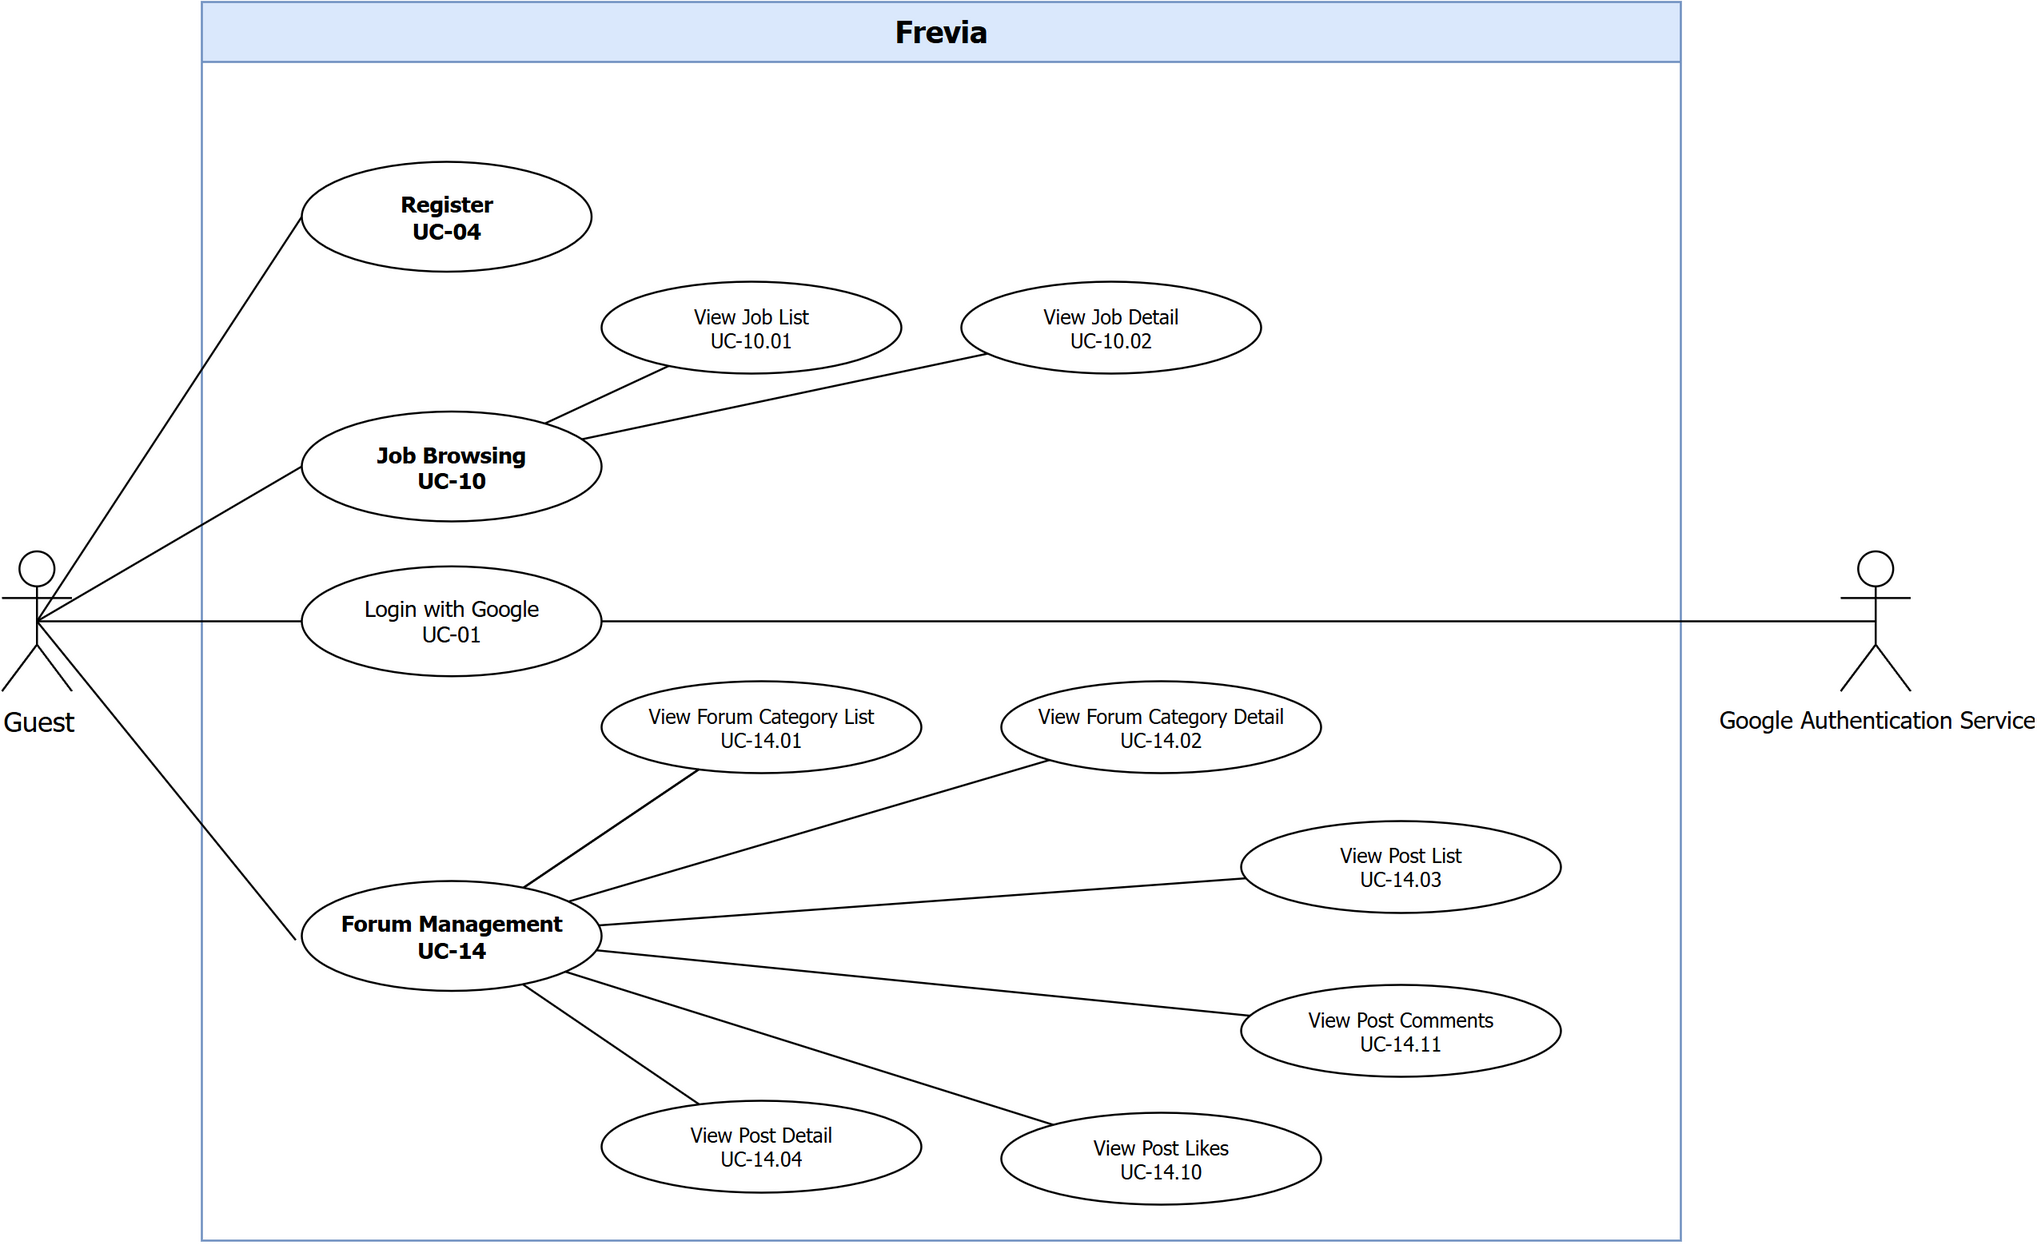
\includegraphics[width=0.95\textwidth]{image/UC_diagram/GUEST_SP1.png}
    \caption{Guest Usecase}
    \label{fig:Guest Usecase}
\end{figure}

% Client

\begin{figure}[H]
    \centering
    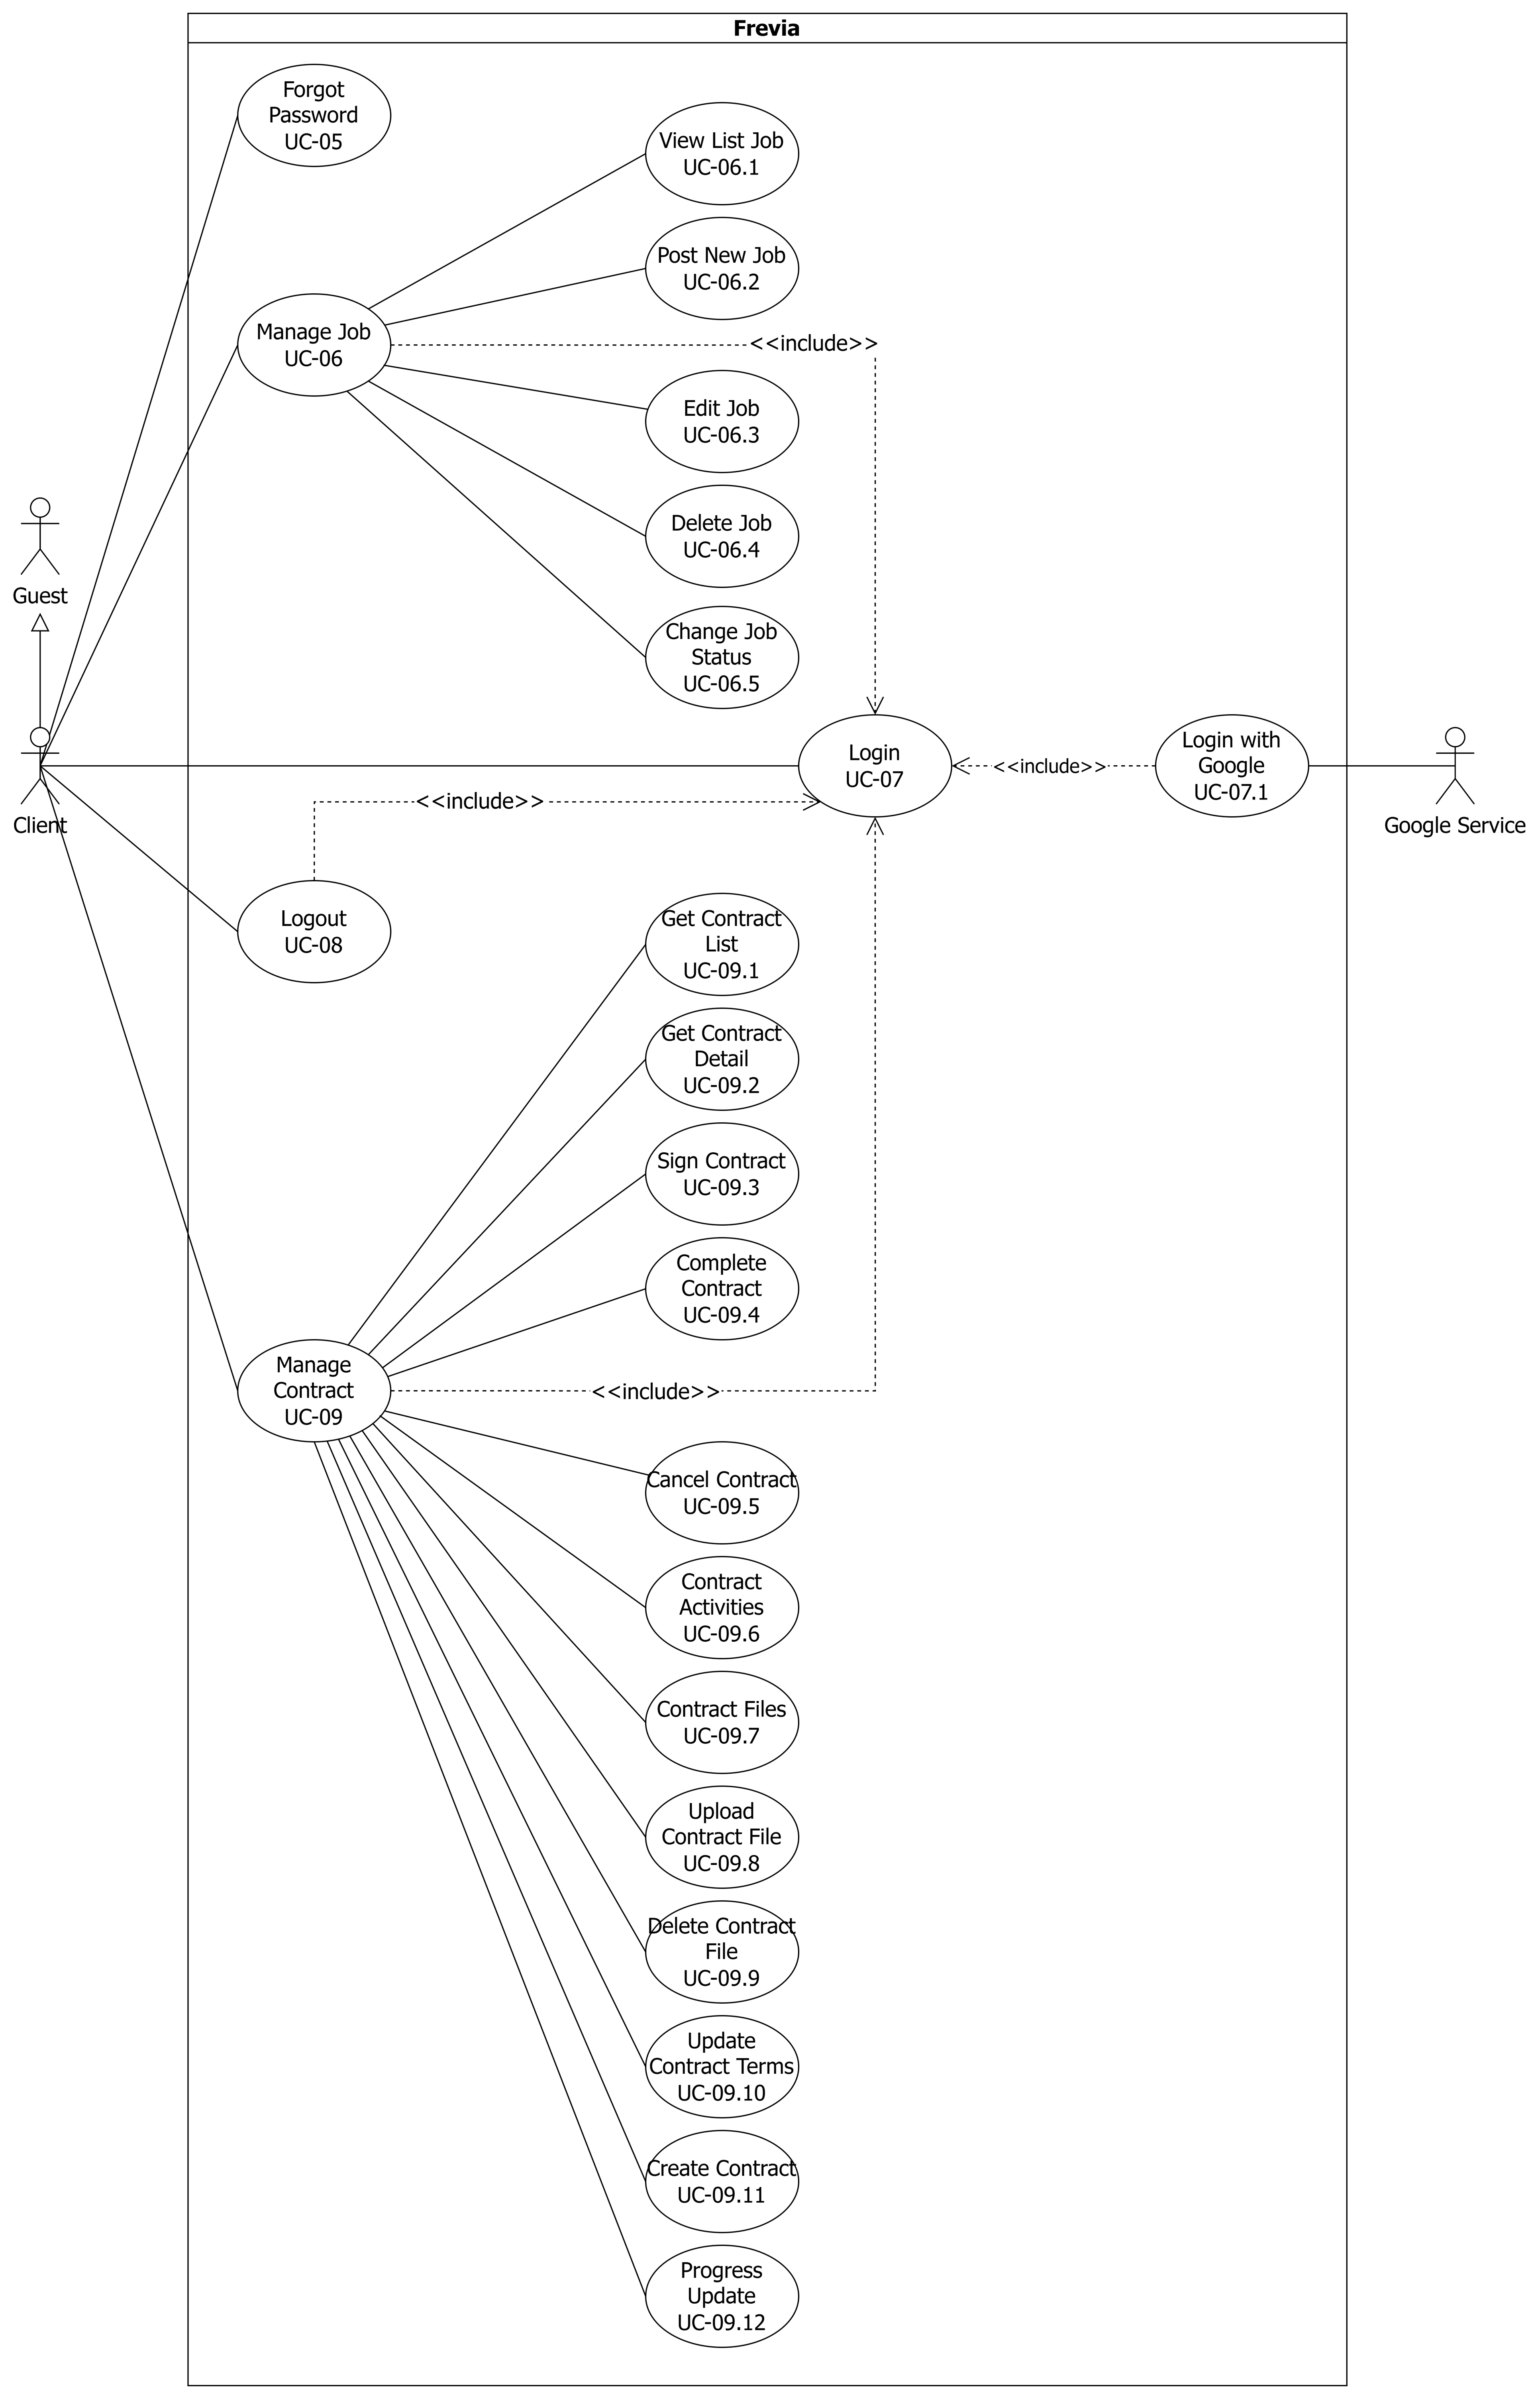
\includegraphics[
            width=\textwidth,
        height=0.85\textheight,
        keepaspectratio
    ]{image/UC_diagram/CLIENT1_SP1.png}
    \caption{Client Usecase}
    \label{fig:Client Usecase 1}
\end{figure}

\begin{figure}[H]
    \centering
    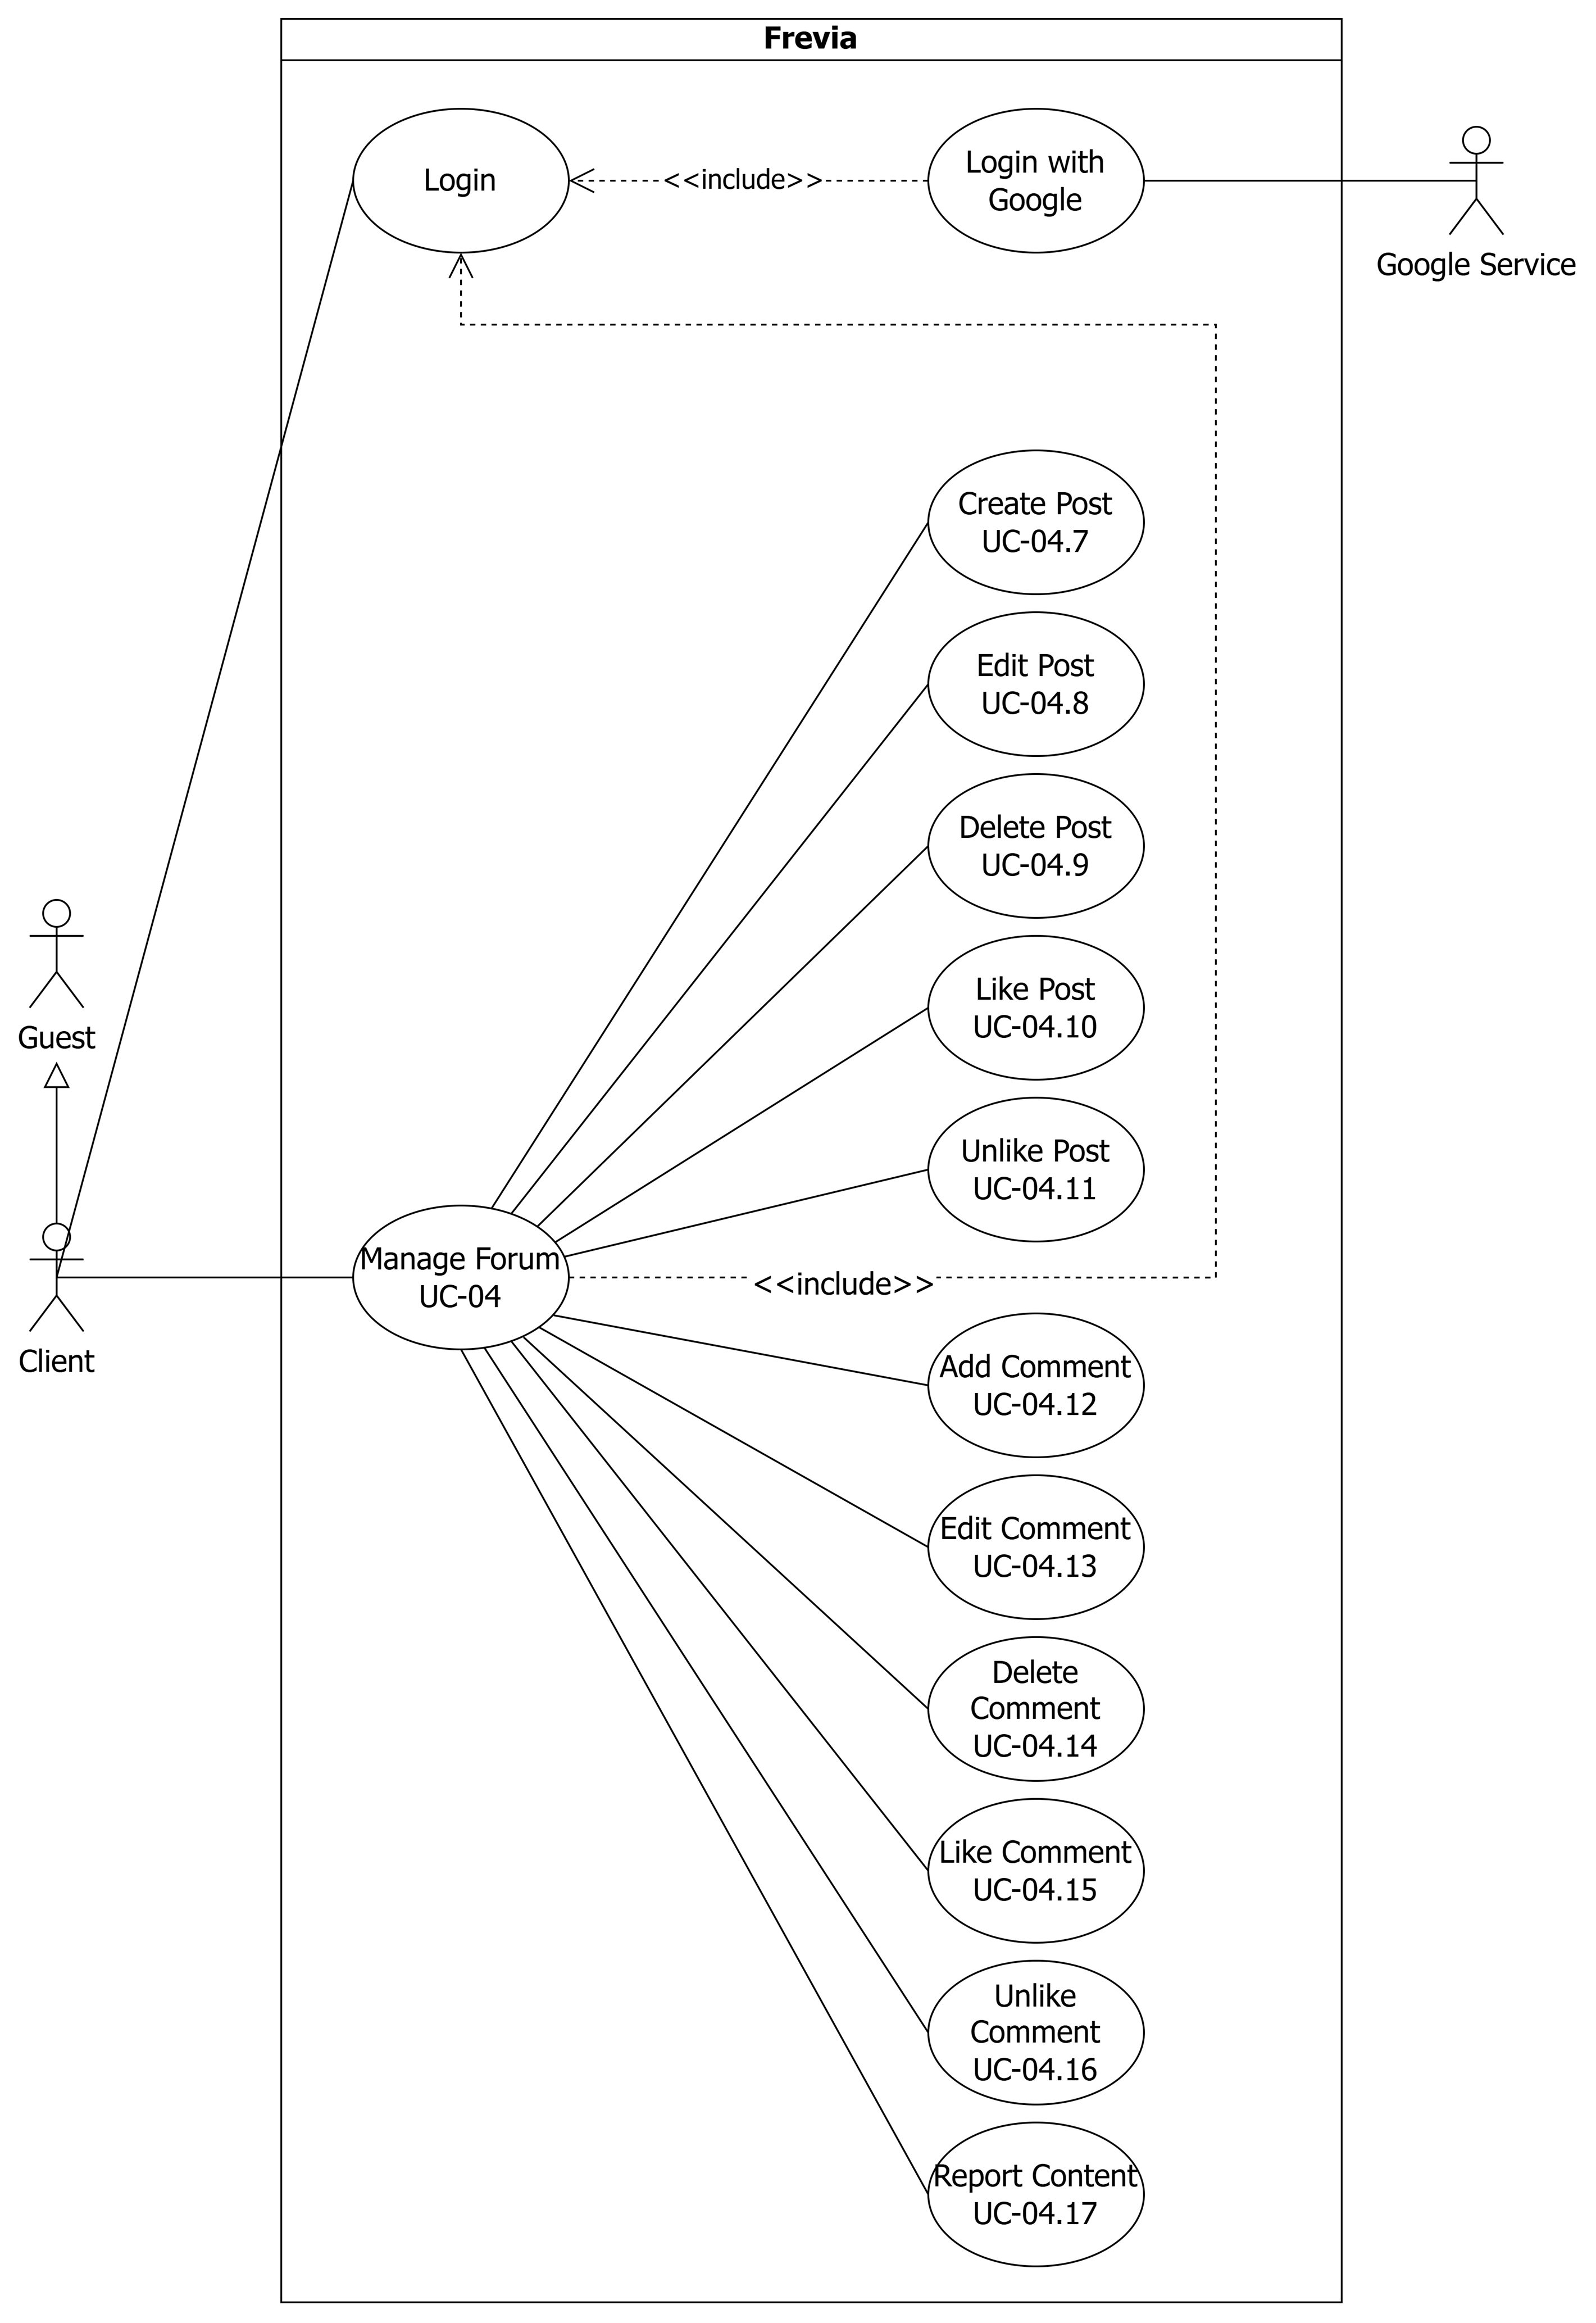
\includegraphics[
            width=\textwidth,
        height=0.85\textheight,
        keepaspectratio
    ]{image/UC_diagram/CLIENT2_SP1.png}
    \caption{Client Usecase}
    \label{fig:Client Usecase 2}
\end{figure}


% Freelancer
\begin{figure}[H]
    \centering
    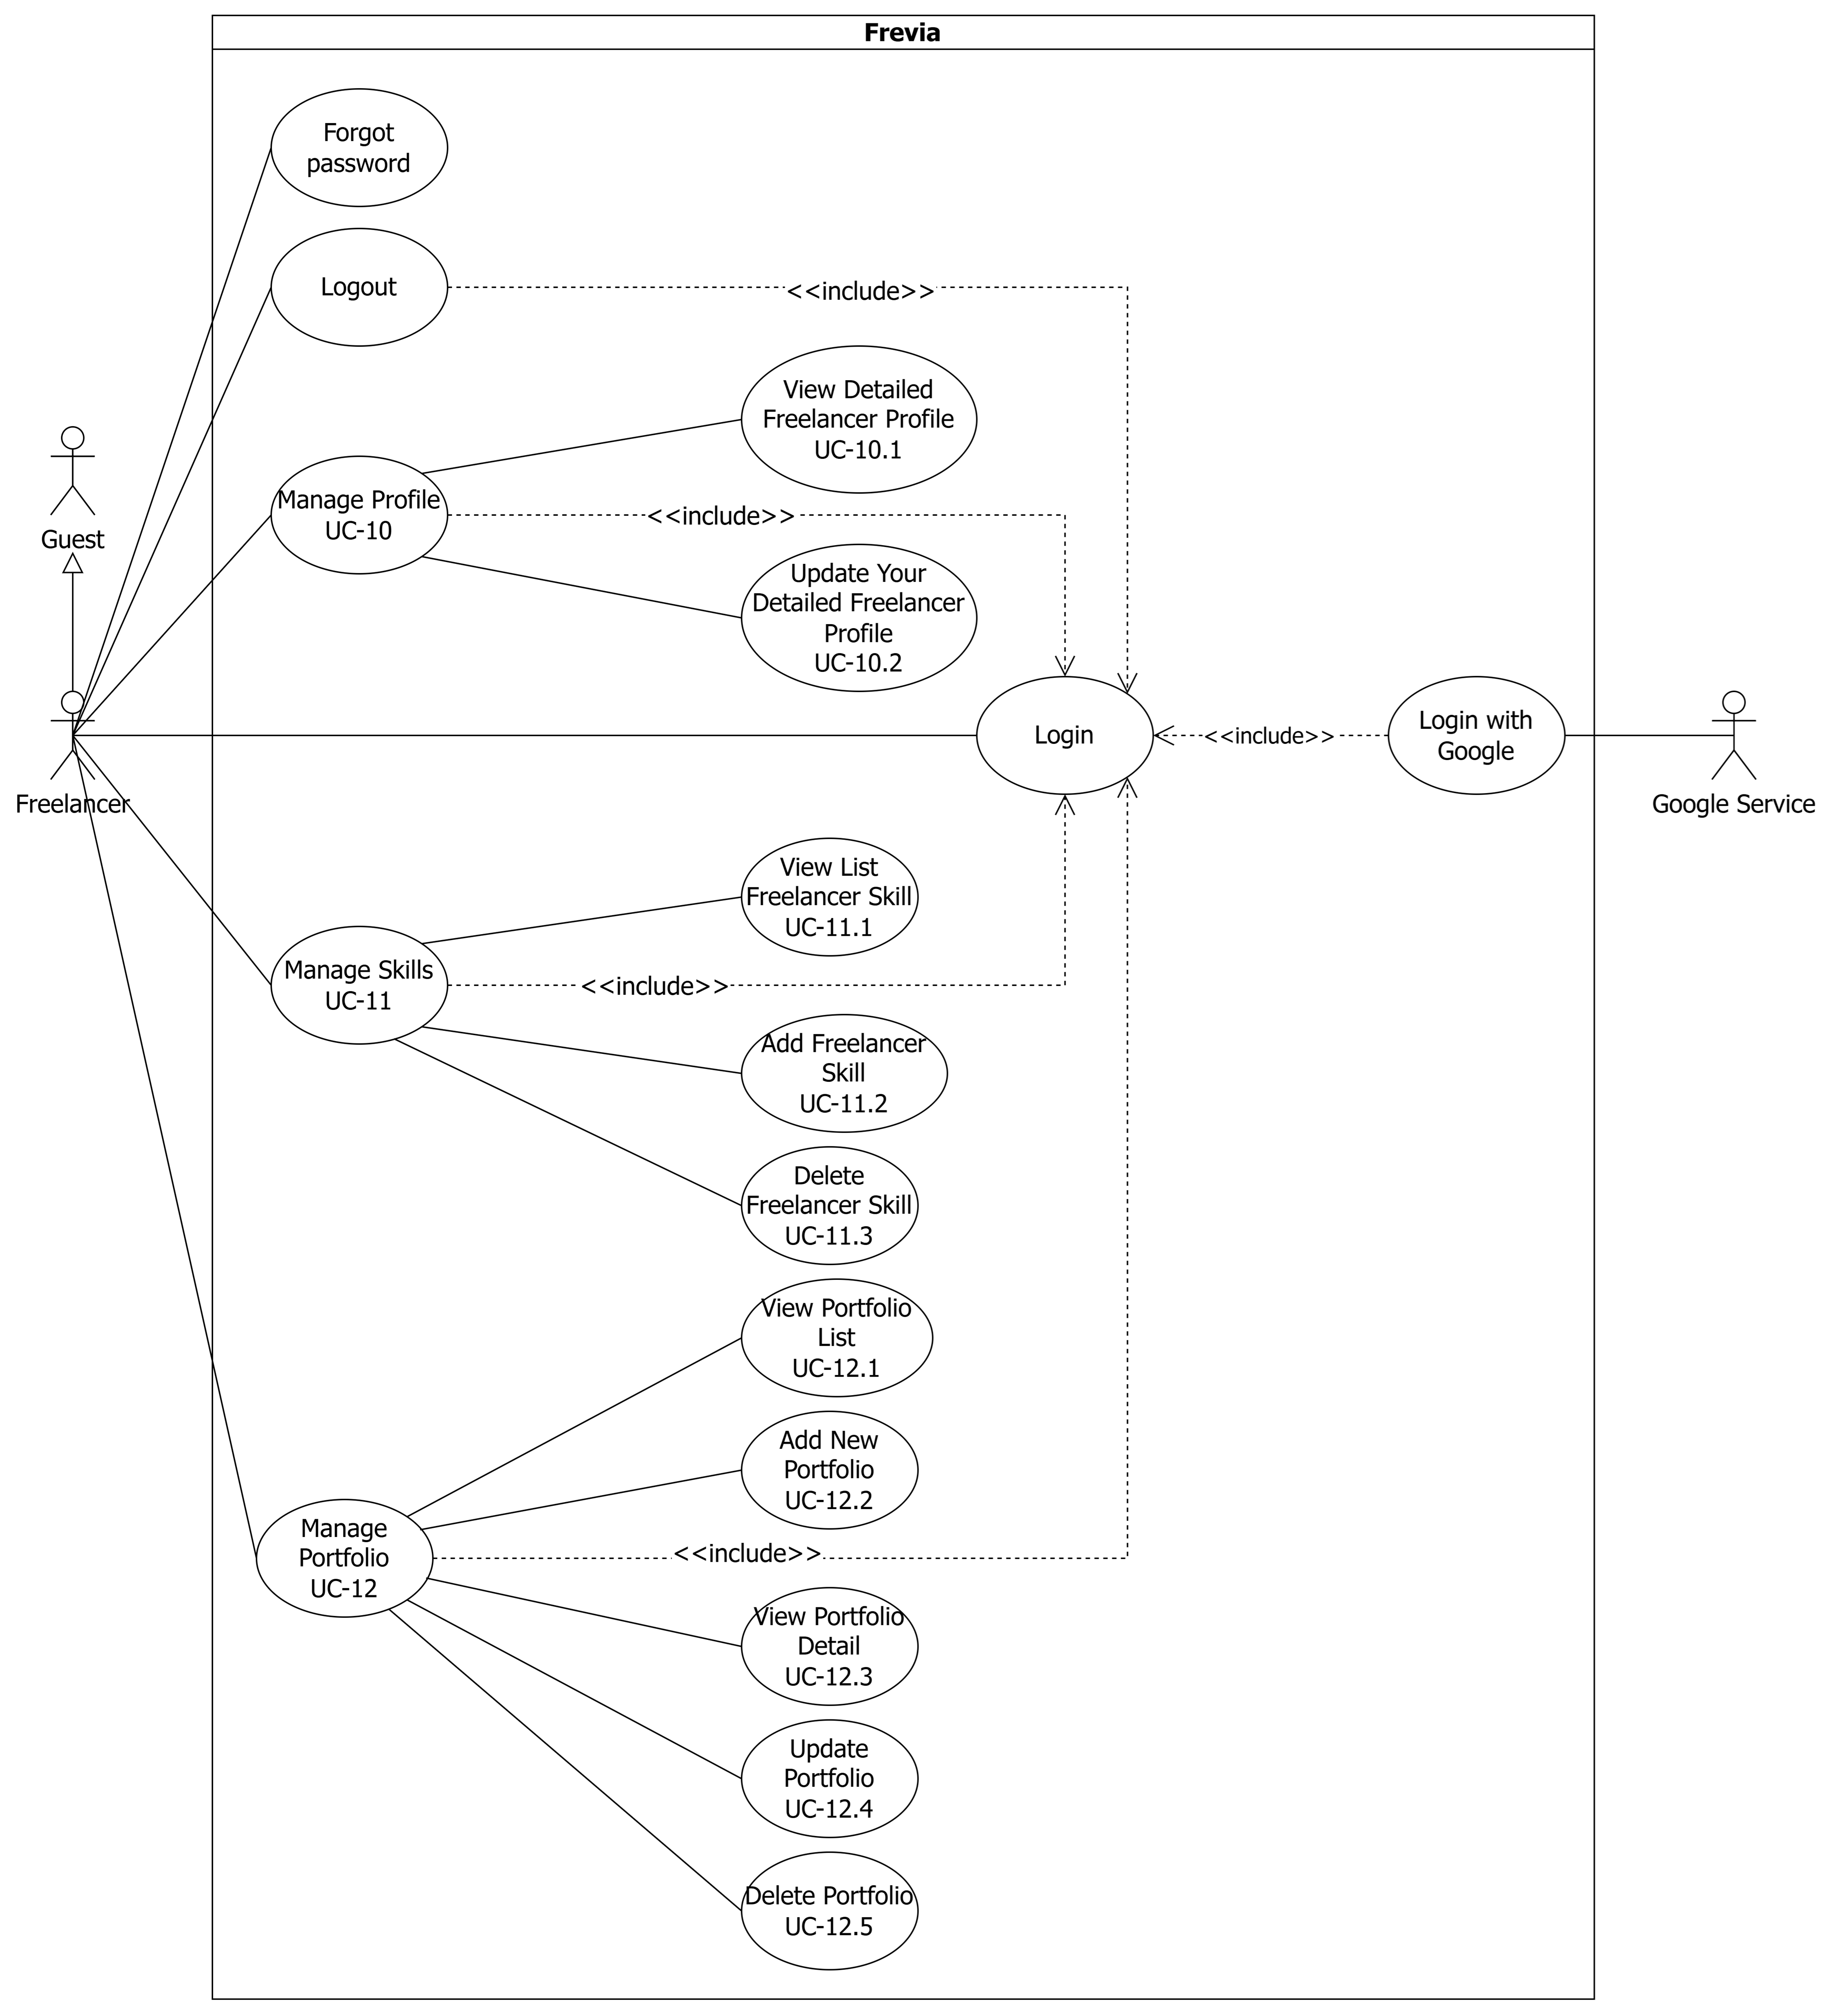
\includegraphics[
            width=\textwidth,
        height=0.85\textheight,
        keepaspectratio
    ]{image/UC_diagram/FREE1_SP1.png}
    \caption{Freelancer Usecase}
    \label{fig:Freelancer Usecase 1}
\end{figure}

\begin{figure}[H]
    \centering
    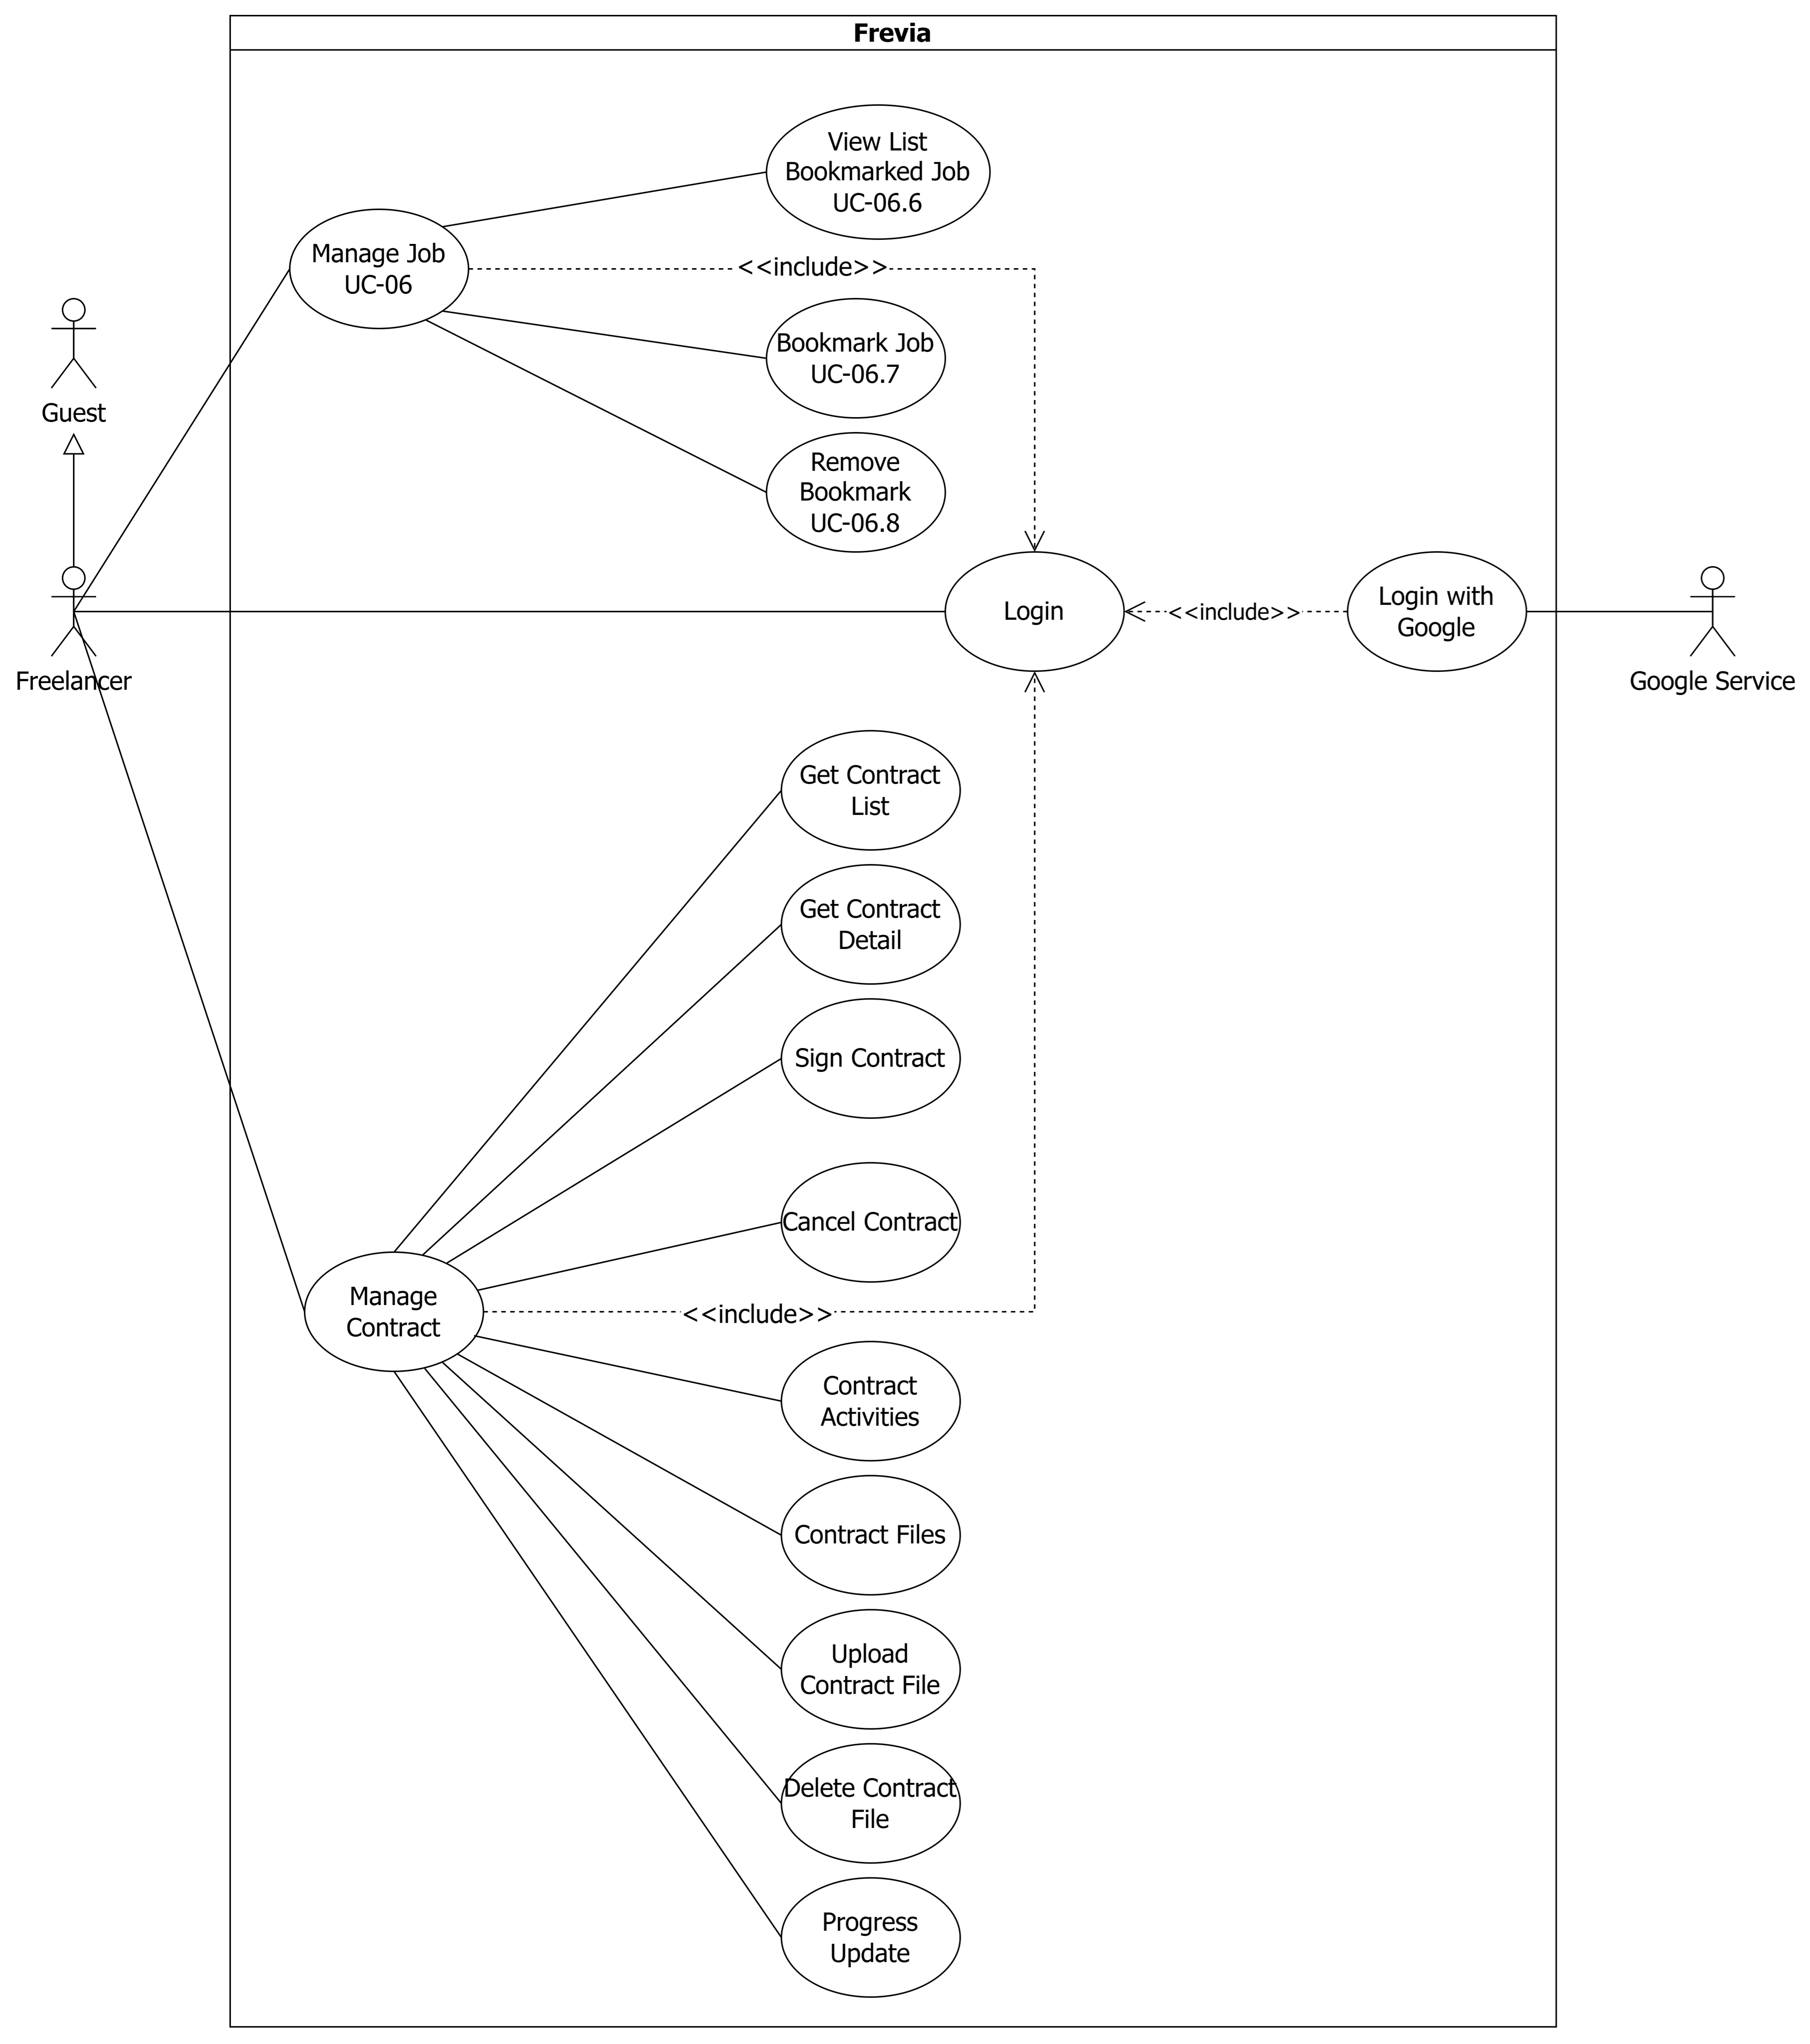
\includegraphics[
            width=\textwidth,
        height=0.85\textheight,
        keepaspectratio
    ]{image/UC_diagram/FREE2_SP1.png}
    \caption{Freelancer Usecase}
    \label{fig:Freelancer Usecase 2}
\end{figure}

\begin{figure}[H]
    \centering
    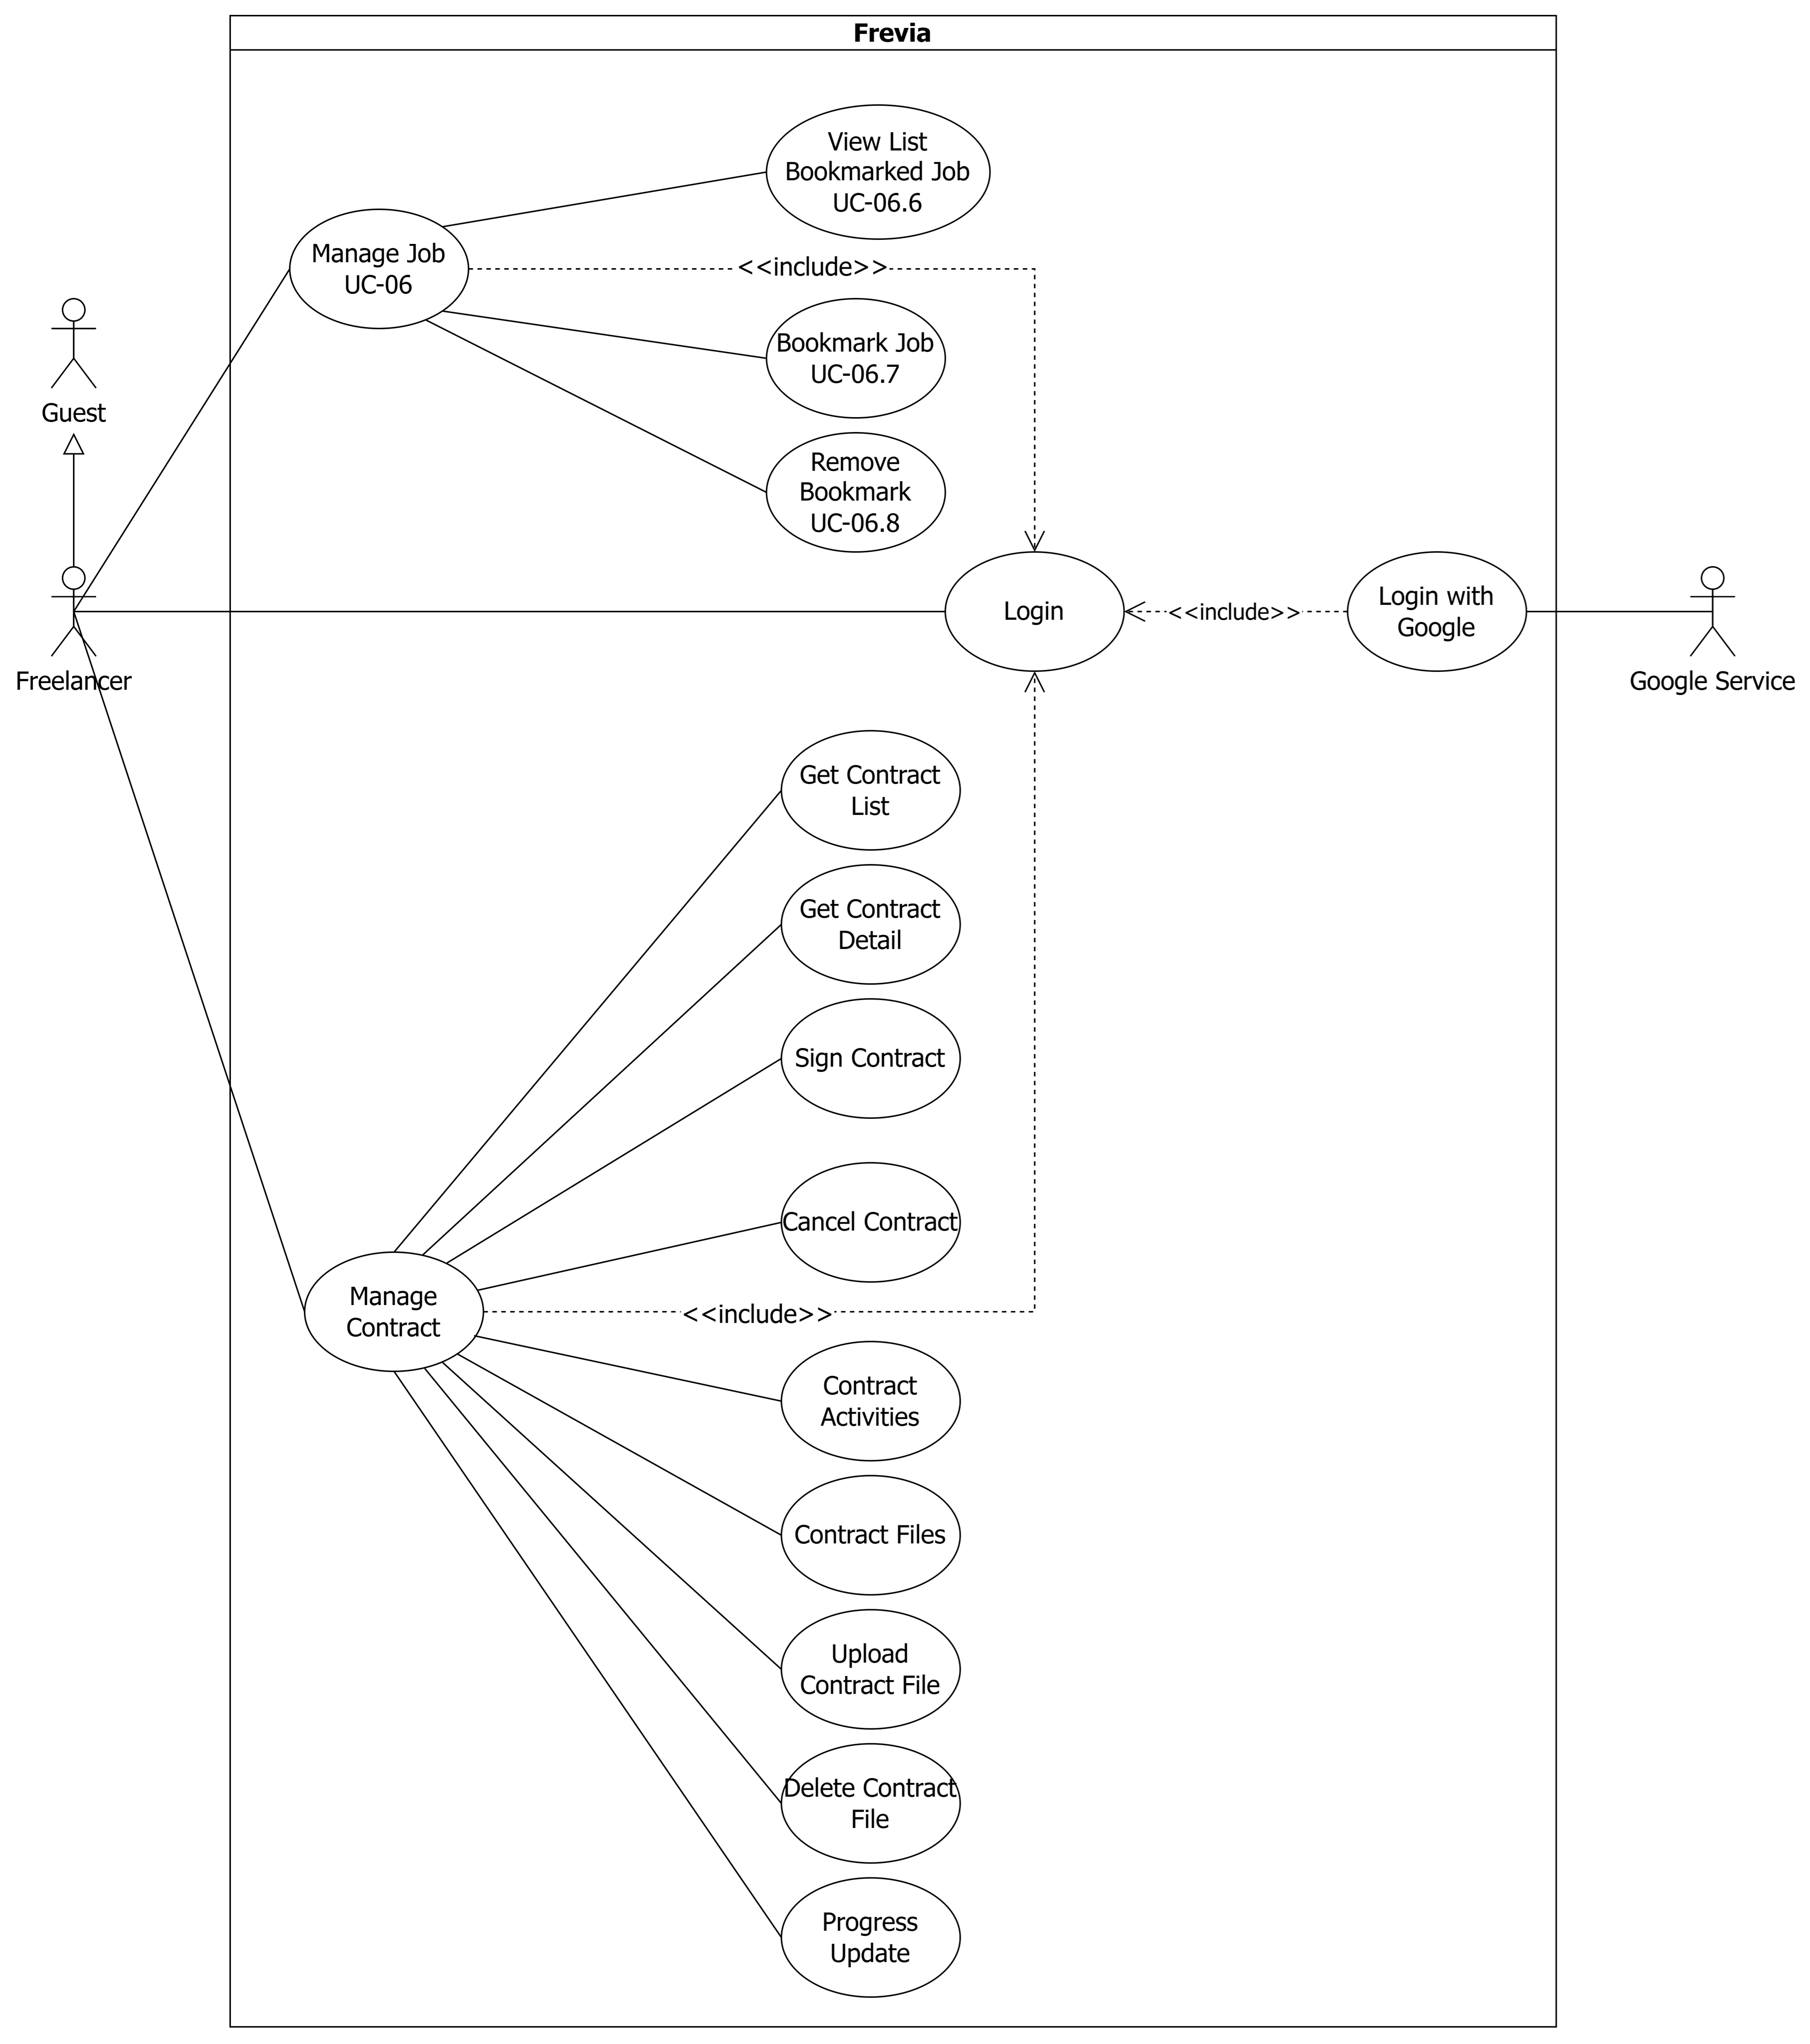
\includegraphics[
            width=\textwidth,
        height=0.85\textheight,
        keepaspectratio
    ]{image/UC_diagram/FREE2_SP1.png}
    \caption{Freelancer Usecase}
    \label{fig:Freelancer Usecase 3}
\end{figure}

% Admin

\begin{figure}[H]
    \centering
    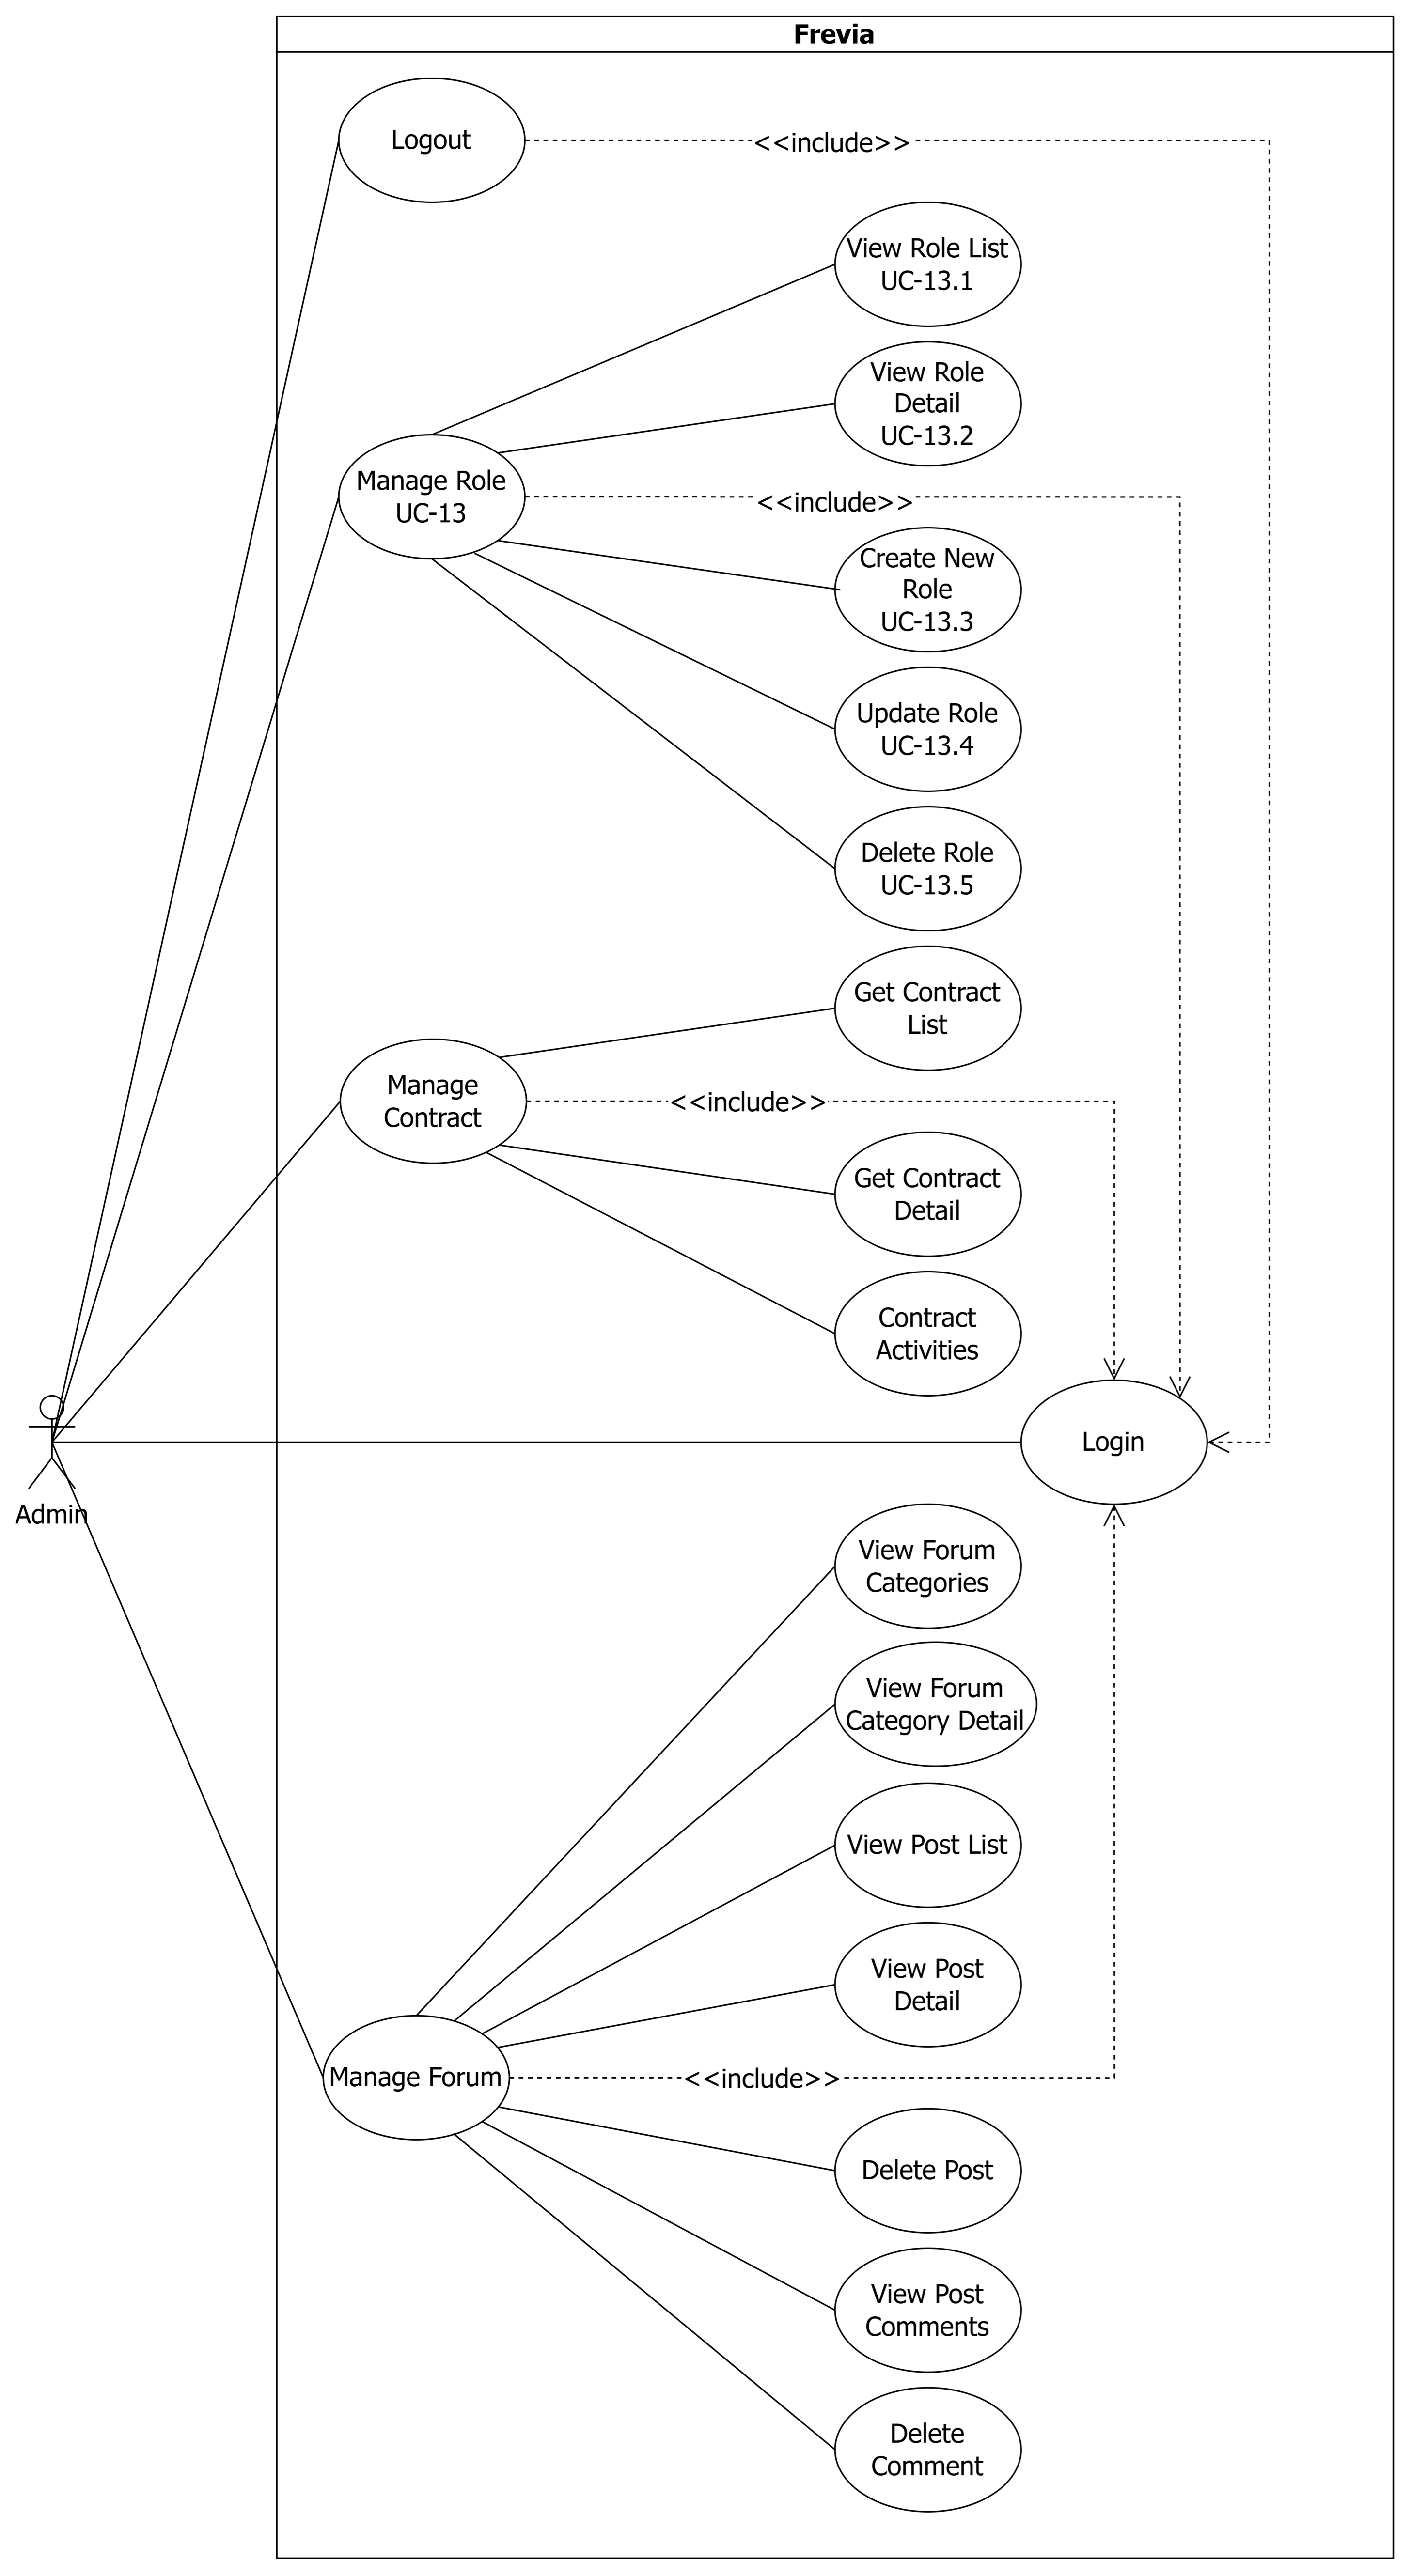
\includegraphics[
            width=\textwidth,
        height=0.85\textheight,
        keepaspectratio
    ]{image/UC_diagram/ADMIN_SP1.png}
    \caption{Admin Usecase}
    \label{fig:Admin Usecase}
\end{figure}
% BEGIN NHUY SPRINT DIAGRAMS
\paragraph{Canonical Sprint Use Cases -- Nguyen Lu Nhat Huy}
These diagrams show the 51 use cases assigned to this author using the final sprint identifiers. Existing diagrams for other authors are retained.
\begin{figure}[H]\centering
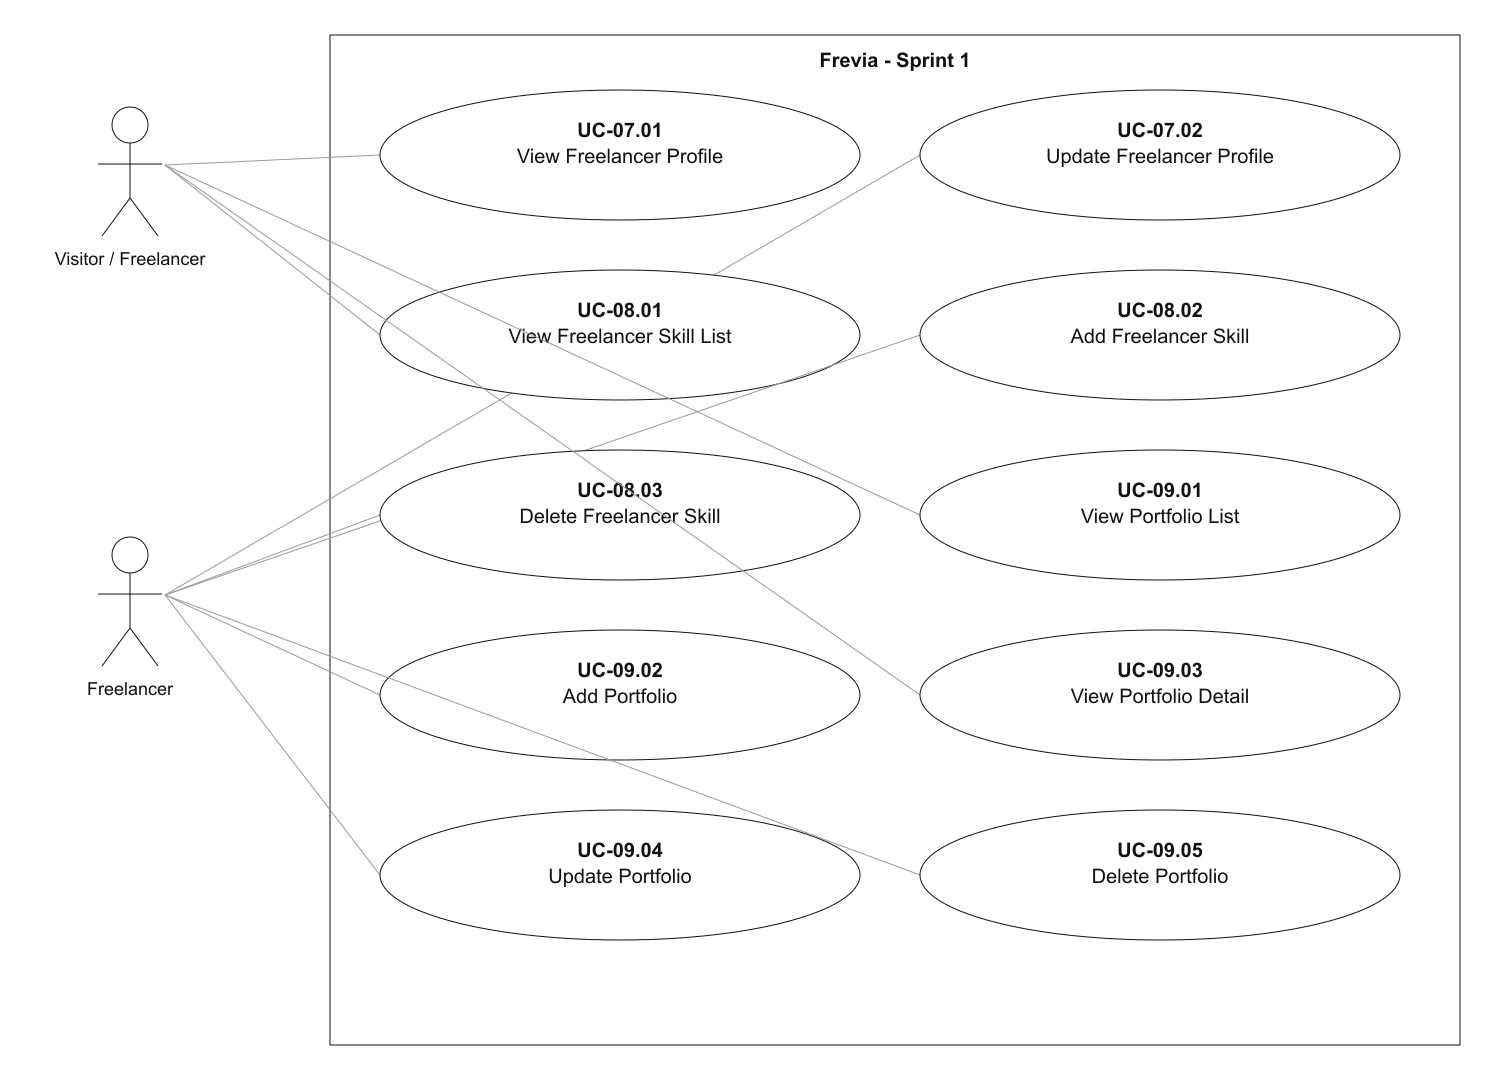
\includegraphics[width=0.98\textwidth,height=0.85\textheight,keepaspectratio]{image/UC_diagram/nhuy-sprint1.png}
\caption{Sprint 1 use cases -- Nguyen Lu Nhat Huy}\label{fig:nhuy-usecases-1}
\end{figure}
\begin{figure}[H]\centering
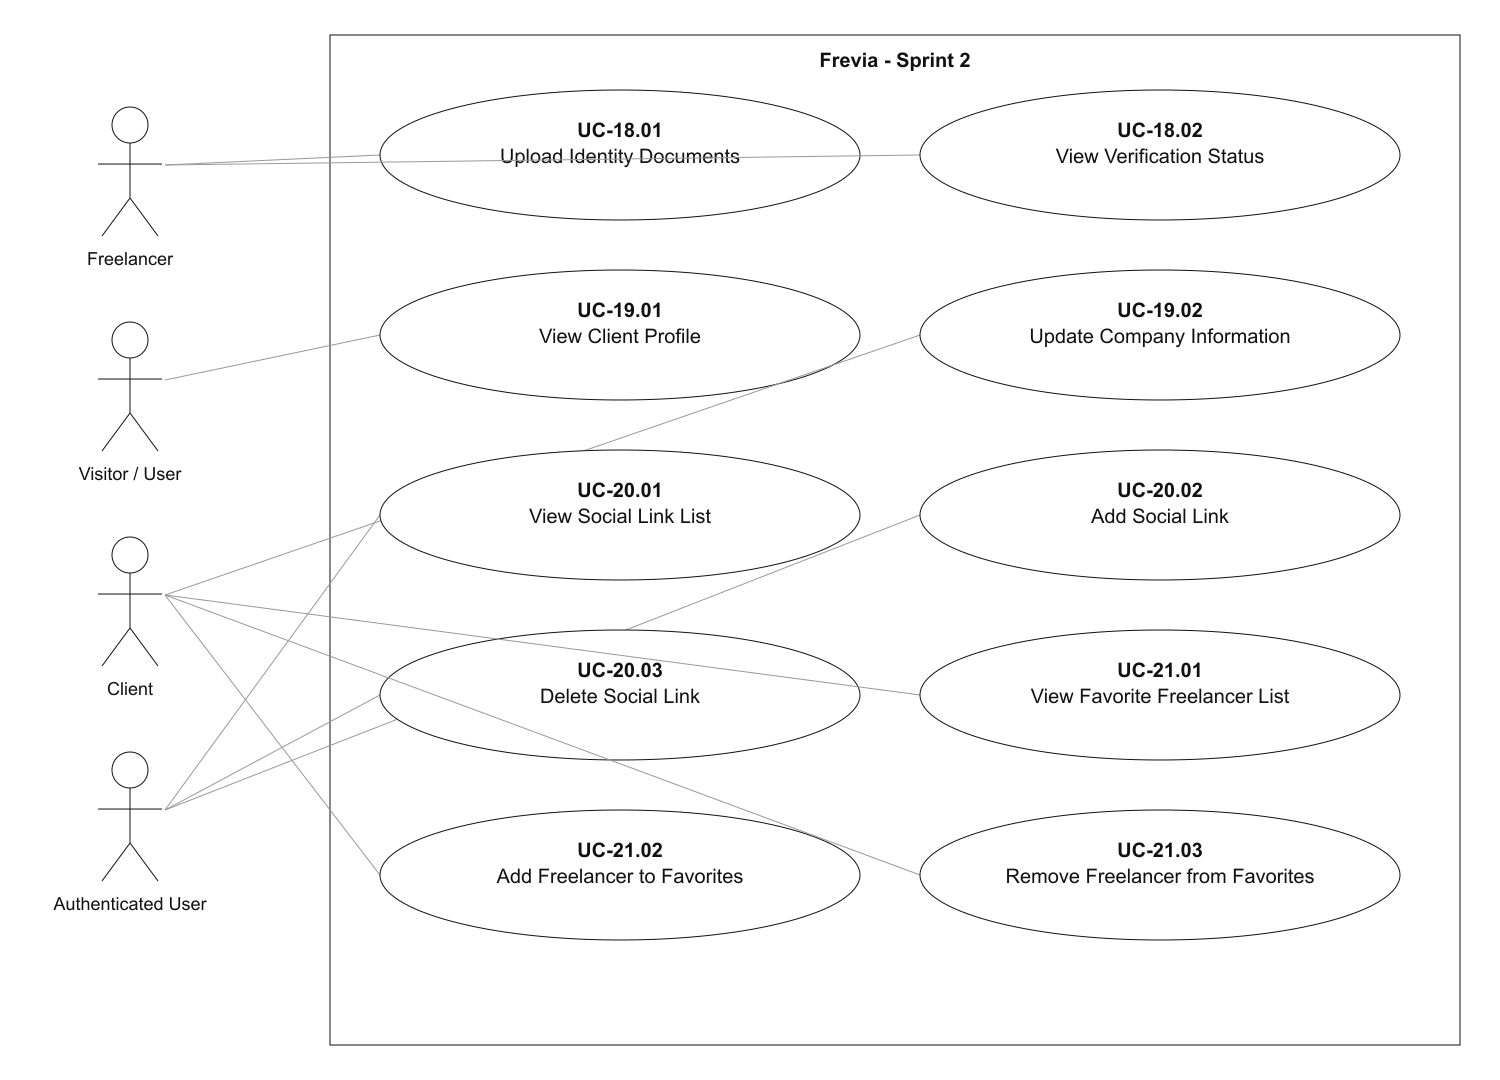
\includegraphics[width=0.98\textwidth,height=0.85\textheight,keepaspectratio]{image/UC_diagram/nhuy-sprint2.png}
\caption{Sprint 2 use cases -- Nguyen Lu Nhat Huy}\label{fig:nhuy-usecases-2}
\end{figure}
\begin{figure}[H]\centering
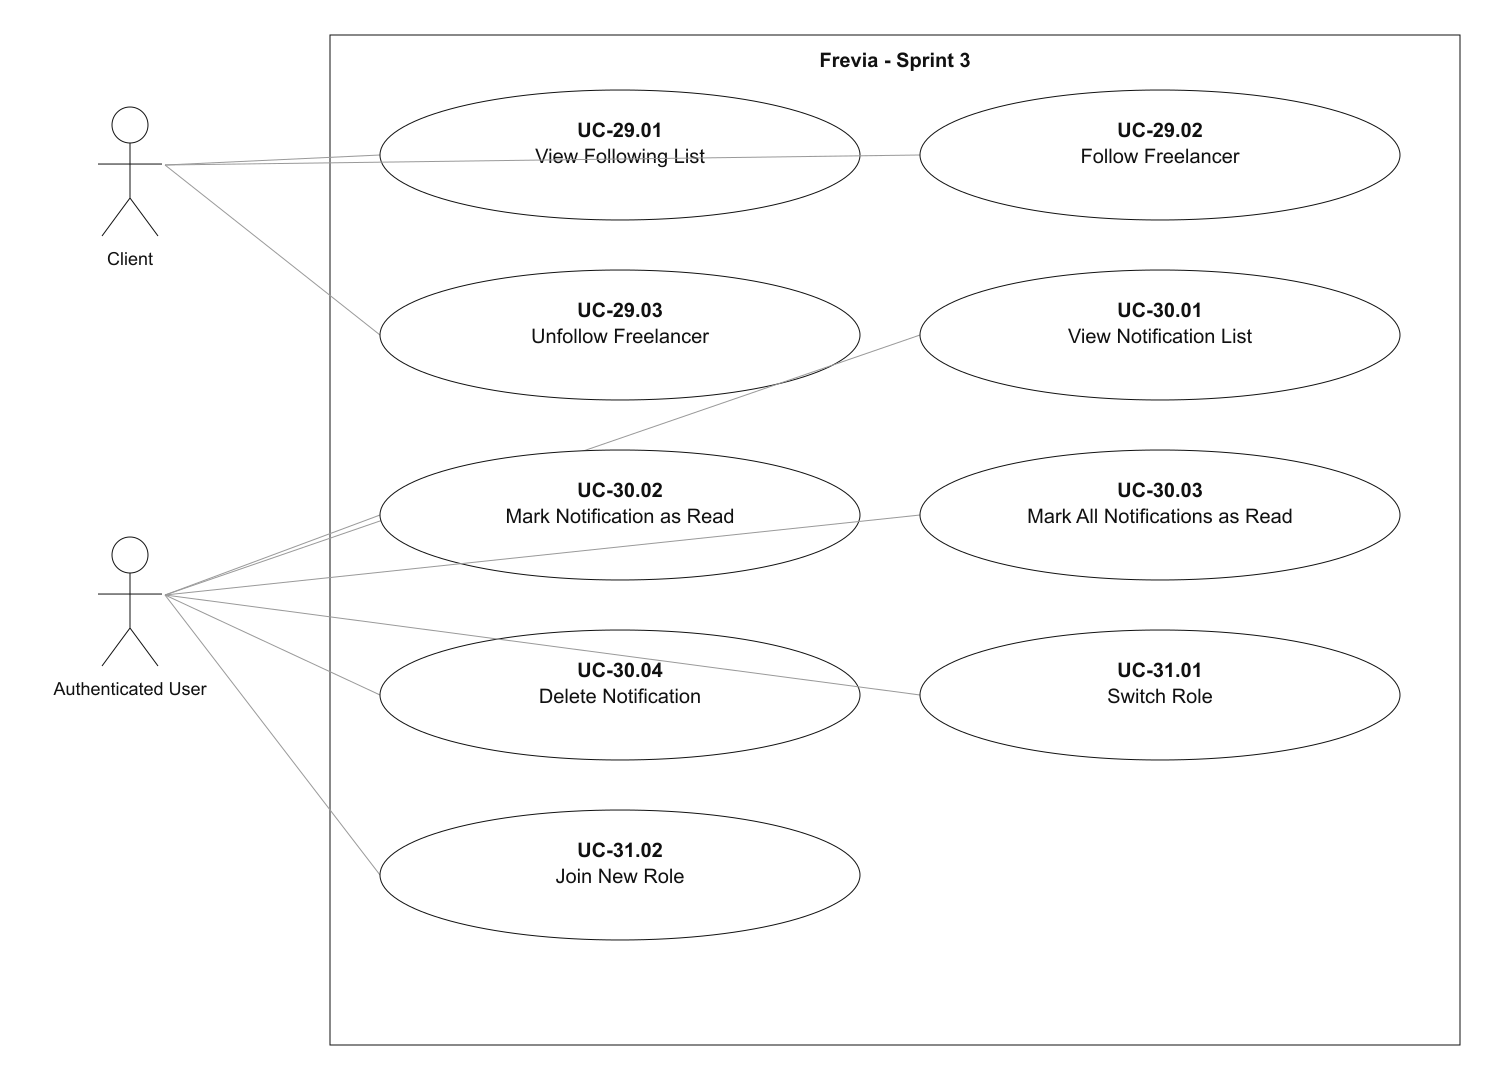
\includegraphics[width=0.98\textwidth,height=0.85\textheight,keepaspectratio]{image/UC_diagram/nhuy-sprint3.png}
\caption{Sprint 3 use cases -- Nguyen Lu Nhat Huy}\label{fig:nhuy-usecases-3}
\end{figure}
\begin{figure}[H]\centering
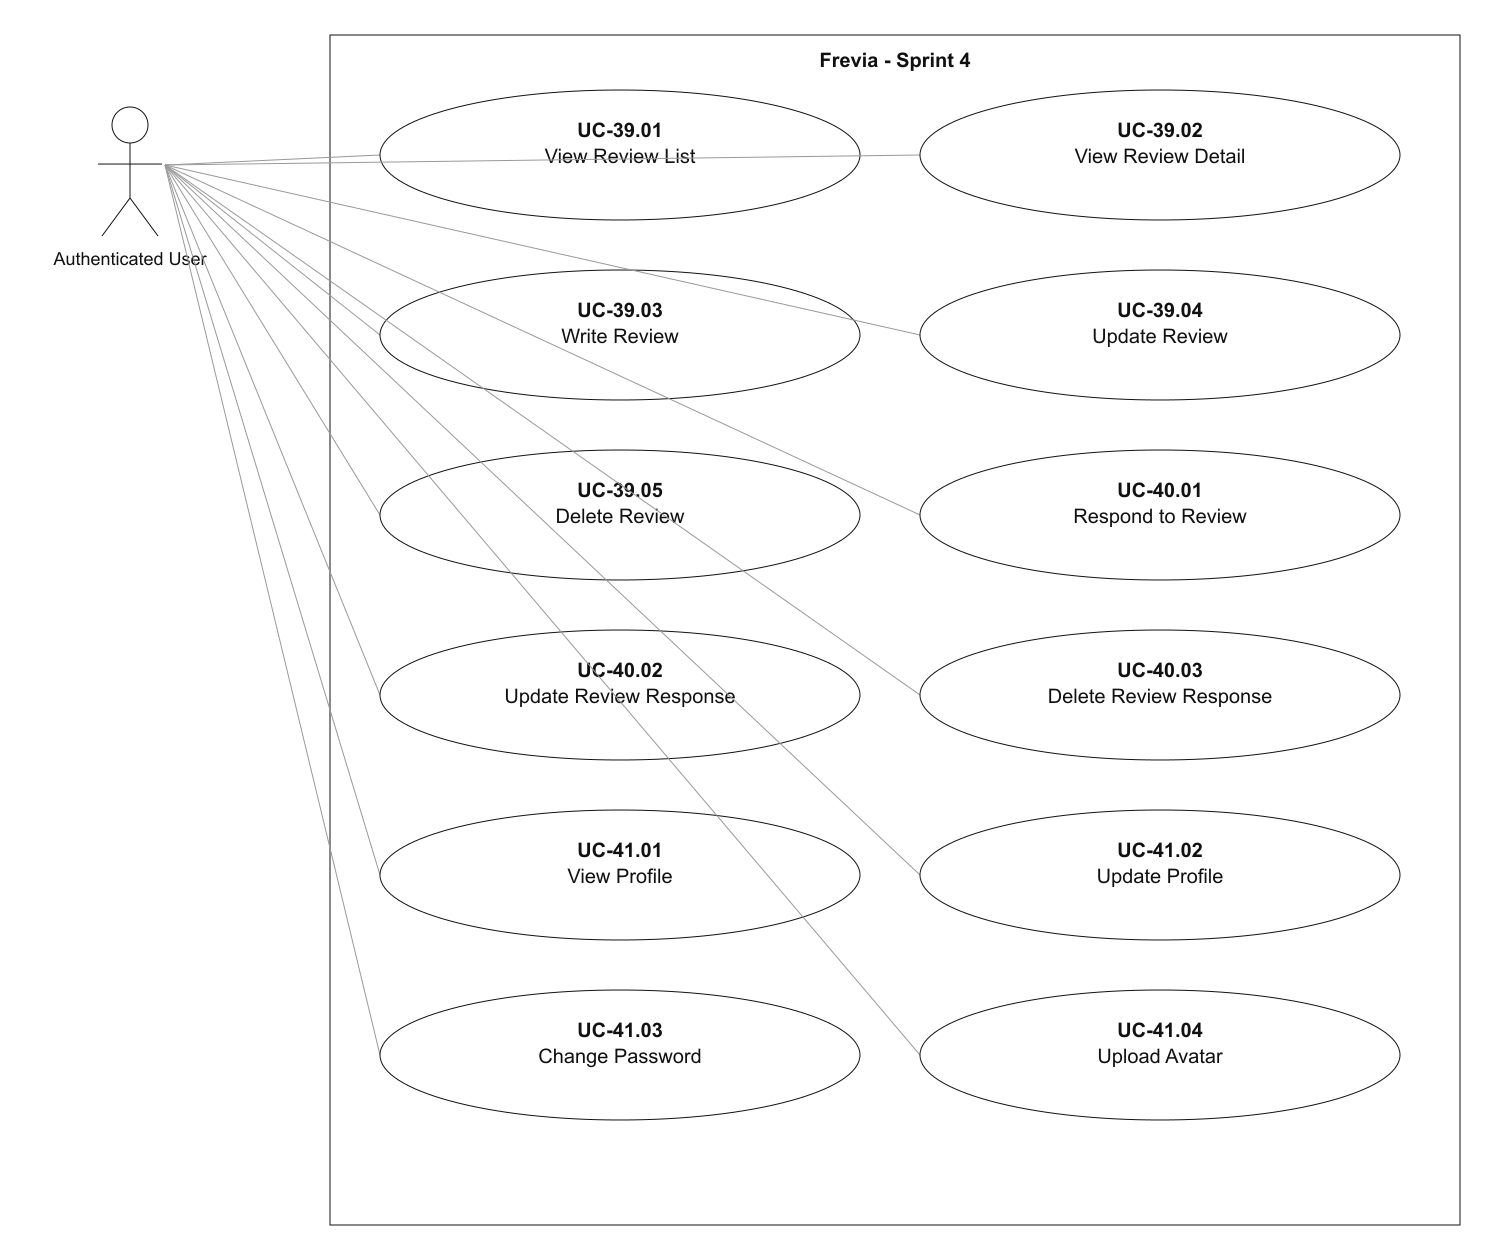
\includegraphics[width=0.98\textwidth,height=0.85\textheight,keepaspectratio]{image/UC_diagram/nhuy-sprint4.png}
\caption{Sprint 4 use cases -- Nguyen Lu Nhat Huy}\label{fig:nhuy-usecases-4}
\end{figure}
\begin{figure}[H]\centering
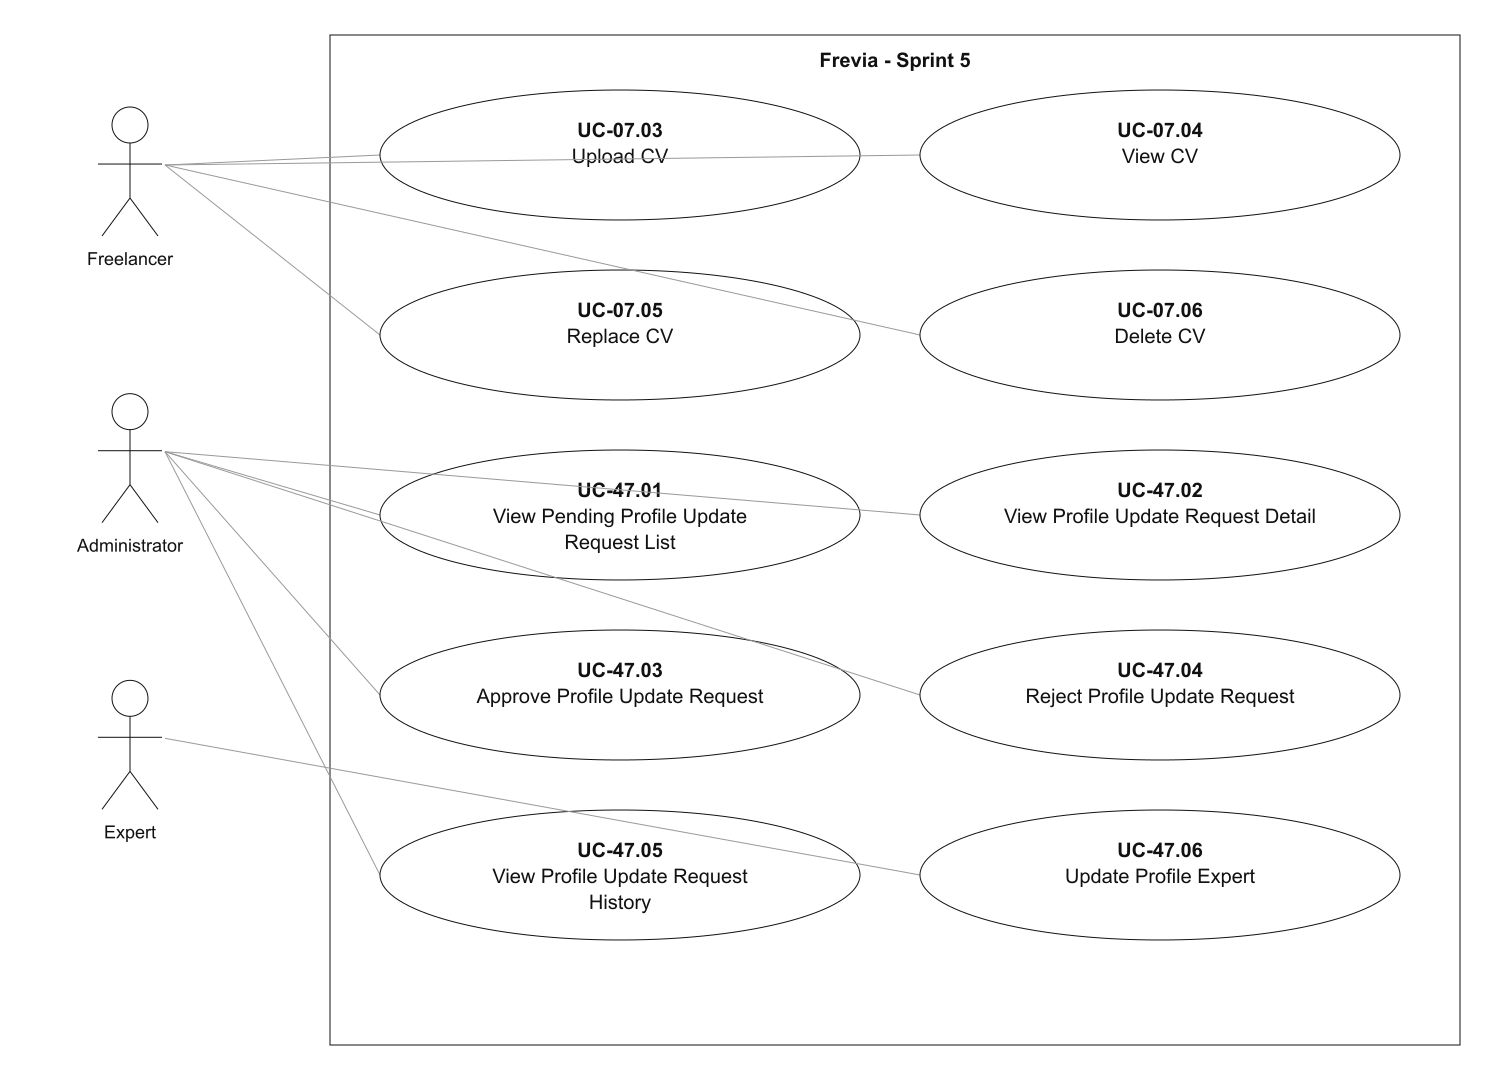
\includegraphics[width=0.98\textwidth,height=0.85\textheight,keepaspectratio]{image/UC_diagram/nhuy-sprint5.png}
\caption{Sprint 5 use cases -- Nguyen Lu Nhat Huy}\label{fig:nhuy-usecases-5}
\end{figure}
% END NHUY SPRINT DIAGRAMS


\subsubsection{Descriptions}
\begin{longtable}{|>{\raggedright\arraybackslash}p{2.2cm}|>{\raggedright\arraybackslash}p{3cm}|>{\raggedright\arraybackslash}p{3cm}|>{\raggedright\arraybackslash}p{7.5cm}|}
\hline
\rowcolor{headerbg}
\multicolumn{1}{|>{\raggedright\arraybackslash}p{2.2cm}|}{\textbf{ID}} &
\multicolumn{1}{>{\raggedright\arraybackslash}p{3cm}|}{\textbf{Use Case}} &
\multicolumn{1}{>{\raggedright\arraybackslash}p{3cm}|}{\textbf{Actors}} &
\multicolumn{1}{>{\raggedright\arraybackslash}p{7.5cm}|}{\textbf{Description}} \\
\hline
\endfirsthead

\hline
\rowcolor{headerbg}
\multicolumn{1}{|>{\raggedright\arraybackslash}p{2.2cm}|}{\textbf{ID}} &
\multicolumn{1}{>{\raggedright\arraybackslash}p{3cm}|}{\textbf{Use Case}} &
\multicolumn{1}{>{\raggedright\arraybackslash}p{3cm}|}{\textbf{Actors}} &
\multicolumn{1}{>{\raggedright\arraybackslash}p{7.5cm}|}{\textbf{Description}} \\
\hline
\endhead

\hline
\multicolumn{4}{r}{\textit{Continued on next page}} \\
\endfoot

\hline
\endlastfoot


UC-01 & Login with Google & Guest & Allows users to login/register using Google OAuth. \\
\hline
UC-02 & Login & Guest & Allows users to log in using email/password and JWT authentication. \\
\hline
UC-03 & Logout & Client, Expert, Freelancer, Admin & Allows users to logout and terminate authentication session. \\
\hline
UC-04 & Register & Guest & Allows users to create new accounts using email and password. \\
\hline
UC-05 & Forgot Password & Guest & Allows users to request password reset via email verification link. \\
\hline
UC-06.01 & View Role List & Admin & Retrieve list of all roles along with their assigned permissions. \\
\hline
UC-06.02 & View Role Detail & Admin & View detailed information of a specific role including its permissions. \\
\hline
UC-06.03 & Create Role & Admin & Create a new role with name, description, and a list of permission IDs. \\
\hline
UC-06.04 & Update Role & Admin & Update a role's name, description, and replace all assigned permissions. \\
\hline
UC-06.05 & Delete Role & Admin & Delete a role from the system. \\
\hline
UC-06.06 & Update Role Permissions & Admin & Assign route access rights to roles. \\
\hline
UC-15.01 & View Permission List & Admin & Retrieve all permissions (id, name, path, method, module) for admin to assign to roles. \\
\hline
UC-15.02 & View Permission Detail & Admin & View detailed information of a specific permission. \\
\hline
UC-16.01 & View Session List & Client, Expert, Freelancer, Admin & View a list of active login sessions. \\
\hline
UC-16.02 & View Session Detail & Client, Expert, Freelancer, Admin & View login session information (device, IP address, login time, approximate location, etc.). \\
\hline
UC-16.03 & Revoke Session & Client, Expert, Freelancer, Admin & Log out of a specific device remotely. \\
\hline
UC-17.01 & Create Forum Category & Admin & Allows admins to create a new forum category. \\
\hline
UC-17.02 & Update Forum Category & Admin & Allows admins to update an existing forum category. \\
\hline
UC-17.03 & Delete Forum Category & Admin & Allows admins to soft-delete a forum category. \\
\hline
UC-14.01 & View Forum Category List & Admin & Allows admins to view the list of forum categories. \\
\hline
UC-14.02 & View Forum Category Detail & Admin & Allows admins to view the details of a specific forum category. \\
\hline
UC-17.06 & Restore Forum Category & Admin & Restore a deleted Category forum by setting deletedAt back to null. \\
\hline
UC-03 & Job Browsing & Guest, Client, Freelancer & Enables guests to browse and search for available job listings. \\
\hline
UC-03.1 & View List Job & Guest, Client, Freelancer & Retrieve paginated job list with filters (category, budget, skills, status, keywords) and sorting options. \\
\hline
UC-03.2 & View Job Detail & Guest, Client, Freelancer & Get full job details: title, description, budget, skills, client info, proposals count, attachments, timeline. \\
\hline
UC-04 & Manage Forum & Guest, Client, Freelancer, Admin & Manages forum operations including viewing, creating, editing, and moderating posts and comments. \\
\hline
UC-04.1 & View Forum Categories & Guest, Client, Freelancer, Admin & Displays all available forum categories for browsing. \\
\hline
UC-04.2 & View Forum Category Detail & Guest, Client, Freelancer, Admin & Shows detailed information of a specific forum category and its sub-forums. \\
\hline
UC-04.3 & View Post List & Guest, Client, Freelancer, Admin & Retrieves paginated list of posts within a forum category with filters and sorting. \\
\hline
UC-04.4 & View Post Detail & Guest, Client, Freelancer, Admin & Displays full post content, author info, creation date, and associated tags. \\
\hline
UC-04.5 & View Comments & Guest, Client, Freelancer, Admin & Retrieves all comments related to a specific forum post. \\
\hline
UC-04.6 & View Comment Detail & Guest, Client, Freelancer, Admin & Shows detailed information of a specific comment, including content, author, and timestamps. \\
\hline
UC-04.7 & Create Post & Client, Freelancer & Allows freelancers to create new discussion posts or questions in the forum. \\
\hline
UC-04.8 & Edit Post & Client, Freelancer & Allows freelancers to edit their own forum posts. \\
\hline
UC-04.9 & Delete Post & Client, Freelancer, Admin & Allows post owners or admins to delete a forum post. \\
\hline
UC-04.10 & Like Post & Client, Freelancer & Allows freelancers to like a forum post. \\
\hline
UC-04.11 & Unlike Post & Client, Freelancer & Allows freelancers to remove their like from a forum post. \\
\hline
UC-04.12 & Add Comment & Client, Freelancer & Allows freelancers to add comments to a forum post. \\
\hline
UC-04.13 & Edit Comment & Client, Freelancer & Allows freelancers to edit their own comments. \\
\hline
UC-04.14 & Delete Comment & Client, Freelancer & Allows comment owners or admins to delete a comment. \\
\hline
UC-04.15 & Like Comment & Client, Freelancer & Allows freelancers to like a comment. \\
\hline
UC-04.16 & Unlike Comment & Client, Freelancer & Allows freelancers to remove their like from a comment. \\
\hline
UC-04.17 & Report Content & Client, Freelancer & Allows freelancers to report inappropriate content in forum posts or comments. \\
\hline
UC-06 & Manage Job & Client, Freelancer & Manages job postings including creation, editing, deletion, and status changes. \\
\hline
UC-06.1 & View List Job & Guest, Client, Freelancer & Retrieve paginated job list with filters and sorting options. \\
\hline
UC-06.2 & Post New Job & Client & Allows clients to create and publish new job postings. \\
\hline
UC-06.3 & Edit Job & Client & Allows clients to edit their own job postings. \\
\hline
UC-06.4 & Delete Job & Client & Allows clients to delete their own job postings. \\
\hline
UC-06.5 & Change Job Status & Client & Allows clients to update job status (Open, In Progress, Closed, Cancelled). \\
\hline
UC-06.6 & View List Bookmarked Job & Freelancer & Retrieves list of jobs bookmarked by the freelancer. \\
\hline
UC-06.7 & Bookmark Job & Freelancer & Allows freelancers to save/bookmark a job for later reference. \\
\hline
UC-06.8 & Remove Bookmark & Freelancer & Allows freelancers to remove a bookmarked job from their list. \\
\hline
UC-13 & Manage Contract & Client, Freelancer, Admin & Manages contractual agreements, milestones, deliverables, and file exchanges. \\
\hline
UC-13.01 & Create Contract & Client & Allows clients to create and initiate a new contract with a freelancer. \\
\hline
UC-13.02 & Update Contract & Client & Allows clients to update contract terms, budget, milestones, or deadlines before signing. \\
\hline
UC-13.03 & Complete Contract & Client, Freelancer & Marks an active contract as completed after all milestones are approved and settled. \\
\hline
UC-13.04 & View Contract List & Client, Freelancer, Admin & Retrieves paginated list of contracts with status filters and sorting. \\
\hline
UC-13.05 & View Contract Detail & Client, Freelancer, Admin & Displays full contract details including terms, parties, status, and milestones. \\
\hline
UC-13.06 & Sign Contract & Freelancer, Client & Allows users to digitally accept and sign a contract to activate it. \\
\hline
UC-13.07 & Cancel Contract & Client, Freelancer & Allows either party to cancel or terminate a contract prior to completion. \\
\hline
UC-13.08 & View Contract Files & Client, Freelancer, Admin & Manages and accesses all files and documentation associated with a contract. \\
\hline
UC-13.09 & Upload Contract File & Client, Freelancer & Allows users to upload documents and deliverables to the contract workspace. \\
\hline
UC-13.10 & Delete Contract File & Client, Freelancer, Admin & Allows the uploader or admin to delete files from a contract workspace. \\
\hline
UC-10 & Manage Profile & Freelancer & Manages freelancer profile information and settings. \\
\hline
UC-10.1 & View Detailed Freelancer Profile & Freelancer & Displays full freelancer profile including skills, portfolio, experience, and ratings. \\
\hline
UC-10.2 & Update Your Detailed Freelancer Profile & Freelancer & Allows freelancers to edit and update their profile information. \\
\hline
UC-11 & Manage Skills & Freelancer & Manages freelancer skill set and proficiency levels. \\
\hline
UC-11.1 & View List Freelancer Skill & Freelancer & Retrieve the list of skills added by the freelancer. \\
\hline
UC-11.2 & Add Freelancer Skill & Freelancer & Allows freelancers to add new skills to their profile. \\
\hline
UC-11.3 & Delete Freelancer Skill & Freelancer & Allows freelancers to remove skills from their profile. \\
\hline
UC-12 & Manage Portfolio & Freelancer & Manages freelancer portfolio projects and work samples. \\
\hline
UC-12.1 & View Portfolio List & Freelancer & Retrieve the list of portfolios created by the freelancer. \\
\hline
UC-12.2 & Add New Portfolio & Freelancer & Allows freelancers to add new portfolio items with images and descriptions. \\
\hline
UC-12.3 & View Portfolio Detail & Freelancer & Displays full details of a portfolio item including media, description, and technologies used. \\
\hline
UC-12.4 & Update Portfolio & Freelancer & Allows freelancers to edit and update their portfolio items. \\
\hline
UC-12.5 & Delete Portfolio & Freelancer & Allows freelancers to remove portfolio items. \\
\hline
UC-15 & Identity Verification & Freelancer & Manages freelancer identity verification document submission and review. \\
\hline
UC-15.1 & Upload Identity Documents & Freelancer & Allows freelancers to upload ID card, passport, or license documents. \\
\hline
UC-15.2 & View Verification Status & Freelancer & Displays current identity verification status (Pending, Approved, Rejected). \\
\hline
UC-16 & View Client Profile & Guest, Client, Freelancer & Manages client company profile details and public showcase. \\
\hline
UC-16.1 & View Client Profile Detail & Guest, Client, Freelancer & Displays client company details, bio, website, and job history. \\
\hline
UC-16.2 & Update Company Information & Client & Allows clients to update company name, bio, website URL, and industry sector. \\
\hline
UC-17 & Social Links & Guest, Client, Freelancer & Manages external social and portfolio links on user profiles. \\
\hline
UC-17.1 & View Social Links & Guest, Client, Freelancer & Retrieves social links associated with a user profile. \\
\hline
UC-17.2 & Add Social Link & Client, Freelancer & Allows users to add external social links to their profile. \\
\hline
UC-17.3 & Delete Social Link & Client, Freelancer & Allows users to remove social links from their profile. \\
\hline
UC-18 & Favorites & Client & Manages saved favorite freelancer profiles for clients. \\
\hline
UC-18.1 & View Favorite Freelancers & Client & Retrieves paginated list of client's favorite freelancers. \\
\hline
UC-18.2 & Add to Favorites & Client & Allows clients to save a freelancer profile to their favorites. \\
\hline
UC-18.3 & Remove from Favorites & Client & Allows clients to remove a freelancer from their favorites list. \\
\hline
UC-19 & Following & Client, Freelancer & Manages followed freelancer network connections. \\
\hline
UC-19.1 & View Following List & Client, Freelancer & Retrieves list of freelancers currently followed by the user. \\
\hline
UC-19.2 & Follow Freelancer & Client, Freelancer & Allows users to follow a freelancer for activity updates. \\
\hline
UC-19.3 & Unfollow Freelancer & Client, Freelancer & Allows users to stop following a freelancer. \\
\hline
UC-20 & Manage Notifications & Client, Freelancer, Admin & Manages user in-app notification center and read states. \\
\hline
UC-20.1 & View Notification List & Client, Freelancer, Admin & Retrieves user notifications list with unread counter. \\
\hline
UC-20.2 & Mark Notification as Read & Client, Freelancer, Admin & Sets read status of a specific notification to true. \\
\hline
UC-20.3 & Mark All Notifications as Read & Client, Freelancer, Admin & Bulk marks all user notifications as read. \\
\hline
UC-20.4 & Delete Notification & Client, Freelancer, Admin & Soft-deletes a notification from user's notification list. \\
\hline
UC-21 & Account Management & Client, Freelancer & Manages user role switching and complementary role activation. \\
\hline
UC-21.1 & Switch Role & Client, Freelancer & Allows dual-role users to switch working context between Client and Freelancer. \\
\hline
UC-21.2 & Join New Role & Client, Freelancer & Allows single-role users to activate complementary secondary role. \\
\hline
UC-22 & Reviews & Guest, Client, Freelancer, Admin & Manages post-contract ratings and detailed feedback reviews. \\
\hline
UC-22.1 & View Reviews List & Guest, Client, Freelancer & Retrieves reviews list for a user profile or contract. \\
\hline
UC-22.2 & View Review Detail & Guest, Client, Freelancer & Displays rating breakdown scores and detailed comment text. \\
\hline
UC-22.3 & Write Review & Client, Freelancer & Allows contract participants to review each other upon project completion. \\
\hline
UC-22.4 & Edit Review & Client, Freelancer & Allows review authors to update ratings or feedback text. \\
\hline
UC-22.5 & Delete Review & Client, Freelancer, Admin & Soft-deletes a review record. \\
\hline
UC-23 & Manage Response Review & Client, Freelancer, Admin & Manages recipient responses to reviews. \\
\hline
UC-23.1 & Respond to Review & Client, Freelancer & Allows review recipients to post a public response. \\
\hline
UC-23.2 & Edit Response & Client, Freelancer & Allows response authors to modify response text. \\
\hline
UC-23.3 & Delete Response & Client, Freelancer, Admin & Soft-deletes a review response. \\
\hline
UC-24 & Manage Profile & Client, Freelancer, Admin & Manages account credentials, profile details, and avatar. \\
\hline
UC-24.1 & Get Profile & Client, Freelancer, Admin & Retrieves general account profile information. \\
\hline
UC-24.2 & Update Profile & Client, Freelancer, Admin & Updates general profile details (name, phone, bio, location). \\
\hline
UC-24.3 & Change Password & Client, Freelancer, Admin & Allows authenticated users to change password securely. \\
\hline
UC-24.4 & Upload Avatar & Client, Freelancer, Admin & Allows users to upload and crop profile avatar image. \\
\hline
UC-25 & Profile Update Review & Admin & Manages manual admin review of profile modification requests. \\
\hline
UC-25.1 & View Pending Profile Update Requests & Admin & Retrieves list of profile update requests awaiting review. \\
\hline
UC-25.2 & View Profile Update Request Detail & Admin & Displays side-by-side diff comparison for profile changes. \\
\hline
UC-25.3 & Approve Profile Update Request & Admin & Approves profile modification request and updates live profile. \\
\hline
UC-25.4 & Reject Profile Update Request & Admin & Rejects profile request with mandatory reason note. \\
\hline
UC-25.5 & View Profile Update Request History & Admin & Views history of processed profile update requests. \\
\hline
UC-25.6 & Update Profile Expert & Expert, Admin & Updates expert consultant profile and homepage showcase. \\
\hline
UC-47.01 & View Pending Profile Update Request List & Admin & Retrieves profile update requests awaiting manual review. \\
\hline
UC-47.02 & View Profile Update Request Detail & Admin & Displays a request and compares current profile data with proposed changes. \\
\hline
UC-47.03 & Approve Profile Update Request & Admin & Approves a request and applies its proposed changes to the live profile. \\
\hline
UC-47.04 & Reject Profile Update Request & Admin & Rejects a request with a reason while preserving the current profile data. \\
\hline
UC-47.05 & View Profile Update Request History & Admin & Displays previously approved and rejected profile update requests. \\
\hline
UC-47.06 & Update Profile Expert & Expert & Allows an Expert to edit the profile used in the public expert experience. \\
\hline
UC-07.03 & Upload CV & Freelancer & Uploads a supported CV file and associates it with the Freelancer profile. \\
\hline
UC-07.04 & View CV & Freelancer & Views or downloads the CV currently associated with the Freelancer profile. \\
\hline
UC-07.05 & Replace CV & Freelancer & Replaces the existing CV with a newly uploaded supported file. \\
\hline
UC-07.06 & Delete CV & Freelancer & Removes the CV associated with the Freelancer profile. \\
\hline
UC-33 & Manage Dispute & Client, Freelancer, Admin & Manages formal dispute arbitration on funded contract milestones. \\
\hline
UC-33.01 & Open Dispute & Client, Freelancer & Allows a client or freelancer to initiate a formal dispute on a funded milestone. \\
\hline
UC-33.02 & View Dispute List & Client, Freelancer, Admin & Retrieves paginated overview of disputes with status filtering and deadline badges. \\
\hline
UC-33.03 & View Dispute Detail & Client, Freelancer, Admin & Displays full dispute case records, claims, evidence, fees, and resolutions. \\
\hline
UC-33.04 & Respond to Dispute & Client, Freelancer & Allows the respondent to submit a rebuttal statement and counter-evidence. \\
\hline
UC-33.05 & Respond to Dispute Resolution & Client, Freelancer & Allows involved parties to accept or reject the arbitrator's proposed decision. \\
\hline
UC-33.06 & Propose Dispute Resolution & Admin & Allows an administrator/arbitrator to evaluate claims and propose a fund split decision. \\
\hline
UC-43 & Manage Payment & Client, Freelancer, Admin & Handles platform financial transactions, escrow deposits, payouts, and fees via Stripe. \\
\hline
UC-43.01 & Connect Stripe Account & Freelancer & Connects a freelancer's bank account via Stripe Connect Express to receive payouts. \\
\hline
UC-43.02 & View Payout History & Freelancer, Admin & Retrieves paginated history of all payout transfers sent to the freelancer's bank. \\
\hline
UC-43.03 & View Payout Detail & Freelancer, Admin & Displays detailed ledger breakdown, fees, and arrival estimates for a payout transfer. \\
\hline
UC-43.04 & Fund Milestone & Client & Deposits milestone funds into platform escrow using credit card or saved payment methods. \\
\hline
UC-43.05 & Refund Payment & Client, Admin & Returns escrowed milestone funds to the client upon contract cancellation or dispute. \\
\hline
UC-43.06 & Pay Platform Fee & Client & Processes the platform engagement fee upon contract initiation via Stripe. \\
\hline
UC-43.07 & Release Payment & Client & Authorizes the release of escrowed milestone funds to the freelancer upon work approval. \\
\hline
UC-43.08 & Pay Dispute Fee & Client, Freelancer & Processes arbitration fee payment within the 24-hour dispute window via Stripe. \\
\hline
UC-43.09 & View Payment History & Client, Freelancer, Admin & Displays a comprehensive, paginated ledger of all account financial transactions. \\
\hline
UC-43.10 & View Payment Detail & Client, Freelancer, Admin & Shows itemized receipt details, fees, and downloadable invoice for a transaction. \\
\hline
UC-43.11 & Execute Dispute Resolution Payment & Admin, System & Executes split payouts (client refund and freelancer transfer) upon dispute finalization. \\
\hline
UC-43.12 & Handle Stripe Webhook Event & Stripe, System & Listens for and verifies asynchronous Stripe webhook events to reconcile database state. \\
\hline
UC-43.13 & Sync Payment Intent Status & Client, System & Synchronizes real-time payment intent and checkout status directly with the Stripe API. \\
\hline



\end{longtable}
\label{tab:use_cases}


% The use case specification that used to follow here is not part of the
% template: section 2.2 only asks for the diagram(s) and the description table,
% and the detailed specification duplicated the function descriptions of
% section 3 (3.2 - 3.10) under a second, module-scoped UC numbering scheme.
% The sources are kept on disk; uncomment the line below to restore the block.
% \subsubsection{Use Case Specification}
% ===================
% Sprint1
% ===================
\begingroup\sloppy\emergencystretch=3em\relax
% Canonical scope: Nguyen Lu Nhat Huy, Sprint 1.
\paragraph{Sprint 1: Freelancer Profile, Skills and Portfolio}

\subparagraph{UC-07.01 -- View Freelancer Profile}
{\singlespacing\small
\begin{longtable}{|L{3.2cm}|L{11.1cm}|}\hline
UC ID and Name & UC-07.01 -- View Freelancer Profile \\ \hline
Created By & Nguyen Lu Nhat Huy \\ \hline
Primary Actor & Visitor /\allowbreak{} Freelancer \\ \hline
Trigger & Open freelancer profile \\ \hline
Description & The actor performs view freelancer profile. Display profile information. \\ \hline
Preconditions & The target freelancer/\allowbreak{}client resource exists. This read endpoint is public and does not require a JWT. \\ \hline
Post-conditions & Display profile information \\ \hline
Normal Flow & 1. Open freelancer profile \newline
2. The system receives GET /\allowbreak{}profiles/\allowbreak{}:id. \newline
3. Retrieve the freelancer profile and account roles; reject a missing or non-freelancer account. \newline
4. Display profile information \\ \hline
Alternative Flows & None. \\ \hline
Exceptions & 1. [profile missing OR user has no FREELANCER role]: 404 Freelancer\allowbreak{}Profile\allowbreak{}Not\allowbreak{}Found\allowbreak{}Exception. The interaction ends without continuing the success path. \\ \hline
Priority & High \\ \hline
Frequency of Use & On demand when the actor opens the relevant page. \\ \hline
Business Rules & Authorization, ownership and state constraints are listed in Exceptions and Alternative Flows; the endpoint is public. \\ \hline
Other Information & GET /\allowbreak{}profiles/\allowbreak{}:id \\ \hline
Assumptions & Storage/\allowbreak{}database services are available for the normal path. Infrastructure failures must not be reported as a successful operation. \\ \hline
\end{longtable}}

\subparagraph{UC-07.02 -- Update Freelancer Profile}
{\singlespacing\small
\begin{longtable}{|L{3.2cm}|L{11.1cm}|}\hline
UC ID and Name & UC-07.02 -- Update Freelancer Profile \\ \hline
Created By & Nguyen Lu Nhat Huy \\ \hline
Primary Actor & Freelancer \\ \hline
Trigger & Edit profile; validate required fields; Save \\ \hline
Description & The actor performs update freelancer profile. Close editor; show submitted /\allowbreak{} updated message; update local profile only if review\allowbreak{}Required=\allowbreak{}false. \\ \hline
Preconditions & Freelancer is authenticated with an active session and permission for the endpoint. Required records and valid input are prepared for the success path. \\ \hline
Post-conditions & Close editor; show submitted /\allowbreak{} updated message; update local profile only if review\allowbreak{}Required=\allowbreak{}false \\ \hline
Normal Flow & 1. Edit profile; validate required fields; Save \newline
2. The system receives PUT /\allowbreak{}profiles/\allowbreak{}:id. \newline
3. Retrieve the freelancer profile and account roles; reject a missing or non-freelancer account. \newline
4. requires\allowbreak{}Manual\allowbreak{}Review(profile\allowbreak{}Completion\allowbreak{}Percent) via Profile\allowbreak{}Revision\allowbreak{}Service \newline
5. Profile\allowbreak{}Revision\allowbreak{}Service delegates to Profile\allowbreak{}Revision\allowbreak{}Repository \newline
6. Update the owned profile and its professional fields; recalculate completion strength in the transaction. \newline
7. Profile\allowbreak{}Revision\allowbreak{}Service.direct\allowbreak{}Update\allowbreak{}Result(strength): review\allowbreak{}Required false, revision null \newline
8. Close editor; show submitted /\allowbreak{} updated message; update local profile only if review\allowbreak{}Required=\allowbreak{}false \\ \hline
Alternative Flows & 1. 14.1. submit\allowbreak{}Freelancer(user\allowbreak{}Id, profile.id, update, strength) -- Profile\allowbreak{}Revision\allowbreak{}Service \newline
2. [else: profile\allowbreak{}Completion\allowbreak{}Percent >=\allowbreak{} 20] \newline
3. [profile\allowbreak{}Completion\allowbreak{}Percent < 20] \\ \hline
Exceptions & 1. [invalid token /\allowbreak{} session /\allowbreak{} role permission]: 401 /\allowbreak{} 403 error response. The interaction ends without continuing the success path. \newline
2. [request DTO /\allowbreak{} id validation fails]: 400 validation error. The interaction ends without continuing the success path. \newline
3. [profile missing OR user has no FREELANCER role]: 404 Freelancer\allowbreak{}Profile\allowbreak{}Not\allowbreak{}Found\allowbreak{}Exception. The interaction ends without continuing the success path. \newline
4. [stored owner user\allowbreak{}Id !=\allowbreak{} current\allowbreak{}User\allowbreak{}Id]: 403 Profile\allowbreak{}Forbidden\allowbreak{}Exception. The interaction ends without continuing the success path. \\ \hline
Priority & High \\ \hline
Frequency of Use & On demand when the actor submits the action. \\ \hline
Business Rules & Authorization, ownership and state constraints are listed in Exceptions and Alternative Flows; the endpoint is protected. \\ \hline
Other Information & PUT /\allowbreak{}profiles/\allowbreak{}:id \\ \hline
Assumptions & Storage/\allowbreak{}database services are available for the normal path. Infrastructure failures must not be reported as a successful operation. \\ \hline
\end{longtable}}

\subparagraph{UC-08.01 -- View Freelancer Skill List}
{\singlespacing\small
\begin{longtable}{|L{3.2cm}|L{11.1cm}|}\hline
UC ID and Name & UC-08.01 -- View Freelancer Skill List \\ \hline
Created By & Nguyen Lu Nhat Huy \\ \hline
Primary Actor & Visitor /\allowbreak{} Freelancer \\ \hline
Trigger & Open profile skills section \\ \hline
Description & The actor performs view freelancer skill list. Display skill list or empty state. \\ \hline
Preconditions & The target freelancer/\allowbreak{}client resource exists. This read endpoint is public and does not require a JWT. \\ \hline
Post-conditions & Display skill list or empty state \\ \hline
Normal Flow & 1. Open profile skills section \newline
2. The system receives GET /\allowbreak{}profiles/\allowbreak{}:id/\allowbreak{}skills. \newline
3. Retrieve the freelancer profile and account roles; reject a missing or non-freelancer account. \newline
4. Load active catalog skills attached to the freelancer, sorted by name. \newline
5. Continue Load active catalog skills attached to the freelancer, sorted by name. \newline
6. Display skill list or empty state \\ \hline
Alternative Flows & 1. [Freelancer\allowbreak{}Profile exists] \\ \hline
Exceptions & 1. [profile missing OR user has no FREELANCER role]: 404 Freelancer\allowbreak{}Profile\allowbreak{}Not\allowbreak{}Found\allowbreak{}Exception. The interaction ends without continuing the success path. \\ \hline
Priority & High \\ \hline
Frequency of Use & On demand when the actor opens the relevant page. \\ \hline
Business Rules & Authorization, ownership and state constraints are listed in Exceptions and Alternative Flows; the endpoint is public. \\ \hline
Other Information & GET /\allowbreak{}profiles/\allowbreak{}:id/\allowbreak{}skills \\ \hline
Assumptions & Storage/\allowbreak{}database services are available for the normal path. Infrastructure failures must not be reported as a successful operation. \\ \hline
\end{longtable}}

\subparagraph{UC-08.02 -- Add Freelancer Skill}
{\singlespacing\small
\begin{longtable}{|L{3.2cm}|L{11.1cm}|}\hline
UC ID and Name & UC-08.02 -- Add Freelancer Skill \\ \hline
Created By & Nguyen Lu Nhat Huy \\ \hline
Primary Actor & Freelancer \\ \hline
Trigger & Choose catalog skill and proficiency; Add \\ \hline
Description & The actor performs add freelancer skill. Insert skill into local list sorted by name; close editor. \\ \hline
Preconditions & Freelancer is authenticated with an active session and permission for the endpoint. Required records and valid input are prepared for the success path. \\ \hline
Post-conditions & Insert skill into local list sorted by name; close editor \\ \hline
Normal Flow & 1. Choose catalog skill and proficiency; Add \newline
2. The system receives POST /\allowbreak{}profiles/\allowbreak{}:id/\allowbreak{}skills. \newline
3. Retrieve the freelancer profile and account roles; reject a missing or non-freelancer account. \newline
4. Find the active catalog skill by trimmed name, ignoring case; create a unique catalog entry if absent. \newline
5. generate\allowbreak{}Unique\allowbreak{}Slug(trimmed); create catalog skill \newline
6. Check whether this freelancer already has the selected catalog skill. \newline
7. Create the freelancer-skill association with its proficiency level. \newline
8. Insert skill into local list sorted by name; close editor \\ \hline
Alternative Flows & 1. UI preflight: search\allowbreak{}Skill\allowbreak{}Suggestions(name); require catalog match, integer proficiency, no local duplicate. API independently supports new catalog names. \newline
2. [catalog skill does not exist -- direct API request] \\ \hline
Exceptions & 1. [invalid token /\allowbreak{} session /\allowbreak{} role permission]: 401 /\allowbreak{} 403 error response. The interaction ends without continuing the success path. \newline
2. [request DTO /\allowbreak{} id validation fails]: 400 validation error. The interaction ends without continuing the success path. \newline
3. [profile missing OR user has no FREELANCER role]: 404 Freelancer\allowbreak{}Profile\allowbreak{}Not\allowbreak{}Found\allowbreak{}Exception. The interaction ends without continuing the success path. \newline
4. [stored owner user\allowbreak{}Id !=\allowbreak{} current\allowbreak{}User\allowbreak{}Id]: 403 Profile\allowbreak{}Forbidden\allowbreak{}Exception. The interaction ends without continuing the success path. \newline
5. [freelancer skill already exists]: 400 Freelancer\allowbreak{}Skill\allowbreak{}Duplicate\allowbreak{}Exception. The interaction ends without continuing the success path. \\ \hline
Priority & High \\ \hline
Frequency of Use & On demand when the actor submits the action. \\ \hline
Business Rules & Authorization, ownership and state constraints are listed in Exceptions and Alternative Flows; the endpoint is protected. \\ \hline
Other Information & POST /\allowbreak{}profiles/\allowbreak{}:id/\allowbreak{}skills \\ \hline
Assumptions & Storage/\allowbreak{}database services are available for the normal path. Infrastructure failures must not be reported as a successful operation. \\ \hline
\end{longtable}}

\subparagraph{UC-08.03 -- Delete Freelancer Skill}
{\singlespacing\small
\begin{longtable}{|L{3.2cm}|L{11.1cm}|}\hline
UC ID and Name & UC-08.03 -- Delete Freelancer Skill \\ \hline
Created By & Nguyen Lu Nhat Huy \\ \hline
Primary Actor & Freelancer \\ \hline
Trigger & Choose skill; confirm Delete \\ \hline
Description & The actor performs delete freelancer skill. Remove skill from local list; show success. \\ \hline
Preconditions & Freelancer is authenticated with an active session and permission for the endpoint. Required records and valid input are prepared for the success path. \\ \hline
Post-conditions & Remove skill from local list; show success \\ \hline
Normal Flow & 1. Choose skill; confirm Delete \newline
2. The system receives DELETE /\allowbreak{}profiles/\allowbreak{}skills/\allowbreak{}:id. \newline
3. Retrieve the skill association and its owner. \newline
4. Delete the freelancer-skill association while retaining the catalog skill. \newline
5. Remove skill from local list; show success \\ \hline
Alternative Flows & None. \\ \hline
Exceptions & 1. [invalid token /\allowbreak{} session /\allowbreak{} role permission]: 401 /\allowbreak{} 403 error response. The interaction ends without continuing the success path. \newline
2. [freelancer skill missing]: 404 Freelancer\allowbreak{}Skill\allowbreak{}Not\allowbreak{}Found\allowbreak{}Exception. The interaction ends without continuing the success path. \newline
3. [stored owner user\allowbreak{}Id !=\allowbreak{} current\allowbreak{}User\allowbreak{}Id]: 403 Skill\allowbreak{}Forbidden\allowbreak{}Exception. The interaction ends without continuing the success path. \\ \hline
Priority & High \\ \hline
Frequency of Use & On demand when the actor submits the action. \\ \hline
Business Rules & Authorization, ownership and state constraints are listed in Exceptions and Alternative Flows; the endpoint is protected. \\ \hline
Other Information & DELETE /\allowbreak{}profiles/\allowbreak{}skills/\allowbreak{}:id \\ \hline
Assumptions & Storage/\allowbreak{}database services are available for the normal path. Infrastructure failures must not be reported as a successful operation. \\ \hline
\end{longtable}}

\subparagraph{UC-09.01 -- View Portfolio List}
{\singlespacing\small
\begin{longtable}{|L{3.2cm}|L{11.1cm}|}\hline
UC ID and Name & UC-09.01 -- View Portfolio List \\ \hline
Created By & Nguyen Lu Nhat Huy \\ \hline
Primary Actor & Visitor /\allowbreak{} Freelancer \\ \hline
Trigger & Open profile portfolio section \\ \hline
Description & The actor performs view portfolio list. Display portfolio cards or empty state. \\ \hline
Preconditions & The target freelancer/\allowbreak{}client resource exists. This read endpoint is public and does not require a JWT. \\ \hline
Post-conditions & Display portfolio cards or empty state \\ \hline
Normal Flow & 1. Open profile portfolio section \newline
2. The system receives GET /\allowbreak{}profiles/\allowbreak{}:id/\allowbreak{}portfolios. \newline
3. Retrieve the freelancer profile and account roles; reject a missing or non-freelancer account. \newline
4. Retrieve non-deleted portfolio items, newest first. \newline
5. Display portfolio cards or empty state \\ \hline
Alternative Flows & 1. [profile.freelancer\allowbreak{}Profile exists; otherwise return []] \newline
2. On non-Http\allowbreak{}Exception in Portfolio\allowbreak{}Service: 500 Unable\allowbreak{}To\allowbreak{}Load\allowbreak{}Portfolios\allowbreak{}Exception; existing Http\allowbreak{}Exception is rethrown \\ \hline
Exceptions & 1. [profile missing OR user has no FREELANCER role]: 404 Freelancer\allowbreak{}Profile\allowbreak{}Not\allowbreak{}Found\allowbreak{}Exception. The interaction ends without continuing the success path. \\ \hline
Priority & High \\ \hline
Frequency of Use & On demand when the actor opens the relevant page. \\ \hline
Business Rules & Authorization, ownership and state constraints are listed in Exceptions and Alternative Flows; the endpoint is public. \\ \hline
Other Information & GET /\allowbreak{}profiles/\allowbreak{}:id/\allowbreak{}portfolios \\ \hline
Assumptions & Storage/\allowbreak{}database services are available for the normal path. Infrastructure failures must not be reported as a successful operation. \\ \hline
\end{longtable}}

\subparagraph{UC-09.02 -- Add Portfolio}
{\singlespacing\small
\begin{longtable}{|L{3.2cm}|L{11.1cm}|}\hline
UC ID and Name & UC-09.02 -- Add Portfolio \\ \hline
Created By & Nguyen Lu Nhat Huy \\ \hline
Primary Actor & Freelancer \\ \hline
Trigger & Open Add Portfolio; enter title, description, technologies, URL; Save \\ \hline
Description & The actor performs add portfolio. Prepend portfolio to local list; close editor; show success. \\ \hline
Preconditions & Freelancer is authenticated with an active session and permission for the endpoint. Required records and valid input are prepared for the success path. \\ \hline
Post-conditions & Prepend portfolio to local list; close editor; show success \\ \hline
Normal Flow & 1. Open Add Portfolio; enter title, description, technologies, URL; Save \newline
2. The system receives POST /\allowbreak{}profiles/\allowbreak{}:id/\allowbreak{}portfolios. \newline
3. Retrieve the freelancer profile and account roles; reject a missing or non-freelancer account. \newline
4. Create the portfolio item and create the role profile if required within the transaction. \newline
5. Prepend portfolio to local list; close editor; show success \\ \hline
Alternative Flows & 1. On non-Http\allowbreak{}Exception in Portfolio\allowbreak{}Service: 500 Unable\allowbreak{}To\allowbreak{}Load\allowbreak{}Portfolios\allowbreak{}Exception; existing Http\allowbreak{}Exception is rethrown \\ \hline
Exceptions & 1. [invalid token /\allowbreak{} session /\allowbreak{} role permission]: 401 /\allowbreak{} 403 error response. The interaction ends without continuing the success path. \newline
2. [request DTO /\allowbreak{} id validation fails]: 400 validation error. The interaction ends without continuing the success path. \newline
3. [profile missing OR user has no FREELANCER role]: 404 Freelancer\allowbreak{}Profile\allowbreak{}Not\allowbreak{}Found\allowbreak{}Exception. The interaction ends without continuing the success path. \newline
4. [stored owner user\allowbreak{}Id !=\allowbreak{} current\allowbreak{}User\allowbreak{}Id]: 403 Portfolio\allowbreak{}Forbidden\allowbreak{}Exception. The interaction ends without continuing the success path. \\ \hline
Priority & High \\ \hline
Frequency of Use & On demand when the actor submits the action. \\ \hline
Business Rules & Authorization, ownership and state constraints are listed in Exceptions and Alternative Flows; the endpoint is protected. \\ \hline
Other Information & POST /\allowbreak{}profiles/\allowbreak{}:id/\allowbreak{}portfolios \\ \hline
Assumptions & Storage/\allowbreak{}database services are available for the normal path. Infrastructure failures must not be reported as a successful operation. \\ \hline
\end{longtable}}

\subparagraph{UC-09.03 -- View Portfolio Detail}
{\singlespacing\small
\begin{longtable}{|L{3.2cm}|L{11.1cm}|}\hline
UC ID and Name & UC-09.03 -- View Portfolio Detail \\ \hline
Created By & Nguyen Lu Nhat Huy \\ \hline
Primary Actor & Visitor /\allowbreak{} Freelancer \\ \hline
Trigger & Open portfolio card; display cached card while loading detail \\ \hline
Description & The actor performs view portfolio detail. Display title, description, technologies and project link. \\ \hline
Preconditions & The target freelancer/\allowbreak{}client resource exists. This read endpoint is public and does not require a JWT. \\ \hline
Post-conditions & Display title, description, technologies and project link \\ \hline
Normal Flow & 1. Open portfolio card; display cached card while loading detail \newline
2. The system receives GET /\allowbreak{}profiles/\allowbreak{}portfolios/\allowbreak{}:id. \newline
3. Retrieve a non-deleted portfolio item. \newline
4. Display title, description, technologies and project link \\ \hline
Alternative Flows & 1. On non-Http\allowbreak{}Exception in Portfolio\allowbreak{}Service: 500 Unable\allowbreak{}To\allowbreak{}Load\allowbreak{}Portfolios\allowbreak{}Exception; existing Http\allowbreak{}Exception is rethrown \\ \hline
Exceptions & 1. [portfolio not found or soft-deleted]: 404 Portfolio\allowbreak{}Not\allowbreak{}Found\allowbreak{}Exception. The interaction ends without continuing the success path. \\ \hline
Priority & High \\ \hline
Frequency of Use & On demand when the actor opens the relevant page. \\ \hline
Business Rules & Authorization, ownership and state constraints are listed in Exceptions and Alternative Flows; the endpoint is public. \\ \hline
Other Information & GET /\allowbreak{}profiles/\allowbreak{}portfolios/\allowbreak{}:id \\ \hline
Assumptions & Storage/\allowbreak{}database services are available for the normal path. Infrastructure failures must not be reported as a successful operation. \\ \hline
\end{longtable}}

\subparagraph{UC-09.04 -- Update Portfolio}
{\singlespacing\small
\begin{longtable}{|L{3.2cm}|L{11.1cm}|}\hline
UC ID and Name & UC-09.04 -- Update Portfolio \\ \hline
Created By & Nguyen Lu Nhat Huy \\ \hline
Primary Actor & Freelancer \\ \hline
Trigger & Edit existing portfolio; validate title; Save \\ \hline
Description & The actor performs update portfolio. Replace item in local list and open detail; close editor; show success. \\ \hline
Preconditions & Freelancer is authenticated with an active session and permission for the endpoint. Required records and valid input are prepared for the success path. \\ \hline
Post-conditions & Replace item in local list and open detail; close editor; show success \\ \hline
Normal Flow & 1. Edit existing portfolio; validate title; Save \newline
2. The system receives PUT /\allowbreak{}profiles/\allowbreak{}portfolios/\allowbreak{}:id. \newline
3. Retrieve the portfolio item and its owning profile. \newline
4. Update the provided portfolio fields. \newline
5. Replace item in local list and open detail; close editor; show success \\ \hline
Alternative Flows & 1. On non-Http\allowbreak{}Exception in Portfolio\allowbreak{}Service: 500 Unable\allowbreak{}To\allowbreak{}Update\allowbreak{}Portfolio\allowbreak{}Exception; existing Http\allowbreak{}Exception is rethrown \\ \hline
Exceptions & 1. [invalid token /\allowbreak{} session /\allowbreak{} role permission]: 401 /\allowbreak{} 403 error response. The interaction ends without continuing the success path. \newline
2. [request DTO /\allowbreak{} id validation fails]: 400 validation error. The interaction ends without continuing the success path. \newline
3. [portfolio not found or soft-deleted]: 404 Portfolio\allowbreak{}Not\allowbreak{}Found\allowbreak{}Exception. The interaction ends without continuing the success path. \newline
4. [stored owner user\allowbreak{}Id !=\allowbreak{} current\allowbreak{}User\allowbreak{}Id]: 403 Portfolio\allowbreak{}Forbidden\allowbreak{}Exception. The interaction ends without continuing the success path. \\ \hline
Priority & High \\ \hline
Frequency of Use & On demand when the actor submits the action. \\ \hline
Business Rules & Authorization, ownership and state constraints are listed in Exceptions and Alternative Flows; the endpoint is protected. \\ \hline
Other Information & PUT /\allowbreak{}profiles/\allowbreak{}portfolios/\allowbreak{}:id \\ \hline
Assumptions & Storage/\allowbreak{}database services are available for the normal path. Infrastructure failures must not be reported as a successful operation. \\ \hline
\end{longtable}}

\subparagraph{UC-09.05 -- Delete Portfolio}
{\singlespacing\small
\begin{longtable}{|L{3.2cm}|L{11.1cm}|}\hline
UC ID and Name & UC-09.05 -- Delete Portfolio \\ \hline
Created By & Nguyen Lu Nhat Huy \\ \hline
Primary Actor & Freelancer \\ \hline
Trigger & Choose portfolio; confirm Delete \\ \hline
Description & The actor performs delete portfolio. Remove local item; close matching detail and confirmation; show success. \\ \hline
Preconditions & Freelancer is authenticated with an active session and permission for the endpoint. Required records and valid input are prepared for the success path. \\ \hline
Post-conditions & Remove local item; close matching detail and confirmation; show success \\ \hline
Normal Flow & 1. Choose portfolio; confirm Delete \newline
2. The system receives DELETE /\allowbreak{}profiles/\allowbreak{}portfolios/\allowbreak{}:id. \newline
3. Retrieve the portfolio item and its owning profile. \newline
4. Mark the portfolio item deleted without physically removing it. \newline
5. Remove local item; close matching detail and confirmation; show success \\ \hline
Alternative Flows & 1. On non-Http\allowbreak{}Exception in Portfolio\allowbreak{}Service: 500 Unable\allowbreak{}To\allowbreak{}Delete\allowbreak{}Portfolio\allowbreak{}Exception; existing Http\allowbreak{}Exception is rethrown \\ \hline
Exceptions & 1. [invalid token /\allowbreak{} session /\allowbreak{} role permission]: 401 /\allowbreak{} 403 error response. The interaction ends without continuing the success path. \newline
2. [portfolio not found or soft-deleted]: 404 Portfolio\allowbreak{}Not\allowbreak{}Found\allowbreak{}Exception. The interaction ends without continuing the success path. \newline
3. [stored owner user\allowbreak{}Id !=\allowbreak{} current\allowbreak{}User\allowbreak{}Id]: 403 Portfolio\allowbreak{}Forbidden\allowbreak{}Exception. The interaction ends without continuing the success path. \\ \hline
Priority & High \\ \hline
Frequency of Use & On demand when the actor submits the action. \\ \hline
Business Rules & Authorization, ownership and state constraints are listed in Exceptions and Alternative Flows; the endpoint is protected. \\ \hline
Other Information & DELETE /\allowbreak{}profiles/\allowbreak{}portfolios/\allowbreak{}:id \\ \hline
Assumptions & Storage/\allowbreak{}database services are available for the normal path. Infrastructure failures must not be reported as a successful operation. \\ \hline
\end{longtable}}

\endgroup

\paragraph{Authentication}

% =================================================================
% UC-01 Login with Google
% =================================================================
\subparagraph{UC-01 Login with Google}

{\singlespacing
\setlength{\extrarowheight}{4pt}
\begin{longtable}{|L{3.2cm}|L{4.1cm}|L{2.7cm}|L{4.1cm}|}
\hline
UC ID and Name & \multicolumn{3}{l|}{UC-01 Login with Google} \\ \hline
\endfirsthead
\hline
\endhead
\hline
\endfoot
\endlastfoot

Created By: & ThuanNT & Date Created: & 20/09/2026 \\ \hline
Primary Actor: & Guest & Secondary Actors: & Google OAuth Server \\ \hline
Trigger: & \multicolumn{3}{L{11.1cm}|}{When a user clicks the ``Login with Google'' button on the login or registration page.} \\ \hline
Description: & \multicolumn{3}{L{11.1cm}|}{Allows users to login/register using Google OAuth.} \\ \hline
Preconditions: & \multicolumn{3}{L{11.1cm}|}{
\textbf{PRE-1} The user is not currently authenticated. \newline
\textbf{PRE-2} The system is connected to the Google OAuth Server.
} \\ \hline
Post-conditions: & \multicolumn{3}{L{11.1cm}|}{
\textbf{POST-1} The user is authenticated and a JWT is issued and stored in an httpOnly cookie. \newline
\textbf{POST-2} If the Google account is new to the system, a user account is automatically created with the Client role by default. \newline
\textbf{POST-3} The user is redirected to their role-appropriate dashboard.
} \\ \hline
Normal Flow: & \multicolumn{3}{L{11.1cm}|}{
\textbf{A. Successful Google Login} \newline
1. Guest clicks the ``Login with Google'' button. \newline
2. The system redirects the Guest to the Google OAuth consent screen. \newline
3. Guest grants permission on the Google consent screen. \newline
4. Google redirects back to the system with an authorization code. \newline
5. The system exchanges the authorization code for a Google access token. \newline
6. The system retrieves the user's profile information (email, name) from Google. \newline
7. The system checks whether an account with the returned email already exists. \newline
8. The system loads the existing user record (or creates a new user if not found). \newline
9. The system issues a JWT and stores it in an httpOnly cookie. \newline
10. The system redirects the Guest to the role-appropriate dashboard.
} \\ \hline
Alternative Flows: & \multicolumn{3}{L{11.1cm}|}{\textbf{A.3 Google Permission Denied} \newline
1. Guest denies permission on the Google consent screen. \newline
2. The system displays the message ``Google login was cancelled. Please try again.'' \newline
3. Return to step A.1.} \\ \arrayrulecolor{white}\cline{2-4}\arrayrulecolor{black}
& \multicolumn{3}{L{11.1cm}|}{\textbf{A.7 New Google Account} \newline
1. The system detects that no account exists for the retrieved Google email. \newline
2. The system creates a new user account with the email and name from Google, assigned the Client role. \newline
3. Proceed to step A.9.} \\ \arrayrulecolor{white}\cline{2-4}\arrayrulecolor{black}
& \multicolumn{3}{L{11.1cm}|}{\textbf{A.7 Account Suspended} \newline
1. The system detects that the matched account is suspended or banned. \newline
2. The system displays the message ``Your account has been suspended. Please contact support.'' \newline
3. The use case ends.} \\ \hline
Exceptions: & \multicolumn{3}{L{11.1cm}|}{\textbf{EX-01: Google OAuth Failure} \newline
1. Communication with the Google OAuth Server fails during code exchange or profile retrieval. \newline
2. The system displays the message ``Authentication with Google failed. Please try again.'' \newline
3. The use case ends.} \\ \arrayrulecolor{white}\cline{2-4}\arrayrulecolor{black}
& \multicolumn{3}{L{11.1cm}|}{\textbf{EX-02: Database Connection Failure} \newline
1. The system fails to query or persist user session data in the database. \newline
2. The system displays the message ``Login failed. Please try again later.'' \newline
3. The use case ends.} \\ \hline
Priority: & \multicolumn{3}{L{11.1cm}|}{High} \\ \hline
Frequency of Use: & \multicolumn{3}{L{11.1cm}|}{High} \\ \hline
Business Rules: & \multicolumn{3}{L{11.1cm}|}{
BR-UA-01: Google OAuth shall use the standard OAuth 2.0 authorization code flow. \newline
BR-UA-02: A Google account not previously registered in the system shall be automatically registered with the Client role. \newline
BR-UA-03: Suspended or banned accounts shall not be permitted to authenticate. \newline
BR-UA-04: JWT tokens shall be stored in secure httpOnly cookies.
} \\ \hline
Other Information: & \multicolumn{3}{L{11.1cm}|}{
Auto-registered accounts via Google OAuth do not require email verification, as Google has already verified the email address. The redirect destination after login is determined by the user's role (Client or Freelancer dashboard).
} \\ \hline
Assumptions: & \multicolumn{3}{L{11.1cm}|}{
Google OAuth 2.0 credentials are configured in the system. The Google OAuth Server is accessible at the time of login.
} \\ \hline
\end{longtable}
}

% =================================================================
% UC-02 Login
% =================================================================
\subparagraph{UC-02 Login}

{\singlespacing
\setlength{\extrarowheight}{4pt}
\begin{longtable}{|L{3.2cm}|L{4.1cm}|L{2.7cm}|L{4.1cm}|}
\hline
UC ID and Name & \multicolumn{3}{l|}{UC-02 Login} \\ \hline
\endfirsthead
\hline
\endhead
\hline
\endfoot
\endlastfoot

Created By: & ThuanNT & Date Created: & 20/09/2026 \\ \hline
Primary Actor: & Guest & Secondary Actors: & N/A \\ \hline
Trigger: & \multicolumn{3}{L{11.1cm}|}{When a user submits their email and password on the login page.} \\ \hline
Description: & \multicolumn{3}{L{11.1cm}|}{Allows users to log in using email/password and JWT authentication.} \\ \hline
Preconditions: & \multicolumn{3}{L{11.1cm}|}{
\textbf{PRE-1} The user is not currently authenticated. \newline
\textbf{PRE-2} The user has a registered account with email and password.
} \\ \hline
Post-conditions: & \multicolumn{3}{L{11.1cm}|}{
\textbf{POST-1} The user is authenticated and a JWT is issued and stored in an httpOnly cookie. \newline
\textbf{POST-2} An active session record is created in the database. \newline
\textbf{POST-3} The user is redirected to their role-appropriate dashboard.
} \\ \hline
Normal Flow: & \multicolumn{3}{L{11.1cm}|}{
\textbf{A. Successful Login} \newline
1. Guest navigates to the login page. \newline
2. Guest enters their email and password. \newline
3. Guest clicks the ``Login'' button. \newline
4. The system validates that both fields are not empty. \newline
5. The system looks up the account by email. \newline
6. The system verifies the provided password against the stored hash. \newline
7. The system checks that the account's email has been verified and the account is active. \newline
8. The system creates a session record, issues a JWT, and stores it in an httpOnly cookie. \newline
9. The system redirects the Guest to the role-appropriate dashboard.
} \\ \hline
Alternative Flows: & \multicolumn{3}{L{11.1cm}|}{\textbf{A.4 Required Fields Missing} \newline
1. The system detects that the email or password field is empty. \newline
2. The system displays the message ``Email and password are required.'' \newline
3. Return to step A.2.} \\ \arrayrulecolor{white}\cline{2-4}\arrayrulecolor{black}
& \multicolumn{3}{L{11.1cm}|}{\textbf{A.5 Account Not Found} \newline
1. The system finds no account associated with the provided email. \newline
2. The system displays the message ``Invalid email or password.'' \newline
3. Return to step A.2.} \\ \arrayrulecolor{white}\cline{2-4}\arrayrulecolor{black}
& \multicolumn{3}{L{11.1cm}|}{\textbf{A.5 Account Suspended} \newline
1. The system finds that the matched account has been suspended or banned. \newline
2. The system displays the message ``Your account has been suspended. Please contact support.'' \newline
3. The use case ends.} \\ \arrayrulecolor{white}\cline{2-4}\arrayrulecolor{black}
& \multicolumn{3}{L{11.1cm}|}{\textbf{A.6 Incorrect Password} \newline
1. The system detects that the provided password does not match the stored hash. \newline
2. The system displays the message ``Invalid email or password.'' \newline
3. Return to step A.2.} \\ \arrayrulecolor{white}\cline{2-4}\arrayrulecolor{black}
& \multicolumn{3}{L{11.1cm}|}{\textbf{A.7 Email Not Verified} \newline
1. The system detects that the account's email has not been verified. \newline
2. The system displays the message ``Please verify your email before logging in. Resend verification email?'' \newline
3. Return to step A.2.} \\ \hline
Exceptions: & \multicolumn{3}{L{11.1cm}|}{\textbf{EX-01: Database Connection Failure} \newline
1. The system fails to connect to the database to verify credentials or create a session. \newline
2. The system displays the message ``Login failed. Please try again later.'' \newline
3. The use case ends.} \\ \hline
Priority: & \multicolumn{3}{L{11.1cm}|}{High} \\ \hline
Frequency of Use: & \multicolumn{3}{L{11.1cm}|}{High} \\ \hline
Business Rules: & \multicolumn{3}{L{11.1cm}|}{
BR-UA-05: JWT shall be stored exclusively in an httpOnly cookie. \newline
BR-UA-06: The system shall not distinguish between ``account not found'' and ``incorrect password'' in error messages to prevent account enumeration. \newline
BR-UA-07: Accounts with unverified emails shall not be permitted to log in. \newline
BR-UA-08: Suspended accounts shall not be permitted to authenticate.
} \\ \hline
Other Information: & \multicolumn{3}{L{11.1cm}|}{
The redirect destination after login is determined by the user's role (Client, Freelancer, or Admin dashboard).
} \\ \hline
Assumptions: & \multicolumn{3}{L{11.1cm}|}{Passwords are stored as hashed values in the database.} \\ \hline
\end{longtable}
}

% =================================================================
% UC-03 Logout
% =================================================================
\subparagraph{UC-03 Logout}

{\singlespacing
\setlength{\extrarowheight}{4pt}
\begin{longtable}{|L{3.2cm}|L{4.1cm}|L{2.7cm}|L{4.1cm}|}
\hline
UC ID and Name & \multicolumn{3}{l|}{UC-03 Logout} \\ \hline
\endfirsthead
\hline
\endhead
\hline
\endfoot
\endlastfoot

Created By: & ThuanNT & Date Created: & 20/09/2026 \\ \hline
Primary Actor: & Client, Expert, Freelancer, Admin & Secondary Actors: & N/A \\ \hline
Trigger: & \multicolumn{3}{L{11.1cm}|}{When an authenticated user clicks the ``Logout'' button.} \\ \hline
Description: & \multicolumn{3}{L{11.1cm}|}{Allows users to logout and terminate authentication session.} \\ \hline
Preconditions: & \multicolumn{3}{L{11.1cm}|}{
\textbf{PRE-1} The user is currently authenticated with a valid JWT stored in an httpOnly cookie.
} \\ \hline
Post-conditions: & \multicolumn{3}{L{11.1cm}|}{
\textbf{POST-1} The session record is deleted from the database and the token is invalidated. \newline
\textbf{POST-2} The httpOnly cookie is cleared on the client side. \newline
\textbf{POST-3} The user is redirected to the login page.
} \\ \hline
Normal Flow: & \multicolumn{3}{L{11.1cm}|}{
\textbf{A. Successful Logout} \newline
1. Authenticated user clicks the ``Logout'' button. \newline
2. The system sends a logout request to the server with the session credentials. \newline
3. The server validates the JWT and identifies the active session. \newline
4. The server deletes the session from the database. \newline
5. The server clears the httpOnly cookie. \newline
6. The system redirects the user to the login page.
} \\ \hline
Alternative Flows: & \multicolumn{3}{L{11.1cm}|}{N/A} \\ \hline
Exceptions: & \multicolumn{3}{L{11.1cm}|}{\textbf{EX-01: Database Connection Failure} \newline
1. The server fails to delete the session in the database. \newline
2. The system displays the message ``Logout failed. Please try again later.'' \newline
3. The use case ends.} \\ \hline
Priority: & \multicolumn{3}{L{11.1cm}|}{High} \\ \hline
Frequency of Use: & \multicolumn{3}{L{11.1cm}|}{High} \\ \hline
Business Rules: & \multicolumn{3}{L{11.1cm}|}{
BR-UA-09: Logout must invalidate the session on the server side before clearing the cookie to prevent token reuse. \newline
BR-UA-10: Terminated sessions shall be rejected on all subsequent authenticated requests.
} \\ \hline
Other Information: & \multicolumn{3}{L{11.1cm}|}{
Terminating the server-side session ensures that any refresh tokens or access tokens derived from the session can no longer access protected endpoints.
} \\ \hline
Assumptions: & \multicolumn{3}{L{11.1cm}|}{The database is accessible to process session deletion.} \\ \hline
\end{longtable}
}

% =================================================================
% UC-04 Register
% =================================================================
\subparagraph{UC-04 Register}

{\singlespacing
\setlength{\extrarowheight}{4pt}
\begin{longtable}{|L{3.2cm}|L{4.1cm}|L{2.7cm}|L{4.1cm}|}
\hline
UC ID and Name & \multicolumn{3}{l|}{UC-04 Register} \\ \hline
\endfirsthead
\hline
\endhead
\hline
\endfoot
\endlastfoot

Created By: & ThuanNT & Date Created: & 20/09/2026 \\ \hline
Primary Actor: & Guest & Secondary Actors: & Email Server \\ \hline
Trigger: & \multicolumn{3}{L{11.1cm}|}{When a guest submits the registration form on the registration page.} \\ \hline
Description: & \multicolumn{3}{L{11.1cm}|}{Allows users to create new accounts using email and password.} \\ \hline
Preconditions: & \multicolumn{3}{L{11.1cm}|}{
\textbf{PRE-1} The user is not currently authenticated. \newline
\textbf{PRE-2} The system is connected to the email server.
} \\ \hline
Post-conditions: & \multicolumn{3}{L{11.1cm}|}{
\textbf{POST-1} A new user account is created in the database with the selected role (Client or Freelancer) and an active email verification status. \newline
\textbf{POST-2} The guest is redirected to the appropriate onboarding or dashboard page.
} \\ \hline
Normal Flow: & \multicolumn{3}{L{11.1cm}|}{
\textbf{A. Successful Registration} \newline
1. Guest navigates to the registration page. \newline
2. Guest enters their full name, email address, password, and password confirmation. \newline
3. Guest selects their role (Client or Freelancer). \newline
4. Guest clicks the ``Send OTP'' button. \newline
5. The system validates the input fields. \newline
6. The system checks that the email is not already registered. \newline
7. The system generates a time-limited OTP and sends it to the provided email address. \newline
8. Guest enters the received OTP code. \newline
9. Guest checks the ``I agree to the Terms of Service and Privacy Policy'' checkbox. \newline
10. Guest clicks the ``Continue to Profile'' button. \newline
11. The system validates the OTP. \newline
12. The system creates the new user account and sets the email verification status to verified. \newline
13. The system redirects the Guest to the appropriate onboarding or dashboard page.
} \\ \hline
Alternative Flows: & \multicolumn{3}{L{11.1cm}|}{\textbf{A.5 Required Fields Missing} \newline
1. The system detects that a required field is empty. \newline
2. The system displays the message ``All fields are required.'' \newline
3. Return to step A.2.} \\ \arrayrulecolor{white}\cline{2-4}\arrayrulecolor{black}
& \multicolumn{3}{L{11.1cm}|}{\textbf{A.5 Invalid Email Format} \newline
1. The system detects that the entered email does not match a valid format. \newline
2. The system displays the message ``Please enter a valid email address.'' \newline
3. Return to step A.2.} \\ \arrayrulecolor{white}\cline{2-4}\arrayrulecolor{black}
& \multicolumn{3}{L{11.1cm}|}{\textbf{A.5 Password Too Weak} \newline
1. The system detects that the password does not meet the minimum strength requirements. \newline
2. The system displays the message ``Password must be at least 8 characters and include at least one uppercase letter, one number, and one special character.'' \newline
3. Return to step A.2.} \\ \arrayrulecolor{white}\cline{2-4}\arrayrulecolor{black}
& \multicolumn{3}{L{11.1cm}|}{\textbf{A.5 Password Confirmation Mismatch} \newline
1. The system detects that the password confirmation does not match the password. \newline
2. The system displays the message ``Passwords do not match.'' \newline
3. Return to step A.2.} \\ \arrayrulecolor{white}\cline{2-4}\arrayrulecolor{black}
& \multicolumn{3}{L{11.1cm}|}{\textbf{A.6 Email Already Registered} \newline
1. The system finds an existing account associated with the entered email. \newline
2. The system displays the message ``This email is already registered. Please log in or use a different email.'' \newline
3. Return to step A.2.} \\ \arrayrulecolor{white}\cline{2-4}\arrayrulecolor{black}
& \multicolumn{3}{L{11.1cm}|}{\textbf{A.11 OTP Expired} \newline
1. The system detects that the OTP has expired. \newline
2. The system displays the message ``OTP has expired. Please request a new one.'' \newline
3. Return to step A.4.} \\ \arrayrulecolor{white}\cline{2-4}\arrayrulecolor{black}
& \multicolumn{3}{L{11.1cm}|}{\textbf{A.11 OTP Not Found} \newline
1. The system detects that the entered OTP does not match any issued code. \newline
2. The system displays the message ``Invalid OTP. Please check your email and try again.'' \newline
3. Return to step A.8.} \\ \arrayrulecolor{white}\cline{2-4}\arrayrulecolor{black}
& \multicolumn{3}{L{11.1cm}|}{\textbf{A.10 Terms of Service Not Accepted} \newline
1. Guest clicks ``Continue to Profile'' without checking the Terms of Service checkbox. \newline
2. The system displays the message ``You must agree to the Terms of Service and Privacy Policy to continue.'' \newline
3. Return to step A.9.} \\ \hline
Exceptions: & \multicolumn{3}{L{11.1cm}|}{\textbf{EX-01: Email Server Failure} \newline
1. The system fails to send the OTP email. \newline
2. The system displays the message ``Unable to send OTP. Please try again later.'' \newline
3. The use case ends.} \\ \arrayrulecolor{white}\cline{2-4}\arrayrulecolor{black}
& \multicolumn{3}{L{11.1cm}|}{\textbf{EX-02: Database Connection Failure} \newline
1. The system fails to create the user account in the database. \newline
2. The system displays the message ``Registration failed. Please try again later.'' \newline
3. The use case ends.} \\ \hline
Priority: & \multicolumn{3}{L{11.1cm}|}{High} \\ \hline
Frequency of Use: & \multicolumn{3}{L{11.1cm}|}{Medium} \\ \hline
Business Rules: & \multicolumn{3}{L{11.1cm}|}{
BR-UA-11: Only Guest users may register a new account. \newline
BR-UA-12: Email must be unique across all accounts in the system. \newline
BR-UA-13: The user must select either the Client or Freelancer role at registration; no default role is assigned. \newline
BR-UA-14: Passwords must be stored as hashed values; plain-text passwords shall never be stored. \newline
BR-UA-15: The guest must accept the Terms of Service and Privacy Policy before the account is created. \newline
BR-UA-16: Email verification is performed inline via OTP during registration; the account is activated upon successful OTP validation.
} \\ \hline
Other Information: & \multicolumn{3}{L{11.1cm}|}{
The OTP sent via email shall expire after 10 minutes. If expired, the guest may click ``Send OTP'' again to receive a new code. Each OTP is single-use and is invalidated immediately after successful verification.
} \\ \hline
Assumptions: & \multicolumn{3}{L{11.1cm}|}{
The email server is configured and accessible at the time of registration. Password hashing is handled server-side before storage.
} \\ \hline
\end{longtable}
}

% =================================================================
% UC-05 Forgot Password
% =================================================================
\subparagraph{UC-05 Forgot Password}

{\singlespacing
\setlength{\extrarowheight}{4pt}
\begin{longtable}{|L{3.2cm}|L{4.1cm}|L{2.7cm}|L{4.1cm}|}
\hline
UC ID and Name & \multicolumn{3}{l|}{UC-05 Forgot Password} \\ \hline
\endfirsthead
\hline
\endhead
\hline
\endfoot
\endlastfoot

Created By: & ThuanNT & Date Created: & 20/09/2026 \\ \hline
Primary Actor: & Guest & Secondary Actors: & Email Server \\ \hline
Trigger: & \multicolumn{3}{L{11.1cm}|}{When a user clicks the ``Forgot Password'' link on the login page and submits their email address.} \\ \hline
Description: & \multicolumn{3}{L{11.1cm}|}{Allows users to request password reset via email verification link.} \\ \hline
Preconditions: & \multicolumn{3}{L{11.1cm}|}{
\textbf{PRE-1} The user is not currently authenticated. \newline
\textbf{PRE-2} The system is connected to the email server.
} \\ \hline
Post-conditions: & \multicolumn{3}{L{11.1cm}|}{
\textbf{POST-1} A password reset link is sent to the provided email address if an account exists. \newline
\textbf{POST-2} The user is informed to check their email regardless of whether the account exists (to prevent email enumeration). \newline
\textbf{POST-3} Upon visiting the reset link and submitting a new password, the account password is updated and all existing JWT sessions are invalidated.
} \\ \hline
Normal Flow: & \multicolumn{3}{L{11.1cm}|}{
\textbf{A. Successful Password Reset} \newline
1. Guest clicks the ``Forgot Password'' link on the login page. \newline
2. The system displays the Forgot Password form. \newline
3. Guest enters their registered email address. \newline
4. Guest clicks the ``Send Reset Link'' button. \newline
5. The system validates the email format. \newline
6. The system looks up the account by email. \newline
7. The system generates a time-limited password reset token. \newline
8. The system sends the password reset link to the provided email address. \newline
9. The system displays the message ``If an account exists for this email, a reset link has been sent.'' \newline
10. Guest opens the email and clicks the reset link. \newline
11. The system validates the reset token. \newline
12. The system displays the Reset Password form. \newline
13. Guest enters and confirms the new password. \newline
14. Guest clicks the ``Reset Password'' button. \newline
15. The system validates the new password and updates the account password. \newline
16. The system invalidates all existing sessions associated with the account. \newline
17. The system displays the message ``Password reset successful. You may now log in with your new password.''
} \\ \hline
Alternative Flows: & \multicolumn{3}{L{11.1cm}|}{\textbf{A.5 Invalid Email Format} \newline
1. The system detects that the submitted email does not match a valid format. \newline
2. The system displays the message ``Please enter a valid email address.'' \newline
3. Return to step A.3.} \\ \arrayrulecolor{white}\cline{2-4}\arrayrulecolor{black}
& \multicolumn{3}{L{11.1cm}|}{\textbf{A.6 Account Not Found} \newline
1. The system finds no account associated with the provided email. \newline
2. The system displays the message ``If an account exists for this email, a reset link has been sent.'' \newline
3. No email is sent; the use case ends.} \\ \arrayrulecolor{white}\cline{2-4}\arrayrulecolor{black}
& \multicolumn{3}{L{11.1cm}|}{\textbf{A.11 Reset Token Not Found} \newline
1. The system detects that the reset token does not exist. \newline
2. The system displays the message ``This reset link is invalid. Please request a new one.'' \newline
3. Return to step A.10.} \\ \arrayrulecolor{white}\cline{2-4}\arrayrulecolor{black}
& \multicolumn{3}{L{11.1cm}|}{\textbf{A.11 Reset Token Expired} \newline
1. The system detects that the reset token has expired. \newline
2. The system displays the message ``This reset link has expired. Please request a new one.'' \newline
3. Return to step A.10.} \\ \arrayrulecolor{white}\cline{2-4}\arrayrulecolor{black}
& \multicolumn{3}{L{11.1cm}|}{\textbf{A.13 Password Validation Failure} \newline
1. The system detects that the new password does not meet the strength requirements or the confirmation does not match. \newline
2. The system displays the message ``Passwords do not match or do not meet the requirements.'' \newline
3. Return to step A.13.} \\ \hline
Exceptions: & \multicolumn{3}{L{11.1cm}|}{\textbf{EX-01: Database Connection Failure} \newline
1. The system fails to generate or store the reset token. \newline
2. The system displays the message ``An error occurred. Please try again later.'' \newline
3. The use case ends.} \\ \arrayrulecolor{white}\cline{2-4}\arrayrulecolor{black}
& \multicolumn{3}{L{11.1cm}|}{\textbf{EX-02: Email Server Failure} \newline
1. The system fails to send the reset email. \newline
2. The system displays the message ``Unable to send reset email. Please try again later.'' \newline
3. The use case ends.} \\ \hline
Priority: & \multicolumn{3}{L{11.1cm}|}{High} \\ \hline
Frequency of Use: & \multicolumn{3}{L{11.1cm}|}{Low} \\ \hline
Business Rules: & \multicolumn{3}{L{11.1cm}|}{
BR-UA-17: The system shall return the same response message regardless of whether the submitted email is registered, to prevent email enumeration. \newline
BR-UA-18: Password reset tokens shall expire after 1 hour. \newline
BR-UA-19: Each reset token is single-use; it is invalidated immediately after the password is successfully reset. \newline
BR-UA-20: Upon successful password reset, all active JWTs and sessions for the account shall be invalidated to terminate any existing sessions.
} \\ \hline
Other Information: & \multicolumn{3}{L{11.1cm}|}{
This use case applies only to accounts registered via email and password. Accounts authenticated exclusively via Google OAuth do not have a stored password and shall be directed to use Google Login instead.
} \\ \hline
Assumptions: & \multicolumn{3}{L{11.1cm}|}{
The email server is configured and accessible. A token storage mechanism is available to persist and validate reset tokens.
} \\ \hline
\end{longtable}
}


\paragraph{Role Management}

% =================================================================
% UC-06.01 View Role List
% =================================================================
\subparagraph{UC-06.01 View Role List}

{\singlespacing
\setlength{\extrarowheight}{4pt}
\begin{longtable}{|L{3.2cm}|L{4.1cm}|L{2.7cm}|L{4.1cm}|}
\hline
UC ID and Name & \multicolumn{3}{l|}{UC-06.01 View Role List} \\ \hline
\endfirsthead
\hline
\endhead
\hline
\endfoot
\endlastfoot

Created By: & ThuanNT & Date Created: & 20/09/2026 \\ \hline
Primary Actor: & Admin & Secondary Actors: & N/A \\ \hline
Trigger: & \multicolumn{3}{L{11.1cm}|}{When an admin navigates to the Role Management section from the admin dashboard.} \\ \hline
Description: & \multicolumn{3}{L{11.1cm}|}{Retrieve list of all roles along with their assigned permissions.} \\ \hline
Preconditions: & \multicolumn{3}{L{11.1cm}|}{
\textbf{PRE-1} The user is authenticated as an Admin. \newline
\textbf{PRE-2} The system is connected to the database.
} \\ \hline
Post-conditions: & \multicolumn{3}{L{11.1cm}|}{
\textbf{POST-1} A list of all active roles is displayed along with their assigned permissions. \newline
\textbf{POST-2} The admin can select a role to view its details (UC-06.02) or manage permissions (UC-06.06).
} \\ \hline
Normal Flow: & \multicolumn{3}{L{11.1cm}|}{
\textbf{A. View Role List} \newline
1. Admin navigates to the Role Management page (\texttt{/admin/roles}). \newline
2. The system sends \texttt{GET /api/roles} to retrieve roles. \newline
3. The system queries the database for all active (non-deleted) roles and their associated permissions. \newline
4. The system displays the role list including role names, descriptions, and assigned permission badges. \newline
5. Admin selects a role to view its details (UC-06.02).
} \\ \hline
Alternative Flows: & \multicolumn{3}{L{11.1cm}|}{\textbf{A.4 No Roles Found} \newline
1. The system finds no active roles in the database. \newline
2. The system displays the message ``No roles available.'' \newline
3. Return to step A.1.} \\ \hline
Exceptions: & \multicolumn{3}{L{11.1cm}|}{\textbf{EX-01: Database Connection Failure} \newline
1. The system fails to retrieve the role list from the database. \newline
2. The system displays the message ``Unable to load role list. Please try again later.'' \newline
3. The use case ends.} \\ \hline
Priority: & \multicolumn{3}{L{11.1cm}|}{Medium} \\ \hline
Frequency of Use: & \multicolumn{3}{L{11.1cm}|}{High} \\ \hline
Business Rules: & \multicolumn{3}{L{11.1cm}|}{
BR-RM-01: Only authenticated Admins can access the Role Management section. \newline
BR-RM-02: Each role displayed shall include its name, description, and list of assigned permissions. \newline
BR-RM-03: Soft-deleted roles shall not appear in the active role list.
} \\ \hline
Other Information: & \multicolumn{3}{L{11.1cm}|}{
Roles are displayed in ascending order by creation date. Soft-deleted roles are excluded from the active catalogue.
} \\ \hline
Assumptions: & \multicolumn{3}{L{11.1cm}|}{Roles and permissions are maintained in the system database.} \\ \hline
\end{longtable}
}

% =================================================================
% UC-06.02 View Role Detail
% =================================================================
\subparagraph{UC-06.02 View Role Detail}

{\singlespacing
\setlength{\extrarowheight}{4pt}
\begin{longtable}{|L{3.2cm}|L{4.1cm}|L{2.7cm}|L{4.1cm}|}
\hline
UC ID and Name & \multicolumn{3}{l|}{UC-06.02 View Role Detail} \\ \hline
\endfirsthead
\hline
\endhead
\hline
\endfoot
\endlastfoot

Created By: & ThuanNT & Date Created: & 20/09/2026 \\ \hline
Primary Actor: & Admin & Secondary Actors: & N/A \\ \hline
Trigger: & \multicolumn{3}{L{11.1cm}|}{When an admin selects a specific role from the role list, or navigates directly to a role detail URL.} \\ \hline
Description: & \multicolumn{3}{L{11.1cm}|}{View detailed information of a specific role including its permissions.} \\ \hline
Preconditions: & \multicolumn{3}{L{11.1cm}|}{
\textbf{PRE-1} The user is authenticated as an Admin. \newline
\textbf{PRE-2} The selected role exists and has not been soft-deleted.
} \\ \hline
Post-conditions: & \multicolumn{3}{L{11.1cm}|}{
\textbf{POST-1} The detailed information of the selected role is displayed, including name, description, and assigned permissions.
} \\ \hline
Normal Flow: & \multicolumn{3}{L{11.1cm}|}{
\textbf{A. View Role Detail} \newline
1. Admin selects a role from the role list or navigates directly to \texttt{/admin/roles/:id}. \newline
2. The system validates that the role exists and is not soft-deleted. \newline
3. The system sends \texttt{GET /api/roles/:id}. \newline
4. The system queries the role details and all permissions assigned to the role. \newline
5. The system displays the role name, description, and the list of assigned permissions.
} \\ \hline
Alternative Flows: & \multicolumn{3}{L{11.1cm}|}{\textbf{A.2 Role Not Found} \newline
1. The system determines the role does not exist or is soft-deleted. \newline
2. The system displays the message ``Role not found.'' \newline
3. The admin returns to the role list.} \\ \hline
Exceptions: & \multicolumn{3}{L{11.1cm}|}{\textbf{EX-01: Database Connection Failure} \newline
1. The system fails to load role details from the database. \newline
2. The system displays the message ``Unable to load role details. Please try again later.'' \newline
3. The use case ends.} \\ \hline
Priority: & \multicolumn{3}{L{11.1cm}|}{Medium} \\ \hline
Frequency of Use: & \multicolumn{3}{L{11.1cm}|}{High} \\ \hline
Business Rules: & \multicolumn{3}{L{11.1cm}|}{
BR-RM-04: Only authenticated Admins can view role details. \newline
BR-RM-05: Role details shall include name, description, and the complete list of assigned permissions. \newline
BR-RM-06: Soft-deleted roles are not accessible via the detail view.
} \\ \hline
Other Information: & \multicolumn{3}{L{11.1cm}|}{
If the admin navigates directly to a role detail URL, the system validates role existence and active status before rendering the page.
} \\ \hline
Assumptions: & \multicolumn{3}{L{11.1cm}|}{Roles and their associated permissions are maintained in the system database.} \\ \hline
\end{longtable}
}

% =================================================================
% UC-06.03 Create Role
% =================================================================
\subparagraph{UC-06.03 Create Role}

{\singlespacing
\setlength{\extrarowheight}{4pt}
\begin{longtable}{|L{3.2cm}|L{4.1cm}|L{2.7cm}|L{4.1cm}|}
\hline
UC ID and Name & \multicolumn{3}{l|}{UC-06.03 Create Role} \\ \hline
\endfirsthead
\hline
\endhead
\hline
\endfoot
\endlastfoot

Created By: & ThuanNT & Date Created: & 20/09/2026 \\ \hline
Primary Actor: & Admin & Secondary Actors: & N/A \\ \hline
Trigger: & \multicolumn{3}{L{11.1cm}|}{When an admin clicks the ``Create Role'' button on the Role Management page.} \\ \hline
Description: & \multicolumn{3}{L{11.1cm}|}{Create a new role with name, description, and a list of permission IDs.} \\ \hline
Preconditions: & \multicolumn{3}{L{11.1cm}|}{
\textbf{PRE-1} The user is authenticated as an Admin. \newline
\textbf{PRE-2} The system is connected to the database.
} \\ \hline
Post-conditions: & \multicolumn{3}{L{11.1cm}|}{
\textbf{POST-1} A new role record is created in the database with the provided name, description, and associated permissions. \newline
\textbf{POST-2} The new role appears in the active role list.
} \\ \hline
Normal Flow: & \multicolumn{3}{L{11.1cm}|}{
\textbf{A. Create Role} \newline
1. Admin clicks the ``Create Role'' button. \newline
2. The system displays the Create Role form with fields for role name, description, and permission assignment. \newline
3. Admin enters the role name, description, and selects the desired permissions. \newline
4. Admin clicks the ``Save'' button. \newline
5. The system validates the input data. \newline
6. The system sends \texttt{POST /api/roles} with \texttt{\{ name, description, permissionIds \}}. \newline
7. The system creates the new role record and assigns the selected permissions in the database. \newline
8. The system displays a success message and redirects the admin to the role detail or role list page.
} \\ \hline
Alternative Flows: & \multicolumn{3}{L{11.1cm}|}{\textbf{A.4 Admin Cancels Creation} \newline
1. Admin clicks the ``Cancel'' button. \newline
2. The system discards all unsaved data and returns to the Role Management page. \newline
3. The use case ends.} \\ \arrayrulecolor{white}\cline{2-4}\arrayrulecolor{black}
& \multicolumn{3}{L{11.1cm}|}{\textbf{A.5 Required Fields Missing} \newline
1. The system detects the role name is empty. \newline
2. The system displays the message ``Role name is required.'' \newline
3. Return to step A.3.} \\ \arrayrulecolor{white}\cline{2-4}\arrayrulecolor{black}
& \multicolumn{3}{L{11.1cm}|}{\textbf{A.5 Duplicate Role Name} \newline
1. The system detects that a role with the same name already exists. \newline
2. The system displays the message ``A role with this name already exists.'' \newline
3. Return to step A.3.} \\ \arrayrulecolor{white}\cline{2-4}\arrayrulecolor{black}
& \multicolumn{3}{L{11.1cm}|}{\textbf{A.5 System Role Name Not Allowed} \newline
1. The system detects that the entered name matches a reserved system role name (Admin, Client, or Freelancer). \newline
2. The system displays the message ``Cannot use a system role name.'' \newline
3. Return to step A.3.} \\ \hline
Exceptions: & \multicolumn{3}{L{11.1cm}|}{\textbf{EX-01: Database Connection Failure} \newline
1. The system fails to create the role in the database. \newline
2. The system displays the message ``Unable to create role. Please try again later.'' \newline
3. The use case ends.} \\ \hline
Priority: & \multicolumn{3}{L{11.1cm}|}{Medium} \\ \hline
Frequency of Use: & \multicolumn{3}{L{11.1cm}|}{Low} \\ \hline
Business Rules: & \multicolumn{3}{L{11.1cm}|}{
BR-RM-07: Only authenticated Admins can create roles. \newline
BR-RM-08: Role name is a required field and must be unique across all active roles. \newline
BR-RM-09: System role names (Admin, Client, Freelancer) cannot be used for custom roles. \newline
BR-RM-10: Permission IDs assigned must correspond to valid, active permissions.
} \\ \hline
Other Information: & \multicolumn{3}{L{11.1cm}|}{
Permissions can be assigned during role creation and can be updated later via UC-06.06 Update Role Permissions.
} \\ \hline
Assumptions: & \multicolumn{3}{L{11.1cm}|}{The admin remains authenticated throughout the creation process.} \\ \hline
\end{longtable}
}

% =================================================================
% UC-06.04 Update Role
% =================================================================
\subparagraph{UC-06.04 Update Role}

{\singlespacing
\setlength{\extrarowheight}{4pt}
\begin{longtable}{|L{3.2cm}|L{4.1cm}|L{2.7cm}|L{4.1cm}|}
\hline
UC ID and Name & \multicolumn{3}{l|}{UC-06.04 Update Role} \\ \hline
\endfirsthead
\hline
\endhead
\hline
\endfoot
\endlastfoot

Created By: & ThuanNT & Date Created: & 20/09/2026 \\ \hline
Primary Actor: & Admin & Secondary Actors: & N/A \\ \hline
Trigger: & \multicolumn{3}{L{11.1cm}|}{When an admin selects the ``Edit'' option on a specific role from the Role Management page.} \\ \hline
Description: & \multicolumn{3}{L{11.1cm}|}{Update a role's name, description, and replace all assigned permissions.} \\ \hline
Preconditions: & \multicolumn{3}{L{11.1cm}|}{
\textbf{PRE-1} The user is authenticated as an Admin. \newline
\textbf{PRE-2} The selected role exists and has not been soft-deleted.
} \\ \hline
Post-conditions: & \multicolumn{3}{L{11.1cm}|}{
\textbf{POST-1} The role's name, description, and assigned permissions are updated in the database. \newline
\textbf{POST-2} Users assigned to this role immediately inherit the updated permissions.
} \\ \hline
Normal Flow: & \multicolumn{3}{L{11.1cm}|}{
\textbf{A. Update Role} \newline
1. Admin selects the ``Edit'' option on a role. \newline
2. The system retrieves the current role information and displays it in an editable form. \newline
3. Admin modifies the role name, description, and/or selects/deselects permissions. \newline
4. Admin clicks the ``Save Changes'' button. \newline
5. The system validates the updated input data. \newline
6. The system sends \texttt{PUT /api/roles/:id} with \texttt{\{ name, description, permissionIds \}}. \newline
7. The system updates the role record and replaces its assigned permissions in a database transaction. \newline
8. The system displays the updated role detail page with a success notification.
} \\ \hline
Alternative Flows: & \multicolumn{3}{L{11.1cm}|}{\textbf{A.2 Role Not Found} \newline
1. The system determines the role does not exist or is soft-deleted. \newline
2. The system displays the message ``Role not found.'' \newline
3. Return to step A.1.} \\ \arrayrulecolor{white}\cline{2-4}\arrayrulecolor{black}
& \multicolumn{3}{L{11.1cm}|}{\textbf{A.4 Admin Cancels Update} \newline
1. Admin clicks the ``Cancel'' button. \newline
2. The system discards all unsaved changes and returns to the role detail page. \newline
3. The use case ends.} \\ \arrayrulecolor{white}\cline{2-4}\arrayrulecolor{black}
& \multicolumn{3}{L{11.1cm}|}{\textbf{A.5 Required Fields Missing} \newline
1. The system detects the role name is empty. \newline
2. The system displays the message ``Role name is required.'' \newline
3. Return to step A.3.} \\ \arrayrulecolor{white}\cline{2-4}\arrayrulecolor{black}
& \multicolumn{3}{L{11.1cm}|}{\textbf{A.5 Duplicate Role Name} \newline
1. The system detects that the updated name conflicts with another existing active role. \newline
2. The system displays the message ``A role with this name already exists.'' \newline
3. Return to step A.3.} \\ \arrayrulecolor{white}\cline{2-4}\arrayrulecolor{black}
& \multicolumn{3}{L{11.1cm}|}{\textbf{A.5 System Role Name Not Allowed} \newline
1. The system detects that the updated name matches a system role name (Admin, Client, or Freelancer). \newline
2. The system displays the message ``Cannot use a system role name.'' \newline
3. Return to step A.3.} \\ \hline
Exceptions: & \multicolumn{3}{L{11.1cm}|}{\textbf{EX-01: Database Connection Failure} \newline
1. The system fails to update the role in the database. \newline
2. The system displays the message ``Unable to update role. Please try again later.'' \newline
3. The use case ends.} \\ \hline
Priority: & \multicolumn{3}{L{11.1cm}|}{Medium} \\ \hline
Frequency of Use: & \multicolumn{3}{L{11.1cm}|}{Low} \\ \hline
Business Rules: & \multicolumn{3}{L{11.1cm}|}{
BR-RM-11: Only authenticated Admins can update roles. \newline
BR-RM-12: Role name is a required field and must remain unique across all active roles. \newline
BR-RM-13: Updating a role's permissions replaces the role's assigned permission set. \newline
BR-RM-14: System role names (Admin, Client, Freelancer) cannot be used for custom roles.
} \\ \hline
Other Information: & \multicolumn{3}{L{11.1cm}|}{
The original role ID remains unchanged after the update. The updated permissions apply immediately to all active users.
} \\ \hline
Assumptions: & \multicolumn{3}{L{11.1cm}|}{The admin remains authenticated throughout the update process.} \\ \hline
\end{longtable}
}

% =================================================================
% UC-06.05 Delete Role
% =================================================================
\subparagraph{UC-06.05 Delete Role}

{\singlespacing
\setlength{\extrarowheight}{4pt}
\begin{longtable}{|L{3.2cm}|L{4.1cm}|L{2.7cm}|L{4.1cm}|}
\hline
UC ID and Name & \multicolumn{3}{l|}{UC-06.05 Delete Role} \\ \hline
\endfirsthead
\hline
\endhead
\hline
\endfoot
\endlastfoot

Created By: & ThuanNT & Date Created: & 20/09/2026 \\ \hline
Primary Actor: & Admin & Secondary Actors: & N/A \\ \hline
Trigger: & \multicolumn{3}{L{11.1cm}|}{When an admin selects the ``Delete'' option on a specific role from the Role Management page.} \\ \hline
Description: & \multicolumn{3}{L{11.1cm}|}{Delete a role from the system.} \\ \hline
Preconditions: & \multicolumn{3}{L{11.1cm}|}{
\textbf{PRE-1} The user is authenticated as an Admin. \newline
\textbf{PRE-2} The selected role exists in the system. \newline
\textbf{PRE-3} The selected role has not already been soft-deleted.
} \\ \hline
Post-conditions: & \multicolumn{3}{L{11.1cm}|}{
\textbf{POST-1} The role is soft-deleted by setting the \texttt{deleted\_at} field to the current timestamp. \newline
\textbf{POST-2} The deleted role no longer appears in the active role list. \newline
\textbf{POST-3} Users previously assigned to the deleted role are no longer granted its permissions.
} \\ \hline
Normal Flow: & \multicolumn{3}{L{11.1cm}|}{
\textbf{A. Delete Role} \newline
1. Admin selects the ``Delete'' option on a role. \newline
2. The system displays a confirmation dialog: ``Are you sure you want to delete this role? This action cannot be undone.'' \newline
3. Admin confirms the deletion request. \newline
4. The system sends \texttt{DELETE /api/roles/:id}. \newline
5. The system performs a soft delete by setting the \texttt{deleted\_at} field of the selected role to the current timestamp. \newline
6. The system removes the role from the active role list. \newline
7. The system redirects the admin to the Role Management page.
} \\ \hline
Alternative Flows: & \multicolumn{3}{L{11.1cm}|}{\textbf{A.1 Role Not Found} \newline
1. The system determines the selected role does not exist. \newline
2. The system displays the message ``Role not found.'' \newline
3. Return to step A.1.} \\ \arrayrulecolor{white}\cline{2-4}\arrayrulecolor{black}
& \multicolumn{3}{L{11.1cm}|}{\textbf{A.1 Role Already Deleted} \newline
1. The system determines the role has already been soft-deleted. \newline
2. The system displays the message ``This role has already been deleted.'' \newline
3. Return to step A.1.} \\ \arrayrulecolor{white}\cline{2-4}\arrayrulecolor{black}
& \multicolumn{3}{L{11.1cm}|}{\textbf{A.1 Role Currently Assigned to Users} \newline
1. The system detects the role is assigned to one or more active users. \newline
2. The system displays the message ``This role cannot be deleted while it is assigned to active users.'' \newline
3. Return to step A.1.} \\ \arrayrulecolor{white}\cline{2-4}\arrayrulecolor{black}
& \multicolumn{3}{L{11.1cm}|}{\textbf{A.3 Admin Cancels Deletion} \newline
1. Admin clicks the ``Cancel'' button in the confirmation dialog. \newline
2. The system closes the dialog. \newline
3. The role remains unchanged. \newline
4. The use case ends.} \\ \hline
Exceptions: & \multicolumn{3}{L{11.1cm}|}{\textbf{EX-01: Database Connection Failure} \newline
1. The system displays the message ``Unable to delete role. Please try again later.'' \newline
2. The use case ends.} \\ \hline
Priority: & \multicolumn{3}{L{11.1cm}|}{Medium} \\ \hline
Frequency of Use: & \multicolumn{3}{L{11.1cm}|}{Low} \\ \hline
Business Rules: & \multicolumn{3}{L{11.1cm}|}{
BR-RM-15: Only authenticated Admins can delete roles. \newline
BR-RM-16: Role deletion shall be implemented as a soft delete using the \texttt{deleted\_at} field. \newline
BR-RM-17: Soft-deleted roles shall not appear in the active role list. \newline
BR-RM-18: A role that is currently assigned to active users shall not be deleted.
} \\ \hline
Other Information: & \multicolumn{3}{L{11.1cm}|}{Deleted roles remain stored in the database for auditing and recovery purposes.} \\ \hline
Assumptions: & \multicolumn{3}{L{11.1cm}|}{The admin remains authenticated throughout the deletion process.} \\ \hline
\end{longtable}
}

% =================================================================
% UC-06.06 Update Role Permissions
% =================================================================
\subparagraph{UC-06.06 Update Role Permissions}

{\singlespacing
\setlength{\extrarowheight}{4pt}
\begin{longtable}{|L{3.2cm}|L{4.1cm}|L{2.7cm}|L{4.1cm}|}
\hline
UC ID and Name & \multicolumn{3}{l|}{UC-06.06 Update Role Permissions} \\ \hline
\endfirsthead
\hline
\endhead
\hline
\endfoot
\endlastfoot

Created By: & ThuanNT & Date Created: & 20/09/2026 \\ \hline
Primary Actor: & Admin & Secondary Actors: & N/A \\ \hline
Trigger: & \multicolumn{3}{L{11.1cm}|}{When an admin selects a role on the Assign Role page and clicks the ``Save permissions'' button.} \\ \hline
Description: & \multicolumn{3}{L{11.1cm}|}{Assign route access rights to roles.} \\ \hline
Preconditions: & \multicolumn{3}{L{11.1cm}|}{
\textbf{PRE-1} The user is authenticated as an Admin. \newline
\textbf{PRE-2} The selected role exists and has not been soft-deleted. \newline
\textbf{PRE-3} Permissions are predefined in the system.
} \\ \hline
Post-conditions: & \multicolumn{3}{L{11.1cm}|}{
\textbf{POST-1} All existing permissions of the role are replaced with the newly selected set. \newline
\textbf{POST-2} The role's route access rights take effect immediately for all users assigned to the role.
} \\ \hline
Normal Flow: & \multicolumn{3}{L{11.1cm}|}{
\textbf{A. Update Role Permissions} \newline
1. Admin navigates to the Assign Role page. \newline
2. Admin selects a role from the role dropdown. \newline
3. The system retrieves the role detail including its current permissions. \newline
4. The system retrieves all active permissions and displays them grouped by module, pre-checking the role's current permissions. \newline
5. Admin selects or deselects permissions individually or by module. \newline
6. Admin clicks the ``Save permissions'' button. \newline
7. The system validates that all selected permissions exist and are active. \newline
8. The system sends \texttt{PUT /api/roles/:id/permissions} with the selected \texttt{permissionIds}. \newline
9. The system removes existing permission associations and creates new permission associations for the selected permissions in a transaction. \newline
10. The system displays the message ``Updated permissions for [role name]'' and the role detail reflects the new permission set.
} \\ \hline
Alternative Flows: & \multicolumn{3}{L{11.1cm}|}{\textbf{A.2 No Role Selected} \newline
1. Admin does not select a role before proceeding. \newline
2. The system displays the message ``Choose a role to start assigning permissions.'' \newline
3. Return to step A.1.} \\ \arrayrulecolor{white}\cline{2-4}\arrayrulecolor{black}
& \multicolumn{3}{L{11.1cm}|}{\textbf{A.3 Role Not Found} \newline
1. The system determines the selected role does not exist or is soft-deleted. \newline
2. The system displays the message ``Role not found.'' \newline
3. Return to step A.2.} \\ \arrayrulecolor{white}\cline{2-4}\arrayrulecolor{black}
& \multicolumn{3}{L{11.1cm}|}{\textbf{A.6 Clear All Permissions} \newline
1. Admin deselects all permissions and clicks the ``Save permissions'' button. \newline
2. The system validates the empty selection. \newline
3. The system removes all existing permission associations of the role. \newline
4. The role is left with no route access rights. \newline
5. Proceed to step A.10.} \\ \arrayrulecolor{white}\cline{2-4}\arrayrulecolor{black}
& \multicolumn{3}{L{11.1cm}|}{\textbf{A.7 Invalid Permission Selected} \newline
1. The system detects that one or more selected permissions do not exist or are inactive. \newline
2. The system displays the message ``One or more selected permissions are invalid.'' \newline
3. Return to step A.5.} \\ \hline
Exceptions: & \multicolumn{3}{L{11.1cm}|}{\textbf{EX-01: Database Connection Failure} \newline
1. The system fails to replace the role's permission associations. \newline
2. The system displays the message ``Unable to update role permissions. Please try again later.'' \newline
3. The use case ends.} \\ \hline
Priority: & \multicolumn{3}{L{11.1cm}|}{Medium} \\ \hline
Frequency of Use: & \multicolumn{3}{L{11.1cm}|}{Medium} \\ \hline
Business Rules: & \multicolumn{3}{L{11.1cm}|}{
BR-RM-19: Only authenticated Admins can update role permissions. \newline
BR-RM-20: Each permission maps to a server route defined by an HTTP method and path within a module; assigning permissions grants the role access to those routes. \newline
BR-RM-21: Updating a role's permissions shall replace the role's entire existing permission set with the newly selected set. \newline
BR-RM-22: All selected permission IDs must exist and be active in the permissions table. \newline
BR-RM-23: Permission changes take effect immediately for all users currently assigned to the role.
} \\ \hline
Other Information: & \multicolumn{3}{L{11.1cm}|}{
The Assign Role page lists permissions grouped by module and supports filtering by HTTP method and module. An empty permission set clears all route access for the role.
} \\ \hline
Assumptions: & \multicolumn{3}{L{11.1cm}|}{Permissions are predefined and managed separately in the system. The admin remains authenticated throughout the process.} \\ \hline
\end{longtable}
}





\paragraph{Browse Jobs}


% =================================================================
% UC-03.1 View List Job
% =================================================================
\subparagraph{UC-03.1 View List Job}

{\singlespacing
\setlength{\extrarowheight}{4pt}
\begin{longtable}{|L{3.2cm}|L{4.1cm}|L{2.7cm}|L{4.1cm}|}
\hline
UC ID and Name & \multicolumn{3}{l|}{UC-03.1 View List Job} \\ \hline
\endfirsthead
\hline
\endhead
\hline
\endfoot
\endlastfoot

Created By: & Tran Phat Tai & Date Created: & 20/09/2026 \\ \hline

Primary Actor: & Guest, Client, Freelancer & Secondary Actors: & N/A \\ \hline

Trigger: & \multicolumn{3}{L{11.1cm}|}{When a user accesses the Jobs page from the navigation menu.} \\ \hline

Description: & \multicolumn{3}{L{11.1cm}|}{As a guest or registered user, I want to view a list of active jobs with pagination support and search/filter capabilities so that I can browse available opportunities or manage my posted jobs.} \\ \hline

Preconditions: & \multicolumn{3}{L{11.1cm}|}{
\textbf{PRE-1} The system is connected to the database. \newline
\textbf{PRE-2} At least one active job exists in the jobs table.
} \\ \hline

Post-conditions: & \multicolumn{3}{L{11.1cm}|}{
\textbf{POST-1} A paginated list of active jobs is displayed. \newline
\textbf{POST-2} Users can click a job to view its details.
} \\ \hline

Normal Flow: & \multicolumn{3}{L{11.1cm}|}{
\textbf{A. View List Job} \newline
1. User accesses the job list page. \newline
2. The system receives the request with default parameters (page 1, no filters, default sorting by created\_at DESC). \newline
3. The system queries the database to retrieve the job list based on role permissions. \newline
4. The system calculates total records and total pages. \newline
5. The system returns the first page of job list with pagination information. \newline
6. User views the job list.
} \\ \hline

Alternative Flows: & \multicolumn{3}{L{11.1cm}|}{
\textbf{A.1a Search by Keyword} \newline
1. User enters a keyword in the search bar before submitting the request. \newline
2. The system searches jobs where title or description matches the keyword (case-insensitive). \newline
3. The system displays matching jobs. \newline
4. Return to step A.6.
} \\ \arrayrulecolor{white}\cline{2-4}\arrayrulecolor{black}
& \multicolumn{3}{L{11.1cm}|}{
\textbf{A.1b Filter by Category} \newline
1. User selects a category from the filter dropdown. \newline
2. The system retrieves jobs matching the selected category. \newline
3. The system displays filtered jobs. \newline
4. Return to step A.6.
} \\ \arrayrulecolor{white}\cline{2-4}\arrayrulecolor{black}
& \multicolumn{3}{L{11.1cm}|}{
\textbf{A.1c Filter by Budget Range} \newline
1. User sets a minimum budget value. \newline
2. The system retrieves jobs with budget greater than or equal to the value. \newline
3. The system displays filtered jobs. \newline
4. Return to step A.6.
} \\ \arrayrulecolor{white}\cline{2-4}\arrayrulecolor{black}
& \multicolumn{3}{L{11.1cm}|}{
\textbf{A.1d Filter by Skills} \newline
1. User selects one or more skills. \newline
2. The system retrieves jobs requiring the selected skills. \newline
3. The system displays filtered jobs. \newline
4. Return to step A.6.
} \\ \arrayrulecolor{white}\cline{2-4}\arrayrulecolor{black}
& \multicolumn{3}{L{11.1cm}|}{
\textbf{A.1e Combine Multiple Filters} \newline
1. User applies multiple filters simultaneously (e.g., search + category + budget). \newline
2. The system applies all filter conditions using AND logic. \newline
3. The system displays combined results. \newline
4. Return to step A.6.
} \\ \arrayrulecolor{white}\cline{2-4}\arrayrulecolor{black}
& \multicolumn{3}{L{11.1cm}|}{
\textbf{A.5a No Jobs Found} \newline
1. The system finds no jobs matching the entered criteria (zero total records). \newline
2. The system displays the message: ``No jobs available. Please adjust your filters or try again later.'' \newline
3. Return to step A.1.
} \\ \arrayrulecolor{white}\cline{2-4}\arrayrulecolor{black}
& \multicolumn{3}{L{11.1cm}|}{
\textbf{A.6a Navigate Between Pages} \newline
1. User clicks a page number, Next, or Previous button. \newline
2. The system retrieves the corresponding page of jobs. \newline
3. The system displays the requested page. \newline
4. Return to step A.6.
} \\ \hline

Exceptions: & \multicolumn{3}{L{11.1cm}|}{
\textbf{EX-01 Database Connection Failure} \newline
1. The system cannot connect to the database while retrieving job data. \newline
2. The system displays the message: ``Unable to load jobs. Please try again later.'' \newline
3. The use case ends.
} \\ \hline

Priority: & \multicolumn{3}{L{11.1cm}|}{High} \\ \hline

Frequency of Use: & \multicolumn{3}{L{11.1cm}|}{High} \\ \hline

Business Rules: & \multicolumn{3}{L{11.1cm}|}{
\textbf{BR-JOB-01:} Only jobs with status = 'open' or 'in\_progress' shall be displayed to freelancers and guests. \newline
\textbf{BR-JOB-02:} Clients shall see all their jobs regardless of status. \newline
\textbf{BR-JOB-03:} Default sorting shall be by created\_at in descending order. \newline
\textbf{BR-JOB-04:} The system shall support pagination with default page size of 10. \newline
\textbf{BR-JOB-05:} Search shall match keywords in title and description fields (case-insensitive). \newline
\textbf{BR-JOB-06:} When multiple filters are applied, all conditions shall be combined using AND logic.
} \\ \hline

Other Information: & \multicolumn{3}{L{11.1cm}|}{
Default page size: 10 jobs per page. \newline
Filters available: Category, Budget (min), Skills, Status (for clients only).
} \\ \hline

Assumptions: & \multicolumn{3}{L{11.1cm}|}{
Jobs are created by registered clients. \newline
Categories and skills are predefined in the system.
} \\ \hline

\end{longtable}
}





% =================================================================
% UC-03.2 View Job Detail
% =================================================================
\subparagraph{UC-03.2 View Job Detail}

{\singlespacing
\setlength{\extrarowheight}{4pt}
\begin{longtable}{|L{3.2cm}|L{4.1cm}|L{2.7cm}|L{4.1cm}|}
\hline
UC ID and Name & \multicolumn{3}{l|}{UC-03.2 View Job Detail} \\ \hline
\endfirsthead
\hline
\endhead
\hline
\endfoot
\endlastfoot

Created By: & Tran Phat Tai & Date Created: & 21/09/2026 \\ \hline

Primary Actor: & Guest, Client, Freelancer & Secondary Actors: & N/A \\ \hline

Trigger: & \multicolumn{3}{L{11.1cm}|}{When a user selects a job from the job list by clicking on the job title or "View Details" button.} \\ \hline

Description: & \multicolumn{3}{L{11.1cm}|}{Allows users to view detailed information about a specific job including title, description, budget, deadline, category, required skills, and client information.} \\ \hline

Preconditions: & \multicolumn{3}{L{11.1cm}|}{
\textbf{PRE-1} The user is viewing the job list (UC-03.1). \newline
\textbf{PRE-2} The selected job exists and is active.
} \\ \hline

Post-conditions: & \multicolumn{3}{L{11.1cm}|}{
\textbf{POST-1} The selected job information is displayed successfully.
} \\ \hline

Normal Flow: & \multicolumn{3}{L{11.1cm}|}{
\textbf{A. View Job Detail} \newline
1. User selects a job from the job list (clicks on job title or "View Details" button). \newline
2. The system receives the request with job\_id parameter. \newline
3. The system queries the database to retrieve job information by job\_id from the jobs table. \newline
4. The system queries the client information associated with the job. \newline
5. The system displays job details: title, description, budget, deadline, category, required skills, status, client name, and client avatar. \newline
6. User views the job detail information.
} \\ \hline

Alternative Flows: & \multicolumn{3}{L{11.1cm}|}{N/A} \\ \hline

Exceptions: & \multicolumn{3}{L{11.1cm}|}{
\textbf{EX-01 Job Not Found} \newline
1. The system cannot find the selected job (job does not exist or has been deleted). \newline
2. The system displays the message: "Job not found." \newline
3. The use case ends. \newline

\textbf{EX-02 Job Inactive} \newline
1. The system determines the job is inactive (status = 'closed' or 'deleted') and the requester is not the job owner. \newline
2. The system displays the message: "This job is no longer available." \newline
3. The use case ends. \newline

\textbf{EX-03 Database Connection Failure} \newline
1. The system cannot retrieve job information due to a database connection failure. \newline
2. The system displays the message: "Unable to load job details. Please try again later." \newline
3. The use case ends.
} \\ \hline

Priority: & \multicolumn{3}{L{11.1cm}|}{High} \\ \hline

Frequency of Use: & \multicolumn{3}{L{11.1cm}|}{High} \\ \hline

Business Rules: & \multicolumn{3}{L{11.1cm}|}{
\textbf{BR-JOB-07:} Job information displayed includes: title, description, budget, deadline, category, required skills, client name, created date, status. \newline
\textbf{BR-JOB-08:} If the job is inactive (status = 'closed' or 'deleted'), only the job owner can view full details.
} \\ \hline

Other Information: & \multicolumn{3}{L{11.1cm}|}{N/A} \\ \hline

Assumptions: & \multicolumn{3}{L{11.1cm}|}{
The job exists and is associated with a valid client account.
} \\ \hline

\end{longtable}
}


% =================================================================
% UC-06.2 Post New Job
% =================================================================
\subparagraph{UC-06.2 Post New Job}

{\singlespacing
\setlength{\extrarowheight}{4pt}
\begin{longtable}{|L{3.2cm}|L{4.1cm}|L{2.7cm}|L{4.1cm}|}
\hline
UC ID and Name & \multicolumn{3}{l|}{UC-06.2 Post New Job} \\ \hline
\endfirsthead
\hline
\endhead
\hline
\endfoot
\endlastfoot

Created By: & Tran Phat Tai & Date Created: & 22/09/2026 \\ \hline

Primary Actor: & Client & Secondary Actors: & N/A \\ \hline

Trigger: & \multicolumn{3}{L{11.1cm}|}{When a client clicks the "Post New Job" or "Create Job" button from the job management page.} \\ \hline

Description: & \multicolumn{3}{L{11.1cm}|}{Allows a registered client to create and publish a new job posting with details including title, description, budget, category, and required skills.} \\ \hline

Preconditions: & \multicolumn{3}{L{11.1cm}|}{
\textbf{PRE-1} The client is logged in to the system. \newline
\textbf{PRE-2} The client has an active account.
} \\ \hline

Post-conditions: & \multicolumn{3}{L{11.1cm}|}{
\textbf{POST-1} A new job record is created in the jobs table with status = 'draft'. \newline
\textbf{POST-2} The job is saved to the database. \newline
\textbf{POST-3} The client is redirected to the job detail page or job list with a success message.
} \\ \hline

Normal Flow: & \multicolumn{3}{L{11.1cm}|}{
\textbf{A. Post New Job} \newline
1. Client navigates to the job management page. \newline
2. Client clicks the "Post New Job" button. \newline
3. The system displays the job creation form. \newline
4. Client enters the following information: \newline
   - Job Title (required, max 200 characters) \newline
   - Description (required, max 5000 characters) \newline
   - Budget (required, must be > 0) \newline
   - Category (required, dropdown selection) \newline
   - Required Skills (optional, tags input) \newline
5. Client clicks the "Save Draft" or "Publish Job" button. \newline
6. The system validates all input fields. \newline
7. The system creates a new job record with: \newline
   - title, description, budget, category \newline
   - client\_id = current user ID \newline
   - status = 'draft' (if Save Draft) or 'open' (if Publish Job) \newline
   - created\_at = current timestamp \newline
8. The system saves the skills associated with the job. \newline
9. The system redirects to the job detail page with a success message.
} \\ \hline

Alternative Flows: & \multicolumn{3}{L{11.1cm}|}{
\textbf{A.2 Cancel Creation} \newline
1. Client clicks the "Cancel" button. \newline
2. The system discards all input data. \newline
3. The system returns to the job list page. \newline
4. The use case ends.
} \\ \arrayrulecolor{white}\cline{2-4}\arrayrulecolor{black}
& \multicolumn{3}{L{11.1cm}|}{
\textbf{A.6a Validation Failed} \newline
1. The system validates input fields and finds invalid or incomplete data. \newline
2. The system highlights the errors and displays: "Invalid data. Please check your input." \newline
3. Return to step A.4.
} \\ \arrayrulecolor{white}\cline{2-4}\arrayrulecolor{black}
& \multicolumn{3}{L{11.1cm}|}{
\textbf{A.6b Budget Invalid} \newline
1. The system finds that budget is less than or equal to 0. \newline
2. The system displays: "Budget must be greater than 0." \newline
3. Return to step A.4.
} \\ \arrayrulecolor{white}\cline{2-4}\arrayrulecolor{black}
& \multicolumn{3}{L{11.1cm}|}{
\textbf{A.6c Missing Required Fields} \newline
1. The system finds that title or description is empty. \newline
2. The system displays: "Please fill in all required fields." \newline
3. Return to step A.4.
} \\ \hline

Exceptions: & \multicolumn{3}{L{11.1cm}|}{
\textbf{EX-01 Database Insert Failure} \newline
1. The system cannot save the new job record due to a database error. \newline
2. The system displays: "Unable to create job. Please try again later." \newline
3. The use case ends.
} \\ \hline

Priority: & \multicolumn{3}{L{11.1cm}|}{High} \\ \hline

Frequency of Use: & \multicolumn{3}{L{11.1cm}|}{Medium} \\ \hline

Business Rules: & \multicolumn{3}{L{11.1cm}|}{
\textbf{BR-JOB-09:} Job title is required and must not exceed 200 characters. \newline
\textbf{BR-JOB-10:} Job description is required and must not exceed 5000 characters. \newline
\textbf{BR-JOB-11:} Budget must be a positive number (greater than 0). \newline
\textbf{BR-JOB-12:} Category must be selected from predefined categories. \newline
\textbf{BR-JOB-13:} New jobs shall have status = 'draft' by default when saved as draft, or 'open' when published.
} \\ \hline

Other Information: & \multicolumn{3}{L{11.1cm}|}{N/A} \\ \hline

Assumptions: & \multicolumn{3}{L{11.1cm}|}{
The client has sufficient permissions to create jobs. \newline
Categories and skills are predefined in the system.
} \\ \hline

\end{longtable}
}



% =================================================================
% UC-06.3 Edit Job
% =================================================================
\subparagraph{UC-06.3 Edit Job}

{\singlespacing
\setlength{\extrarowheight}{4pt}
\begin{longtable}{|L{3.2cm}|L{4.1cm}|L{2.7cm}|L{4.1cm}|}
\hline
UC ID and Name & \multicolumn{3}{l|}{UC-06.3 Edit Job} \\ \hline
\endfirsthead
\hline
\endhead
\hline
\endfoot
\endlastfoot

Created By: & Tran Phat Tai & Date Created: & 23/09/2026 \\ \hline

Primary Actor: & Client & Secondary Actors: & N/A \\ \hline

Trigger: & \multicolumn{3}{L{11.1cm}|}{When a client clicks the "Edit" button on a job they own from the job list or job detail page.} \\ \hline

Description: & \multicolumn{3}{L{11.1cm}|}{Allows the client who created a job to modify its details such as title, description, budget, category, skills, and status. Editing is restricted if the job has an active contract.} \\ \hline

Preconditions: & \multicolumn{3}{L{11.1cm}|}{
\textbf{PRE-1} The client is logged in to the system. \newline
\textbf{PRE-2} The client is the owner of the job. \newline
\textbf{PRE-3} The job exists and is not deleted. \newline
\textbf{PRE-4} The job does not have an active contract.
} \\ \hline

Post-conditions: & \multicolumn{3}{L{11.1cm}|}{
\textbf{POST-1} The job record is updated with new information. \newline
\textbf{POST-2} The updated job is visible with new details. \newline
\textbf{POST-3} A log entry is created for the edit action.
} \\ \hline

Normal Flow: & \multicolumn{3}{L{11.1cm}|}{
\textbf{A. Edit Job} \newline
1. Client navigates to the job detail page or job list. \newline
2. Client clicks the "Edit" button on a job they own. \newline
3. The system retrieves the current job data and pre-fills the edit form. \newline
4. Client modifies the following fields as needed: \newline
   - Job Title \newline
   - Description \newline
   - Budget \newline
   - Category \newline
   - Required Skills \newline
   - Status (if applicable) \newline
5. Client clicks the "Save Changes" button. \newline
6. The system validates the updated input. \newline
7. The system updates the job record in the jobs table. \newline
8. The system updates the associated skills. \newline
9. The system logs the edit action with timestamp. \newline
10. The system redirects to the job detail page with a success message.
} \\ \hline

Alternative Flows: & \multicolumn{3}{L{11.1cm}|}{
\textbf{A.2 Cancel Edit} \newline
1. Client clicks the "Cancel" button. \newline
2. The system discards all changes. \newline
3. The system returns to the job detail page. \newline
4. The use case ends.
} \\ \arrayrulecolor{white}\cline{2-4}\arrayrulecolor{black}
& \multicolumn{3}{L{11.1cm}|}{
\textbf{A.6 Validation Failed} \newline
1. The system validates the updated input and finds invalid or incomplete data. \newline
2. The system highlights the errors and displays appropriate error messages. \newline
3. Return to step A.4.
} \\ \hline

Exceptions: & \multicolumn{3}{L{11.1cm}|}{
\textbf{EX-01 Job Not Found} \newline
1. The system cannot find the selected job (job does not exist). \newline
2. The system displays: "Job not found." \newline
3. The use case ends.
} \\ \arrayrulecolor{white}\cline{2-4}\arrayrulecolor{black}
& \multicolumn{3}{L{11.1cm}|}{
\textbf{EX-02 Unauthorized Access} \newline
1. The system determines the client is not the owner of the job. \newline
2. The system displays: "You do not have permission to edit this job." \newline
3. The use case ends.
} \\ \arrayrulecolor{white}\cline{2-4}\arrayrulecolor{black}
& \multicolumn{3}{L{11.1cm}|}{
\textbf{EX-03 Database Update Failure} \newline
1. The system cannot update the job record due to a database error. \newline
2. The system displays: "Unable to update job. Please try again later." \newline
3. The use case ends.
} \\ \hline

Priority: & \multicolumn{3}{L{11.1cm}|}{High} \\ \hline

Frequency of Use: & \multicolumn{3}{L{11.1cm}|}{Medium} \\ \hline

Business Rules: & \multicolumn{3}{L{11.1cm}|}{
\textbf{BR-JOB-14:} Only the job owner can edit the job. \newline
\textbf{BR-JOB-15:} Editing is restricted if the job has an active contract. \newline
\textbf{BR-JOB-16:} All validation rules from UC-06.2 apply to edits. \newline
\textbf{BR-JOB-17:} Edit actions shall be logged for auditing purposes.
} \\ \hline

Other Information: & \multicolumn{3}{L{11.1cm}|}{N/A} \\ \hline

Assumptions: & \multicolumn{3}{L{11.1cm}|}{
The client has sufficient permissions to edit jobs. \newline
The job exists and is accessible.
} \\ \hline

\end{longtable}
}



% =================================================================
% UC-06.4 Delete Job
% =================================================================
\subparagraph{UC-06.4 Delete Job}

{\singlespacing
\setlength{\extrarowheight}{4pt}
\begin{longtable}{|L{3.2cm}|L{4.1cm}|L{2.7cm}|L{4.1cm}|}
\hline
UC ID and Name & \multicolumn{3}{l|}{UC-06.4 Delete Job} \\ \hline
\endfirsthead
\hline
\endhead
\hline
\endfoot
\endlastfoot

Created By: & Tran Phat Tai & Date Created: & 24/09/2026 \\ \hline

Primary Actor: & Client & Secondary Actors: & N/A \\ \hline

Trigger: & \multicolumn{3}{L{11.1cm}|}{When a client clicks the "Delete" button on a job they own from the job list or job detail page.} \\ \hline

Description: & \multicolumn{3}{L{11.1cm}|}{Allows the client who created a job to delete it (soft delete). The job is hidden from public view but retained in the database. The system checks for active proposals or contracts before allowing deletion.} \\ \hline

Preconditions: & \multicolumn{3}{L{11.1cm}|}{
\textbf{PRE-1} The client is logged in to the system. \newline
\textbf{PRE-2} The client is the owner of the job. \newline
\textbf{PRE-3} The job exists and is not already deleted. \newline
\textbf{PRE-4} No active proposals or contracts exist for this job.
} \\ \hline

Post-conditions: & \multicolumn{3}{L{11.1cm}|}{
\textbf{POST-1} The job is soft-deleted (deleted\_at field is set). \newline
\textbf{POST-2} The job is no longer visible to freelancers or guests. \newline
\textbf{POST-3} A log entry is created for the delete action.
} \\ \hline

Normal Flow: & \multicolumn{3}{L{11.1cm}|}{
\textbf{A. Delete Job} \newline
1. Client navigates to the job detail page or job list. \newline
2. Client clicks the "Delete" button on a job they own. \newline
3. The system displays a confirmation dialog: "Are you sure you want to delete this job? This action cannot be undone." \newline
4. Client confirms by clicking "Yes, Delete". \newline
5. The system checks for active proposals or contracts. \newline
6. The system updates the job record: \newline
   - status = 'deleted' \newline
   - deleted\_at = current timestamp \newline
7. The system logs the delete action. \newline
8. The system redirects to the job list with a success message: "Job deleted successfully."
} \\ \hline

Alternative Flows: & \multicolumn{3}{L{11.1cm}|}{
\textbf{A.3 Cancel Delete} \newline
1. Client clicks the "Cancel" button in the confirmation dialog. \newline
2. The system closes the dialog. \newline
3. The system returns to the job detail page or job list. \newline
4. The use case ends.
} \\ \arrayrulecolor{white}\cline{2-4}\arrayrulecolor{black}
& \multicolumn{3}{L{11.1cm}|}{
\textbf{A.5 Job Cannot Be Deleted} \newline
1. The system finds an active proposal or contract associated with the job. \newline
2. The system displays: "This job cannot be deleted because it has active proposals/contracts. Please close them first." \newline
3. The use case ends.
} \\ \hline

Exceptions: & \multicolumn{3}{L{11.1cm}|}{
\textbf{EX-01 Job Not Found} \newline
1. The system cannot find the selected job (job does not exist). \newline
2. The system displays: "Job not found." \newline
3. The use case ends.
} \\ \arrayrulecolor{white}\cline{2-4}\arrayrulecolor{black}
& \multicolumn{3}{L{11.1cm}|}{
\textbf{EX-02 Unauthorized Access} \newline
1. The system determines the client is not the owner of the job. \newline
2. The system displays: "You do not have permission to delete this job." \newline
3. The use case ends.
} \\ \arrayrulecolor{white}\cline{2-4}\arrayrulecolor{black}
& \multicolumn{3}{L{11.1cm}|}{
\textbf{EX-03 Database Update Failure} \newline
1. The system cannot update the job record due to a database error. \newline
2. The system displays: "Unable to delete job. Please try again later." \newline
3. The use case ends.
} \\ \hline

Priority: & \multicolumn{3}{L{11.1cm}|}{Medium} \\ \hline

Frequency of Use: & \multicolumn{3}{L{11.1cm}|}{Low} \\ \hline

Business Rules: & \multicolumn{3}{L{11.1cm}|}{
\textbf{BR-JOB-18:} Only the job owner can delete the job. \newline
\textbf{BR-JOB-19:} Deletion should be soft delete (set deleted\_at timestamp, status = 'deleted'). \newline
\textbf{BR-JOB-20:} Jobs with active proposals or contracts cannot be deleted. \newline
\textbf{BR-JOB-21:} Delete actions shall be logged for auditing purposes.
} \\ \hline

Other Information: & \multicolumn{3}{L{11.1cm}|}{
Soft delete: job is hidden from public but retained in database for audit.
} \\ \hline

Assumptions: & \multicolumn{3}{L{11.1cm}|}{
The client has sufficient permissions to delete jobs. \newline
The job exists and is accessible.
} \\ \hline

\end{longtable}
}



% =================================================================
% UC-06.5 Change Job Status
% =================================================================
\subparagraph{UC-06.5 Change Job Status}

{\singlespacing
\setlength{\extrarowheight}{4pt}
\begin{longtable}{|L{3.2cm}|L{4.1cm}|L{2.7cm}|L{4.1cm}|}
\hline
UC ID and Name & \multicolumn{3}{l|}{UC-06.5 Change Job Status} \\ \hline
\endfirsthead
\hline
\endhead
\hline
\endfoot
\endlastfoot

Created By: & Tran Phat Tai & Date Created: & 25/09/2026 \\ \hline

Primary Actor: & Client & Secondary Actors: & N/A \\ \hline

Trigger: & \multicolumn{3}{L{11.1cm}|}{When a client or system action triggers a status change on a job.} \\ \hline

Description: & \multicolumn{3}{L{11.1cm}|}{Allows the job owner to change the status of a job following the workflow: draft → open → in\_progress → completed → closed. Each transition has specific constraints and permissions. The system may also auto-transition statuses based on business events.} \\ \hline

Preconditions: & \multicolumn{3}{L{11.1cm}|}{
\textbf{PRE-1} The client is logged in to the system (for manual changes). \newline
\textbf{PRE-2} The client is the job owner. \newline
\textbf{PRE-3} The job exists and is not deleted.
} \\ \hline

Post-conditions: & \multicolumn{3}{L{11.1cm}|}{
\textbf{POST-1} The job status is updated to the new status. \newline
\textbf{POST-2} A log entry is created for the status change. \newline
\textbf{POST-3} Notifications may be sent to relevant users.
} \\ \hline

Normal Flow: & \multicolumn{3}{L{11.1cm}|}{
\textbf{A. Change Job Status} \newline
1. Client navigates to the job detail page. \newline
2. Client clicks the "Change Status" button. \newline
3. The system displays the current status and available next statuses based on workflow rules. \newline
4. Client selects the new status from the allowed options. \newline
5. The system validates the transition is allowed. \newline
6. The system updates the job status. \newline
7. The system logs the status change. \newline
8. The system sends notifications if applicable (e.g., to freelancers when job becomes open). \newline
9. The system displays a success message: "Job status updated successfully."
} \\ \hline

Alternative Flows: & \multicolumn{3}{L{11.1cm}|}{
\textbf{A.2a System Auto-Transition} \newline
1. System event occurs (e.g., contract created, job completed). \newline
2. System automatically updates job status based on business rules. \newline
3. System logs the status change. \newline
4. The use case ends.
} \\ \arrayrulecolor{white}\cline{2-4}\arrayrulecolor{black}
& \multicolumn{3}{L{11.1cm}|}{
\textbf{A.2b Cancel Status Change} \newline
1. Client clicks the "Cancel" button. \newline
2. The system discards the status change. \newline
3. The system returns to the job detail page. \newline
4. The use case ends.
} \\ \arrayrulecolor{white}\cline{2-4}\arrayrulecolor{black}
& \multicolumn{3}{L{11.1cm}|}{
\textbf{A.5 Invalid Transition} \newline
1. The system validates and finds that the requested status transition is not allowed. \newline
2. The system displays: "Status transition from [current] to [new] is not allowed." \newline
3. Return to step A.4.
} \\ \hline

Exceptions: & \multicolumn{3}{L{11.1cm}|}{
\textbf{EX-01 Job Not Found} \newline
1. The system cannot find the selected job (job does not exist). \newline
2. The system displays: "Job not found." \newline
3. The use case ends.
} \\ \arrayrulecolor{white}\cline{2-4}\arrayrulecolor{black}
& \multicolumn{3}{L{11.1cm}|}{
\textbf{EX-02 Unauthorized Access} \newline
1. The system determines the client is not the owner of the job. \newline
2. The system displays: "You do not have permission to change job status." \newline
3. The use case ends.
} \\ \arrayrulecolor{white}\cline{2-4}\arrayrulecolor{black}
& \multicolumn{3}{L{11.1cm}|}{
\textbf{EX-03 Database Update Failure} \newline
1. The system cannot update the job status due to a database error. \newline
2. The system displays: "Unable to update status. Please try again later." \newline
3. The use case ends.
} \\ \hline

Priority: & \multicolumn{3}{L{11.1cm}|}{High} \\ \hline

Frequency of Use: & \multicolumn{3}{L{11.1cm}|}{Medium} \\ \hline

Business Rules: & \multicolumn{3}{L{11.1cm}|}{
\textbf{BR-JOB-22:} Job status workflow: draft → open → in\_progress → completed → closed. \newline
\textbf{BR-JOB-23:} Allowed transitions: \newline
   - draft → open (client) \newline
   - open → in\_progress (client, when contract created) \newline
   - open → closed (client, if cancelled) \newline
   - in\_progress → completed (client, when work done) \newline
   - in\_progress → closed (client, if cancelled) \newline
   - completed → closed (system/auto) \newline
   - Any status → deleted (soft delete) \newline
\textbf{BR-JOB-24:} Only the job owner can manually change status. \newline
\textbf{BR-JOB-25:} Status changes shall be logged for auditing purposes. \newline
\textbf{BR-JOB-26:} Notifications shall be sent to freelancers when status changes from draft to open.
} \\ \hline

Other Information: & \multicolumn{3}{L{11.1cm}|}{
Status definitions: \newline
- draft: Job created but not published \newline
- open: Job is visible and accepting proposals \newline
- in\_progress: Job has been assigned and is being worked on \newline
- completed: Work is done, awaiting finalization \newline
- closed: Job is finished and closed \newline
- deleted: Job is soft-deleted
} \\ \hline

Assumptions: & \multicolumn{3}{L{11.1cm}|}{
The client has sufficient permissions to change job status. \newline
The job exists and is accessible.
} \\ \hline

\end{longtable}
}

% =================================================================
% UC-06.6 View List Bookmarked Job
% =================================================================
\subparagraph{UC-06.6 View List Bookmarked Job}

{\singlespacing
\setlength{\extrarowheight}{4pt}
\begin{longtable}{|L{3.2cm}|L{4.1cm}|L{2.7cm}|L{4.1cm}|}
\hline
UC ID and Name & \multicolumn{3}{l|}{UC-06.6 View List Bookmarked Job} \\ \hline
\endfirsthead
\hline
\endhead
\hline
\endfoot
\endlastfoot

Created By: & Tran Phat Tai & Date Created: & 26/09/2026 \\ \hline

Primary Actor: & Freelancer & Secondary Actors: & N/A \\ \hline

Trigger: & \multicolumn{3}{L{11.1cm}|}{When a freelancer accesses the "Bookmarked Jobs" page from the navigation menu or profile.} \\ \hline

Description: & \multicolumn{3}{L{11.1cm}|}{Allows a freelancer to view a list of all jobs they have bookmarked. The list displays job title, budget, client name, and bookmark date with pagination support.} \\ \hline

Preconditions: & \multicolumn{3}{L{11.1cm}|}{
\textbf{PRE-1} The freelancer is logged in to the system. \newline
\textbf{PRE-2} The system is connected to the database.
} \\ \hline

Post-conditions: & \multicolumn{3}{L{11.1cm}|}{
\textbf{POST-1} A paginated list of bookmarked jobs is displayed. \newline
\textbf{POST-2} The freelancer can click a job to view its details or remove the bookmark.
} \\ \hline

Normal Flow: & \multicolumn{3}{L{11.1cm}|}{
\textbf{A. View List Bookmarked Job} \newline
1. Freelancer accesses the "Bookmarked Jobs" page. \newline
2. The system receives the request with default parameters (page 1, sorting by bookmark created\_at DESC). \newline
3. The system queries the database to retrieve the bookmark list from the bookmarks table for the current freelancer. \newline
4. The system joins with the jobs table to fetch job details. \newline
5. The system calculates total records and total pages. \newline
6. The system returns the first page of bookmarks with pagination information. \newline
7. The system displays: job title, budget, client name, and bookmark date. \newline
8. Freelancer views the bookmark list.
} \\ \hline

Alternative Flows: & \multicolumn{3}{L{11.1cm}|}{
\textbf{A.3 No Bookmarks Found} \newline
1. The system queries and finds no bookmarks for the freelancer. \newline
2. The system displays: "You have no bookmarked jobs. Start exploring jobs to save your favorites." \newline
3. The use case ends.
} \\ \arrayrulecolor{white}\cline{2-4}\arrayrulecolor{black}
& \multicolumn{3}{L{11.1cm}|}{
\textbf{A.8a Navigate Between Pages} \newline
1. Freelancer clicks a page number, Next, or Previous button. \newline
2. The system retrieves the corresponding page of bookmarks. \newline
3. The system displays the requested page. \newline
4. Return to step A.7.
} \\ \arrayrulecolor{white}\cline{2-4}\arrayrulecolor{black}
& \multicolumn{3}{L{11.1cm}|}{
\textbf{A.8b Sort by Different Criteria} \newline
1. Freelancer selects a sorting option (e.g., by budget, by client name). \newline
2. The system reorders the bookmark list accordingly. \newline
3. The system displays the sorted list. \newline
4. Return to step A.7.
} \\ \arrayrulecolor{white}\cline{2-4}\arrayrulecolor{black}
& \multicolumn{3}{L{11.1cm}|}{
\textbf{A.8c View Job Detail} \newline
1. Freelancer clicks on a job title in the list. \newline
2. The system navigates to the job detail page. \newline
3. The use case ends.
} \\ \arrayrulecolor{white}\cline{2-4}\arrayrulecolor{black}
& \multicolumn{3}{L{11.1cm}|}{
\textbf{A.8d Remove Bookmark Directly} \newline
1. Freelancer clicks the "Remove Bookmark" button on a job in the list. \newline
2. The system removes the bookmark and updates the displayed list. \newline
3. Return to step A.7.
} \\ \hline

Exceptions: & \multicolumn{3}{L{11.1cm}|}{
\textbf{EX-01 Database Connection Failure} \newline
1. The system cannot retrieve bookmark data due to a database connection error. \newline
2. The system displays: "Unable to load bookmarked jobs. Please try again later." \newline
3. The use case ends.
} \\ \hline

Priority: & \multicolumn{3}{L{11.1cm}|}{Medium} \\ \hline

Frequency of Use: & \multicolumn{3}{L{11.1cm}|}{Medium} \\ \hline

Business Rules: & \multicolumn{3}{L{11.1cm}|}{
\textbf{BR-JOB-27:} Only the freelancer can view their own bookmarks. \newline
\textbf{BR-JOB-28:} Bookmarks shall be sorted by created\_at in descending order by default. \newline
\textbf{BR-JOB-29:} Displayed information includes: job title, budget, client name, bookmark date. \newline
\textbf{BR-JOB-30:} The system shall support pagination with default page size of 10.
} \\ \hline

Other Information: & \multicolumn{3}{L{11.1cm}|}{
Default page size: 10 bookmarks per page. \newline
Sorting options: by bookmark date (default), by budget, by client name.
} \\ \hline

Assumptions: & \multicolumn{3}{L{11.1cm}|}{
The freelancer is logged in and has a valid account. \newline
Bookmarks are created only by freelancers.
} \\ \hline

\end{longtable}
}




% =================================================================
% UC-06.7 Bookmark Job
% =================================================================
\subparagraph{UC-06.7 Bookmark Job}

{\singlespacing
\setlength{\extrarowheight}{4pt}
\begin{longtable}{|L{3.2cm}|L{4.1cm}|L{2.7cm}|L{4.1cm}|}
\hline
UC ID and Name & \multicolumn{3}{l|}{UC-06.7 Bookmark Job} \\ \hline
\endfirsthead
\hline
\endhead
\hline
\endfoot
\endlastfoot

Created By: & Tran Phat Tai & Date Created: & 27/09/2026 \\ \hline

Primary Actor: & Freelancer & Secondary Actors: & N/A \\ \hline

Trigger: & \multicolumn{3}{L{11.1cm}|}{When a freelancer clicks the "Bookmark" button on a job detail page or job list.} \\ \hline

Description: & \multicolumn{3}{L{11.1cm}|}{Allows a freelancer to add a job to their bookmark list for easy tracking. The system automatically checks for duplicates and ignores if the job is already bookmarked.} \\ \hline

Preconditions: & \multicolumn{3}{L{11.1cm}|}{
\textbf{PRE-1} The freelancer is logged in to the system. \newline
\textbf{PRE-2} The job exists and is active.
} \\ \hline

Post-conditions: & \multicolumn{3}{L{11.1cm}|}{
\textbf{POST-1} The job is added to the freelancer's bookmark list. \newline
\textbf{POST-2} The bookmark button changes to "Bookmarked". \newline
\textbf{POST-3} A success message is displayed.
} \\ \hline

Normal Flow: & \multicolumn{3}{L{11.1cm}|}{
\textbf{A. Bookmark Job} \newline
1. Freelancer views a job detail page or job list. \newline
2. Freelancer clicks the "Bookmark" button on the job. \newline
3. The system receives the request with job\_id and freelancer\_id parameters. \newline
4. The system checks if the bookmark already exists in the bookmarks table. \newline
5. If not exists, the system creates a new bookmark record with: \newline
   - freelancer\_id = current user ID \newline
   - job\_id = selected job ID \newline
   - created\_at = current timestamp \newline
6. The system updates the button state to "Bookmarked". \newline
7. The system displays the message: "Job bookmarked successfully."
} \\ \hline

Alternative Flows: & \multicolumn{3}{L{11.1cm}|}{
\textbf{A.4 Bookmark Already Exists} \newline
1. The system detects that a bookmark already exists for this freelancer and job. \newline
2. The system skips creating a new record. \newline
3. The system displays the message: "This job is already bookmarked." \newline
4. The use case ends.
} \\ \hline

Exceptions: & \multicolumn{3}{L{11.1cm}|}{
\textbf{EX-01 Job Not Found} \newline
1. The system cannot find the selected job (job does not exist). \newline
2. The system displays: "Job not found." \newline
3. The use case ends.
} \\ \arrayrulecolor{white}\cline{2-4}\arrayrulecolor{black}
& \multicolumn{3}{L{11.1cm}|}{
\textbf{EX-02 Database Connection Failure} \newline
1. The system cannot create the bookmark due to a database error. \newline
2. The system displays: "Unable to bookmark job. Please try again later." \newline
3. The use case ends.
} \\ \hline

Priority: & \multicolumn{3}{L{11.1cm}|}{Medium} \\ \hline

Frequency of Use: & \multicolumn{3}{L{11.1cm}|}{High} \\ \hline

Business Rules: & \multicolumn{3}{L{11.1cm}|}{
\textbf{BR-JOB-31:} Only freelancers can bookmark jobs. \newline
\textbf{BR-JOB-32:} Each freelancer can bookmark a job only once (no duplicates). \newline
\textbf{BR-JOB-33:} If a bookmark already exists, the system silently ignores the duplicate. \newline
\textbf{BR-JOB-34:} Bookmarks can only be created for active jobs (status = 'open' or 'in\_progress').
} \\ \hline

Other Information: & \multicolumn{3}{L{11.1cm}|}{N/A} \\ \hline

Assumptions: & \multicolumn{3}{L{11.1cm}|}{
The freelancer is logged in and has a valid account. \newline
The job exists and is active.
} \\ \hline

\end{longtable}
}




% =================================================================
% UC-06.8 Remove Bookmark
% =================================================================
\subparagraph{UC-06.8 Remove Bookmark}

{\singlespacing
\setlength{\extrarowheight}{4pt}
\begin{longtable}{|L{3.2cm}|L{4.1cm}|L{2.7cm}|L{4.1cm}|}
\hline
UC ID and Name & \multicolumn{3}{l|}{UC-06.8 Remove Bookmark} \\ \hline
\endfirsthead
\hline
\endhead
\hline
\endfoot
\endlastfoot

Created By: & Tran Phat Tai & Date Created: & 27/09/2026 \\ \hline

Primary Actor: & Freelancer & Secondary Actors: & N/A \\ \hline

Trigger: & \multicolumn{3}{L{11.1cm}|}{When a freelancer clicks the "Remove Bookmark" or "Unbookmark" button on a job detail page or bookmark list.} \\ \hline

Description: & \multicolumn{3}{L{11.1cm}|}{Allows a freelancer to remove a job from their bookmark list. The system checks if the bookmark exists before deleting and returns a 404 error if not found.} \\ \hline

Preconditions: & \multicolumn{3}{L{11.1cm}|}{
\textbf{PRE-1} The freelancer is logged in to the system. \newline
\textbf{PRE-2} The job is bookmarked by this freelancer.
} \\ \hline

Post-conditions: & \multicolumn{3}{L{11.1cm}|}{
\textbf{POST-1} The bookmark is deleted from the bookmarks table. \newline
\textbf{POST-2} The button state changes to "Bookmark". \newline
\textbf{POST-3} A success message is displayed.
} \\ \hline

Normal Flow: & \multicolumn{3}{L{11.1cm}|}{
\textbf{A. Remove Bookmark} \newline
1. Freelancer views a job detail page or bookmark list. \newline
2. Freelancer clicks the "Remove Bookmark" button. \newline
3. The system receives the request with job\_id and freelancer\_id parameters. \newline
4. The system checks if the bookmark exists in the bookmarks table. \newline
5. If exists, the system deletes the bookmark record. \newline
6. The system updates the button state to "Bookmark". \newline
7. The system displays the message: "Bookmark removed successfully."
} \\ \hline

Alternative Flows: & \multicolumn{3}{L{11.1cm}|}{
\textbf{A.1 Remove from Bookmark List} \newline
1. Freelancer clicks the remove button on a bookmark in the bookmark list page. \newline
2. The system performs the same deletion flow as the normal flow. \newline
3. The system updates the bookmark list by removing the deleted item. \newline
4. Return to step A.1.
} \\ \hline

Exceptions: & \multicolumn{3}{L{11.1cm}|}{
\textbf{EX-01 Job Not Found} \newline
1. The system cannot find the selected job (job does not exist). \newline
2. The system displays: "Job not found." \newline
3. The use case ends.
} \\ \arrayrulecolor{white}\cline{2-4}\arrayrulecolor{black}
& \multicolumn{3}{L{11.1cm}|}{
\textbf{EX-02 Bookmark Not Found} \newline
1. The system cannot find the bookmark record for the given freelancer and job. \newline
2. The system displays: "Bookmark not found." \newline
3. The use case ends.
} \\ \arrayrulecolor{white}\cline{2-4}\arrayrulecolor{black}
& \multicolumn{3}{L{11.1cm}|}{
\textbf{EX-03 Database Connection Failure} \newline
1. The system cannot delete the bookmark due to a database error. \newline
2. The system displays: "Unable to remove bookmark. Please try again later." \newline
3. The use case ends.
} \\ \hline

Priority: & \multicolumn{3}{L{11.1cm}|}{Medium} \\ \hline

Frequency of Use: & \multicolumn{3}{L{11.1cm}|}{Medium} \\ \hline

Business Rules: & \multicolumn{3}{L{11.1cm}|}{
\textbf{BR-JOB-35:} Only the freelancer can remove their own bookmarks. \newline
\textbf{BR-JOB-36:} The system must check if the bookmark exists before deletion. \newline
\textbf{BR-JOB-37:} If the bookmark does not exist, the system shall return a 404 Not Found error. \newline
\textbf{BR-JOB-38:} Removing a bookmark is a hard delete from the database.
} \\ \hline

Other Information: & \multicolumn{3}{L{11.1cm}|}{
Returns 404 error if bookmark does not exist.
} \\ \hline

Assumptions: & \multicolumn{3}{L{11.1cm}|}{
The freelancer is logged in and has a valid account. \newline
Bookmarks are deleted only by their owners.
} \\ \hline

\end{longtable}
}

\paragraph{Manage Contract}
% =================================================================
% UC-13.01 Create Contract
% =================================================================
\subparagraph{UC-13.01 Create Contract}

\begin{longtable}{|L{3.2cm}|L{4.1cm}|L{2.7cm}|L{4.1cm}|}
\hline
UC ID and Name & \multicolumn{3}{l|}{UC-13.01 Create Contract} \\ \hline

Created By: & Vo Nhut Tin & Date Created: & DD/MM/YYYY \\ \hline

Primary Actor: & Client & Secondary Actors: & N/A \\ \hline

Trigger: & \multicolumn{3}{L{11.1cm}|}{When a Client initiates contract creation from an accepted job proposal or direct hire action.} \\ \hline

Description: & \multicolumn{3}{L{11.1cm}|}{Allows a Client to create and initiate a new contract with a selected Freelancer, specifying contract title, description, milestones, budget amount, and project timeline.} \\ \hline

Preconditions: & \multicolumn{3}{L{11.1cm}|}{
\textbf{PRE-1} The user is logged into the system as a Client. \newline
\textbf{PRE-2} The target Freelancer profile is active and verified in the system. \newline
\textbf{PRE-3} Total contract budget complies with platform minimum and maximum limits.
} \\ \hline

Post-conditions: & \multicolumn{3}{L{11.1cm}|}{
\textbf{POST-1} A new contract record is created in the database with status \texttt{PENDING}. \newline
\textbf{POST-2} Associated milestone records are persisted and linked to the contract. \newline
\textbf{POST-3} The Freelancer receives a real-time notification to review and sign the contract.
} \\ \hline

Normal Flow: & \multicolumn{3}{L{11.1cm}|}{
\textbf{A. Create Contract} \newline
1. The Client accesses the contract creation form from a proposal or direct hire button. \newline
2. The Client enters contract details: Title, Description, Contract Type, Total Budget, and Due Date. \newline
3. The Client configures the project milestones (title, description, amount, due date). \newline
4. The Client clicks ``Create Contract''. \newline
5. The system validates all required fields, budget allocations, and future milestone deadlines. \newline
6. The system persists the contract and milestone records in the database. \newline
7. The system redirects the Client to the Contract Detail page, displays a success notification, and notifies the Freelancer.
} \\ \hline

Alternative Flows: & \multicolumn{3}{L{11.1cm}|}{
\textbf{A.1 Save as Draft} \newline
1. At step 4, the Client clicks ``Save Draft''. \newline
2. The system saves the entered information with status \texttt{DRAFT} without sending notifications to the Freelancer. \newline
3. The Client can resume editing the draft contract at a later time.
} \\ \hline

Exceptions: & \multicolumn{3}{L{11.1cm}|}{
\textbf{EX-01: Validation Error} \newline
1. Required fields are empty, or total milestone amounts do not match the total contract budget. \newline
2. The system highlights the invalid input fields with error messages. \newline
3. The use case ends. \newline
\textbf{EX-02: Server Error} \newline
1. The database transaction fails while persisting contract and milestones. \newline
2. The system rolls back changes and displays ``Unable to create contract. Please try again later.'' \newline
3. The use case ends.
} \\ \hline

Priority: & \multicolumn{3}{L{11.1cm}|}{High} \\ \hline

Frequency of Use: & \multicolumn{3}{L{11.1cm}|}{High} \\ \hline

Business Rules: & \multicolumn{3}{L{11.1cm}|}{
BR-CONTRACT-01: Only users with the Client role can create new contracts. \newline
BR-CONTRACT-02: Total contract budget must be greater than zero and must equal the sum of all defined milestone amounts.
} \\ \hline

Other Information: & \multicolumn{3}{L{11.1cm}|}{N/A} \\ \hline

Assumptions: & \multicolumn{3}{L{11.1cm}|}{The Client and Freelancer have agreed upon the scope and terms prior to formal contract creation.} \\ \hline

\end{longtable}

% =================================================================
% UC-13.02 Update Contract
% =================================================================
\subparagraph{UC-13.02 Update Contract}

\begin{longtable}{|L{3.2cm}|L{4.1cm}|L{2.7cm}|L{4.1cm}|}
\hline
UC ID and Name & \multicolumn{3}{l|}{UC-13.02 Update Contract} \\ \hline

Created By: & Vo Nhut Tin & Date Created: & DD/MM/YYYY \\ \hline

Primary Actor: & Client & Secondary Actors: & N/A \\ \hline

Trigger: & \multicolumn{3}{L{11.1cm}|}{When a Client clicks the ``Edit Terms'' button on a pending Contract Detail page.} \\ \hline

Description: & \multicolumn{3}{L{11.1cm}|}{Allows a Client to update contract terms, scope, milestones, or timeline before the agreement is finalized and signed.} \\ \hline

Preconditions: & \multicolumn{3}{L{11.1cm}|}{
\textbf{PRE-1} The user is logged in as a Client. \newline
\textbf{PRE-2} The contract is currently in \texttt{PENDING} status (not yet active or completed).
} \\ \hline

Post-conditions: & \multicolumn{3}{L{11.1cm}|}{
\textbf{POST-1} The contract terms are updated in the database. \newline
\textbf{POST-2} If the Freelancer had previously signed, the signature is reset, requiring re-signing. \newline
\textbf{POST-3} The Freelancer is notified of the updated contract terms.
} \\ \hline

Normal Flow: & \multicolumn{3}{L{11.1cm}|}{
\textbf{A. Update Contract Terms} \newline
1. The Client navigates to the Contract Detail page of a pending contract. \newline
2. The Client clicks ``Edit Terms''. \newline
3. The system displays a form pre-filled with current contract terms and milestones. \newline
4. The Client modifies necessary fields (description, milestones, amounts, or deadlines) and clicks ``Save Updates''. \newline
5. The system validates the input data and budget constraints. \newline
6. The system updates the contract and milestone records in the database. \newline
7. The system logs the change, displays a success notification, and notifies the Freelancer to review the revised terms.
} \\ \hline

Alternative Flows: & \multicolumn{3}{L{11.1cm}|}{
\textbf{A.1 Cancel Update} \newline
1. While on the edit form, the Client clicks ``Cancel''. \newline
2. The system discards all unsaved modifications. \newline
3. Return to step A.1.
} \\ \hline

Exceptions: & \multicolumn{3}{L{11.1cm}|}{
\textbf{EX-01: Contract Status Invalid} \newline
1. If the contract is already \texttt{ACTIVE} or \texttt{COMPLETED}, the system disables editing and displays: ``Active contracts cannot be edited directly.'' \newline
2. The use case ends. \newline
\textbf{EX-02: Validation Error} \newline
1. If the Client leaves mandatory fields empty or enters invalid dates, the system highlights the errors. \newline
2. The use case ends.
} \\ \hline

Priority: & \multicolumn{3}{L{11.1cm}|}{High} \\ \hline

Frequency of Use: & \multicolumn{3}{L{11.1cm}|}{Medium} \\ \hline

Business Rules: & \multicolumn{3}{L{11.1cm}|}{
BR-CONTRACT-03: Only the Client who created the contract can update its terms. \newline
BR-CONTRACT-04: Any update to contract terms resets previous signatures, requiring all parties to review and sign again.
} \\ \hline

Other Information: & \multicolumn{3}{L{11.1cm}|}{N/A} \\ \hline

Assumptions: & \multicolumn{3}{L{11.1cm}|}{The Freelancer will review the updated terms via the standard Sign Contract process (UC-13.06).} \\ \hline

\end{longtable}

% =================================================================
% UC-13.03 Complete Contract
% =================================================================
\subparagraph{UC-13.03 Complete Contract}

\begin{longtable}{|L{3.2cm}|L{4.1cm}|L{2.7cm}|L{4.1cm}|}
\hline
UC ID and Name & \multicolumn{3}{l|}{UC-13.03 Complete Contract} \\ \hline

Created By: & Vo Nhut Tin & Date Created: & DD/MM/YYYY \\ \hline

Primary Actor: & Client, Freelancer & Secondary Actors: & N/A \\ \hline

Trigger: & \multicolumn{3}{L{11.1cm}|}{When a user clicks the ``Complete Contract'' button on an active Contract Detail page.} \\ \hline

Description: & \multicolumn{3}{L{11.1cm}|}{Allows a Client or Freelancer to mark an active contract as completed after all milestones are approved and settled, officially concluding the project engagement.} \\ \hline

Preconditions: & \multicolumn{3}{L{11.1cm}|}{
\textbf{PRE-1} The user is logged into the system as a contract participant. \newline
\textbf{PRE-2} The contract is currently in \texttt{ACTIVE} status. \newline
\textbf{PRE-3} All milestones associated with the contract have been approved and their escrow funds released.
} \\ \hline

Post-conditions: & \multicolumn{3}{L{11.1cm}|}{
\textbf{POST-1} Contract status is updated to \texttt{COMPLETED}. \newline
\textbf{POST-2} Both parties receive completion notifications and prompts to submit reciprocal reviews and ratings.
} \\ \hline

Normal Flow: & \multicolumn{3}{L{11.1cm}|}{
\textbf{A. Complete Contract} \newline
1. The user navigates to the Contract Detail page of an active contract. \newline
2. The user clicks the ``Complete Contract'' button. \newline
3. The system displays a confirmation dialog summarizing that all milestones are completed and escrow funds released. \newline
4. The user clicks ``Confirm Completion''. \newline
5. The system updates the contract status to \texttt{COMPLETED} in the database. \newline
6. The system displays a success toast and redirects both parties to leave ratings and feedback.
} \\ \hline

Alternative Flows: & \multicolumn{3}{L{11.1cm}|}{
\textbf{A.1 Cancel Completion} \newline
1. At the confirmation dialog, the user clicks ``Cancel''. \newline
2. The system closes the dialog without changing contract status. \newline
3. Return to step A.1.
} \\ \hline

Exceptions: & \multicolumn{3}{L{11.1cm}|}{
\textbf{EX-01: Pending Milestones} \newline
1. If there are still pending or in-progress milestones, the system displays: ``Cannot complete contract. All milestones must be approved first.'' \newline
2. The use case ends. \newline
\textbf{EX-02: System Error} \newline
1. If the database update fails, the system displays: ``Failed to complete contract. Please try again.'' \newline
2. The use case ends.
} \\ \hline

Priority: & \multicolumn{3}{L{11.1cm}|}{High} \\ \hline

Frequency of Use: & \multicolumn{3}{L{11.1cm}|}{Medium} \\ \hline

Business Rules: & \multicolumn{3}{L{11.1cm}|}{
BR-CONTRACT-05: A contract can only transition to \texttt{COMPLETED} if its current status is \texttt{ACTIVE} and all milestone payments are released. \newline
BR-CONTRACT-06: Completed contracts are permanently locked from further deliverable submissions or edits.
} \\ \hline

Other Information: & \multicolumn{3}{L{11.1cm}|}{N/A} \\ \hline

Assumptions: & \multicolumn{3}{L{11.1cm}|}{Both parties agree on the final completion status based on approved deliverables.} \\ \hline

\end{longtable}

% =================================================================
% UC-13.04 View Contract List
% =================================================================
\subparagraph{UC-13.04 View Contract List}

\begin{longtable}{|L{3.2cm}|L{4.1cm}|L{2.7cm}|L{4.1cm}|}
\hline
UC ID and Name & \multicolumn{3}{l|}{UC-13.04 View Contract List} \\ \hline

Created By: & Vo Nhut Tin & Date Created: & DD/MM/YYYY \\ \hline

Primary Actor: & Client, Freelancer, Admin & Secondary Actors: & N/A \\ \hline

Trigger: & \multicolumn{3}{L{11.1cm}|}{When a user navigates to the Contracts section from the navigation menu.} \\ \hline

Description: & \multicolumn{3}{L{11.1cm}|}{Allows a Client, Freelancer, or Admin to retrieve a paginated list of contracts with status filters (Pending, Active, Completed, Canceled) and search capabilities.} \\ \hline

Preconditions: & \multicolumn{3}{L{11.1cm}|}{
\textbf{PRE-1} The user is logged into the system. \newline
\textbf{PRE-2} The system is connected to the database.
} \\ \hline

Post-conditions: & \multicolumn{3}{L{11.1cm}|}{
\textbf{POST-1} The system renders a paginated list of contracts relevant to the user's role.
} \\ \hline

Normal Flow: & \multicolumn{3}{L{11.1cm}|}{
\textbf{A. View Contract List} \newline
1. The user navigates to the Contracts page. \newline
2. The system retrieves contracts associated with the user account (Client or Freelancer; Admin retrieves all). \newline
3. The system applies default pagination and sorts by newest created date. \newline
4. The system displays contract cards showing title, counterpart name, budget, progress bar, and status badge.
} \\ \hline

Alternative Flows: & \multicolumn{3}{L{11.1cm}|}{
\textbf{A.1 Filter and Sort Contracts} \newline
1. The user selects a status filter tab (e.g., Pending, Active, Completed, Canceled) or sorting option. \newline
2. The system updates the displayed list according to the selected criteria. \newline
3. Return to step A.4.
} \\ \hline

Exceptions: & \multicolumn{3}{L{11.1cm}|}{
\textbf{EX-01: No Contracts Found} \newline
1. If the user has no associated contracts matching criteria, the system displays: ``No contracts found.'' \newline
2. The use case ends. \newline
\textbf{EX-02: Database Error} \newline
1. If the system fails to fetch records, it displays: ``Unable to load contracts. Please try again.'' \newline
2. The use case ends.
} \\ \hline

Priority: & \multicolumn{3}{L{11.1cm}|}{High} \\ \hline

Frequency of Use: & \multicolumn{3}{L{11.1cm}|}{High} \\ \hline

Business Rules: & \multicolumn{3}{L{11.1cm}|}{
BR-CONTRACT-07: Clients and Freelancers can only view contracts where they are listed as a participant. \newline
BR-CONTRACT-08: Administrators can view and monitor all contracts platform-wide.
} \\ \hline

Other Information: & \multicolumn{3}{L{11.1cm}|}{N/A} \\ \hline

Assumptions: & \multicolumn{3}{L{11.1cm}|}{Users understand pagination and status filter conventions.} \\ \hline

\end{longtable}

% =================================================================
% UC-13.05 View Contract Detail
% =================================================================
\subparagraph{UC-13.05 View Contract Detail}

\begin{longtable}{|L{3.2cm}|L{4.1cm}|L{2.7cm}|L{4.1cm}|}
\hline
UC ID and Name & \multicolumn{3}{l|}{UC-13.05 View Contract Detail} \\ \hline

Created By: & Vo Nhut Tin & Date Created: & DD/MM/YYYY \\ \hline

Primary Actor: & Client, Freelancer, Admin & Secondary Actors: & N/A \\ \hline

Trigger: & \multicolumn{3}{L{11.1cm}|}{When the user clicks on a contract item from the Contract List page.} \\ \hline

Description: & \multicolumn{3}{L{11.1cm}|}{Allows a Client, Freelancer, or Admin to view full contract details including project scope, participant profiles, escrow financial status, milestones, attached files, and activity logs.} \\ \hline

Preconditions: & \multicolumn{3}{L{11.1cm}|}{
\textbf{PRE-1} The user is authenticated in the system. \newline
\textbf{PRE-2} The contract exists in the database. \newline
\textbf{PRE-3} The user is an authorized participant or an Administrator.
} \\ \hline

Post-conditions: & \multicolumn{3}{L{11.1cm}|}{
\textbf{POST-1} The system renders the comprehensive details of the selected contract.
} \\ \hline

Normal Flow: & \multicolumn{3}{L{11.1cm}|}{
\textbf{A. View Contract Details} \newline
1. The user clicks on a contract row or card from the Contract List. \newline
2. The system verifies that the user is authorized to access the contract. \newline
3. The system loads contract metadata, parties, escrow balances, and milestone items. \newline
4. The system navigates to the Contract Detail page and displays:
   - Header: Title, Contract ID, Status badge, and Counterpart profile.
   - Financial Summary: Total budget, Escrow funded balance, and Remaining amount.
   - Milestones list with progress indicators.
   - Tab navigation for Milestones, Files, and Activity history.
} \\ \hline

Alternative Flows: & \multicolumn{3}{L{11.1cm}|}{
\textbf{A.1 Switch Detail Tabs} \newline
1. The user clicks on the ``Files'' or ``Activities'' tab. \newline
2. The system loads and displays the selected section without page reload. \newline
3. Return to step A.4.
} \\ \hline

Exceptions: & \multicolumn{3}{L{11.1cm}|}{
\textbf{EX-01: Unauthorized Access} \newline
1. If an unauthorized user attempts direct URL access, the system displays: ``Access Denied: You do not have permission to view this contract.'' \newline
2. The use case ends. \newline
\textbf{EX-02: Contract Not Found} \newline
1. If the contract ID is invalid or deleted, the system displays: ``Contract not found.'' \newline
2. The use case ends.
} \\ \hline

Priority: & \multicolumn{3}{L{11.1cm}|}{High} \\ \hline

Frequency of Use: & \multicolumn{3}{L{11.1cm}|}{High} \\ \hline

Business Rules: & \multicolumn{3}{L{11.1cm}|}{
BR-CONTRACT-09: Contract financial balances (total budget, escrow balance, released funds) must remain mathematically synchronized with milestone states. \newline
BR-CONTRACT-10: Strict data isolation ensures only authorized parties can access contract details.
} \\ \hline

Other Information: & \multicolumn{3}{L{11.1cm}|}{N/A} \\ \hline

Assumptions: & \multicolumn{3}{L{11.1cm}|}{Contracts contain defined deliverables and milestone structures.} \\ \hline

\end{longtable}

% =================================================================
% UC-13.06 Sign Contract
% =================================================================
\subparagraph{UC-13.06 Sign Contract}

\begin{longtable}{|L{3.2cm}|L{4.1cm}|L{2.7cm}|L{4.1cm}|}
\hline
UC ID and Name & \multicolumn{3}{l|}{UC-13.06 Sign Contract} \\ \hline

Created By: & Vo Nhut Tin & Date Created: & DD/MM/YYYY \\ \hline

Primary Actor: & Freelancer, Client & Secondary Actors: & N/A \\ \hline

Trigger: & \multicolumn{3}{L{11.1cm}|}{When a user clicks the ``Sign Contract'' button on a pending Contract Detail page.} \\ \hline

Description: & \multicolumn{3}{L{11.1cm}|}{Allows a Freelancer (or Client) to digitally accept and sign a contract, activating the agreement so that project work and escrow deposits can officially commence.} \\ \hline

Preconditions: & \multicolumn{3}{L{11.1cm}|}{
\textbf{PRE-1} The user is logged into the system. \newline
\textbf{PRE-2} The contract is currently in \texttt{PENDING} status. \newline
\textbf{PRE-3} The user has reviewed all contract clauses and milestone deliverables.
} \\ \hline

Post-conditions: & \multicolumn{3}{L{11.1cm}|}{
\textbf{POST-1} The contract status transitions to \texttt{ACTIVE}. \newline
\textbf{POST-2} A digital signature audit record with timestamp and user ID is recorded. \newline
\textbf{POST-3} Both parties receive confirmation notifications that the contract is active.
} \\ \hline

Normal Flow: & \multicolumn{3}{L{11.1cm}|}{
\textbf{A. Sign Contract} \newline
1. The user navigates to the Contract Detail page of a pending contract. \newline
2. The user reviews the terms, deliverables, and milestones. \newline
3. The user clicks ``Sign Contract''. \newline
4. The system displays a confirmation dialog for digital agreement acceptance. \newline
5. The user checks the agreement checkbox and clicks ``Confirm \& Sign''. \newline
6. The system records the signature timestamp and updates contract status to \texttt{ACTIVE}. \newline
7. The system renders a success toast, refreshes the contract view, and notifies the other party.
} \\ \hline

Alternative Flows: & \multicolumn{3}{L{11.1cm}|}{
\textbf{A.1 Cancel Signature} \newline
1. At the confirmation dialog, the user clicks ``Cancel''. \newline
2. The system closes the dialog without updating contract status. \newline
3. Return to step A.1.
} \\ \hline

Exceptions: & \multicolumn{3}{L{11.1cm}|}{
\textbf{EX-01: Contract Already Active or Expired} \newline
1. If the contract is no longer in pending status, the system displays: ``This contract cannot be signed as it is already active or expired.'' \newline
2. The use case ends. \newline
\textbf{EX-02: Database Transaction Error} \newline
1. If saving the signature record fails, the system displays: ``An error occurred while signing the contract. Please try again.'' \newline
2. The use case ends.
} \\ \hline

Priority: & \multicolumn{3}{L{11.1cm}|}{High} \\ \hline

Frequency of Use: & \multicolumn{3}{L{11.1cm}|}{Medium} \\ \hline

Business Rules: & \multicolumn{3}{L{11.1cm}|}{
BR-CONTRACT-11: A contract transitions to \texttt{ACTIVE} only when all required counterpart signatures are recorded. \newline
BR-CONTRACT-12: An immutable signature log must be kept for legal transparency and audit compliance.
} \\ \hline

Other Information: & \multicolumn{3}{L{11.1cm}|}{N/A} \\ \hline

Assumptions: & \multicolumn{3}{L{11.1cm}|}{Digital signature denotes authenticated consent to the platform contract terms.} \\ \hline

\end{longtable}

% =================================================================
% UC-13.07 Cancel Contract
% =================================================================
\subparagraph{UC-13.07 Cancel Contract}

\begin{longtable}{|L{3.2cm}|L{4.1cm}|L{2.7cm}|L{4.1cm}|}
\hline
UC ID and Name & \multicolumn{3}{l|}{UC-13.07 Cancel Contract} \\ \hline

Created By: & Vo Nhut Tin & Date Created: & DD/MM/YYYY \\ \hline

Primary Actor: & Client, Freelancer & Secondary Actors: & N/A \\ \hline

Trigger: & \multicolumn{3}{L{11.1cm}|}{When a user clicks ``Cancel Contract'' from the contract action menu.} \\ \hline

Description: & \multicolumn{3}{L{11.1cm}|}{Allows a Client or Freelancer to cancel or terminate a contract prior to completion, specifying a cancellation reason and handling pending escrow resolutions.} \\ \hline

Preconditions: & \multicolumn{3}{L{11.1cm}|}{
\textbf{PRE-1} The user is logged into the system as a contract participant. \newline
\textbf{PRE-2} The contract is in \texttt{PENDING} or \texttt{ACTIVE} status (not completed or already canceled).
} \\ \hline

Post-conditions: & \multicolumn{3}{L{11.1cm}|}{
\textbf{POST-1} Contract status is updated to \texttt{CANCELED}. \newline
\textbf{POST-2} Cancellation reason is recorded in the contract history. \newline
\textbf{POST-3} Unreleased escrow balances are handled according to platform cancellation policies. \newline
\textbf{POST-4} The other party is notified immediately.
} \\ \hline

Normal Flow: & \multicolumn{3}{L{11.1cm}|}{
\textbf{A. Cancel Contract} \newline
1. The user navigates to the Contract Detail page. \newline
2. The user clicks ``Cancel Contract''. \newline
3. The system presents a cancellation confirmation modal requiring a cancellation reason. \newline
4. The user selects a reason category and enters detailed explanation. \newline
5. The user clicks ``Confirm Cancellation''. \newline
6. The system updates the contract status to \texttt{CANCELED} in the database. \newline
7. The system records the cancellation event, sends an alert to the counterpart, and displays a confirmation toast.
} \\ \hline

Alternative Flows: & \multicolumn{3}{L{11.1cm}|}{
\textbf{A.1 Abort Cancellation} \newline
1. At the confirmation modal, the user clicks ``Keep Contract''. \newline
2. The system dismisses the modal without modifying contract state. \newline
3. Return to step A.1.
} \\ \hline

Exceptions: & \multicolumn{3}{L{11.1cm}|}{
\textbf{EX-01: Invalid Status for Cancellation} \newline
1. If the contract is already completed, the system displays: ``Completed contracts cannot be canceled.'' \newline
2. The use case ends. \newline
\textbf{EX-02: Missing Reason} \newline
1. If the user submits without providing a cancellation reason, the system prompts: ``Please provide a cancellation reason.'' \newline
2. The use case ends.
} \\ \hline

Priority: & \multicolumn{3}{L{11.1cm}|}{High} \\ \hline

Frequency of Use: & \multicolumn{3}{L{11.1cm}|}{Low} \\ \hline

Business Rules: & \multicolumn{3}{L{11.1cm}|}{
BR-CONTRACT-13: Canceled contracts cannot be reopened or reactivated; a new contract must be created. \newline
BR-CONTRACT-14: If work has been submitted on active milestones, cancellation requires dispute resolution or escrow mutual release.
} \\ \hline

Other Information: & \multicolumn{3}{L{11.1cm}|}{N/A} \\ \hline

Assumptions: & \multicolumn{3}{L{11.1cm}|}{Financial escrow refunds adhere to standard platform dispute rules.} \\ \hline

\end{longtable}

% =================================================================
% UC-13.08 View Contract Files
% =================================================================
\subparagraph{UC-13.08 View Contract Files}

\begin{longtable}{|L{3.2cm}|L{4.1cm}|L{2.7cm}|L{4.1cm}|}
\hline
UC ID and Name & \multicolumn{3}{l|}{UC-13.08 View Contract Files} \\ \hline

Created By: & Vo Nhut Tin & Date Created: & DD/MM/YYYY \\ \hline

Primary Actor: & Client, Freelancer, Admin & Secondary Actors: & N/A \\ \hline

Trigger: & \multicolumn{3}{L{11.1cm}|}{When a user clicks the ``Files'' tab within the Contract Detail page.} \\ \hline

Description: & \multicolumn{3}{L{11.1cm}|}{Allows contract participants to view and access all files, project briefs, and documents attached to the contract workspace.} \\ \hline

Preconditions: & \multicolumn{3}{L{11.1cm}|}{
\textbf{PRE-1} The user is authenticated in the system. \newline
\textbf{PRE-2} The user is a participant of the contract or an Administrator.
} \\ \hline

Post-conditions: & \multicolumn{3}{L{11.1cm}|}{
\textbf{POST-1} The system renders the list of active contract files with download links.
} \\ \hline

Normal Flow: & \multicolumn{3}{L{11.1cm}|}{
\textbf{A. View Contract Files} \newline
1. The user navigates to the Contract Detail page. \newline
2. The user clicks on the ``Files'' tab. \newline
3. The system queries the database for all active files associated with the contract ID. \newline
4. The system renders the files list displaying file name, extension icon, uploader name, file size, and upload date. \newline
5. The user can click ``Download'' next to any file to download it from cloud storage.
} \\ \hline

Alternative Flows: & \multicolumn{3}{L{11.1cm}|}{
\textbf{A.1 Empty Files List} \newline
1. If no files have been uploaded yet, the system displays an empty state banner with an ``Upload File'' button. \newline
2. Return to step A.1.
} \\ \hline

Exceptions: & \multicolumn{3}{L{11.1cm}|}{
\textbf{EX-01: Storage Retrieval Error} \newline
1. If the system fails to load file records from storage, it displays: ``Unable to load contract files. Please try again.'' \newline
2. The use case ends.
} \\ \hline

Priority: & \multicolumn{3}{L{11.1cm}|}{Medium} \\ \hline

Frequency of Use: & \multicolumn{3}{L{11.1cm}|}{High} \\ \hline

Business Rules: & \multicolumn{3}{L{11.1cm}|}{
BR-CONTRACT-15: Only authorized contract parties (and Admins) can access or download attached files. \newline
BR-CONTRACT-16: Soft-deleted files are hidden from regular participants.
} \\ \hline

Other Information: & \multicolumn{3}{L{11.1cm}|}{N/A} \\ \hline

Assumptions: & \multicolumn{3}{L{11.1cm}|}{Files are stored securely in cloud storage with secure download URLs.} \\ \hline

\end{longtable}

% =================================================================
% UC-13.09 Upload Contract File
% =================================================================
\subparagraph{UC-13.09 Upload Contract File}

\begin{longtable}{|L{3.2cm}|L{4.1cm}|L{2.7cm}|L{4.1cm}|}
\hline
UC ID and Name & \multicolumn{3}{l|}{UC-13.09 Upload Contract File} \\ \hline

Created By: & Vo Nhut Tin & Date Created: & DD/MM/YYYY \\ \hline

Primary Actor: & Client, Freelancer & Secondary Actors: & Cloud Storage \\ \hline

Trigger: & \multicolumn{3}{L{11.1cm}|}{When a user clicks ``Upload File'' in the Contract Files section.} \\ \hline

Description: & \multicolumn{3}{L{11.1cm}|}{Allows a Client or Freelancer to upload documentation, technical specifications, or deliverable files to the contract workspace.} \\ \hline

Preconditions: & \multicolumn{3}{L{11.1cm}|}{
\textbf{PRE-1} The user is logged in as an authorized contract participant. \newline
\textbf{PRE-2} The contract status is \texttt{PENDING} or \texttt{ACTIVE}. \newline
\textbf{PRE-3} The selected file is within the maximum size limit ($\le$ 25MB) and has a valid file format.
} \\ \hline

Post-conditions: & \multicolumn{3}{L{11.1cm}|}{
\textbf{POST-1} The file is securely stored in cloud storage. \newline
\textbf{POST-2} File metadata (name, URL, public ID, size, uploader) is saved in the database. \newline
\textbf{POST-3} The file list refreshes and the counterpart is notified.
} \\ \hline

Normal Flow: & \multicolumn{3}{L{11.1cm}|}{
\textbf{A. Upload Contract File} \newline
1. The user clicks the ``Upload File'' button or drags a file into the dropzone. \newline
2. The user selects a file from their local device file chooser. \newline
3. The system validates file size ($\le$ 25MB) and checks against restricted extensions. \newline
4. The system streams the file to cloud storage. \newline
5. The system records the file metadata in the database linked to the contract ID. \newline
6. The system displays a success toast and appends the new file card to the files list.
} \\ \hline

Alternative Flows: & \multicolumn{3}{L{11.1cm}|}{
\textbf{A.1 Cancel Upload} \newline
1. The user cancels the file dialog before choosing a file. \newline
2. The system dismisses the prompt without uploading. \newline
3. Return to step A.1.
} \\ \hline

Exceptions: & \multicolumn{3}{L{11.1cm}|}{
\textbf{EX-01: File Size Exceeded} \newline
1. If the selected file exceeds 25MB, the system displays: ``File size exceeds 25MB limit. Please upload a smaller file.'' \newline
2. The use case ends. \newline
\textbf{EX-02: Unsupported File Format} \newline
1. If the user attempts to upload an executable or restricted file, the system displays: ``File format not allowed for security reasons.'' \newline
2. The use case ends.
} \\ \hline

Priority: & \multicolumn{3}{L{11.1cm}|}{High} \\ \hline

Frequency of Use: & \multicolumn{3}{L{11.1cm}|}{High} \\ \hline

Business Rules: & \multicolumn{3}{L{11.1cm}|}{
BR-CONTRACT-17: Maximum allowable file size is 25MB per file. \newline
BR-CONTRACT-18: Executable file types (.exe, .bat, .sh, .cmd) are strictly blocked to prevent malware.
} \\ \hline

Other Information: & \multicolumn{3}{L{11.1cm}|}{N/A} \\ \hline

Assumptions: & \multicolumn{3}{L{11.1cm}|}{Files are stored on secure cloud object storage.} \\ \hline

\end{longtable}

% =================================================================
% UC-13.10 Delete Contract File
% =================================================================
\subparagraph{UC-13.10 Delete Contract File}

\begin{longtable}{|L{3.2cm}|L{4.1cm}|L{2.7cm}|L{4.1cm}|}
\hline
UC ID and Name & \multicolumn{3}{l|}{UC-13.10 Delete Contract File} \\ \hline

Created By: & Vo Nhut Tin & Date Created: & DD/MM/YYYY \\ \hline

Primary Actor: & Client, Freelancer & Secondary Actors: & Cloud Storage \\ \hline

Trigger: & \multicolumn{3}{L{11.1cm}|}{When a user clicks the delete trash icon next to a file card in the Files section.} \\ \hline

Description: & \multicolumn{3}{L{11.1cm}|}{Allows the file uploader or an Administrator to remove an obsolete or incorrect file from the contract workspace.} \\ \hline

Preconditions: & \multicolumn{3}{L{11.1cm}|}{
\textbf{PRE-1} The user is logged in. \newline
\textbf{PRE-2} The user is the original uploader of the file or has an Administrator role. \newline
\textbf{PRE-3} The target file exists in the active files list.
} \\ \hline

Post-conditions: & \multicolumn{3}{L{11.1cm}|}{
\textbf{POST-1} The file asset is removed from cloud storage and soft-deleted in the database. \newline
\textbf{POST-2} The file card is removed from the files view with a confirmation toast.
} \\ \hline

Normal Flow: & \multicolumn{3}{L{11.1cm}|}{
\textbf{A. Delete File} \newline
1. The user clicks the trash icon next to the target file. \newline
2. The system displays a confirmation dialog: ``Are you sure you want to delete this file?'' \newline
3. The user clicks ``Delete''. \newline
4. The system validates ownership and deletes the file asset from cloud storage. \newline
5. The system marks the database file record with \texttt{deletedAt = new Date()}. \newline
6. The dialog closes, the file is removed from the list, and a success toast appears.
} \\ \hline

Alternative Flows: & \multicolumn{3}{L{11.1cm}|}{
\textbf{A.1 Cancel Deletion} \newline
1. At the confirmation dialog, the user clicks ``Cancel''. \newline
2. The system dismisses the dialog without deleting the file. \newline
3. Return to step A.1.
} \\ \hline

Exceptions: & \multicolumn{3}{L{11.1cm}|}{
\textbf{EX-01: Permission Denied} \newline
1. If the user is not the uploader and not an Admin, the system displays: ``You do not have permission to delete this file.'' \newline
2. The use case ends. \newline
\textbf{EX-02: File Already Deleted} \newline
1. If the file has already been removed, the system displays: ``File not found or already deleted.'' \newline
2. The use case ends.
} \\ \hline

Priority: & \multicolumn{3}{L{11.1cm}|}{Medium} \\ \hline

Frequency of Use: & \multicolumn{3}{L{11.1cm}|}{Medium} \\ \hline

Business Rules: & \multicolumn{3}{L{11.1cm}|}{
BR-CONTRACT-19: Only the user who uploaded the file or an Administrator can delete it. \newline
BR-CONTRACT-20: File deletion operations are recorded in the contract audit logs.
} \\ \hline

Other Information: & \multicolumn{3}{L{11.1cm}|}{N/A} \\ \hline

Assumptions: & \multicolumn{3}{L{11.1cm}|}{Deleted files cannot be retrieved by regular contract participants once deleted.} \\ \hline

\end{longtable}

\paragraph{Manage Forum}
% =================================================================
% UC-04.1 View Forum Categories
% =================================================================
\subparagraph{UC-04.1 View Forum Categories}

\begin{longtable}{|L{3.2cm}|L{4.1cm}|L{2.7cm}|L{4.1cm}|}
\hline

UC ID and Name & \multicolumn{3}{l|}{UC-04.1 View Forum Categories} \\ \hline

Created By: & Pham Kha Vy & Date Created: & 20/09/2026 \\ \hline

Primary Actor: & Guest, Client, Freelancer, Admin & Secondary Actors: & N/A \\ \hline

Trigger: & \multicolumn{3}{L{11.1cm}|}{When any user accesses the Forum section from the navigation menu.} \\ \hline

Description: & \multicolumn{3}{L{11.1cm}|}{As a guest or registered user, I want to view all active forum categories so that I can browse discussion topics and select a category to explore forum posts.} \\ \hline

Preconditions: & \multicolumn{3}{L{11.1cm}|}{
\textbf{PRE-1} The system is connected to the database. \newline
\textbf{PRE-2} At least one active (non-deleted) category exists in the ForumCategory table.
} \\ \hline

Post-conditions: & \multicolumn{3}{L{11.1cm}|}{
\textbf{POST-1} The list of active forum categories is displayed with \texttt{id}, \texttt{name}, \texttt{slug}, \texttt{description}, \texttt{createdAt}, \texttt{updatedAt}, and \texttt{postCount}. \newline
\textbf{POST-2} Users can select a category to view its details and related posts.
} \\ \hline

Normal Flow: & \multicolumn{3}{L{11.1cm}|}{
\textbf{A. View Forum Categories} \newline
1. The User accesses the Forum page from the navigation menu. \newline
2. The system retrieves all active forum categories from the ForumCategory table. \newline
3. The system displays the category name, description, and post count for each active category. \newline
4. The User selects a category from the list. \newline
5. The system navigates the User to the selected category detail page.
} \\ \hline

Alternative Flows: & \multicolumn{3}{L{11.1cm}|}{

\textbf{A.1 No Active Categories Found} \newline
1. The User accesses the Forum page. \newline
2. The system determines that no active categories exist in the ForumCategory table. \newline
3. The system displays the message ``No forum categories available.'' \newline
4. The User remains on the Forum page. \newline
5. Return to step 1.
} \\ \hline

Exceptions: & \multicolumn{3}{L{11.1cm}|}{

\textbf{EX-01: Database Error} \newline
1. The system attempts to retrieve the list of active forum categories from the database. \newline
2. The database operation fails due to an internal database error. \newline
3. The system displays the message ``Unable to load forum categories. Please try again later.'' \newline
4. The forum category list is not displayed. \newline
5. The use case ends. \newline
\textbf{EX-02: Network or Server Connection Failure} \newline
1. The connection between the application and the server is interrupted while processing the request. \newline
2. The system cannot retrieve the forum category data. \newline
3. The system displays the message ``Cannot connect to the server. Please try again later.'' \newline
4. The User remains on the current page without any category information being displayed. \newline
5. The use case ends.
} \\ \hline

Priority: & \multicolumn{3}{L{11.1cm}|}{High} \\ \hline

Frequency of Use: & \multicolumn{3}{L{11.1cm}|}{High} \\ \hline

Business Rules: & \multicolumn{3}{L{11.1cm}|}{
BR-FORUM-01: Only categories with \texttt{deletedAt = NULL} shall be displayed. \newline
BR-FORUM-02: Categories shall be ordered by \texttt{name} in ascending order. \newline
BR-FORUM-03: \texttt{postCount} shall count only posts with \texttt{deletedAt = NULL} and \texttt{moderationStatus = APPROVED}.
} \\ \hline

Other Information: & \multicolumn{3}{L{11.1cm}|}{The endpoint is public and does not require authentication.} \\ \hline

Assumptions: & \multicolumn{3}{L{11.1cm}|}{Forum categories are created and maintained by administrators.} \\ \hline

\end{longtable}

% =================================================================
% UC-04.2 View Forum Category Detail
% =================================================================

\subparagraph{UC-04.2 View Forum Category Detail}

\begin{longtable}{|L{3.2cm}|L{4.1cm}|L{2.7cm}|L{4.1cm}|}
\hline

UC ID and Name & \multicolumn{3}{l|}{UC-04.2 View Forum Category Detail} \\ \hline

Created By: & Pham Kha Vy & Date Created: & 20/09/2026 \\ \hline

Primary Actor: & Guest, Client, Freelancer, Admin & Secondary Actors: & N/A \\ \hline

Trigger: & \multicolumn{3}{L{11.1cm}|}{When a user selects a forum category from the forum category list.} \\ \hline

Description: & \multicolumn{3}{L{11.1cm}|}{Allows users to view detailed information about a selected forum category including its name, slug, description, and creation date.} \\ \hline

Preconditions: & \multicolumn{3}{L{11.1cm}|}{
\textbf{PRE-1} The user is viewing the forum category list (UC-04.1). \newline
\textbf{PRE-2} The selected category exists and has \texttt{deletedAt = NULL}.
} \\ \hline

Post-conditions: & \multicolumn{3}{L{11.1cm}|}{
\textbf{POST-1} The selected category information is displayed successfully including \texttt{id}, \texttt{name}, \texttt{slug}, \texttt{description}, \texttt{createdAt}, \texttt{updatedAt}, and \texttt{postCount}. \newline
\textbf{POST-2} The user can continue to browse posts belonging to the selected category.
} \\ \hline

Normal Flow: & \multicolumn{3}{L{11.1cm}|}{
\textbf{A. View Forum Category Detail} \newline
1. The User selects a forum category from the Forum Categories page. \newline
2. The system validates that the selected category exists and is active. \newline
3. The system retrieves the category information including its name, slug, description, and creation date. \newline
4. The system displays the category details. \newline
5. The system renders the post list page for the selected category.
} \\ \hline

Alternative Flows: & \multicolumn{3}{L{11.1cm}|}{

\textbf{A.1 Selected Category Is No Longer Available} \newline
1. The User selects a forum category. \newline
2. The system determines that the selected category has been deleted or is not found. \newline
3. The system displays the message ``The selected category is no longer available.'' \newline
4. The system redirects the User to the Forum Categories page. \newline
5. Return to step 1.
} \\ \hline

Exceptions: & \multicolumn{3}{L{11.1cm}|}{

\textbf{EX-01: Database Error} \newline
1. The system attempts to retrieve the selected forum category from the database. \newline
2. The database operation fails due to an internal database error. \newline
3. The system displays the message ``Unable to load category details. Please try again later.'' \newline
4. The category details are not displayed. \newline
5. The use case ends. \newline
\textbf{EX-02: Network or Server Connection Failure} \newline
1. The connection between the application and the server is interrupted while processing the request. \newline
2. The system cannot retrieve the requested category information. \newline
3. The system displays the message ``Cannot connect to the server. Please try again later.'' \newline
4. The User remains on the current page without any category information being displayed. \newline
5. The use case ends.
} \\ \hline

Priority: & \multicolumn{3}{L{11.1cm}|}{High} \\ \hline

Frequency of Use: & \multicolumn{3}{L{11.1cm}|}{High} \\ \hline

Business Rules: & \multicolumn{3}{L{11.1cm}|}{
BR-FORUM-04: Only categories with \texttt{deletedAt = NULL} shall be accessible. \newline
BR-FORUM-05: Category information displayed includes \texttt{id}, \texttt{name}, \texttt{slug}, \texttt{description}, \texttt{createdAt}, \texttt{updatedAt}, and \texttt{postCount}.
} \\ \hline

Other Information: & \multicolumn{3}{L{11.1cm}|}{The endpoint is public and does not require authentication.} \\ \hline

Assumptions: & \multicolumn{3}{L{11.1cm}|}{Forum categories are created and maintained by administrators.} \\ \hline

\end{longtable}

% =================================================================
% UC-04.3 View Post List
% =================================================================

\subparagraph{UC-04.3 View Post List}

\begin{longtable}{|L{3.2cm}|L{4.1cm}|L{2.7cm}|L{4.1cm}|}
\hline

UC ID and Name & \multicolumn{3}{l|}{UC-04.3 View Post List} \\ \hline

Created By: & Pham Kha Vy & Date Created: & 21/09/2026 \\ \hline

Primary Actor: & Guest, Client, Freelancer, Admin & Secondary Actors: & N/A \\ \hline

Trigger: & \multicolumn{3}{L{11.1cm}|}{When a user opens a forum category to browse discussion posts.} \\ \hline

Description: & \multicolumn{3}{L{11.1cm}|}{Allows users to view a paginated list of forum posts within a selected category. The list includes post titles, authors, creation dates, like counts, and comment counts.} \\ \hline

Preconditions: & \multicolumn{3}{L{11.1cm}|}{
\textbf{PRE-1} The selected category exists and is active (\texttt{deletedAt = NULL}). \newline
\textbf{PRE-2} The system is connected to the database.
} \\ \hline

Post-conditions: & \multicolumn{3}{L{11.1cm}|}{
\textbf{POST-1} A paginated list of forum posts is displayed with pagination metadata \texttt{\{ page, limit, total, totalPages \}}. \newline
\textbf{POST-2} Users can select a post to view its details.
} \\ \hline

Normal Flow: & \multicolumn{3}{L{11.1cm}|}{
\textbf{A. View Post List} \newline
1. The User opens a forum category from the Forum Categories page. \newline
2. The system validates that the selected category exists and is active. \newline
3. The system retrieves posts associated with the selected category from the ForumPost table, excluding deleted posts and posts that are not approved. \newline
4. The system optionally filters posts by user or search term, and applies pagination. \newline
5. The system displays the post titles, authors, creation dates, like counts, and comment counts. \newline
6. The User selects a post to view its details.
} \\ \hline

Alternative Flows: & \multicolumn{3}{L{11.1cm}|}{

\textbf{A.1 No Posts Found} \newline
1. The User opens a forum category. \newline
2. The system determines that no posts exist in the selected category. \newline
3. The system displays the message ``No discussion posts available in this category.'' \newline
4. The User remains on the category page. \newline
5. Return to step 1. \newline
\textbf{A.5 Navigate Between Pages} \newline
1. The User clicks a page number, ``Next,'' or ``Previous'' button, or changes the page size. \newline
2. The system retrieves the requested page of posts from the ForumPost table. \newline
3. The system displays the requested page of posts. \newline
4. Return to step 5.
} \\ \hline

Exceptions: & \multicolumn{3}{L{11.1cm}|}{

\textbf{EX-01: Database Error} \newline
1. The system attempts to retrieve the list of posts for the selected category from the database. \newline
2. The database operation fails due to an internal database error. \newline
3. The system displays the message ``Unable to load forum posts. Please try again later.'' \newline
4. The post list is not displayed. \newline
5. The use case ends. \newline
\textbf{EX-02: Network or Server Connection Failure} \newline
1. The connection between the application and the server is interrupted while processing the request. \newline
2. The system cannot retrieve the requested post data. \newline
3. The system displays the message ``Cannot connect to the server. Please try again later.'' \newline
4. The User remains on the current page without any post information being displayed. \newline
5. The use case ends.
} \\ \hline

Priority: & \multicolumn{3}{L{11.1cm}|}{High} \\ \hline

Frequency of Use: & \multicolumn{3}{L{11.1cm}|}{High} \\ \hline

Business Rules: & \multicolumn{3}{L{11.1cm}|}{
BR-FORUM-06: Only posts with \texttt{deletedAt = NULL} and \texttt{moderationStatus = APPROVED} shall be displayed. \newline
BR-FORUM-07: Posts shall be sorted by \texttt{createdAt} in descending order. \newline
BR-FORUM-08: The system shall support pagination and configurable page sizes. \newline
BR-FORUM-09: \texttt{commentCount} shall count only comments with \texttt{deletedAt = NULL}.
} \\ \hline

Other Information: & \multicolumn{3}{L{11.1cm}|}{
Default page size is 10. A search bar and ``My Posts'' toggle (filter by user) are available on the frontend.
} \\ \hline

Assumptions: & \multicolumn{3}{L{11.1cm}|}{Forum posts are associated with valid categories and authors.} \\ \hline

\end{longtable}

% =================================================================
% UC-04.4 View Post Detail
% =================================================================

\subparagraph{UC-04.4 View Post Detail}

\begin{longtable}{|L{3.2cm}|L{4.1cm}|L{2.7cm}|L{4.1cm}|}
\hline

UC ID and Name & \multicolumn{3}{l|}{UC-04.4 View Post Detail} \\ \hline

Created By: & Pham Kha Vy & Date Created: & 21/09/2026 \\ \hline

Primary Actor: & Guest, Client, Freelancer, Admin & Secondary Actors: & N/A \\ \hline

Trigger: & \multicolumn{3}{L{11.1cm}|}{When a user selects a post from the post list.} \\ \hline

Description: & \multicolumn{3}{L{11.1cm}|}{Allows users to view the complete details of a forum post including its title, content, author, category, and creation date.} \\ \hline

Preconditions: & \multicolumn{3}{L{11.1cm}|}{
\textbf{PRE-1} The selected post exists. \newline
\textbf{PRE-2} The post has not been soft-deleted and has \texttt{moderationStatus = APPROVED}.
} \\ \hline

Post-conditions: & \multicolumn{3}{L{11.1cm}|}{
\textbf{POST-1} The complete post information is displayed including nested category and user profile. \newline
\textbf{POST-2} Users can view related comments and reactions associated with the post.
} \\ \hline

Normal Flow: & \multicolumn{3}{L{11.1cm}|}{
\textbf{A. View Post Detail} \newline
1. The User selects a post from the post list. \newline
2. The system validates that the selected post exists, is not deleted, and is approved. \newline
3. The system retrieves the post information, author information, and category information. \newline
4. The system displays the post detail page with the title, content, author, category, and creation date. \newline
5. The system displays the available comments and reaction count.
} \\ \hline

Alternative Flows: & \multicolumn{3}{L{11.1cm}|}{

\textbf{A.1a Selected Post Is No Longer Available (soft-deleted)} \newline
1. The User selects a post. \newline
2. The system determines that the selected post has been soft-deleted. \newline
3. The system displays the message ``This post is no longer available.'' \newline
4. The system redirects the User to the previous post list page. \newline
5. Return to step 1. \newline
\textbf{A.1b Selected Post Not Found} \newline
1. The User selects a post. \newline
2. The system determines that the selected post does not exist or is not yet approved. \newline
3. The system displays the message ``Post not found.'' \newline
4. The system redirects the User to the previous post list page. \newline
5. Return to step 1.
} \\ \hline

Exceptions: & \multicolumn{3}{L{11.1cm}|}{

\textbf{EX-01: Database Error} \newline
1. The system attempts to retrieve the post, author, and category information from the database. \newline
2. The database operation fails due to an internal database error. \newline
3. The system displays the message ``Unable to load post details. Please try again later.'' \newline
4. The post details are not displayed. \newline
5. The use case ends. \newline
\textbf{EX-02: Network or Server Connection Failure} \newline
1. The connection between the application and the server is interrupted while processing the request. \newline
2. The system cannot retrieve the requested post information. \newline
3. The system displays the message ``Cannot connect to the server. Please try again later.'' \newline
4. The User remains on the current page without any post information being displayed. \newline
5. The use case ends.
} \\ \hline

Priority: & \multicolumn{3}{L{11.1cm}|}{High} \\ \hline

Frequency of Use: & \multicolumn{3}{L{11.1cm}|}{High} \\ \hline

Business Rules: & \multicolumn{3}{L{11.1cm}|}{
BR-FORUM-10: Only posts with \texttt{deletedAt = NULL} and \texttt{moderationStatus = APPROVED} shall be displayed. \newline
BR-FORUM-11: Post details shall include title, content, author, category, and created date.
} \\ \hline

Other Information: & \multicolumn{3}{L{11.1cm}|}{
Comments and reactions are displayed together with the post details.
} \\ \hline

Assumptions: & \multicolumn{3}{L{11.1cm}|}{Each post is associated with a valid author and category.} \\ \hline

\end{longtable}

% =================================================================
% UC-04.5 Create Post
% =================================================================

\subparagraph{UC-04.5 Create Post}

\begin{longtable}{|L{3.2cm}|L{4.1cm}|L{2.7cm}|L{4.1cm}|}
\hline

UC ID and Name & \multicolumn{3}{l|}{UC-04.5 Create Post} \\ \hline

Created By: & Pham Kha Vy & Date Created: & 22/09/2026 \\ \hline

Primary Actor: & Client, Freelancer & Secondary Actors: & N/A \\ \hline

Trigger: & \multicolumn{3}{L{11.1cm}|}{When a user clicks the ``Create Post'' button in the Forum section.} \\ \hline

Description: & \multicolumn{3}{L{11.1cm}|}{Allows authenticated users to create a new forum post by providing a title, content, and optional category.} \\ \hline

Preconditions: & \multicolumn{3}{L{11.1cm}|}{
\textbf{PRE-1} The user is authenticated. \newline
\textbf{PRE-2} At least one active forum category exists (optional for assignment).
} \\ \hline

Post-conditions: & \multicolumn{3}{L{11.1cm}|}{
\textbf{POST-1} A new post is created in the ForumPost table. \newline
\textbf{POST-2} The new post appears in the selected category after being approved (if moderation applies).
} \\ \hline

Normal Flow: & \multicolumn{3}{L{11.1cm}|}{
\textbf{A. Create Post} \newline
1. The User clicks the ``Create Post'' button in the Forum section. \newline
2. The system verifies that the User is authenticated. \newline
3. The system displays the Create Post dialog. \newline
4. The User enters the post title and content, and optionally selects a forum category. \newline
5. The User clicks the ``Publish'' button. \newline
6. The system validates the input data. \newline
7. The system creates a new post in the ForumPost table associated with the authenticated User. \newline
8. If the new post is approved, the system redirects the User to the newly created post detail page; otherwise it shows a message that the post is awaiting admin review.
} \\ \hline

Alternative Flows: & \multicolumn{3}{L{11.1cm}|}{

\textbf{A.3 User Not Authenticated} \newline
1. The User clicks the ``Create Post'' button. \newline
2. The system determines that the User is not authenticated. \newline
3. The system redirects the User to the Login page. \newline
4. The User logs in successfully. \newline
5. The system returns the User to the Create Post dialog. \newline
6. Return to step 3. \newline
\textbf{A.5 User Cancels Creation} \newline
1. The User clicks the ``Cancel'' button on the Create Post dialog. \newline
2. The system discards the unsaved data. \newline
3. The system returns the User to the Forum page. \newline
4. The use case ends. \newline
\textbf{A.4a Required Fields Missing} \newline
1. The User clicks the ``Publish'' button. \newline
2. The system determines that the title or content is empty. \newline
3. The system displays the message ``Please complete all required fields.'' \newline
4. Return to step 4. \newline
\textbf{A.4b Invalid Category Selected} \newline
1. The User submits the post. \newline
2. The system determines that the selected category does not exist. \newline
3. The system displays the message ``Invalid category selected.'' \newline
4. Return to step 4. \newline
\textbf{A.8 Post Awaits Moderation} \newline
1. The User submits the post. \newline
2. The post moderation status is PENDING. \newline
3. The system displays the message ``Your post has been saved and is awaiting admin review.'' \newline
4. The post is not displayed publicly until approved. \newline
5. The use case ends.
} \\ \hline

Exceptions: & \multicolumn{3}{L{11.1cm}|}{

\textbf{EX-01: Database Error} \newline
1. The system attempts to save the new post to the ForumPost table. \newline
2. The database operation fails due to an internal database error. \newline
3. The system displays the message ``Unable to create post. Please try again later.'' \newline
4. The post is not created. \newline
5. The use case ends. \newline
\textbf{EX-02: Network or Server Connection Failure} \newline
1. The connection between the application and the server is interrupted while submitting the post. \newline
2. The system cannot save the post data. \newline
3. The system displays the message ``Cannot connect to the server. Please try again later.'' \newline
4. The User remains on the Create Post dialog without the post being saved. \newline
5. The use case ends.
} \\ \hline

Priority: & \multicolumn{3}{L{11.1cm}|}{High} \\ \hline

Frequency of Use: & \multicolumn{3}{L{11.1cm}|}{High} \\ \hline

Business Rules: & \multicolumn{3}{L{11.1cm}|}{
BR-FORUM-12: Only authenticated users can create posts. \newline
BR-FORUM-13: Every post must belong to exactly one user and may belong to a category. \newline
BR-FORUM-14: Title and content are required fields. \newline
BR-FORUM-15: A new post shall default to \texttt{moderationStatus = PENDING} unless moderation data is provided.
} \\ \hline

Other Information: & \multicolumn{3}{L{11.1cm}|}{
The post creator is automatically assigned from the currently authenticated user account.
} \\ \hline

Assumptions: & \multicolumn{3}{L{11.1cm}|}{Forum categories are available and maintained by administrators.} \\ \hline

\end{longtable}

% =================================================================
% UC-04.6 Edit Post
% =================================================================

\subparagraph{UC-04.6 Edit Post}

\begin{longtable}{|L{3.2cm}|L{4.1cm}|L{2.7cm}|L{4.1cm}|}
\hline

UC ID and Name & \multicolumn{3}{l|}{UC-04.6 Edit Post} \\ \hline

Created By: & Pham Kha Vy & Date Created: & 22/09/2026 \\ \hline

Primary Actor: & Client, Freelancer & Secondary Actors: & N/A \\ \hline

Trigger: & \multicolumn{3}{L{11.1cm}|}{When the author selects the ``Edit Post'' option on their post.} \\ \hline

Description: & \multicolumn{3}{L{11.1cm}|}{Allows the author of a post to modify its title, content, or category.} \\ \hline

Preconditions: & \multicolumn{3}{L{11.1cm}|}{
\textbf{PRE-1} The user is authenticated. \newline
\textbf{PRE-2} The selected post exists and has \texttt{deletedAt = NULL}. \newline
\textbf{PRE-3} The user is the author of the selected post.
} \\ \hline

Post-conditions: & \multicolumn{3}{L{11.1cm}|}{
\textbf{POST-1} The post information is updated successfully, including a regenerated slug when the title changes. \newline
\textbf{POST-2} The updated post is displayed to users.
} \\ \hline

Normal Flow: & \multicolumn{3}{L{11.1cm}|}{
\textbf{A. Edit Post} \newline
1. The User selects the ``Edit Post'' option on their post. \newline
2. The system verifies that the User is the author of the selected post. \newline
3. The system displays the existing post information in an editable dialog. \newline
4. The User modifies the title, content, or category. \newline
5. The User clicks the ``Save Changes'' button. \newline
6. The system validates the updated information. \newline
7. The system updates the post record in the ForumPost table, regenerating the slug if the title changed. \newline
8. The system displays the updated post details.
} \\ \hline

Alternative Flows: & \multicolumn{3}{L{11.1cm}|}{

\textbf{A.1 User Is Not the Author} \newline
1. The User selects the ``Edit Post'' option on a post. \newline
2. The system determines that the User is not the author of the selected post. \newline
3. The system displays the message ``You are not authorized to edit this post.'' \newline
4. Return to step 1. \newline
\textbf{A.5 User Cancels Editing} \newline
1. The User clicks the ``Cancel'' button on the edit dialog. \newline
2. The system discards the unsaved changes. \newline
3. The system returns the User to the post detail page. \newline
4. The use case ends. \newline
\textbf{A.4 Required Fields Missing} \newline
1. The User clicks the ``Save Changes'' button. \newline
2. The system determines that the title or content is empty. \newline
3. The system displays the message ``Please complete all required fields.'' \newline
4. Return to step 4. \newline
% \textbf{A.1 Selected Post Is No Longer Available} \newline
% 1. The User clicks the ``Save Changes'' button. \newline
% 2. The system determines that the selected post no longer exists or has been deleted. \newline
% 3. The system displays the message ``Post not found.'' \newline
% 4. Return to step 1.
} \\ \hline

Exceptions: & \multicolumn{3}{L{11.1cm}|}{

\textbf{EX-01: Database Error} \newline
1. The system attempts to update the post record in the ForumPost table. \newline
2. The database operation fails due to an internal database error. \newline
3. The system displays the message ``Unable to update post. Please try again later.'' \newline
4. The post is not updated. \newline
5. The use case ends. \newline
\textbf{EX-02: Network or Server Connection Failure} \newline
1. The connection between the application and the server is interrupted while saving the changes. \newline
2. The system cannot save the updated post data. \newline
3. The system displays the message ``Cannot connect to the server. Please try again later.'' \newline
4. The User remains on the edit dialog without the changes being saved. \newline
5. The use case ends.
} \\ \hline

Priority: & \multicolumn{3}{L{11.1cm}|}{High} \\ \hline

Frequency of Use: & \multicolumn{3}{L{11.1cm}|}{Medium} \\ \hline

Business Rules: & \multicolumn{3}{L{11.1cm}|}{
BR-FORUM-16: Only the author of a post can edit that post. \newline
BR-FORUM-17: Title and content are required fields. \newline
BR-FORUM-18: The original post ID remains unchanged after editing; the slug is regenerated if the title changes.
} \\ \hline

Other Information: & \multicolumn{3}{L{11.1cm}|}{
Editing does not trigger re-moderation.
} \\ \hline

Assumptions: & \multicolumn{3}{L{11.1cm}|}{The user remains authenticated throughout the editing process.} \\ \hline

\end{longtable}

% =================================================================
% UC-04.7 Delete Post
% =================================================================

\subparagraph{UC-04.7 Delete Post}

\begin{longtable}{|L{3.2cm}|L{4.1cm}|L{2.7cm}|L{4.1cm}|}
\hline

UC ID and Name & \multicolumn{3}{l|}{UC-04.7 Delete Post} \\ \hline

Created By: & Pham Kha Vy & Date Created: & 23/09/2026 \\ \hline

Primary Actor: & Client, Freelancer, Admin & Secondary Actors: & N/A \\ \hline

Trigger: & \multicolumn{3}{L{11.1cm}|}{When the author or an Admin selects the ``Delete Post'' option on a post.} \\ \hline

Description: & \multicolumn{3}{L{11.1cm}|}{Allows the author of a post or an Admin to remove it from public view by performing a soft delete operation.} \\ \hline

Preconditions: & \multicolumn{3}{L{11.1cm}|}{
\textbf{PRE-1} The user is authenticated. \newline
\textbf{PRE-2} The selected post exists and has \texttt{deletedAt = NULL}. \newline
\textbf{PRE-3} The user is the author of the selected post or has the Admin role.
} \\ \hline

Post-conditions: & \multicolumn{3}{L{11.1cm}|}{
\textbf{POST-1} The post is soft-deleted by setting the \texttt{deletedAt} field. \newline
\textbf{POST-2} The post is no longer displayed in forum post listings.
} \\ \hline

Normal Flow: & \multicolumn{3}{L{11.1cm}|}{
\textbf{A. Delete Post} \newline
1. The User selects the ``Delete Post'' option on a post. \newline
2. The system verifies that the User is the author of the selected post or has the Admin role. \newline
3. The system displays a confirmation message. \newline
4. The User confirms the deletion request. \newline
5. The system performs a soft delete by updating the \texttt{deletedAt} field of the selected post. \newline
6. The system removes the post from public forum listings. \newline
7. The system redirects the User to the category post list page.
} \\ \hline

Alternative Flows: & \multicolumn{3}{L{11.1cm}|}{

\textbf{A.1a User Not Authorized} \newline
1. The User selects the ``Delete Post'' option on a post. \newline
2. The system determines that the User is not the author nor an Admin. \newline
3. The system displays the message ``You are not authorized to delete this post.'' \newline
4. Return to step 1. \newline
\textbf{A.4 User Cancels Deletion} \newline
1. The User selects the ``Cancel'' option on the confirmation message. \newline
2. The system cancels the deletion process. \newline
3. The system returns the User to the post detail page. \newline
4. The use case ends. \newline
\textbf{A.1b Selected Post Not Found or Already Deleted} \newline
1. The User confirms the deletion request. \newline
2. The system determines that the selected post does not exist or is already soft-deleted. \newline
3. The system displays the message ``Post not found.'' \newline
4. Return to step 1.
} \\ \hline

Exceptions: & \multicolumn{3}{L{11.1cm}|}{

\textbf{EX-01: Database Error} \newline
1. The system attempts to update the \texttt{deletedAt} field of the selected post in the database. \newline
2. The database operation fails due to an internal database error. \newline
3. The system displays the message ``Unable to delete post. Please try again later.'' \newline
4. The post is not deleted. \newline
5. The use case ends. \newline
\textbf{EX-02: Network or Server Connection Failure} \newline
1. The connection between the application and the server is interrupted while processing the deletion request. \newline
2. The system cannot complete the deletion of the post. \newline
3. The system displays the message ``Cannot connect to the server. Please try again later.'' \newline
4. The post remains unchanged. \newline
5. The use case ends.
} \\ \hline

Priority: & \multicolumn{3}{L{11.1cm}|}{High} \\ \hline

Frequency of Use: & \multicolumn{3}{L{11.1cm}|}{Medium} \\ \hline

Business Rules: & \multicolumn{3}{L{11.1cm}|}{
BR-FORUM-19: Only the author of a post or an Admin can delete that post. \newline
BR-FORUM-20: Post deletion shall be implemented as a soft delete using the \texttt{deletedAt} field. \newline
BR-FORUM-21: Soft-deleted posts shall not appear in public forum listings.
} \\ \hline

Other Information: & \multicolumn{3}{L{11.1cm}|}{
Deleted posts remain stored in the database and can be restored by administrators.
} \\ \hline

Assumptions: & \multicolumn{3}{L{11.1cm}|}{The user remains authenticated during the deletion process.} \\ \hline

\end{longtable}

% =================================================================
% UC-04.8 Like Post
% =================================================================

\subparagraph{UC-04.8 Like Post}

\begin{longtable}{|L{3.2cm}|L{4.1cm}|L{2.7cm}|L{4.1cm}|}
\hline

UC ID and Name & \multicolumn{3}{l|}{UC-04.8 Like Post} \\ \hline

Created By: & Pham Kha Vy & Date Created: & 23/09/2026 \\ \hline

Primary Actor: & Client, Freelancer & Secondary Actors: & N/A \\ \hline

Trigger: & \multicolumn{3}{L{11.1cm}|}{When a user clicks the ``Like'' button on a forum post.} \\ \hline

Description: & \multicolumn{3}{L{11.1cm}|}{Allows authenticated users to express appreciation for a post by adding a like reaction (toggle action).} \\ \hline

Preconditions: & \multicolumn{3}{L{11.1cm}|}{
\textbf{PRE-1} The user is authenticated. \newline
\textbf{PRE-2} The selected post exists and has \texttt{deletedAt = NULL}.
} \\ \hline

Post-conditions: & \multicolumn{3}{L{11.1cm}|}{
\textbf{POST-1} A like record is created in the ForumLike table associated with the user and post. \newline
\textbf{POST-2} The post's reaction count is updated and the ``Like'' button is highlighted.
} \\ \hline

Normal Flow: & \multicolumn{3}{L{11.1cm}|}{
\textbf{A. Like Post} \newline
1. The User clicks the ``Like'' button on a post. \newline
2. The system verifies that the User is authenticated. \newline
3. The system verifies that the post exists and has not been deleted. \newline
4. The system verifies that the User has not already liked the post. \newline
5. The system creates a new like record associated with the User and the post in the ForumLike table. \newline
6. The system updates the displayed reaction count and highlights the ``Like'' button.
} \\ \hline

Alternative Flows: & \multicolumn{3}{L{11.1cm}|}{

\textbf{A.1a User Not Authenticated} \newline
1. The User clicks the ``Like'' button. \newline
2. The system determines that the User is not authenticated. \newline
3. The system redirects the User to the Login page. \newline
4. The User logs in successfully. \newline
5. The system returns the User to the selected post. \newline
6. Return to step 1. \newline
\textbf{A.1b Selected Post Not Found or Deleted} \newline
1. The User clicks the ``Like'' button on a post. \newline
2. The system determines that the selected post does not exist or is soft-deleted. \newline
3. The system displays the message ``Post not found.'' \newline
4. Return to step 1. \newline
\textbf{A.4 Post Already Liked} \newline
1. The User clicks the ``Like'' button on a post they have already liked. \newline
2. The system determines that the User has already liked the post. \newline
3. The system performs the unlike action (see UC-04.9). \newline
4. The use case ends.
} \\ \hline

Exceptions: & \multicolumn{3}{L{11.1cm}|}{

\textbf{EX-01: Database Error} \newline
1. The system attempts to create a new like record in the ForumLike table. \newline
2. The database operation fails due to an internal database error. \newline
3. The system displays the message ``Unable to process your request. Please try again later.'' \newline
4. The like reaction is not saved. \newline
5. The use case ends. \newline
\textbf{EX-02: Network or Server Connection Failure} \newline
1. The connection between the application and the server is interrupted while processing the like request. \newline
2. The system cannot save the reaction. \newline
3. The system displays the message ``Cannot connect to the server. Please try again later.'' \newline
4. The reaction count remains unchanged. \newline
5. The use case ends.
} \\ \hline

Priority: & \multicolumn{3}{L{11.1cm}|}{Medium} \\ \hline

Frequency of Use: & \multicolumn{3}{L{11.1cm}|}{High} \\ \hline

Business Rules: & \multicolumn{3}{L{11.1cm}|}{
BR-FORUM-22: Only authenticated users can like posts. \newline
BR-FORUM-23: A user can have only one active like reaction per post. \newline
BR-FORUM-24: The reaction shall be stored in the ForumLike table.
} \\ \hline

Other Information: & \multicolumn{3}{L{11.1cm}|}{
The like action is a toggle and uses optimistic updates on the frontend.
} \\ \hline

Assumptions: & \multicolumn{3}{L{11.1cm}|}{The selected post is accessible to the user.} \\ \hline

\end{longtable}

% =================================================================
% UC-04.9 Unlike Post
% =================================================================

\subparagraph{UC-04.9 Unlike Post}

\begin{longtable}{|L{3.2cm}|L{4.1cm}|L{2.7cm}|L{4.1cm}|}
\hline

UC ID and Name & \multicolumn{3}{l|}{UC-04.9 Unlike Post} \\ \hline

Created By: & Pham Kha Vy & Date Created: & 24/09/2026 \\ \hline

Primary Actor: & Client, Freelancer & Secondary Actors: & N/A \\ \hline

Trigger: & \multicolumn{3}{L{11.1cm}|}{When a user clicks an active ``Like'' button on a post that they have previously liked.} \\ \hline

Description: & \multicolumn{3}{L{11.1cm}|}{Allows authenticated users to remove their like reaction from a forum post.} \\ \hline

Preconditions: & \multicolumn{3}{L{11.1cm}|}{
\textbf{PRE-1} The user is authenticated. \newline
\textbf{PRE-2} The selected post exists and has \texttt{deletedAt = NULL}. \newline
\textbf{PRE-3} The user has previously liked the selected post.
} \\ \hline

Post-conditions: & \multicolumn{3}{L{11.1cm}|}{
\textbf{POST-1} The corresponding like record is removed from the ForumLike table. \newline
\textbf{POST-2} The post's reaction count is updated and the ``Like'' button is set to its inactive state.
} \\ \hline

Normal Flow: & \multicolumn{3}{L{11.1cm}|}{
\textbf{A. Unlike Post} \newline
1. The User clicks the active ``Like'' button on a post. \newline
2. The system verifies that the User is authenticated. \newline
3. The system verifies the existing like relationship between the User and the post. \newline
4. The system removes the corresponding like record from the ForumLike table. \newline
5. The system updates the displayed reaction count and changes the ``Like'' button to its inactive state.
} \\ \hline

Alternative Flows: & \multicolumn{3}{L{11.1cm}|}{

\textbf{A.1a Selected Post Not Found} \newline
1. The User clicks the ``Like'' button on a post. \newline
2. The system determines that the selected post does not exist or is soft-deleted. \newline
3. The system displays the message ``Post not found.'' \newline
4. Return to step 1. \newline
\textbf{A.1b User Not Authenticated} \newline
1. The User attempts to remove a reaction from a post. \newline
2. The system determines that the User is not authenticated. \newline
3. The system redirects the User to the Login page. \newline
4. The User logs in successfully. \newline
5. The system returns the User to the selected post. \newline
6. Return to step 1. \newline
\textbf{A.3 Like Record Not Found} \newline
1. The User clicks the ``Like'' button on a post. \newline
2. The system determines that no like record exists for the User and the selected post. \newline
3. The system treats the action as a like. \newline
4. The use case ends.
} \\ \hline

Exceptions: & \multicolumn{3}{L{11.1cm}|}{

\textbf{EX-01: Database Error} \newline
1. The system attempts to remove the like record from the ForumLike table. \newline
2. The database operation fails due to an internal database error. \newline
3. The system displays the message ``Unable to process your request. Please try again later.'' \newline
4. The like reaction is not removed. \newline
5. The use case ends. \newline
\textbf{EX-02: Network or Server Connection Failure} \newline
1. The connection between the application and the server is interrupted while processing the unlike request. \newline
2. The system cannot remove the reaction. \newline
3. The system displays the message ``Cannot connect to the server. Please try again later.'' \newline
4. The reaction count remains unchanged. \newline
5. The use case ends.
} \\ \hline

Priority: & \multicolumn{3}{L{11.1cm}|}{Medium} \\ \hline

Frequency of Use: & \multicolumn{3}{L{11.1cm}|}{High} \\ \hline

Business Rules: & \multicolumn{3}{L{11.1cm}|}{
BR-FORUM-25: Only authenticated users can remove post reactions. \newline
BR-FORUM-26: A like reaction can only be removed if a corresponding like record exists. \newline
BR-FORUM-27: Removing a reaction shall delete the corresponding record from the ForumLike table.
} \\ \hline

Other Information: & \multicolumn{3}{L{11.1cm}|}{
The like/unlike action is a single toggle endpoint.
} \\ \hline

Assumptions: & \multicolumn{3}{L{11.1cm}|}{The selected post is accessible to the user.} \\ \hline

\end{longtable}

% =================================================================
% UC-04.10 View Like Post Detail
% =================================================================

\subparagraph{UC-04.10 View Like Post Detail}

\begin{longtable}{|L{3.2cm}|L{4.1cm}|L{2.7cm}|L{4.1cm}|}
\hline

UC ID and Name & \multicolumn{3}{l|}{UC-04.10 View Like Post Detail} \\ \hline

Created By: & Pham Kha Vy & Date Created: & 24/09/2026 \\ \hline

Primary Actor: & Guest, Client, Freelancer, Admin & Secondary Actors: & N/A \\ \hline

Trigger: & \multicolumn{3}{L{11.1cm}|}{When a user clicks the reaction/like count link on a forum post.} \\ \hline

Description: & \multicolumn{3}{L{11.1cm}|}{Allows users to view the list of people who have liked a specific forum post.} \\ \hline

Preconditions: & \multicolumn{3}{L{11.1cm}|}{
\textbf{PRE-1} The selected post exists and has \texttt{deletedAt = NULL}. \newline
\textbf{PRE-2} The post detail page is displayed successfully.
} \\ \hline

Post-conditions: & \multicolumn{3}{L{11.1cm}|}{
\textbf{POST-1} The list of likes for the selected post is displayed. \newline
\textbf{POST-2} Users can view each liker's display name and avatar.
} \\ \hline

Normal Flow: & \multicolumn{3}{L{11.1cm}|}{
\textbf{A. View Like Post Detail} \newline
1. The User clicks the reaction count link on the post action bar. \newline
2. The system retrieves all likes for the selected post from the ForumLike table. \newline
3. The system displays a dialog listing all likers with their avatars.
} \\ \hline

Alternative Flows: & \multicolumn{3}{L{11.1cm}|}{

\textbf{A.1a No Likes Found} \newline
1. The User clicks the reaction count link. \newline
2. The system determines that no likes exist for the selected post. \newline
3. The system displays the message ``No likes yet.'' \newline
4. The User remains on the post detail page. \newline
5. Return to step 1. \newline
\textbf{A.1b Selected Post Not Found} \newline
1. The User clicks the reaction count link. \newline
2. The system determines that the selected post does not exist or is soft-deleted. \newline
3. The system displays the message ``Post not found.'' \newline
4. Return to step 1.
} \\ \hline

Exceptions: & \multicolumn{3}{L{11.1cm}|}{

\textbf{EX-01: Database Error} \newline
1. The system attempts to retrieve the list of likes for the post from the database. \newline
2. The database operation fails due to an internal database error. \newline
3. The system displays the message ``Unable to load reactions. Please try again later.'' \newline
4. The like list is not displayed. \newline
5. The use case ends. \newline
\textbf{EX-02: Network or Server Connection Failure} \newline
1. The connection between the application and the server is interrupted while processing the request. \newline
2. The system cannot retrieve the requested like data. \newline
3. The system displays the message ``Cannot connect to the server. Please try again later.'' \newline
4. The User remains on the current page without like information being displayed. \newline
5. The use case ends.
} \\ \hline

Priority: & \multicolumn{3}{L{11.1cm}|}{Medium} \\ \hline

Frequency of Use: & \multicolumn{3}{L{11.1cm}|}{Medium} \\ \hline

Business Rules: & \multicolumn{3}{L{11.1cm}|}{
BR-FORUM-28: The like detail shall include the user id and user profile information for each liker.
} \\ \hline

Other Information: & \multicolumn{3}{L{11.1cm}|}{
All likes for a post are returned without pagination.
} \\ \hline

Assumptions: & \multicolumn{3}{L{11.1cm}|}{The selected post is accessible to the user.} \\ \hline

\end{longtable}

% =================================================================
% UC-04.11 View Post Comments
% =================================================================

\subparagraph{UC-04.11 View Post Comments}

\begin{longtable}{|L{3.2cm}|L{4.1cm}|L{2.7cm}|L{4.1cm}|}
\hline

UC ID and Name & \multicolumn{3}{l|}{UC-04.11 View Post Comments} \\ \hline

Created By: & Pham Kha Vy & Date Created: & 25/09/2026 \\ \hline

Primary Actor: & Guest, Client, Freelancer, Admin & Secondary Actors: & N/A \\ \hline

Trigger: & \multicolumn{3}{L{11.1cm}|}{When a user views a forum post detail page (UC-04.4).} \\ \hline

Description: & \multicolumn{3}{L{11.1cm}|}{Allows users to view all non-deleted comments associated with a selected forum post.} \\ \hline

Preconditions: & \multicolumn{3}{L{11.1cm}|}{
\textbf{PRE-1} The selected post exists and has \texttt{deletedAt = NULL}. \newline
\textbf{PRE-2} The post detail page is displayed successfully.
} \\ \hline

Post-conditions: & \multicolumn{3}{L{11.1cm}|}{
\textbf{POST-1} A paginated list of comments associated with the selected post is displayed. \newline
\textbf{POST-2} Users can view comment content, authors, creation dates, and like counts.
} \\ \hline

Normal Flow: & \multicolumn{3}{L{11.1cm}|}{
\textbf{A. View Post Comments} \newline
1. The User opens a post detail page (UC-04.4). \newline
2. The system retrieves comments associated with the selected post from the ForumComment table, excluding deleted comments. \newline
3. The system retrieves author information for each comment. \newline
4. The system sorts the comments by creation date and applies pagination. \newline
5. The system displays the comment content, author information, creation date, and like count for each comment.
} \\ \hline

Alternative Flows: & \multicolumn{3}{L{11.1cm}|}{

\textbf{A.1a No Comments Found} \newline
1. The User opens a post detail page. \newline
2. The system determines that no comments exist for the selected post. \newline
3. The system displays the message ``No comments available.'' \newline
4. The User remains on the post detail page. \newline
5. Return to step 1. \newline
\textbf{A.1b Associated Post Is No Longer Available} \newline
1. The User attempts to view comments for a post. \newline
2. The system determines that the associated post does not exist or is soft-deleted. \newline
3. The system displays the message ``Post not found.'' \newline
4. The system redirects the User to the previous page. \newline
5. Return to step 1.
} \\ \hline

Exceptions: & \multicolumn{3}{L{11.1cm}|}{

\textbf{EX-01: Database Error} \newline
1. The system attempts to retrieve the comment list for the selected post from the database. \newline
2. The database operation fails due to an internal database error. \newline
3. The system displays the message ``Unable to load comments. Please try again later.'' \newline
4. The comment list is not displayed. \newline
5. The use case ends. \newline
\textbf{EX-02: Network or Server Connection Failure} \newline
1. The connection between the application and the server is interrupted while processing the request. \newline
2. The system cannot retrieve the requested comment data. \newline
3. The system displays the message ``Cannot connect to the server. Please try again later.'' \newline
4. The User remains on the current page without any comment information being displayed. \newline
5. The use case ends.
} \\ \hline

Priority: & \multicolumn{3}{L{11.1cm}|}{High} \\ \hline

Frequency of Use: & \multicolumn{3}{L{11.1cm}|}{High} \\ \hline

Business Rules: & \multicolumn{3}{L{11.1cm}|}{
BR-FORUM-29: Only comments with \texttt{deletedAt = NULL} shall be displayed. \newline
BR-FORUM-30: Comments shall be sorted by creation date. \newline
BR-FORUM-31: For authenticated users, each comment shall indicate whether it has been liked by the current user.
} \\ \hline

Other Information: & \multicolumn{3}{L{11.1cm}|}{
Comments are displayed within the selected post detail page's comment section.
} \\ \hline

Assumptions: & \multicolumn{3}{L{11.1cm}|}{Each comment is associated with a valid post and author.} \\ \hline

\end{longtable}

% =================================================================
% UC-04.12 Add Comment
% =================================================================

\subparagraph{UC-04.12 Add Comment}

\begin{longtable}{|L{3.2cm}|L{4.1cm}|L{2.7cm}|L{4.1cm}|}
\hline

UC ID and Name & \multicolumn{3}{l|}{UC-04.12 Add Comment} \\ \hline

Created By: & Pham Kha Vy & Date Created: & 25/09/2026 \\ \hline

Primary Actor: & Client, Freelancer & Secondary Actors: & N/A \\ \hline

Trigger: & \multicolumn{3}{L{11.1cm}|}{When a user enters comment content and clicks the ``Submit Comment'' button.} \\ \hline

Description: & \multicolumn{3}{L{11.1cm}|}{Allows authenticated users to add a new comment to a forum post and participate in community discussions.} \\ \hline

Preconditions: & \multicolumn{3}{L{11.1cm}|}{
\textbf{PRE-1} The user is authenticated. \newline
\textbf{PRE-2} The selected post exists and has \texttt{deletedAt = NULL}.
} \\ \hline

Post-conditions: & \multicolumn{3}{L{11.1cm}|}{
\textbf{POST-1} A new comment record is inserted into the ForumComment table. \newline
\textbf{POST-2} The new comment is displayed in the comment list of the post.
} \\ \hline

Normal Flow: & \multicolumn{3}{L{11.1cm}|}{
\textbf{A. Add Comment} \newline
1. The User enters content into the comment input field on a post detail page. \newline
2. The User clicks the ``Submit Comment'' button. \newline
3. The system validates the comment content. \newline
4. The system creates a new comment record associated with the selected post and the User in the ForumComment table. \newline
5. The system updates the comment list and displays the new comment.
} \\ \hline

Alternative Flows: & \multicolumn{3}{L{11.1cm}|}{

\textbf{A.1a User Not Authenticated} \newline
1. The User attempts to submit a comment. \newline
2. The system determines that the User is not authenticated. \newline
3. The system redirects the User to the Login page. \newline
4. The User logs in successfully. \newline
5. The system returns the User to the selected post. \newline
6. Return to step 1. \newline
\textbf{A.1b Empty Comment Content} \newline
1. The User attempts to submit a comment. \newline
2. The system determines that the comment content is empty. \newline
3. The system displays the message ``Comment content cannot be empty.'' \newline
4. Return to step 1. \newline
\textbf{A.1c Selected Post Not Found} \newline
1. The User clicks the ``Submit Comment'' button. \newline
2. The system determines that the selected post does not exist or is soft-deleted. \newline
3. The system displays the message ``Post not found.'' \newline
4. Return to step 1.
} \\ \hline

Exceptions: & \multicolumn{3}{L{11.1cm}|}{

\textbf{EX-01: Database Error} \newline
1. The system attempts to save the new comment to the ForumComment table. \newline
2. The database operation fails due to an internal database error. \newline
3. The system displays the message ``Unable to submit comment. Please try again later.'' \newline
4. The comment is not created. \newline
5. The use case ends. \newline
\textbf{EX-02: Network or Server Connection Failure} \newline
1. The connection between the application and the server is interrupted while submitting the comment. \newline
2. The system cannot save the comment data. \newline
3. The system displays the message ``Cannot connect to the server. Please try again later.'' \newline
4. The User remains on the post detail page without the comment being saved. \newline
5. The use case ends.
} \\ \hline

Priority: & \multicolumn{3}{L{11.1cm}|}{High} \\ \hline

Frequency of Use: & \multicolumn{3}{L{11.1cm}|}{High} \\ \hline

Business Rules: & \multicolumn{3}{L{11.1cm}|}{
BR-FORUM-32: Only authenticated users can create comments. \newline
BR-FORUM-33: Comment content cannot be empty. \newline
BR-FORUM-34: Each comment shall be associated with a valid post and user.
} \\ \hline

Other Information: & \multicolumn{3}{L{11.1cm}|}{
Comments are displayed in chronological order based on their creation time.
} \\ \hline

Assumptions: & \multicolumn{3}{L{11.1cm}|}{The selected post remains available during the comment submission process.} \\ \hline

\end{longtable}

% =================================================================
% UC-04.13 Edit Comment
% =================================================================

\subparagraph{UC-04.13 Edit Comment}

\begin{longtable}{|L{3.2cm}|L{4.1cm}|L{2.7cm}|L{4.1cm}|}
\hline

UC ID and Name & \multicolumn{3}{l|}{UC-04.13 Edit Comment} \\ \hline

Created By: & Pham Kha Vy & Date Created: & 26/09/2026 \\ \hline

Primary Actor: & Client, Freelancer & Secondary Actors: & N/A \\ \hline

Trigger: & \multicolumn{3}{L{11.1cm}|}{When a user clicks the ``Edit'' option on one of their comments.} \\ \hline

Description: & \multicolumn{3}{L{11.1cm}|}{Allows users to modify the content of a comment that they previously created.} \\ \hline

Preconditions: & \multicolumn{3}{L{11.1cm}|}{
\textbf{PRE-1} The user is authenticated. \newline
\textbf{PRE-2} The selected comment exists and has \texttt{deletedAt = NULL}. \newline
\textbf{PRE-3} The user is the owner of the selected comment.
} \\ \hline

Post-conditions: & \multicolumn{3}{L{11.1cm}|}{
\textbf{POST-1} The comment content is updated in the ForumComment table. \newline
\textbf{POST-2} The updated comment is displayed on the post detail page.
} \\ \hline

Normal Flow: & \multicolumn{3}{L{11.1cm}|}{
\textbf{A. Edit Comment} \newline
1. The User clicks the ``Edit'' option on their comment. \newline
2. The system verifies that the User is the owner of the selected comment. \newline
3. The system displays the current comment content in an editable form. \newline
4. The User modifies the comment content. \newline
5. The User clicks the ``Save Changes'' button. \newline
6. The system validates the updated content. \newline
7. The system updates the comment record in the ForumComment table. \newline
8. The system displays the updated comment.
} \\ \hline

Alternative Flows: & \multicolumn{3}{L{11.1cm}|}{

\textbf{A.1a User Not Authorized} \newline
1. The User clicks the ``Edit'' option on a comment. \newline
2. The system determines that the User is not the owner of the selected comment. \newline
3. The system displays the message ``You are not authorized to edit this comment.'' \newline
4. Return to step 1. \newline
\textbf{A.4a Cancel Comment Editing} \newline
1. The User clicks the ``Cancel'' button on the edit form. \newline
2. The system discards all unsaved changes. \newline
3. The system displays the original comment content. \newline
4. The use case ends. \newline
\textbf{A.4b Empty Comment Content} \newline
1. The User clicks the ``Save Changes'' button. \newline
2. The system determines that the updated comment content is empty. \newline
3. The system displays the message ``Comment content cannot be empty.'' \newline
4. Return to step 4. \newline
\textbf{A.1b Selected Comment Not Found or Not in Post} \newline
1. The User clicks the ``Save Changes'' button. \newline
2. The system determines that the selected comment does not exist, is deleted, or does not belong to the post. \newline
3. The system displays the message ``Comment not found.'' \newline
4. Return to step 1.
} \\ \hline

Exceptions: & \multicolumn{3}{L{11.1cm}|}{

\textbf{EX-01: Database Error} \newline
1. The system attempts to update the comment record in the ForumComment table. \newline
2. The database operation fails due to an internal database error. \newline
3. The system displays the message ``Unable to update comment. Please try again later.'' \newline
4. The comment is not updated. \newline
5. The use case ends. \newline
\textbf{EX-02: Network or Server Connection Failure} \newline
1. The connection between the application and the server is interrupted while saving the changes. \newline
2. The system cannot save the updated comment data. \newline
3. The system displays the message ``Cannot connect to the server. Please try again later.'' \newline
4. The User remains on the edit form without the changes being saved. \newline
5. The use case ends.
} \\ \hline

Priority: & \multicolumn{3}{L{11.1cm}|}{Medium} \\ \hline

Frequency of Use: & \multicolumn{3}{L{11.1cm}|}{Medium} \\ \hline

Business Rules: & \multicolumn{3}{L{11.1cm}|}{
BR-FORUM-35: Only the owner of a comment can edit it. \newline
BR-FORUM-36: Comment content cannot be empty. \newline
BR-FORUM-37: A comment must belong to the specified post to be edited.
} \\ \hline

Other Information: & \multicolumn{3}{L{11.1cm}|}{
The updated comment remains associated with the original post and author.
} \\ \hline

Assumptions: & \multicolumn{3}{L{11.1cm}|}{The selected comment has not been deleted or hidden by the system.} \\ \hline

\end{longtable}

% =================================================================
% UC-04.14 Delete Comment
% =================================================================

\subparagraph{UC-04.14 Delete Comment}

\begin{longtable}{|L{3.2cm}|L{4.1cm}|L{2.7cm}|L{4.1cm}|}
\hline

UC ID and Name & \multicolumn{3}{l|}{UC-04.14 Delete Comment} \\ \hline

Created By: & Pham Kha Vy & Date Created: & 26/09/2026 \\ \hline

Primary Actor: & Client, Freelancer, Admin & Secondary Actors: & N/A \\ \hline

Trigger: & \multicolumn{3}{L{11.1cm}|}{When a user clicks the ``Delete'' option on one of their comments.} \\ \hline

Description: & \multicolumn{3}{L{11.1cm}|}{Allows the owner of a comment or an Admin to remove it from public view by performing a soft delete operation.} \\ \hline

Preconditions: & \multicolumn{3}{L{11.1cm}|}{
\textbf{PRE-1} The user is authenticated. \newline
\textbf{PRE-2} The selected comment exists and has \texttt{deletedAt = NULL}. \newline
\textbf{PRE-3} The user is the owner of the selected comment or has the Admin role.
} \\ \hline

Post-conditions: & \multicolumn{3}{L{11.1cm}|}{
\textbf{POST-1} The selected comment is soft-deleted by setting the \texttt{deletedAt} field. \newline
\textbf{POST-2} The comment is no longer displayed to regular users.
} \\ \hline

Normal Flow: & \multicolumn{3}{L{11.1cm}|}{
\textbf{A. Delete Comment} \newline
1. The User clicks the ``Delete'' option on a comment. \newline
2. The system verifies that the User is the owner of the selected comment or has the Admin role. \newline
3. The system displays a confirmation dialog. \newline
4. The User confirms the deletion request. \newline
5. The system updates the \texttt{deletedAt} field of the selected comment. \newline
6. The system removes the comment from the visible comment list and refreshes the comment section.
} \\ \hline

Alternative Flows: & \multicolumn{3}{L{11.1cm}|}{

\textbf{A.1a User Not Authorized} \newline
1. The User clicks the ``Delete'' option on a comment. \newline
2. The system determines that the User is not the owner nor an Admin. \newline
3. The system displays the message ``You are not authorized to delete this comment.'' \newline
4. Return to step 1. \newline
\textbf{A.4 Cancel Deletion} \newline
1. The User clicks the ``Cancel'' button on the confirmation dialog. \newline
2. The system closes the confirmation dialog. \newline
3. The comment remains unchanged. \newline
4. The use case ends. \newline
\textbf{A.1b Selected Comment Not Found or Not in Post} \newline
1. The User confirms the deletion request. \newline
2. The system determines that the selected comment does not exist, is already deleted, or does not belong to the post. \newline
3. The system displays the message ``Comment not found.'' \newline
4. Return to step 1.
} \\ \hline

Exceptions: & \multicolumn{3}{L{11.1cm}|}{

\textbf{EX-01: Database Error} \newline
1. The system attempts to update the \texttt{deletedAt} field of the selected comment in the database. \newline
2. The database operation fails due to an internal database error. \newline
3. The system displays the message ``Unable to delete comment. Please try again later.'' \newline
4. The comment is not deleted. \newline
5. The use case ends. \newline
\textbf{EX-02: Network or Server Connection Failure} \newline
1. The connection between the application and the server is interrupted while processing the deletion request. \newline
2. The system cannot complete the deletion of the comment. \newline
3. The system displays the message ``Cannot connect to the server. Please try again later.'' \newline
4. The comment remains unchanged. \newline
5. The use case ends.
} \\ \hline

Priority: & \multicolumn{3}{L{11.1cm}|}{High} \\ \hline

Frequency of Use: & \multicolumn{3}{L{11.1cm}|}{Low} \\ \hline

Business Rules: & \multicolumn{3}{L{11.1cm}|}{
BR-FORUM-38: Only the owner of a comment or an Admin can delete it. \newline
BR-FORUM-39: Comment deletion shall be implemented as a soft delete using the \texttt{deletedAt} field. \newline
BR-FORUM-40: Soft-deleted comments shall not be displayed in normal comment listings.
} \\ \hline

Other Information: & \multicolumn{3}{L{11.1cm}|}{
Deleted comments may remain available for administrative review and auditing purposes.
} \\ \hline

Assumptions: & \multicolumn{3}{L{11.1cm}|}{The selected comment has not been permanently removed from the database.} \\ \hline

\end{longtable}

% =================================================================
% UC-04.15 Like Comment
% =================================================================

\subparagraph{UC-04.15 Like Comment}

\begin{longtable}{|L{3.2cm}|L{4.1cm}|L{2.7cm}|L{4.1cm}|}
\hline

UC ID and Name & \multicolumn{3}{l|}{UC-04.15 Like Comment} \\ \hline

Created By: & Pham Kha Vy & Date Created: & 27/09/2026 \\ \hline

Primary Actor: & Client, Freelancer & Secondary Actors: & N/A \\ \hline

Trigger: & \multicolumn{3}{L{11.1cm}|}{When a user clicks the ``Like'' button on a comment.} \\ \hline

Description: & \multicolumn{3}{L{11.1cm}|}{Allows authenticated users to express appreciation for a comment by adding a like reaction (toggle action).} \\ \hline

Preconditions: & \multicolumn{3}{L{11.1cm}|}{
\textbf{PRE-1} The user is authenticated. \newline
\textbf{PRE-2} The selected comment exists and has \texttt{deletedAt = NULL}.
} \\ \hline

Post-conditions: & \multicolumn{3}{L{11.1cm}|}{
\textbf{POST-1} A like record is created in the ForumLike table associated with the user and comment. \newline
\textbf{POST-2} The comment's reaction count is updated and the ``Like'' button is highlighted.
} \\ \hline

Normal Flow: & \multicolumn{3}{L{11.1cm}|}{
\textbf{A. Like Comment} \newline
1. The User clicks the ``Like'' button on a comment. \newline
2. The system verifies that the User is authenticated. \newline
3. The system verifies that the comment exists and has not been deleted. \newline
4. The system verifies that the User has not already liked the comment. \newline
5. The system creates a new like record associated with the User and the comment in the ForumLike table. \newline
6. The system updates the displayed reaction count and highlights the ``Like'' button.
} \\ \hline

Alternative Flows: & \multicolumn{3}{L{11.1cm}|}{

\textbf{A.1a User Not Authenticated} \newline
1. The User clicks the ``Like'' button on a comment. \newline
2. The system determines that the User is not authenticated. \newline
3. The system redirects the User to the Login page. \newline
4. The User logs in successfully. \newline
5. The system returns the User to the selected post. \newline
6. Return to step 1. \newline
\textbf{A.1b Selected Comment Not Found} \newline
1. The User clicks the ``Like'' button on a comment. \newline
2. The system determines that the selected comment does not exist, is deleted, or does not belong to the post. \newline
3. The system displays the message ``Comment not found.'' \newline
4. Return to step 1. \newline
\textbf{A.4 Comment Already Liked} \newline
1. The User clicks the ``Like'' button on a comment they have already liked. \newline
2. The system determines that the User has already liked the comment. \newline
3. The system performs the unlike action (see UC-04.16). \newline
4. The use case ends.
} \\ \hline

Exceptions: & \multicolumn{3}{L{11.1cm}|}{

\textbf{EX-01: Database Error} \newline
1. The system attempts to create a new like record in the ForumLike table. \newline
2. The database operation fails due to an internal database error. \newline
3. The system displays the message ``Unable to process your request. Please try again later.'' \newline
4. The like reaction is not saved. \newline
5. The use case ends. \newline
\textbf{EX-02: Network or Server Connection Failure} \newline
1. The connection between the application and the server is interrupted while processing the like request. \newline
2. The system cannot save the reaction. \newline
3. The system displays the message ``Cannot connect to the server. Please try again later.'' \newline
4. The reaction count remains unchanged. \newline
5. The use case ends.
} \\ \hline

Priority: & \multicolumn{3}{L{11.1cm}|}{Medium} \\ \hline

Frequency of Use: & \multicolumn{3}{L{11.1cm}|}{High} \\ \hline

Business Rules: & \multicolumn{3}{L{11.1cm}|}{
BR-FORUM-41: Only authenticated users can like comments. \newline
BR-FORUM-42: A user can have only one active like reaction per comment. \newline
BR-FORUM-43: The reaction shall be stored in the ForumLike table.
} \\ \hline

Other Information: & \multicolumn{3}{L{11.1cm}|}{
The like action is a toggle and uses optimistic updates on the frontend.
} \\ \hline

Assumptions: & \multicolumn{3}{L{11.1cm}|}{The selected comment is accessible to the user.} \\ \hline

\end{longtable}

% =================================================================
% UC-04.16 Unlike Comment
% =================================================================

\subparagraph{UC-04.16 Unlike Comment}

\begin{longtable}{|L{3.2cm}|L{4.1cm}|L{2.7cm}|L{4.1cm}|}
\hline

UC ID and Name & \multicolumn{3}{l|}{UC-04.16 Unlike Comment} \\ \hline

Created By: & Pham Kha Vy & Date Created: & 27/09/2026 \\ \hline

Primary Actor: & Client, Freelancer & Secondary Actors: & N/A \\ \hline

Trigger: & \multicolumn{3}{L{11.1cm}|}{When a user clicks an active ``Like'' button on a comment that they have previously liked.} \\ \hline

Description: & \multicolumn{3}{L{11.1cm}|}{Allows authenticated users to remove their like reaction from a forum comment.} \\ \hline

Preconditions: & \multicolumn{3}{L{11.1cm}|}{
\textbf{PRE-1} The user is authenticated. \newline
\textbf{PRE-2} The selected comment exists and has \texttt{deletedAt = NULL}. \newline
\textbf{PRE-3} The user has previously liked the selected comment.
} \\ \hline

Post-conditions: & \multicolumn{3}{L{11.1cm}|}{
\textbf{POST-1} The corresponding like record is removed from the ForumLike table. \newline
\textbf{POST-2} The comment's reaction count is updated and the ``Like'' button is set to its inactive state.
} \\ \hline

Normal Flow: & \multicolumn{3}{L{11.1cm}|}{
\textbf{A. Unlike Comment} \newline
1. The User clicks the active ``Like'' button on a comment. \newline
2. The system verifies that the User is authenticated. \newline
3. The system verifies the existing like relationship between the User and the comment. \newline
4. The system removes the corresponding like record from the ForumLike table. \newline
5. The system updates the displayed reaction count and changes the ``Like'' button to its inactive state.
} \\ \hline

Alternative Flows: & \multicolumn{3}{L{11.1cm}|}{

\textbf{A.1a Selected Comment Not Found} \newline
1. The User clicks the ``Like'' button on a comment. \newline
2. The system determines that the selected comment does not exist or is soft-deleted. \newline
3. The system displays the message ``Comment not found.'' \newline
4. Return to step 1. \newline
\textbf{A.1b User Not Authenticated} \newline
1. The User attempts to remove a reaction from a comment. \newline
2. The system determines that the User is not authenticated. \newline
3. The system redirects the User to the Login page. \newline
4. The User logs in successfully. \newline
5. The system returns the User to the selected post. \newline
6. Return to step 1. \newline
\textbf{A.3 Like Record Not Found} \newline
1. The User clicks the ``Like'' button on a comment. \newline
2. The system determines that no like record exists for the User and the selected comment. \newline
3. The system treats the action as a like. \newline
4. The use case ends.
} \\ \hline

Exceptions: & \multicolumn{3}{L{11.1cm}|}{

\textbf{EX-01: Database Error} \newline
1. The system attempts to remove the like record from the ForumLike table. \newline
2. The database operation fails due to an internal database error. \newline
3. The system displays the message ``Unable to process your request. Please try again later.'' \newline
4. The like reaction is not removed. \newline
5. The use case ends. \newline
\textbf{EX-02: Network or Server Connection Failure} \newline
1. The connection between the application and the server is interrupted while processing the unlike request. \newline
2. The system cannot remove the reaction. \newline
3. The system displays the message ``Cannot connect to the server. Please try again later.'' \newline
4. The reaction count remains unchanged. \newline
5. The use case ends.
} \\ \hline

Priority: & \multicolumn{3}{L{11.1cm}|}{Medium} \\ \hline

Frequency of Use: & \multicolumn{3}{L{11.1cm}|}{High} \\ \hline

Business Rules: & \multicolumn{3}{L{11.1cm}|}{
BR-FORUM-44: Only authenticated users can remove comment reactions. \newline
BR-FORUM-45: A like reaction can only be removed if a corresponding like record exists. \newline
BR-FORUM-46: Removing a reaction shall delete the corresponding record from the ForumLike table.
} \\ \hline

Other Information: & \multicolumn{3}{L{11.1cm}|}{
The like/unlike action is a single toggle endpoint.
} \\ \hline

Assumptions: & \multicolumn{3}{L{11.1cm}|}{The selected comment is accessible to the user.} \\ \hline

\end{longtable}

% =================================================================
% UC-04.17 Report Content
% =================================================================

\subparagraph{UC-04.17 Report Content}

\begin{longtable}{|L{3.2cm}|L{4.1cm}|L{2.7cm}|L{4.1cm}|}
\hline

UC ID and Name & \multicolumn{3}{l|}{UC-04.17 Report Content} \\ \hline

Created By: & Pham Kha Vy & Date Created: & 27/09/2026 \\ \hline

Primary Actor: & Client, Freelancer & Secondary Actors: & Admin, Moderator \\ \hline

Trigger: & \multicolumn{3}{L{11.1cm}|}{When a user selects the ``Report'' option for a forum post or comment.} \\ \hline

Description: & \multicolumn{3}{L{11.1cm}|}{Allows authenticated users to report forum posts or comments that violate community guidelines so that moderators can review and take appropriate actions.} \\ \hline

Preconditions: & \multicolumn{3}{L{11.1cm}|}{
\textbf{PRE-1} The user is authenticated. \newline
\textbf{PRE-2} The selected post or comment exists and has \texttt{deletedAt = NULL}. \newline
\textbf{PRE-3} The user has not already reported the selected content.
} \\ \hline

Post-conditions: & \multicolumn{3}{L{11.1cm}|}{
\textbf{POST-1} A new report record is created in the ForumReport table. \newline
\textbf{POST-2} The report status is automatically set to PENDING. \newline
\textbf{POST-3} Administrators and moderators can review the report.
} \\ \hline

Normal Flow: & \multicolumn{3}{L{11.1cm}|}{
\textbf{A. Report Content} \newline
1. The User selects the ``Report'' option on a post or comment. \newline
2. The system verifies that the User is authenticated. \newline
3. The system displays a report dialog. \newline
4. The system checks whether the User has already reported this content. \newline
5. The User enters a report reason in the dialog. \newline
6. The User clicks the ``Submit Report'' button. \newline
7. The system validates the submitted information. \newline
8. The system creates a new record in the ForumReport table with status set to PENDING. \newline
9. The system displays a confirmation message indicating that the report has been submitted successfully.
} \\ \hline

Alternative Flows: & \multicolumn{3}{L{11.1cm}|}{

\textbf{A.1a User Not Authenticated} \newline
1. The User selects the ``Report'' option on a post or comment. \newline
2. The system determines that the User is not authenticated. \newline
3. The system redirects the User to the Login page. \newline
4. The User logs in successfully. \newline
5. The system returns the User to the selected content. \newline
6. Return to step 1. \newline
\textbf{A.4 User Already Reported (Duplicate Report)} \newline
1. The User selects the ``Report'' option on a post or comment. \newline
2. The system determines that the User has already reported the same content. \newline
3. The system displays the message ``You have already reported this content.'' \newline
4. The system shows a read-only report dialog. \newline
5. The use case ends. \newline
\textbf{A.5a User Cancels Report} \newline
1. The User closes the report dialog without submitting. \newline
2. The system discards all entered information. \newline
3. The system returns the User to the current post or comment page. \newline
4. The use case ends. \newline
\textbf{A.5b Reason Not Entered} \newline
1. The User clicks the ``Submit Report'' button. \newline
2. The system determines that no report reason was entered. \newline
3. The system displays the message ``Please enter a report reason.'' \newline
4. Return to step 5. \newline
\textbf{A.1b Content Not Found} \newline
1. The User clicks the ``Submit Report'' button. \newline
2. The system determines that the selected post or comment no longer exists or is soft-deleted. \newline
3. The system displays the message ``The selected content is no longer available.'' \newline
4. Return to step 1.
} \\ \hline

Exceptions: & \multicolumn{3}{L{11.1cm}|}{

\textbf{EX-01: Database Error} \newline
1. The system attempts to save the new report to the ForumReport table. \newline
2. The database operation fails due to an internal database error. \newline
3. The system displays the message ``Unable to submit your report. Please try again later.'' \newline
4. The report is not created. \newline
5. The use case ends. \newline
\textbf{EX-02: Network or Server Connection Failure} \newline
1. The connection between the application and the server is interrupted while submitting the report. \newline
2. The system cannot save the report data. \newline
3. The system displays the message ``Cannot connect to the server. Please try again later.'' \newline
4. The User remains on the report dialog without the report being saved. \newline
5. The use case ends.
} \\ \hline

Priority: & \multicolumn{3}{L{11.1cm}|}{Medium} \\ \hline

Frequency of Use: & \multicolumn{3}{L{11.1cm}|}{Medium} \\ \hline

Business Rules: & \multicolumn{3}{L{11.1cm}|}{
BR-FORUM-47: Only authenticated users can submit reports. \newline
BR-FORUM-48: Reports must be associated with either a post or a comment. \newline
BR-FORUM-49: New reports shall be created with status PENDING. \newline
BR-FORUM-50: A user may submit only one report for the same content item.
} \\ \hline

Other Information: & \multicolumn{3}{L{11.1cm}|}{
Reports are reviewed by administrators who can list and update report status.
} \\ \hline

Assumptions: & \multicolumn{3}{L{11.1cm}|}{Moderators regularly review pending reports and take appropriate moderation actions.} \\ \hline

\end{longtable}

% ===================
% Sprint2
% ===================
\begingroup\sloppy\emergencystretch=3em\relax
% Canonical scope: Nguyen Lu Nhat Huy, Sprint 2.
\paragraph{Sprint 2: Identity Verification, Client Profile, Social Links and Favorites}

\subparagraph{UC-18.01 -- Upload Identity Documents}
{\singlespacing\small
\begin{longtable}{|L{3.2cm}|L{11.1cm}|}\hline
UC ID and Name & UC-18.01 -- Upload Identity Documents \\ \hline
Created By & Nguyen Lu Nhat Huy \\ \hline
Primary Actor & Freelancer \\ \hline
Trigger & Select document type and files; submit multipart request \\ \hline
Description & The actor performs upload identity documents. Display submitted /\allowbreak{} rejected result; refresh verification state. \\ \hline
Preconditions & Freelancer is authenticated with an active session and permission for the endpoint. Required records and valid input are prepared for the success path. \\ \hline
Post-conditions & Display submitted /\allowbreak{} rejected result; refresh verification state \\ \hline
Normal Flow & 1. Select document type and files; submit multipart request \newline
2. The system receives POST /\allowbreak{}identity-verifications/\allowbreak{}documents OR /\allowbreak{}identity-verifications/\allowbreak{}ai-check. \newline
3. Retrieve the active account, profile and assigned roles for authorization. \newline
4. Store the document metadata with initial PENDING status. \newline
5. Retrieve the user identity documents in descending creation order. \newline
6. Normalize document number; AI VERIFIED =\allowbreak{}> PENDING, otherwise REJECTED with reason \newline
7. Check whether another user already has an approved document with the same normalized identity number. \newline
8. If duplicate: override status to REJECTED; set duplicate\allowbreak{}Of\allowbreak{}Id and review\allowbreak{}Notes \newline
9. Store the AI verification result, document metadata, review notes and diagnostic summaries. \newline
10. present\allowbreak{}Identity\allowbreak{}Document: convert local URLs to protected file endpoints; present safe QR consistency \newline
11. Display submitted /\allowbreak{} rejected result; refresh verification state \\ \hline
Alternative Flows & 1. persist\allowbreak{}Identity\allowbreak{}File: Cloudinary\allowbreak{}Service.upload\allowbreak{}File if configured; otherwise mkdir/\allowbreak{}write\allowbreak{}File under uploads; return secure URL or local:/\allowbreak{}/\allowbreak{} path \newline
2. [AI flow used by current UI: POST /\allowbreak{}ai-check] \newline
3. Identity\allowbreak{}Ai\allowbreak{}Service.verify(front, back?, selfie, liveness): OCR, QR, face match and liveness. AI transport failure propagates; no document is inserted. \newline
4. [normalized identity number exists] \newline
5. persist\allowbreak{}Identity\allowbreak{}File for front, optional back, selfie: Cloudinary if configured, otherwise local filesystem \newline
6. [standard upload: POST /\allowbreak{}documents] \\ \hline
Exceptions & 1. [invalid token /\allowbreak{} session /\allowbreak{} role permission]: 401 /\allowbreak{} 403 error response. The interaction ends without continuing the success path. \newline
2. [request DTO /\allowbreak{} id validation fails]: 400 validation error. The interaction ends without continuing the success path. \newline
3. [user or profile missing]: 404 Profile\allowbreak{}Not\allowbreak{}Found\allowbreak{}Exception. The interaction ends without continuing the success path. \newline
4. [user lacks FREELANCER role]: 403 Account\allowbreak{}Profile\allowbreak{}Forbidden\allowbreak{}Exception. The interaction ends without continuing the success path. \newline
5. [file missing]: 400 Identity\allowbreak{}File\allowbreak{}Required\allowbreak{}Exception. The interaction ends without continuing the success path. \newline
6. [not PDF /\allowbreak{} JPEG /\allowbreak{} PNG OR size > 10 MB]: 400 Identity\allowbreak{}File\allowbreak{}Invalid\allowbreak{}Exception. The interaction ends without continuing the success path. \newline
7. [front /\allowbreak{} selfie missing OR liveness count outside 1..40]: 400 Identity\allowbreak{}Ai\allowbreak{}Front\allowbreak{}Required /\allowbreak{} Selfie\allowbreak{}Required /\allowbreak{} Liveness\allowbreak{}Required\allowbreak{}Exception. The interaction ends without continuing the success path. \newline
8. [invalid image type or size: document/\allowbreak{}selfie <=\allowbreak{}10 MB; liveness frame <=\allowbreak{}2 MB]: 400 Identity\allowbreak{}Ai\allowbreak{}Image\allowbreak{}Invalid /\allowbreak{} Frames\allowbreak{}Invalid\allowbreak{}Exception. The interaction ends without continuing the success path. \newline
9. [latest document status is APPROVED]: 409 Identity\allowbreak{}Already\allowbreak{}Verified\allowbreak{}Exception. The interaction ends without continuing the success path. \\ \hline
Priority & High \\ \hline
Frequency of Use & On demand when the actor submits the action. \\ \hline
Business Rules & Authorization, ownership and state constraints are listed in Exceptions and Alternative Flows; the endpoint is protected. \\ \hline
Other Information & POST /\allowbreak{}identity-verifications/\allowbreak{}documents OR /\allowbreak{}identity-verifications/\allowbreak{}ai-check \\ \hline
Assumptions & Storage/\allowbreak{}database services are available for the normal path. Infrastructure failures must not be reported as a successful operation. \\ \hline
\end{longtable}}

\subparagraph{UC-18.02 -- View Verification Status}
{\singlespacing\small
\begin{longtable}{|L{3.2cm}|L{11.1cm}|}\hline
UC ID and Name & UC-18.02 -- View Verification Status \\ \hline
Created By & Nguyen Lu Nhat Huy \\ \hline
Primary Actor & Freelancer \\ \hline
Trigger & Open identity verification section \\ \hline
Description & The actor performs view verification status. Display latest status, history and review notes; empty history has null status. \\ \hline
Preconditions & Freelancer is authenticated with an active session and permission for the endpoint. Required records and valid input are prepared for the success path. \\ \hline
Post-conditions & Display latest status, history and review notes; empty history has null status \\ \hline
Normal Flow & 1. Open identity verification section \newline
2. The system receives GET /\allowbreak{}identity-verifications/\allowbreak{}status. \newline
3. Retrieve the active account, profile and assigned roles for authorization. \newline
4. Retrieve the user identity documents in descending creation order. \newline
5. status =\allowbreak{} documents[0]?.status ?? null; map present\allowbreak{}Identity\allowbreak{}Document over all documents \newline
6. Display latest status, history and review notes; empty history has null status \\ \hline
Alternative Flows & None. \\ \hline
Exceptions & 1. [invalid token /\allowbreak{} session /\allowbreak{} role permission]: 401 /\allowbreak{} 403 error response. The interaction ends without continuing the success path. \newline
2. [user or profile missing]: 404 Profile\allowbreak{}Not\allowbreak{}Found\allowbreak{}Exception. The interaction ends without continuing the success path. \newline
3. [user lacks FREELANCER role]: 403 Account\allowbreak{}Profile\allowbreak{}Forbidden\allowbreak{}Exception. The interaction ends without continuing the success path. \\ \hline
Priority & High \\ \hline
Frequency of Use & On demand when the actor opens the relevant page. \\ \hline
Business Rules & Authorization, ownership and state constraints are listed in Exceptions and Alternative Flows; the endpoint is protected. \\ \hline
Other Information & GET /\allowbreak{}identity-verifications/\allowbreak{}status \\ \hline
Assumptions & Storage/\allowbreak{}database services are available for the normal path. Infrastructure failures must not be reported as a successful operation. \\ \hline
\end{longtable}}

\subparagraph{UC-19.01 -- View Client Profile}
{\singlespacing\small
\begin{longtable}{|L{3.2cm}|L{11.1cm}|}\hline
UC ID and Name & UC-19.01 -- View Client Profile \\ \hline
Created By & Nguyen Lu Nhat Huy \\ \hline
Primary Actor & Visitor /\allowbreak{} User \\ \hline
Trigger & Open client profile \\ \hline
Description & The actor performs view client profile. Display client profile and company information. \\ \hline
Preconditions & The target freelancer/\allowbreak{}client resource exists. This read endpoint is public and does not require a JWT. \\ \hline
Post-conditions & Display client profile and company information \\ \hline
Normal Flow & 1. Open client profile \newline
2. The system receives GET /\allowbreak{}clients/\allowbreak{}:user\allowbreak{}Id. \newline
3. Retrieve the public client profile and social links. \newline
4. Display client profile and company information \\ \hline
Alternative Flows & None. \\ \hline
Exceptions & 1. [client\allowbreak{}Profile missing OR user lacks CLIENT role]: 404 Client\allowbreak{}Profile\allowbreak{}Not\allowbreak{}Found\allowbreak{}Exception. The interaction ends without continuing the success path. \\ \hline
Priority & High \\ \hline
Frequency of Use & On demand when the actor opens the relevant page. \\ \hline
Business Rules & Authorization, ownership and state constraints are listed in Exceptions and Alternative Flows; the endpoint is public. \\ \hline
Other Information & GET /\allowbreak{}clients/\allowbreak{}:user\allowbreak{}Id \\ \hline
Assumptions & Storage/\allowbreak{}database services are available for the normal path. Infrastructure failures must not be reported as a successful operation. \\ \hline
\end{longtable}}

\subparagraph{UC-19.02 -- Update Company Information}
{\singlespacing\small
\begin{longtable}{|L{3.2cm}|L{11.1cm}|}\hline
UC ID and Name & UC-19.02 -- Update Company Information \\ \hline
Created By & Nguyen Lu Nhat Huy \\ \hline
Primary Actor & Client \\ \hline
Trigger & Edit company\allowbreak{}Name, company\allowbreak{}Description and website; Save \\ \hline
Description & The actor performs update company information. Show server submitted /\allowbreak{} updated message. \\ \hline
Preconditions & Client is authenticated with an active session and permission for the endpoint. Required records and valid input are prepared for the success path. \\ \hline
Post-conditions & Show server submitted /\allowbreak{} updated message \\ \hline
Normal Flow & 1. Edit company\allowbreak{}Name, company\allowbreak{}Description and website; Save \newline
2. The system receives PUT /\allowbreak{}clients/\allowbreak{}me/\allowbreak{}profile. \newline
3. Retrieve the active account, profile and assigned roles for authorization. \newline
4. Read profile\allowbreak{}Completion\allowbreak{}Percent; Profile\allowbreak{}Revision\allowbreak{}Service.requires\allowbreak{}Manual\allowbreak{}Review(strength) \newline
5. Build result: review\allowbreak{}Required true, revision, original profile\allowbreak{}Strength \newline
6. Update company information and recalculate profile strength in a transaction. \newline
7. Profile\allowbreak{}Revision\allowbreak{}Service.direct\allowbreak{}Update\allowbreak{}Result: review\allowbreak{}Required false, revision null, updated profile\allowbreak{}Strength \newline
8. Show server submitted /\allowbreak{} updated message \\ \hline
Alternative Flows & 1. Profile\allowbreak{}Revision\allowbreak{}Service.submit\allowbreak{}Client: Profile\allowbreak{}Revision\allowbreak{}Repository reads snapshot and creates /\allowbreak{} updates latest PENDING CLIENT revision in transaction; live company information unchanged \newline
2. [else: profile strength >=\allowbreak{} 20] \newline
3. [profile strength < 20] \\ \hline
Exceptions & 1. [invalid token /\allowbreak{} session /\allowbreak{} role permission]: 401 /\allowbreak{} 403 error response. The interaction ends without continuing the success path. \newline
2. [request DTO /\allowbreak{} id validation fails]: 400 validation error. The interaction ends without continuing the success path. \newline
3. [user or profile missing]: 404 Profile\allowbreak{}Not\allowbreak{}Found\allowbreak{}Exception. The interaction ends without continuing the success path. \newline
4. [user lacks CLIENT role]: 403 Account\allowbreak{}Profile\allowbreak{}Forbidden\allowbreak{}Exception. The interaction ends without continuing the success path. \\ \hline
Priority & High \\ \hline
Frequency of Use & On demand when the actor submits the action. \\ \hline
Business Rules & Authorization, ownership and state constraints are listed in Exceptions and Alternative Flows; the endpoint is protected. \\ \hline
Other Information & PUT /\allowbreak{}clients/\allowbreak{}me/\allowbreak{}profile \\ \hline
Assumptions & Storage/\allowbreak{}database services are available for the normal path. Infrastructure failures must not be reported as a successful operation. \\ \hline
\end{longtable}}

\subparagraph{UC-20.01 -- View Social Link List}
{\singlespacing\small
\begin{longtable}{|L{3.2cm}|L{11.1cm}|}\hline
UC ID and Name & UC-20.01 -- View Social Link List \\ \hline
Created By & Nguyen Lu Nhat Huy \\ \hline
Primary Actor & Authenticated User \\ \hline
Trigger & Open social links settings \\ \hline
Description & The actor performs view social link list. Display social links or empty list. \\ \hline
Preconditions & Authenticated User is authenticated with an active session and permission for the endpoint. Required records and valid input are prepared for the success path. \\ \hline
Post-conditions & Display social links or empty list \\ \hline
Normal Flow & 1. Open social links settings \newline
2. The system receives GET /\allowbreak{}social-links. \newline
3. Retrieve the current profile social links ordered by platform. \newline
4. Display social links or empty list \\ \hline
Alternative Flows & None. \\ \hline
Exceptions & 1. [invalid token /\allowbreak{} session /\allowbreak{} role permission]: 401 /\allowbreak{} 403 error response. The interaction ends without continuing the success path. \newline
2. [profile missing: result is null]: 404 Profile\allowbreak{}Not\allowbreak{}Found\allowbreak{}Exception. The interaction ends without continuing the success path. \\ \hline
Priority & High \\ \hline
Frequency of Use & On demand when the actor opens the relevant page. \\ \hline
Business Rules & Authorization, ownership and state constraints are listed in Exceptions and Alternative Flows; the endpoint is protected. \\ \hline
Other Information & GET /\allowbreak{}social-links \\ \hline
Assumptions & Storage/\allowbreak{}database services are available for the normal path. Infrastructure failures must not be reported as a successful operation. \\ \hline
\end{longtable}}

\subparagraph{UC-20.02 -- Add Social Link}
{\singlespacing\small
\begin{longtable}{|L{3.2cm}|L{11.1cm}|}\hline
UC ID and Name & UC-20.02 -- Add Social Link \\ \hline
Created By & Nguyen Lu Nhat Huy \\ \hline
Primary Actor & Authenticated User \\ \hline
Trigger & Select platform, enter URL; Add \\ \hline
Description & The actor performs add social link. Append link to local list; clear URL; show success. \\ \hline
Preconditions & Authenticated User is authenticated with an active session and permission for the endpoint. Required records and valid input are prepared for the success path. \\ \hline
Post-conditions & Append link to local list; clear URL; show success \\ \hline
Normal Flow & 1. Select platform, enter URL; Add \newline
2. The system receives POST /\allowbreak{}social-links. \newline
3. Retrieve the current profile social links ordered by platform. \newline
4. Check for an existing social link using the selected platform. \newline
5. Create the social link on the current user profile. \newline
6. Append link to local list; clear URL; show success \\ \hline
Alternative Flows & None. \\ \hline
Exceptions & 1. [invalid token /\allowbreak{} session /\allowbreak{} role permission]: 401 /\allowbreak{} 403 error response. The interaction ends without continuing the success path. \newline
2. [request DTO /\allowbreak{} id validation fails]: 400 validation error. The interaction ends without continuing the success path. \newline
3. [profile missing: result is null]: 404 Profile\allowbreak{}Not\allowbreak{}Found\allowbreak{}Exception. The interaction ends without continuing the success path. \newline
4. [platform already linked]: 409 Social\allowbreak{}Link\allowbreak{}Duplicate\allowbreak{}Exception. The interaction ends without continuing the success path. \\ \hline
Priority & High \\ \hline
Frequency of Use & On demand when the actor submits the action. \\ \hline
Business Rules & Authorization, ownership and state constraints are listed in Exceptions and Alternative Flows; the endpoint is protected. \\ \hline
Other Information & POST /\allowbreak{}social-links \\ \hline
Assumptions & Storage/\allowbreak{}database services are available for the normal path. Infrastructure failures must not be reported as a successful operation. \\ \hline
\end{longtable}}

\subparagraph{UC-20.03 -- Delete Social Link}
{\singlespacing\small
\begin{longtable}{|L{3.2cm}|L{11.1cm}|}\hline
UC ID and Name & UC-20.03 -- Delete Social Link \\ \hline
Created By & Nguyen Lu Nhat Huy \\ \hline
Primary Actor & Authenticated User \\ \hline
Trigger & Click remove social link \\ \hline
Description & The actor performs delete social link. Remove link from local list; show success. \\ \hline
Preconditions & Authenticated User is authenticated with an active session and permission for the endpoint. Required records and valid input are prepared for the success path. \\ \hline
Post-conditions & Remove link from local list; show success \\ \hline
Normal Flow & 1. Click remove social link \newline
2. The system receives DELETE /\allowbreak{}social-links/\allowbreak{}:id. \newline
3. Retrieve the social link and profile owner. \newline
4. Delete the authorized social link. \newline
5. Remove link from local list; show success \\ \hline
Alternative Flows & None. \\ \hline
Exceptions & 1. [invalid token /\allowbreak{} session /\allowbreak{} role permission]: 401 /\allowbreak{} 403 error response. The interaction ends without continuing the success path. \newline
2. [link missing]: 404 Social\allowbreak{}Link\allowbreak{}Not\allowbreak{}Found\allowbreak{}Exception. The interaction ends without continuing the success path. \newline
3. [link.profile.user\allowbreak{}Id !=\allowbreak{} user\allowbreak{}Id]: 403 Account\allowbreak{}Profile\allowbreak{}Forbidden\allowbreak{}Exception. The interaction ends without continuing the success path. \\ \hline
Priority & High \\ \hline
Frequency of Use & On demand when the actor submits the action. \\ \hline
Business Rules & Authorization, ownership and state constraints are listed in Exceptions and Alternative Flows; the endpoint is protected. \\ \hline
Other Information & DELETE /\allowbreak{}social-links/\allowbreak{}:id \\ \hline
Assumptions & Storage/\allowbreak{}database services are available for the normal path. Infrastructure failures must not be reported as a successful operation. \\ \hline
\end{longtable}}

\subparagraph{UC-21.01 -- View Favorite Freelancer List}
{\singlespacing\small
\begin{longtable}{|L{3.2cm}|L{11.1cm}|}\hline
UC ID and Name & UC-21.01 -- View Favorite Freelancer List \\ \hline
Created By & Nguyen Lu Nhat Huy \\ \hline
Primary Actor & Client \\ \hline
Trigger & Open favorite freelancers \\ \hline
Description & The actor performs view favorite freelancer list. Display favorite freelancers or empty list. \\ \hline
Preconditions & Client is authenticated with an active session and permission for the endpoint. Required records and valid input are prepared for the success path. \\ \hline
Post-conditions & Display favorite freelancers or empty list \\ \hline
Normal Flow & 1. Open favorite freelancers \newline
2. The system receives GET /\allowbreak{}favorites/\allowbreak{}freelancers. \newline
3. Retrieve the active account, profile and assigned roles for authorization. \newline
4. Retrieve favorite freelancers and their profiles, newest favorites first. \newline
5. Filter records without freelancer\allowbreak{}Profile; map freelancer\allowbreak{}Id, created\allowbreak{}At, profile \newline
6. Display favorite freelancers or empty list \\ \hline
Alternative Flows & None. \\ \hline
Exceptions & 1. [invalid token /\allowbreak{} session /\allowbreak{} role permission]: 401 /\allowbreak{} 403 error response. The interaction ends without continuing the success path. \newline
2. [user or profile missing]: 404 Profile\allowbreak{}Not\allowbreak{}Found\allowbreak{}Exception. The interaction ends without continuing the success path. \newline
3. [user lacks CLIENT role]: 403 Account\allowbreak{}Profile\allowbreak{}Forbidden\allowbreak{}Exception. The interaction ends without continuing the success path. \\ \hline
Priority & High \\ \hline
Frequency of Use & On demand when the actor opens the relevant page. \\ \hline
Business Rules & Authorization, ownership and state constraints are listed in Exceptions and Alternative Flows; the endpoint is protected. \\ \hline
Other Information & GET /\allowbreak{}favorites/\allowbreak{}freelancers \\ \hline
Assumptions & Storage/\allowbreak{}database services are available for the normal path. Infrastructure failures must not be reported as a successful operation. \\ \hline
\end{longtable}}

\subparagraph{UC-21.02 -- Add Freelancer to Favorites}
{\singlespacing\small
\begin{longtable}{|L{3.2cm}|L{11.1cm}|}\hline
UC ID and Name & UC-21.02 -- Add Freelancer to Favorites \\ \hline
Created By & Nguyen Lu Nhat Huy \\ \hline
Primary Actor & Client \\ \hline
Trigger & Click favorite freelancer \\ \hline
Description & The actor performs add freelancer to favorites. Display favorite state and success. \\ \hline
Preconditions & Client is authenticated with an active session and permission for the endpoint. Required records and valid input are prepared for the success path. \\ \hline
Post-conditions & Display favorite state and success \\ \hline
Normal Flow & 1. Click favorite freelancer \newline
2. The system receives POST /\allowbreak{}favorites/\allowbreak{}freelancers/\allowbreak{}:freelancer\allowbreak{}Id. \newline
3. Retrieve the active account, profile and assigned roles for authorization. \newline
4. Retrieve the active account, profile and assigned roles for authorization. \newline
5. Check the favorite relationship using the client/\allowbreak{}freelancer composite key. \newline
6. Save the favorite relationship. \newline
7. Display favorite state and success \\ \hline
Alternative Flows & None. \\ \hline
Exceptions & 1. [invalid token /\allowbreak{} session /\allowbreak{} role permission]: 401 /\allowbreak{} 403 error response. The interaction ends without continuing the success path. \newline
2. [user or profile missing]: 404 Profile\allowbreak{}Not\allowbreak{}Found\allowbreak{}Exception. The interaction ends without continuing the success path. \newline
3. [user lacks CLIENT role]: 403 Account\allowbreak{}Profile\allowbreak{}Forbidden\allowbreak{}Exception. The interaction ends without continuing the success path. \newline
4. [client\allowbreak{}Id =\allowbreak{}=\allowbreak{} freelancer\allowbreak{}Id]: 404 Freelancer\allowbreak{}Not\allowbreak{}Found\allowbreak{}Exception. The interaction ends without continuing the success path. \newline
5. [target profile missing OR target lacks FREELANCER role]: 404 Freelancer\allowbreak{}Not\allowbreak{}Found\allowbreak{}Exception. The interaction ends without continuing the success path. \newline
6. [favorite already exists]: 409 Favorite\allowbreak{}Duplicate\allowbreak{}Exception. The interaction ends without continuing the success path. \\ \hline
Priority & High \\ \hline
Frequency of Use & On demand when the actor submits the action. \\ \hline
Business Rules & Authorization, ownership and state constraints are listed in Exceptions and Alternative Flows; the endpoint is protected. \\ \hline
Other Information & POST /\allowbreak{}favorites/\allowbreak{}freelancers/\allowbreak{}:freelancer\allowbreak{}Id \\ \hline
Assumptions & Storage/\allowbreak{}database services are available for the normal path. Infrastructure failures must not be reported as a successful operation. \\ \hline
\end{longtable}}

\subparagraph{UC-21.03 -- Remove Freelancer from Favorites}
{\singlespacing\small
\begin{longtable}{|L{3.2cm}|L{11.1cm}|}\hline
UC ID and Name & UC-21.03 -- Remove Freelancer from Favorites \\ \hline
Created By & Nguyen Lu Nhat Huy \\ \hline
Primary Actor & Client \\ \hline
Trigger & Click remove favorite \\ \hline
Description & The actor performs remove freelancer from favorites. Remove freelancer from local favorites list; show success. \\ \hline
Preconditions & Client is authenticated with an active session and permission for the endpoint. Required records and valid input are prepared for the success path. \\ \hline
Post-conditions & Remove freelancer from local favorites list; show success \\ \hline
Normal Flow & 1. Click remove favorite \newline
2. The system receives DELETE /\allowbreak{}favorites/\allowbreak{}freelancers/\allowbreak{}:freelancer\allowbreak{}Id. \newline
3. Retrieve the active account, profile and assigned roles for authorization. \newline
4. Check the favorite relationship using the client/\allowbreak{}freelancer composite key. \newline
5. Remove only the selected favorite relationship. \newline
6. Remove freelancer from local favorites list; show success \\ \hline
Alternative Flows & None. \\ \hline
Exceptions & 1. [invalid token /\allowbreak{} session /\allowbreak{} role permission]: 401 /\allowbreak{} 403 error response. The interaction ends without continuing the success path. \newline
2. [user or profile missing]: 404 Profile\allowbreak{}Not\allowbreak{}Found\allowbreak{}Exception. The interaction ends without continuing the success path. \newline
3. [user lacks CLIENT role]: 403 Account\allowbreak{}Profile\allowbreak{}Forbidden\allowbreak{}Exception. The interaction ends without continuing the success path. \newline
4. [favorite missing]: 404 Favorite\allowbreak{}Not\allowbreak{}Found\allowbreak{}Exception. The interaction ends without continuing the success path. \\ \hline
Priority & High \\ \hline
Frequency of Use & On demand when the actor submits the action. \\ \hline
Business Rules & Authorization, ownership and state constraints are listed in Exceptions and Alternative Flows; the endpoint is protected. \\ \hline
Other Information & DELETE /\allowbreak{}favorites/\allowbreak{}freelancers/\allowbreak{}:freelancer\allowbreak{}Id \\ \hline
Assumptions & Storage/\allowbreak{}database services are available for the normal path. Infrastructure failures must not be reported as a successful operation. \\ \hline
\end{longtable}}

\endgroup

\paragraph{Manage Milestone}
% =================================================================
% UC-24.01 View Milestone List
% =================================================================
\subparagraph{UC-24.01 View Milestone List}

\begin{longtable}{|L{3.2cm}|L{4.1cm}|L{2.7cm}|L{4.1cm}|}
\hline

UC ID and Name & \multicolumn{3}{l|}{UC-24.01 View Milestone List} \\ \hline

Created By: & Vo Nhut Tin & Date Created: & DD/MM/YYYY \\ \hline

Primary Actor: & Client, Freelancer & Secondary Actors: & N/A \\ \hline

Trigger: & \multicolumn{3}{L{11.1cm}|}{When a user accesses the Contract Details page from the contract list.} \\ \hline

Description: & \multicolumn{3}{L{11.1cm}|}{Allows an authenticated contract participant (Client or Freelancer) to view all project milestones associated with the contract, including their sequence, title, deliverable description, due date, escrow funding status, amount, and work progress status.} \\ \hline

Preconditions: & \multicolumn{3}{L{11.1cm}|}{
\textbf{PRE-1} The user is authenticated in the system. \newline
\textbf{PRE-2} The user is a participant of the contract (Client or Freelancer) or an Administrator. \newline
\textbf{PRE-3} The contract exists in the database.
} \\ \hline

Post-conditions: & \multicolumn{3}{L{11.1cm}|}{
\textbf{POST-1} A list of all milestones is displayed ordered by milestone sequence and creation date. \newline
\textbf{POST-2} Summary financial statistics (contract total, escrow deposit, remaining balance) are rendered. \newline
\textbf{POST-3} The user can select a milestone to view its details (UC-24.02) or take role-based actions.
} \\ \hline

Normal Flow: & \multicolumn{3}{L{11.1cm}|}{
\textbf{A. View Milestone List} \newline
1. The User accesses the Contract Details page (\textbf{Contracts} $\rightarrow$ \textbf{Contract \#ID}). \newline
2. The system queries the database to retrieve all milestones associated with the contract ID where \texttt{deletedAt = NULL}. \newline
3. For each milestone, the system retrieves title, description, amount, due date, status, paymentStatus, and submission count. \newline
4. The system calculates the total allocated milestone amount and remaining contract balance. \newline
5. The system displays the milestone cards with financial metrics and role-specific action buttons.
} \\ \hline

Alternative Flows: & \multicolumn{3}{L{11.1cm}|}{
\textbf{A.1 No Milestones Found} \newline
1. The User accesses the Contract Details page. \newline
2. The system determines that no active milestones exist for the contract. \newline
3. The system displays an empty state message ``No milestones created yet'' and displays the ``+ Add Milestone'' button for the Client. \newline
4. Return to step 1.
} \\ \hline

Exceptions: & \multicolumn{3}{L{11.1cm}|}{
\textbf{EX-01: Contract Not Found} \newline
1. The system attempts to find the contract by ID, but no record exists. \newline
2. The system displays the message ``Contract not found.'' and redirects to the 404 page. \newline
3. The use case ends. \newline
\textbf{EX-02: Unauthorized Access} \newline
1. The authenticated user is neither the client, freelancer, nor admin for this contract. \newline
2. The system denies access with HTTP 403 Forbidden. \newline
3. The use case ends. \newline
\textbf{EX-03: Database Connection Failure} \newline
1. Database query fails due to network interruption or server timeout. \newline
2. The system displays ``Unable to load milestones. Please try again later.'' \newline
3. The use case ends.
} \\ \hline

Priority: & \multicolumn{3}{L{11.1cm}|}{High} \\ \hline

Frequency of Use: & \multicolumn{3}{L{11.1cm}|}{High} \\ \hline

Business Rules: & \multicolumn{3}{L{11.1cm}|}{
BR-MS-01: Only milestones where \texttt{deletedAt = NULL} shall be retrieved. \newline
BR-MS-02: Milestones shall be sorted chronologically by creation index and due date. \newline
BR-MS-03: Milestones in \texttt{SUBMITTED}, \texttt{CHANGES\_REQUESTED}, or \texttt{DISPUTED} status shall be auto-expanded upon initial view.
} \\ \hline

Other Information: & \multicolumn{3}{L{11.1cm}|}{Real-time query invalidation keeps the milestone list synchronized upon escrow deposits or submissions.} \\ \hline

Assumptions: & \multicolumn{3}{L{11.1cm}|}{The contract was previously agreed upon and initialized in the system.} \\ \hline

\end{longtable}

% =================================================================
% UC-24.02 View Milestone Detail
% =================================================================
\subparagraph{UC-24.02 View Milestone Detail}

\begin{longtable}{|L{3.2cm}|L{4.1cm}|L{2.7cm}|L{4.1cm}|}
\hline

UC ID and Name & \multicolumn{3}{l|}{UC-24.02 View Milestone Detail} \\ \hline

Created By: & Vo Nhut Tin & Date Created: & DD/MM/YYYY \\ \hline

Primary Actor: & Client, Freelancer & Secondary Actors: & N/A \\ \hline

Trigger: & \multicolumn{3}{L{11.1cm}|}{When a user clicks on a milestone card header or chevron button in the milestone list.} \\ \hline

Description: & \multicolumn{3}{L{11.1cm}|}{Expands the milestone card to display full deliverable scope criteria, attached files, latest deliverable submission notes, external preview URLs, and change request revision history.} \\ \hline

Preconditions: & \multicolumn{3}{L{11.1cm}|}{
\textbf{PRE-1} The user is an authenticated contract participant (Client or Freelancer) or Admin. \newline
\textbf{PRE-2} The milestone list is loaded on screen.
} \\ \hline

Post-conditions: & \multicolumn{3}{L{11.1cm}|}{
\textbf{POST-1} The selected milestone card expands, showing full deliverable criteria and latest submission details. \newline
\textbf{POST-2} Action buttons corresponding to the user's role and milestone status become interactive.
} \\ \hline

Normal Flow: & \multicolumn{3}{L{11.1cm}|}{
\textbf{A. View Milestone Detail} \newline
1. The User clicks the milestone header or expand chevron button. \newline
2. The system retrieves the milestone submissions and deliverable attachments. \newline
3. The system renders the deliverable requirements and acceptance criteria. \newline
4. The system presents the latest submission: submission timestamp, freelancer notes, external links, and downloadable files. \newline
5. If changes were requested, the system displays the client's revision message and deadline. \newline
6. The user inspects the information or triggers available workflow actions.
} \\ \hline

Alternative Flows: & \multicolumn{3}{L{11.1cm}|}{
\textbf{A.1 Milestone is Disputed} \newline
1. The milestone has paymentStatus \texttt{DISPUTED}. \newline
2. The system renders an alert banner with a ``View Dispute'' button linking to the arbitration room. \newline
\textbf{A.2 Collapse Milestone Card} \newline
1. The user clicks the chevron button on an expanded milestone. \newline
2. The card collapses, hiding deliverable scope and submissions.
} \\ \hline

Exceptions: & \multicolumn{3}{L{11.1cm}|}{
\textbf{EX-01: Deliverables Failed to Load} \newline
1. The network request to fetch submissions fails. \newline
2. The system displays an error banner with a ``Retry'' button inside the expanded card. \newline
3. The use case ends.
} \\ \hline

Priority: & \multicolumn{3}{L{11.1cm}|}{High} \\ \hline

Frequency of Use: & \multicolumn{3}{L{11.1cm}|}{High} \\ \hline

Business Rules: & \multicolumn{3}{L{11.1cm}|}{
BR-MS-04: Deliverable review actions (Approve, Request Changes) shall be rendered only for the Client when status is \texttt{SUBMITTED}. \newline
BR-MS-05: Work execution actions (Start Work, Submit Work) shall be rendered only for the Freelancer.
} \\ \hline

Other Information: & \multicolumn{3}{L{11.1cm}|}{Submissions list includes version history of previous revision attempts.} \\ \hline

Assumptions: & \multicolumn{3}{L{11.1cm}|}{The milestone ID requested is valid and linked to the active contract.} \\ \hline

\end{longtable}

% =================================================================
% UC-24.03 Create Milestone
% =================================================================
\subparagraph{UC-24.03 Create Milestone}

\begin{longtable}{|L{3.2cm}|L{4.1cm}|L{2.7cm}|L{4.1cm}|}
\hline

UC ID and Name & \multicolumn{3}{l|}{UC-24.03 Create Milestone} \\ \hline

Created By: & Vo Nhut Tin & Date Created: & DD/MM/YYYY \\ \hline

Primary Actor: & Client & Secondary Actors: & N/A \\ \hline

Trigger: & \multicolumn{3}{L{11.1cm}|}{When the Client clicks the ``+ Add Milestone'' button on the Contract Details page.} \\ \hline

Description: & \multicolumn{3}{L{11.1cm}|}{Allows the client to create a new milestone by providing a title, deliverable scope description, funding amount, and target due date, validating that the amount does not exceed the remaining contract budget.} \\ \hline

Preconditions: & \multicolumn{3}{L{11.1cm}|}{
\textbf{PRE-1} The user is logged in as the Client of this contract. \newline
\textbf{PRE-2} The contract status is \texttt{ACTIVE} or \texttt{PENDING\_SIGN}. \newline
\textbf{PRE-3} Total existing milestone amounts are less than the contract total amount.
} \\ \hline

Post-conditions: & \multicolumn{3}{L{11.1cm}|}{
\textbf{POST-1} A new milestone record is created in the database with status \texttt{PENDING} and paymentStatus \texttt{PENDING}. \newline
\textbf{POST-2} The milestone list updates and the unallocated contract balance is recalculated.
} \\ \hline

Normal Flow: & \multicolumn{3}{L{11.1cm}|}{
\textbf{A. Create Milestone} \newline
1. The Client clicks the ``+ Add Milestone'' button. \newline
2. The system opens the slide-over creation form with remaining contract budget displayed. \newline
3. The Client enters: Title (required), Description/Deliverable criteria (optional), Amount (required), and Due Date (optional). \newline
4. The Client clicks ``Create Milestone''. \newline
5. The system validates that title is non-empty, amount > 0, amount $\le$ remaining balance, and due date is in the future. \newline
6. The system persists the new milestone in the database. \newline
7. The system closes the modal, renders a success notification, and refreshes the milestone list.
} \\ \hline

Alternative Flows: & \multicolumn{3}{L{11.1cm}|}{
\textbf{A.1 Cancel Creation} \newline
1. The Client clicks ``Cancel'' or presses Escape. \newline
2. The system closes the modal without saving data. \newline
3. The use case ends.
} \\ \hline

Exceptions: & \multicolumn{3}{L{11.1cm}|}{
\textbf{EX-01: Amount Exceeds Contract Budget} \newline
1. The entered amount exceeds the remaining unallocated balance. \newline
2. The system halts submission and displays ``Milestone amount exceeds remaining contract budget.'' \newline
3. The Client adjusts the amount and resubmits. \newline
\textbf{EX-02: Due Date In The Past} \newline
1. The selected due date is earlier than the current time. \newline
2. The system displays ``Due date must be in the future.'' \newline
3. Return to step 3. \newline
\textbf{EX-03: Contract Inactive} \newline
1. Contract has been cancelled or completed. \newline
2. The system rejects creation with ``Milestones cannot be added to inactive contracts.'' \newline
3. The use case ends.
} \\ \hline

Priority: & \multicolumn{3}{L{11.1cm}|}{High} \\ \hline

Frequency of Use: & \multicolumn{3}{L{11.1cm}|}{Medium} \\ \hline

Business Rules: & \multicolumn{3}{L{11.1cm}|}{
BR-MS-06: The sum of all non-deleted milestone amounts must not exceed the contract's \texttt{totalAmount}. \newline
BR-MS-07: Newly created milestones must default to \texttt{status = PENDING} and \texttt{paymentStatus = PENDING}.
} \\ \hline

Other Information: & \multicolumn{3}{L{11.1cm}|}{Client can immediately proceed to fund the milestone via Stripe or saved payment card.} \\ \hline

Assumptions: & \multicolumn{3}{L{11.1cm}|}{The contract has a defined fixed total price.} \\ \hline

\end{longtable}

% =================================================================
% UC-24.04 Update Milestone
% =================================================================
\subparagraph{UC-24.04 Update Milestone}

\begin{longtable}{|L{3.2cm}|L{4.1cm}|L{2.7cm}|L{4.1cm}|}
\hline

UC ID and Name & \multicolumn{3}{l|}{UC-24.04 Update Milestone} \\ \hline

Created By: & Vo Nhut Tin & Date Created: & DD/MM/YYYY \\ \hline

Primary Actor: & Client & Secondary Actors: & N/A \\ \hline

Trigger: & \multicolumn{3}{L{11.1cm}|}{When the Client selects ``Edit'' from the 3-dots dropdown menu on a pending milestone card.} \\ \hline

Description: & \multicolumn{3}{L{11.1cm}|}{Allows the client to modify the title, description, budget amount, or target due date of a milestone that has not yet started work.} \\ \hline

Preconditions: & \multicolumn{3}{L{11.1cm}|}{
\textbf{PRE-1} The user is the Client of the contract. \newline
\textbf{PRE-2} The milestone status is \texttt{PENDING}.
} \\ \hline

Post-conditions: & \multicolumn{3}{L{11.1cm}|}{
\textbf{POST-1} The milestone record is updated with new specifications. \newline
\textbf{POST-2} The milestone card re-renders with the updated information.
} \\ \hline

Normal Flow: & \multicolumn{3}{L{11.1cm}|}{
\textbf{A. Update Milestone} \newline
1. The Client clicks the 3-dots option menu on a pending milestone and clicks ``Edit''. \newline
2. The system opens the slide-over form pre-populated with current milestone values. \newline
3. The Client modifies title, description, amount, or due date. \newline
4. The Client clicks ``Save Changes''. \newline
5. The system verifies that the updated amount does not exceed the remaining contract budget (offsetting the old amount). \newline
6. The system updates the milestone details in the database. \newline
7. The slide-over closes and a success message ``Milestone updated successfully'' is displayed.
} \\ \hline

Alternative Flows: & \multicolumn{3}{L{11.1cm}|}{
\textbf{A.1 Discard Changes} \newline
1. The Client closes the modal without clicking save. \newline
2. Changes are discarded and the milestone remains unaltered.
} \\ \hline

Exceptions: & \multicolumn{3}{L{11.1cm}|}{
\textbf{EX-01: Milestone In Progress or Completed} \newline
1. The milestone status is no longer \texttt{PENDING}. \newline
2. The system rejects the update with ``Milestone cannot be edited once work has started.'' \newline
3. The use case ends. \newline
\textbf{EX-02: Amount Exceeds Contract Total} \newline
1. The new amount exceeds the available budget threshold. \newline
2. The system displays an error and prompts the client to adjust the value. \newline
3. Return to step 3.
} \\ \hline

Priority: & \multicolumn{3}{L{11.1cm}|}{Medium} \\ \hline

Frequency of Use: & \multicolumn{3}{L{11.1cm}|}{Medium} \\ \hline

Business Rules: & \multicolumn{3}{L{11.1cm}|}{
BR-MS-08: Only milestones in \texttt{PENDING} status can be modified. \newline
BR-MS-09: Recalculated total amounts must not exceed the contract total amount.
} \\ \hline

Other Information: & \multicolumn{3}{L{11.1cm}|}{N/A} \\ \hline

Assumptions: & \multicolumn{3}{L{11.1cm}|}{The milestone has not been locked by a dispute or escrow release.} \\ \hline

\end{longtable}

% =================================================================
% UC-24.05 Delete Milestone
% =================================================================
\subparagraph{UC-24.05 Delete Milestone}

\begin{longtable}{|L{3.2cm}|L{4.1cm}|L{2.7cm}|L{4.1cm}|}
\hline

UC ID and Name & \multicolumn{3}{l|}{UC-24.05 Delete Milestone} \\ \hline

Created By: & Vo Nhut Tin & Date Created: & DD/MM/YYYY \\ \hline

Primary Actor: & Client & Secondary Actors: & N/A \\ \hline

Trigger: & \multicolumn{3}{L{11.1cm}|}{When the Client selects ``Delete'' from the 3-dots dropdown menu on a pending milestone card.} \\ \hline

Description: & \multicolumn{3}{L{11.1cm}|}{Allows the client to delete an unstarted and unfunded milestone, restoring its allocated funds back to the contract's unallocated balance.} \\ \hline

Preconditions: & \multicolumn{3}{L{11.1cm}|}{
\textbf{PRE-1} The user is the Client of the contract. \newline
\textbf{PRE-2} The milestone status is \texttt{PENDING} and paymentStatus is \texttt{PENDING}.
} \\ \hline

Post-conditions: & \multicolumn{3}{L{11.1cm}|}{
\textbf{POST-1} The milestone is soft-deleted (\texttt{deletedAt = new Date()}) and removed from the active list. \newline
\textbf{POST-2} Contract unallocated balance is restored.
} \\ \hline

Normal Flow: & \multicolumn{3}{L{11.1cm}|}{
\textbf{A. Delete Milestone} \newline
1. The Client opens the 3-dots menu on a pending milestone and selects ``Delete''. \newline
2. The system presents an alert confirmation dialog: ``Are you sure you want to delete this milestone?'' \newline
3. The Client clicks ``Delete''. \newline
4. The system removes the milestone from the contract. \newline
5. The backend sets \texttt{deletedAt} timestamp on the milestone record. \newline
6. The dialog closes, the card is removed from the view, and a confirmation toast is displayed.
} \\ \hline

Alternative Flows: & \multicolumn{3}{L{11.1cm}|}{
\textbf{A.1 Cancel Deletion} \newline
1. The Client selects ``Cancel'' in the alert dialog. \newline
2. The dialog closes without deleting the milestone.
} \\ \hline

Exceptions: & \multicolumn{3}{L{11.1cm}|}{
\textbf{EX-01: Milestone In Progress or Funded} \newline
1. The milestone has status $\neq$ \texttt{PENDING} or paymentStatus $\neq$ \texttt{PENDING}. \newline
2. The system rejects deletion with ``Milestone cannot be deleted.'' \newline
3. The use case ends.
} \\ \hline

Priority: & \multicolumn{3}{L{11.1cm}|}{Medium} \\ \hline

Frequency of Use: & \multicolumn{3}{L{11.1cm}|}{Low} \\ \hline

Business Rules: & \multicolumn{3}{L{11.1cm}|}{
BR-MS-10: Funded, in-progress, or completed milestones cannot be deleted to protect freelancer rights and escrow funds.
} \\ \hline

Other Information: & \multicolumn{3}{L{11.1cm}|}{Soft deletion ensures audit history remains traceable in the database.} \\ \hline

Assumptions: & \multicolumn{3}{L{11.1cm}|}{The milestone has no pending financial transactions.} \\ \hline

\end{longtable}

% =================================================================
% UC-24.06 Request Milestone Changes
% =================================================================
\subparagraph{UC-24.06 Request Milestone Changes}

\begin{longtable}{|L{3.2cm}|L{4.1cm}|L{2.7cm}|L{4.1cm}|}
\hline

UC ID and Name & \multicolumn{3}{l|}{UC-24.06 Request Milestone Changes} \\ \hline

Created By: & Vo Nhut Tin & Date Created: & DD/MM/YYYY \\ \hline

Primary Actor: & Client & Secondary Actors: & N/A \\ \hline

Trigger: & \multicolumn{3}{L{11.1cm}|}{When the Client reviews submitted work and clicks ``Request Changes''.} \\ \hline

Description: & \multicolumn{3}{L{11.1cm}|}{Allows the client to reject the current submission and ask for modifications, supplying detailed feedback and an optional revision deadline.} \\ \hline

Preconditions: & \multicolumn{3}{L{11.1cm}|}{
\textbf{PRE-1} The user is the Client of the contract. \newline
\textbf{PRE-2} The milestone status is \texttt{SUBMITTED}. \newline
\textbf{PRE-3} The active submission status is \texttt{PENDING\_REVIEW}.
} \\ \hline

Post-conditions: & \multicolumn{3}{L{11.1cm}|}{
\textbf{POST-1} The submission status transitions to \texttt{CHANGES\_REQUESTED} with feedback and deadline saved. \newline
\textbf{POST-2} Milestone status transitions to \texttt{CHANGES\_REQUESTED}. \newline
\textbf{POST-3} The Freelancer is notified to revise and resubmit work.
} \\ \hline

Normal Flow: & \multicolumn{3}{L{11.1cm}|}{
\textbf{A. Request Changes} \newline
1. The Client clicks ``Review Deliverables'' on a submitted milestone card. \newline
2. The system opens the Review Deliverable slide-over sheet. \newline
3. The Client clicks ``Request Changes''. \newline
4. The system presents the feedback message input box and date picker for revision deadline. \newline
5. The Client types specific revision requirements and selects a target date. \newline
6. The Client clicks ``Submit Change Request''. \newline
7. The system updates the submission status to changes requested and records the feedback message. \newline
8. The database updates the submission status to \texttt{CHANGES\_REQUESTED} and sets milestone status to \texttt{CHANGES\_REQUESTED}. \newline
9. The modal closes, a success toast appears, and the milestone card displays an amber revision banner.
} \\ \hline

Alternative Flows: & \multicolumn{3}{L{11.1cm}|}{
\textbf{A.1 Cancel Feedback Entry} \newline
1. The Client clicks ``Cancel'' or ``Back to Review''. \newline
2. The feedback form closes and the submission remains in \texttt{PENDING\_REVIEW}.
} \\ \hline

Exceptions: & \multicolumn{3}{L{11.1cm}|}{
\textbf{EX-01: Empty Feedback Message} \newline
1. The Client attempts to submit without entering a feedback message. \newline
2. The system displays ``Please explain what needs to be changed.'' \newline
3. Return to step 5. \newline
\textbf{EX-02: Submission Already Reviewed} \newline
1. The submission has already been approved or changes requested by another session. \newline
2. The system returns HTTP 400 with ``Submission is not pending review.'' \newline
3. The use case ends.
} \\ \hline

Priority: & \multicolumn{3}{L{11.1cm}|}{High} \\ \hline

Frequency of Use: & \multicolumn{3}{L{11.1cm}|}{Medium} \\ \hline

Business Rules: & \multicolumn{3}{L{11.1cm}|}{
BR-MS-11: A change request must include a non-empty explanation message. \newline
BR-MS-12: Requesting changes enables the Freelancer to create a new submission iteration.
} \\ \hline

Other Information: & \multicolumn{3}{L{11.1cm}|}{Feedback message is archived in submission history to preserve review trail.} \\ \hline

Assumptions: & \multicolumn{3}{L{11.1cm}|}{The milestone has a funded escrow deposit.} \\ \hline

\end{longtable}

% =================================================================
% UC-24.07 Approve Milestone
% =================================================================
\subparagraph{UC-24.07 Approve Milestone}

\begin{longtable}{|L{3.2cm}|L{4.1cm}|L{2.7cm}|L{4.1cm}|}
\hline

UC ID and Name & \multicolumn{3}{l|}{UC-24.07 Approve Milestone} \\ \hline

Created By: & Vo Nhut Tin & Date Created: & DD/MM/YYYY \\ \hline

Primary Actor: & Client & Secondary Actors: & N/A \\ \hline

Trigger: & \multicolumn{3}{L{11.1cm}|}{When the Client reviews submitted work and clicks ``Approve \& Release Payment''.} \\ \hline

Description: & \multicolumn{3}{L{11.1cm}|}{Enables the client to accept completed deliverables, marking the milestone as Completed and releasing escrowed funds to the freelancer's account.} \\ \hline

Preconditions: & \multicolumn{3}{L{11.1cm}|}{
\textbf{PRE-1} The user is the Client of the contract. \newline
\textbf{PRE-2} The milestone is in \texttt{SUBMITTED} status and paymentStatus is \texttt{FUNDED}. \newline
\textbf{PRE-3} The submission is in \texttt{PENDING\_REVIEW} status.
} \\ \hline

Post-conditions: & \multicolumn{3}{L{11.1cm}|}{
\textbf{POST-1} Submission status becomes \texttt{APPROVED}. \newline
\textbf{POST-2} Milestone status transitions to \texttt{COMPLETED} and paymentStatus becomes \texttt{RELEASED}. \newline
\textbf{POST-3} Escrow funds are transferred to the freelancer.
} \\ \hline

Normal Flow: & \multicolumn{3}{L{11.1cm}|}{
\textbf{A. Approve Milestone} \newline
1. The Client opens the Review Deliverables slide-over sheet. \newline
2. The Client inspects the freelancer notes, links, and files. \newline
3. The Client clicks ``Approve \& Release (\$X,XXX)''. \newline
4. The system displays a confirmation dialog informing the client that escrow funds will be immediately released. \newline
5. The Client clicks ``Confirm Release''. \newline
6. The system initiates the approval and escrow release transaction. \newline
7. The database transaction executes: marks submission \texttt{APPROVED}, sets milestone \texttt{COMPLETED}, sets paymentStatus \texttt{RELEASED}, and debits escrow balance. \newline
8. The sheet closes, a success toast confirms release, and the milestone card displays a completed badge with green styling.
} \\ \hline

Alternative Flows: & \multicolumn{3}{L{11.1cm}|}{
\textbf{A.1 Final Contract Milestone} \newline
1. The approved milestone is the last milestone of the contract. \newline
2. The system prompts the Client to complete the contract and leave a rating and review for the freelancer.
} \\ \hline

Exceptions: & \multicolumn{3}{L{11.1cm}|}{
\textbf{EX-01: Milestone Not Funded} \newline
1. The milestone has paymentStatus $\neq$ \texttt{FUNDED}. \newline
2. The system blocks approval with ``Milestone funds must be deposited into escrow prior to approval.'' \newline
3. The use case ends. \newline
\textbf{EX-02: Transaction Failure} \newline
1. Escrow fund transfer fails due to banking service timeout. \newline
2. The database rolls back the approval transaction and displays ``Payment release failed. Please try again.'' \newline
3. The use case ends.
} \\ \hline

Priority: & \multicolumn{3}{L{11.1cm}|}{High} \\ \hline

Frequency of Use: & \multicolumn{3}{L{11.1cm}|}{High} \\ \hline

Business Rules: & \multicolumn{3}{L{11.1cm}|}{
BR-MS-13: Approving a milestone irrevocably releases the associated escrow funds to the freelancer's balance. \newline
BR-MS-14: Completed milestones cannot be reopened or edited.
} \\ \hline

Other Information: & \multicolumn{3}{L{11.1cm}|}{Platform transaction fee is deducted according to platform commission policy.} \\ \hline

Assumptions: & \multicolumn{3}{L{11.1cm}|}{Escrow deposit was previously confirmed via Stripe payment gateway.} \\ \hline

\end{longtable}

% =================================================================
% UC-24.08 Update Milestone Progress
% =================================================================
\subparagraph{UC-24.08 Update Milestone Progress}

\begin{longtable}{|L{3.2cm}|L{4.1cm}|L{2.7cm}|L{4.1cm}|}
\hline

UC ID and Name & \multicolumn{3}{l|}{UC-24.08 Update Milestone Progress} \\ \hline

Created By: & Vo Nhut Tin & Date Created: & DD/MM/YYYY \\ \hline

Primary Actor: & Freelancer & Secondary Actors: & N/A \\ \hline

Trigger: & \multicolumn{3}{L{11.1cm}|}{When the Freelancer clicks the ``Start Work'' button on a funded upcoming milestone card.} \\ \hline

Description: & \multicolumn{3}{L{11.1cm}|}{Transitions a milestone from Pending to In Progress, verifying that funds are secured in escrow and enforcing that only one milestone can be in progress at a time.} \\ \hline

Preconditions: & \multicolumn{3}{L{11.1cm}|}{
\textbf{PRE-1} The user is the Freelancer assigned to the contract. \newline
\textbf{PRE-2} The milestone status is \texttt{PENDING}. \newline
\textbf{PRE-3} The milestone paymentStatus is \texttt{FUNDED}. \newline
\textbf{PRE-4} No other milestone in the contract currently has status \texttt{IN\_PROGRESS}.
} \\ \hline

Post-conditions: & \multicolumn{3}{L{11.1cm}|}{
\textbf{POST-1} Milestone status becomes \texttt{IN\_PROGRESS}. \newline
\textbf{POST-2} The milestone card renders the ``Submit Work'' button for the Freelancer.
} \\ \hline

Normal Flow: & \multicolumn{3}{L{11.1cm}|}{
\textbf{A. Start Work on Milestone} \newline
1. The Freelancer views the Contract Details page. \newline
2. The Freelancer locates an upcoming milestone with status ``Pending'' and paymentStatus ``Funded''. \newline
3. The Freelancer clicks ``Start Work''. \newline
4. The system updates the milestone progress percentage and status. \newline
5. The backend verifies freelancer ownership, funded escrow status, and absence of other active milestones. \newline
6. The database updates the milestone status to \texttt{IN\_PROGRESS}. \newline
7. The milestone card updates to ``In Progress'' and the ``Submit Work'' button becomes enabled.
} \\ \hline

Alternative Flows: & \multicolumn{3}{L{11.1cm}|}{
\textbf{A.1 Milestone Unfunded} \newline
1. The milestone has paymentStatus \texttt{PENDING}. \newline
2. The ``Start Work'' button is replaced by an ``Awaiting Escrow Deposit'' badge. \newline
3. Work cannot begin until the Client deposits funds. \newline
\textbf{A.2 Another Milestone In Progress} \newline
1. Another milestone in the contract is already in \texttt{IN\_PROGRESS} status. \newline
2. The ``Start Work'' button is disabled with tooltip ``Another milestone is already in progress''.
} \\ \hline

Exceptions: & \multicolumn{3}{L{11.1cm}|}{
\textbf{EX-01: Milestone Already In Progress} \newline
1. Request sent for an already active milestone. \newline
2. System returns HTTP 400 ``Milestone is already in progress.'' \newline
3. The use case ends.
} \\ \hline

Priority: & \multicolumn{3}{L{11.1cm}|}{High} \\ \hline

Frequency of Use: & \multicolumn{3}{L{11.1cm}|}{High} \\ \hline

Business Rules: & \multicolumn{3}{L{11.1cm}|}{
BR-MS-15: A freelancer shall not start work on a milestone until escrow funds are confirmed (\texttt{paymentStatus = FUNDED}). \newline
BR-MS-16: Only one milestone per contract can be in \texttt{IN\_PROGRESS} status at any given time.
} \\ \hline

Other Information: & \multicolumn{3}{L{11.1cm}|}{Sequential milestone enforcement prevents multitasking disputes and scopes deliverable deadlines.} \\ \hline

Assumptions: & \multicolumn{3}{L{11.1cm}|}{The contract is active and signed by both parties.} \\ \hline

\end{longtable}

% =================================================================
\paragraph{Manage Milestone File}
% =================================================================
% UC-25.01 View Milestone Files
% =================================================================
\subparagraph{UC-25.01 View Milestone Files}

\begin{longtable}{|L{3.2cm}|L{4.1cm}|L{2.7cm}|L{4.1cm}|}
\hline

UC ID and Name & \multicolumn{3}{l|}{UC-25.01 View Milestone Files} \\ \hline

Created By: & Vo Nhut Tin & Date Created: & DD/MM/YYYY \\ \hline

Primary Actor: & Client, Freelancer & Secondary Actors: & N/A \\ \hline

Trigger: & \multicolumn{3}{L{11.1cm}|}{When a user views the attached deliverables of an expanded milestone or opens the submit work dialog.} \\ \hline

Description: & \multicolumn{3}{L{11.1cm}|}{Retrieves and displays all deliverable files uploaded for a milestone, indicating file name, file type icon, upload date, and secure download link.} \\ \hline

Preconditions: & \multicolumn{3}{L{11.1cm}|}{
\textbf{PRE-1} The user is an authenticated contract participant (Client or Freelancer) or Admin. \newline
\textbf{PRE-2} The milestone exists in the contract.
} \\ \hline

Post-conditions: & \multicolumn{3}{L{11.1cm}|}{
\textbf{POST-1} The user views all deliverable files attached to the milestone. \newline
\textbf{POST-2} Files can be downloaded directly from Cloudinary CDN.
} \\ \hline

Normal Flow: & \multicolumn{3}{L{11.1cm}|}{
\textbf{A. View Milestone Files} \newline
1. The User expands a milestone card or opens the deliverable modal. \newline
2. The system retrieves all uploaded files and attachments for the milestone. \newline
3. The system filters records where \texttt{deletedAt = NULL}. \newline
4. The system renders each file item with its respective icon (PDF, ZIP, Image, Code), file name, and download button. \newline
5. The User clicks ``Download'' to retrieve the file from Cloudinary CDN.
} \\ \hline

Alternative Flows: & \multicolumn{3}{L{11.1cm}|}{
\textbf{A.1 No Files Uploaded} \newline
1. No files are linked to the milestone. \newline
2. The system displays ``No files attached''.
} \\ \hline

Exceptions: & \multicolumn{3}{L{11.1cm}|}{
\textbf{EX-01: Unauthorized User} \newline
1. User is not a participant of the contract. \newline
2. The system rejects request with HTTP 403 Forbidden. \newline
3. The use case ends.
} \\ \hline

Priority: & \multicolumn{3}{L{11.1cm}|}{Medium} \\ \hline

Frequency of Use: & \multicolumn{3}{L{11.1cm}|}{High} \\ \hline

Business Rules: & \multicolumn{3}{L{11.1cm}|}{
BR-FILE-01: Only files with \texttt{deletedAt = NULL} shall be accessible to participants.
} \\ \hline

Other Information: & \multicolumn{3}{L{11.1cm}|}{Files are stored securely in Cloudinary under milestone-specific directories.} \\ \hline

Assumptions: & \multicolumn{3}{L{11.1cm}|}{The file URLs are valid and accessible via CDN.} \\ \hline

\end{longtable}

% =================================================================
% UC-25.02 Upload Milestone File
% =================================================================
\subparagraph{UC-25.02 Upload Milestone File}

\begin{longtable}{|L{3.2cm}|L{4.1cm}|L{2.7cm}|L{4.1cm}|}
\hline

UC ID and Name & \multicolumn{3}{l|}{UC-25.02 Upload Milestone File} \\ \hline

Created By: & Vo Nhut Tin & Date Created: & DD/MM/YYYY \\ \hline

Primary Actor: & Freelancer & Secondary Actors: & N/A \\ \hline

Trigger: & \multicolumn{3}{L{11.1cm}|}{When the Freelancer selects a file or drops a file into the upload dropzone in the Submit Milestone dialog.} \\ \hline

Description: & \multicolumn{3}{L{11.1cm}|}{Uploads a deliverable file to Cloudinary storage and registers its metadata in the milestone files database, preparing it for inclusion in a submission.} \\ \hline

Preconditions: & \multicolumn{3}{L{11.1cm}|}{
\textbf{PRE-1} The user is the Freelancer (or Client) of the contract. \newline
\textbf{PRE-2} The file size is $\le$ 25MB.
} \\ \hline

Post-conditions: & \multicolumn{3}{L{11.1cm}|}{
\textbf{POST-1} The file is uploaded to Cloudinary and saved in the \texttt{MilestoneFile} table. \newline
\textbf{POST-2} The uploaded file is appended to the draft submission list.
} \\ \hline

Normal Flow: & \multicolumn{3}{L{11.1cm}|}{
\textbf{A. Upload File} \newline
1. The Freelancer selects a file from the device file chooser or drops a file into the dropzone. \newline
2. Client-side validation checks that the file size is within the 25MB limit. \newline
3. The UI shows an upload spinner indicator. \newline
4. The system uploads the file to storage and saves file metadata in the database. \newline
5. The backend stores the file in cloud storage under the milestone asset folder. \newline
6. The backend records \texttt{uploaderId}, \texttt{fileUrl}, \texttt{publicId}, and \texttt{fileName} in database. \newline
7. The system returns the created file object and renders it in the attached files list with a success toast.
} \\ \hline

Alternative Flows: & \multicolumn{3}{L{11.1cm}|}{
\textbf{A.1 File Size Exceeded} \newline
1. The selected file exceeds 25MB. \newline
2. The system alerts ``File size exceeds 25MB limit'' and halts upload. \newline
3. Return to step 1.
} \\ \hline

Exceptions: & \multicolumn{3}{L{11.1cm}|}{
\textbf{EX-01: Cloudinary Upload Failure} \newline
1. Cloud storage upload fails due to network or service error. \newline
2. The server rolls back and returns HTTP 500 ``Upload failed. Please try again.'' \newline
3. The use case ends.
} \\ \hline

Priority: & \multicolumn{3}{L{11.1cm}|}{High} \\ \hline

Frequency of Use: & \multicolumn{3}{L{11.1cm}|}{High} \\ \hline

Business Rules: & \multicolumn{3}{L{11.1cm}|}{
BR-FILE-02: Maximum upload file size is capped at 25MB per file. \newline
BR-FILE-03: Uploaded files must be scanned and verified for secure MIME-types.
} \\ \hline

Other Information: & \multicolumn{3}{L{11.1cm}|}{Multiple files can be uploaded sequentially for a single milestone deliverable.} \\ \hline

Assumptions: & \multicolumn{3}{L{11.1cm}|}{The user device has an active internet connection.} \\ \hline

\end{longtable}

% =================================================================
% UC-25.03 Delete Milestone File
% =================================================================
\subparagraph{UC-25.03 Delete Milestone File}

\begin{longtable}{|L{3.2cm}|L{4.1cm}|L{2.7cm}|L{4.1cm}|}
\hline

UC ID and Name & \multicolumn{3}{l|}{UC-25.03 Delete Milestone File} \\ \hline

Created By: & Vo Nhut Tin & Date Created: & DD/MM/YYYY \\ \hline

Primary Actor: & Freelancer & Secondary Actors: & N/A \\ \hline

Trigger: & \multicolumn{3}{L{11.1cm}|}{When the user clicks the trash icon next to an uploaded file in the Submit Milestone dialog.} \\ \hline

Description: & \multicolumn{3}{L{11.1cm}|}{Allows the file uploader to remove a file they uploaded, purging the asset from Cloudinary storage and soft-deleting the database record.} \\ \hline

Preconditions: & \multicolumn{3}{L{11.1cm}|}{
\textbf{PRE-1} The user is the original uploader of the file (\texttt{uploaderId === userId}). \newline
\textbf{PRE-2} The file exists and has not been deleted.
} \\ \hline

Post-conditions: & \multicolumn{3}{L{11.1cm}|}{
\textbf{POST-1} The file asset is deleted from Cloudinary. \newline
\textbf{POST-2} The database record is marked as deleted (\texttt{deletedAt = new Date()}). \newline
\textbf{POST-3} The file is removed from the UI attachment list.
} \\ \hline

Normal Flow: & \multicolumn{3}{L{11.1cm}|}{
\textbf{A. Delete Milestone File} \newline
1. The User clicks the trash icon next to the file card in the modal. \newline
2. The system deletes the file from storage and removes its record from the database. \newline
3. The backend confirms ownership (\texttt{uploaderId === userId}). \newline
4. The backend calls Cloudinary API to remove the asset using its \texttt{publicId}. \newline
5. The backend sets \texttt{deletedAt} timestamp on the database record. \newline
6. The file is removed from the UI and a toast confirms deletion.
} \\ \hline

Alternative Flows: & \multicolumn{3}{L{11.1cm}|}{
\textbf{A.1 Network Failure} \newline
1. The server delete request fails. \newline
2. The UI unlinks the file locally from the submission form to allow the freelancer to proceed without delay.
} \\ \hline

Exceptions: & \multicolumn{3}{L{11.1cm}|}{
\textbf{EX-01: Unauthorized Deletion} \newline
1. The user attempting deletion is not the file's original uploader. \newline
2. The system rejects request with HTTP 403 Forbidden. \newline
3. The use case ends.
} \\ \hline

Priority: & \multicolumn{3}{L{11.1cm}|}{Medium} \\ \hline

Frequency of Use: & \multicolumn{3}{L{11.1cm}|}{Medium} \\ \hline

Business Rules: & \multicolumn{3}{L{11.1cm}|}{
BR-FILE-04: Only the user who uploaded a file has permission to delete it.
} \\ \hline

Other Information: & \multicolumn{3}{L{11.1cm}|}{N/A} \\ \hline

Assumptions: & \multicolumn{3}{L{11.1cm}|}{Cloudinary credentials have asset removal permissions.} \\ \hline

\end{longtable}

% =================================================================
\paragraph{Manage Milestone Submission}
% =================================================================
% UC-26.01 Submit Milestone
% =================================================================
\subparagraph{UC-26.01 Submit Milestone}

\begin{longtable}{|L{3.2cm}|L{4.1cm}|L{2.7cm}|L{4.1cm}|}
\hline

UC ID and Name & \multicolumn{3}{l|}{UC-26.01 Submit Milestone} \\ \hline

Created By: & Vo Nhut Tin & Date Created: & DD/MM/YYYY \\ \hline

Primary Actor: & Freelancer & Secondary Actors: & N/A \\ \hline

Trigger: & \multicolumn{3}{L{11.1cm}|}{When the Freelancer clicks ``Submit Work'' (or ``Resubmit Work'') on a milestone card.} \\ \hline

Description: & \multicolumn{3}{L{11.1cm}|}{Allows the freelancer to submit completed deliverables for client evaluation, bundling a message, external preview links, and uploaded files. The milestone transitions to Submitted status.} \\ \hline

Preconditions: & \multicolumn{3}{L{11.1cm}|}{
\textbf{PRE-1} The user is the Freelancer of the contract. \newline
\textbf{PRE-2} The milestone status is \texttt{IN\_PROGRESS} or \texttt{CHANGES\_REQUESTED}. \newline
\textbf{PRE-3} The milestone paymentStatus is \texttt{FUNDED}.
} \\ \hline

Post-conditions: & \multicolumn{3}{L{11.1cm}|}{
\textbf{POST-1} A new submission record is created with status \texttt{PENDING\_REVIEW}. \newline
\textbf{POST-2} Milestone status updates to \texttt{SUBMITTED}. \newline
\textbf{POST-3} The Client is prompted to review deliverables.
} \\ \hline

Normal Flow: & \multicolumn{3}{L{11.1cm}|}{
\textbf{A. Submit Milestone Deliverables} \newline
1. The Freelancer clicks ``Submit Work'' on the milestone card. \newline
2. The system opens the Submit Deliverables modal. \newline
3. The Freelancer inputs a message explaining the work completed. \newline
4. The Freelancer inputs external preview URLs and clicks ``+ Add Link''. \newline
5. The Freelancer uploads deliverable files (UC-25.02). \newline
6. The Freelancer clicks ``Submit Deliverables''. \newline
7. The system validates that at least one deliverable element (message, link, or file) is provided. \newline
8. The system creates the submission record and notifies the client for review. \newline
9. The backend transaction creates the submission, links files, and updates milestone status to \texttt{SUBMITTED}. \newline
10. The modal closes, a success toast confirms submission, and the card updates to ``Submitted - Awaiting Review''.
} \\ \hline

Alternative Flows: & \multicolumn{3}{L{11.1cm}|}{
\textbf{A.1 Resubmission After Revision} \newline
1. The milestone has status \texttt{CHANGES\_REQUESTED}. \newline
2. The modal displays the client's previous revision request message and target deadline. \newline
3. The Freelancer addresses feedback and submits a new revision bundle.
} \\ \hline

Exceptions: & \multicolumn{3}{L{11.1cm}|}{
\textbf{EX-01: Empty Deliverables} \newline
1. The Freelancer clicks submit without providing message, link, or file. \newline
2. The system halts submission with ``Please provide at least a message, a link, or a file.'' \newline
3. Return to step 3. \newline
\textbf{EX-02: Milestone Not In Progress} \newline
1. The milestone status is not \texttt{IN\_PROGRESS} or \texttt{CHANGES\_REQUESTED}. \newline
2. The system rejects request with ``Milestone is not in progress.'' \newline
3. The use case ends.
} \\ \hline

Priority: & \multicolumn{3}{L{11.1cm}|}{High} \\ \hline

Frequency of Use: & \multicolumn{3}{L{11.1cm}|}{High} \\ \hline

Business Rules: & \multicolumn{3}{L{11.1cm}|}{
BR-SUB-01: Only the contract's assigned freelancer can submit milestone work. \newline
BR-SUB-02: Submissions require at least one deliverable artifact (notes, links, or files). \newline
BR-SUB-03: Submitting work automatically transitions milestone status to \texttt{SUBMITTED}.
} \\ \hline

Other Information: & \multicolumn{3}{L{11.1cm}|}{Submissions are versioned chronologically to support client audits and revision history.} \\ \hline

Assumptions: & \multicolumn{3}{L{11.1cm}|}{The milestone work is ready for client review.} \\ \hline

\end{longtable}

% =================================================================
% UC-26.02 Delete Milestone Submission
% =================================================================
\subparagraph{UC-26.02 Delete Milestone Submission}

\begin{longtable}{|L{3.2cm}|L{4.1cm}|L{2.7cm}|L{4.1cm}|}
\hline

UC ID and Name & \multicolumn{3}{l|}{UC-26.02 Delete Milestone Submission} \\ \hline

Created By: & Vo Nhut Tin & Date Created: & DD/MM/YYYY \\ \hline

Primary Actor: & Freelancer & Secondary Actors: & N/A \\ \hline

Trigger: & \multicolumn{3}{L{11.1cm}|}{When the Freelancer discards an ongoing submission draft before confirming submission in the modal.} \\ \hline

Description: & \multicolumn{3}{L{11.1cm}|}{Enables the freelancer to discard an in-progress submission draft, remove attached files, and close the dialog without altering the milestone status.} \\ \hline

Preconditions: & \multicolumn{3}{L{11.1cm}|}{
\textbf{PRE-1} The freelancer is in the Submit Deliverables dialog. \newline
\textbf{PRE-2} The submission has not been finalized.
} \\ \hline

Post-conditions: & \multicolumn{3}{L{11.1cm}|}{
\textbf{POST-1} Draft state is discarded and unlinked files are cleaned up. \newline
\textbf{POST-2} Milestone status remains \texttt{IN\_PROGRESS} or \texttt{CHANGES\_REQUESTED}.
} \\ \hline

Normal Flow: & \multicolumn{3}{L{11.1cm}|}{
\textbf{A. Discard Submission Draft} \newline
1. The Freelancer decides to cancel the submission draft. \newline
2. The Freelancer deletes any attached files (UC-25.03) and clears links. \newline
3. The Freelancer clicks ``Cancel'' or the close icon on the modal. \newline
4. The system resets all local draft inputs. \newline
5. The milestone card remains in its current active state without any status change.
} \\ \hline

Alternative Flows: & \multicolumn{3}{L{11.1cm}|}{
\textbf{A.1 Resume Editing} \newline
1. The Freelancer cancels modal closing to continue refining deliverables. \newline
2. Return to draft editing.
} \\ \hline

Exceptions: & \multicolumn{3}{L{11.1cm}|}{
\textbf{EX-01: File Deletion Failure} \newline
1. Removal of an uploaded draft file fails over network. \newline
2. An inline notification appears while safely closing the dialog. \newline
3. The use case ends.
} \\ \hline

Priority: & \multicolumn{3}{L{11.1cm}|}{Low} \\ \hline

Frequency of Use: & \multicolumn{3}{L{11.1cm}|}{Low} \\ \hline

Business Rules: & \multicolumn{3}{L{11.1cm}|}{
BR-SUB-04: Official submissions already submitted to the client cannot be unilaterally deleted to maintain an immutable audit trail for dispute arbitration.
} \\ \hline

Other Information: & \multicolumn{3}{L{11.1cm}|}{N/A} \\ \hline

Assumptions: & \multicolumn{3}{L{11.1cm}|}{Drafting takes place locally in client browser state.} \\ \hline

\end{longtable}

% =================================================================
% UC-26.03 View Milestone Submission List
% =================================================================
\subparagraph{UC-26.03 View Milestone Submission List}

\begin{longtable}{|L{3.2cm}|L{4.1cm}|L{2.7cm}|L{4.1cm}|}
\hline

UC ID and Name & \multicolumn{3}{l|}{UC-26.03 View Milestone Submission List} \\ \hline

Created By: & Vo Nhut Tin & Date Created: & DD/MM/YYYY \\ \hline

Primary Actor: & Client & Secondary Actors: & Freelancer, Admin \\ \hline

Trigger: & \multicolumn{3}{L{11.1cm}|}{When a user expands a milestone card with deliverable activity and toggles the ``Revision History'' view.} \\ \hline

Description: & \multicolumn{3}{L{11.1cm}|}{Displays the complete chronological list of all deliverable submissions made for a milestone, indicating version number, submission timestamp, review status, and feedback remarks.} \\ \hline

Preconditions: & \multicolumn{3}{L{11.1cm}|}{
\textbf{PRE-1} The user is an authenticated contract participant (Client or Freelancer) or Admin. \newline
\textbf{PRE-2} The milestone card is expanded.
} \\ \hline

Post-conditions: & \multicolumn{3}{L{11.1cm}|}{
\textbf{POST-1} The full history log of submissions for the milestone is displayed in chronological order.
} \\ \hline

Normal Flow: & \multicolumn{3}{L{11.1cm}|}{
\textbf{A. View Submission List} \newline
1. The User expands a milestone card in the contract view. \newline
2. The system retrieves the list of submissions associated with the milestone. \newline
3. The latest submission is displayed at the top of the deliverables section. \newline
4. If earlier revisions exist, the user clicks the toggle ``Revision History (n previous revisions)''. \newline
5. The system renders the accordion containing all past iterations: version index, submission date, status badge, and client feedback snippet.
} \\ \hline

Alternative Flows: & \multicolumn{3}{L{11.1cm}|}{
\textbf{A.1 Single Submission} \newline
1. Only one submission attempt exists. \newline
2. The history accordion is omitted and only the primary submission card is shown.
} \\ \hline

Exceptions: & \multicolumn{3}{L{11.1cm}|}{
\textbf{EX-01: Submissions Failed to Load} \newline
1. The server request fails. \newline
2. A retry button prompts the user to reload the submission list. \newline
3. The use case ends.
} \\ \hline

Priority: & \multicolumn{3}{L{11.1cm}|}{Medium} \\ \hline

Frequency of Use: & \multicolumn{3}{L{11.1cm}|}{Medium} \\ \hline

Business Rules: & \multicolumn{3}{L{11.1cm}|}{
BR-SUB-05: Submissions shall be listed in descending order by submission date (newest first).
} \\ \hline

Other Information: & \multicolumn{3}{L{11.1cm}|}{Both Client and Freelancer see the identical submission history.} \\ \hline

Assumptions: & \multicolumn{3}{L{11.1cm}|}{Submissions are linked to the current milestone ID.} \\ \hline

\end{longtable}

% =================================================================
% UC-26.04 View Milestone Submission Detail
% =================================================================
\subparagraph{UC-26.04 View Milestone Submission Detail}

\begin{longtable}{|L{3.2cm}|L{4.1cm}|L{2.7cm}|L{4.1cm}|}
\hline

UC ID and Name & \multicolumn{3}{l|}{UC-26.04 View Milestone Submission Detail} \\ \hline

Created By: & Vo Nhut Tin & Date Created: & DD/MM/YYYY \\ \hline

Primary Actor: & Client & Secondary Actors: & Freelancer, Admin \\ \hline

Trigger: & \multicolumn{3}{L{11.1cm}|}{When the Client clicks ``Review Deliverables'' on a submitted milestone, or a participant clicks a submission in the history list.} \\ \hline

Description: & \multicolumn{3}{L{11.1cm}|}{Displays the comprehensive details of a specific milestone submission, including submission timestamp, review status, freelancer notes, preview links, attached downloadable files, and interactive evaluation buttons for the client.} \\ \hline

Preconditions: & \multicolumn{3}{L{11.1cm}|}{
\textbf{PRE-1} The user is an authenticated contract participant or Admin. \newline
\textbf{PRE-2} The submission exists for the requested milestone.
} \\ \hline

Post-conditions: & \multicolumn{3}{L{11.1cm}|}{
\textbf{POST-1} The complete submission details are displayed in a slide-over sheet. \newline
\textbf{POST-2} The Client can trigger ``Request Changes'' (UC-24.06) or ``Approve Milestone'' (UC-24.07).
} \\ \hline

Normal Flow: & \multicolumn{3}{L{11.1cm}|}{
\textbf{A. View Submission Detail} \newline
1. The User clicks ``Review Deliverables'' or clicks a submission entry in the history log. \newline
2. The system retrieves the detailed submission record, including files and review history. \newline
3. The system renders the Review Deliverables slide-over sheet displaying:
   - Milestone title, index number, and escrow amount.
   - Submission date and status badge (\texttt{PENDING\_REVIEW}, \texttt{CHANGES\_REQUESTED}, or \texttt{APPROVED}).
   - Freelancer's submission notes and implementation commentary.
   - List of external preview URLs with open-in-new-tab links.
   - Attached deliverable files with file type icons and download links.
   - If revisions were requested, client feedback message and revision due date. \newline
4. If viewed by the Client when status is \texttt{PENDING\_REVIEW}, the evaluation action buttons ``Request Changes'' and ``Approve \& Release Payment'' are rendered.
} \\ \hline

Alternative Flows: & \multicolumn{3}{L{11.1cm}|}{
\textbf{A.1 Freelancer Read-Only View} \newline
1. The Freelancer opens the submission detail. \newline
2. The same submission content is presented in read-only mode with an ``Awaiting Client Review'' badge instead of action buttons.
} \\ \hline

Exceptions: & \multicolumn{3}{L{11.1cm}|}{
\textbf{EX-01: Submission Not Found} \newline
1. The requested submission ID does not match the milestone. \newline
2. The system returns HTTP 404 Not Found. \newline
3. The use case ends.
} \\ \hline

Priority: & \multicolumn{3}{L{11.1cm}|}{High} \\ \hline

Frequency of Use: & \multicolumn{3}{L{11.1cm}|}{High} \\ \hline

Business Rules: & \multicolumn{3}{L{11.1cm}|}{
BR-SUB-06: Review actions (Approve / Request Changes) are strictly restricted to the verified contract Client.
} \\ \hline

Other Information: & \multicolumn{3}{L{11.1cm}|}{N/A} \\ \hline

Assumptions: & \multicolumn{3}{L{11.1cm}|}{The submission data is preserved in database with referential integrity.} \\ \hline

\end{longtable}


\paragraph{Manage Conversation}
% =================================================================
% UC-05.1 Conversations List
% =================================================================
\subparagraph{UC-05.1 View Conversations List}

\begin{longtable}{|L{3.2cm}|L{4.1cm}|L{2.7cm}|L{4.1cm}|}
\hline

UC ID and Name & \multicolumn{3}{l|}{UC-05.1 View Conversations List} \\ \hline

Created By: & Pham Kha Vy & Date Created: & 28/09/2026 \\ \hline

Primary Actor: & Client, Freelancer & Secondary Actors: & N/A \\ \hline

Trigger: & \multicolumn{3}{L{11.1cm}|}{When a user accesses the Conversations section from the navigation menu or notification bell.} \\ \hline

Description: & \multicolumn{3}{L{11.1cm}|}{Allows an authenticated user to view all active conversations they are participating in, sorted by pinned status and most recent message.} \\ \hline

Preconditions: & \multicolumn{3}{L{11.1cm}|}{
\textbf{PRE-1} The user is authenticated. \newline
\textbf{PRE-2} The system is connected to the database.
} \\ \hline

Post-conditions: & \multicolumn{3}{L{11.1cm}|}{
\textbf{POST-1} A list of conversations is displayed with the other user's profile, last message preview, unread count, and pin status. \newline
\textbf{POST-2} The user can select a conversation to view its details (UC-05.3) or start a new conversation (UC-05.2).
} \\ \hline

Normal Flow: & \multicolumn{3}{L{11.1cm}|}{
\textbf{A. View Conversations List} \newline
1. The User accesses the Conversations page. \newline
2. The system retrieves all active conversations where the User is a participant and has not hidden the conversation. \newline
3. For each conversation, the system loads the other participant's profile, the last non-deleted message, and the unread message count. \newline
4. The system sorts conversations: pinned conversations first (by pinned date descending), then by last message time descending (or conversation creation time if no messages). \newline
5. The system displays the conversations list.
} \\ \hline

Alternative Flows: & \multicolumn{3}{L{11.1cm}|}{

\textbf{A.1 No Conversations Found} \newline
1. The User accesses the Conversations page. \newline
2. The system determines that no active conversations exist for the User. \newline
3. The system displays a message indicating no conversations are available. \newline
4. The User remains on the Conversations page. \newline
5. Return to step 1.
} \\ \hline

Exceptions: & \multicolumn{3}{L{11.1cm}|}{

\textbf{EX-01: Database Error} \newline
1. The system attempts to retrieve the conversations list from the database. \newline
2. The database operation fails due to an internal database error. \newline
3. The system displays the message ``Unable to load conversations. Please try again later.'' \newline
4. The conversations list is not displayed. \newline
5. The use case ends. \newline
\textbf{EX-02: Network or Server Connection Failure} \newline
1. The connection between the application and the server is interrupted while processing the request. \newline
2. The system cannot retrieve the conversations data. \newline
3. The system displays the message ``Cannot connect to the server. Please try again later.'' \newline
4. The User remains on the current page without any conversation information being displayed. \newline
5. The use case ends.
} \\ \hline

Priority: & \multicolumn{3}{L{11.1cm}|}{High} \\ \hline

Frequency of Use: & \multicolumn{3}{L{11.1cm}|}{High} \\ \hline

Business Rules: & \multicolumn{3}{L{11.1cm}|}{
BR-CONV-01: Only conversations where \texttt{deletedAt = NULL} shall be displayed. \newline
BR-CONV-02: Conversations hidden by the current user (via \texttt{participant1HiddenAt} or \texttt{participant2HiddenAt}) shall not be displayed. \newline
BR-CONV-03: Pinned conversations shall appear before non-pinned conversations. \newline
BR-CONV-04: Unread count shall count only messages from the other participant that are not read and not deleted.
} \\ \hline

Other Information: & \multicolumn{3}{L{11.1cm}|}{The list is updated in real-time via WebSocket events (\texttt{conversation:updated}).} \\ \hline

Assumptions: & \multicolumn{3}{L{11.1cm}|}{Each user has at least one other user to communicate with in the system.} \\ \hline

\end{longtable}

% =================================================================
% UC-05.2 Start Conversation
% =================================================================

\subparagraph{UC-05.2 Start Conversation}

\begin{longtable}{|L{3.2cm}|L{4.1cm}|L{2.7cm}|L{4.1cm}|}
\hline

UC ID and Name & \multicolumn{3}{l|}{UC-05.2 Start Conversation} \\ \hline

Created By: & Pham Kha Vy & Date Created: & 29/09/2026 \\ \hline

Primary Actor: & Client, Freelancer & Secondary Actors: & N/A \\ \hline

Trigger: & \multicolumn{3}{L{11.1cm}|}{When a user clicks the ``Start Conversation'' button or navigates to the new conversation page.} \\ \hline

Description: & \multicolumn{3}{L{11.1cm}|}{Allows an authenticated user to start a new conversation with another user. If a conversation already exists between the two users, it is returned and unhidden instead of creating a duplicate.} \\ \hline

Preconditions: & \multicolumn{3}{L{11.1cm}|}{
\textbf{PRE-1} The user is authenticated. \newline
\textbf{PRE-2} The target user exists in the system.
} \\ \hline

Post-conditions: & \multicolumn{3}{L{11.1cm}|}{
\textbf{POST-1} A new conversation is created or an existing conversation is unhidden. \newline
\textbf{POST-2} The user is navigated to the conversation detail page.
} \\ \hline

Normal Flow: & \multicolumn{3}{L{11.1cm}|}{
\textbf{A. Start Conversation} \newline
1. The User clicks the ``Start Conversation'' button or navigates to the new conversation page. \newline
2. The User enters or selects the participant ID of the user they want to message. \newline
3. The system verifies that the user is not trying to start a conversation with themselves. \newline
4. The system checks whether an existing active conversation between the two users already exists. \newline
5a. If a conversation already exists, the system unhides the conversation for both participants and returns the existing conversation. \newline
5b. If no conversation exists, the system creates a new conversation record in the Conversation table. \newline
6. The system navigates the User to the conversation detail page.
} \\ \hline

Alternative Flows: & \multicolumn{3}{L{11.1cm}|}{

\textbf{A.2a User Not Authenticated} \newline
1. The User attempts to start a conversation. \newline
2. The system determines that the User is not authenticated. \newline
3. The system redirects the User to the Login page. \newline
4. The User logs in successfully. \newline
5. The system returns the User to the new conversation page. \newline
6. Return to step 2. \newline
\textbf{A.2b User Attempts to Message Self} \newline
1. The User enters their own user ID as the participant. \newline
2. The system determines that the participant ID matches the current user. \newline
3. The system displays the message ``You cannot start a conversation with yourself.'' \newline
4. Return to step 2.
} \\ \hline

Exceptions: & \multicolumn{3}{L{11.1cm}|}{

\textbf{EX-01: Database Error} \newline
1. The system attempts to create or retrieve the conversation from the database. \newline
2. The database operation fails due to an internal database error. \newline
3. The system displays the message ``Unable to start conversation. Please try again later.'' \newline
4. The conversation is not created. \newline
5. The use case ends. \newline
\textbf{EX-02: Network or Server Connection Failure} \newline
1. The connection between the application and the server is interrupted while processing the request. \newline
2. The system cannot save the conversation data. \newline
3. The system displays the message ``Cannot connect to the server. Please try again later.'' \newline
4. The User remains on the current page without the conversation being created. \newline
5. The use case ends.
} \\ \hline

Priority: & \multicolumn{3}{L{11.1cm}|}{High} \\ \hline

Frequency of Use: & \multicolumn{3}{L{11.1cm}|}{Medium} \\ \hline

Business Rules: & \multicolumn{3}{L{11.1cm}|}{
BR-CONV-05: A user cannot start a conversation with themselves. \newline
BR-CONV-06: Each pair of users may have only one conversation (enforced by the unique constraint on \texttt{participant1, participant2}). \newline
BR-CONV-07: If an existing conversation is found, it shall be unhidden for both participants rather than creating a duplicate. \newline
BR-CONV-08: A new conversation record stores the two participant IDs.
} \\ \hline

Other Information: & \multicolumn{3}{L{11.1cm}|}{The participant ID is provided via a numeric input or a pre-selected user profile.} \\ \hline

Assumptions: & \multicolumn{3}{L{11.1cm}|}{The target user exists and is a valid user in the system.} \\ \hline

\end{longtable}

% =================================================================
% UC-05.3 Conversation Detail
% =================================================================

\subparagraph{UC-05.3 Conversation Detail}

\begin{longtable}{|L{3.2cm}|L{4.1cm}|L{2.7cm}|L{4.1cm}|}
\hline

UC ID and Name & \multicolumn{3}{l|}{UC-05.3 Conversation Detail} \\ \hline

Created By: & Pham Kha Vy & Date Created: & 30/09/2026 \\ \hline

Primary Actor: & Client, Freelancer & Secondary Actors: & N/A \\ \hline

Trigger: & \multicolumn{3}{L{11.1cm}|}{When a user selects a conversation from the conversations list (UC-05.1) or after starting a new conversation (UC-05.2).} \\ \hline

Description: & \multicolumn{3}{L{11.1cm}|}{Allows an authenticated user to view the complete message history of a conversation including all sent and received messages, file attachments, and other participant information.} \\ \hline

Preconditions: & \multicolumn{3}{L{11.1cm}|}{
\textbf{PRE-1} The user is authenticated. \newline
\textbf{PRE-2} The conversation exists and has not been deleted. \newline
\textbf{PRE-3} The user is a participant of the conversation.
} \\ \hline

Post-conditions: & \multicolumn{3}{L{11.1cm}|}{
\textbf{POST-1} The full message history is displayed in chronological order. \newline
\textbf{POST-2} The user can send messages, send files, and interact with messages. \newline
\textbf{POST-3} All unread messages from the other participant are automatically marked as read.
} \\ \hline

Normal Flow: & \multicolumn{3}{L{11.1cm}|}{
\textbf{A. Conversation Detail} \newline
1. The User opens a conversation from the list. \newline
2. The system validates that the conversation exists, has not been deleted, and the User is a participant. \newline
3. The system retrieves the other participant's profile information. \newline
4. The system retrieves all non-deleted messages associated with the conversation. \newline
5. The system displays the conversation header with the other participant's name and avatar. \newline
6. The system displays the message list in chronological order with file attachments where applicable. \newline
7. The system automatically marks all unread messages from the other participant as read (UC-05.5).
} \\ \hline

Alternative Flows: & \multicolumn{3}{L{11.1cm}|}{

\textbf{A.1a Conversation Not Found or Deleted} \newline
1. The User opens a conversation. \newline
2. The system determines that the conversation does not exist or has been deleted. \newline
3. The system displays the message ``Conversation not found.'' \newline
4. The system redirects the User to the conversations list page. \newline
5. Return to step 1. \newline
\textbf{A.1b User Is Not a Participant} \newline
1. The User opens a conversation. \newline
2. The system determines that the User is not a participant of the conversation. \newline
3. The system displays the message ``You do not have access to this conversation.'' \newline
4. The system redirects the User to the conversations list page. \newline
5. Return to step 1.
} \\ \hline

Exceptions: & \multicolumn{3}{L{11.1cm}|}{

\textbf{EX-01: Database Error} \newline
1. The system attempts to retrieve the conversation and messages from the database. \newline
2. The database operation fails due to an internal database error. \newline
3. The system displays the message ``Unable to load conversation. Please try again later.'' \newline
4. The conversation details are not displayed. \newline
5. The use case ends. \newline
\textbf{EX-02: Network or Server Connection Failure} \newline
1. The connection between the application and the server is interrupted while processing the request. \newline
2. The system cannot retrieve the conversation data. \newline
3. The system displays the message ``Cannot connect to the server. Please try again later.'' \newline
4. The User remains on the current page without any conversation information being displayed. \newline
5. The use case ends.
} \\ \hline

Priority: & \multicolumn{3}{L{11.1cm}|}{High} \\ \hline

Frequency of Use: & \multicolumn{3}{L{11.1cm}|}{High} \\ \hline

Business Rules: & \multicolumn{3}{L{11.1cm}|}{
BR-CONV-09: Only conversations where \texttt{deletedAt = NULL} shall be accessible. \newline
BR-CONV-10: Only participants of the conversation may view its messages. \newline
BR-CONV-11: All messages shall be sorted by \texttt{createdAt} in ascending order. \newline
BR-CONV-12: Soft-deleted messages (\texttt{deletedAt} not null) shall not be displayed.
} \\ \hline

Other Information: & \multicolumn{3}{L{11.1cm}|}{New messages are received in real-time via the \texttt{message:new} WebSocket event.} \\ \hline

Assumptions: & \multicolumn{3}{L{11.1cm}|}{Each conversation is associated with valid participants.} \\ \hline

\end{longtable}

% =================================================================
% UC-05.4 Send Message
% =================================================================

\subparagraph{UC-05.4 Send Message}

\begin{longtable}{|L{3.2cm}|L{4.1cm}|L{2.7cm}|L{4.1cm}|}
\hline

UC ID and Name & \multicolumn{3}{l|}{UC-05.4 Send Message} \\ \hline

Created By: & Pham Kha Vy & Date Created: & 01/10/2026 \\ \hline

Primary Actor: & Client, Freelancer & Secondary Actors: & N/A \\ \hline

Trigger: & \multicolumn{3}{L{11.1cm}|}{When a user types a message and clicks the ``Send'' button or presses Enter in the conversation detail page.} \\ \hline

Description: & \multicolumn{3}{L{11.1cm}|}{Allows an authenticated user to send a text message in an active conversation. The message is delivered in real-time to the other participant.} \\ \hline

Preconditions: & \multicolumn{3}{L{11.1cm}|}{
\textbf{PRE-1} The user is authenticated. \newline
\textbf{PRE-2} The conversation exists, has not been deleted, and the User is a participant. \newline
\textbf{PRE-3} The user is viewing the conversation detail page.
} \\ \hline

Post-conditions: & \multicolumn{3}{L{11.1cm}|}{
\textbf{POST-1} A new message record is created in the DirectMessage table. \newline
\textbf{POST-2} The message appears in the conversation for both participants. \newline
\textbf{POST-3} Any hidden conversation status is cleared for both participants.
} \\ \hline

Normal Flow: & \multicolumn{3}{L{11.1cm}|}{
\textbf{A. Send Message} \newline
1. The User enters a message in the message input field. \newline
2. The User clicks the ``Send'' button or presses Enter. \newline
3. The system validates the message content. \newline
4. The system verifies that the User is a participant of the conversation. \newline
5. The system creates a new message record in the DirectMessage table with \texttt{isRead = false}. \newline
6. The system clears any hidden conversation status for both participants. \newline
7. The system displays the new message in the conversation. \newline
8. The system sends the message to the other participant in real-time via WebSocket.
} \\ \hline

Alternative Flows: & \multicolumn{3}{L{11.1cm}|}{

\textbf{A.1a Message Too Long} \newline
1. The User clicks the ``Send'' button. \newline
2. The system determines that the message exceeds 2000 characters. \newline
3. The system displays the message ``Message must not exceed 2000 characters.'' \newline
4. Return to step 1. \newline
\textbf{A.1b Empty Message Without Attachment} \newline
1. The User clicks the ``Send'' button. \newline
2. The system determines that the message is empty and no file is attached. \newline
3. The system does not create a message. \newline
4. Return to step 1. \newline
\textbf{A.1c Conversation Not Found or Not a Participant} \newline
1. The User attempts to send a message. \newline
2. The system determines that the conversation does not exist, has been deleted, or the User is not a participant. \newline
3. The system displays the message ``Conversation not found.'' \newline
4. Return to step 1.
} \\ \hline

Exceptions: & \multicolumn{3}{L{11.1cm}|}{

\textbf{EX-01: Database Error} \newline
1. The system attempts to save the new message to the DirectMessage table. \newline
2. The database operation fails due to an internal database error. \newline
3. The system displays the message ``Unable to send message. Please try again later.'' \newline
4. The message is not created. \newline
5. The use case ends. \newline
\textbf{EX-02: Network or Server Connection Failure} \newline
1. The connection between the application and the server is interrupted while sending the message. \newline
2. The system cannot save the message data. \newline
3. The system displays the message ``Cannot connect to the server. Please try again later.'' \newline
4. The User remains on the conversation detail page without the message being sent. \newline
5. The use case ends.
} \\ \hline

Priority: & \multicolumn{3}{L{11.1cm}|}{High} \\ \hline

Frequency of Use: & \multicolumn{3}{L{11.1cm}|}{High} \\ \hline

Business Rules: & \multicolumn{3}{L{11.1cm}|}{
BR-CONV-13: Only authenticated users can send messages. \newline
BR-CONV-14: The user must be a participant of the conversation to send a message. \newline
BR-CONV-15: Message content shall not exceed 2000 characters. \newline
BR-CONV-16: A message must contain either text content or a file attachment. \newline
BR-CONV-17: New messages shall be created with \texttt{isRead = false}. \newline
BR-CONV-18: Sending a message shall clear the hidden status for both participants.
} \\ \hline

Other Information: & \multicolumn{3}{L{11.1cm}|}{
Messages are sent primarily via the WebSocket gateway (\texttt{message:send}) with REST API as a fallback. The message is broadcast to both participants' rooms in real-time.
} \\ \hline

Assumptions: & \multicolumn{3}{L{11.1cm}|}{The conversation remains active during the message sending process.} \\ \hline

\end{longtable}

% =================================================================
% UC-05.5 Mark Message as Read
% =================================================================

\subparagraph{UC-05.5 Mark Message as Read}

\begin{longtable}{|L{3.2cm}|L{4.1cm}|L{2.7cm}|L{4.1cm}|}
\hline

UC ID and Name & \multicolumn{3}{l|}{UC-05.5 Mark Message as Read} \\ \hline

Created By: & Pham Kha Vy & Date Created: & 02/10/2026 \\ \hline

Primary Actor: & Client, Freelancer & Secondary Actors: & N/A \\ \hline

Trigger: & \multicolumn{3}{L{11.1cm}|}{When a user opens a conversation detail page or when a new message arrives from the other participant.} \\ \hline

Description: & \multicolumn{3}{L{11.1cm}|}{Allows an authenticated user to mark all unread messages from the other participant in a conversation as read, either automatically when opening the conversation or manually via the conversation list menu.} \\ \hline

Preconditions: & \multicolumn{3}{L{11.1cm}|}{
\textbf{PRE-1} The user is authenticated. \newline
\textbf{PRE-2} The conversation exists, has not been deleted, and the user is a participant. \newline
\textbf{PRE-3} There are unread messages from the other participant.
} \\ \hline

Post-conditions: & \multicolumn{3}{L{11.1cm}|}{
\textbf{POST-1} All unread messages from the other participant have their \texttt{isRead} field updated to \texttt{true}. \newline
\textbf{POST-2} The unread count for the conversation is updated to zero. \newline
\textbf{POST-3} Both participants receive a real-time update of the conversation status.
} \\ \hline

Normal Flow: & \multicolumn{3}{L{11.1cm}|}{
\textbf{A. Mark Message as Read} \newline
1. The User opens a conversation detail page. \newline
2. The system verifies that the User is a participant of the conversation. \newline
3. The system marks all unread messages from the other participant as read by updating the \texttt{isRead} field to \texttt{true}. \newline
4. The system returns the count of messages marked as read. \newline
5. The system notifies both participants of the updated conversation status via WebSocket.
} \\ \hline

Alternative Flows: & \multicolumn{3}{L{11.1cm}|}{

\textbf{A.1 Manual Mark as Read from List} \newline
1. The User clicks the ``Mark as Read'' option from the conversation list menu. \newline
2. The system verifies that the User is a participant of the conversation. \newline
3. The system marks all unread messages from the other participant as read. \newline
4. The system returns the count of messages marked as read. \newline
5. The system notifies both participants of the updated conversation status. \newline
\textbf{A.2 Conversation Not Found or Not a Participant} \newline
1. The User attempts to mark messages as read. \newline
2. The system determines that the conversation does not exist, has been deleted, or the User is not a participant. \newline
3. The system displays the message ``Conversation not found.'' \newline
4. The use case ends.
} \\ \hline

Exceptions: & \multicolumn{3}{L{11.1cm}|}{

\textbf{EX-01: Database Error} \newline
1. The system attempts to update the \texttt{isRead} field in the DirectMessage table. \newline
2. The database operation fails due to an internal database error. \newline
3. The system displays the message ``Unable to mark messages as read. Please try again later.'' \newline
4. The messages are not updated. \newline
5. The use case ends. \newline
\textbf{EX-02: Network or Server Connection Failure} \newline
1. The connection between the application and the server is interrupted while processing the request. \newline
2. The system cannot update the read status. \newline
3. The system displays the message ``Cannot connect to the server. Please try again later.'' \newline
4. The unread count remains unchanged. \newline
5. The use case ends.
} \\ \hline

Priority: & \multicolumn{3}{L{11.1cm}|}{High} \\ \hline

Frequency of Use: & \multicolumn{3}{L{11.1cm}|}{High} \\ \hline

Business Rules: & \multicolumn{3}{L{11.1cm}|}{
BR-CONV-19: Only messages from the other participant (where \texttt{senderId != userId}) shall be marked as read. \newline
BR-CONV-20: Only unread messages (\texttt{isRead = false}) that are not deleted shall be updated. \newline
BR-CONV-21: The system shall return the count of messages that were marked as read.
} \\ \hline

Other Information: & \multicolumn{3}{L{11.1cm}|}{
Mark as read is performed automatically when the conversation is opened and when a new incoming message arrives. It can also be triggered manually from the conversation list context menu.
} \\ \hline

Assumptions: & \multicolumn{3}{L{11.1cm}|}{The user remains authenticated during the mark-as-read process.} \\ \hline

\end{longtable}

% =================================================================
% UC-05.6 Delete/Recall Message
% =================================================================

\subparagraph{UC-05.6 Delete/Recall Message}

\begin{longtable}{|L{3.2cm}|L{4.1cm}|L{2.7cm}|L{4.1cm}|}
\hline

UC ID and Name & \multicolumn{3}{l|}{UC-05.6 Delete/Recall Message} \\ \hline

Created By: & Pham Kha Vy & Date Created: & 03/10/2026 \\ \hline

Primary Actor: & Client, Freelancer & Secondary Actors: & N/A \\ \hline

Trigger: & \multicolumn{3}{L{11.1cm}|}{When a user clicks the ``Delete'' option on a message they have sent.} \\ \hline

Description: & \multicolumn{3}{L{11.1cm}|}{Allows the sender of a message to recall or delete it from the conversation by performing a soft delete operation. The message is removed from view for both participants.} \\ \hline

Preconditions: & \multicolumn{3}{L{11.1cm}|}{
\textbf{PRE-1} The user is authenticated. \newline
\textbf{PRE-2} The message exists and has not been deleted. \newline
\textbf{PRE-3} The user is the sender of the message.
} \\ \hline

Post-conditions: & \multicolumn{3}{L{11.1cm}|}{
\textbf{POST-1} The message is soft-deleted by setting the \texttt{deletedAt} field. \newline
\textbf{POST-2} The message is no longer displayed to either participant. \newline
\textbf{POST-3} Both participants receive a real-time notification of the deletion.
} \\ \hline

Normal Flow: & \multicolumn{3}{L{11.1cm}|}{
\textbf{A. Delete/Recall Message} \newline
1. The User clicks the ``Delete'' option on a message they sent. \newline
2. The system verifies that the User is the sender of the message. \newline
3. The system performs a soft delete by updating the \texttt{deletedAt} field of the message. \newline
4. The system removes the message from the conversation view for both participants. \newline
5. The system sends a \texttt{message:deleted} event to both participants via WebSocket. \newline
6. The system updates the conversation list for both participants via a \texttt{conversation:updated} event.
} \\ \hline

Alternative Flows: & \multicolumn{3}{L{11.1cm}|}{

\textbf{A.2 User Is Not the Sender} \newline
1. The User attempts to delete a message they did not send. \newline
2. The system determines that the User is not the sender of the message. \newline
3. The system does not perform the deletion. \newline
4. The message remains unchanged. \newline
5. The use case ends. \newline
\textbf{A.1 Message Not Found or Already Deleted} \newline
1. The User confirms the deletion request. \newline
2. The system determines that the message does not exist or has already been deleted. \newline
3. The system displays the message ``Message not found.'' \newline
4. Return to step 1.
} \\ \hline

Exceptions: & \multicolumn{3}{L{11.1cm}|}{

\textbf{EX-01: Database Error} \newline
1. The system attempts to update the \texttt{deletedAt} field of the message in the database. \newline
2. The database operation fails due to an internal database error. \newline
3. The system displays the message ``Unable to delete message. Please try again later.'' \newline
4. The message is not deleted. \newline
5. The use case ends. \newline
\textbf{EX-02: Network or Server Connection Failure} \newline
1. The connection between the application and the server is interrupted while processing the deletion request. \newline
2. The system cannot complete the deletion of the message. \newline
3. The system displays the message ``Cannot connect to the server. Please try again later.'' \newline
4. The message remains unchanged. \newline
5. The use case ends.
} \\ \hline

Priority: & \multicolumn{3}{L{11.1cm}|}{High} \\ \hline

Frequency of Use: & \multicolumn{3}{L{11.1cm}|}{Low} \\ \hline

Business Rules: & \multicolumn{3}{L{11.1cm}|}{
BR-CONV-22: Only the sender of a message can delete it. \newline
BR-CONV-23: Message deletion shall be implemented as a soft delete using the \texttt{deletedAt} field. \newline
BR-CONV-24: Soft-deleted messages shall not be displayed in the conversation view or the last message preview. \newline
BR-CONV-25: Soft-deleted messages shall not be counted in unread counts.
} \\ \hline

Other Information: & \multicolumn{3}{L{11.1cm}|}{
Deleted messages remain stored in the database. The delete action is performed via the WebSocket gateway (\texttt{message:delete}) with REST API as a fallback.
} \\ \hline

Assumptions: & \multicolumn{3}{L{11.1cm}|}{The message has not been permanently removed from the database.} \\ \hline

\end{longtable}

% =================================================================
% UC-05.7 Pin/Unpin Conversation
% =================================================================

\subparagraph{UC-05.7 Pin/Unpin Conversation}

\begin{longtable}{|L{3.2cm}|L{4.1cm}|L{2.7cm}|L{4.1cm}|}
\hline

UC ID and Name & \multicolumn{3}{l|}{UC-05.7 Pin/Unpin Conversation} \\ \hline

Created By: & Pham Kha Vy & Date Created: & 04/10/2026 \\ \hline

Primary Actor: & Client, Freelancer & Secondary Actors: & N/A \\ \hline

Trigger: & \multicolumn{3}{L{11.1cm}|}{When a user selects the ``Pin'' or ``Unpin'' option from the conversation list context menu.} \\ \hline

Description: & \multicolumn{3}{L{11.1cm}|}{Allows an authenticated user to pin or unpin a conversation to keep it at the top of their conversation list. Pinning is independent per user.} \\ \hline

Preconditions: & \multicolumn{3}{L{11.1cm}|}{
\textbf{PRE-1} The user is authenticated. \newline
\textbf{PRE-2} The conversation exists, has not been deleted, and the user is a participant.
} \\ \hline

Post-conditions: & \multicolumn{3}{L{11.1cm}|}{
\textbf{POST-1} The conversation's \texttt{participant1PinnedAt} or \texttt{participant2PinnedAt} field is updated for the current user's side. \newline
\textbf{POST-2} The conversation list is re-sorted with pinned conversations appearing first.
} \\ \hline

Normal Flow: & \multicolumn{3}{L{11.1cm}|}{
\textbf{A. Pin Conversation} \newline
1. The User clicks the ``Pin'' option from the conversation list context menu. \newline
2. The system verifies that the User is a participant of the conversation. \newline
3. The system sets the \texttt{participant1PinnedAt} or \texttt{participant2PinnedAt} field (depending on which side the user is) to the current timestamp. \newline
4. The system returns the updated pin status. \newline
5. The system re-sorts the conversations list to place the pinned conversation first.
} \\ \hline

Alternative Flows: & \multicolumn{3}{L{11.1cm}|}{

\textbf{A.1 Unpin Conversation} \newline
1. The User clicks the ``Unpin'' option from the conversation list context menu. \newline
2. The system verifies that the User is a participant of the conversation. \newline
3. The system sets the \texttt{participant1PinnedAt} or \texttt{participant2PinnedAt} field to \texttt{null}. \newline
4. The system returns the updated pin status. \newline
5. The system re-sorts the conversations list. \newline
\textbf{A.2 Conversation Not Found or Not a Participant} \newline
1. The User attempts to pin or unpin a conversation. \newline
2. The system determines that the conversation does not exist, has been deleted, or the User is not a participant. \newline
3. The system displays the message ``Conversation not found.'' \newline
4. The use case ends.
} \\ \hline

Exceptions: & \multicolumn{3}{L{11.1cm}|}{

\textbf{EX-01: Database Error} \newline
1. The system attempts to update the pin status in the Conversation table. \newline
2. The database operation fails due to an internal database error. \newline
3. The system displays the message ``Unable to update pin status. Please try again later.'' \newline
4. The pin status is not updated. \newline
5. The use case ends. \newline
\textbf{EX-02: Network or Server Connection Failure} \newline
1. The connection between the application and the server is interrupted while processing the request. \newline
2. The system cannot save the pin status. \newline
3. The system displays the message ``Cannot connect to the server. Please try again later.'' \newline
4. The pin status remains unchanged. \newline
5. The use case ends.
} \\ \hline

Priority: & \multicolumn{3}{L{11.1cm}|}{Medium} \\ \hline

Frequency of Use: & \multicolumn{3}{L{11.1cm}|}{Medium} \\ \hline

Business Rules: & \multicolumn{3}{L{11.1cm}|}{
BR-CONV-26: Only participants of a conversation may pin or unpin it. \newline
BR-CONV-27: Pinning is per-user; each participant has their own independent pin flag. \newline
BR-CONV-28: Pinned conversations shall appear before non-pinned conversations in the list. \newline
BR-CONV-29: Pinning or unpinning is performed via REST only (no WebSocket event).
} \\ \hline

Other Information: & \multicolumn{3}{L{11.1cm}|}{The frontend re-sorts the conversation list client-side on successful pin/unpin.} \\ \hline

Assumptions: & \multicolumn{3}{L{11.1cm}|}{The user remains authenticated during the pin/unpin process.} \\ \hline

\end{longtable}

% =================================================================
% UC-05.8 Send File
% =================================================================

\subparagraph{UC-05.8 Send File}

\begin{longtable}{|L{3.2cm}|L{4.1cm}|L{2.7cm}|L{4.1cm}|}
\hline

UC ID and Name & \multicolumn{3}{l|}{UC-05.8 Send File} \\ \hline

Created By: & Pham Kha Vy & Date Created: & 05/10/2026 \\ \hline

Primary Actor: & Client, Freelancer & Secondary Actors: & N/A \\ \hline

Trigger: & \multicolumn{3}{L{11.1cm}|}{When a user clicks the file attachment button and selects a file in the conversation detail page (UC-05.3).} \\ \hline

Description: & \multicolumn{3}{L{11.1cm}|}{Allows an authenticated user to send a file attachment in a conversation. The file is uploaded to cloud storage and a message with the attachment metadata is created.} \\ \hline

Preconditions: & \multicolumn{3}{L{11.1cm}|}{
\textbf{PRE-1} The user is authenticated. \newline
\textbf{PRE-2} The conversation exists, has not been deleted, and the user is a participant. \newline
\textbf{PRE-3} The file to be sent meets the size and type requirements.
} \\ \hline

Post-conditions: & \multicolumn{3}{L{11.1cm}|}{
\textbf{POST-1} The file is uploaded to cloud storage. \newline
\textbf{POST-2} A new message record is created in the DirectMessage table with the file attachment metadata (\texttt{fileUrl}, \texttt{fileName}, \texttt{fileSize}, \texttt{fileType}). \newline
\textbf{POST-3} The message with the file attachment is displayed in the conversation for both participants.
} \\ \hline

Normal Flow: & \multicolumn{3}{L{11.1cm}|}{
\textbf{A. Send File} \newline
1. The User clicks the file attachment button. \newline
2. The User selects a file from their device. \newline
3. The system validates the file size (maximum 25 MB) and file type (allowed MIME types). \newline
4. The system uploads the file to cloud storage. \newline
5. The system creates a new message record in the DirectMessage table with the file attachment metadata. \newline
6. The system clears any hidden conversation status for both participants. \newline
7. The system displays the file message in the conversation. \newline
8. The system sends the message to the other participant in real-time via WebSocket.
} \\ \hline

Alternative Flows: & \multicolumn{3}{L{11.1cm}|}{

\textbf{A.2a File Too Large} \newline
1. The User selects a file. \newline
2. The system determines that the file exceeds the maximum size of 25 MB. \newline
3. The system displays the message ``File size must not exceed 25 MB.'' \newline
4. Return to step 2. \newline
\textbf{A.2b File Type Not Allowed} \newline
1. The User selects a file. \newline
2. The system determines that the file type is not in the allowed MIME types list. \newline
3. The system displays the message ``This file type is not allowed.'' \newline
4. Return to step 2. \newline
\textbf{A.1 Conversation Not Found or Not a Participant} \newline
1. The User attempts to send a file. \newline
2. The system determines that the conversation does not exist, has been deleted, or the User is not a participant. \newline
3. The system displays the message ``Conversation not found.'' \newline
4. Return to step 1.
} \\ \hline

Exceptions: & \multicolumn{3}{L{11.1cm}|}{

\textbf{EX-01: File Upload Failure} \newline
1. The system attempts to upload the file to cloud storage. \newline
2. The upload operation fails due to a storage service error. \newline
3. The system displays the message ``Unable to upload file. Please try again later.'' \newline
4. The file is not uploaded and the message is not created. \newline
5. The use case ends. \newline
\textbf{EX-02: Database Error} \newline
1. The system attempts to save the message record with the file attachment to the database. \newline
2. The database operation fails due to an internal database error. \newline
3. The system displays the message ``Unable to send file. Please try again later.'' \newline
4. The message is not created. \newline
5. The use case ends. \newline
\textbf{EX-03: Network or Server Connection Failure} \newline
1. The connection between the application and the server is interrupted while uploading the file. \newline
2. The system cannot complete the file upload or message creation. \newline
3. The system displays the message ``Cannot connect to the server. Please try again later.'' \newline
4. The User remains on the conversation detail page without the file being sent. \newline
5. The use case ends.
} \\ \hline

Priority: & \multicolumn{3}{L{11.1cm}|}{Medium} \\ \hline

Frequency of Use: & \multicolumn{3}{L{11.1cm}|}{Medium} \\ \hline

Business Rules: & \multicolumn{3}{L{11.1cm}|}{
BR-CONV-30: Only authenticated users can send files. \newline
BR-CONV-31: The user must be a participant of the conversation to send a file. \newline
BR-CONV-32: The maximum file size is 25 MB. \newline
BR-CONV-33: Only allowed file types may be uploaded (images, PDF, Office documents, text files, code files, and archives). \newline
BR-CONV-34: The file shall be uploaded to cloud storage and the message shall store the file URL, name, size, and type. \newline
BR-CONV-35: Sending a file shall clear the hidden status for both participants.
} \\ \hline

Other Information: & \multicolumn{3}{L{11.1cm}|}{
Files are stored in cloud storage (Cloudinary). Image files are rendered as previews in the chat; other file types are displayed as downloadable file cards.
} \\ \hline

Assumptions: & \multicolumn{3}{L{11.1cm}|}{The cloud storage service is available and accessible.} \\ \hline

\end{longtable}


\paragraph{Manage Saved Search}
% =================================================================
% UC-________ View Saved Searches
% =================================================================
\subparagraph{UC View Saved Searches}

\begin{longtable}{|L{3.2cm}|L{4.1cm}|L{2.7cm}|L{4.1cm}|}
\hline

UC ID and Name & \multicolumn{3}{l|}{UC View Saved Searches} \\ \hline

Created By: & Tran Phat Tai & Date Created: & 28/09/2026 \\ \hline

Primary Actor: & Freelancer & Secondary Actors: & N/A \\ \hline

Trigger: & \multicolumn{3}{L{11.1cm}|}{When a freelancer accesses the ``Saved Searches'' page from the navigation menu or profile.} \\ \hline

Description: & \multicolumn{3}{L{11.1cm}|}{Allows a freelancer to retrieve all saved job search filters with their labels and filter criteria, so they can review the criteria they previously saved.} \\ \hline

Preconditions: & \multicolumn{3}{L{11.1cm}|}{
\textbf{PRE-1} The freelancer is authenticated. \newline
\textbf{PRE-2} The system is connected to the database.
} \\ \hline

Post-conditions: & \multicolumn{3}{L{11.1cm}|}{
\textbf{POST-1} A list of saved searches is displayed, each showing its label and filter criteria. \newline
\textbf{POST-2} No data is changed by this use case. \newline
\textbf{POST-3} The freelancer can select a saved search to view its details (UC View Saved Search Detail).
} \\ \hline

Normal Flow: & \multicolumn{3}{L{11.1cm}|}{
\textbf{A. View Saved Searches} \newline
1. The Freelancer opens the Saved Searches page. \newline
2. The system retrieves the saved searches of the Freelancer. \newline
3. The system displays the list, each item showing its label and filter criteria (keywords, category, skills, budget). The use case ends.
} \\ \hline

Alternative Flows: & \multicolumn{3}{L{11.1cm}|}{

\textbf{A.1 No Saved Searches Found} \textit{(branch at step 2)} \newline
1. The system determines that the freelancer has no saved searches. \newline
2. The system displays a message indicating no saved searches are available. \newline
3. The use case ends. \newline
\textbf{A.2 View Saved Search Detail} \textit{(branch at step 3)} \newline
1. The Freelancer selects a saved search from the list. \newline
2. Continue with UC View Saved Search Detail.
} \\ \hline

Exceptions: & \multicolumn{3}{L{11.1cm}|}{

\textbf{EX-01: System Error While Loading the List} \textit{(branch at step 2)} \newline
1. The system cannot retrieve the saved searches due to a processing or connection error. \newline
2. The system displays the message ``Couldn't load saved searches. Please try again later.'' \newline
3. The freelancer remains on the current page. \newline
4. The use case ends.
} \\ \hline

Priority: & \multicolumn{3}{L{11.1cm}|}{High} \\ \hline

Frequency of Use: & \multicolumn{3}{L{11.1cm}|}{Medium} \\ \hline

Business Rules: & \multicolumn{3}{L{11.1cm}|}{
BR-SAVE-01: A freelancer can only view their own saved searches. \newline
BR-SAVE-02: Saved searches shall be sorted by the time they were saved, newest first. \newline
BR-SAVE-03: Each saved search shall display its label and its filter criteria (keywords, category, skills, budget).
} \\ \hline

Other Information: & \multicolumn{3}{L{11.1cm}|}{The saved search list is returned without pagination.} \\ \hline

Assumptions: & \multicolumn{3}{L{11.1cm}|}{A freelancer may have zero or more saved searches over time.} \\ \hline

\end{longtable}

% =================================================================
% UC-________ View Saved Search Detail
% =================================================================
\subparagraph{UC View Saved Search Detail}

\begin{longtable}{|L{3.2cm}|L{4.1cm}|L{2.7cm}|L{4.1cm}|}
\hline

UC ID and Name & \multicolumn{3}{l|}{UC View Saved Search Detail} \\ \hline

Created By: & Tran Phat Tai & Date Created: & 29/09/2026 \\ \hline

Primary Actor: & Freelancer & Secondary Actors: & N/A \\ \hline

Trigger: & \multicolumn{3}{L{11.1cm}|}{When a freelancer opens the detail of a saved search from the saved searches list or navigates to it directly.} \\ \hline

Description: & \multicolumn{3}{L{11.1cm}|}{Allows a freelancer to view the full details of a saved search, including its label and all filter criteria such as keywords, category, skills, and budget.} \\ \hline

Preconditions: & \multicolumn{3}{L{11.1cm}|}{
\textbf{PRE-1} The freelancer is authenticated.
} \\ \hline

Post-conditions: & \multicolumn{3}{L{11.1cm}|}{
\textbf{POST-1} The saved search details are displayed: label and filter criteria. \newline
\textbf{POST-2} No data is changed by this use case. \newline
\textbf{POST-3} The freelancer can edit (UC Edit Saved Search), delete (UC Delete Saved Search), or apply the saved search to a job search.
} \\ \hline

Normal Flow: & \multicolumn{3}{L{11.1cm}|}{
\textbf{A. View Saved Search Detail} \newline
1. The Freelancer opens a saved search detail. \newline
2. The system retrieves the saved search. \newline
3. The system displays the saved search with its label and filter criteria (keywords, category, skills, budget). The use case ends.
} \\ \hline

Alternative Flows: & \multicolumn{3}{L{11.1cm}|}{

\textbf{A.1 Apply Saved Search} \textit{(branch at step 3)} \newline
1. The Freelancer chooses to run the saved search. \newline
2. Continue with UC View List Job. \newline
\textbf{A.2 Edit Saved Search} \textit{(branch at step 3)} \newline
1. The Freelancer chooses the edit action. \newline
2. Continue with UC Edit Saved Search. \newline
\textbf{A.3 Delete Saved Search} \textit{(branch at step 3)} \newline
1. The Freelancer chooses the delete action. \newline
2. Continue with UC Delete Saved Search.
} \\ \hline

Exceptions: & \multicolumn{3}{L{11.1cm}|}{

\textbf{EX-01: Saved Search Not Found} \textit{(branch at step 2)} \newline
1. The system cannot find the saved search for the freelancer. \newline
2. The system displays the message ``Saved search not found.'' \newline
3. The use case ends. \newline
\textbf{EX-02: System Error While Loading the Detail} \textit{(branch at step 2)} \newline
1. The system cannot load the saved search due to a processing or connection error. \newline
2. The system displays the message ``Couldn't load the saved search. Please try again later.'' \newline
3. The freelancer remains on the current page. \newline
4. The use case ends.
} \\ \hline

Priority: & \multicolumn{3}{L{11.1cm}|}{Medium} \\ \hline

Frequency of Use: & \multicolumn{3}{L{11.1cm}|}{Medium} \\ \hline

Business Rules: & \multicolumn{3}{L{11.1cm}|}{
BR-SAVE-04: The detail shall be accessible only by the owner of the saved search. \newline
BR-SAVE-05: A saved search is considered not found if it does not exist or belongs to another user.
} \\ \hline

Other Information: & \multicolumn{3}{L{11.1cm}|}{Filter criteria include keywords, category, skills, and budget.} \\ \hline

Assumptions: & \multicolumn{3}{L{11.1cm}|}{The saved search detail is only reachable by the owning freelancer.} \\ \hline

\end{longtable}

% =================================================================
% UC-________ Create Saved Search
% =================================================================
\subparagraph{UC Create Saved Search}

\begin{longtable}{|L{3.2cm}|L{4.1cm}|L{2.7cm}|L{4.1cm}|}
\hline

UC ID and Name & \multicolumn{3}{l|}{UC Create Saved Search} \\ \hline

Created By: & Tran Phat Tai & Date Created: & 29/09/2026 \\ \hline

Primary Actor: & Freelancer & Secondary Actors: & N/A \\ \hline

Trigger: & \multicolumn{3}{L{11.1cm}|}{When a freelancer chooses to save the current search from the job search page or the saved searches feature.} \\ \hline

Description: & \multicolumn{3}{L{11.1cm}|}{Allows a freelancer to save the current search parameters as a named filter for quick reuse later.} \\ \hline

Preconditions: & \multicolumn{3}{L{11.1cm}|}{
\textbf{PRE-1} The freelancer is authenticated. \newline
\textbf{PRE-2} The freelancer is on the job search page with a search form or has access to the saved searches feature. \newline
\textbf{PRE-3} The current search parameters are valid.
} \\ \hline

Post-conditions: & \multicolumn{3}{L{11.1cm}|}{
\textbf{POST-1} A new saved search is created and stored with its label and filter criteria. \newline
\textbf{POST-2} The saved search appears in the freelancer's saved searches list with its label. \newline
\textbf{POST-3} The current search is considered saved.
} \\ \hline

Normal Flow: & \multicolumn{3}{L{11.1cm}|}{
\textbf{A. Create Saved Search} \newline
1. The Freelancer chooses to save the current search. \newline
2. The system prepares a save using the current filter criteria and a default name. \newline
3. The Freelancer enters a name for the saved search. \newline
4. The Freelancer confirms the save. \newline
5. The system validates the name. \newline
6. The system saves the search with the current filter criteria. \newline
7. The system confirms the save to the Freelancer. The use case ends.
} \\ \hline

Alternative Flows: & \multicolumn{3}{L{11.1cm}|}{

\textbf{A.1 Cancel Save} \textit{(branch at step 4)} \newline
1. The Freelancer cancels the save. \newline
2. The system takes no action. \newline
3. The use case ends. \newline
\textbf{A.2 Invalid Name} \textit{(branch at step 5)} \newline
1. The system determines that the name is empty or exceeds 100 characters. \newline
2. The system displays an appropriate error message. \newline
3. Return to step 3 of the main flow.
} \\ \hline

Exceptions: & \multicolumn{3}{L{11.1cm}|}{

\textbf{EX-01: System Error While Saving} \textit{(branch at step 6)} \newline
1. The system cannot save the search due to a processing or connection error. \newline
2. The system displays the message ``Couldn't save the search. Please try again later.'' \newline
3. The freelancer remains on the current page without the saved search being created. \newline
4. The use case ends.
} \\ \hline

Priority: & \multicolumn{3}{L{11.1cm}|}{High} \\ \hline

Frequency of Use: & \multicolumn{3}{L{11.1cm}|}{Medium} \\ \hline

Business Rules: & \multicolumn{3}{L{11.1cm}|}{
BR-SAVE-06: The saved search name is required and must not exceed 100 characters. \newline
BR-SAVE-07: A freelancer may create multiple saved searches; there is no uniqueness constraint on the name. \newline
BR-SAVE-08: The saved search shall capture the current filter criteria including keywords, category, skills, and budget.
} \\ \hline

Other Information: & \multicolumn{3}{L{11.1cm}|}{The default name is typically derived from the search criteria (e.g., a keyword or category summary).} \\ \hline

Assumptions: & \multicolumn{3}{L{11.1cm}|}{The current search parameters are valid at the time of saving.} \\ \hline

\end{longtable}

% =================================================================
% UC-________ Edit Saved Search
% =================================================================
\subparagraph{UC Edit Saved Search}

\begin{longtable}{|L{3.2cm}|L{4.1cm}|L{2.7cm}|L{4.1cm}|}
\hline

UC ID and Name & \multicolumn{3}{l|}{UC Edit Saved Search} \\ \hline

Created By: & Tran Phat Tai & Date Created: & 30/09/2026 \\ \hline

Primary Actor: & Freelancer & Secondary Actors: & N/A \\ \hline

Trigger: & \multicolumn{3}{L{11.1cm}|}{When a freelancer chooses to rename or edit a saved search from the saved searches list or detail page.} \\ \hline

Description: & \multicolumn{3}{L{11.1cm}|}{Allows the owner of a saved search to modify its name or filter criteria. Only the owner can edit a saved search.} \\ \hline

Preconditions: & \multicolumn{3}{L{11.1cm}|}{
\textbf{PRE-1} The freelancer is authenticated.
} \\ \hline

Post-conditions: & \multicolumn{3}{L{11.1cm}|}{
\textbf{POST-1} The saved search is updated with the new name and/or filter criteria. \newline
\textbf{POST-2} The updated label is reflected in the saved searches list.
} \\ \hline

Normal Flow: & \multicolumn{3}{L{11.1cm}|}{
\textbf{A. Edit Saved Search} \newline
1. The Freelancer selects the edit option on a saved search. \newline
2. The system loads the current name and filter criteria of the saved search. \newline
3. The Freelancer updates the name and/or the filter criteria. \newline
4. The Freelancer confirms the changes. \newline
5. The system validates the new name. \newline
6. The system updates the saved search. \newline
7. The system confirms the update to the Freelancer. The use case ends.
} \\ \hline

Alternative Flows: & \multicolumn{3}{L{11.1cm}|}{

\textbf{A.1 Cancel Edit} \textit{(branch at step 4)} \newline
1. The Freelancer cancels the edit. \newline
2. The system takes no action. \newline
3. The use case ends. \newline
\textbf{A.2 Invalid Name} \textit{(branch at step 5)} \newline
1. The system determines that the name is empty or exceeds 100 characters. \newline
2. The system displays an appropriate error message. \newline
3. Return to step 3 of the main flow.
} \\ \hline

Exceptions: & \multicolumn{3}{L{11.1cm}|}{

\textbf{EX-01: Saved Search Not Found} \textit{(branch at step 6)} \newline
1. The system cannot find the saved search, or the saved search belongs to another user. \newline
2. The system displays the message ``Saved search not found.'' \newline
3. The system does not modify the saved search. \newline
4. The use case ends. \newline
\textbf{EX-02: System Error While Updating} \textit{(branch at step 6)} \newline
1. The system cannot update the saved search due to a processing or connection error. \newline
2. The system displays the message ``Couldn't update the saved search. Please try again later.'' \newline
3. The freelancer remains on the current page without the changes being saved. \newline
4. The use case ends.
} \\ \hline

Priority: & \multicolumn{3}{L{11.1cm}|}{Medium} \\ \hline

Frequency of Use: & \multicolumn{3}{L{11.1cm}|}{Low} \\ \hline

Business Rules: & \multicolumn{3}{L{11.1cm}|}{
BR-SAVE-09: Only the owner of a saved search can edit it. \newline
BR-SAVE-10: The update shall only affect the saved search belonging to the current user. \newline
BR-SAVE-11: The name is required and must not exceed 100 characters.
} \\ \hline

Other Information: & \multicolumn{3}{L{11.1cm}|}{The API supports updating the name; filter criteria may be edited via the search page and re-saved.} \\ \hline

Assumptions: & \multicolumn{3}{L{11.1cm}|}{The freelancer can only edit saved searches they own.} \\ \hline

\end{longtable}

% =================================================================
% UC-________ Delete Saved Search
% =================================================================
\subparagraph{UC Delete Saved Search}

\begin{longtable}{|L{3.2cm}|L{4.1cm}|L{2.7cm}|L{4.1cm}|}
\hline

UC ID and Name & \multicolumn{3}{l|}{UC Delete Saved Search} \\ \hline

Created By: & Tran Phat Tai & Date Created: & 01/10/2026 \\ \hline

Primary Actor: & Freelancer & Secondary Actors: & N/A \\ \hline

Trigger: & \multicolumn{3}{L{11.1cm}|}{When a freelancer chooses to delete a saved search from the saved searches list or detail page.} \\ \hline

Description: & \multicolumn{3}{L{11.1cm}|}{Allows the owner of a saved search to permanently delete it from the system.} \\ \hline

Preconditions: & \multicolumn{3}{L{11.1cm}|}{
\textbf{PRE-1} The freelancer is authenticated.
} \\ \hline

Post-conditions: & \multicolumn{3}{L{11.1cm}|}{
\textbf{POST-1} The saved search is permanently removed. \newline
\textbf{POST-2} The saved search no longer appears in the freelancer's saved searches list.
} \\ \hline

Normal Flow: & \multicolumn{3}{L{11.1cm}|}{
\textbf{A. Delete Saved Search} \newline
1. The Freelancer selects the delete option on a saved search. \newline
2. The system requests confirmation of the deletion. \newline
3. The Freelancer confirms the deletion. \newline
4. The system deletes the saved search. \newline
5. The system removes the saved search from the list. The use case ends.
} \\ \hline

Alternative Flows: & \multicolumn{3}{L{11.1cm}|}{

\textbf{A.1 Cancel Delete} \textit{(branch at step 3)} \newline
1. The Freelancer cancels the deletion. \newline
2. The system takes no action. \newline
3. The use case ends.
} \\ \hline

Exceptions: & \multicolumn{3}{L{11.1cm}|}{

\textbf{EX-01: Saved Search Not Found} \textit{(branch at step 4)} \newline
1. The system cannot find the saved search, or the saved search belongs to another user. \newline
2. The system displays the message ``Saved search not found.'' \newline
3. The system does not delete the saved search. \newline
4. The use case ends. \newline
\textbf{EX-02: System Error While Deleting} \textit{(branch at step 4)} \newline
1. The system cannot delete the saved search due to a processing or connection error. \newline
2. The system displays the message ``Couldn't delete the saved search. Please try again later.'' \newline
3. The freelancer remains on the current page without the saved search being deleted. \newline
4. The use case ends.
} \\ \hline

Priority: & \multicolumn{3}{L{11.1cm}|}{Medium} \\ \hline

Frequency of Use: & \multicolumn{3}{L{11.1cm}|}{Low} \\ \hline

Business Rules: & \multicolumn{3}{L{11.1cm}|}{
BR-SAVE-12: Only the owner of a saved search can delete it. \newline
BR-SAVE-13: Deletion is permanent; the saved search cannot be restored. \newline
BR-SAVE-14: Deletion shall succeed only if the saved search belongs to the current user.
} \\ \hline

Other Information: & \multicolumn{3}{L{11.1cm}|}{Deleting a saved search does not affect any existing jobs or search results.} \\ \hline

Assumptions: & \multicolumn{3}{L{11.1cm}|}{The freelancer can only delete saved searches they own.} \\ \hline

\end{longtable}

% =================================================================
% UC-________ View Job Alerts
% =================================================================
\subparagraph{UC View Job Alerts}

\begin{longtable}{|L{3.2cm}|L{4.1cm}|L{2.7cm}|L{4.1cm}|}
\hline

UC ID and Name & \multicolumn{3}{l|}{UC View Job Alerts} \\ \hline

Created By: & Tran Phat Tai & Date Created: & 02/10/2026 \\ \hline

Primary Actor: & Freelancer & Secondary Actors: & N/A \\ \hline

Trigger: & \multicolumn{3}{L{11.1cm}|}{When a freelancer accesses the ``Job Alerts'' page from the navigation menu or profile.} \\ \hline

Description: & \multicolumn{3}{L{11.1cm}|}{Allows a freelancer to view all of their job alerts, each showing its criteria, frequency (daily, weekly, or instant), and notification channel.} \\ \hline

Preconditions: & \multicolumn{3}{L{11.1cm}|}{
\textbf{PRE-1} The freelancer is authenticated. \newline
\textbf{PRE-2} The system is connected to the database.
} \\ \hline

Post-conditions: & \multicolumn{3}{L{11.1cm}|}{
\textbf{POST-1} A list of job alerts is displayed, each showing its criteria, frequency, and notification channel. \newline
\textbf{POST-2} No data is changed by this use case. \newline
\textbf{POST-3} The freelancer can select a job alert to view its details (UC View Job Alert Detail), create a new one (UC Create Job Alert), or manage existing alerts.
} \\ \hline

Normal Flow: & \multicolumn{3}{L{11.1cm}|}{
\textbf{A. View Job Alerts} \newline
1. The Freelancer opens the Job Alerts page. \newline
2. The system retrieves the job alerts of the Freelancer. \newline
3. The system displays each job alert with its criteria (keywords/skills), frequency (daily, weekly, or instant), and notification channel (e.g., email, in-app). The use case ends.
} \\ \hline

Alternative Flows: & \multicolumn{3}{L{11.1cm}|}{

\textbf{A.1 No Job Alerts Found} \textit{(branch at step 2)} \newline
1. The system determines that the freelancer has no job alerts. \newline
2. The system displays a message indicating no job alerts are available. \newline
3. The use case ends.
} \\ \hline

Exceptions: & \multicolumn{3}{L{11.1cm}|}{

\textbf{EX-01: System Error While Loading the List} \textit{(branch at step 2)} \newline
1. The system cannot retrieve the job alerts due to a processing or connection error. \newline
2. The system displays the message ``Couldn't load job alerts. Please try again later.'' \newline
3. The freelancer remains on the current page. \newline
4. The use case ends.
} \\ \hline

Priority: & \multicolumn{3}{L{11.1cm}|}{High} \\ \hline

Frequency of Use: & \multicolumn{3}{L{11.1cm}|}{Medium} \\ \hline

Business Rules: & \multicolumn{3}{L{11.1cm}|}{
BR-ALERT-01: A freelancer can only view their own job alerts. \newline
BR-ALERT-02: Each job alert shall display its criteria (keywords/skills), frequency, and notification channel.
} \\ \hline

Other Information: & \multicolumn{3}{L{11.1cm}|}{The job alerts list is typically sorted by creation date in descending order.} \\ \hline

Assumptions: & \multicolumn{3}{L{11.1cm}|}{A freelancer may have zero or more job alerts over time.} \\ \hline

\end{longtable}

% =================================================================
% UC-________ View Job Alert Detail
% =================================================================
\subparagraph{UC View Job Alert Detail}

\begin{longtable}{|L{3.2cm}|L{4.1cm}|L{2.7cm}|L{4.1cm}|}
\hline

UC ID and Name & \multicolumn{3}{l|}{UC View Job Alert Detail} \\ \hline

Created By: & Tran Phat Tai & Date Created: & 02/10/2026 \\ \hline

Primary Actor: & Freelancer & Secondary Actors: & N/A \\ \hline

Trigger: & \multicolumn{3}{L{11.1cm}|}{When a freelancer opens the detail of a job alert from the job alerts list or navigates to it directly.} \\ \hline

Description: & \multicolumn{3}{L{11.1cm}|}{Allows a freelancer to view the configuration of a job alert, including its filters, frequency, active status, and the time it was last triggered.} \\ \hline

Preconditions: & \multicolumn{3}{L{11.1cm}|}{
\textbf{PRE-1} The freelancer is authenticated.
} \\ \hline

Post-conditions: & \multicolumn{3}{L{11.1cm}|}{
\textbf{POST-1} The job alert configuration is displayed: filters, frequency, active status, and last triggered time. \newline
\textbf{POST-2} No data is changed by this use case. \newline
\textbf{POST-3} The freelancer can edit (UC Edit Job Alert), delete (UC Delete Job Alert), or toggle the alert.
} \\ \hline

Normal Flow: & \multicolumn{3}{L{11.1cm}|}{
\textbf{A. View Job Alert Detail} \newline
1. The Freelancer opens a job alert detail. \newline
2. The system retrieves the job alert. \newline
3. The system displays the filters (keywords/skills), frequency, active status, and the last triggered time. The use case ends.
} \\ \hline

Alternative Flows: & \multicolumn{3}{L{11.1cm}|}{

\textbf{A.1 Edit Job Alert} \textit{(branch at step 3)} \newline
1. The Freelancer chooses the edit action. \newline
2. Continue with UC Edit Job Alert. \newline
\textbf{A.2 Toggle Active Status} \textit{(branch at step 3)} \newline
1. The Freelancer toggles the alert on or off. \newline
2. The system updates the active status. \newline
3. Return to step 3 of the main flow.
} \\ \hline

Exceptions: & \multicolumn{3}{L{11.1cm}|}{

\textbf{EX-01: Job Alert Not Found} \textit{(branch at step 2)} \newline
1. The system cannot find the job alert for the freelancer. \newline
2. The system displays a ``Not Found'' page. \newline
3. The use case ends. \newline
\textbf{EX-02: System Error While Loading the Detail} \textit{(branch at step 2)} \newline
1. The system cannot load the job alert due to a processing or connection error. \newline
2. The system displays the message ``Couldn't load the job alert. Please try again later.'' \newline
3. The freelancer remains on the current page. \newline
4. The use case ends.
} \\ \hline

Priority: & \multicolumn{3}{L{11.1cm}|}{Medium} \\ \hline

Frequency of Use: & \multicolumn{3}{L{11.1cm}|}{Medium} \\ \hline

Business Rules: & \multicolumn{3}{L{11.1cm}|}{
BR-ALERT-03: The detail shall be accessible only by the owner of the job alert. \newline
BR-ALERT-04: A job alert is considered not found if it does not exist or belongs to another user.
} \\ \hline

Other Information: & \multicolumn{3}{L{11.1cm}|}{The last triggered time is updated whenever the system sends a notification for the alert.} \\ \hline

Assumptions: & \multicolumn{3}{L{11.1cm}|}{The job alert detail page is only reachable by the owning freelancer.} \\ \hline

\end{longtable}

% =================================================================
% UC-________ Create Job Alert
% =================================================================
\subparagraph{UC Create Job Alert}

\begin{longtable}{|L{3.2cm}|L{4.1cm}|L{2.7cm}|L{4.1cm}|}
\hline

UC ID and Name & \multicolumn{3}{l|}{UC Create Job Alert} \\ \hline

Created By: & Tran Phat Tai & Date Created: & 03/10/2026 \\ \hline

Primary Actor: & Freelancer & Secondary Actors: & System \\ \hline

Trigger: & \multicolumn{3}{L{11.1cm}|}{When a freelancer chooses to create a job alert from the job alerts page or the job search page.} \\ \hline

Description: & \multicolumn{3}{L{11.1cm}|}{Allows a freelancer to create a job alert with criteria, frequency, and delivery channel. The system automatically sends notifications for matching job postings from that point on.} \\ \hline

Preconditions: & \multicolumn{3}{L{11.1cm}|}{
\textbf{PRE-1} The freelancer is authenticated. \newline
\textbf{PRE-2} The freelancer provides at least one search criterion (e.g., keywords or skills).
} \\ \hline

Post-conditions: & \multicolumn{3}{L{11.1cm}|}{
\textbf{POST-1} A new job alert is created and stored with its criteria, frequency, and notification channels. \newline
\textbf{POST-2} The alert is active by default. \newline
\textbf{POST-3} The system starts sending notifications for future jobs matching the alert criteria.
} \\ \hline

Normal Flow: & \multicolumn{3}{L{11.1cm}|}{
\textbf{A. Create Job Alert} \newline
1. The Freelancer chooses to create a job alert. \newline
2. The system prepares an empty alert form. \newline
3. The Freelancer enters the alert criteria: keywords (optional), required skills (optional), frequency (daily, weekly, or instant), and notification channel (email and/or in-app). \newline
4. The Freelancer confirms the creation. \newline
5. The system validates the criteria. \newline
6. The system saves the job alert (active by default). \newline
7. The system confirms the creation to the Freelancer. The use case ends.
} \\ \hline

Alternative Flows: & \multicolumn{3}{L{11.1cm}|}{

\textbf{A.1 Cancel Create} \textit{(branch at step 4)} \newline
1. The Freelancer cancels the creation. \newline
2. The system takes no action. \newline
3. The use case ends. \newline
\textbf{A.2 Missing Criteria} \textit{(branch at step 5)} \newline
1. The system determines that no search criterion is provided (empty keywords and skills). \newline
2. The system displays an appropriate error message. \newline
3. Return to step 3 of the main flow.
} \\ \hline

Exceptions: & \multicolumn{3}{L{11.1cm}|}{

\textbf{EX-01: System Error While Creating} \textit{(branch at step 6)} \newline
1. The system cannot create the job alert due to a processing or connection error. \newline
2. The system displays the message ``Couldn't create the job alert. Please try again later.'' \newline
3. The freelancer remains on the current page without the job alert being created. \newline
4. The use case ends.
} \\ \hline

Priority: & \multicolumn{3}{L{11.1cm}|}{High} \\ \hline

Frequency of Use: & \multicolumn{3}{L{11.1cm}|}{Medium} \\ \hline

Business Rules: & \multicolumn{3}{L{11.1cm}|}{
BR-ALERT-05: A job alert shall have at least one search criterion (keywords or skills). \newline
BR-ALERT-06: Supported frequencies are daily, weekly, and instant. \newline
BR-ALERT-07: Supported notification channels are email and in-app. \newline
BR-ALERT-08: A new job alert shall be active by default.
} \\ \hline

Other Information: & \multicolumn{3}{L{11.1cm}|}{Once created, the system evaluates new job postings against the alert criteria and notifies the freelancer according to the frequency and channel. This notification behavior is handled outside the scope of this use case.} \\ \hline

Assumptions: & \multicolumn{3}{L{11.1cm}|}{The freelancer wants to receive automatic notifications for matching jobs.} \\ \hline

\end{longtable}

% =================================================================
% UC-________ Edit Job Alert
% =================================================================
\subparagraph{UC Edit Job Alert}

\begin{longtable}{|L{3.2cm}|L{4.1cm}|L{2.7cm}|L{4.1cm}|}
\hline

UC ID and Name & \multicolumn{3}{l|}{UC Edit Job Alert} \\ \hline

Created By: & Tran Phat Tai & Date Created: & 04/10/2026 \\ \hline

Primary Actor: & Freelancer & Secondary Actors: & System \\ \hline

Trigger: & \multicolumn{3}{L{11.1cm}|}{When a freelancer chooses to edit a job alert from the job alerts list or detail page.} \\ \hline

Description: & \multicolumn{3}{L{11.1cm}|}{Allows the owner of a job alert to update its criteria, frequency, notification channels, and active status (on/off). Only the owner can edit a job alert.} \\ \hline

Preconditions: & \multicolumn{3}{L{11.1cm}|}{
\textbf{PRE-1} The freelancer is authenticated.
} \\ \hline

Post-conditions: & \multicolumn{3}{L{11.1cm}|}{
\textbf{POST-1} The job alert configuration is updated. \newline
\textbf{POST-2} Future notifications follow the updated configuration.
} \\ \hline

Normal Flow: & \multicolumn{3}{L{11.1cm}|}{
\textbf{A. Edit Job Alert} \newline
1. The Freelancer selects the edit option on a job alert. \newline
2. The system loads the current configuration of the job alert. \newline
3. The Freelancer updates the criteria, frequency, notification channels, and/or active status. \newline
4. The Freelancer confirms the changes. \newline
5. The system validates the criteria. \newline
6. The system updates the job alert. \newline
7. The system confirms the update to the Freelancer. The use case ends.
} \\ \hline

Alternative Flows: & \multicolumn{3}{L{11.1cm}|}{

\textbf{A.1 Cancel Edit} \textit{(branch at step 4)} \newline
1. The Freelancer cancels the edit. \newline
2. The system takes no action. \newline
3. The use case ends. \newline
\textbf{A.2 Missing Criteria} \textit{(branch at step 5)} \newline
1. The system determines that no search criterion is provided (empty keywords and skills). \newline
2. The system displays an appropriate error message. \newline
3. Return to step 3 of the main flow.
} \\ \hline

Exceptions: & \multicolumn{3}{L{11.1cm}|}{

\textbf{EX-01: Job Alert Not Found} \textit{(branch at step 6)} \newline
1. The system cannot find the job alert, or the job alert belongs to another user. \newline
2. The system displays a ``Not Found'' page. \newline
3. The system does not modify the job alert. \newline
4. The use case ends. \newline
\textbf{EX-02: System Error While Updating} \textit{(branch at step 6)} \newline
1. The system cannot update the job alert due to a processing or connection error. \newline
2. The system displays the message ``Couldn't update the job alert. Please try again later.'' \newline
3. The freelancer remains on the current page without the changes being saved. \newline
4. The use case ends.
} \\ \hline

Priority: & \multicolumn{3}{L{11.1cm}|}{Medium} \\ \hline

Frequency of Use: & \multicolumn{3}{L{11.1cm}|}{Low} \\ \hline

Business Rules: & \multicolumn{3}{L{11.1cm}|}{
BR-ALERT-09: Only the owner of a job alert can edit it. \newline
BR-ALERT-10: The update shall only affect the job alert belonging to the current user. \newline
BR-ALERT-11: Turning an alert off stops future notifications until it is turned on again.
} \\ \hline

Other Information: & \multicolumn{3}{L{11.1cm}|}{Editing does not affect already-sent notifications.} \\ \hline

Assumptions: & \multicolumn{3}{L{11.1cm}|}{The freelancer can only edit job alerts they own.} \\ \hline

\end{longtable}

% =================================================================
% UC-________ Delete Job Alert
% =================================================================
\subparagraph{UC Delete Job Alert}

\begin{longtable}{|L{3.2cm}|L{4.1cm}|L{2.7cm}|L{4.1cm}|}
\hline

UC ID and Name & \multicolumn{3}{l|}{UC Delete Job Alert} \\ \hline

Created By: & Tran Phat Tai & Date Created: & 05/10/2026 \\ \hline

Primary Actor: & Freelancer & Secondary Actors: & System \\ \hline

Trigger: & \multicolumn{3}{L{11.1cm}|}{When a freelancer chooses to delete a job alert from the job alerts list or detail page.} \\ \hline

Description: & \multicolumn{3}{L{11.1cm}|}{Allows the owner of a job alert to permanently delete it. Deleting an alert stops all future notifications for that alert.} \\ \hline

Preconditions: & \multicolumn{3}{L{11.1cm}|}{
\textbf{PRE-1} The freelancer is authenticated.
} \\ \hline

Post-conditions: & \multicolumn{3}{L{11.1cm}|}{
\textbf{POST-1} The job alert is permanently removed. \newline
\textbf{POST-2} No further notifications are sent for the deleted alert.
} \\ \hline

Normal Flow: & \multicolumn{3}{L{11.1cm}|}{
\textbf{A. Delete Job Alert} \newline
1. The Freelancer selects the delete option on a job alert. \newline
2. The system requests confirmation of the deletion. \newline
3. The Freelancer confirms the deletion. \newline
4. The system deletes the job alert. \newline
5. The system removes the job alert from the list. The use case ends.
} \\ \hline

Alternative Flows: & \multicolumn{3}{L{11.1cm}|}{

\textbf{A.1 Cancel Delete} \textit{(branch at step 3)} \newline
1. The Freelancer cancels the deletion. \newline
2. The system takes no action. \newline
3. The use case ends.
} \\ \hline

Exceptions: & \multicolumn{3}{L{11.1cm}|}{

\textbf{EX-01: Job Alert Not Found} \textit{(branch at step 4)} \newline
1. The system cannot find the job alert, or the job alert belongs to another user. \newline
2. The system displays a ``Not Found'' page. \newline
3. The system does not delete the job alert. \newline
4. The use case ends. \newline
\textbf{EX-02: System Error While Deleting} \textit{(branch at step 4)} \newline
1. The system cannot delete the job alert due to a processing or connection error. \newline
2. The system displays the message ``Couldn't delete the job alert. Please try again later.'' \newline
3. The freelancer remains on the current page without the job alert being deleted. \newline
4. The use case ends.
} \\ \hline

Priority: & \multicolumn{3}{L{11.1cm}|}{Medium} \\ \hline

Frequency of Use: & \multicolumn{3}{L{11.1cm}|}{Low} \\ \hline

Business Rules: & \multicolumn{3}{L{11.1cm}|}{
BR-ALERT-12: Only the owner of a job alert can delete it. \newline
BR-ALERT-13: Deletion is permanent; the job alert cannot be restored. \newline
BR-ALERT-14: Deletion shall succeed only if the job alert belongs to the current user.
} \\ \hline

Other Information: & \multicolumn{3}{L{11.1cm}|}{Deleting a job alert immediately stops all future notifications. Already-sent notifications are not retracted.} \\ \hline

Assumptions: & \multicolumn{3}{L{11.1cm}|}{The freelancer can only delete job alerts they own.} \\ \hline

\end{longtable}

\paragraph{Manage Permission}

% =================================================================
% UC-15.01 View Permission List
% =================================================================
\subparagraph{UC-15.01 View Permission List}

{\singlespacing
\setlength{\extrarowheight}{4pt}
\begin{longtable}{|L{3.2cm}|L{4.1cm}|L{2.7cm}|L{4.1cm}|}
\hline
UC ID and Name & \multicolumn{3}{l|}{UC-15.01 View Permission List} \\ \hline
\endfirsthead
\hline
\endhead
\hline
\endfoot
\endlastfoot

Created By: & ThuanNT & Date Created: & 28/09/2026 \\ \hline
Primary Actor: & Admin & Secondary Actors: & N/A \\ \hline
Trigger: & \multicolumn{3}{L{11.1cm}|}{When an admin navigates to the Permission Management section from the admin dashboard.} \\ \hline
Description: & \multicolumn{3}{L{11.1cm}|}{Retrieve all permissions (id, name, path, method, module) for admin to assign to roles. Supports pagination, keyword search, filtering by HTTP method and module, and sorting.} \\ \hline
Preconditions: & \multicolumn{3}{L{11.1cm}|}{
\textbf{PRE-1} The user is authenticated as an Admin with a valid JWT token. \newline
\textbf{PRE-2} The caller's role is permitted to access \texttt{GET /api/permissions}. \newline
\textbf{PRE-3} The system is connected to the database.
} \\ \hline
Post-conditions: & \multicolumn{3}{L{11.1cm}|}{
\textbf{POST-1} A paginated list of active permissions is displayed with \texttt{id}, \texttt{name}, \texttt{path}, \texttt{method}, \texttt{module}, and \texttt{createdAt}. \newline
\textbf{POST-2} The distinct module list is displayed in the filter dropdown. \newline
\textbf{POST-3} Total permission count and pagination controls are displayed.
} \\ \hline
Normal Flow: & \multicolumn{3}{L{11.1cm}|}{
\textbf{A. View Permission List} \newline
1. Admin clicks ``Permissions'' in the admin navigation menu. \newline
2. The frontend validates query parameters (\texttt{page}, \texttt{limit}, \texttt{search}, \texttt{method}, \texttt{module}, \texttt{sortBy}, \texttt{order}). \newline
3. The frontend sends \texttt{GET /api/permissions} with query parameters. \newline
4. The system validates the JWT token and verifies Admin access rights. \newline
5. The PermissionsController calls \texttt{PermissionsService.getPermissions()}. \newline
6. The PermissionsService invokes \texttt{PermissionsRepository.findAll(filter)}. \newline
7. The repository executes a Prisma transaction querying permissions where \texttt{deletedAt = null}, counting total records, and fetching distinct module names. \newline
8. The database returns the matching permission records, total count, and module list. \newline
9. The system returns HTTP 200 with permissions list, pagination metadata, and modules. \newline
10. The frontend renders the permission table, method badges, module badges, and filter options.
} \\ \hline
Alternative Flows: & \multicolumn{3}{L{11.1cm}|}{\textbf{A.2 Keyword Search} \newline
1. Admin enters a keyword in the search box. \newline
2. The frontend re-queries permissions matching \texttt{name}, \texttt{path}, or \texttt{module} (case-insensitive). \newline
3. The system refreshes the displayed list. \newline
4. Return to step A.10.} \\ \arrayrulecolor{white}\cline{2-4}\arrayrulecolor{black}
& \multicolumn{3}{L{11.1cm}|}{\textbf{A.3 Filter by Method or Module} \newline
1. Admin selects an HTTP method or a module from the filter dropdown. \newline
2. The system executes the query with the selected filters. \newline
3. The system refreshes the displayed list. \newline
4. Return to step A.10.} \\ \arrayrulecolor{white}\cline{2-4}\arrayrulecolor{black}
& \multicolumn{3}{L{11.1cm}|}{\textbf{A.4 No Permissions Found} \newline
1. No active permissions match the current search or filter criteria. \newline
2. The system returns an empty array with \texttt{total = 0}. \newline
3. The frontend displays ``No permissions match your filters.'' \newline
4. Return to step A.10.} \\ \hline
Exceptions: & \multicolumn{3}{L{11.1cm}|}{\textbf{EX-01: Unauthorized / Forbidden} \newline
1. The JWT token is missing, expired, or user is banned/deleted. \newline
2. The system returns HTTP 401 Unauthorized or 403 Forbidden. \newline
3. The frontend displays an authentication error message and redirects if needed. \newline
4. The use case ends.} \\ \arrayrulecolor{white}\cline{2-4}\arrayrulecolor{black}
& \multicolumn{3}{L{11.1cm}|}{\textbf{EX-02: Database Query Failure} \newline
1. An internal database error occurs while fetching permissions. \newline
2. The system throws \texttt{FailedToLoadPermissionsException} (HTTP 500). \newline
3. The frontend displays ``Couldn't load permissions. Try again.'' \newline
4. The use case ends.} \\ \hline
Priority: & \multicolumn{3}{L{11.1cm}|}{High} \\ \hline
Frequency of Use: & \multicolumn{3}{L{11.1cm}|}{High} \\ \hline
Business Rules: & \multicolumn{3}{L{11.1cm}|}{
BR-PERM-01: Only permissions with \texttt{deletedAt = null} shall be returned. \newline
BR-PERM-02: Search shall match \texttt{name}, \texttt{path}, or \texttt{module} case-insensitively. \newline
BR-PERM-03: Method filter shall match exact HTTP verbs (GET, POST, PUT, PATCH, DELETE). \newline
BR-PERM-04: Module filter shall match exact module name case-insensitively. \newline
BR-PERM-05: Pagination supports \texttt{page >= 1} and \texttt{limit} between 1 and 100.
} \\ \hline
Other Information: & \multicolumn{3}{L{11.1cm}|}{The distinct module list is returned alongside pagination data to populate filter dropdowns dynamically.} \\ \hline
Assumptions: & \multicolumn{3}{L{11.1cm}|}{Permission definitions are seeded and maintained in the system database.} \\ \hline
\end{longtable}
}

% =================================================================
% UC-15.02 View Permission Detail
% =================================================================
\subparagraph{UC-15.02 View Permission Detail}

{\singlespacing
\setlength{\extrarowheight}{4pt}
\begin{longtable}{|L{3.2cm}|L{4.1cm}|L{2.7cm}|L{4.1cm}|}
\hline
UC ID and Name & \multicolumn{3}{l|}{UC-15.02 View Permission Detail} \\ \hline
\endfirsthead
\hline
\endhead
\hline
\endfoot
\endlastfoot

Created By: & ThuanNT & Date Created: & 28/09/2026 \\ \hline
Primary Actor: & Admin & Secondary Actors: & N/A \\ \hline
Trigger: & \multicolumn{3}{L{11.1cm}|}{When an admin clicks ``View detail'' on a permission row or navigates directly to a permission detail URL.} \\ \hline
Description: & \multicolumn{3}{L{11.1cm}|}{View detailed information of a specific permission (id, name, path, method, module, createdAt).} \\ \hline
Preconditions: & \multicolumn{3}{L{11.1cm}|}{
\textbf{PRE-1} The user is authenticated as an Admin. \newline
\textbf{PRE-2} The caller's role is permitted to access \texttt{GET /api/permissions/:id}. \newline
\textbf{PRE-3} The selected permission exists in the database.
} \\ \hline
Post-conditions: & \multicolumn{3}{L{11.1cm}|}{
\textbf{POST-1} Detailed permission information (id, name, path, method, module, createdAt) is displayed. \newline
\textbf{POST-2} Admin can navigate back to the permission list.
} \\ \hline
Normal Flow: & \multicolumn{3}{L{11.1cm}|}{
\textbf{A. View Permission Detail} \newline
1. Admin clicks ``View detail'' on a permission row or accesses \texttt{/admin/permissions/:id}. \newline
2. Frontend checks permission ID parameter and ensures it is a positive integer. \newline
3. Frontend sends \texttt{GET /api/permissions/:id}. \newline
4. The system validates the JWT token and verifies Admin access rights. \newline
5. The PermissionsController passes the parsed ID to \texttt{PermissionsService.getPermissionById(id)}. \newline
6. The PermissionsService calls \texttt{PermissionsRepository.findById(id)}. \newline
7. The repository queries \texttt{prisma.permission.findFirst} where \texttt{id = id} and \texttt{deletedAt = null}. \newline
8. Database returns the permission record. \newline
9. System returns HTTP 200 with permission detail. \newline
10. Frontend displays permission name, HTTP method badge, route path, module, ID, and creation date.
} \\ \hline
Alternative Flows: & \multicolumn{3}{L{11.1cm}|}{\textbf{A.2 Invalid Permission ID} \newline
1. Admin enters a non-numeric or non-positive permission ID in the URL. \newline
2. The frontend or NestJS ParseIntPipe rejects the request. \newline
3. The frontend displays the Not Found or Bad Request page. \newline
4. The use case ends.} \\ \hline
Exceptions: & \multicolumn{3}{L{11.1cm}|}{\textbf{EX-01: Permission Not Found} \newline
1. No active permission exists with the specified ID or it has been soft-deleted. \newline
2. The repository throws \texttt{PermissionNotFoundException} (HTTP 404). \newline
3. The frontend displays ``Permission not found.'' \newline
4. The use case ends.} \\ \arrayrulecolor{white}\cline{2-4}\arrayrulecolor{black}
& \multicolumn{3}{L{11.1cm}|}{\textbf{EX-02: Database Query Failure} \newline
1. A database error occurs during the lookup. \newline
2. The system throws \texttt{FailedToLoadPermissionDetailException} (HTTP 500). \newline
3. The frontend displays ``Failed to load permission detail.'' \newline
4. The use case ends.} \\ \hline
Priority: & \multicolumn{3}{L{11.1cm}|}{High} \\ \hline
Frequency of Use: & \multicolumn{3}{L{11.1cm}|}{High} \\ \hline
Business Rules: & \multicolumn{3}{L{11.1cm}|}{
BR-PERM-06: Only permissions with \texttt{deletedAt = null} shall be accessible. \newline
BR-PERM-07: The detail payload includes \texttt{id}, \texttt{name}, \texttt{path}, \texttt{method}, \texttt{module}, and \texttt{createdAt}. \newline
BR-PERM-08: Access requires valid Admin credentials and permissions.
} \\ \hline
Other Information: & \multicolumn{3}{L{11.1cm}|}{Detail information can be viewed in a modal dialog or dedicated detail route.} \\ \hline
Assumptions: & \multicolumn{3}{L{11.1cm}|}{The permission ID provided is valid within the system.} \\ \hline
\end{longtable}
}

\paragraph{Session Management}

% =================================================================
% UC-16.01 View Session List
% =================================================================
\subparagraph{UC-16.01 View Session List}

{\singlespacing
\setlength{\extrarowheight}{4pt}
\begin{longtable}{|L{3.2cm}|L{4.1cm}|L{2.7cm}|L{4.1cm}|}
\hline
UC ID and Name & \multicolumn{3}{l|}{UC-16.01 View Session List} \\ \hline
\endfirsthead
\hline
\endhead
\hline
\endfoot
\endlastfoot

Created By: & ThuanNT & Date Created: & 28/09/2026 \\ \hline
Primary Actor: & Client, Expert, Freelancer, Admin & Secondary Actors: & N/A \\ \hline
Trigger: & \multicolumn{3}{L{11.1cm}|}{When an authenticated user accesses the active sessions section in their account settings.} \\ \hline
Description: & \multicolumn{3}{L{11.1cm}|}{View a list of active login sessions for the current user's account, showing device, IP address, creation time, expiration time, and marking the currently used session.} \\ \hline
Preconditions: & \multicolumn{3}{L{11.1cm}|}{
\textbf{PRE-1} The user is authenticated with a valid JWT access token. \newline
\textbf{PRE-2} The session ID stored in the access token exists in the Session table.
} \\ \hline
Post-conditions: & \multicolumn{3}{L{11.1cm}|}{
\textbf{POST-1} A paginated list of sessions for the user is displayed with device, IP, timestamps, and \texttt{isCurrent} badge. \newline
\textbf{POST-2} User can view details (UC-16.02) or revoke remote sessions (UC-16.03).
} \\ \hline
Normal Flow: & \multicolumn{3}{L{11.1cm}|}{
\textbf{A. View Session List} \newline
1. User clicks ``Active sessions'' in account settings. \newline
2. Frontend prepares query parameters (\texttt{page}, \texttt{limit}, \texttt{search}, \texttt{sortBy}, \texttt{order}). \newline
3. Frontend sends \texttt{GET /api/sessions} with Bearer token. \newline
4. System verifies JWT and extracts \texttt{userId} and \texttt{sessionId}. \newline
5. SessionsController invokes \texttt{SessionsService.getMySessions(userId, query, sessionId)}. \newline
6. SessionsService delegates to \texttt{SessionsRepository.findAllByUserId(userId, filter, sessionId)}. \newline
7. The repository executes a Prisma transaction querying sessions for \texttt{userId} with optional search on \texttt{ipAddress} or \texttt{deviceInfo}, and counts total records. \newline
8. The repository maps sessions and computes \texttt{isCurrent = (session.id === sessionId)}. \newline
9. System returns HTTP 200 with sessions array and pagination metadata. \newline
10. Frontend renders the session list, highlighting the current session with a ``Current'' badge.
} \\ \hline
Alternative Flows: & \multicolumn{3}{L{11.1cm}|}{\textbf{A.2 Search Sessions} \newline
1. User enters IP address or device name in search box. \newline
2. System re-queries sessions matching \texttt{ipAddress} or \texttt{deviceInfo} (case-insensitive). \newline
3. System refreshes displayed sessions. \newline
4. Return to step A.10.} \\ \arrayrulecolor{white}\cline{2-4}\arrayrulecolor{black}
& \multicolumn{3}{L{11.1cm}|}{\textbf{A.3 No Sessions Match} \newline
1. No sessions match the search query. \newline
2. System returns empty list with \texttt{total = 0}. \newline
3. Frontend displays ``No sessions match your search.'' \newline
4. Return to step A.10.} \\ \hline
Exceptions: & \multicolumn{3}{L{11.1cm}|}{\textbf{EX-01: Unauthorized / Session Revoked} \newline
1. JWT access token is expired, invalid, or current session was revoked. \newline
2. System returns HTTP 401 Unauthorized. \newline
3. Frontend redirects user to login page. \newline
4. The use case ends.} \\ \arrayrulecolor{white}\cline{2-4}\arrayrulecolor{black}
& \multicolumn{3}{L{11.1cm}|}{\textbf{EX-02: Database Query Failure} \newline
1. Database error occurs while querying user sessions. \newline
2. System throws \texttt{FailedToLoadSessionsException} (HTTP 500). \newline
3. Frontend displays ``Failed to load sessions.'' \newline
4. The use case ends.} \\ \hline
Priority: & \multicolumn{3}{L{11.1cm}|}{High} \\ \hline
Frequency of Use: & \multicolumn{3}{L{11.1cm}|}{Medium} \\ \hline
Business Rules: & \multicolumn{3}{L{11.1cm}|}{
BR-SES-01: Only sessions belonging to the authenticated \texttt{userId} shall be returned. \newline
BR-SES-02: \texttt{isCurrent} shall be true only when \texttt{session.id} matches the token's \texttt{sessionId}. \newline
BR-SES-03: Keyword search matches \texttt{ipAddress} or \texttt{deviceInfo} case-insensitively. \newline
BR-SES-04: Session active status is derived from \texttt{expiresAt > now}. \newline
BR-SES-05: Pagination supports \texttt{page >= 1} and \texttt{limit} between 1 and 100.
} \\ \hline
Other Information: & \multicolumn{3}{L{11.1cm}|}{The current active session does not display a revoke button for self-revocation from the list to prevent accidental lockout.} \\ \hline
Assumptions: & \multicolumn{3}{L{11.1cm}|}{Each session record represents a valid login event.} \\ \hline
\end{longtable}
}

% =================================================================
% UC-16.02 View Session Detail
% =================================================================
\subparagraph{UC-16.02 View Session Detail}

{\singlespacing
\setlength{\extrarowheight}{4pt}
\begin{longtable}{|L{3.2cm}|L{4.1cm}|L{2.7cm}|L{4.1cm}|}
\hline
UC ID and Name & \multicolumn{3}{l|}{UC-16.02 View Session Detail} \\ \hline
\endfirsthead
\hline
\endhead
\hline
\endfoot
\endlastfoot

Created By: & ThuanNT & Date Created: & 28/09/2026 \\ \hline
Primary Actor: & Client, Expert, Freelancer, Admin & Secondary Actors: & N/A \\ \hline
Trigger: & \multicolumn{3}{L{11.1cm}|}{When a user clicks ``View detail'' on a session item.} \\ \hline
Description: & \multicolumn{3}{L{11.1cm}|}{View login session information (device, IP address, login time, approximate location/status, and whether it is the current session).} \\ \hline
Preconditions: & \multicolumn{3}{L{11.1cm}|}{
\textbf{PRE-1} The user is authenticated. \newline
\textbf{PRE-2} The session ID exists and belongs to the authenticated user.
} \\ \hline
Post-conditions: & \multicolumn{3}{L{11.1cm}|}{
\textbf{POST-1} Session details (deviceInfo, ipAddress, expiresAt, createdAt, isCurrent) are displayed. \newline
\textbf{POST-2} User can trigger revoke session (UC-16.03) from the detail view.
} \\ \hline
Normal Flow: & \multicolumn{3}{L{11.1cm}|}{
\textbf{A. View Session Detail} \newline
1. User clicks ``View detail'' on a session item. \newline
2. Frontend checks session ID parameter. \newline
3. Frontend sends \texttt{GET /api/sessions/:id}. \newline
4. System verifies JWT and extracts \texttt{userId} and \texttt{sessionId}. \newline
5. SessionsController invokes \texttt{SessionsService.getMySessionById(id, userId, sessionId)}. \newline
6. SessionsService delegates to \texttt{SessionsRepository.findByIdForUser(id, userId, sessionId)}. \newline
7. The repository queries \texttt{prisma.session.findFirst} where \texttt{id = id} and \texttt{userId = userId}. \newline
8. Database returns session; system computes \texttt{isCurrent = (id === sessionId)}. \newline
9. System returns HTTP 200 with session detail. \newline
10. Frontend displays device information, IP address, creation date, expiration date, active/expired status, and current session indicator.
} \\ \hline
Alternative Flows: & \multicolumn{3}{L{11.1cm}|}{\textbf{A.2 Invalid Session ID} \newline
1. User specifies a non-integer session ID in URL. \newline
2. NestJS ParseIntPipe rejects request with HTTP 400 Bad Request. \newline
3. Frontend displays error message. \newline
4. The use case ends.} \\ \hline
Exceptions: & \multicolumn{3}{L{11.1cm}|}{\textbf{EX-01: Session Not Found or Not Owned} \newline
1. Session does not exist or belongs to another user account. \newline
2. System throws \texttt{SessionNotFoundException} (HTTP 404). \newline
3. Frontend displays ``Session not found.'' \newline
4. The use case ends.} \\ \arrayrulecolor{white}\cline{2-4}\arrayrulecolor{black}
& \multicolumn{3}{L{11.1cm}|}{\textbf{EX-02: Database Query Failure} \newline
1. Database error occurs while loading session detail. \newline
2. System throws \texttt{FailedToLoadSessionDetailException} (HTTP 500). \newline
3. Frontend displays ``Failed to load session details.'' \newline
4. The use case ends.} \\ \hline
Priority: & \multicolumn{3}{L{11.1cm}|}{High} \\ \hline
Frequency of Use: & \multicolumn{3}{L{11.1cm}|}{Medium} \\ \hline
Business Rules: & \multicolumn{3}{L{11.1cm}|}{
BR-SES-06: A session detail is strictly accessible only by its owner (\texttt{userId}). \newline
BR-SES-07: The payload includes \texttt{id}, \texttt{userId}, \texttt{deviceInfo}, \texttt{ipAddress}, \texttt{expiresAt}, \texttt{createdAt}, and \texttt{isCurrent}.
} \\ \hline
Other Information: & \multicolumn{3}{L{11.1cm}|}{Session details are presented in a modal dialog or drawer for quick inspection.} \\ \hline
Assumptions: & \multicolumn{3}{L{11.1cm}|}{The authenticated user owns the session.} \\ \hline
\end{longtable}
}

% =================================================================
% UC-16.03 Revoke Session
% =================================================================
\subparagraph{UC-16.03 Revoke Session}

{\singlespacing
\setlength{\extrarowheight}{4pt}
\begin{longtable}{|L{3.2cm}|L{4.1cm}|L{2.7cm}|L{4.1cm}|}
\hline
UC ID and Name & \multicolumn{3}{l|}{UC-16.03 Revoke Session} \\ \hline
\endfirsthead
\hline
\endhead
\hline
\endfoot
\endlastfoot

Created By: & ThuanNT & Date Created: & 28/09/2026 \\ \hline
Primary Actor: & Client, Expert, Freelancer, Admin & Secondary Actors: & N/A \\ \hline
Trigger: & \multicolumn{3}{L{11.1cm}|}{When an authenticated user clicks ``Revoke'' on an active session item.} \\ \hline
Description: & \multicolumn{3}{L{11.1cm}|}{Log out of a specific device remotely by deleting the session record. The refresh token associated with that session is immediately invalidated.} \\ \hline
Preconditions: & \multicolumn{3}{L{11.1cm}|}{
\textbf{PRE-1} The user is authenticated. \newline
\textbf{PRE-2} The targeted session belongs to the current user. \newline
\textbf{PRE-3} The session is active and has not expired (\texttt{expiresAt > now}).
} \\ \hline
Post-conditions: & \multicolumn{3}{L{11.1cm}|}{
\textbf{POST-1} The session row is permanently deleted from the Session table. \newline
\textbf{POST-2} The refresh token for that session can no longer refresh access tokens. \newline
\textbf{POST-3} If the revoked session was current device, user is logged out; otherwise, session list refreshes.
} \\ \hline
Normal Flow: & \multicolumn{3}{L{11.1cm}|}{
\textbf{A. Revoke Session} \newline
1. User clicks ``Revoke'' on an active session item. \newline
2. Frontend displays confirmation dialog informing that the remote device will be signed out. \newline
3. User confirms the revocation action. \newline
4. Frontend sends \texttt{DELETE /api/sessions/:id}. \newline
5. System verifies JWT and extracts \texttt{userId} and \texttt{sessionId}. \newline
6. SessionsController invokes \texttt{SessionsService.revokeMySession(id, userId, sessionId)}. \newline
7. SessionsService invokes \texttt{SessionsRepository.deleteActiveByIdForUser(id, userId)}. \newline
8. The repository queries the session to ensure it belongs to \texttt{userId} and verifies \texttt{expiresAt > now}. \newline
9. The repository deletes the session record (\texttt{prisma.session.delete}). \newline
10. SessionsService determines \texttt{loggedOut = (sessionId === id)}. \newline
11. System returns HTTP 200 with \texttt{\{ message: 'Session revoked successfully', loggedOut \}}. \newline
12. Frontend displays success message and updates the session list (or logs out and redirects to login if \texttt{loggedOut = true}).
} \\ \hline
Alternative Flows: & \multicolumn{3}{L{11.1cm}|}{\textbf{A.2 Revoke Current Active Session} \newline
1. User revokes the session matching their current device. \newline
2. System sets \texttt{loggedOut = true}. \newline
3. Frontend clears local credentials and redirects to \texttt{/login}. \newline
4. The use case ends.} \\ \arrayrulecolor{white}\cline{2-4}\arrayrulecolor{black}
& \multicolumn{3}{L{11.1cm}|}{\textbf{A.3 Session Already Expired} \newline
1. The targeted session has already expired (\texttt{expiresAt <= now}). \newline
2. System throws \texttt{SessionAlreadyExpiredException} (HTTP 400). \newline
3. Frontend displays ``Session has already expired.'' \newline
4. The use case ends.} \\ \arrayrulecolor{white}\cline{2-4}\arrayrulecolor{black}
& \multicolumn{3}{L{11.1cm}|}{\textbf{A.4 User Cancels Revocation} \newline
1. User clicks ``Cancel'' in confirmation dialog. \newline
2. Dialog closes without sending deletion request. \newline
3. The use case ends.} \\ \hline
Exceptions: & \multicolumn{3}{L{11.1cm}|}{\textbf{EX-01: Session Not Found} \newline
1. Session does not exist or does not belong to the user. \newline
2. System throws \texttt{SessionNotFoundException} (HTTP 404). \newline
3. Frontend displays ``Session not found.'' \newline
4. The use case ends.} \\ \arrayrulecolor{white}\cline{2-4}\arrayrulecolor{black}
& \multicolumn{3}{L{11.1cm}|}{\textbf{EX-02: Deletion Failure} \newline
1. Database error occurs during deletion. \newline
2. System throws \texttt{FailedToRevokeSessionException} (HTTP 500). \newline
3. Frontend displays ``Failed to revoke session.'' \newline
4. The use case ends.} \\ \hline
Priority: & \multicolumn{3}{L{11.1cm}|}{High} \\ \hline
Frequency of Use: & \multicolumn{3}{L{11.1cm}|}{Medium} \\ \hline
Business Rules: & \multicolumn{3}{L{11.1cm}|}{
BR-SES-08: Only sessions belonging to \texttt{userId} can be revoked. \newline
BR-SES-09: Expired sessions cannot be revoked (returns HTTP 400). \newline
BR-SES-10: Deleting the session row immediately revokes refresh token capabilities. \newline
BR-SES-11: If current session is revoked, \texttt{loggedOut} is returned as true.
} \\ \hline
Other Information: & \multicolumn{3}{L{11.1cm}|}{Revoking a session invalidates the device immediately on the next token refresh attempt.} \\ \hline
Assumptions: & \multicolumn{3}{L{11.1cm}|}{The user has confirmed the intent to revoke the session.} \\ \hline
\end{longtable}
}

\paragraph{Forum Category Management}

% =================================================================
% UC-17.01 Create Forum Category
% =================================================================
\subparagraph{UC-17.01 Create Forum Category}

{\singlespacing
\setlength{\extrarowheight}{4pt}
\begin{longtable}{|L{3.2cm}|L{4.1cm}|L{2.7cm}|L{4.1cm}|}
\hline
UC ID and Name & \multicolumn{3}{l|}{UC-17.01 Create Forum Category} \\ \hline
\endfirsthead
\hline
\endhead
\hline
\endfoot
\endlastfoot

Created By: & ThuanNT & Date Created: & 28/09/2026 \\ \hline
Primary Actor: & Admin & Secondary Actors: & N/A \\ \hline
Trigger: & \multicolumn{3}{L{11.1cm}|}{When an admin clicks ``Create Category'' on the Forum Category Management page.} \\ \hline
Description: & \multicolumn{3}{L{11.1cm}|}{Allows admins to create a new forum category with name and optional description. An automated slug is generated from the name.} \\ \hline
Preconditions: & \multicolumn{3}{L{11.1cm}|}{
\textbf{PRE-1} The user is authenticated as an Admin. \newline
\textbf{PRE-2} The user has permission to access \texttt{POST /api/forums/admin/categories}. \newline
\textbf{PRE-3} The system is connected to the database.
} \\ \hline
Post-conditions: & \multicolumn{3}{L{11.1cm}|}{
\textbf{POST-1} A new record is created in ForumCategory with name, unique slug, description, and \texttt{deletedAt = null}. \newline
\textbf{POST-2} The new category appears in the forum category list with \texttt{postCount = 0}.
} \\ \hline
Normal Flow: & \multicolumn{3}{L{11.1cm}|}{
\textbf{A. Create Forum Category} \newline
1. Admin clicks ``Create Category'' button on \texttt{/admin/categories}. \newline
2. Frontend opens Create Category modal with Name (required) and Description (optional). \newline
3. Admin enters category name and optional description, then clicks ``Save''. \newline
4. Frontend validates inputs (name 1--100 characters; description up to 500 characters). \newline
5. Frontend sends \texttt{POST /api/forums/admin/categories} with request body. \newline
6. System verifies JWT token and Admin role. \newline
7. ForumAdminController invokes \texttt{ForumAdminService.createAdminCategory(roleName, body)}. \newline
8. ForumAdminService delegates to \texttt{ForumAdminRepo.createAdminCategory(data)}. \newline
9. The repository verifies that no active category (\texttt{deletedAt = null}) exists with the same name (case-insensitive). \newline
10. The repository generates a unique slug via \texttt{slugify(name)}, appending a numeric counter if colliding. \newline
11. The repository creates the category in the database (\texttt{prisma.forumCategory.create}). \newline
12. System returns HTTP 201 with created category detail and \texttt{postCount = 0}. \newline
13. Frontend displays ``Category created successfully!'' and refreshes category list.
} \\ \hline
Alternative Flows: & \multicolumn{3}{L{11.1cm}|}{\textbf{A.2 Duplicate Category Name} \newline
1. An active category with the same name already exists. \newline
2. System throws \texttt{ForumCategoryAlreadyExistsException} (HTTP 409 Conflict). \newline
3. Frontend displays ``Category name already exists.'' \newline
4. Return to step A.3.} \\ \arrayrulecolor{white}\cline{2-4}\arrayrulecolor{black}
& \multicolumn{3}{L{11.1cm}|}{\textbf{A.3 Form Validation Error} \newline
1. Name is empty or exceeds 100 characters, or description exceeds 500 characters. \newline
2. Frontend validation prevents submission, or backend DTO validation returns HTTP 400. \newline
3. Frontend displays validation error message. \newline
4. Return to step A.3.} \\ \arrayrulecolor{white}\cline{2-4}\arrayrulecolor{black}
& \multicolumn{3}{L{11.1cm}|}{\textbf{A.4 Admin Cancels Creation} \newline
1. Admin clicks ``Cancel'' in modal dialog. \newline
2. Modal closes and unsaved input is discarded. \newline
3. The use case ends.} \\ \hline
Exceptions: & \multicolumn{3}{L{11.1cm}|}{\textbf{EX-01: Forbidden} \newline
1. User lacks Admin role. \newline
2. System returns HTTP 403 Forbidden. \newline
3. Frontend displays ``Forbidden: Account inactive or unauthorized.'' \newline
4. The use case ends.} \\ \arrayrulecolor{white}\cline{2-4}\arrayrulecolor{black}
& \multicolumn{3}{L{11.1cm}|}{\textbf{EX-02: Database Query Failure} \newline
1. Database error occurs during category insertion. \newline
2. System throws \texttt{FailedToCreateForumCategoryException} (HTTP 500). \newline
3. Frontend displays ``Failed to create category.'' \newline
4. The use case ends.} \\ \hline
Priority: & \multicolumn{3}{L{11.1cm}|}{Medium} \\ \hline
Frequency of Use: & \multicolumn{3}{L{11.1cm}|}{Low} \\ \hline
Business Rules: & \multicolumn{3}{L{11.1cm}|}{
BR-FCAT-01: Only users with the Admin role can create forum categories. \newline
BR-FCAT-02: Category name is required, max 100 characters, unique among active categories. \newline
BR-FCAT-03: Description is optional, max 500 characters. \newline
BR-FCAT-04: Slug is generated automatically from name and made unique with numeric suffix when necessary. \newline
BR-FCAT-05: Newly created categories start with \texttt{postCount = 0}.
} \\ \hline
Other Information: & \multicolumn{3}{L{11.1cm}|}{The slug is used for clean, SEO-friendly forum URLs on the client side.} \\ \hline
Assumptions: & \multicolumn{3}{L{11.1cm}|}{The admin has authority to create categories.} \\ \hline
\end{longtable}
}

% =================================================================
% UC-17.02 Update Forum Category
% =================================================================
\subparagraph{UC-17.02 Update Forum Category}

{\singlespacing
\setlength{\extrarowheight}{4pt}
\begin{longtable}{|L{3.2cm}|L{4.1cm}|L{2.7cm}|L{4.1cm}|}
\hline
UC ID and Name & \multicolumn{3}{l|}{UC-17.02 Update Forum Category} \\ \hline
\endfirsthead
\hline
\endhead
\hline
\endfoot
\endlastfoot

Created By: & ThuanNT & Date Created: & 28/09/2026 \\ \hline
Primary Actor: & Admin & Secondary Actors: & N/A \\ \hline
Trigger: & \multicolumn{3}{L{11.1cm}|}{When an admin clicks ``Edit'' on a category row or detail page.} \\ \hline
Description: & \multicolumn{3}{L{11.1cm}|}{Allows admins to update an existing forum category's name and description. If name changes, the slug is regenerated automatically.} \\ \hline
Preconditions: & \multicolumn{3}{L{11.1cm}|}{
\textbf{PRE-1} The user is authenticated as an Admin. \newline
\textbf{PRE-2} The targeted category exists and has \texttt{deletedAt = null}.
} \\ \hline
Post-conditions: & \multicolumn{3}{L{11.1cm}|}{
\textbf{POST-1} The category's name, description, and slug (if name changed) are updated in the database. \newline
\textbf{POST-2} The updated category is reflected in the category list.
} \\ \hline
Normal Flow: & \multicolumn{3}{L{11.1cm}|}{
\textbf{A. Update Forum Category} \newline
1. Admin clicks ``Edit'' on a category row or detail page. \newline
2. Frontend opens Edit Category modal pre-filled with current name and description. \newline
3. Admin edits name and/or description, then clicks ``Save Changes''. \newline
4. Frontend validates inputs. \newline
5. Frontend sends \texttt{PATCH /api/forums/admin/categories/:id} with updated data. \newline
6. System verifies JWT token and Admin role. \newline
7. ForumAdminController invokes \texttt{ForumAdminService.updateAdminCategory(roleName, id, body)}. \newline
8. ForumAdminService delegates to \texttt{ForumAdminRepo.updateAdminCategory(id, body)}. \newline
9. The repository verifies the category exists with \texttt{deletedAt = null}. \newline
10. If name changed, repository checks uniqueness against other active categories and generates a new unique slug. \newline
11. The repository updates the record (\texttt{prisma.forumCategory.update}). \newline
12. System returns HTTP 200 with updated category details. \newline
13. Frontend displays ``Category updated successfully!'' and refreshes table.
} \\ \hline
Alternative Flows: & \multicolumn{3}{L{11.1cm}|}{\textbf{A.2 Duplicate Category Name} \newline
1. The updated name conflicts with another active category. \newline
2. System throws \texttt{ForumCategoryAlreadyExistsException} (HTTP 409 Conflict). \newline
3. Frontend displays ``Category name already exists.'' \newline
4. Return to step A.3.} \\ \arrayrulecolor{white}\cline{2-4}\arrayrulecolor{black}
& \multicolumn{3}{L{11.1cm}|}{\textbf{A.3 Admin Cancels Editing} \newline
1. Admin clicks ``Cancel'' in Edit Category modal. \newline
2. Modal closes without saving changes. \newline
3. The use case ends.} \\ \hline
Exceptions: & \multicolumn{3}{L{11.1cm}|}{\textbf{EX-01: Category Not Found} \newline
1. Category does not exist or has already been soft-deleted. \newline
2. System throws \texttt{ForumCategoryNotFoundException} (HTTP 404). \newline
3. Frontend displays ``Category not found.'' \newline
4. The use case ends.} \\ \arrayrulecolor{white}\cline{2-4}\arrayrulecolor{black}
& \multicolumn{3}{L{11.1cm}|}{\textbf{EX-02: Database Query Failure} \newline
1. Database error occurs during category update. \newline
2. System throws \texttt{FailedToUpdateForumCategoryException} (HTTP 500). \newline
3. Frontend displays ``Failed to update category.'' \newline
4. The use case ends.} \\ \hline
Priority: & \multicolumn{3}{L{11.1cm}|}{Medium} \\ \hline
Frequency of Use: & \multicolumn{3}{L{11.1cm}|}{Low} \\ \hline
Business Rules: & \multicolumn{3}{L{11.1cm}|}{
BR-FCAT-06: Only Admin users can update forum categories. \newline
BR-FCAT-07: Partial updates are supported (name or description can be updated independently). \newline
BR-FCAT-08: If name changes, it must be unique among active categories and slug is regenerated. \newline
BR-FCAT-09: Soft-deleted categories cannot be updated.
} \\ \hline
Other Information: & \multicolumn{3}{L{11.1cm}|}{Existing posts retain their category association after category name or description update.} \\ \hline
Assumptions: & \multicolumn{3}{L{11.1cm}|}{The category ID is valid.} \\ \hline
\end{longtable}
}

% =================================================================
% UC-17.03 Delete Forum Category
% =================================================================
\subparagraph{UC-17.03 Delete Forum Category}

{\singlespacing
\setlength{\extrarowheight}{4pt}
\begin{longtable}{|L{3.2cm}|L{4.1cm}|L{2.7cm}|L{4.1cm}|}
\hline
UC ID and Name & \multicolumn{3}{l|}{UC-17.03 Delete Forum Category} \\ \hline
\endfirsthead
\hline
\endhead
\hline
\endfoot
\endlastfoot

Created By: & ThuanNT & Date Created: & 28/09/2026 \\ \hline
Primary Actor: & Admin & Secondary Actors: & N/A \\ \hline
Trigger: & \multicolumn{3}{L{11.1cm}|}{When an admin clicks ``Delete'' on a category row or detail page.} \\ \hline
Description: & \multicolumn{3}{L{11.1cm}|}{Allows admins to soft-delete a forum category. In a database transaction, active posts in this category are detached to Uncategorized (categoryId = null) and the category is soft-deleted by setting deletedAt.} \\ \hline
Preconditions: & \multicolumn{3}{L{11.1cm}|}{
\textbf{PRE-1} The user is authenticated as an Admin. \newline
\textbf{PRE-2} The targeted category exists and is active (\texttt{deletedAt = null}).
} \\ \hline
Post-conditions: & \multicolumn{3}{L{11.1cm}|}{
\textbf{POST-1} Posts belonging to this category have \texttt{categoryId = null} (moved to Uncategorized). \newline
\textbf{POST-2} The category's \texttt{deletedAt} field is set to current timestamp. \newline
\textbf{POST-3} The category no longer appears in the active category list.
} \\ \hline
Normal Flow: & \multicolumn{3}{L{11.1cm}|}{
\textbf{A. Delete Forum Category} \newline
1. Admin clicks ``Delete'' on a category row or detail page. \newline
2. Frontend displays confirmation dialog: ``Are you sure you want to delete this category? Active posts will become Uncategorized and the category can be restored later.'' \newline
3. Admin confirms deletion. \newline
4. Frontend sends \texttt{DELETE /api/forums/admin/categories/:id}. \newline
5. System verifies JWT token and Admin role. \newline
6. ForumAdminController invokes \texttt{ForumAdminService.deleteAdminCategory(roleName, id)}. \newline
7. ForumAdminService delegates to \texttt{ForumAdminRepo.deleteAdminCategory(id)}. \newline
8. The repository verifies the category exists with \texttt{deletedAt = null}. \newline
9. The repository executes a Prisma transaction: \newline
   a. Updates active posts in this category setting \texttt{categoryId = null}. \newline
   b. Updates category record setting \texttt{deletedAt = new Date()}. \newline
10. System returns HTTP 200 with \texttt{\{ message: 'Forum category deleted successfully' \}}. \newline
11. Frontend displays ``Category deleted (soft delete)'' and refreshes list.
} \\ \hline
Alternative Flows: & \multicolumn{3}{L{11.1cm}|}{\textbf{A.2 Admin Cancels Deletion} \newline
1. Admin clicks ``Cancel'' in confirmation dialog. \newline
2. Dialog closes without sending deletion request. \newline
3. The use case ends.} \\ \hline
Exceptions: & \multicolumn{3}{L{11.1cm}|}{\textbf{EX-01: Category Not Found} \newline
1. Category does not exist or has already been deleted. \newline
2. System throws \texttt{ForumCategoryNotFoundException} (HTTP 404). \newline
3. Frontend displays ``Category not found.'' \newline
4. The use case ends.} \\ \arrayrulecolor{white}\cline{2-4}\arrayrulecolor{black}
& \multicolumn{3}{L{11.1cm}|}{\textbf{EX-02: Transaction Failure} \newline
1. Database error occurs during the transaction. \newline
2. System throws \texttt{FailedToDeleteForumCategoryException} (HTTP 500). \newline
3. Frontend displays ``Delete category failed.'' \newline
4. The use case ends.} \\ \hline
Priority: & \multicolumn{3}{L{11.1cm}|}{Medium} \\ \hline
Frequency of Use: & \multicolumn{3}{L{11.1cm}|}{Low} \\ \hline
Business Rules: & \multicolumn{3}{L{11.1cm}|}{
BR-FCAT-10: Only Admin users can delete forum categories. \newline
BR-FCAT-11: Deletion is a soft delete implemented via \texttt{deletedAt}. \newline
BR-FCAT-12: In a transaction, active posts under the category are moved to Uncategorized (\texttt{categoryId = null}) to preserve discussion threads. \newline
BR-FCAT-13: Soft-deleted categories are hidden from the active list but can be restored.
} \\ \hline
Other Information: & \multicolumn{3}{L{11.1cm}|}{Soft-deleted categories can be viewed in the deleted filter view and restored via UC-17.06.} \\ \hline
Assumptions: & \multicolumn{3}{L{11.1cm}|}{The admin has confirmed the deletion.} \\ \hline
\end{longtable}
}

% =================================================================
% UC-14.01 View Forum Category List
% =================================================================
\subparagraph{UC-14.01 View Forum Category List}

{\singlespacing
\setlength{\extrarowheight}{4pt}
\begin{longtable}{|L{3.2cm}|L{4.1cm}|L{2.7cm}|L{4.1cm}|}
\hline
UC ID and Name & \multicolumn{3}{l|}{UC-14.01 View Forum Category List} \\ \hline
\endfirsthead
\hline
\endhead
\hline
\endfoot
\endlastfoot

Created By: & ThuanNT & Date Created: & 28/09/2026 \\ \hline
Primary Actor: & Admin & Secondary Actors: & N/A \\ \hline
Trigger: & \multicolumn{3}{L{11.1cm}|}{When an admin accesses the Forum Categories section from the admin sidebar.} \\ \hline
Description: & \multicolumn{3}{L{11.1cm}|}{Allows admins to view the list of forum categories with id, name, slug, description, creation/update dates, deleted status, and post count. Supports pagination, keyword search, sorting, and deleted status filtering.} \\ \hline
Preconditions: & \multicolumn{3}{L{11.1cm}|}{
\textbf{PRE-1} The user is authenticated as an Admin. \newline
\textbf{PRE-2} The user has permission to access \texttt{GET /api/forums/admin/categories}. \newline
\textbf{PRE-3} The system is connected to the database.
} \\ \hline
Post-conditions: & \multicolumn{3}{L{11.1cm}|}{
\textbf{POST-1} A paginated list of forum categories is displayed with metadata and post counts. \newline
\textbf{POST-2} Admin can navigate to create (UC-17.01), edit (UC-17.02), delete (UC-17.03), view detail (UC-14.02), or restore (UC-17.06).
} \\ \hline
Normal Flow: & \multicolumn{3}{L{11.1cm}|}{
\textbf{A. View Forum Category List} \newline
1. Admin clicks ``Forum Categories'' in the admin navigation. \newline
2. Frontend prepares query parameters (\texttt{page}, \texttt{limit}, \texttt{search}, \texttt{deleted}, \texttt{sortBy}, \texttt{sortOrder}). \newline
3. Frontend sends \texttt{GET /api/forums/admin/categories} with query parameters. \newline
4. System verifies JWT token and Admin role. \newline
5. ForumAdminController invokes \texttt{ForumAdminService.getAdminCategoryLists(roleName, ...)}. \newline
6. ForumAdminService delegates to \texttt{ForumAdminRepo.getAdminCategoryLists(...)}. \newline
7. The repository queries \texttt{prisma.forumCategory.findMany} with filters on \texttt{deletedAt} and \texttt{name}, includes active \texttt{\_count.posts}, and counts total matching categories. \newline
8. Database returns categories and total count. \newline
9. System returns HTTP 200 with \texttt{\{ categories, total \}}. \newline
10. Frontend renders the category list, post counts, status badges, pagination, and action buttons.
} \\ \hline
Alternative Flows: & \multicolumn{3}{L{11.1cm}|}{\textbf{A.2 Search by Name} \newline
1. Admin types in the search input. \newline
2. System queries categories where \texttt{name} contains search keyword (case-insensitive). \newline
3. Table refreshes with matching categories. \newline
4. Return to step A.10.} \\ \arrayrulecolor{white}\cline{2-4}\arrayrulecolor{black}
& \multicolumn{3}{L{11.1cm}|}{\textbf{A.3 Filter Deleted Categories} \newline
1. Admin toggles the ``Deleted'' filter to true. \newline
2. System queries categories where \texttt{deletedAt != null}. \newline
3. Table displays soft-deleted categories with a ``Restore'' action button. \newline
4. Return to step A.10.} \\ \arrayrulecolor{white}\cline{2-4}\arrayrulecolor{black}
& \multicolumn{3}{L{11.1cm}|}{\textbf{A.4 No Categories Found} \newline
1. No categories match search or filter parameters. \newline
2. System returns empty categories array with \texttt{total = 0}. \newline
3. Frontend displays ``No categories found.'' \newline
4. Return to step A.10.} \\ \hline
Exceptions: & \multicolumn{3}{L{11.1cm}|}{\textbf{EX-01: Unauthorized / Forbidden} \newline
1. JWT token is missing, expired, or user is not Admin. \newline
2. System returns HTTP 401 Unauthorized or 403 Forbidden. \newline
3. Frontend displays error message. \newline
4. The use case ends.} \\ \arrayrulecolor{white}\cline{2-4}\arrayrulecolor{black}
& \multicolumn{3}{L{11.1cm}|}{\textbf{EX-02: Database Query Failure} \newline
1. Database error occurs while querying categories. \newline
2. System throws \texttt{FailedToLoadForumCategoriesException} (HTTP 500). \newline
3. Frontend displays ``Failed to load forum categories.'' \newline
4. The use case ends.} \\ \hline
Priority: & \multicolumn{3}{L{11.1cm}|}{High} \\ \hline
Frequency of Use: & \multicolumn{3}{L{11.1cm}|}{High} \\ \hline
Business Rules: & \multicolumn{3}{L{11.1cm}|}{
BR-FCAT-14: Only Admin role users can access admin category list. \newline
BR-FCAT-15: When \texttt{deleted} query is omitted or false, only active categories (\texttt{deletedAt = null}) are returned. \newline
BR-FCAT-16: When \texttt{deleted = true}, only soft-deleted categories (\texttt{deletedAt != null}) are returned. \newline
BR-FCAT-17: Post count is computed strictly for active posts (\texttt{deletedAt = null}). \newline
BR-FCAT-18: Sorting is supported on \texttt{id}, \texttt{name}, and \texttt{createdAt}.
} \\ \hline
Other Information: & \multicolumn{3}{L{11.1cm}|}{Admins can switch between active and trash views to manage or restore deleted categories.} \\ \hline
Assumptions: & \multicolumn{3}{L{11.1cm}|}{Categories and posts are stored in the database.} \\ \hline
\end{longtable}
}

% =================================================================
% UC-14.02 View Forum Category Detail
% =================================================================
\subparagraph{UC-14.02 View Forum Category Detail}

{\singlespacing
\setlength{\extrarowheight}{4pt}
\begin{longtable}{|L{3.2cm}|L{4.1cm}|L{2.7cm}|L{4.1cm}|}
\hline
UC ID and Name & \multicolumn{3}{l|}{UC-14.02 View Forum Category Detail} \\ \hline
\endfirsthead
\hline
\endhead
\hline
\endfoot
\endlastfoot

Created By: & ThuanNT & Date Created: & 28/09/2026 \\ \hline
Primary Actor: & Admin & Secondary Actors: & N/A \\ \hline
Trigger: & \multicolumn{3}{L{11.1cm}|}{When an admin clicks ``View detail'' on a category row or accesses /admin/categories/:id.} \\ \hline
Description: & \multicolumn{3}{L{11.1cm}|}{Allows admins to view the details of a specific forum category including id, name, slug, description, creation/update dates, and post count.} \\ \hline
Preconditions: & \multicolumn{3}{L{11.1cm}|}{
\textbf{PRE-1} The user is authenticated as an Admin. \newline
\textbf{PRE-2} The targeted category exists and has \texttt{deletedAt = null}.
} \\ \hline
Post-conditions: & \multicolumn{3}{L{11.1cm}|}{
\textbf{POST-1} Detailed category information and post statistics are displayed. \newline
\textbf{POST-2} Admin can trigger Edit (UC-17.02), Delete (UC-17.03), or view associated posts.
} \\ \hline
Normal Flow: & \multicolumn{3}{L{11.1cm}|}{
\textbf{A. View Forum Category Detail} \newline
1. Admin clicks ``View detail'' on a category row or accesses \texttt{/admin/categories/:id}. \newline
2. Frontend checks category ID parameter. \newline
3. Frontend sends \texttt{GET /api/forums/admin/categories/:id}. \newline
4. System verifies JWT token and Admin role. \newline
5. ForumAdminController invokes \texttt{ForumAdminService.getAdminCategoryById(roleName, id)}. \newline
6. ForumAdminService delegates to \texttt{ForumAdminRepo.getAdminCategoryById(id)}. \newline
7. The repository queries \texttt{prisma.forumCategory.findFirst} where \texttt{id = id} and \texttt{deletedAt = null}, including active post count. \newline
8. Database returns the category record. \newline
9. System returns HTTP 200 with category detail payload. \newline
10. Frontend displays category ID, Name, Slug, Description, Post Count, Created Date, and Updated Date with management actions.
} \\ \hline
Alternative Flows: & \multicolumn{3}{L{11.1cm}|}{\textbf{A.2 Invalid Category ID} \newline
1. Admin enters a non-numeric category ID. \newline
2. NestJS ParseIntPipe rejects request with HTTP 400 Bad Request. \newline
3. Frontend displays error page. \newline
4. The use case ends.} \\ \hline
Exceptions: & \multicolumn{3}{L{11.1cm}|}{\textbf{EX-01: Category Not Found} \newline
1. Category does not exist or has been deleted. \newline
2. System throws \texttt{ForumCategoryNotFoundException} (HTTP 404). \newline
3. Frontend displays ``Category not found.'' \newline
4. The use case ends.} \\ \arrayrulecolor{white}\cline{2-4}\arrayrulecolor{black}
& \multicolumn{3}{L{11.1cm}|}{\textbf{EX-02: Database Query Failure} \newline
1. Database error occurs during category lookup. \newline
2. System throws \texttt{FailedToLoadCategoryDetailException} (HTTP 500). \newline
3. Frontend displays ``Failed to load category details.'' \newline
4. The use case ends.} \\ \hline
Priority: & \multicolumn{3}{L{11.1cm}|}{High} \\ \hline
Frequency of Use: & \multicolumn{3}{L{11.1cm}|}{Medium} \\ \hline
Business Rules: & \multicolumn{3}{L{11.1cm}|}{
BR-FCAT-19: Only categories with \texttt{deletedAt = null} are accessible in detail view. \newline
BR-FCAT-20: Detail payload includes \texttt{id}, \texttt{name}, \texttt{slug}, \texttt{description}, \texttt{createdAt}, \texttt{updatedAt}, and \texttt{postCount}. \newline
BR-FCAT-21: Only users with the Admin role can access this endpoint.
} \\ \hline
Other Information: & \multicolumn{3}{L{11.1cm}|}{Admins can click ``View Posts'' to browse all active forum discussions under this category.} \\ \hline
Assumptions: & \multicolumn{3}{L{11.1cm}|}{The category exists in the system.} \\ \hline
\end{longtable}
}

% =================================================================
% UC-17.06 Restore Forum Category
% =================================================================
\subparagraph{UC-17.06 Restore Forum Category}

{\singlespacing
\setlength{\extrarowheight}{4pt}
\begin{longtable}{|L{3.2cm}|L{4.1cm}|L{2.7cm}|L{4.1cm}|}
\hline
UC ID and Name & \multicolumn{3}{l|}{UC-17.06 Restore Forum Category} \\ \hline
\endfirsthead
\hline
\endhead
\hline
\endfoot
\endlastfoot

Created By: & ThuanNT & Date Created: & 28/09/2026 \\ \hline
Primary Actor: & Admin & Secondary Actors: & N/A \\ \hline
Trigger: & \multicolumn{3}{L{11.1cm}|}{When an admin clicks ``Restore'' on a soft-deleted category in the deleted categories list.} \\ \hline
Description: & \multicolumn{3}{L{11.1cm}|}{Restore a deleted Category forum by setting deletedAt back to null. Verifies that no active category currently exists with the same name before restoring.} \\ \hline
Preconditions: & \multicolumn{3}{L{11.1cm}|}{
\textbf{PRE-1} The user is authenticated as an Admin. \newline
\textbf{PRE-2} The targeted category exists and is currently soft-deleted (\texttt{deletedAt != null}). \newline
\textbf{PRE-3} No active category exists with the same name.
} \\ \hline
Post-conditions: & \multicolumn{3}{L{11.1cm}|}{
\textbf{POST-1} The category's \texttt{deletedAt} field is set back to \texttt{null} in the database. \newline
\textbf{POST-2} The category reappears in the active forum category list.
} \\ \hline
Normal Flow: & \multicolumn{3}{L{11.1cm}|}{
\textbf{A. Restore Forum Category} \newline
1. Admin clicks ``Restore'' on a deleted category item in the trash/deleted view. \newline
2. Frontend displays confirmation dialog: ``Are you sure you want to restore this category?'' \newline
3. Admin confirms restoration. \newline
4. Frontend sends \texttt{PATCH /api/forums/admin/categories/:id/restore}. \newline
5. System verifies JWT token and Admin role. \newline
6. ForumAdminController invokes \texttt{ForumAdminService.restoreAdminCategory(roleName, id)}. \newline
7. ForumAdminService delegates to \texttt{ForumAdminRepo.restoreAdminCategory(id)}. \newline
8. The repository finds the category where \texttt{id = id} and \texttt{deletedAt != null}. \newline
9. The repository checks if an active category (\texttt{deletedAt = null}) already exists with the same name. \newline
10. The repository updates the category setting \texttt{deletedAt = null} (\texttt{prisma.forumCategory.updateMany}). \newline
11. System returns HTTP 200 with restored category details. \newline
12. Frontend displays ``Category restored successfully'' and refreshes the category list.
} \\ \hline
Alternative Flows: & \multicolumn{3}{L{11.1cm}|}{\textbf{A.2 Conflicting Active Category Name} \newline
1. An active category with the same name was created after this category was deleted. \newline
2. System throws \texttt{ForumCategoryAlreadyExistsException} (HTTP 409 Conflict). \newline
3. Frontend displays ``Cannot restore category: an active category with the same name already exists.'' \newline
4. The use case ends.} \\ \arrayrulecolor{white}\cline{2-4}\arrayrulecolor{black}
& \multicolumn{3}{L{11.1cm}|}{\textbf{A.3 Admin Cancels Restoration} \newline
1. Admin clicks ``Cancel'' in confirmation dialog. \newline
2. Dialog closes without sending restore request. \newline
3. The use case ends.} \\ \hline
Exceptions: & \multicolumn{3}{L{11.1cm}|}{\textbf{EX-01: Category Not Found or Not Deleted} \newline
1. Category does not exist or has already been restored (\texttt{deletedAt = null}). \newline
2. System throws \texttt{ForumCategoryNotFoundException} (HTTP 404). \newline
3. Frontend displays ``Category not found or not deleted.'' \newline
4. The use case ends.} \\ \arrayrulecolor{white}\cline{2-4}\arrayrulecolor{black}
& \multicolumn{3}{L{11.1cm}|}{\textbf{EX-02: Restore Operation Failure} \newline
1. Database error occurs during restore update. \newline
2. System throws \texttt{FailedToRestoreForumCategoryException} (HTTP 500). \newline
3. Frontend displays ``Restore category failed.'' \newline
4. The use case ends.} \\ \hline
Priority: & \multicolumn{3}{L{11.1cm}|}{Medium} \\ \hline
Frequency of Use: & \multicolumn{3}{L{11.1cm}|}{Low} \\ \hline
Business Rules: & \multicolumn{3}{L{11.1cm}|}{
BR-FCAT-22: Only Admin role users can restore forum categories. \newline
BR-FCAT-23: Category must have \texttt{deletedAt != null} to be restored. \newline
BR-FCAT-24: Category name must be unique among active categories; conflict throws HTTP 409 Conflict. \newline
BR-FCAT-25: Restoring resets \texttt{deletedAt = null}; previously detached posts remain in Uncategorized.
} \\ \hline
Other Information: & \multicolumn{3}{L{11.1cm}|}{Restoring makes the category immediately available for new forum discussions.} \\ \hline
Assumptions: & \multicolumn{3}{L{11.1cm}|}{The admin has authority to restore soft-deleted categories.} \\ \hline
\end{longtable}
}


% ===================
% Sprint3
% ===================
\begingroup\sloppy\emergencystretch=3em\relax
% Canonical scope: Nguyen Lu Nhat Huy, Sprint 3.
\paragraph{Sprint 3: Following, Notifications and Account Roles}

\subparagraph{UC-29.01 -- View Following List}
{\singlespacing\small
\begin{longtable}{|L{3.2cm}|L{11.1cm}|}\hline
UC ID and Name & UC-29.01 -- View Following List \\ \hline
Created By & Nguyen Lu Nhat Huy \\ \hline
Primary Actor & Client \\ \hline
Trigger & Open following list \\ \hline
Description & The actor performs view following list. Display following freelancers or empty list. \\ \hline
Preconditions & Client is authenticated with an active session and permission for the endpoint. Required records and valid input are prepared for the success path. \\ \hline
Post-conditions & Display following freelancers or empty list \\ \hline
Normal Flow & 1. Open following list \newline
2. The system receives GET /\allowbreak{}following/\allowbreak{}freelancers. \newline
3. Retrieve the active account, profile and assigned roles for authorization. \newline
4. Retrieve followed freelancers, excluding deleted or banned target accounts. \newline
5. Filter records without freelancer\allowbreak{}Profile; map freelancer\allowbreak{}Id, created\allowbreak{}At and profile \newline
6. Display following freelancers or empty list \\ \hline
Alternative Flows & None. \\ \hline
Exceptions & 1. [invalid token /\allowbreak{} session /\allowbreak{} role permission]: 401 /\allowbreak{} 403 error response. The interaction ends without continuing the success path. \newline
2. [user or profile missing]: 404 Profile\allowbreak{}Not\allowbreak{}Found\allowbreak{}Exception. The interaction ends without continuing the success path. \newline
3. [user lacks CLIENT role]: 403 Account\allowbreak{}Profile\allowbreak{}Forbidden\allowbreak{}Exception. The interaction ends without continuing the success path. \\ \hline
Priority & High \\ \hline
Frequency of Use & On demand when the actor opens the relevant page. \\ \hline
Business Rules & Authorization, ownership and state constraints are listed in Exceptions and Alternative Flows; the endpoint is protected. \\ \hline
Other Information & GET /\allowbreak{}following/\allowbreak{}freelancers \\ \hline
Assumptions & Storage/\allowbreak{}database services are available for the normal path. Infrastructure failures must not be reported as a successful operation. \\ \hline
\end{longtable}}

\subparagraph{UC-29.02 -- Follow Freelancer}
{\singlespacing\small
\begin{longtable}{|L{3.2cm}|L{11.1cm}|}\hline
UC ID and Name & UC-29.02 -- Follow Freelancer \\ \hline
Created By & Nguyen Lu Nhat Huy \\ \hline
Primary Actor & Client \\ \hline
Trigger & Click Follow \\ \hline
Description & The actor performs follow freelancer. Set local is\allowbreak{}Following=\allowbreak{}true; show success. \\ \hline
Preconditions & Client is authenticated with an active session and permission for the endpoint. Required records and valid input are prepared for the success path. \\ \hline
Post-conditions & Set local is\allowbreak{}Following=\allowbreak{}true; show success \\ \hline
Normal Flow & 1. Click Follow \newline
2. The system receives POST /\allowbreak{}following/\allowbreak{}freelancers/\allowbreak{}:freelancer\allowbreak{}Id. \newline
3. Retrieve the active account, profile and assigned roles for authorization. \newline
4. Retrieve the active account, profile and assigned roles for authorization. \newline
5. Check the follow relationship using the client/\allowbreak{}freelancer composite key. \newline
6. follower\allowbreak{}Name =\allowbreak{} trimmed client display\allowbreak{}Name or A client \newline
7. Save the follow relationship and notify the freelancer in one transaction. \newline
8. Set local is\allowbreak{}Following=\allowbreak{}true; show success \\ \hline
Alternative Flows & None. \\ \hline
Exceptions & 1. [invalid token /\allowbreak{} session /\allowbreak{} role permission]: 401 /\allowbreak{} 403 error response. The interaction ends without continuing the success path. \newline
2. [user or profile missing]: 404 Profile\allowbreak{}Not\allowbreak{}Found\allowbreak{}Exception. The interaction ends without continuing the success path. \newline
3. [user lacks CLIENT role]: 403 Account\allowbreak{}Profile\allowbreak{}Forbidden\allowbreak{}Exception. The interaction ends without continuing the success path. \newline
4. [client\allowbreak{}Id =\allowbreak{}=\allowbreak{} freelancer\allowbreak{}Id]: 404 Freelancer\allowbreak{}Not\allowbreak{}Found\allowbreak{}Exception. The interaction ends without continuing the success path. \newline
5. [user or profile missing]: 404 Profile\allowbreak{}Not\allowbreak{}Found\allowbreak{}Exception. The interaction ends without continuing the success path. \newline
6. [user lacks FREELANCER role]: 403 Account\allowbreak{}Profile\allowbreak{}Forbidden\allowbreak{}Exception. The interaction ends without continuing the success path. \newline
7. [follow already exists]: 409 Follow\allowbreak{}Duplicate\allowbreak{}Exception. The interaction ends without continuing the success path. \\ \hline
Priority & High \\ \hline
Frequency of Use & On demand when the actor submits the action. \\ \hline
Business Rules & Authorization, ownership and state constraints are listed in Exceptions and Alternative Flows; the endpoint is protected. \\ \hline
Other Information & POST /\allowbreak{}following/\allowbreak{}freelancers/\allowbreak{}:freelancer\allowbreak{}Id \\ \hline
Assumptions & Storage/\allowbreak{}database services are available for the normal path. Infrastructure failures must not be reported as a successful operation. \\ \hline
\end{longtable}}

\subparagraph{UC-29.03 -- Unfollow Freelancer}
{\singlespacing\small
\begin{longtable}{|L{3.2cm}|L{11.1cm}|}\hline
UC ID and Name & UC-29.03 -- Unfollow Freelancer \\ \hline
Created By & Nguyen Lu Nhat Huy \\ \hline
Primary Actor & Client \\ \hline
Trigger & Click Unfollow \\ \hline
Description & The actor performs unfollow freelancer. Set local is\allowbreak{}Following=\allowbreak{}false; show success. \\ \hline
Preconditions & Client is authenticated with an active session and permission for the endpoint. Required records and valid input are prepared for the success path. \\ \hline
Post-conditions & Set local is\allowbreak{}Following=\allowbreak{}false; show success \\ \hline
Normal Flow & 1. Click Unfollow \newline
2. The system receives DELETE /\allowbreak{}following/\allowbreak{}freelancers/\allowbreak{}:freelancer\allowbreak{}Id. \newline
3. Retrieve the active account, profile and assigned roles for authorization. \newline
4. Check the follow relationship using the client/\allowbreak{}freelancer composite key. \newline
5. Remove the follow relationship. \newline
6. Set local is\allowbreak{}Following=\allowbreak{}false; show success \\ \hline
Alternative Flows & None. \\ \hline
Exceptions & 1. [invalid token /\allowbreak{} session /\allowbreak{} role permission]: 401 /\allowbreak{} 403 error response. The interaction ends without continuing the success path. \newline
2. [user or profile missing]: 404 Profile\allowbreak{}Not\allowbreak{}Found\allowbreak{}Exception. The interaction ends without continuing the success path. \newline
3. [user lacks CLIENT role]: 403 Account\allowbreak{}Profile\allowbreak{}Forbidden\allowbreak{}Exception. The interaction ends without continuing the success path. \newline
4. [follow missing]: 404 Follow\allowbreak{}Not\allowbreak{}Found\allowbreak{}Exception. The interaction ends without continuing the success path. \\ \hline
Priority & High \\ \hline
Frequency of Use & On demand when the actor submits the action. \\ \hline
Business Rules & Authorization, ownership and state constraints are listed in Exceptions and Alternative Flows; the endpoint is protected. \\ \hline
Other Information & DELETE /\allowbreak{}following/\allowbreak{}freelancers/\allowbreak{}:freelancer\allowbreak{}Id \\ \hline
Assumptions & Storage/\allowbreak{}database services are available for the normal path. Infrastructure failures must not be reported as a successful operation. \\ \hline
\end{longtable}}

\subparagraph{UC-30.01 -- View Notification List}
{\singlespacing\small
\begin{longtable}{|L{3.2cm}|L{11.1cm}|}\hline
UC ID and Name & UC-30.01 -- View Notification List \\ \hline
Created By & Nguyen Lu Nhat Huy \\ \hline
Primary Actor & Authenticated User \\ \hline
Trigger & Open notifications \\ \hline
Description & The actor performs view notification list. Display notifications and unread state; empty list if none. \\ \hline
Preconditions & Authenticated User is authenticated with an active session and permission for the endpoint. Required records and valid input are prepared for the success path. \\ \hline
Post-conditions & Display notifications and unread state; empty list if none \\ \hline
Normal Flow & 1. Open notifications \newline
2. The system receives GET /\allowbreak{}notifications. \newline
3. find\allowbreak{}All(user\allowbreak{}Id) \newline
4. Display notifications and unread state; empty list if none \\ \hline
Alternative Flows & None. \\ \hline
Exceptions & 1. [invalid token /\allowbreak{} session /\allowbreak{} role permission]: 401 /\allowbreak{} 403 error response. The interaction ends without continuing the success path. \\ \hline
Priority & High \\ \hline
Frequency of Use & On demand when the actor opens the relevant page. \\ \hline
Business Rules & Authorization, ownership and state constraints are listed in Exceptions and Alternative Flows; the endpoint is protected. \\ \hline
Other Information & GET /\allowbreak{}notifications \\ \hline
Assumptions & Storage/\allowbreak{}database services are available for the normal path. Infrastructure failures must not be reported as a successful operation. \\ \hline
\end{longtable}}

\subparagraph{UC-30.02 -- Mark Notification as Read}
{\singlespacing\small
\begin{longtable}{|L{3.2cm}|L{11.1cm}|}\hline
UC ID and Name & UC-30.02 -- Mark Notification as Read \\ \hline
Created By & Nguyen Lu Nhat Huy \\ \hline
Primary Actor & Authenticated User \\ \hline
Trigger & Mark notification as read \\ \hline
Description & The actor performs mark notification as read. Invalidate notifications query; refetch list and unread state. \\ \hline
Preconditions & Authenticated User is authenticated with an active session and permission for the endpoint. Required records and valid input are prepared for the success path. \\ \hline
Post-conditions & Invalidate notifications query; refetch list and unread state \\ \hline
Normal Flow & 1. Mark notification as read \newline
2. The system receives PATCH /\allowbreak{}notifications/\allowbreak{}:id/\allowbreak{}read. \newline
3. find\allowbreak{}By\allowbreak{}Id(user\allowbreak{}Id, notification\allowbreak{}Id) \newline
4. Use existing notification; no update needed \newline
5. mark\allowbreak{}Read(notification\allowbreak{}Id) \newline
6. Invalidate notifications query; refetch list and unread state \\ \hline
Alternative Flows & 1. [else: notification is unread] \newline
2. [notification.is\allowbreak{}Read =\allowbreak{}=\allowbreak{} true] \\ \hline
Exceptions & 1. [invalid token /\allowbreak{} session /\allowbreak{} role permission]: 401 /\allowbreak{} 403 error response. The interaction ends without continuing the success path. \newline
2. [notification missing, deleted or belongs to another user]: 404 Notification\allowbreak{}Not\allowbreak{}Found\allowbreak{}Exception. The interaction ends without continuing the success path. \\ \hline
Priority & High \\ \hline
Frequency of Use & On demand when the actor submits the action. \\ \hline
Business Rules & Authorization, ownership and state constraints are listed in Exceptions and Alternative Flows; the endpoint is protected. \\ \hline
Other Information & PATCH /\allowbreak{}notifications/\allowbreak{}:id/\allowbreak{}read \\ \hline
Assumptions & Storage/\allowbreak{}database services are available for the normal path. Infrastructure failures must not be reported as a successful operation. \\ \hline
\end{longtable}}

\subparagraph{UC-30.03 -- Mark All Notifications as Read}
{\singlespacing\small
\begin{longtable}{|L{3.2cm}|L{11.1cm}|}\hline
UC ID and Name & UC-30.03 -- Mark All Notifications as Read \\ \hline
Created By & Nguyen Lu Nhat Huy \\ \hline
Primary Actor & Authenticated User \\ \hline
Trigger & Click Mark all as read \\ \hline
Description & The actor performs mark all notifications as read. Invalidate notifications query; refetch list; count may be zero. \\ \hline
Preconditions & Authenticated User is authenticated with an active session and permission for the endpoint. Required records and valid input are prepared for the success path. \\ \hline
Post-conditions & Invalidate notifications query; refetch list; count may be zero \\ \hline
Normal Flow & 1. Click Mark all as read \newline
2. The system receives PATCH /\allowbreak{}notifications/\allowbreak{}read-all. \newline
3. mark\allowbreak{}All\allowbreak{}Read(user\allowbreak{}Id) \newline
4. Invalidate notifications query; refetch list; count may be zero \\ \hline
Alternative Flows & None. \\ \hline
Exceptions & 1. [invalid token /\allowbreak{} session /\allowbreak{} role permission]: 401 /\allowbreak{} 403 error response. The interaction ends without continuing the success path. \\ \hline
Priority & High \\ \hline
Frequency of Use & On demand when the actor submits the action. \\ \hline
Business Rules & Authorization, ownership and state constraints are listed in Exceptions and Alternative Flows; the endpoint is protected. \\ \hline
Other Information & PATCH /\allowbreak{}notifications/\allowbreak{}read-all \\ \hline
Assumptions & Storage/\allowbreak{}database services are available for the normal path. Infrastructure failures must not be reported as a successful operation. \\ \hline
\end{longtable}}

\subparagraph{UC-30.04 -- Delete Notification}
{\singlespacing\small
\begin{longtable}{|L{3.2cm}|L{11.1cm}|}\hline
UC ID and Name & UC-30.04 -- Delete Notification \\ \hline
Created By & Nguyen Lu Nhat Huy \\ \hline
Primary Actor & Authenticated User \\ \hline
Trigger & Click Delete notification \\ \hline
Description & The actor performs delete notification. Invalidate notifications query; refetch active list. \\ \hline
Preconditions & Authenticated User is authenticated with an active session and permission for the endpoint. Required records and valid input are prepared for the success path. \\ \hline
Post-conditions & Invalidate notifications query; refetch active list \\ \hline
Normal Flow & 1. Click Delete notification \newline
2. The system receives DELETE /\allowbreak{}notifications/\allowbreak{}:id. \newline
3. find\allowbreak{}By\allowbreak{}Id(user\allowbreak{}Id, notification\allowbreak{}Id) \newline
4. soft\allowbreak{}Delete(notification\allowbreak{}Id) \newline
5. Invalidate notifications query; refetch active list \\ \hline
Alternative Flows & None. \\ \hline
Exceptions & 1. [invalid token /\allowbreak{} session /\allowbreak{} role permission]: 401 /\allowbreak{} 403 error response. The interaction ends without continuing the success path. \newline
2. [notification missing, deleted or belongs to another user]: 404 Notification\allowbreak{}Not\allowbreak{}Found\allowbreak{}Exception. The interaction ends without continuing the success path. \\ \hline
Priority & High \\ \hline
Frequency of Use & On demand when the actor submits the action. \\ \hline
Business Rules & Authorization, ownership and state constraints are listed in Exceptions and Alternative Flows; the endpoint is protected. \\ \hline
Other Information & DELETE /\allowbreak{}notifications/\allowbreak{}:id \\ \hline
Assumptions & Storage/\allowbreak{}database services are available for the normal path. Infrastructure failures must not be reported as a successful operation. \\ \hline
\end{longtable}}

\subparagraph{UC-31.01 -- Switch Role}
{\singlespacing\small
\begin{longtable}{|L{3.2cm}|L{11.1cm}|}\hline
UC ID and Name & UC-31.01 -- Switch Role \\ \hline
Created By & Nguyen Lu Nhat Huy \\ \hline
Primary Actor & Authenticated User \\ \hline
Trigger & Choose an assigned CLIENT or FREELANCER role \\ \hline
Description & The actor performs switch role. Use new role and navigate to its workspace. \\ \hline
Preconditions & Authenticated User is authenticated with an active session and permission for the endpoint. Required records and valid input are prepared for the success path. \\ \hline
Post-conditions & Use new role and navigate to its workspace \\ \hline
Normal Flow & 1. Choose an assigned CLIENT or FREELANCER role \newline
2. The system receives POST /\allowbreak{}auth/\allowbreak{}switch-role. \newline
3. Verify the existing target role assignment and make it primary atomically. \newline
4. switch\allowbreak{}Primary\allowbreak{}Role: persist primary role \newline
5. Use new role and navigate to its workspace \\ \hline
Alternative Flows & 1. Token\allowbreak{}Service.sign\allowbreak{}Access\allowbreak{}Token(\{ user\allowbreak{}Id, role\allowbreak{}Id: role.id, role\allowbreak{}Name: role.name, session\allowbreak{}Id \}): sign JWT for the existing session \newline
2. Next.js /\allowbreak{}api/\allowbreak{}auth proxy sets access\allowbreak{}Token cookie and returns \{ role\allowbreak{}Name: body.role \}; on initial backend 401, refresh tokens and retry once if refresh succeeds \\ \hline
Exceptions & 1. [invalid token /\allowbreak{} session /\allowbreak{} role permission]: 401 /\allowbreak{} 403 error response. The interaction ends without continuing the success path. \newline
2. [request DTO /\allowbreak{} id validation fails]: 400 validation error. The interaction ends without continuing the success path. \newline
3. [assignment missing]: 404 Role\allowbreak{}Not\allowbreak{}Found\allowbreak{}Exception. The interaction ends without continuing the success path. \\ \hline
Priority & High \\ \hline
Frequency of Use & On demand when the actor submits the action. \\ \hline
Business Rules & Authorization, ownership and state constraints are listed in Exceptions and Alternative Flows; the endpoint is protected. \\ \hline
Other Information & POST /\allowbreak{}auth/\allowbreak{}switch-role \\ \hline
Assumptions & Storage/\allowbreak{}database services are available for the normal path. Infrastructure failures must not be reported as a successful operation. \\ \hline
\end{longtable}}

\subparagraph{UC-31.02 -- Join New Role}
{\singlespacing\small
\begin{longtable}{|L{3.2cm}|L{11.1cm}|}\hline
UC ID and Name & UC-31.02 -- Join New Role \\ \hline
Created By & Nguyen Lu Nhat Huy \\ \hline
Primary Actor & Authenticated User \\ \hline
Trigger & Choose new CLIENT or FREELANCER role; Join \\ \hline
Description & The actor performs join new role. Use new role and navigate to its workspace. \\ \hline
Preconditions & Authenticated User is authenticated with an active session and permission for the endpoint. Required records and valid input are prepared for the success path. \\ \hline
Post-conditions & Use new role and navigate to its workspace \\ \hline
Normal Flow & 1. Choose new CLIENT or FREELANCER role; Join \newline
2. The system receives POST /\allowbreak{}auth/\allowbreak{}join-role. \newline
3. join\allowbreak{}Role: find target role \newline
4. join\allowbreak{}Role: check existing assignment \newline
5. join\allowbreak{}Role: ensure profile \newline
6. join\allowbreak{}Role: ensure freelancer profile \newline
7. join\allowbreak{}Role: ensure client profile \newline
8. join\allowbreak{}Role: assign and activate new role \newline
9. Use new role and navigate to its workspace \\ \hline
Alternative Flows & 1. Auth\allowbreak{}Repository.join\allowbreak{}Role executes the following database operations in one Prisma interactive transaction; early missing-role /\allowbreak{} already-assigned result has no writes \newline
2. [else: body.role =\allowbreak{}=\allowbreak{} CLIENT] \newline
3. [body.role =\allowbreak{}=\allowbreak{} FREELANCER] \newline
4. If Prisma P2002 occurs anywhere in join\allowbreak{}Role: rollback transaction; Auth\allowbreak{}Service maps the unique constraint error to 409 Role\allowbreak{}Already\allowbreak{}Assigned\allowbreak{}Exception \newline
5. Token\allowbreak{}Service.sign\allowbreak{}Access\allowbreak{}Token(\{ user\allowbreak{}Id, role\allowbreak{}Id: result.role.id, role\allowbreak{}Name: result.role.name, session\allowbreak{}Id \}): sign JWT for the existing session \newline
6. Next.js /\allowbreak{}api/\allowbreak{}auth proxy sets access\allowbreak{}Token cookie and returns \{ role\allowbreak{}Name: body.role \}; on initial backend 401, refresh tokens and retry once if refresh succeeds \\ \hline
Exceptions & 1. [invalid token /\allowbreak{} session /\allowbreak{} role permission]: 401 /\allowbreak{} 403 error response. The interaction ends without continuing the success path. \newline
2. [request DTO /\allowbreak{} id validation fails]: 400 validation error. The interaction ends without continuing the success path. \newline
3. [target role missing: repository returns null]: 404 Role\allowbreak{}Not\allowbreak{}Found\allowbreak{}Exception. The interaction ends without continuing the success path. \newline
4. [assignment exists: repository returns already-assigned]: 409 Role\allowbreak{}Already\allowbreak{}Assigned\allowbreak{}Exception. The interaction ends without continuing the success path. \\ \hline
Priority & High \\ \hline
Frequency of Use & On demand when the actor submits the action. \\ \hline
Business Rules & Authorization, ownership and state constraints are listed in Exceptions and Alternative Flows; the endpoint is protected. \\ \hline
Other Information & POST /\allowbreak{}auth/\allowbreak{}join-role \\ \hline
Assumptions & Storage/\allowbreak{}database services are available for the normal path. Infrastructure failures must not be reported as a successful operation. \\ \hline
\end{longtable}}

\endgroup

\paragraph{Manage Dispute}
% =================================================================
% UC-33.01 Open Dispute
% =================================================================
\subparagraph{UC-33.01 Open Dispute}

\begin{longtable}{|L{3.2cm}|L{4.1cm}|L{2.7cm}|L{4.1cm}|}
\hline
UC ID and Name & \multicolumn{3}{l|}{UC-33.01 Open Dispute} \\ \hline

Created By: & Vo Nhut Tin & Date Created: & DD/MM/YYYY \\ \hline

Primary Actor: & Client, Freelancer & Secondary Actors: & Admin \\ \hline

Trigger: & \multicolumn{3}{L{11.1cm}|}{When an authorized contract participant clicks the ``Open Dispute'' button on an active, funded milestone.} \\ \hline

Description: & \multicolumn{3}{L{11.1cm}|}{Allows a Client or Freelancer to initiate a formal dispute over milestone deliverables, payment issues, or unresponsive behavior, freezing the milestone escrow funds and inviting the other party to provide counter-evidence.} \\ \hline

Preconditions: & \multicolumn{3}{L{11.1cm}|}{
\textbf{PRE-1} The user is authenticated in the system. \newline
\textbf{PRE-2} The user is an active participant (Client or Freelancer) of the contract. \newline
\textbf{PRE-3} The target milestone is in \texttt{FUNDED} payment status and has not yet been marked \texttt{COMPLETED}. \newline
\textbf{PRE-4} No existing active dispute is currently associated with this milestone.
} \\ \hline

Post-conditions: & \multicolumn{3}{L{11.1cm}|}{
\textbf{POST-1} A new dispute record is persisted in the database with status \texttt{OPEN} or \texttt{WAITING\_RESPONSE}. \newline
\textbf{POST-2} Milestone status is frozen, preventing premature completion, submission, or manual escrow release. \newline
\textbf{POST-3} Arbitration fee invoices with a 24-hour payment deadline are established for the involved parties. \newline
\textbf{POST-4} The respondent receives a notification alerting them of the dispute with a 48-hour response deadline.
} \\ \hline

Normal Flow: & \multicolumn{3}{L{11.1cm}|}{
\textbf{A. Open Dispute} \newline
1. The user expands the disputed milestone in the contract view and clicks ``Open Dispute''. \newline
2. The system renders the Open Dispute modal with fee schedule and arbitration rules. \newline
3. The user selects a dispute reason category (e.g., Deliverables Unsatisfactory, Unresponsive Counterpart, Scope Discrepancy). \newline
4. The user enters a detailed explanation outlining the issue, chronological events, and requested outcome. \newline
5. The user selects and uploads supporting evidence files (up to 5 documents, images, or chat archives). \newline
6. The user agrees to the arbitration fee policy and terms of resolution. \newline
7. The user clicks ``Submit Dispute''. \newline
8. The system validates the input, locks milestone escrow funds, creates the dispute record, and schedules notification deadlines. \newline
9. The modal closes, a success notification appears, and the user is redirected to the Dispute Detail page.
} \\ \hline

Alternative Flows: & \multicolumn{3}{L{11.1cm}|}{
\textbf{A.1 Cancel Dispute Filing} \newline
1. At any step prior to submission, the user clicks ``Cancel''. \newline
2. The system closes the modal without creating a dispute. \newline
3. The milestone remains in its active status.
} \\ \hline

Exceptions: & \multicolumn{3}{L{11.1cm}|}{
\textbf{EX-01: Milestone Ineligible for Dispute} \newline
1. If the milestone has not been funded into escrow or is already completed, the system displays: ``Disputes can only be opened on funded, incomplete milestones.'' \newline
2. The use case ends. \newline
\textbf{EX-02: Existing Active Dispute} \newline
1. If a dispute already exists for this milestone, the system displays: ``A dispute is already active for this milestone.'' \newline
2. The use case ends. \newline
\textbf{EX-03: Evidence File Limit Exceeded} \newline
1. If more than 5 evidence files are attached, the system displays: ``You may attach a maximum of 5 evidence files.'' \newline
2. The use case ends.
} \\ \hline

Priority: & \multicolumn{3}{L{11.1cm}|}{High} \\ \hline

Frequency of Use: & \multicolumn{3}{L{11.1cm}|}{Low} \\ \hline

Business Rules: & \multicolumn{3}{L{11.1cm}|}{
BR-DISPUTE-01: Only direct contract parties (Client or Freelancer) can open a dispute. \newline
BR-DISPUTE-02: Filing a dispute immediately freezes milestone escrow balance from release, cancellation, or refund until resolution is achieved. \newline
BR-DISPUTE-03: A maximum of 5 evidence files can be uploaded during the initial dispute claim.
} \\ \hline

Other Information: & \multicolumn{3}{L{11.1cm}|}{N/A} \\ \hline

Assumptions: & \multicolumn{3}{L{11.1cm}|}{Parties have attempted direct communication before escalating to formal dispute.} \\ \hline

\end{longtable}

% =================================================================
% UC-33.02 View Dispute List
% =================================================================
\subparagraph{UC-33.02 View Dispute List}

\begin{longtable}{|L{3.2cm}|L{4.1cm}|L{2.7cm}|L{4.1cm}|}
\hline
UC ID and Name & \multicolumn{3}{l|}{UC-33.02 View Dispute List} \\ \hline

Created By: & Vo Nhut Tin & Date Created: & DD/MM/YYYY \\ \hline

Primary Actor: & Client, Freelancer, Admin & Secondary Actors: & N/A \\ \hline

Trigger: & \multicolumn{3}{L{11.1cm}|}{When a user navigates to the ``Disputes'' section from the main navigation menu.} \\ \hline

Description: & \multicolumn{3}{L{11.1cm}|}{Allows a Client, Freelancer, or Administrator to retrieve a paginated overview of disputes relevant to their account, with status filters and deadline indicators.} \\ \hline

Preconditions: & \multicolumn{3}{L{11.1cm}|}{
\textbf{PRE-1} The user is authenticated in the system. \newline
\textbf{PRE-2} The database connection is active.
} \\ \hline

Post-conditions: & \multicolumn{3}{L{11.1cm}|}{
\textbf{POST-1} A paginated list of dispute records matching user role and filter criteria is displayed.
} \\ \hline

Normal Flow: & \multicolumn{3}{L{11.1cm}|}{
\textbf{A. View Dispute List} \newline
1. The user navigates to the Disputes page. \newline
2. The system queries disputes where the user is either the opener or the respondent (or all platform disputes if Admin). \newline
3. The system sorts disputes chronologically with urgent cases (pending response or unpaid fees) prioritized at the top. \newline
4. The system renders dispute summary cards displaying: Dispute ID, Contract Title, Disputed Amount, Opener, Respondent, Status Badge, and Response Deadline.
} \\ \hline

Alternative Flows: & \multicolumn{3}{L{11.1cm}|}{
\textbf{A.1 Filter by Status} \newline
1. The user selects a status tab (All, Open, Waiting Response, Under Review, Decision Made, Finalized). \newline
2. The system retrieves and renders matching records. \newline
3. Return to step A.4.
} \\ \hline

Exceptions: & \multicolumn{3}{L{11.1cm}|}{
\textbf{EX-01: No Disputes Found} \newline
1. If no records match the criteria, the system renders an empty state: ``No disputes found.'' \newline
2. The use case ends. \newline
\textbf{EX-02: Database Query Failure} \newline
1. If data retrieval fails, the system displays: ``Unable to load dispute list. Please try again.'' \newline
2. The use case ends.
} \\ \hline

Priority: & \multicolumn{3}{L{11.1cm}|}{High} \\ \hline

Frequency of Use: & \multicolumn{3}{L{11.1cm}|}{Medium} \\ \hline

Business Rules: & \multicolumn{3}{L{11.1cm}|}{
BR-DISPUTE-04: Non-admin users can only view disputes in which they are an opener or respondent. \newline
BR-DISPUTE-05: Administrators have global visibility into all platform dispute records.
} \\ \hline

Other Information: & \multicolumn{3}{L{11.1cm}|}{N/A} \\ \hline

Assumptions: & \multicolumn{3}{L{11.1cm}|}{Dispute listings are paginated to maintain optimal rendering performance.} \\ \hline

\end{longtable}

% =================================================================
% UC-33.03 View Dispute Detail
% =================================================================
\subparagraph{UC-33.03 View Dispute Detail}

\begin{longtable}{|L{3.2cm}|L{4.1cm}|L{2.7cm}|L{4.1cm}|}
\hline
UC ID and Name & \multicolumn{3}{l|}{UC-33.03 View Dispute Detail} \\ \hline

Created By: & Vo Nhut Tin & Date Created: & DD/MM/YYYY \\ \hline

Primary Actor: & Client, Freelancer, Admin & Secondary Actors: & N/A \\ \hline

Trigger: & \multicolumn{3}{L{11.1cm}|}{When a user clicks on a dispute card from the list or follows a dispute notification link.} \\ \hline

Description: & \multicolumn{3}{L{11.1cm}|}{Allows an involved party or Administrator to view full case records, including claims, evidence files, fee payment status, resolution proposals, decision reviews, and audit timeline.} \\ \hline

Preconditions: & \multicolumn{3}{L{11.1cm}|}{
\textbf{PRE-1} The user is authenticated in the system. \newline
\textbf{PRE-2} The user is an authorized participant (opener or respondent) or an Administrator. \newline
\textbf{PRE-3} The dispute record exists in the database.
} \\ \hline

Post-conditions: & \multicolumn{3}{L{11.1cm}|}{
\textbf{POST-1} The system renders the comprehensive dispute details and checks for any overdue fee conditions.
} \\ \hline

Normal Flow: & \multicolumn{3}{L{11.1cm}|}{
\textbf{A. View Dispute Detail} \newline
1. The user clicks on a dispute entry. \newline
2. The system verifies user authorization to view the case. \newline
3. The system checks fee deadlines: if 24 hours have elapsed without payment, the fee status is updated to \texttt{OVERDUE}. \newline
4. The system renders the Dispute Detail page displaying:
   - Case Header: Dispute ID, Contract Name, Milestone Name, Disputed Amount, Status badge.
   - Opener Claim: Reason, description narrative, submission timestamp, and evidence attachments.
   - Respondent Rebuttal: Counter-statement, submission date, and evidence attachments (if submitted).
   - Arbitration Fee Section: Fee status per party and payment button (if pending).
   - Resolution Proposal: Arbitrator findings and proposed split amounts (if decision made).
   - Timeline: Chronological audit history of dispute milestones.
} \\ \hline

Alternative Flows: & \multicolumn{3}{L{11.1cm}|}{
\textbf{A.1 Download Evidence File} \newline
1. The user clicks on an attached evidence file card. \newline
2. The system initiates the secure download from cloud storage. \newline
3. Return to step A.4.
} \\ \hline

Exceptions: & \multicolumn{3}{L{11.1cm}|}{
\textbf{EX-01: Unauthorized Access} \newline
1. An unauthorized user attempts direct URL access. \newline
2. The system displays: ``Access Denied: You do not have permission to view this dispute.'' \newline
3. The use case ends. \newline
\textbf{EX-02: Dispute Not Found} \newline
1. The specified dispute ID does not exist in the database. \newline
2. The system displays: ``Dispute not found.'' \newline
3. The use case ends.
} \\ \hline

Priority: & \multicolumn{3}{L{11.1cm}|}{High} \\ \hline

Frequency of Use: & \multicolumn{3}{L{11.1cm}|}{High} \\ \hline

Business Rules: & \multicolumn{3}{L{11.1cm}|}{
BR-DISPUTE-06: Case evidence and claims are strictly accessible only to case participants and designated administrators. \newline
BR-DISPUTE-07: Unpaid arbitration fees exceeding the 24-hour deadline automatically transition to \texttt{OVERDUE}.
} \\ \hline

Other Information: & \multicolumn{3}{L{11.1cm}|}{N/A} \\ \hline

Assumptions: & \multicolumn{3}{L{11.1cm}|}{All participants have access to a modern browser capable of rendering document and image evidence.} \\ \hline

\end{longtable}

% =================================================================
% UC-33.04 Respond to Dispute
% =================================================================
\subparagraph{UC-33.04 Respond to Dispute}

\begin{longtable}{|L{3.2cm}|L{4.1cm}|L{2.7cm}|L{4.1cm}|}
\hline
UC ID and Name & \multicolumn{3}{l|}{UC-33.04 Respond to Dispute} \\ \hline

Created By: & Vo Nhut Tin & Date Created: & DD/MM/YYYY \\ \hline

Primary Actor: & Client, Freelancer (Respondent) & Secondary Actors: & Admin \\ \hline

Trigger: & \multicolumn{3}{L{11.1cm}|}{When the designated respondent clicks ``Submit Response'' on an open dispute.} \\ \hline

Description: & \multicolumn{3}{L{11.1cm}|}{Allows the respondent party to submit their official rebuttal statement and counter-evidence within the 48-hour response window, ensuring equal hearing during arbitration.} \\ \hline

Preconditions: & \multicolumn{3}{L{11.1cm}|}{
\textbf{PRE-1} The user is authenticated as the designated respondent (\texttt{respondentId = userId}). \newline
\textbf{PRE-2} The dispute status is \texttt{OPEN} or \texttt{WAITING\_RESPONSE}. \newline
\textbf{PRE-3} The respondent has not previously submitted a response (single submission allowed). \newline
\textbf{PRE-4} The submission occurs before the 48-hour response deadline.
} \\ \hline

Post-conditions: & \multicolumn{3}{L{11.1cm}|}{
\textbf{POST-1} The counter-response description and evidence files are persisted in the database. \newline
\textbf{POST-2} Dispute status transitions to \texttt{UNDER\_REVIEW}. \newline
\textbf{POST-3} The opener and administrator are notified that the rebuttal has been submitted.
} \\ \hline

Normal Flow: & \multicolumn{3}{L{11.1cm}|}{
\textbf{A. Respond to Dispute} \newline
1. The respondent navigates to the Dispute Detail page. \newline
2. The respondent reviews the opener's claims and clicks ``Submit Response''. \newline
3. The system displays the rebuttal submission form with the remaining deadline countdown. \newline
4. The respondent enters a detailed counter-explanation addressing the claims. \newline
5. The respondent uploads supporting evidence files (up to 5 documents or screenshots). \newline
6. The respondent clicks ``Confirm \& Submit Response''. \newline
7. The system validates the input, records the rebuttal, updates dispute status to \texttt{UNDER\_REVIEW}, and logs the event. \newline
8. The system displays a success toast and refreshes the dispute view with the rebuttal displayed.
} \\ \hline

Alternative Flows: & \multicolumn{3}{L{11.1cm}|}{
\textbf{A.1 Cancel Response Draft} \newline
1. The respondent clicks ``Cancel'' before submitting. \newline
2. The system closes the form without saving; the case remains in waiting status until the deadline expires. \newline
3. Return to step A.1.
} \\ \hline

Exceptions: & \multicolumn{3}{L{11.1cm}|}{
\textbf{EX-01: Response Deadline Expired} \newline
1. If the 48-hour response deadline has elapsed, the system displays: ``The response window has closed. The case will be reviewed based on available evidence.'' \newline
2. The use case ends. \newline
\textbf{EX-02: Response Already Submitted} \newline
1. If the respondent has already submitted their rebuttal, the system displays: ``You have already submitted your response for this dispute.'' \newline
2. The use case ends. \newline
\textbf{EX-03: Evidence Limit Exceeded} \newline
1. If more than 5 evidence files are selected, the system displays: ``Maximum 5 evidence files allowed.'' \newline
2. The use case ends.
} \\ \hline

Priority: & \multicolumn{3}{L{11.1cm}|}{High} \\ \hline

Frequency of Use: & \multicolumn{3}{L{11.1cm}|}{Medium} \\ \hline

Business Rules: & \multicolumn{3}{L{11.1cm}|}{
BR-DISPUTE-08: Only the designated respondent can submit a formal response. \newline
BR-DISPUTE-09: A respondent is allowed exactly one rebuttal submission per dispute case. \newline
BR-DISPUTE-10: Submitting a valid response moves the dispute status to \texttt{UNDER\_REVIEW}.
} \\ \hline

Other Information: & \multicolumn{3}{L{11.1cm}|}{N/A} \\ \hline

Assumptions: & \multicolumn{3}{L{11.1cm}|}{The respondent provides factual and verifiable evidence to substantiate their position.} \\ \hline

\end{longtable}

% =================================================================
% UC-33.05 Respond to Dispute Resolution
% =================================================================
\subparagraph{UC-33.05 Respond to Dispute Resolution}

\begin{longtable}{|L{3.2cm}|L{4.1cm}|L{2.7cm}|L{4.1cm}|}
\hline
UC ID and Name & \multicolumn{3}{l|}{UC-33.05 Respond to Dispute Resolution} \\ \hline

Created By: & Vo Nhut Tin & Date Created: & DD/MM/YYYY \\ \hline

Primary Actor: & Client, Freelancer & Secondary Actors: & Admin \\ \hline

Trigger: & \multicolumn{3}{L{11.1cm}|}{When a participant clicks ``Accept Decision'' or ``Reject Decision'' upon reviewing an arbitrator's proposed resolution.} \\ \hline

Description: & \multicolumn{3}{L{11.1cm}|}{Allows the Client and Freelancer to independently accept or reject a proposed resolution. If both accept, the decision is finalized and funds are disbursed; if either party rejects, the dispute escalates to final review.} \\ \hline

Preconditions: & \multicolumn{3}{L{11.1cm}|}{
\textbf{PRE-1} The user is authenticated as the Client or Freelancer of the disputed contract. \newline
\textbf{PRE-2} The dispute status is currently \texttt{DECISION\_MADE}. \newline
\textbf{PRE-3} The user has not yet submitted their decision review for this round.
} \\ \hline

Post-conditions: & \multicolumn{3}{L{11.1cm}|}{
\textbf{POST-1} The user's review choice (\texttt{ACCEPT} or \texttt{REJECT}) is recorded in the database. \newline
\textbf{POST-2} If both parties submit \texttt{ACCEPT}, the dispute transitions to \texttt{FINALIZED}, milestone escrow funds are automatically disbursed according to split amounts, and milestone status is resolved. \newline
\textbf{POST-3} If either party submits \texttt{REJECT}, the dispute transitions to \texttt{REVIEW\_REQUESTED} for final determination.
} \\ \hline

Normal Flow: & \multicolumn{3}{L{11.1cm}|}{
\textbf{A. Respond to Resolution Proposal} \newline
1. The participant opens the Dispute Detail page. \newline
2. The system presents the proposed resolution: Client Split Amount, Freelancer Split Amount, and Arbitrator Findings. \newline
3. The user selects either ``Accept Decision'' or ``Reject Decision''. \newline
4. If rejecting, the user enters a mandatory objection explanation. \newline
5. The user clicks ``Submit Decision Response''. \newline
6. The system records the response in the decision review repository. \newline
7. If both parties have now accepted:
   - System executes escrow payout transaction allocating split balances.
   - Dispute status updates to \texttt{FINALIZED}.
   - Milestone status updates to \texttt{COMPLETED} and paymentStatus to \texttt{RELEASED}.
8. If any party rejected:
   - Dispute status updates to \texttt{REVIEW\_REQUESTED}.
   - An escalation alert is dispatched to the administrator. \newline
9. The system updates the UI and confirms submission with a notification.
} \\ \hline

Alternative Flows: & \multicolumn{3}{L{11.1cm}|}{
\textbf{A.1 Unilateral Acceptance Waiting} \newline
1. One party accepts while the counterpart's response remains pending. \newline
2. The system confirms the user's acceptance and shows: ``Waiting for counterpart's response.'' \newline
3. Dispute status remains \texttt{DECISION\_MADE}.
} \\ \hline

Exceptions: & \multicolumn{3}{L{11.1cm}|}{
\textbf{EX-01: Response Already Submitted} \newline
1. If the user attempts to vote again, the system displays: ``You have already submitted your response to this decision.'' \newline
2. The use case ends. \newline
\textbf{EX-02: Dispute Not Pending Review} \newline
1. If the dispute is not in \texttt{DECISION\_MADE} status, the system displays: ``This dispute is not awaiting decision reviews.'' \newline
2. The use case ends.
} \\ \hline

Priority: & \multicolumn{3}{L{11.1cm}|}{High} \\ \hline

Frequency of Use: & \multicolumn{3}{L{11.1cm}|}{Medium} \\ \hline

Business Rules: & \multicolumn{3}{L{11.1cm}|}{
BR-DISPUTE-11: Mutual acceptance by both parties triggers immediate, automated escrow disbursement. \newline
BR-DISPUTE-12: A single rejection automatically escalates the dispute to \texttt{REVIEW\_REQUESTED}. \newline
BR-DISPUTE-13: Each participant can only submit one response per proposed decision round.
} \\ \hline

Other Information: & \multicolumn{3}{L{11.1cm}|}{N/A} \\ \hline

Assumptions: & \multicolumn{3}{L{11.1cm}|}{Disbursement transactions are executed atomically in database transactions.} \\ \hline

\end{longtable}

% =================================================================
% UC-33.06 Propose Dispute Resolution
% =================================================================
\subparagraph{UC-33.06 Propose Dispute Resolution}

\begin{longtable}{|L{3.2cm}|L{4.1cm}|L{2.7cm}|L{4.1cm}|}
\hline
UC ID and Name & \multicolumn{3}{l|}{UC-33.06 Propose Dispute Resolution} \\ \hline

Created By: & Vo Nhut Tin & Date Created: & DD/MM/YYYY \\ \hline

Primary Actor: & Admin & Secondary Actors: & Client, Freelancer \\ \hline

Trigger: & \multicolumn{3}{L{11.1cm}|}{When an Administrator opens a dispute under review and clicks ``Make Decision'' or ``Propose Resolution''.} \\ \hline

Description: & \multicolumn{3}{L{11.1cm}|}{Allows an Administrator/Arbitrator to examine claims and evidence from both sides, determine a fair financial split of milestone escrow funds, record formal justification findings, and issue the proposed resolution for participant review.} \\ \hline

Preconditions: & \multicolumn{3}{L{11.1cm}|}{
\textbf{PRE-1} The user is authenticated and holds the Admin role. \newline
\textbf{PRE-2} The dispute status is \texttt{OPEN}, \texttt{WAITING\_RESPONSE}, or \texttt{UNDER\_REVIEW}. \newline
\textbf{PRE-3} The total milestone escrow amount remains secured in escrow.
} \\ \hline

Post-conditions: & \multicolumn{3}{L{11.1cm}|}{
\textbf{POST-1} Dispute status transitions to \texttt{DECISION\_MADE}. \newline
\textbf{POST-2} Split amounts (Client Amount, Freelancer Amount) and formal findings are persisted in the database. \newline
\textbf{POST-3} Participant decision review records are initialized in \texttt{PENDING} status. \newline
\textbf{POST-4} Both Client and Freelancer are notified of the arbitrator's decision.
} \\ \hline

Normal Flow: & \multicolumn{3}{L{11.1cm}|}{
\textbf{A. Propose Resolution} \newline
1. The Admin accesses the Dispute Detail page in the Admin Dashboard. \newline
2. The Admin analyzes the contract deliverables, opener's claims, respondent's rebuttal, and all evidence files. \newline
3. The Admin clicks ``Propose Resolution''. \newline
4. The system presents the Decision Form displaying total milestone escrow budget. \newline
5. The Admin enters the allocation amounts:
   - Client Amount (\$)
   - Freelancer Amount (\$)
   - Written Decision Justification (reasoning and findings)
6. The system validates that \texttt{Client Amount + Freelancer Amount} equals exactly the total milestone amount. \newline
7. The Admin clicks ``Issue Decision''. \newline
8. The system executes the decision transaction: updates dispute status to \texttt{DECISION\_MADE}, initializes participant review tracking, and logs the administrative action. \newline
9. The system displays a confirmation notification and dispatches decision alerts to both parties.
} \\ \hline

Alternative Flows: & \multicolumn{3}{L{11.1cm}|}{
\textbf{A.1 Split Evenly (50/50)} \newline
1. The Admin clicks the ``50/50 Split'' shortcut button. \newline
2. The system automatically populates equal halves of the milestone amount into Client and Freelancer fields. \newline
3. Return to step A.5.
} \\ \hline

Exceptions: & \multicolumn{3}{L{11.1cm}|}{
\textbf{EX-01: Split Amount Mismatch} \newline
1. If the sum of Client Amount and Freelancer Amount does not equal the milestone amount, the system displays: ``Total split amount must exactly equal the milestone escrow amount.'' \newline
2. The use case ends. \newline
\textbf{EX-02: Unauthorized Role} \newline
1. A non-admin user attempts to issue an arbitration decision. \newline
2. The system rejects the action with ``Access Denied.'' \newline
3. The use case ends.
} \\ \hline

Priority: & \multicolumn{3}{L{11.1cm}|}{High} \\ \hline

Frequency of Use: & \multicolumn{3}{L{11.1cm}|}{Low} \\ \hline

Business Rules: & \multicolumn{3}{L{11.1cm}|}{
BR-DISPUTE-14: Only users with the Admin role can formulate and propose formal dispute resolutions. \newline
BR-DISPUTE-15: The sum of awarded amounts must mathematically equal 100\% of the disputed milestone escrow funds. \newline
BR-DISPUTE-16: The decision proposal must include explicit written justification for legal and platform transparency.
} \\ \hline

Other Information: & \multicolumn{3}{L{11.1cm}|}{N/A} \\ \hline

Assumptions: & \multicolumn{3}{L{11.1cm}|}{The Administrator acts as an impartial arbitrator adhering to platform terms of service.} \\ \hline

\end{longtable}


\paragraph{Manage Moderation}
% =================================================================
% UC-06.1 View Moderation Queue
% =================================================================
\subparagraph{UC-06.1 View Moderation Queue}

\begin{longtable}{|L{3.2cm}|L{4.1cm}|L{2.7cm}|L{4.1cm}|}
\hline

UC ID and Name & \multicolumn{3}{l|}{UC-06.1 View Moderation Queue} \\ \hline

Created By: & Pham Kha Vy & Date Created: & 06/10/2026 \\ \hline

Primary Actor: & Admin & Secondary Actors: & N/A \\ \hline

Trigger: & \multicolumn{3}{L{11.1cm}|}{When an admin accesses the Moderation section from the admin navigation menu.} \\ \hline

Description: & \multicolumn{3}{L{11.1cm}|}{Allows an administrator to view all forum posts with a PENDING moderation status, review their content, AI moderation scores, and categories, then approve or reject them.} \\ \hline

Preconditions: & \multicolumn{3}{L{11.1cm}|}{
\textbf{PRE-1} The user is authenticated and has the Admin role. \newline
\textbf{PRE-2} There are forum posts with a PENDING moderation status in the system.
} \\ \hline

Post-conditions: & \multicolumn{3}{L{11.1cm}|}{
\textbf{POST-1} A paginated list of PENDING forum posts is displayed. \newline
\textbf{POST-2} The Admin can select a post to view its full details. \newline
\textbf{POST-3} The Admin can approve or reject each post.
} \\ \hline

Normal Flow: & \multicolumn{3}{L{11.1cm}|}{
\textbf{A. View Moderation Queue} \newline
1. The Admin navigates to the Moderation page from the admin sidebar. \newline
2. The system retrieves all forum posts where \texttt{moderationStatus = PENDING} and \texttt{deletedAt = NULL}, ordered by \texttt{createdAt ASC}. \newline
3. For each post, the system loads the author's profile (display name, avatar), the moderation score, moderation categories, and creation date. \newline
4. The system displays the moderation queue as a table with columns: ID, Title, Score (color-coded), Categories (as badges), Author, and Date. \newline
5. The Admin can view the AI moderation score: green if less than 0.3, amber if between 0.3 and 0.8, red if 0.8 or above.
} \\ \hline

Alternative Flows: & \multicolumn{3}{L{11.1cm}|}{

\textbf{A.2 No Pending Posts Found} \newline
1. The Admin navigates to the Moderation page. \newline
2. The system determines that no posts have a PENDING moderation status. \newline
3. The system displays a message indicating the moderation queue is empty. \newline
4. The use case ends.
} \\ \hline

Exceptions: & \multicolumn{3}{L{11.1cm}|}{

\textbf{EX-01: Unauthorized Access} \newline
1. A user without the Admin role attempts to access the Moderation page. \newline
2. The system determines that the user does not have the Admin role. \newline
3. The system displays the message ``You do not have permission to access this page.'' \newline
4. The use case ends. \newline
\textbf{EX-02: Database Error} \newline
1. The system attempts to retrieve the pending posts from the database. \newline
2. The database operation fails due to an internal database error. \newline
3. The system displays the message ``Unable to load moderation queue. Please try again later.'' \newline
4. The moderation queue is not displayed. \newline
5. The use case ends. \newline
\textbf{EX-03: Network or Server Connection Failure} \newline
1. The connection between the application and the server is interrupted while processing the request. \newline
2. The system cannot retrieve the moderation data. \newline
3. The system displays the message ``Cannot connect to the server. Please try again later.'' \newline
4. The Admin remains on the current page without any moderation data being displayed. \newline
5. The use case ends.
} \\ \hline

Priority: & \multicolumn{3}{L{11.1cm}|}{High} \\ \hline

Frequency of Use: & \multicolumn{3}{L{11.1cm}|}{Medium} \\ \hline

Business Rules: & \multicolumn{3}{L{11.1cm}|}{
BR-MOD-01: Only posts with \texttt{moderationStatus = PENDING} and \texttt{deletedAt = NULL} shall appear in the moderation queue. \newline
BR-MOD-02: The AI moderation score is assigned by the SensitiveAI proxy during post creation and ranges from 0.0 to 1.0. \newline
BR-MOD-03: Posts with a score less than 0.3 are considered low risk (green), 0.3--0.8 medium risk (amber), 0.8 or above high risk (red). \newline
BR-MOD-04: Only users with the Admin role may access the moderation queue.
} \\ \hline

Other Information: & \multicolumn{3}{L{11.1cm}|}{The moderation score and categories are populated by the SensitiveAI proxy at post creation time. If the proxy does not provide a score, the post defaults to PENDING.} \\ \hline

Assumptions: & \multicolumn{3}{L{11.1cm}|}{The SensitiveAI proxy is operational and assigns scores to new posts.} \\ \hline

\end{longtable}

% =================================================================
% UC-06.2 Moderation Item Detail
% =================================================================

\subparagraph{UC-06.2 Moderation Item Detail}

\begin{longtable}{|L{3.2cm}|L{4.1cm}|L{2.7cm}|L{4.1cm}|}
\hline

UC ID and Name & \multicolumn{3}{l|}{UC-06.2 Moderation Item Detail} \\ \hline

Created By: & Pham Kha Vy & Date Created: & 06/10/2026 \\ \hline

Primary Actor: & Admin & Secondary Actors: & N/A \\ \hline

Trigger: & \multicolumn{3}{L{11.1cm}|}{When an admin clicks the ``View'' action on a post in the moderation queue.} \\ \hline

Description: & \multicolumn{3}{L{11.1cm}|}{Allows an administrator to view the complete content and metadata of a pending forum post before deciding whether to approve or reject it.} \\ \hline

Preconditions: & \multicolumn{3}{L{11.1cm}|}{
\textbf{PRE-1} The user is authenticated and has the Admin role. \newline
\textbf{PRE-2} The post exists with a PENDING moderation status.
} \\ \hline

Post-conditions: & \multicolumn{3}{L{11.1cm}|}{
\textbf{POST-1} The full post content, author information, moderation score, categories, and creation date are displayed. \newline
\textbf{POST-2} The Admin can approve the post or reject it.
} \\ \hline

Normal Flow: & \multicolumn{3}{L{11.1cm}|}{
\textbf{A. View Moderation Detail} \newline
1. The Admin clicks the ``View'' action on a post in the moderation queue. \newline
2. The system retrieves the full post content including title, content body, author profile, moderation score, moderation categories, and creation date. \newline
3. The system displays a detail dialog showing all post information. \newline
4. The system displays the moderation score and categories with visual indicators. \newline
5. The system displays Approve and Reject action buttons.
} \\ \hline

Alternative Flows: & \multicolumn{3}{L{11.1cm}|}{

\textbf{A.1 Post Not Found or No Longer Pending} \newline
1. The Admin clicks the ``View'' action on a post. \newline
2. The system determines that the post does not exist, has been deleted, or is no longer in PENDING status. \newline
3. The system displays the message ``Post not found or no longer pending.'' \newline
4. Return to step 1.
} \\ \hline

Exceptions: & \multicolumn{3}{L{11.1cm}|}{

\textbf{EX-01: Unauthorized Access} \newline
1. A user without the Admin role attempts to view a moderation item detail. \newline
2. The system determines that the user does not have the Admin role. \newline
3. The system displays the message ``You do not have permission to access this page.'' \newline
4. The use case ends. \newline
\textbf{EX-02: Database Error} \newline
1. The system attempts to retrieve the post detail from the database. \newline
2. The database operation fails due to an internal database error. \newline
3. The system displays the message ``Unable to load post detail. Please try again later.'' \newline
4. The detail view is not displayed. \newline
5. The use case ends.
} \\ \hline

Priority: & \multicolumn{3}{L{11.1cm}|}{High} \\ \hline

Frequency of Use: & \multicolumn{3}{L{11.1cm}|}{Medium} \\ \hline

Business Rules: & \multicolumn{3}{L{11.1cm}|}{
BR-MOD-05: Only posts with \texttt{moderationStatus = PENDING} may be viewed through the moderation detail. \newline
BR-MOD-06: The detail view shall display the AI moderation score and categories as visual indicators. \newline
BR-MOD-07: The Admin must be able to approve or reject the post from the detail view.
} \\ \hline

Other Information: & \multicolumn{3}{L{11.1cm}|}{The detail is shown in a modal dialog on the frontend, not a separate page.} \\ \hline

Assumptions: & \multicolumn{3}{L{11.1cm}|}{The post data is consistent and not modified during the review process.} \\ \hline

\end{longtable}

% =================================================================
% UC-06.3 Resolve Moderation
% =================================================================

\subparagraph{UC-06.3 Resolve Moderation}

\begin{longtable}{|L{3.2cm}|L{4.1cm}|L{2.7cm}|L{4.1cm}|}
\hline

UC ID and Name & \multicolumn{3}{l|}{UC-06.3 Resolve Moderation} \\ \hline

Created By: & Pham Kha Vy & Date Created: & 07/10/2026 \\ \hline

Primary Actor: & Admin & Secondary Actors: & N/A \\ \hline

Trigger: & \multicolumn{3}{L{11.1cm}|}{When an admin clicks the ``Approve'' or ``Reject'' button on a moderation item detail.} \\ \hline

Description: & \multicolumn{3}{L{11.1cm}|}{Allows an administrator to resolve a moderation item by approving or rejecting the post. Approval makes the post publicly visible; rejection soft-deletes the post and moves it to the trash.} \\ \hline

Preconditions: & \multicolumn{3}{L{11.1cm}|}{
\textbf{PRE-1} The user is authenticated and has the Admin role. \newline
\textbf{PRE-2} The post exists with a PENDING moderation status.
} \\ \hline

Post-conditions: & \multicolumn{3}{L{11.1cm}|}{
\textbf{POST-1} If approved, the post's \texttt{moderationStatus} is set to APPROVED and it becomes publicly visible. \newline
\textbf{POST-2} If rejected, the post's \texttt{moderationStatus} is set to REJECTED, it is soft-deleted, and moved to the trash. \newline
\textbf{POST-3} The post is removed from the moderation queue.
} \\ \hline

Normal Flow: & \multicolumn{3}{L{11.1cm}|}{
\textbf{A. Approve Post} \newline
1. The Admin clicks the ``Approve'' button on the moderation item detail. \newline
2. The system verifies that the user has the Admin role. \newline
3. The system updates the post: sets \texttt{moderationStatus = APPROVED}, records the admin's ID in \texttt{reviewedById}, and sets \texttt{reviewedAt} to the current timestamp. \newline
4. The system returns the updated post. \newline
5. The post is removed from the moderation queue. \newline
6. The post becomes publicly visible on the forum.
} \\ \hline

Alternative Flows: & \multicolumn{3}{L{11.1cm}|}{

\textbf{A.1 Reject Post} \newline
1. The Admin clicks the ``Reject'' button on the moderation item detail. \newline
2. The system verifies that the user has the Admin role. \newline
3. The system updates the post: sets \texttt{moderationStatus = REJECTED}, records the admin's ID in \texttt{reviewedById}, sets \texttt{reviewedAt} to the current timestamp, and sets \texttt{deletedAt} to the current timestamp. \newline
4. The system returns the updated post. \newline
5. The post is removed from the moderation queue and moved to the trash. \newline
\textbf{A.3 Post Not Found or No Longer Pending} \newline
1. The Admin confirms the approve or reject action. \newline
2. The system determines that the post does not exist, has been deleted, or is no longer in PENDING status. \newline
3. The system displays the message ``Post not found or no longer pending.'' \newline
4. Return to the moderation queue.
} \\ \hline

Exceptions: & \multicolumn{3}{L{11.1cm}|}{

\textbf{EX-01: Unauthorized Access} \newline
1. A user without the Admin role attempts to approve or reject a post. \newline
2. The system determines that the user does not have the Admin role. \newline
3. The system returns a 403 Forbidden error. \newline
4. The use case ends. \newline
\textbf{EX-02: Database Error} \newline
1. The system attempts to update the post's moderation status in the database. \newline
2. The database operation fails due to an internal database error. \newline
3. The system displays the message ``Failed to update forum post.'' \newline
4. The post remains in PENDING status. \newline
5. The use case ends. \newline
\textbf{EX-03: Network or Server Connection Failure} \newline
1. The connection between the application and the server is interrupted while processing the approval or rejection. \newline
2. The system cannot save the updated moderation status. \newline
3. The system displays the message ``Cannot connect to the server. Please try again later.'' \newline
4. The post remains in PENDING status. \newline
5. The use case ends.
} \\ \hline

Priority: & \multicolumn{3}{L{11.1cm}|}{High} \\ \hline

Frequency of Use: & \multicolumn{3}{L{11.1cm}|}{Medium} \\ \hline

Business Rules: & \multicolumn{3}{L{11.1cm}|}{
BR-MOD-08: Only the Admin role may approve or reject a post. \newline
BR-MOD-09: Approval shall set \texttt{moderationStatus} to APPROVED and make the post publicly visible. \newline
BR-MOD-10: Rejection shall set \texttt{moderationStatus} to REJECTED, soft-delete the post, and move it to the trash. \newline
BR-MOD-11: The \texttt{reviewedById} and \texttt{reviewedAt} fields shall record which admin reviewed the post and when. \newline
BR-MOD-12: A rejected post may later be restored from the trash, which returns it to PENDING status (UC-07.3). \newline
BR-MOD-13: Once a post is approved or rejected, it cannot be re-moderated unless it is restored from trash.
} \\ \hline

Other Information: & \multicolumn{3}{L{11.1cm}|}{Both approve and reject use the same repository update with a WHERE clause of \texttt{moderationStatus = PENDING AND deletedAt = NULL}. No WebSocket events are emitted for moderation actions.} \\ \hline

Assumptions: & \multicolumn{3}{L{11.1cm}|}{The post has not been modified by the author during the review process.} \\ \hline

\end{longtable}

% =================================================================
% UC-06.4 View Reports Queue
% =================================================================

\subparagraph{UC-06.4 View Reports Queue}

\begin{longtable}{|L{3.2cm}|L{4.1cm}|L{2.7cm}|L{4.1cm}|}
\hline

UC ID and Name & \multicolumn{3}{l|}{UC-06.4 View Reports Queue} \\ \hline

Created By: & Pham Kha Vy & Date Created: & 08/10/2026 \\ \hline

Primary Actor: & Admin & Secondary Actors: & N/A \\ \hline

Trigger: & \multicolumn{3}{L{11.1cm}|}{When an admin accesses the Reports section from the admin navigation menu.} \\ \hline

Description: & \multicolumn{3}{L{11.1cm}|}{Allows an administrator to view all user-submitted reports on forum posts and comments, filter by status, search by reason, and update report statuses.} \\ \hline

Preconditions: & \multicolumn{3}{L{11.1cm}|}{
\textbf{PRE-1} The user is authenticated and has the Admin role. \newline
\textbf{PRE-2} There are forum reports in the system.
} \\ \hline

Post-conditions: & \multicolumn{3}{L{11.1cm}|}{
\textbf{POST-1} A paginated list of reports is displayed with reporter info, target (post or comment), reason, status, and date. \newline
\textbf{POST-2} The Admin can filter reports by status and search by reason. \newline
\textbf{POST-3} The Admin can view report details and update the report status.
} \\ \hline

Normal Flow: & \multicolumn{3}{L{11.1cm}|}{
\textbf{A. View Reports Queue} \newline
1. The Admin navigates to the Reports page from the admin sidebar. \newline
2. The system retrieves all forum reports with pagination, optionally filtered by status and search term. \newline
3. For each report, the system loads the reporter's profile, the target post or comment, and the admin who handled it (if any). \newline
4. The system displays the reports as a table with columns: ID, Reporter, Reason (truncated to 40 characters), Target (post title or comment content), Status (as a badge), and Date. \newline
5. The Admin can filter by status using tabs: All, Pending, Reviewed, Resolved, Dismissed. \newline
6. The Admin can search reports by reason using the search bar.
} \\ \hline

Alternative Flows: & \multicolumn{3}{L{11.1cm}|}{

\textbf{A.2 No Reports Found} \newline
1. The Admin navigates to the Reports page. \newline
2. The system determines that no reports match the current filter or search criteria. \newline
3. The system displays a message indicating no reports were found. \newline
4. The use case ends.
} \\ \hline

Exceptions: & \multicolumn{3}{L{11.1cm}|}{

\textbf{EX-01: Unauthorized Access} \newline
1. A user without the Admin role attempts to access the Reports page. \newline
2. The system determines that the user does not have the Admin role. \newline
3. The system displays the message ``You do not have permission to access this page.'' \newline
4. The use case ends. \newline
\textbf{EX-02: Database Error} \newline
1. The system attempts to retrieve the reports from the database. \newline
2. The database operation fails due to an internal database error. \newline
3. The system displays the message ``Unable to load reports. Please try again later.'' \newline
4. The reports list is not displayed. \newline
5. The use case ends. \newline
\textbf{EX-03: Network or Server Connection Failure} \newline
1. The connection between the application and the server is interrupted while processing the request. \newline
2. The system cannot retrieve the reports data. \newline
3. The system displays the message ``Cannot connect to the server. Please try again later.'' \newline
4. The Admin remains on the current page without any reports data being displayed. \newline
5. The use case ends.
} \\ \hline

Priority: & \multicolumn{3}{L{11.1cm}|}{Medium} \\ \hline

Frequency of Use: & \multicolumn{3}{L{11.1cm}|}{Low} \\ \hline

Business Rules: & \multicolumn{3}{L{11.1cm}|}{
BR-MOD-14: Only users with the Admin role may access the reports queue. \newline
BR-MOD-15: Reports may have one of four statuses: PENDING, REVIEWED, RESOLVED, or DISMISSED. \newline
BR-MOD-16: The search filter shall perform a case-insensitive match on the report reason. \newline
BR-MOD-17: Reports are ordered by \texttt{createdAt DESC}.
} \\ \hline

Other Information: & \multicolumn{3}{L{11.1cm}|}{The reports queue is separate from the moderation queue. The moderation queue handles new post approval, while the reports queue handles user-flagged content.} \\ \hline

Assumptions: & \multicolumn{3}{L{11.1cm}|}{At least one report exists in the system.} \\ \hline

\end{longtable}

% =================================================================
% UC-06.5 Update Report Status
% =================================================================

\subparagraph{UC-06.5 Update Report Status}

\begin{longtable}{|L{3.2cm}|L{4.1cm}|L{2.7cm}|L{4.1cm}|}
\hline

UC ID and Name & \multicolumn{3}{l|}{UC-06.5 Update Report Status} \\ \hline

Created By: & Pham Kha Vy & Date Created: & 08/10/2026 \\ \hline

Primary Actor: & Admin & Secondary Actors: & N/A \\ \hline

Trigger: & \multicolumn{3}{L{11.1cm}|}{When an admin changes the status of a report from the reports queue using the inline status dropdown.} \\ \hline

Description: & \multicolumn{3}{L{11.1cm}|}{Allows an administrator to update the status of a user-submitted report (e.g., from PENDING to REVIEWED, RESOLVED, or DISMISSED).} \\ \hline

Preconditions: & \multicolumn{3}{L{11.1cm}|}{
\textbf{PRE-1} The user is authenticated and has the Admin role. \newline
\textbf{PRE-2} The report exists in the system.
} \\ \hline

Post-conditions: & \multicolumn{3}{L{11.1cm}|}{
\textbf{POST-1} The report's \texttt{status} is updated to the new value. \newline
\textbf{POST-2} The admin's ID is recorded in the \texttt{adminId} field.
} \\ \hline

Normal Flow: & \multicolumn{3}{L{11.1cm}|}{
\textbf{A. Update Report Status} \newline
1. The Admin selects a new status from the status dropdown on a report row. \newline
2. The system verifies that the user has the Admin role. \newline
3. The system retrieves the report by ID. \newline
4. The system verifies that the report is associated with a post (postId is not null). \newline
5. The system updates the report's \texttt{status} and records the admin's ID in \texttt{adminId}. \newline
6. The system returns the updated report. \newline
7. The reports list refreshes to reflect the new status.
} \\ \hline

Alternative Flows: & \multicolumn{3}{L{11.1cm}|}{

\textbf{A.2 Report Not Found} \newline
1. The Admin attempts to update the status of a report. \newline
2. The system determines that the report does not exist. \newline
3. The system displays the message ``Report not found.'' \newline
4. Return to the reports queue. \newline
\textbf{A.4 Report Not Associated With a Post} \newline
1. The Admin attempts to update the status of a report. \newline
2. The system determines that the report is not associated with a post (postId is null). \newline
3. The system displays the message ``Report not found.'' \newline
4. Return to the reports queue.
} \\ \hline

Exceptions: & \multicolumn{3}{L{11.1cm}|}{

\textbf{EX-01: Unauthorized Access} \newline
1. A user without the Admin role attempts to update a report status. \newline
2. The system determines that the user does not have the Admin role. \newline
3. The system returns a 403 Forbidden error. \newline
4. The use case ends. \newline
\textbf{EX-02: Database Error} \newline
1. The system attempts to update the report status in the database. \newline
2. The database operation fails due to an internal database error. \newline
3. The system displays the message ``Failed to update report status.'' \newline
4. The report status is not updated. \newline
5. The use case ends.
} \\ \hline

Priority: & \multicolumn{3}{L{11.1cm}|}{Medium} \\ \hline

Frequency of Use: & \multicolumn{3}{L{11.1cm}|}{Low} \\ \hline

Business Rules: & \multicolumn{3}{L{11.1cm}|}{
BR-MOD-18: Only the Admin role may update a report status. \newline
BR-MOD-19: Valid status transitions are: PENDING to REVIEWED, REVIEWED to RESOLVED or DISMISSED, RESOLVED to REVIEWED, DISMISSED to REVIEWED. \newline
BR-MOD-20: The \texttt{adminId} field shall record which admin updated the status. \newline
BR-MOD-21: Report status updates are performed via REST only (no WebSocket events).
} \\ \hline

Other Information: & \multicolumn{3}{L{11.1cm}|}{The status update is performed inline in the reports table without a detail page.} \\ \hline

Assumptions: & \multicolumn{3}{L{11.1cm}|}{The report data is consistent and not modified during the update process.} \\ \hline

\end{longtable}

\paragraph{Manage ID Verification}
% =================================================================
% UC-06.6 View ID Verification Requests
% =================================================================

\subparagraph{UC-06.6 View ID Verification Requests}

\begin{longtable}{|L{3.2cm}|L{4.1cm}|L{2.7cm}|L{4.1cm}|}
\hline

UC ID and Name & \multicolumn{3}{l|}{UC-06.6 View ID Verification Requests} \\ \hline

Created By: & Pham Kha Vy & Date Created: & 09/10/2026 \\ \hline

Primary Actor: & Admin & Secondary Actors: & N/A \\ \hline

Trigger: & \multicolumn{3}{L{11.1cm}|}{When an admin accesses the Identity Verification section from the admin navigation menu.} \\ \hline

Description: & \multicolumn{3}{L{11.1cm}|}{Allows an administrator to view all identity verification requests submitted by users, filter by status, and search by user name or email.} \\ \hline

Preconditions: & \multicolumn{3}{L{11.1cm}|}{
\textbf{PRE-1} The user is authenticated and has the Admin role. \newline
\textbf{PRE-2} There are identity verification requests in the system.
} \\ \hline

Post-conditions: & \multicolumn{3}{L{11.1cm}|}{
\textbf{POST-1} A paginated list of verification requests is displayed with user info, document type, status, and submission date. \newline
\textbf{POST-2} The Admin can select a request to view its full details. \newline
\textbf{POST-3} The Admin can approve or reject each request.
} \\ \hline

Normal Flow: & \multicolumn{3}{L{11.1cm}|}{
\textbf{A. View Verification Requests} \newline
1. The Admin navigates to the Identity Verification page from the admin sidebar. \newline
2. The system retrieves all identity verification requests where \texttt{deletedAt = NULL}, optionally filtered by status and search term. \newline
3. For each request, the system loads the user's profile (avatar, display name, email), document type, status, and creation date. \newline
4. The system displays the requests as a table with columns: ID, User (avatar + name + email), Document Type, Status (as a color-coded badge), and Submitted Date. \newline
5. The Admin can filter by status using tabs: All, Pending, Approved, Rejected. \newline
6. The Admin can search by user name or email using the search bar.
} \\ \hline

Alternative Flows: & \multicolumn{3}{L{11.1cm}|}{

\textbf{A.2 No Requests Found} \newline
1. The Admin navigates to the Identity Verification page. \newline
2. The system determines that no verification requests match the current filter or search criteria. \newline
3. The system displays a message indicating no requests were found. \newline
4. The use case ends.
} \\ \hline

Exceptions: & \multicolumn{3}{L{11.1cm}|}{

\textbf{EX-01: Unauthorized Access} \newline
1. A user without the Admin role attempts to access the Identity Verification page. \newline
2. The system determines that the user does not have the Admin role. \newline
3. The system displays the message ``You do not have permission to access this page.'' \newline
4. The use case ends. \newline
\textbf{EX-02: Database Error} \newline
1. The system attempts to retrieve the verification requests from the database. \newline
2. The database operation fails due to an internal database error. \newline
3. The system displays the message ``Unable to load verification requests. Please try again later.'' \newline
4. The requests list is not displayed. \newline
5. The use case ends. \newline
\textbf{EX-03: Network or Server Connection Failure} \newline
1. The connection between the application and the server is interrupted while processing the request. \newline
2. The system cannot retrieve the verification data. \newline
3. The system displays the message ``Cannot connect to the server. Please try again later.'' \newline
4. The Admin remains on the current page without any verification data being displayed. \newline
5. The use case ends.
} \\ \hline

Priority: & \multicolumn{3}{L{11.1cm}|}{High} \\ \hline

Frequency of Use: & \multicolumn{3}{L{11.1cm}|}{Medium} \\ \hline

Business Rules: & \multicolumn{3}{L{11.1cm}|}{
BR-IDV-01: Only non-deleted (\texttt{deletedAt = NULL}) verification requests shall be displayed. \newline
BR-IDV-02: Document types include PASSPORT, ID\_CARD, DRIVER\_LICENSE, RESIDENCE\_PERMIT, and OTHER. \newline
BR-IDV-03: Verification statuses include PENDING, APPROVED, and REJECTED. \newline
BR-IDV-04: The search filter shall perform a case-insensitive match on the user's email and display name. \newline
BR-IDV-05: Requests are ordered by \texttt{createdAt DESC}.
} \\ \hline

Other Information: & \multicolumn{3}{L{11.1cm}|}{File URLs are transformed for the admin UI: local files use a proxy endpoint (\texttt{/api/backend/admin/identity-verifications/:id/file}), external URLs (e.g., Cloudinary) are returned as-is.} \\ \hline

Assumptions: & \multicolumn{3}{L{11.1cm}|}{At least one verification request exists in the system.} \\ \hline

\end{longtable}

% =================================================================
% UC-06.7 ID Verification Detail
% =================================================================

\subparagraph{UC-06.7 ID Verification Detail}

\begin{longtable}{|L{3.2cm}|L{4.1cm}|L{2.7cm}|L{4.1cm}|}
\hline

UC ID and Name & \multicolumn{3}{l|}{UC-06.7 ID Verification Detail} \\ \hline

Created By: & Pham Kha Vy & Date Created: & 09/10/2026 \\ \hline

Primary Actor: & Admin & Secondary Actors: & N/A \\ \hline

Trigger: & \multicolumn{3}{L{11.1cm}|}{When an admin clicks the ``View'' action on a verification request in the list.} \\ \hline

Description: & \multicolumn{3}{L{11.1cm}|}{Allows an administrator to view the complete details of an identity verification request, including the uploaded document image, user profile information, and existing review notes.} \\ \hline

Preconditions: & \multicolumn{3}{L{11.1cm}|}{
\textbf{PRE-1} The user is authenticated and has the Admin role. \newline
\textbf{PRE-2} The verification request exists and has not been deleted.
} \\ \hline

Post-conditions: & \multicolumn{3}{L{11.1cm}|}{
\textbf{POST-1} The full verification detail is displayed including document image, user info, document type, status, review notes, and submission date. \newline
\textbf{POST-2} If the request is PENDING, the Admin can approve or reject it.
} \\ \hline

Normal Flow: & \multicolumn{3}{L{11.1cm}|}{
\textbf{A. View Verification Detail} \newline
1. The Admin clicks the ``View'' action on a verification request. \newline
2. The system retrieves the full verification detail including: user info (id, email, createdAt, profile with display name, avatar, bio, and freelancer profile with title and idVerified status), admin info (if reviewed), document type, file URL, status, review notes, creation date, and review date. \newline
3. The system displays a detail dialog showing all verification information. \newline
4. The system displays the document image using the file URL. \newline
5. The system displays the user's freelancer profile verification status. \newline
6. If the request is PENDING, the system displays a textarea for review notes along with Approve and Reject buttons.
} \\ \hline

Alternative Flows: & \multicolumn{3}{L{11.1cm}|}{

\textbf{A.2 Request Not Found} \newline
1. The Admin clicks the ``View'' action on a verification request. \newline
2. The system determines that the request does not exist or has been deleted. \newline
3. The system displays the message ``Identity verification not found.'' \newline
4. Return to the verification requests list.
} \\ \hline

Exceptions: & \multicolumn{3}{L{11.1cm}|}{

\textbf{EX-01: Unauthorized Access} \newline
1. A user without the Admin role attempts to view a verification detail. \newline
2. The system determines that the user does not have the Admin role. \newline
3. The system displays the message ``You do not have permission to access this page.'' \newline
4. The use case ends. \newline
\textbf{EX-02: Database Error} \newline
1. The system attempts to retrieve the verification detail from the database. \newline
2. The database operation fails due to an internal database error. \newline
3. The system displays the message ``Unable to load verification detail. Please try again later.'' \newline
4. The detail view is not displayed. \newline
5. The use case ends. \newline
\textbf{EX-03: Document File Not Available} \newline
1. The system attempts to retrieve the document file. \newline
2. The file is not available or the path is invalid. \newline
3. The system displays a placeholder or error message for the document image. \newline
4. The Admin can still view other detail information and perform approve/reject actions.
} \\ \hline

Priority: & \multicolumn{3}{L{11.1cm}|}{High} \\ \hline

Frequency of Use: & \multicolumn{3}{L{11.1cm}|}{Medium} \\ \hline

Business Rules: & \multicolumn{3}{L{11.1cm}|}{
BR-IDV-06: The detail view shall display the user's freelancer profile \texttt{idVerified} status. \newline
BR-IDV-07: Local document files shall be served through a secure proxy endpoint with path traversal protection. \newline
BR-IDV-08: The review notes field shall accept up to 1000 characters. \newline
BR-IDV-09: Only PENDING requests shall display the Approve and Reject buttons.
} \\ \hline

Other Information: & \multicolumn{3}{L{11.1cm}|}{The detail is shown in a modal dialog on the frontend. The document file proxy endpoint validates the file path to prevent path traversal attacks.} \\ \hline

Assumptions: & \multicolumn{3}{L{11.1cm}|}{The uploaded document file is accessible and not corrupted.} \\ \hline

\end{longtable}

% =================================================================
% UC-06.8 Approve ID Verification
% =================================================================

\subparagraph{UC-06.8 Approve ID Verification}

\begin{longtable}{|L{3.2cm}|L{4.1cm}|L{2.7cm}|L{4.1cm}|}
\hline

UC ID and Name & \multicolumn{3}{l|}{UC-06.8 Approve ID Verification} \\ \hline

Created By: & Pham Kha Vy & Date Created: & 10/10/2026 \\ \hline

Primary Actor: & Admin & Secondary Actors: & N/A \\ \hline

Trigger: & \multicolumn{3}{L{11.1cm}|}{When an admin clicks the ``Approve'' button on the identity verification detail.} \\ \hline

Description: & \multicolumn{3}{L{11.1cm}|}{Allows an administrator to approve an identity verification request, setting the user's freelancer profile \texttt{idVerified} flag to true.} \\ \hline

Preconditions: & \multicolumn{3}{L{11.1cm}|}{
\textbf{PRE-1} The user is authenticated and has the Admin role. \newline
\textbf{PRE-2} The verification request exists with a PENDING status.
} \\ \hline

Post-conditions: & \multicolumn{3}{L{11.1cm}|}{
\textbf{POST-1} The verification request's \texttt{status} is set to APPROVED. \newline
\textbf{POST-2} The reviewing admin's ID and review timestamp are recorded. \newline
\textbf{POST-3} The user's freelancer profile \texttt{idVerified} is set to true. \newline
\textbf{POST-4} The request is removed from the pending queue.
} \\ \hline

Normal Flow: & \multicolumn{3}{L{11.1cm}|}{
\textbf{A. Approve Verification} \newline
1. The Admin clicks the ``Approve'' button on the verification detail. \newline
2. The Admin optionally enters review notes (up to 1000 characters). \newline
3. The system verifies that the verification request exists with PENDING status. \newline
4. The system starts a database transaction. \newline
5. The system updates the verification request: sets \texttt{status = APPROVED}, records the admin's ID in \texttt{adminId}, sets \texttt{reviewedAt} to the current timestamp, and saves the review notes. \newline
6. The system looks up the user's freelancer profile. \newline
7. If a freelancer profile exists, the system sets \texttt{idVerified = true}. \newline
8. The system commits the transaction. \newline
9. The system returns the updated verification detail. \newline
10. The request is no longer visible in the PENDING queue.
} \\ \hline

Alternative Flows: & \multicolumn{3}{L{11.1cm}|}{

\textbf{A.3a Request Not Found} \newline
1. The Admin confirms the approval. \newline
2. The system determines that the verification request does not exist or has been deleted. \newline
3. The system displays the message ``Identity verification not found.'' \newline
4. Return to the verification requests list. \newline
\textbf{A.3b Request Already Reviewed} \newline
1. The Admin confirms the approval. \newline
2. The system determines that the verification request has already been reviewed (status is not PENDING). \newline
3. The system displays the message ``Identity verification has already been reviewed.'' \newline
4. Return to the verification detail.
} \\ \hline

Exceptions: & \multicolumn{3}{L{11.1cm}|}{

\textbf{EX-01: Unauthorized Access} \newline
1. A user without the Admin role attempts to approve a verification request. \newline
2. The system determines that the user does not have the Admin role. \newline
3. The system returns a 403 Forbidden error. \newline
4. The use case ends. \newline
\textbf{EX-02: Database Error} \newline
1. The system attempts to update the verification request and freelancer profile in the database. \newline
2. The database operation fails due to an internal database error. \newline
3. The system rolls back the transaction. \newline
4. The system displays the message ``Failed to update identity verification.'' \newline
5. The verification status remains PENDING. \newline
6. The use case ends. \newline
\textbf{EX-03: Transaction Timeout} \newline
1. The database transaction exceeds the 15-second timeout. \newline
2. The system rolls back the transaction. \newline
3. The system displays the message ``Failed to update identity verification. Please try again later.'' \newline
4. The verification status remains PENDING. \newline
5. The use case ends.
} \\ \hline

Priority: & \multicolumn{3}{L{11.1cm}|}{High} \\ \hline

Frequency of Use: & \multicolumn{3}{L{11.1cm}|}{Low} \\ \hline

Business Rules: & \multicolumn{3}{L{11.1cm}|}{
BR-IDV-10: Only the Admin role may approve a verification request. \newline
BR-IDV-11: Only requests with \texttt{status = PENDING} may be approved. \newline
BR-IDV-12: Approval shall set the user's freelancer profile \texttt{idVerified = true}. \newline
BR-IDV-13: The approve and reject operations shall be performed within a database transaction to ensure atomicity. \newline
BR-IDV-14: The transaction timeout is 15 seconds with a max wait of 10 seconds. \newline
BR-IDV-15: If the user does not have a freelancer profile, only the verification status is updated (no idVerified change).
} \\ \hline

Other Information: & \multicolumn{3}{L{11.1cm}|}{The approve operation uses a Prisma interactive transaction to update both the verification document and the freelancer profile atomically.} \\ \hline

Assumptions: & \multicolumn{3}{L{11.1cm}|}{The user's freelancer profile exists and is accessible during the approval process.} \\ \hline

\end{longtable}

% =================================================================
% UC-06.9 Reject ID Verification
% =================================================================

\subparagraph{UC-06.9 Reject ID Verification}

\begin{longtable}{|L{3.2cm}|L{4.1cm}|L{2.7cm}|L{4.1cm}|}
\hline

UC ID and Name & \multicolumn{3}{l|}{UC-06.9 Reject ID Verification} \\ \hline

Created By: & Pham Kha Vy & Date Created: & 11/10/2026 \\ \hline

Primary Actor: & Admin & Secondary Actors: & N/A \\ \hline

Trigger: & \multicolumn{3}{L{11.1cm}|}{When an admin clicks the ``Reject'' button on the identity verification detail.} \\ \hline

Description: & \multicolumn{3}{L{11.1cm}|}{Allows an administrator to reject an identity verification request, setting the user's freelancer profile \texttt{idVerified} flag to false.} \\ \hline

Preconditions: & \multicolumn{3}{L{11.1cm}|}{
\textbf{PRE-1} The user is authenticated and has the Admin role. \newline
\textbf{PRE-2} The verification request exists with a PENDING status.
} \\ \hline

Post-conditions: & \multicolumn{3}{L{11.1cm}|}{
\textbf{POST-1} The verification request's \texttt{status} is set to REJECTED. \newline
\textbf{POST-2} The reviewing admin's ID and review timestamp are recorded. \newline
\textbf{POST-3} The user's freelancer profile \texttt{idVerified} is set to false. \newline
\textbf{POST-4} The request is removed from the pending queue.
} \\ \hline

Normal Flow: & \multicolumn{3}{L{11.1cm}|}{
\textbf{A. Reject Verification} \newline
1. The Admin clicks the ``Reject'' button on the verification detail. \newline
2. The Admin optionally enters review notes (up to 1000 characters). \newline
3. The system verifies that the verification request exists with PENDING status. \newline
4. The system starts a database transaction. \newline
5. The system updates the verification request: sets \texttt{status = REJECTED}, records the admin's ID in \texttt{adminId}, sets \texttt{reviewedAt} to the current timestamp, and saves the review notes. \newline
6. The system looks up the user's freelancer profile. \newline
7. If a freelancer profile exists, the system sets \texttt{idVerified = false}. \newline
8. The system commits the transaction. \newline
9. The system returns the updated verification detail. \newline
10. The request is no longer visible in the PENDING queue.
} \\ \hline

Alternative Flows: & \multicolumn{3}{L{11.1cm}|}{

\textbf{A.3a Request Not Found} \newline
1. The Admin confirms the rejection. \newline
2. The system determines that the verification request does not exist or has been deleted. \newline
3. The system displays the message ``Identity verification not found.'' \newline
4. Return to the verification requests list. \newline
\textbf{A.3b Request Already Reviewed} \newline
1. The Admin confirms the rejection. \newline
2. The system determines that the verification request has already been reviewed (status is not PENDING). \newline
3. The system displays the message ``Identity verification has already been reviewed.'' \newline
4. Return to the verification detail.
} \\ \hline

Exceptions: & \multicolumn{3}{L{11.1cm}|}{

\textbf{EX-01: Unauthorized Access} \newline
1. A user without the Admin role attempts to reject a verification request. \newline
2. The system determines that the user does not have the Admin role. \newline
3. The system returns a 403 Forbidden error. \newline
4. The use case ends. \newline
\textbf{EX-02: Database Error} \newline
1. The system attempts to update the verification request and freelancer profile in the database. \newline
2. The database operation fails due to an internal database error. \newline
3. The system rolls back the transaction. \newline
4. The system displays the message ``Failed to update identity verification.'' \newline
5. The verification status remains PENDING. \newline
6. The use case ends. \newline
\textbf{EX-03: Transaction Timeout} \newline
1. The database transaction exceeds the 15-second timeout. \newline
2. The system rolls back the transaction. \newline
3. The system displays the message ``Failed to update identity verification. Please try again later.'' \newline
4. The verification status remains PENDING. \newline
5. The use case ends.
} \\ \hline

Priority: & \multicolumn{3}{L{11.1cm}|}{High} \\ \hline

Frequency of Use: & \multicolumn{3}{L{11.1cm}|}{Low} \\ \hline

Business Rules: & \multicolumn{3}{L{11.1cm}|}{
BR-IDV-16: Only the Admin role may reject a verification request. \newline
BR-IDV-17: Only requests with \texttt{status = PENDING} may be rejected. \newline
BR-IDV-18: Rejection shall set the user's freelancer profile \texttt{idVerified = false}. \newline
BR-IDV-19: The reject operation shall be performed within a database transaction to ensure atomicity. \newline
BR-IDV-20: If the user does not have a freelancer profile, only the verification status is updated (no idVerified change). \newline
BR-IDV-21: A user may re-submit a verification request after rejection (the system does not prevent re-submission).
} \\ \hline

Other Information: & \multicolumn{3}{L{11.1cm}|}{The reject operation uses the same Prisma interactive transaction pattern as approve. Rejection explicitly sets \texttt{idVerified = false}, unlike approve which sets it to true.} \\ \hline

Assumptions: & \multicolumn{3}{L{11.1cm}|}{The user's freelancer profile exists and is accessible during the rejection process.} \\ \hline

\end{longtable}

\paragraph{Manage Forum Trash}
% =================================================================
% UC-06.10 View Deleted Posts / Comments List
% =================================================================

\subparagraph{UC-06.10 View Deleted Posts / Comments List}

\begin{longtable}{|L{3.2cm}|L{4.1cm}|L{2.7cm}|L{4.1cm}|}
\hline

UC ID and Name & \multicolumn{3}{l|}{UC-06.10 View Deleted Posts / Comments List} \\ \hline

Created By: & Pham Kha Vy & Date Created: & 12/10/2026 \\ \hline

Primary Actor: & Admin & Secondary Actors: & N/A \\ \hline

Trigger: & \multicolumn{3}{L{11.1cm}|}{When an admin accesses the Trash section from the admin navigation menu.} \\ \hline

Description: & \multicolumn{3}{L{11.1cm}|}{Allows an administrator to view all soft-deleted forum posts and comments, including posts that were rejected by moderators. The admin can toggle between the Posts and Comments tabs.} \\ \hline

Preconditions: & \multicolumn{3}{L{11.1cm}|}{
\textbf{PRE-1} The user is authenticated and has the Admin role. \newline
\textbf{PRE-2} There are soft-deleted posts or comments in the system.
} \\ \hline

Post-conditions: & \multicolumn{3}{L{11.1cm}|}{
\textbf{POST-1} A paginated list of deleted posts is displayed with title, status, author, and deletion date. \newline
\textbf{POST-2} A paginated list of deleted comments is displayed with content, post title, author, and deletion date. \newline
\textbf{POST-3} The Admin can select an item to view its full details. \newline
\textbf{POST-4} The Admin can restore items from trash.
} \\ \hline

Normal Flow: & \multicolumn{3}{L{11.1cm}|}{
\textbf{A. View Deleted Posts List} \newline
1. The Admin navigates to the Trash page from the admin sidebar. \newline
2. The system retrieves all forum posts where \texttt{deletedAt IS NOT NULL} or \texttt{moderationStatus = REJECTED}, ordered by \texttt{deletedAt DESC}. \newline
3. For each post, the system loads the author's profile and the moderation status. \newline
4. The system displays the deleted posts as a table with columns: ID, Title, Status badge (REJECTED, PENDING, or APPROVED), Author (avatar + name), and Deleted On date. \newline
5. The Admin can click the ``Comments'' tab to view deleted comments.
} \\ \hline

Alternative Flows: & \multicolumn{3}{L{11.1cm}|}{

\textbf{A.1 View Deleted Comments List} \newline
1. The Admin clicks the ``Comments'' tab on the Trash page. \newline
2. The system retrieves all forum comments where \texttt{deletedAt IS NOT NULL}, ordered by \texttt{deletedAt DESC}. \newline
3. For each comment, the system loads the author's profile and the associated post. \newline
4. The system displays the deleted comments as a table with columns: ID, Content (truncated), Post Title, Author (avatar + name), and Deleted On date. \newline
\textbf{A.2 No Deleted Items Found} \newline
1. The Admin navigates to the Trash page. \newline
2. The system determines that no deleted posts or comments exist. \newline
3. The system displays a message indicating the trash is empty. \newline
4. The use case ends.
} \\ \hline

Exceptions: & \multicolumn{3}{L{11.1cm}|}{

\textbf{EX-01: Unauthorized Access} \newline
1. A user without the Admin role attempts to access the Trash page. \newline
2. The system determines that the user does not have the Admin role. \newline
3. The system displays the message ``You do not have permission to access this page.'' \newline
4. The use case ends. \newline
\textbf{EX-02: Database Error} \newline
1. The system attempts to retrieve the deleted items from the database. \newline
2. The database operation fails due to an internal database error. \newline
3. The system displays the message ``Unable to load trash items. Please try again later.'' \newline
4. The trash list is not displayed. \newline
5. The use case ends. \newline
\textbf{EX-03: Network or Server Connection Failure} \newline
1. The connection between the application and the server is interrupted while processing the request. \newline
2. The system cannot retrieve the trash data. \newline
3. The system displays the message ``Cannot connect to the server. Please try again later.'' \newline
4. The Admin remains on the current page without any trash data being displayed. \newline
5. The use case ends.
} \\ \hline

Priority: & \multicolumn{3}{L{11.1cm}|}{Medium} \\ \hline

Frequency of Use: & \multicolumn{3}{L{11.1cm}|}{Low} \\ \hline

Business Rules: & \multicolumn{3}{L{11.1cm}|}{
BR-TRASH-01: The posts trash shall include both user-deleted posts (\texttt{deletedAt IS NOT NULL}) and admin-rejected posts (\texttt{moderationStatus = REJECTED}). \newline
BR-TRASH-02: The comments trash shall include only user-deleted comments (\texttt{deletedAt IS NOT NULL}). \newline
BR-TRASH-03: Deleted items are ordered by \texttt{deletedAt DESC} (most recently deleted first). \newline
BR-TRASH-04: Posts in the trash may have their original moderation status displayed as a badge. \newline
BR-TRASH-05: Only users with the Admin role may access the trash.
} \\ \hline

Other Information: & \multicolumn{3}{L{11.1cm}|}{The trash page uses server-side rendering for the initial data load. The Posts and Comments tabs are managed client-side.} \\ \hline

Assumptions: & \multicolumn{3}{L{11.1cm}|}{At least one deleted post or comment exists in the system.} \\ \hline

\end{longtable}

% =================================================================
% UC-06.11 View Deleted Posts / Comments Detail
% =================================================================

\subparagraph{UC-06.11 View Deleted Posts / Comments Detail}

\begin{longtable}{|L{3.2cm}|L{4.1cm}|L{2.7cm}|L{4.1cm}|}
\hline

UC ID and Name & \multicolumn{3}{l|}{UC-06.11 View Deleted Posts / Comments Detail} \\ \hline

Created By: & Pham Kha Vy & Date Created: & 12/10/2026 \\ \hline

Primary Actor: & Admin & Secondary Actors: & N/A \\ \hline

Trigger: & \multicolumn{3}{L{11.1cm}|}{When an admin clicks the ``View'' action on a deleted post or comment in the trash list.} \\ \hline

Description: & \multicolumn{3}{L{11.1cm}|}{Allows an administrator to view the complete content and metadata of a deleted post or comment before deciding whether to restore it.} \\ \hline

Preconditions: & \multicolumn{3}{L{11.1cm}|}{
\textbf{PRE-1} The user is authenticated and has the Admin role. \newline
\textbf{PRE-2} The deleted post or comment exists in the trash.
} \\ \hline

Post-conditions: & \multicolumn{3}{L{11.1cm}|}{
\textbf{POST-1} The full content of the deleted item is displayed. \newline
\textbf{POST-2} The Admin can restore the item.
} \\ \hline

Normal Flow: & \multicolumn{3}{L{11.1cm}|}{
\textbf{A. View Deleted Post Detail} \newline
1. The Admin clicks the ``View'' action on a deleted post in the trash. \newline
2. The system retrieves the full post content including title, content body, author profile, moderation status, moderation score, moderation categories, creation date, and deletion date. \newline
3. The system displays a detail dialog showing all post information. \newline
4. The system displays the Restore button. \newline
5. If the post was rejected, the system displays a note: ``Restoring this post will return it to the moderation queue for review.''
} \\ \hline

Alternative Flows: & \multicolumn{3}{L{11.1cm}|}{

\textbf{A.1 View Deleted Comment Detail} \newline
1. The Admin clicks the ``View'' action on a deleted comment in the trash. \newline
2. The system retrieves the full comment content including content body, author profile, associated post, creation date, and deletion date. \newline
3. The system displays a detail dialog showing all comment information. \newline
4. The system displays the Restore button. \newline
\textbf{A.2 Item Not Found} \newline
1. The Admin clicks the ``View'' action on a deleted item. \newline
2. The system determines that the item does not exist or is no longer in the trash. \newline
3. The system displays the message ``Item not found in trash.'' \newline
4. Return to the trash list.
} \\ \hline

Exceptions: & \multicolumn{3}{L{11.1cm}|}{

\textbf{EX-01: Unauthorized Access} \newline
1. A user without the Admin role attempts to view a deleted item detail. \newline
2. The system determines that the user does not have the Admin role. \newline
3. The system displays the message ``You do not have permission to access this page.'' \newline
4. The use case ends. \newline
\textbf{EX-02: Database Error} \newline
1. The system attempts to retrieve the deleted item detail from the database. \newline
2. The database operation fails due to an internal database error. \newline
3. The system displays the message ``Unable to load item detail. Please try again later.'' \newline
4. The detail view is not displayed. \newline
5. The use case ends.
} \\ \hline

Priority: & \multicolumn{3}{L{11.1cm}|}{Medium} \\ \hline

Frequency of Use: & \multicolumn{3}{L{11.1cm}|}{Low} \\ \hline

Business Rules: & \multicolumn{3}{L{11.1cm}|}{
BR-TRASH-06: The detail view shall display the original moderation status for posts. \newline
BR-TRASH-07: Posts with \texttt{moderationStatus = REJECTED} shall display a note indicating restoration returns them to the moderation queue. \newline
BR-TRASH-08: The Admin must be able to restore the item from the detail view.
} \\ \hline

Other Information: & \multicolumn{3}{L{11.1cm}|}{The detail is shown in a modal dialog on the frontend.} \\ \hline

Assumptions: & \multicolumn{3}{L{11.1cm}|}{The deleted item data is consistent and not modified during the view process.} \\ \hline

\end{longtable}

% =================================================================
% UC-06.12 Restore Deleted Posts / Comments
% =================================================================

\subparagraph{UC-06.12 Restore Deleted Posts / Comments}

\begin{longtable}{|L{3.2cm}|L{4.1cm}|L{2.7cm}|L{4.1cm}|}
\hline

UC ID and Name & \multicolumn{3}{l|}{UC-06.12 Restore Deleted Posts / Comments} \\ \hline

Created By: & Pham Kha Vy & Date Created: & 13/10/2026 \\ \hline

Primary Actor: & Admin & Secondary Actors: & N/A \\ \hline

Trigger: & \multicolumn{3}{L{11.1cm}|}{When an admin clicks the ``Restore'' button on a deleted post or comment detail.} \\ \hline

Description: & \multicolumn{3}{L{11.1cm}|}{Allows an administrator to restore a soft-deleted post or comment from the trash. Restored posts are either made immediately public (if previously approved) or returned to the moderation queue (if previously rejected).} \\ \hline

Preconditions: & \multicolumn{3}{L{11.1cm}|}{
\textbf{PRE-1} The user is authenticated and has the Admin role. \newline
\textbf{PRE-2} The post or comment exists in the trash (has been soft-deleted or rejected).
} \\ \hline

Post-conditions: & \multicolumn{3}{L{11.1cm}|}{
\textbf{POST-1} The item's \texttt{deletedAt} field is set to null. \newline
\textbf{POST-2} If the post was REJECTED, its \texttt{moderationStatus} is reset to PENDING and the \texttt{reviewedById} and \texttt{reviewedAt} fields are cleared. \newline
\textbf{POST-3} If the post was previously APPROVED, it becomes publicly visible immediately. \newline
\textbf{POST-4} The item is removed from the trash list.
} \\ \hline

Normal Flow: & \multicolumn{3}{L{11.1cm}|}{
\textbf{A. Restore Post} \newline
1. The Admin clicks the ``Restore'' button on the deleted post detail. \newline
2. The system verifies that the post exists in the trash (\texttt{deletedAt IS NOT NULL} or \texttt{moderationStatus = REJECTED}). \newline
3. The system sets \texttt{deletedAt = null}. \newline
4. If the original \texttt{moderationStatus} was REJECTED, the system also sets \texttt{moderationStatus = PENDING}, \texttt{reviewedById = null}, and \texttt{reviewedAt = null}. \newline
5. The system returns the restored post. \newline
6. If the post was previously APPROVED, it becomes publicly visible immediately. \newline
7. If the post was REJECTED, it re-appears in the moderation queue (UC-06.1).
} \\ \hline

Alternative Flows: & \multicolumn{3}{L{11.1cm}|}{

\textbf{A.1 Restore Comment} \newline
1. The Admin clicks the ``Restore'' button on the deleted comment detail. \newline
2. The system verifies that the comment exists in the trash (\texttt{deletedAt IS NOT NULL}). \newline
3. The system sets \texttt{deletedAt = null}. \newline
4. The system returns the restored comment. \newline
5. The comment becomes visible again in the associated post. \newline
\textbf{A.2 Item Not Found in Trash} \newline
1. The Admin confirms the restore action. \newline
2. The system determines that the item does not exist in the trash or has already been restored. \newline
3. The system displays the message ``Item not found in trash.'' \newline
4. Return to the trash list.
} \\ \hline

Exceptions: & \multicolumn{3}{L{11.1cm}|}{

\textbf{EX-01: Unauthorized Access} \newline
1. A user without the Admin role attempts to restore an item from trash. \newline
2. The system determines that the user does not have the Admin role. \newline
3. The system returns a 403 Forbidden error. \newline
4. The use case ends. \newline
\textbf{EX-02: Database Error} \newline
1. The system attempts to update the \texttt{deletedAt} field in the database. \newline
2. The database operation fails due to an internal database error. \newline
3. The system displays the message ``Failed to update forum post.'' or ``Failed to update forum comment.'' \newline
4. The item remains in the trash. \newline
5. The use case ends. \newline
\textbf{EX-03: Network or Server Connection Failure} \newline
1. The connection between the application and the server is interrupted while processing the restore request. \newline
2. The system cannot save the restored item. \newline
3. The system displays the message ``Cannot connect to the server. Please try again later.'' \newline
4. The item remains in the trash. \newline
5. The use case ends.
} \\ \hline

Priority: & \multicolumn{3}{L{11.1cm}|}{Medium} \\ \hline

Frequency of Use: & \multicolumn{3}{L{11.1cm}|}{Low} \\ \hline

Business Rules: & \multicolumn{3}{L{11.1cm}|}{
BR-TRASH-09: Only the Admin role may restore items from trash. \newline
BR-TRASH-10: Restoring a previously APPROVED post (soft-deleted by user) shall make it immediately public. \newline
BR-TRASH-11: Restoring a REJECTED post shall reset its \texttt{moderationStatus} to PENDING and clear the review metadata, returning it to the moderation queue. \newline
BR-TRASH-12: Restoring a comment shall make it visible again in the associated post. \newline
BR-TRASH-13: There is no permanent deletion endpoint -- items in trash can only be restored.
} \\ \hline

Other Information: & \multicolumn{3}{L{11.1cm}|}{
The restore operation for posts uses a conditional logic: if the post was REJECTED, it goes back to PENDING for re-review. If it was APPROVED and soft-deleted by the user, clearing \texttt{deletedAt} makes it public immediately. Comments always become visible upon restore.
} \\ \hline

Assumptions: & \multicolumn{3}{L{11.1cm}|}{The item has not been permanently removed from the database.} \\ \hline

\end{longtable}


\paragraph{Manage Proposal}
% =================================================================
% UC-________ View My Proposals
% =================================================================
\subparagraph{UC View My Proposals}

\begin{longtable}{|L{3.2cm}|L{4.1cm}|L{2.7cm}|L{4.1cm}|}
\hline

UC ID and Name & \multicolumn{3}{l|}{UC View My Proposals} \\ \hline

Created By: & Tran Phat Tai & Date Created: & 06/10/2026 \\ \hline

Primary Actor: & Freelancer & Secondary Actors: & N/A \\ \hline

Trigger: & \multicolumn{3}{L{11.1cm}|}{When a freelancer accesses the ``My Proposals'' page from the navigation menu or profile.} \\ \hline

Description: & \multicolumn{3}{L{11.1cm}|}{Allows a freelancer to retrieve the list of all proposals they have submitted across jobs, with their status and the associated job.} \\ \hline

Preconditions: & \multicolumn{3}{L{11.1cm}|}{
\textbf{PRE-1} The freelancer is authenticated. \newline
\textbf{PRE-2} The system is connected to the database.
} \\ \hline

Post-conditions: & \multicolumn{3}{L{11.1cm}|}{
\textbf{POST-1} A paginated list of the freelancer's proposals is displayed, each showing the associated job and its status. \newline
\textbf{POST-2} No data is changed by this use case. \newline
\textbf{POST-3} The freelancer can select a proposal to view its detail (UC View My Proposal Detail) or navigate between pages.
} \\ \hline

Normal Flow: & \multicolumn{3}{L{11.1cm}|}{
\textbf{A. View My Proposals} \newline
1. The Freelancer opens the My Proposals page. \newline
2. The system retrieves the proposals submitted by the Freelancer. \newline
3. The system displays the proposal list, each item showing the associated job and its status (pending, accepted, rejected, withdrawn). The use case ends.
} \\ \hline

Alternative Flows: & \multicolumn{3}{L{11.1cm}|}{

\textbf{A.1 Filter by Status} \textit{(branch at step 3)} \newline
1. The Freelancer selects a status filter (pending, accepted, rejected, withdrawn). \newline
2. The system refreshes the displayed list with only the proposals of the selected status. \newline
3. Return to step 3 of the main flow. \newline
\textbf{A.2 No Proposals Found} \textit{(branch at step 2)} \newline
1. The system determines that the freelancer has no submitted proposals. \newline
2. The system displays a message indicating no proposals are available. \newline
3. The use case ends.
} \\ \hline

Exceptions: & \multicolumn{3}{L{11.1cm}|}{

\textbf{EX-01: System Error While Loading the List} \textit{(branch at step 2)} \newline
1. The system cannot retrieve the proposals due to a processing or connection error. \newline
2. The system displays the message ``Couldn't load your proposals. Please try again later.'' \newline
3. The freelancer remains on the current page. \newline
4. The use case ends.
} \\ \hline

Priority: & \multicolumn{3}{L{11.1cm}|}{High} \\ \hline

Frequency of Use: & \multicolumn{3}{L{11.1cm}|}{High} \\ \hline

Business Rules: & \multicolumn{3}{L{11.1cm}|}{
BR-PROP-01: A freelancer can only view their own proposals. \newline
BR-PROP-02: Deleted proposals shall not be displayed. \newline
BR-PROP-03: The list shall support pagination with a default page size of 10.
} \\ \hline

Other Information: & \multicolumn{3}{L{11.1cm}|}{The list may be sorted by submission time, newest first.} \\ \hline

Assumptions: & \multicolumn{3}{L{11.1cm}|}{A freelancer may have zero or more submitted proposals over time.} \\ \hline

\end{longtable}

% =================================================================
% UC-________ View My Proposal Detail
% =================================================================
\subparagraph{UC View My Proposal Detail}

\begin{longtable}{|L{3.2cm}|L{4.1cm}|L{2.7cm}|L{4.1cm}|}
\hline

UC ID and Name & \multicolumn{3}{l|}{UC View My Proposal Detail} \\ \hline

Created By: & Tran Phat Tai & Date Created: & 07/10/2026 \\ \hline

Primary Actor: & Freelancer & Secondary Actors: & N/A \\ \hline

Trigger: & \multicolumn{3}{L{11.1cm}|}{When a freelancer opens the detail of their proposal from the My Proposals list or navigates to it directly.} \\ \hline

Description: & \multicolumn{3}{L{11.1cm}|}{Allows a freelancer to view the full details of a submitted proposal, including cover letter, bid amount, estimated duration, attachments, job information, and current status.} \\ \hline

Preconditions: & \multicolumn{3}{L{11.1cm}|}{
\textbf{PRE-1} The freelancer is authenticated.
} \\ \hline

Post-conditions: & \multicolumn{3}{L{11.1cm}|}{
\textbf{POST-1} The proposal details are displayed: cover letter, bid amount, estimated duration, attachments, job information, and status. \newline
\textbf{POST-2} No data is changed by this use case. \newline
\textbf{POST-3} Depending on the status, the freelancer can edit (UC Edit Proposal) or withdraw (UC Withdraw Proposal) the proposal.
} \\ \hline

Normal Flow: & \multicolumn{3}{L{11.1cm}|}{
\textbf{A. View My Proposal Detail} \newline
1. The Freelancer opens a proposal detail. \newline
2. The system retrieves the proposal together with its job information. \newline
3. The system displays the proposal with its cover letter, bid amount, estimated duration, attachments, job information, and current status. The use case ends.
} \\ \hline

Alternative Flows: & \multicolumn{3}{L{11.1cm}|}{

\textbf{A.1 Edit Proposal} \textit{(branch at step 3)} \newline
1. The Freelancer chooses the edit action. \newline
2. Continue with UC Edit Proposal. \newline
\textbf{A.2 Withdraw Proposal} \textit{(branch at step 3)} \newline
1. The Freelancer chooses the withdraw action. \newline
2. Continue with UC Withdraw Proposal.
} \\ \hline

Exceptions: & \multicolumn{3}{L{11.1cm}|}{

\textbf{EX-01: Proposal Not Found} \textit{(branch at step 2)} \newline
1. The system cannot find the proposal for the freelancer. \newline
2. The system displays a ``Not Found'' page. \newline
3. The use case ends. \newline
\textbf{EX-02: System Error While Loading the Detail} \textit{(branch at step 2)} \newline
1. The system cannot load the proposal due to a processing or connection error. \newline
2. The system displays the message ``Couldn't load the proposal. Please try again later.'' \newline
3. The freelancer remains on the current page. \newline
4. The use case ends.
} \\ \hline

Priority: & \multicolumn{3}{L{11.1cm}|}{Medium} \\ \hline

Frequency of Use: & \multicolumn{3}{L{11.1cm}|}{Medium} \\ \hline

Business Rules: & \multicolumn{3}{L{11.1cm}|}{
BR-PROP-04: The detail shall be accessible only by the owner of the proposal. \newline
BR-PROP-05: A proposal is considered not found if it does not exist or belongs to another user.
} \\ \hline

Other Information: & \multicolumn{3}{L{11.1cm}|}{The detail also shows the job title, budget range, deadline, and client display name.} \\ \hline

Assumptions: & \multicolumn{3}{L{11.1cm}|}{The proposal detail is only reachable by the owning freelancer.} \\ \hline

\end{longtable}

% =================================================================
% UC-________ Submit Proposal
% =================================================================
\subparagraph{UC Submit Proposal}

\begin{longtable}{|L{3.2cm}|L{4.1cm}|L{2.7cm}|L{4.1cm}|}
\hline

UC ID and Name & \multicolumn{3}{l|}{UC Submit Proposal} \\ \hline

Created By: & Tran Phat Tai & Date Created: & 08/10/2026 \\ \hline

Primary Actor: & Freelancer & Secondary Actors: & N/A \\ \hline

Trigger: & \multicolumn{3}{L{11.1cm}|}{When a freelancer chooses to respond to a job that is open for proposals.} \\ \hline

Description: & \multicolumn{3}{L{11.1cm}|}{Allows a freelancer to submit a proposal for a job, providing a cover letter, bid amount, estimated duration, and optional attachments.} \\ \hline

Preconditions: & \multicolumn{3}{L{11.1cm}|}{
\textbf{PRE-1} The freelancer is authenticated. \newline
\textbf{PRE-2} The freelancer is on a job detail page that is open for proposals.
} \\ \hline

Post-conditions: & \multicolumn{3}{L{11.1cm}|}{
\textbf{POST-1} A new proposal is created with status pending. \newline
\textbf{POST-2} The proposal appears in the freelancer's My Proposals list. \newline
\textbf{POST-3} The submitted proposal becomes visible to the client.
} \\ \hline

Normal Flow: & \multicolumn{3}{L{11.1cm}|}{
\textbf{A. Submit Proposal} \newline
1. The Freelancer chooses to submit a proposal for a job. \newline
2. The Freelancer enters the cover letter, the bid amount, and the estimated duration, and optionally attaches files. \newline
3. The Freelancer confirms the submission. \newline
4. The system validates the entered data. \newline
5. The system creates the proposal with status pending. \newline
6. The system confirms the submission to the Freelancer. The use case ends.
} \\ \hline

Alternative Flows: & \multicolumn{3}{L{11.1cm}|}{

\textbf{A.1 Cancel Submit} \textit{(branch at step 3)} \newline
1. The Freelancer cancels the submission. \newline
2. The system takes no action. \newline
3. The use case ends. \newline
\textbf{A.2 Validation Failed} \textit{(branch at step 4)} \newline
1. The system determines that the entered data is invalid or incomplete. \newline
2. The system displays an appropriate error message. \newline
3. Return to step 2 of the main flow.
} \\ \hline

Exceptions: & \multicolumn{3}{L{11.1cm}|}{

\textbf{EX-01: Duplicate Proposal} \textit{(branch at step 5)} \newline
1. The system detects that the freelancer already has an active proposal for this job. \newline
2. The system displays a message indicating that a proposal for this job already exists. \newline
3. The use case ends. \newline
\textbf{EX-02: Job Not Open} \textit{(branch at step 5)} \newline
1. The system determines that the job no longer exists or is no longer open for proposals. \newline
2. The system displays an appropriate error message. \newline
3. The use case ends. \newline
\textbf{EX-03: System Error While Submitting} \textit{(branch at step 5)} \newline
1. The system cannot create the proposal due to a processing or connection error. \newline
2. The system displays the message ``Couldn't submit the proposal. Please try again later.'' \newline
3. The freelancer remains on the current page without the proposal being created. \newline
4. The use case ends.
} \\ \hline

Priority: & \multicolumn{3}{L{11.1cm}|}{High} \\ \hline

Frequency of Use: & \multicolumn{3}{L{11.1cm}|}{High} \\ \hline

Business Rules: & \multicolumn{3}{L{11.1cm}|}{
BR-PROP-06: Proposal status is pending by default upon submission. \newline
BR-PROP-07: Cover letter is required and must not exceed 5000 characters. \newline
BR-PROP-08: Bid amount is required and must be a positive number. \newline
BR-PROP-09: Estimated duration is required and must be a positive integer (days). \newline
BR-PROP-10: A freelancer can submit only one active proposal per job.
} \\ \hline

Other Information: & \multicolumn{3}{L{11.1cm}|}{Attachments are optional and are uploaded together with the proposal.} \\ \hline

Assumptions: & \multicolumn{3}{L{11.1cm}|}{The freelancer is a verified registered freelancer with an active account.} \\ \hline

\end{longtable}

% =================================================================
% UC-________ Edit Proposal
% =================================================================
\subparagraph{UC Edit Proposal}

\begin{longtable}{|L{3.2cm}|L{4.1cm}|L{2.7cm}|L{4.1cm}|}
\hline

UC ID and Name & \multicolumn{3}{l|}{UC Edit Proposal} \\ \hline

Created By: & Tran Phat Tai & Date Created: & 09/10/2026 \\ \hline

Primary Actor: & Freelancer & Secondary Actors: & N/A \\ \hline

Trigger: & \multicolumn{3}{L{11.1cm}|}{When a freelancer chooses to edit their proposal from the My Proposals list or detail page.} \\ \hline

Description: & \multicolumn{3}{L{11.1cm}|}{Allows the owner of a proposal to update its details (cover letter, bid amount, estimated duration) only while the proposal status is pending.} \\ \hline

Preconditions: & \multicolumn{3}{L{11.1cm}|}{
\textbf{PRE-1} The freelancer is authenticated.
} \\ \hline

Post-conditions: & \multicolumn{3}{L{11.1cm}|}{
\textbf{POST-1} The proposal details are updated. \newline
\textbf{POST-2} The updated proposal is reflected in the freelancer's My Proposals list.
} \\ \hline

Normal Flow: & \multicolumn{3}{L{11.1cm}|}{
\textbf{A. Edit Proposal} \newline
1. The Freelancer selects the edit option on a pending proposal. \newline
2. The system presents the edit form pre-filled with the current values. \newline
3. The Freelancer updates the cover letter, bid amount, and/or estimated duration. \newline
4. The Freelancer confirms the changes. \newline
5. The system validates the updated data. \newline
6. The system updates the proposal. \newline
7. The system confirms the update to the Freelancer. The use case ends.
} \\ \hline

Alternative Flows: & \multicolumn{3}{L{11.1cm}|}{

\textbf{A.1 Cancel Edit} \textit{(branch at step 4)} \newline
1. The Freelancer cancels the edit. \newline
2. The system takes no action. \newline
3. The use case ends. \newline
\textbf{A.2 Validation Failed} \textit{(branch at step 5)} \newline
1. The system determines that the updated data is invalid or incomplete. \newline
2. The system displays an appropriate error message. \newline
3. Return to step 3 of the main flow.
} \\ \hline

Exceptions: & \multicolumn{3}{L{11.1cm}|}{

\textbf{EX-01: Proposal Not Found} \textit{(branch at step 6)} \newline
1. The system cannot find the proposal for the freelancer. \newline
2. The system displays a ``Not Found'' page. \newline
3. The system does not modify the proposal. \newline
4. The use case ends. \newline
\textbf{EX-02: Proposal Not Editable} \textit{(branch at step 6)} \newline
1. The system determines that the proposal status is no longer pending (accepted, rejected, or withdrawn). \newline
2. The system displays a message indicating the proposal can no longer be edited. \newline
3. The use case ends. \newline
\textbf{EX-03: System Error While Updating} \textit{(branch at step 6)} \newline
1. The system cannot update the proposal due to a processing or connection error. \newline
2. The system displays the message ``Couldn't update the proposal. Please try again later.'' \newline
3. The freelancer remains on the current page without the changes being saved. \newline
4. The use case ends.
} \\ \hline

Priority: & \multicolumn{3}{L{11.1cm}|}{Medium} \\ \hline

Frequency of Use: & \multicolumn{3}{L{11.1cm}|}{Medium} \\ \hline

Business Rules: & \multicolumn{3}{L{11.1cm}|}{
BR-PROP-11: Only the owner of a proposal can edit it. \newline
BR-PROP-12: A proposal can only be edited while its status is pending. \newline
BR-PROP-13: All validation rules of UC Submit Proposal apply to edits.
} \\ \hline

Other Information: & \multicolumn{3}{L{11.1cm}|}{Editing is not allowed once the proposal has been accepted, rejected, or withdrawn.} \\ \hline

Assumptions: & \multicolumn{3}{L{11.1cm}|}{The freelancer can only edit proposals they own.} \\ \hline

\end{longtable}

% =================================================================
% UC-________ Withdraw Proposal
% =================================================================
\subparagraph{UC Withdraw Proposal}

\begin{longtable}{|L{3.2cm}|L{4.1cm}|L{2.7cm}|L{4.1cm}|}
\hline

UC ID and Name & \multicolumn{3}{l|}{UC Withdraw Proposal} \\ \hline

Created By: & Tran Phat Tai & Date Created: & 10/10/2026 \\ \hline

Primary Actor: & Freelancer & Secondary Actors: & N/A \\ \hline

Trigger: & \multicolumn{3}{L{11.1cm}|}{When a freelancer chooses to withdraw their proposal from the My Proposals list or detail page.} \\ \hline

Description: & \multicolumn{3}{L{11.1cm}|}{Allows the owner of a proposal to withdraw it, changing its status to withdrawn. A proposal that has already been accepted cannot be withdrawn.} \\ \hline

Preconditions: & \multicolumn{3}{L{11.1cm}|}{
\textbf{PRE-1} The freelancer is authenticated.
} \\ \hline

Post-conditions: & \multicolumn{3}{L{11.1cm}|}{
\textbf{POST-1} The proposal status is set to withdrawn. \newline
\textbf{POST-2} The proposal is no longer active, so the freelancer may submit a new proposal for the same job.
} \\ \hline

Normal Flow: & \multicolumn{3}{L{11.1cm}|}{
\textbf{A. Withdraw Proposal} \newline
1. The Freelancer selects the withdraw option on a proposal that is not accepted. \newline
2. The system asks for confirmation of the withdrawal. \newline
3. The Freelancer confirms the withdrawal. \newline
4. The system sets the proposal status to withdrawn. \newline
5. The system confirms the withdrawal to the Freelancer. The use case ends.
} \\ \hline

Alternative Flows: & \multicolumn{3}{L{11.1cm}|}{

\textbf{A.1 Cancel Withdraw} \textit{(branch at step 3)} \newline
1. The Freelancer cancels the withdrawal. \newline
2. The system takes no action. \newline
3. The use case ends.
} \\ \hline

Exceptions: & \multicolumn{3}{L{11.1cm}|}{

\textbf{EX-01: Proposal Not Found} \textit{(branch at step 4)} \newline
1. The system cannot find the proposal for the freelancer. \newline
2. The system displays a ``Not Found'' page. \newline
3. The system does not modify the proposal. \newline
4. The use case ends. \newline
\textbf{EX-02: Proposal Cannot Be Withdrawn} \textit{(branch at step 4)} \newline
1. The system determines that the proposal has already been accepted. \newline
2. The system displays a message indicating an accepted proposal cannot be withdrawn. \newline
3. The use case ends. \newline
\textbf{EX-03: System Error While Withdrawing} \textit{(branch at step 4)} \newline
1. The system cannot update the proposal due to a processing or connection error. \newline
2. The system displays the message ``Couldn't withdraw the proposal. Please try again later.'' \newline
3. The freelancer remains on the current page without the proposal being withdrawn. \newline
4. The use case ends.
} \\ \hline

Priority: & \multicolumn{3}{L{11.1cm}|}{Medium} \\ \hline

Frequency of Use: & \multicolumn{3}{L{11.1cm}|}{Low} \\ \hline

Business Rules: & \multicolumn{3}{L{11.1cm}|}{
BR-PROP-14: Only the owner of a proposal can withdraw it. \newline
BR-PROP-15: A proposal cannot be withdrawn once it has been accepted. \newline
BR-PROP-16: Withdrawal changes the proposal status to withdrawn.
} \\ \hline

Other Information: & \multicolumn{3}{L{11.1cm}|}{A withdrawn proposal frees the freelancer to submit a new proposal for the same job if it is still open.} \\ \hline

Assumptions: & \multicolumn{3}{L{11.1cm}|}{The freelancer can only withdraw proposals they own.} \\ \hline

\end{longtable}

% =================================================================
% UC-________ View Job Proposals
% =================================================================
\subparagraph{UC View Job Proposals}

\begin{longtable}{|L{3.2cm}|L{4.1cm}|L{2.7cm}|L{4.1cm}|}
\hline

UC ID and Name & \multicolumn{3}{l|}{UC View Job Proposals} \\ \hline

Created By: & Tran Phat Tai & Date Created: & 11/10/2026 \\ \hline

Primary Actor: & Client & Secondary Actors: & N/A \\ \hline

Trigger: & \multicolumn{3}{L{11.1cm}|}{When a client opens the proposals of a job they own from the job detail page or job management page.} \\ \hline

Description: & \multicolumn{3}{L{11.1cm}|}{Allows a client to retrieve all proposals submitted for a specific job they own, including freelancer information, bid amount, cover letter, and status.} \\ \hline

Preconditions: & \multicolumn{3}{L{11.1cm}|}{
\textbf{PRE-1} The client is authenticated. \newline
\textbf{PRE-2} The system is connected to the database.
} \\ \hline

Post-conditions: & \multicolumn{3}{L{11.1cm}|}{
\textbf{POST-1} A paginated list of proposals submitted for the job is displayed. \newline
\textbf{POST-2} No data is changed by this use case. \newline
\textbf{POST-3} The client can select a proposal to view its detail (UC View Proposal Detail), accept (UC Accept Proposal), or reject (UC Reject Proposal) it.
} \\ \hline

Normal Flow: & \multicolumn{3}{L{11.1cm}|}{
\textbf{A. View Job Proposals} \newline
1. The Client opens the proposals of a job they own. \newline
2. The system retrieves the proposals submitted for the job. \newline
3. The system displays the list, each item showing the freelancer information, bid amount, cover letter, and status (pending, accepted, rejected, withdrawn). The use case ends.
} \\ \hline

Alternative Flows: & \multicolumn{3}{L{11.1cm}|}{

\textbf{A.1 Filter by Status} \textit{(branch at step 3)} \newline
1. The Client selects a status filter (pending, accepted, rejected, withdrawn). \newline
2. The system refreshes the displayed list with only the proposals of the selected status. \newline
3. Return to step 3 of the main flow. \newline
\textbf{A.2 No Proposals Found} \textit{(branch at step 2)} \newline
1. The system determines that no proposals have been submitted for the job. \newline
2. The system displays a message indicating no proposals are available. \newline
3. The use case ends.
} \\ \hline

Exceptions: & \multicolumn{3}{L{11.1cm}|}{

\textbf{EX-01: Job Not Found} \textit{(branch at step 2)} \newline
1. The system cannot find the job. \newline
2. The system displays the message ``The job could not be found.'' \newline
3. The use case ends. \newline
\textbf{EX-02: Job Deleted or Unavailable} \textit{(branch at step 2)} \newline
1. The system determines that the job is deleted or unavailable. \newline
2. The system displays an appropriate error message. \newline
3. The use case ends. \newline
\textbf{EX-03: Forbidden Access} \textit{(branch at step 2)} \newline
1. The system determines that the job belongs to another client. \newline
2. The system displays a ``Not Found'' page. \newline
3. The use case ends. \newline
\textbf{EX-04: System Error While Loading the List} \textit{(branch at step 2)} \newline
1. The system cannot retrieve the proposals due to a processing or connection error. \newline
2. The system displays the message ``Couldn't load the proposals. Please try again later.'' \newline
3. The client remains on the current page. \newline
4. The use case ends.
} \\ \hline

Priority: & \multicolumn{3}{L{11.1cm}|}{High} \\ \hline

Frequency of Use: & \multicolumn{3}{L{11.1cm}|}{High} \\ \hline

Business Rules: & \multicolumn{3}{L{11.1cm}|}{
BR-PROP-17: Only the client who owns the job can view its proposals. \newline
BR-PROP-18: Deleted proposals shall not be displayed. \newline
BR-PROP-19: The list shall support pagination with a default page size of 10.
} \\ \hline

Other Information: & \multicolumn{3}{L{11.1cm}|}{The list includes each proposal's freelancer profile, bid amount, cover letter, and status.} \\ \hline

Assumptions: & \multicolumn{3}{L{11.1cm}|}{Only submitted proposals are listed.} \\ \hline

\end{longtable}

% =================================================================
% UC-________ View Proposal Detail
% =================================================================
\subparagraph{UC View Proposal Detail}

\begin{longtable}{|L{3.2cm}|L{4.1cm}|L{2.7cm}|L{4.1cm}|}
\hline

UC ID and Name & \multicolumn{3}{l|}{UC View Proposal Detail} \\ \hline

Created By: & Tran Phat Tai & Date Created: & 11/10/2026 \\ \hline

Primary Actor: & Client, Freelancer & Secondary Actors: & N/A \\ \hline

Trigger: & \multicolumn{3}{L{11.1cm}|}{When a client selects a proposal from a job's proposal list, or a freelancer selects one of their own proposals from the My Proposals list.} \\ \hline

Description: & \multicolumn{3}{L{11.1cm}|}{Allows the job owner or the proposal owner to view the full detail of a proposal: cover letter, bid amount, estimated duration, freelancer profile, and attachments.} \\ \hline

Preconditions: & \multicolumn{3}{L{11.1cm}|}{
\textbf{PRE-1} The user is authenticated.
} \\ \hline

Post-conditions: & \multicolumn{3}{L{11.1cm}|}{
\textbf{POST-1} The proposal detail is displayed: cover letter, bid amount, estimated duration, freelancer profile, and attachments. \newline
\textbf{POST-2} No data is changed by this use case. \newline
\textbf{POST-3} On the client side, the client can accept (UC Accept Proposal) or reject (UC Reject Proposal) the proposal; on the freelancer side, the freelancer can edit or withdraw (UC Edit Proposal / UC Withdraw Proposal) it.
} \\ \hline

Normal Flow: & \multicolumn{3}{L{11.1cm}|}{
\textbf{A. View Proposal Detail} \newline
1. The User selects a proposal from the relevant list. \newline
2. The system retrieves the proposal together with the job and the associated freelancer/client profile. \newline
3. The system verifies that the user is the job owner or the proposal owner. \newline
4. The system displays the full proposal detail: cover letter, bid amount, estimated duration, freelancer profile, and attachments. The use case ends.
} \\ \hline

Alternative Flows: & \multicolumn{3}{L{11.1cm}|}{

\textbf{A.1 Accept Proposal (Client)} \textit{(branch at step 4)} \newline
1. The Client chooses the accept action. \newline
2. Continue with UC Accept Proposal. \newline
\textbf{A.2 Reject Proposal (Client)} \textit{(branch at step 4)} \newline
1. The Client chooses the reject action. \newline
2. Continue with UC Reject Proposal.
} \\ \hline

Exceptions: & \multicolumn{3}{L{11.1cm}|}{

\textbf{EX-01: Proposal Not Found} \textit{(branch at step 2)} \newline
1. The system cannot find the proposal. \newline
2. The system displays the message ``Proposal not found.'' \newline
3. The use case ends. \newline
\textbf{EX-02: Job Unavailable} \textit{(branch at step 2)} \newline
1. The system determines that the associated job is deleted or unavailable. \newline
2. The system displays an appropriate error message. \newline
3. The use case ends. \newline
\textbf{EX-03: Forbidden Access} \textit{(branch at step 3)} \newline
1. The system determines that the user is neither the job owner nor the proposal owner. \newline
2. The system displays a ``Not Found'' page. \newline
3. The use case ends. \newline
\textbf{EX-04: System Error While Loading the Detail} \textit{(branch at step 2)} \newline
1. The system cannot load the proposal due to a processing or connection error. \newline
2. The system displays the message ``Couldn't load the proposal. Please try again later.'' \newline
3. The user remains on the current page. \newline
4. The use case ends.
} \\ \hline

Priority: & \multicolumn{3}{L{11.1cm}|}{Medium} \\ \hline

Frequency of Use: & \multicolumn{3}{L{11.1cm}|}{High} \\ \hline

Business Rules: & \multicolumn{3}{L{11.1cm}|}{
BR-PROP-20: Access to a proposal is limited to the job owner (Client) or the proposal owner (Freelancer). \newline
BR-PROP-21: A proposal is considered not found if it does not exist or belongs to neither the user nor their job.
} \\ \hline

Other Information: & \multicolumn{3}{L{11.1cm}|}{The freelancer view and the client job-owner view present the same proposal contents.} \\ \hline

Assumptions: & \multicolumn{3}{L{11.1cm}|}{Each proposal is associated with exactly one job and one freelancer.} \\ \hline

\end{longtable}

% =================================================================
% UC-________ Accept Proposal
% =================================================================
\subparagraph{UC Accept Proposal}

\begin{longtable}{|L{3.2cm}|L{4.1cm}|L{2.7cm}|L{4.1cm}|}
\hline

UC ID and Name & \multicolumn{3}{l|}{UC Accept Proposal} \\ \hline

Created By: & Tran Phat Tai & Date Created: & 12/10/2026 \\ \hline

Primary Actor: & Client & Secondary Actors: & Freelancer, System \\ \hline

Trigger: & \multicolumn{3}{L{11.1cm}|}{When a client chooses to accept a pending proposal from a job's proposal list or detail page.} \\ \hline

Description: & \multicolumn{3}{L{11.1cm}|}{Allows a client to accept a freelancer's proposal, changing its status to accepted. The system also rejects the other pending proposals of the job, moves the job to in progress, and creates a contract.} \\ \hline

Preconditions: & \multicolumn{3}{L{11.1cm}|}{
\textbf{PRE-1} The client is authenticated.
} \\ \hline

Post-conditions: & \multicolumn{3}{L{11.1cm}|}{
\textbf{POST-1} The proposal status is set to accepted. \newline
\textbf{POST-2} All other pending proposals of the job are rejected. \newline
\textbf{POST-3} The job status is updated to in progress. \newline
\textbf{POST-4} A new contract is created for the job and the accepted proposal. \newline
\textbf{POST-5} A notification is sent to the freelancer.
} \\ \hline

Normal Flow: & \multicolumn{3}{L{11.1cm}|}{
\textbf{A. Accept Proposal} \newline
1. The Client opens the detail of a pending proposal of a job they own. \newline
2. The Client chooses the accept action. \newline
3. The system asks for confirmation of the acceptance. \newline
4. The Client confirms the acceptance. \newline
5. The system validates the proposal status and that the job belongs to the current client. \newline
6. The system sets the proposal status to accepted. \newline
7. The system rejects the other pending proposals of the job. \newline
8. The system updates the job status to in progress. \newline
9. The system creates a contract for the job and the accepted proposal. \newline
10. The system notifies the Freelancer and confirms the acceptance to the Client. The use case ends.
} \\ \hline

Alternative Flows: & \multicolumn{3}{L{11.1cm}|}{

\textbf{A.1 Cancel Accept} \textit{(branch at step 4)} \newline
1. The Client cancels the acceptance. \newline
2. The system takes no action. \newline
3. The use case ends.
} \\ \hline

Exceptions: & \multicolumn{3}{L{11.1cm}|}{

\textbf{EX-01: Proposal Not Found} \textit{(branch at step 5)} \newline
1. The system cannot find the proposal. \newline
2. The system displays the message ``Proposal not found.'' \newline
3. The use case ends. \newline
\textbf{EX-02: Job Unavailable} \textit{(branch at step 5)} \newline
1. The system determines that the job is deleted or no longer open. \newline
2. The system displays an appropriate error message. \newline
3. The use case ends. \newline
\textbf{EX-03: Forbidden Access} \textit{(branch at step 5)} \newline
1. The system determines that the job belongs to another client. \newline
2. The system displays a ``Not Found'' page. \newline
3. The use case ends. \newline
\textbf{EX-04: Proposal Not Pending} \textit{(branch at step 5)} \newline
1. The system determines that the proposal status is no longer pending. \newline
2. The system displays a message indicating the proposal can no longer be accepted. \newline
3. The use case ends. \newline
\textbf{EX-05: Proposal Incomplete} \textit{(branch at step 5)} \newline
1. The system determines that the proposal has no valid bid amount. \newline
2. The system displays a message that the proposal is incomplete. \newline
3. The use case ends. \newline
\textbf{EX-06: System Error While Accepting} \textit{(branch at step 6)} \newline
1. The system cannot complete the acceptance and contract creation due to a processing or connection error. \newline
2. The system displays the message ``Couldn't accept the proposal. Please try again later.'' \newline
3. The client remains on the current page and the proposal is not affected. \newline
4. The use case ends.
} \\ \hline

Priority: & \multicolumn{3}{L{11.1cm}|}{High} \\ \hline

Frequency of Use: & \multicolumn{3}{L{11.1cm}|}{Medium} \\ \hline

Business Rules: & \multicolumn{3}{L{11.1cm}|}{
BR-PROP-22: Only the client who owns the job can accept a proposal. \newline
BR-PROP-23: Only a pending proposal can be accepted. \newline
BR-PROP-24: Accepting a proposal rejects all other pending proposals of the same job. \newline
BR-PROP-25: Accepting a proposal moves the job status to in progress. \newline
BR-PROP-26: Accepting a proposal creates a contract whose amount equals the proposal bid amount.
} \\ \hline

Other Information: & \multicolumn{3}{L{11.1cm}|}{Acceptance and contract creation are performed together as a single unit; the freelancer is notified to review the contract.} \\ \hline

Assumptions: & \multicolumn{3}{L{11.1cm}|}{The proposal carries a valid bid amount required for contract creation.} \\ \hline

\end{longtable}

% =================================================================
% UC-________ Reject Proposal
% =================================================================
\subparagraph{UC Reject Proposal}

\begin{longtable}{|L{3.2cm}|L{4.1cm}|L{2.7cm}|L{4.1cm}|}
\hline

UC ID and Name & \multicolumn{3}{l|}{UC Reject Proposal} \\ \hline

Created By: & Tran Phat Tai & Date Created: & 13/10/2026 \\ \hline

Primary Actor: & Client & Secondary Actors: & Freelancer, System \\ \hline

Trigger: & \multicolumn{3}{L{11.1cm}|}{When a client chooses to reject a pending proposal from a job's proposal list or detail page.} \\ \hline

Description: & \multicolumn{3}{L{11.1cm}|}{Allows a client to reject a freelancer's proposal, changing its status to rejected. The client may optionally provide a rejection reason.} \\ \hline

Preconditions: & \multicolumn{3}{L{11.1cm}|}{
\textbf{PRE-1} The client is authenticated.
} \\ \hline

Post-conditions: & \multicolumn{3}{L{11.1cm}|}{
\textbf{POST-1} The proposal status is set to rejected. \newline
\textbf{POST-2} The proposal is no longer actionable by the client.
} \\ \hline

Normal Flow: & \multicolumn{3}{L{11.1cm}|}{
\textbf{A. Reject Proposal} \newline
1. The Client opens the detail of a pending proposal of a job they own. \newline
2. The Client chooses the reject action. \newline
3. The system asks for confirmation of the rejection and allows an optional rejection reason. \newline
4. The Client enters an optional rejection reason and confirms. \newline
5. The system validates the proposal status and that the job belongs to the current client. \newline
6. The system sets the proposal status to rejected. \newline
7. The system confirms the rejection to the Client. The use case ends.
} \\ \hline

Alternative Flows: & \multicolumn{3}{L{11.1cm}|}{

\textbf{A.1 Cancel Reject} \textit{(branch at step 4)} \newline
1. The Client cancels the rejection. \newline
2. The system takes no action. \newline
3. The use case ends.
} \\ \hline

Exceptions: & \multicolumn{3}{L{11.1cm}|}{

\textbf{EX-01: Proposal Not Found} \textit{(branch at step 5)} \newline
1. The system cannot find the proposal. \newline
2. The system displays the message ``Proposal not found.'' \newline
3. The use case ends. \newline
\textbf{EX-02: Job Unavailable} \textit{(branch at step 5)} \newline
1. The system determines that the job is deleted or unavailable. \newline
2. The system displays an appropriate error message. \newline
3. The use case ends. \newline
\textbf{EX-03: Forbidden Access} \textit{(branch at step 5)} \newline
1. The system determines that the job belongs to another client. \newline
2. The system displays a ``Not Found'' page. \newline
3. The use case ends. \newline
\textbf{EX-04: Proposal Not Pending} \textit{(branch at step 5)} \newline
1. The system determines that the proposal status is no longer pending. \newline
2. The system displays a message indicating the proposal can no longer be rejected. \newline
3. The use case ends. \newline
\textbf{EX-05: System Error While Rejecting} \textit{(branch at step 6)} \newline
1. The system cannot update the proposal due to a processing or connection error. \newline
2. The system displays the message ``Couldn't reject the proposal. Please try again later.'' \newline
3. The client remains on the current page and the proposal is not affected. \newline
4. The use case ends.
} \\ \hline

Priority: & \multicolumn{3}{L{11.1cm}|}{Medium} \\ \hline

Frequency of Use: & \multicolumn{3}{L{11.1cm}|}{Medium} \\ \hline

Business Rules: & \multicolumn{3}{L{11.1cm}|}{
BR-PROP-27: Only the client who owns the job can reject a proposal. \newline
BR-PROP-28: Only a pending proposal can be rejected. \newline
BR-PROP-29: A rejection reason is optional and stored with the proposal.
} \\ \hline

Other Information: & \multicolumn{3}{L{11.1cm}|}{Rejecting a proposal does not affect the job status or other proposals.} \\ \hline

Assumptions: & \multicolumn{3}{L{11.1cm}|}{The client can only reject proposals on jobs they own.} \\ \hline

\end{longtable}

\paragraph{Manage User}

% =================================================================
\subparagraph{UC-17.1 View User List}

\begin{longtable}{|L{3.2cm}|L{4.1cm}|L{2.7cm}|L{4.1cm}|}
\hline

UC ID and Name & \multicolumn{3}{l|}{UC-17.1 View User List} \\ \hline

Created By: & Nguyen Tien Thuan & Date Created: & 14/09/2026 \\ \hline

Primary Actor: & Admin & Secondary Actors: & N/A \\ \hline

Trigger: & \multicolumn{3}{L{11.1cm}|}{The Admin navigates to the \texttt{/admin/users} page or refreshes the user list view.} \\ \hline

Description: & \multicolumn{3}{L{11.1cm}|}{The Admin retrieves a paginated, filterable, and sortable list of all active (non-soft-deleted) users in the system. The list displays user ID, email, display name, creation date, ban status, and assigned roles.} \\ \hline

Preconditions: & \multicolumn{3}{L{11.1cm}|}{\textbf{PRE-1} The Admin is authenticated with a valid access token and an active session. \newline \textbf{PRE-2} The Admin's role includes a permission record matching the \texttt{GET} method on the \texttt{/api/users} path.} \\ \hline

Post-conditions: & \multicolumn{3}{L{11.1cm}|}{\textbf{POST-1} A paginated list of active users is returned and rendered in the \texttt{UsersTable} component. \newline \textbf{POST-2} The filter bar (\texttt{UsersFilterBar}) reflects the currently applied search, role filter, sort column, and sort order.} \\ \hline

Normal Flow: & \multicolumn{3}{L{11.1cm}|}{\textbf{A. Retrieve User List} \newline 1. The Admin opens the \texttt{/admin/users} page. \newline 2. The frontend sends \texttt{GET /api/users} with default query parameters: \texttt{page=1}, \texttt{limit=10}, \texttt{sortBy=id}, \texttt{sortOrder=desc}. \newline 3. The backend verifies the access token via the global \texttt{AuthGuard} and checks permission via the global \texttt{PermissionGuard}. \newline 4. The backend queries the database for users where \texttt{deletedAt = null}, ordered by the requested sort column and direction. \newline 5. The backend returns a response containing \texttt{users} (array of user objects with id, email, isBanned, createdAt, updatedAt, displayName, avatarUrl, roles) and \texttt{pagination} (page, limit, total, totalPages). \newline 6. The frontend renders the user list in \texttt{UsersTable} and the pagination controls.} \\ \hline

% Alternative Flows: & \multicolumn{3}{L{11.1cm}|}{\textbf{A.1 Search Users} \newline 1. The Admin enters a search term in the search bar. \newline 2. The frontend sends \texttt{GET /api/users?search=\{term\}}. \newline 3. The backend performs a case-insensitive search on the \texttt{email} and \texttt{displayName} fields of active users. \newline 4. The filtered, paginated result set is returned and rendered. \newline Return to step 6. \newline \textbf{A.2 Filter by Role} \newline 1. The Admin selects a role from the role filter dropdown (CLIENT, FREELANCER, ADMIN, CUSTOM, or a custom role name). \newline 2. The frontend sends \texttt{GET /api/users?role=\{roleName\}}. \newline 3. The backend filters active users whose assigned roles include the specified role name (case-insensitive). Selecting \texttt{all} or \texttt{ALL} applies no role filter. \newline 4. The filtered result is returned and rendered. \newline Return to step 6. \newline \textbf{A.3 Change Sort Order} \newline 1. The Admin clicks a column header to sort. \newline 2. The frontend sends \texttt{GET /api/users?sortBy=\{column\}&sortOrder=\{asc|desc\}}. \newline 3. The backend re-queries with the new sort parameters. \newline 4. The re-sorted result is returned and rendered. \newline Return to step 6. \newline \textbf{A.4 Navigate Pages} \newline 1. The Admin clicks a pagination control (next, previous, or page number). \newline 2. The frontend sends \texttt{GET /api/users?page=\{n\}&limit=\{limit\}}. \newline 3. The backend returns the requested page of results. \newline 4. The new page is rendered.} \\ \hline

Alternative Flows: & \multicolumn{3}{p{11.1cm}|}{
\textbf{A.1 Search Users} \newline
1. The Admin enters a search term in the search bar. \newline
2. The frontend sends \texttt{GET /api/users?search=\{term\}}. \newline
3. The backend performs a case-insensitive search on the \texttt{email} and \texttt{displayName} fields of active users. \newline
4. The filtered, paginated result set is returned and rendered. \newline
Return to step 6. \newline

\textbf{A.2 Filter by Role} \newline
1. The Admin selects a role from the role filter dropdown (CLIENT, FREELANCER, ADMIN, CUSTOM, or a custom role name). \newline
2. The frontend sends \texttt{GET /api/users?role=\{roleName\}}. \newline
3. The backend filters active users whose assigned roles include the specified role name (case-insensitive). Selecting \texttt{all} or \texttt{ALL} applies no role filter. \newline
4. The filtered result is returned and rendered. \newline
Return to step 6. \newline

\textbf{A.3 Change Sort Order} \newline
1. The Admin clicks a column header to sort. \newline
2. The frontend sends \texttt{GET /api/users?sortBy=\{column\}\&sortOrder=\{asc|desc\}}. \newline
3. The backend re-queries with the new sort parameters. \newline
4. The re-sorted result is returned and rendered. \newline
Return to step 6. \newline

\textbf{A.4 Navigate Pages} \newline
1. The Admin clicks a pagination control (next, previous, or page number). \newline
2. The frontend sends \texttt{GET /api/users?page=\{n\}\&limit=\{limit\}}. \newline
3. The backend returns the requested page of results. \newline
4. The new page is rendered.
} \\ \hline

Exceptions: & \multicolumn{3}{L{11.1cm}|}{\textbf{EX-01: Server Error} \newline 1. The backend encounters an unexpected error while querying the database. \newline 2. The backend returns an error response with code \texttt{Error.FailedToGetUsers} and HTTP status 500. \newline 3. The use case ends.} \\ \hline

Priority: & \multicolumn{3}{L{11.1cm}|}{High} \\ \hline

Frequency of Use: & \multicolumn{3}{L{11.1cm}|}{High} \\ \hline

Business Rules: & \multicolumn{3}{L{11.1cm}|}{\textbf{BR-USER-01:} Only active users (\texttt{deletedAt = null}) are included in the list. Soft-deleted users are excluded. \newline \textbf{BR-USER-02:} The default sort order is by \texttt{id} in descending order (newest users first). \newline \textbf{BR-USER-03:} The maximum page size is 100; if \texttt{limit} exceeds 100, it is capped at 100. \newline \textbf{BR-USER-04:} Search on \texttt{email} and \texttt{displayName} is case-insensitive. \newline \textbf{BR-USER-05:} Role filtering is case-insensitive and supports both built-in role names and custom role names.} \\ \hline

Other Information: & \multicolumn{3}{L{11.1cm}|}{Frontend route: \texttt{/admin/users}. Components: \texttt{UsersTable}, \texttt{UsersFilterBar}. Guards: global \texttt{AuthGuard} + \texttt{PermissionGuard}.} \\ \hline

Assumptions: & \multicolumn{3}{L{11.1cm}|}{The Admin has the necessary permission records in the database to access this endpoint. The database is available and responsive.} \\ \hline

\end{longtable}

% =================================================================
\subparagraph{UC-17.2 View User Detail}

\begin{longtable}{|L{3.2cm}|L{4.1cm}|L{2.7cm}|L{4.1cm}|}
\hline

UC ID and Name & \multicolumn{3}{l|}{UC-17.2 View User Detail} \\ \hline

Created By: & Nguyen Tien Thuan & Date Created: & 14/09/2026 \\ \hline

Primary Actor: & Admin & Secondary Actors: & N/A \\ \hline

Trigger: & \multicolumn{3}{L{11.1cm}|}{The Admin selects a user row from the user list or navigates directly to \texttt{/admin/users/[id]}.} \\ \hline

Description: & \multicolumn{3}{L{11.1cm}|}{The Admin retrieves the full account information for a specific user, including general profile data, assigned roles with permissions, social links, activity statistics, and role-specific profile tabs (Client Profile, Freelancer Profile, Custom Role Profiles).} \\ \hline

Preconditions: & \multicolumn{3}{L{11.1cm}|}{\textbf{PRE-1} The Admin is authenticated with a valid access token and an active session. \newline \textbf{PRE-2} The Admin's role includes a permission record matching the \texttt{GET} method on the \texttt{/api/users/:id} path.} \\ \hline

Post-conditions: & \multicolumn{3}{L{11.1cm}|}{\textbf{POST-1} The user's general info is displayed in \texttt{UserGeneralInfo} and \texttt{UserDetailHeader}. \newline \textbf{POST-2} Role-specific tabs (\texttt{UserRoleTabs}) are rendered showing Client Profile, Freelancer Profile, and Admin \& Custom Roles sections.} \\ \hline

Normal Flow: & \multicolumn{3}{L{11.1cm}|}{\textbf{A. Retrieve User Detail} \newline 1. The Admin navigates to \texttt{/admin/users/[id]} for the target user. \newline 2. The frontend sends \texttt{GET /api/users/:id}. \newline 3. The backend verifies the access token and permission. \newline 4. The backend retrieves the user record including: general fields (id, email, isBanned, createdAt, updatedAt, displayName, avatarUrl, coverUrl, bio, onlineStatus, availabilityStatus, profileCompletionPercent), assigned roles (with id, name, description, isPrimary), social links, activity statistics (jobsPosted, contractsAsClient, contractsAsFreelancer, proposals, reviewsReceived, idVerificationDocuments), client profile (if present), freelancer profile (if present), and custom role profiles. \newline 5. The backend returns the complete user detail object. \newline 6. The frontend renders \texttt{UserDetailHeader}, \texttt{UserGeneralInfo}, and \texttt{UserRoleTabs} with each available tab populated from the response data.} \\ \hline

Alternative Flows: & \multicolumn{3}{L{11.1cm}|}{\textbf{A.1 View Client Profile Tab} \newline 1. The Admin clicks the ``Client Profile'' tab. \newline 2. The frontend displays the \texttt{clientProfile} data (companyName, companyDescription, website, createdAt, updatedAt) from the already-retrieved response. \newline \textbf{A.2 View Freelancer Profile Tab} \newline 1. The Admin clicks the ``Freelancer Profile'' tab. \newline 2. The frontend displays the \texttt{freelancerProfile} data (title, education, certifications, languages, idVerified, skills with proficiency levels, portfolioItems) from the already-retrieved response. \newline \textbf{A.3 View Admin \& Custom Roles Tab} \newline 1. The Admin clicks the ``Admin \& Custom Roles'' tab. \newline 2. The frontend displays the \texttt{customRoleProfiles} data (roleName, description, isPrimary, permissions list with name, path, method, module).} \\ \hline

Exceptions: & \multicolumn{3}{L{11.1cm}|}{\textbf{EX-01: User Not Found} \newline 1. The backend cannot find a user with the specified ID (or the user is soft-deleted). \newline 2. The backend returns an error response with code \texttt{Error.UserNotFound} and HTTP status 404. \newline 3. The use case ends. \newline \textbf{EX-02: Server Error} \newline 1. The backend encounters an unexpected error while retrieving the user detail. \newline 2. The backend returns an error response with code \texttt{Error.FailedToGetUser} and HTTP status 500. \newline 3. The use case ends.} \\ \hline

Priority: & \multicolumn{3}{L{11.1cm}|}{High} \\ \hline

Frequency of Use: & \multicolumn{3}{L{11.1cm}|}{High} \\ \hline

Business Rules: & \multicolumn{3}{L{11.1cm}|}{\textbf{BR-USER-06:} The \texttt{clientProfile} and \texttt{freelancerProfile} fields may be \texttt{null} if the user does not have the corresponding role or has not yet created that profile. \newline \textbf{BR-USER-07:} The \texttt{customRoleProfiles} array contains only roles that are neither the built-in Client, Freelancer, nor Admin role. \newline \textbf{BR-USER-08:} Each role in the response includes an \texttt{isPrimary} flag indicating whether it is the user's primary role.} \\ \hline

Other Information: & \multicolumn{3}{L{11.1cm}|}{Frontend route: \texttt{/admin/users/[id]}. Components: \texttt{UserDetailHeader}, \texttt{UserGeneralInfo}, \texttt{UserRoleTabs}. Guards: global \texttt{AuthGuard} + \texttt{PermissionGuard}.} \\ \hline

Assumptions: & \multicolumn{3}{L{11.1cm}|}{The user ID is valid and corresponds to an existing, non-soft-deleted user. The Admin has the necessary permission records to access this endpoint.} \\ \hline

\end{longtable}

% =================================================================
\subparagraph{UC-17.3 Create User}

\begin{longtable}{|L{3.2cm}|L{4.1cm}|L{2.7cm}|L{4.1cm}|}
\hline

UC ID and Name & \multicolumn{3}{l|}{UC-17.3 Create User} \\ \hline

Created By: & Nguyen Tien Thuan & Date Created: & 14/09/2026 \\ \hline

Primary Actor: & Admin & Secondary Actors: & N/A \\ \hline

Trigger: & \multicolumn{3}{L{11.1cm}|}{The Admin opens the ``Create User'' dialog (\texttt{CreateUserDialog}) from the user management page and submits the form.} \\ \hline

Description: & \multicolumn{3}{L{11.1cm}|}{The Admin creates a new user account by providing a full name, email address, password, and selecting an initial role (Client, Freelancer, or a custom role). The system creates the user record, a profile with the display name, and assigns the selected primary role.} \\ \hline

Preconditions: & \multicolumn{3}{L{11.1cm}|}{\textbf{PRE-1} The Admin is authenticated with a valid access token and an active session. \newline \textbf{PRE-2} The Admin's role includes a permission record matching the \texttt{POST} method on the \texttt{/api/users} path. \newline \textbf{PRE-3} The Admin has navigated to the \texttt{/admin/users} page.} \\ \hline

Post-conditions: & \multicolumn{3}{L{11.1cm}|}{\textbf{POST-1} A new user record is created in the database with the provided email (lowercased), and a Profile record is created with \texttt{displayName} set to the provided full name. \newline \textbf{POST-2} A primary UserRole record linking the user to the selected role is created. \newline \textbf{POST-3} The new user's summary (id, email, displayName, roles) is returned and the user list is refreshed.} \\ \hline

Normal Flow: & \multicolumn{3}{L{11.1cm}|}{\textbf{A. Create New User} \newline 1. The Admin clicks the ``Create User'' button on the user list page. \newline 2. The \texttt{CreateUserDialog} opens with fields: fullName, email, password, confirmPassword, and roleId (Select dropdown grouped by ``Built-in'' for Client/Freelancer and ``Custom roles'', excluding Admin). \newline 3. The Admin fills in all required fields and selects a role. \newline 4. The Admin submits the form. \newline 5. The frontend sends \texttt{POST /api/users} with body: \texttt{email} (lowercased, max 254 chars), \texttt{fullName} (required, max 100 chars), \texttt{password} (8--32 chars, must contain uppercase letter and number), \texttt{confirmPassword} (must match password), \texttt{roleId} (positive integer). \newline 6. The backend validates the input fields. \newline 7. The backend checks that the email is unique among non-deleted users. \newline 8. The backend verifies the specified role exists and is active. \newline 9. The backend verifies the role is not the Admin role. \newline 10. The backend creates a User record, a Profile record (\texttt{displayName = fullName}), and a primary UserRole record. \newline 11. The backend returns the new user's id, email, displayName, and roles. \newline 12. The frontend closes the dialog and refreshes the user list.} \\ \hline

Alternative Flows: & \multicolumn{3}{L{11.1cm}|}{\textbf{A.1 Email Already Exists} \newline 1. At step 7, the backend detects the email already exists among non-deleted users. \newline 2. The backend returns an error response with code \texttt{Error.EmailAlreadyExists} and HTTP status 409. \newline 3. The frontend displays an error message indicating the email is already in use. \newline 4. The Admin corrects the email and resubmits, returning to step 4. \newline \textbf{A.2 Role Not Found} \newline 1. At step 8, the backend cannot find the specified role or the role is inactive. \newline 2. The backend returns an error response with code \texttt{Error.CreateUserRoleNotFound} and HTTP status 404. \newline 3. The frontend displays an error message and the Admin selects a valid role. \newline Return to step 4. \newline \textbf{A.3 Attempt to Assign Admin Role} \newline 1. At step 9, the backend detects the selected role is the Admin role. \newline 2. The backend returns an error response with code \texttt{Error.CannotAssignAdminRole} and HTTP status 403. \newline 3. The frontend displays an error message indicating Admin role assignment is not permitted. \newline 4. The Admin selects a different role and resubmits, returning to step 4.} \\ \hline

Exceptions: & \multicolumn{3}{L{11.1cm}|}{\textbf{EX-01: Password Mismatch} \newline 1. At step 6, the backend detects that \texttt{confirmPassword} does not match \texttt{password}. \newline 2. A validation error is returned. \newline 3. The use case ends (the form remains open for correction). \newline \textbf{EX-02: Invalid Password Format} \newline 1. At step 6, the backend detects the password does not meet the 8--32 character requirement or lacks an uppercase letter or number. \newline 2. A validation error is returned. \newline 3. The use case ends. \newline \textbf{EX-03: Server Error} \newline 1. The backend encounters an unexpected error during user creation. \newline 2. The backend returns an error response with code \texttt{Error.FailedToCreateUser} and HTTP status 500. \newline 3. The use case ends.} \\ \hline

Priority: & \multicolumn{3}{L{11.1cm}|}{High} \\ \hline

Frequency of Use: & \multicolumn{3}{L{11.1cm}|}{Medium} \\ \hline

Business Rules: & \multicolumn{3}{L{11.1cm}|}{\textbf{BR-USER-09:} The email is automatically lowercased before storage and must be at most 254 characters. \newline \textbf{BR-USER-10:} Email uniqueness is checked among all non-soft-deleted users (\texttt{deletedAt = null}). \newline \textbf{BR-USER-11:} The password must be between 8 and 32 characters and must contain at least one uppercase letter and one number. \newline \textbf{BR-USER-12:} The Admin role cannot be assigned during user creation; only Client, Freelancer, or custom roles are permitted. \newline \textbf{BR-USER-13:} The selected role must exist in the role table and be active. \newline \textbf{BR-USER-14:} The assigned role is marked as the user's primary role (\texttt{isPrimary = true}).} \\ \hline

Other Information: & \multicolumn{3}{L{11.1cm}|}{Frontend component: \texttt{CreateUserDialog}. Guards: global \texttt{AuthGuard} + \texttt{PermissionGuard}. A Profile record is created alongside the User record to store the display name.} \\ \hline

Assumptions: & \multicolumn{3}{L{11.1cm}|}{At least one non-Admin role (Client, Freelancer, or a custom role) exists and is active in the system. The Admin has the necessary permission records to access this endpoint.} \\ \hline

\end{longtable}

% =================================================================
\subparagraph{UC-17.4 Edit User}

\begin{longtable}{|L{3.2cm}|L{4.1cm}|L{2.7cm}|L{4.1cm}|}
\hline

UC ID and Name & \multicolumn{3}{l|}{UC-17.4 Edit User} \\ \hline

Created By: & Nguyen Tien Thuan & Date Created: & 14/09/2026 \\ \hline

Primary Actor: & Admin & Secondary Actors: & N/A \\ \hline

Trigger: & \multicolumn{3}{L{11.1cm}|}{The Admin opens the ``Edit User'' dialog (\texttt{EditUserDialog}) for a specific user and submits changes to the general account fields.} \\ \hline

Description: & \multicolumn{3}{L{11.1cm}|}{The Admin edits the general account information of an existing user, including email, full name (display name), and ban status. At least one field must be changed. The system validates the changes, updates the user and profile records, and returns the updated summary.} \\ \hline

Preconditions: & \multicolumn{3}{L{11.1cm}|}{\textbf{PRE-1} The Admin is authenticated with a valid access token and an active session. \newline \textbf{PRE-2} The Admin's role includes a permission record matching the \texttt{PATCH} method on the \texttt{/api/users/:id} path. \newline \textbf{PRE-3} The target user exists and is not soft-deleted.} \\ \hline

Post-conditions: & \multicolumn{3}{L{11.1cm}|}{\textbf{POST-1} The user's email, display name, and/or ban status are updated in the database. \newline \textbf{POST-2} If \texttt{fullName} is provided, the Profile record's \texttt{displayName} is upserted. \newline \textbf{POST-3} The updated user summary (id, email, displayName, isBanned, roles) is returned.} \\ \hline

Normal Flow: & \multicolumn{3}{L{11.1cm}|}{\textbf{A. Update User General Info} \newline 1. The Admin clicks the ``Edit'' action on a user row or from the user detail page. \newline 2. The \texttt{EditUserDialog} opens, pre-filled with the user's current email, fullName, and isBanned status. \newline 3. The Admin modifies one or more fields and submits the form. \newline 4. The frontend sends \texttt{PATCH /api/users/:id} with body containing at least one of: \texttt{email} (optional, lowercase), \texttt{fullName} (optional, nullable), \texttt{isBanned} (optional boolean). \newline 5. The backend verifies the access token and permission. \newline 6. The backend finds the user by ID (must not be soft-deleted). \newline 7. The backend validates that at least one updatable field is provided. \newline 8. If \texttt{email} is provided, the backend checks uniqueness among non-deleted users excluding the target user. \newline 9. If \texttt{isBanned = true} and the target user ID matches the actor's ID, the backend rejects the request. \newline 10. The backend updates the User record fields. \newline 11. If \texttt{fullName} is provided, the backend upserts the Profile record with \texttt{displayName = fullName}. \newline 12. The backend returns the updated user summary. \newline 13. The frontend closes the dialog and refreshes the user data.} \\ \hline

Alternative Flows: & \multicolumn{3}{L{11.1cm}|}{\textbf{A.1 Ban Status Toggled} \newline 1. At step 3, the Admin toggles the isBanned switch. \newline 2. The frontend includes \texttt{isBanned: true} or \texttt{isBanned: false} in the request body. \newline 3. The backend updates the \texttt{isBanned} field on the User record. \newline Return to step 12. \newline \textbf{A.2 Email Changed} \newline 1. At step 3, the Admin modifies the email field. \newline 2. At step 8, the backend confirms the new email is unique. \newline 3. The backend lowercases and updates the email field. \newline Return to step 10. \newline \textbf{A.3 Display Name Changed} \newline 1. At step 3, the Admin modifies the fullName field. \newline 2. At step 11, the backend upserts the Profile record with the new displayName. \newline Return to step 12.} \\ \hline

Exceptions: & \multicolumn{3}{L{11.1cm}|}{\textbf{EX-01: Attempt to Ban Self} \newline 1. At step 9, the Admin attempts to set \texttt{isBanned = true} on their own account. \newline 2. The backend returns an error response with code \texttt{Error.CannotBanSelf} and HTTP status 403. \newline 3. The use case ends. \newline \textbf{EX-02: Duplicate Email} \newline 1. At step 8, the backend detects the new email already exists among non-deleted users (excluding the target user). \newline 2. The backend returns an error response with code \texttt{Error.EmailAlreadyExists} and HTTP status 409. \newline 3. The use case ends. \newline \textbf{EX-03: No Changes Provided} \newline 1. At step 7, the backend detects that none of the updatable fields (\texttt{email}, \texttt{fullName}, \texttt{isBanned}) are present in the request body. \newline 2. The backend returns an error response with code \texttt{Error.NothingToUpdate} and HTTP status 400. \newline 3. The use case ends. \newline \textbf{EX-04: User Not Found} \newline 1. At step 6, the backend cannot find a user with the specified ID. \newline 2. The backend returns an error response with code \texttt{Error.UserNotFound} and HTTP status 404. \newline 3. The use case ends. \newline \textbf{EX-05: Server Error} \newline 1. The backend encounters an unexpected error during the update. \newline 2. The backend returns an error response with code \texttt{Error.FailedToUpdateUser} and HTTP status 500. \newline 3. The use case ends.} \\ \hline

Priority: & \multicolumn{3}{L{11.1cm}|}{High} \\ \hline

Frequency of Use: & \multicolumn{3}{L{11.1cm}|}{Medium} \\ \hline

Business Rules: & \multicolumn{3}{L{11.1cm}|}{\textbf{BR-USER-15:} An Admin cannot ban their own account (\texttt{isBanned = true} is rejected when the target user ID equals the actor's ID). \newline \textbf{BR-USER-16:} Email uniqueness is enforced among non-soft-deleted users, excluding the target user itself. \newline \textbf{BR-USER-17:} At least one updatable field must be provided; an empty update request is rejected. \newline \textbf{BR-USER-18:} The email is automatically lowercased before storage. \newline \textbf{BR-USER-19:} The \texttt{fullName} field is nullable; setting it to \texttt{null} clears the display name.} \\ \hline

Other Information: & \multicolumn{3}{L{11.1cm}|}{Frontend component: \texttt{EditUserDialog}. Guards: global \texttt{AuthGuard} + \texttt{PermissionGuard}. The \texttt{UserActive} decorator extracts the actor's userId from the token for the self-ban check.} \\ \hline

Assumptions: & \multicolumn{3}{L{11.1cm}|}{The target user exists and is not soft-deleted. The Admin has the necessary permission records to access this endpoint.} \\ \hline

\end{longtable}

% =================================================================
\subparagraph{UC-17.5 Edit Client Profile}

\begin{longtable}{|L{3.2cm}|L{4.1cm}|L{2.7cm}|L{4.1cm}|}
\hline

UC ID and Name & \multicolumn{3}{l|}{UC-17.5 Edit Client Profile} \\ \hline

Created By: & Nguyen Tien Thuan & Date Created: & 14/09/2026 \\ \hline

Primary Actor: & Admin & Secondary Actors: & N/A \\ \hline

Trigger: & \multicolumn{3}{L{11.1cm}|}{The Admin clicks the ``Edit Client Profile'' button (\texttt{EditClientProfileButton}) on the Client Profile tab of a user's detail page and submits changes.} \\ \hline

Description: & \multicolumn{3}{L{11.1cm}|}{The Admin edits the Client profile of a user who has the Client role, modifying the company name, company description, and/or website URL. The system validates the changes and upserts the client profile record.} \\ \hline

Preconditions: & \multicolumn{3}{L{11.1cm}|}{\textbf{PRE-1} The Admin is authenticated with a valid access token and an active session. \newline \textbf{PRE-2} The Admin's role includes a permission record matching the \texttt{PATCH} method on the \texttt{/api/users/:id/client-profile} path. \newline \textbf{PRE-3} The target user exists, is not soft-deleted, and either has the Client role assigned or already has an existing client profile record.} \\ \hline

Post-conditions: & \multicolumn{3}{L{11.1cm}|}{\textbf{POST-1} The client profile record is created (if absent) or updated with the provided field values. \newline \textbf{POST-2} Empty string values are converted to \texttt{null}, clearing the field content. \newline \textbf{POST-3} The updated client profile object is returned.} \\ \hline

Normal Flow: & \multicolumn{3}{L{11.1cm}|}{\textbf{A. Update Client Profile} \newline 1. The Admin navigates to the user detail page and clicks the ``Client Profile'' tab. \newline 2. The Admin clicks the ``Edit Client Profile'' button. \newline 3. The \texttt{EditClientProfileDialog} opens, pre-filled with current values (companyName, companyDescription, website). \newline 4. The Admin modifies one or more fields and submits the form. \newline 5. The frontend sends \texttt{PATCH /api/users/:id/client-profile} with body containing at least one of: \texttt{companyName} (max 255 chars, nullable), \texttt{companyDescription} (max 5000 chars, nullable), \texttt{website} (URL format, nullable). \newline 6. The backend verifies the access token and permission. \newline 7. The backend verifies the target user exists and is not soft-deleted. \newline 8. The backend checks that the user has the Client role or already has an existing client profile record. \newline 9. The backend converts any empty string values to \texttt{null}. \newline 10. The backend upserts the client profile record with the provided fields. \newline 11. The backend returns the updated client profile object (id, profileId, userId, companyName, companyDescription, website, createdAt, updatedAt). \newline 12. The frontend closes the dialog and refreshes the Client Profile tab.} \\ \hline

Alternative Flows: & \multicolumn{3}{L{11.1cm}|}{\textbf{A.1 Clear Company Name} \newline 1. At step 4, the Admin clears the companyName field (sets it to empty string or null). \newline 2. At step 9, the backend converts the empty string to \texttt{null}. \newline 3. The companyName is set to \texttt{null} in the database. \newline Return to step 11. \newline \textbf{A.2 Clear Website} \newline 1. At step 4, the Admin clears the website field. \newline 2. At step 9, the backend converts the empty string to \texttt{null}. \newline 3. The website is set to \texttt{null} in the database. \newline Return to step 11.} \\ \hline

Exceptions: & \multicolumn{3}{L{11.1cm}|}{\textbf{EX-01: User Not Found} \newline 1. At step 7, the backend cannot find a user with the specified ID. \newline 2. The backend returns an error response with code \texttt{Error.UserNotFound} and HTTP status 404. \newline 3. The use case ends. \newline \textbf{EX-02: User Has No Client Role} \newline 1. At step 8, the backend determines the user does not have the Client role and does not have an existing client profile. \newline 2. The backend returns an error response with code \texttt{Error.UserHasNoClientRole} and HTTP status 403. \newline 3. The use case ends. \newline \textbf{EX-03: Server Error} \newline 1. The backend encounters an unexpected error during the update. \newline 2. The backend returns an error response with code \texttt{Error.FailedToUpdateClientProfile} and HTTP status 500. \newline 3. The use case ends.} \\ \hline

Priority: & \multicolumn{3}{L{11.1cm}|}{Medium} \\ \hline

Frequency of Use: & \multicolumn{3}{L{11.1cm}|}{Low} \\ \hline

Business Rules: & \multicolumn{3}{L{11.1cm}|}{\textbf{BR-CLT-01:} The target user must have the Client role or an existing client profile record; otherwise the update is rejected. \newline \textbf{BR-CLT-02:} The \texttt{companyName} field is limited to 255 characters. \newline \textbf{BR-CLT-03:} The \texttt{companyDescription} field is limited to 5000 characters. \newline \textbf{BR-CLT-04:} The \texttt{website} field must be a valid URL format. \newline \textbf{BR-CLT-05:} Empty string values are automatically converted to \texttt{null} to clear field content. \newline \textbf{BR-CLT-06:} At least one field must be provided in the request body.} \\ \hline

Other Information: & \multicolumn{3}{L{11.1cm}|}{Frontend components: \texttt{EditClientProfileButton}, \texttt{EditClientProfileDialog}. Guards: global \texttt{AuthGuard} + \texttt{PermissionGuard}. The client profile is upserted, creating it if it does not yet exist.} \\ \hline

Assumptions: & \multicolumn{3}{L{11.1cm}|}{The Admin is editing a user that has been assigned the Client role or has an existing client profile. The Admin has the necessary permission records to access this endpoint.} \\ \hline

\end{longtable}

% =================================================================
\subparagraph{UC-17.6 Edit Freelancer Basics}

\begin{longtable}{|L{3.2cm}|L{4.1cm}|L{2.7cm}|L{4.1cm}|}
\hline

UC ID and Name & \multicolumn{3}{l|}{UC-17.6 Edit Freelancer Basics} \\ \hline

Created By: & Nguyen Tien Thuan & Date Created: & 14/09/2026 \\ \hline

Primary Actor: & Admin & Secondary Actors: & N/A \\ \hline

Trigger: & \multicolumn{3}{L{11.1cm}|}{The Admin clicks the ``Edit Freelancer Profile'' button (\texttt{EditFreelancerProfileButton}) on the Freelancer Profile tab of a user's detail page and submits changes to the basic profile fields.} \\ \hline

Description: & \multicolumn{3}{L{11.1cm}|}{The Admin edits the Freelancer profile's basic fields (title, bio, languages, education, certifications) for a user who has the Freelancer role. The system validates the inputs and upserts the freelancer profile record.} \\ \hline

Preconditions: & \multicolumn{3}{L{11.1cm}|}{\textbf{PRE-1} The Admin is authenticated with a valid access token and an active session. \newline \textbf{PRE-2} The Admin's role includes a permission record matching the \texttt{PATCH} method on the \texttt{/api/users/:id/freelancer-profile} path. \newline \textbf{PRE-3} The target user exists, is not soft-deleted, and either has the Freelancer role assigned or already has an existing freelancer profile record.} \\ \hline

Post-conditions: & \multicolumn{3}{L{11.1cm}|}{\textbf{POST-1} The freelancer profile record is created (if absent via upsert) or updated with the provided field values. \newline \textbf{POST-2} Empty strings are converted to \texttt{null}; empty or null arrays are converted to \texttt{[]}. \newline \textbf{POST-3} A success message ``Freelancer profile updated successfully'' is returned.} \\ \hline

Normal Flow: & \multicolumn{3}{L{11.1cm}|}{\textbf{A. Update Freelancer Basic Info} \newline 1. The Admin navigates to the user detail page and clicks the ``Freelancer Profile'' tab. \newline 2. The Admin clicks the ``Edit Freelancer Profile'' button. \newline 3. The \texttt{EditFreelancerProfileDialog} opens, pre-filled with current values (title, bio, languages, education, certifications). \newline 4. The Admin modifies one or more fields and submits the form. \newline 5. The frontend sends \texttt{PATCH /api/users/:id/freelancer-profile} with body containing at least one of: \texttt{title} (max 255 chars, nullable), \texttt{bio} (max 5000 chars, nullable), \texttt{languages} (string array, max 100 items, each max 255 chars, nullable), \texttt{education} (same constraints), \texttt{certifications} (same constraints). \newline 6. The backend verifies the access token and permission. \newline 7. The backend verifies the target user exists and is not soft-deleted. \newline 8. The backend checks that the user has the Freelancer role or an existing freelancer profile. \newline 9. The backend converts empty string values to \texttt{null} and empty/null array values to \texttt{[]}. \newline 10. The backend upserts the freelancer profile record. \newline 11. The backend returns the success message. \newline 12. The frontend closes the dialog and refreshes the Freelancer Profile tab.} \\ \hline

Alternative Flows: & \multicolumn{3}{L{11.1cm}|}{\textbf{A.1 Clear Bio} \newline 1. At step 4, the Admin clears the bio field. \newline 2. At step 9, the backend converts the empty string to \texttt{null}. \newline 3. The bio is set to \texttt{null} in the database. \newline Return to step 11. \newline \textbf{A.2 Clear Languages List} \newline 1. At step 4, the Admin removes all entries from the languages array. \newline 2. At step 9, the backend converts the empty array to \texttt{[]}. \newline 3. The languages array is set to \texttt{[]} in the database. \newline Return to step 11.} \\ \hline

Exceptions: & \multicolumn{3}{L{11.1cm}|}{\textbf{EX-01: User Not Found} \newline 1. At step 7, the backend cannot find a user with the specified ID. \newline 2. The backend returns an error response with code \texttt{Error.UserNotFound} and HTTP status 404. \newline 3. The use case ends. \newline \textbf{EX-02: User Has No Freelancer Role} \newline 1. At step 8, the backend determines the user does not have the Freelancer role and does not have an existing freelancer profile. \newline 2. The backend returns an error response with code \texttt{Error.UserHasNoFreelancerRole} and HTTP status 403. \newline 3. The use case ends. \newline \textbf{EX-03: Validation Error} \newline 1. At step 9, the backend detects a credential item exceeds 255 characters or the array exceeds 100 items. \newline 2. A validation error is returned. \newline 3. The use case ends. \newline \textbf{EX-04: Server Error} \newline 1. The backend encounters an unexpected error during the update. \newline 2. The backend returns an error response with code \texttt{Error.FailedToUpdateFreelancerProfile} and HTTP status 500. \newline 3. The use case ends.} \\ \hline

Priority: & \multicolumn{3}{L{11.1cm}|}{Medium} \\ \hline

Frequency of Use: & \multicolumn{3}{L{11.1cm}|}{Low} \\ \hline

Business Rules: & \multicolumn{3}{L{11.1cm}|}{\textbf{BR-FLR-01:} The target user must have the Freelancer role or an existing freelancer profile; otherwise the update is rejected. \newline \textbf{BR-FLR-02:} The \texttt{title} field is limited to 255 characters. \newline \textbf{BR-FLR-03:} The \texttt{bio} field is limited to 5000 characters. \newline \textbf{BR-FLR-04:} The \texttt{languages}, \texttt{education}, and \texttt{certifications} arrays may contain at most 100 items each, with each item limited to 255 characters. \newline \textbf{BR-FLR-05:} Empty string values are converted to \texttt{null}; empty or null array values are converted to \texttt{[]}. \newline \textbf{BR-FLR-06:} At least one field must be provided in the request body.} \\ \hline

Other Information: & \multicolumn{3}{L{11.1cm}|}{Frontend components: \texttt{EditFreelancerProfileButton}, \texttt{EditFreelancerProfileDialog}. Guards: global \texttt{AuthGuard} + \texttt{PermissionGuard}. The freelancer profile is upserted, creating it and the parent Profile if they do not yet exist.} \\ \hline

Assumptions: & \multicolumn{3}{L{11.1cm}|}{The Admin is editing a user that has been assigned the Freelancer role or has an existing freelancer profile. The Admin has the necessary permission records to access this endpoint.} \\ \hline

\end{longtable}

% =================================================================
\subparagraph{UC-17.7 Edit Freelancer Skills}

\begin{longtable}{|L{3.2cm}|L{4.1cm}|L{2.7cm}|L{4.1cm}|}
\hline

UC ID and Name & \multicolumn{3}{l|}{UC-17.7 Edit Freelancer Skills} \\ \hline

Created By: & Nguyen Tien Thuan & Date Created: & 14/09/2026 \\ \hline

Primary Actor: & Admin & Secondary Actors: & N/A \\ \hline

Trigger: & \multicolumn{3}{L{11.1cm}|}{The Admin clicks the ``Manage Freelancer Skills'' button (\texttt{ManageFreelancerSkillsButton}) on the Freelancer Profile tab of a user's detail page and submits the new skill set.} \\ \hline

Description: & \multicolumn{3}{L{11.1cm}|}{The Admin replaces the entire skill set of a freelancer by selecting skills from the skill catalog with proficiency levels (1--10). The system deletes all existing skills and creates new ones from the provided list.} \\ \hline

Preconditions: & \multicolumn{3}{L{11.1cm}|}{\textbf{PRE-1} The Admin is authenticated with a valid access token and an active session. \newline \textbf{PRE-2} The Admin's role includes a permission record matching the \texttt{PUT} method on the \texttt{/api/users/:id/freelancer-profile/skills} path. \newline \textbf{PRE-3} The target user exists, is not soft-deleted, and has the Freelancer role or an existing freelancer profile.} \\ \hline

Post-conditions: & \textbf{POST-1} All existing FreelancerSkill records for the freelancer are deleted. \newline \textbf{POST-2} New FreelancerSkill records are created for each skill in the submitted list, linked to catalog skills (found or created via case-insensitive match). \newline \textbf{POST-3} A success message ``Freelancer skills updated successfully'' is returned. \\ \hline

Normal Flow: & \multicolumn{3}{L{11.1cm}|}{\textbf{A. Replace Freelancer Skills} \newline 1. The Admin navigates to the Freelancer Profile tab and clicks ``Manage Freelancer Skills.'' \newline 2. The skill management dialog opens, showing the current skill list with a ``Select'' dropdown populated from the skill catalog (\texttt{GET /api/users/skills-catalog} returning active skills as [\texttt{\{id, name\}}]) and a proficiency level input (1--10) per row. \newline 3. The Admin adds skill rows by selecting a skill from the catalog dropdown and setting a proficiency level. The Admin may also remove rows. \newline 4. The Admin submits the form. \newline 5. The frontend sends \texttt{PUT /api/users/:id/freelancer-profile/skills} with body: \texttt{skills[]} (max 100 items), each containing \texttt{skillName} (max 100 chars) and \texttt{proficiencyLevel} (integer 1--10). \newline 6. The backend verifies the access token and permission. \newline 7. The backend ensures the freelancer profile exists (auto-creates if needed). \newline 8. The backend deletes ALL existing FreelancerSkill records for this freelancer profile. \newline 9. For each skill in the submitted array, the backend performs a case-insensitive lookup in the skill catalog; if no match is found, a new catalog skill is created. \newline 10. The backend creates a FreelancerSkill record linking the freelancer profile to the catalog skill with the specified proficiency level. \newline 11. The backend returns the success message. \newline 12. The frontend closes the dialog and refreshes the Freelancer Profile tab.} \\ \hline

Alternative Flows: & \multicolumn{3}{L{11.1cm}|}{\textbf{A.1 Clear All Skills} \newline 1. At step 3, the Admin removes all skill rows (empty array). \newline 2. At step 8, the backend deletes all existing FreelancerSkill records. \newline 3. No new skills are created (empty \texttt{skills[]} array). \newline Return to step 11. \newline \textbf{A.2 Add New Catalog Skill} \newline 1. At step 3, the Admin selects a skill name not currently in the catalog. \newline 2. At step 9, the backend does not find a match in the catalog (case-insensitive). \newline 3. The backend creates a new catalog skill record with the provided name. \newline 4. The backend creates a FreelancerSkill linking to the new catalog skill. \newline Return to step 10.} \\ \hline

Exceptions: & \multicolumn{3}{L{11.1cm}|}{\textbf{EX-01: Invalid Proficiency Level} \newline 1. At step 9, the backend detects a \texttt{proficiencyLevel} outside the 1--10 range. \newline 2. The backend returns a validation error with code \texttt{SkillLevelInvalid}. \newline 3. The use case ends. \newline \textbf{EX-02: Too Many Skills} \newline 1. At step 9, the backend detects the \texttt{skills[]} array contains more than 100 items. \newline 2. The backend returns a validation error with code \texttt{TooManySkills}. \newline 3. The use case ends. \newline \textbf{EX-03: Server Error} \newline 1. The backend encounters an unexpected error during skill replacement. \newline 2. The backend returns an error response with code \texttt{Error.FailedToSaveSkills} and HTTP status 500. \newline 3. The use case ends.} \\ \hline

Priority: & \multicolumn{3}{L{11.1cm}|}{Medium} \\ \hline

Frequency of Use: & \multicolumn{3}{L{11.1cm}|}{Low} \\ \hline

Business Rules: & \multicolumn{3}{L{11.1cm}|}{\textbf{BR-FLR-07:} This is a full-replacement operation: all existing skills are deleted and replaced with the submitted list. \newline \textbf{BR-FLR-08:} The \texttt{proficiencyLevel} must be an integer between 1 and 10 inclusive. \newline \textbf{BR-FLR-09:} The maximum number of skills per freelancer is 100. \newline \textbf{BR-FLR-10:} Skill catalog lookup is case-insensitive; if a matching skill does not exist, a new catalog entry is created. \newline \textbf{BR-FLR-11:} The \texttt{skillName} field is limited to 100 characters.} \\ \hline

Other Information: & \multicolumn{3}{L{11.1cm}|}{Frontend components: \texttt{ManageFreelancerSkillsButton}, skill management dialog with Select dropdown and level input per row. Guards: global \texttt{AuthGuard} + \texttt{PermissionGuard}. Uses \texttt{PUT} (not PATCH) for full replacement semantics.} \\ \hline

Assumptions: & \multicolumn{3}{L{11.1cm}|}{The skill catalog is populated with active skills. The target user has been assigned the Freelancer role or has an existing freelancer profile. The Admin has the necessary permission records to access this endpoint.} \\ \hline

\end{longtable}

% =================================================================
\subparagraph{UC-17.8 Edit Freelancer Portfolio}

\begin{longtable}{|L{3.2cm}|L{4.1cm}|L{2.7cm}|L{4.1cm}|}
\hline

UC ID and Name & \multicolumn{3}{l|}{UC-17.8 Edit Freelancer Portfolio} \\ \hline

Created By: & Nguyen Tien Thuan & Date Created: & 14/09/2026 \\ \hline

Primary Actor: & Admin & Secondary Actors: & N/A \\ \hline

Trigger: & \multicolumn{3}{L{11.1cm}|}{The Admin clicks the ``Manage Freelancer Portfolio'' button (\texttt{ManageFreelancerPortfolioButton}) on the Freelancer Profile tab of a user's detail page and performs create, edit, or delete operations on portfolio items.} \\ \hline

Description: & \multicolumn{3}{L{11.1cm}|}{The Admin manages the portfolio items of a freelancer by creating new items, editing existing items, or soft-deleting items. Each portfolio item contains a title, description, technologies list, and optional project URL.} \\ \hline

Preconditions: & \multicolumn{3}{L{11.1cm}|}{\textbf{PRE-1} The Admin is authenticated with a valid access token and an active session. \newline \textbf{PRE-2} The Admin's role includes permission records matching: \texttt{POST} on \texttt{/api/users/:id/freelancer-profile/portfolio-items} (create), \texttt{PATCH} on \texttt{/api/users/:id/freelancer-profile/portfolio-items/:itemId} (edit), and \texttt{DELETE} on \texttt{/api/users/:id/freelancer-profile/portfolio-items/:itemId} (delete). \newline \textbf{PRE-3} The target user exists, is not soft-deleted, has the Freelancer role or an existing freelancer profile.} \\ \hline

Post-conditions: & \multicolumn{3}{L{11.1cm}|}{\textbf{POST-1 (Create)} A new portfolio item record is created in the database. \newline \textbf{POST-2 (Edit)} The specified portfolio item's fields are updated. \newline \textbf{POST-3 (Delete)} The specified portfolio item is soft-deleted (\texttt{deletedAt} is set). \newline \textbf{POST-4} A success message is returned for each operation.} \\ \hline

Normal Flow: & \multicolumn{3}{L{11.1cm}|}{\textbf{A. Create Portfolio Item} \newline 1. The Admin navigates to the Freelancer Profile tab and clicks ``Manage Freelancer Portfolio.'' \newline 2. The portfolio management dialog opens, listing existing portfolio items with their title, description, technologies, and project URL. \newline 3. The Admin clicks the ``Add Portfolio Item'' action. \newline 4. The Admin fills in: \texttt{title} (required, max 255 chars), \texttt{description} (max 5000 chars, nullable), \texttt{technologies} (string array, max 50 items, each max 100 chars, default []), \texttt{projectUrl} (URL format, nullable). \newline 5. The Admin submits the form. \newline 6. The frontend sends \texttt{POST /api/users/:id/freelancer-profile/portfolio-items} with the item data. \newline 7. The backend verifies the access token and permission. \newline 8. The backend creates the portfolio item record. \newline 9. The backend returns a success message ``Portfolio item created successfully.'' \newline 10. The dialog refreshes to show the new item in the list.} \\ \hline

Alternative Flows: & \multicolumn{3}{L{11.1cm}|}{\textbf{A.1 Edit Portfolio Item} \newline 1. From the portfolio list dialog (step 2), the Admin clicks the ``Edit'' action on an existing item. \newline 2. The Admin modifies one or more fields (title, description, technologies, projectUrl) and submits. \newline 3. The frontend sends \texttt{PATCH /api/users/:id/freelancer-profile/portfolio-items/:itemId} with the updated fields. \newline 4. The backend verifies the item exists, is not soft-deleted, and belongs to this freelancer profile. \newline 5. The backend updates the item fields. \newline 6. The backend returns a success message ``Portfolio item updated successfully.'' \newline 7. The dialog refreshes to reflect the changes. \newline \textbf{A.2 Delete Portfolio Item} \newline 1. From the portfolio list dialog (step 2), the Admin clicks the ``Delete'' action on an existing item. \newline 2. The Admin confirms the deletion. \newline 3. The frontend sends \texttt{DELETE /api/users/:id/freelancer-profile/portfolio-items/:itemId}. \newline 4. The backend verifies the item exists, is not soft-deleted, and belongs to this freelancer profile. \newline 5. The backend performs a soft delete by setting \texttt{deletedAt} on the portfolio item record. \newline 6. The backend returns a success message ``Portfolio item deleted successfully.'' \newline 7. The dialog refreshes and the deleted item is no longer listed.} \\ \hline

Exceptions: & \multicolumn{3}{L{11.1cm}|}{\textbf{EX-01: Portfolio Item Not Found} \newline 1. During edit or delete, the backend cannot find the specified item, the item is soft-deleted, or it does not belong to the target freelancer profile. \newline 2. The backend returns an error response with code \texttt{Error.PortfolioItemNotFound} and HTTP status 404. \newline 3. The use case ends. \newline \textbf{EX-02: Server Error on Create} \newline 1. The backend encounters an unexpected error while creating the portfolio item. \newline 2. The backend returns an error response with code \texttt{Error.FailedToCreatePortfolioItem} and HTTP status 500. \newline 3. The use case ends. \newline \textbf{EX-03: Server Error on Edit} \newline 1. The backend encounters an unexpected error while updating the portfolio item. \newline 2. The backend returns an error response with code \texttt{Error.FailedToUpdatePortfolioItem} and HTTP status 500. \newline 3. The use case ends. \newline \textbf{EX-04: Server Error on Delete} \newline 1. The backend encounters an unexpected error while soft-deleting the portfolio item. \newline 2. The backend returns an error response with code \texttt{Error.FailedToDeletePortfolioItem} and HTTP status 500. \newline 3. The use case ends.} \\ \hline

Priority: & \multicolumn{3}{L{11.1cm}|}{Medium} \\ \hline

Frequency of Use: & \multicolumn{3}{L{11.1cm}|}{Low} \\ \hline

Business Rules: & \multicolumn{3}{L{11.1cm}|}{\textbf{BR-FLR-12:} Portfolio items are soft-deleted (setting \texttt{deletedAt}); they are not permanently removed from the database. \newline \textbf{BR-FLR-13:} The \texttt{title} field is required and limited to 255 characters. \newline \textbf{BR-FLR-14:} The \texttt{description} field is limited to 5000 characters. \newline \textbf{BR-FLR-15:} The \texttt{technologies} array may contain at most 50 items, each limited to 100 characters. \newline \textbf{BR-FLR-16:} The \texttt{projectUrl} field must be a valid URL format. \newline \textbf{BR-FLR-17:} Edit and delete operations verify item ownership: the item must belong to the specified freelancer profile. \newline \textbf{BR-FLR-18:} Soft-deleted portfolio items are excluded from queries and cannot be edited or deleted again.} \\ \hline

Other Information: & \multicolumn{3}{L{11.1cm}|}{Frontend component: \texttt{ManageFreelancerPortfolioButton}, portfolio management dialog listing items with add/edit/delete actions. Guards: global \texttt{AuthGuard} + \texttt{PermissionGuard}. Three separate endpoints are used: \texttt{POST} (create), \texttt{PATCH} (edit), and \texttt{DELETE} (soft-delete).} \\ \hline

Assumptions: & \multicolumn{3}{L{11.1cm}|}{The target user has been assigned the Freelancer role or has an existing freelancer profile. The Admin has the necessary permission records for all three portfolio endpoints.} \\ \hline

\end{longtable}


% ===================
% Sprint4
% ===================
\begingroup\sloppy\emergencystretch=3em\relax
% Canonical scope: Nguyen Lu Nhat Huy, Sprint 4.
\paragraph{Sprint 4: Reviews, Review Responses and Account Settings}

\subparagraph{UC-39.01 -- View Review List}
{\singlespacing\small
\begin{longtable}{|L{3.2cm}|L{11.1cm}|}\hline
UC ID and Name & UC-39.01 -- View Review List \\ \hline
Created By & Nguyen Lu Nhat Huy \\ \hline
Primary Actor & Authenticated User \\ \hline
Trigger & Open reviews for a contract \\ \hline
Description & The actor performs view review list. Display contract reviews or empty list. \\ \hline
Preconditions & Authenticated User is authenticated with an active session and permission for the endpoint. Required records and valid input are prepared for the success path. \\ \hline
Post-conditions & Display contract reviews or empty list \\ \hline
Normal Flow & 1. Open reviews for a contract \newline
2. The system receives GET /\allowbreak{}reviews/\allowbreak{}contracts/\allowbreak{}:contract\allowbreak{}Id. \newline
3. Retrieve the non-deleted contract and its participants. \newline
4. Retrieve non-deleted reviews for the contract in descending creation order. \newline
5. present(review): convert Decimal overall\allowbreak{}Rating to number; hide soft-deleted response as null \newline
6. Display contract reviews or empty list \\ \hline
Alternative Flows & None. \\ \hline
Exceptions & 1. [invalid token /\allowbreak{} session /\allowbreak{} role permission]: 401 /\allowbreak{} 403 error response. The interaction ends without continuing the success path. \newline
2. [contract missing]: 404 Review\allowbreak{}Contract\allowbreak{}Not\allowbreak{}Found\allowbreak{}Exception. The interaction ends without continuing the success path. \newline
3. [user\allowbreak{}Id is neither client\allowbreak{}Id nor freelancer\allowbreak{}Id]: 403 Review\allowbreak{}Forbidden\allowbreak{}Exception. The interaction ends without continuing the success path. \\ \hline
Priority & High \\ \hline
Frequency of Use & On demand when the actor opens the relevant page. \\ \hline
Business Rules & Authorization, ownership and state constraints are listed in Exceptions and Alternative Flows; the endpoint is protected. \\ \hline
Other Information & GET /\allowbreak{}reviews/\allowbreak{}contracts/\allowbreak{}:contract\allowbreak{}Id \\ \hline
Assumptions & Storage/\allowbreak{}database services are available for the normal path. Infrastructure failures must not be reported as a successful operation. \\ \hline
\end{longtable}}

\subparagraph{UC-39.02 -- View Review Detail}
{\singlespacing\small
\begin{longtable}{|L{3.2cm}|L{11.1cm}|}\hline
UC ID and Name & UC-39.02 -- View Review Detail \\ \hline
Created By & Nguyen Lu Nhat Huy \\ \hline
Primary Actor & Authenticated User \\ \hline
Trigger & Open review detail \\ \hline
Description & The actor performs view review detail. Display rating, breakdown, comment and active response. \\ \hline
Preconditions & Authenticated User is authenticated with an active session and permission for the endpoint. Required records and valid input are prepared for the success path. \\ \hline
Post-conditions & Display rating, breakdown, comment and active response \\ \hline
Normal Flow & 1. Open review detail \newline
2. The system receives GET /\allowbreak{}reviews/\allowbreak{}:review\allowbreak{}Id. \newline
3. find\allowbreak{}By\allowbreak{}Id(review\allowbreak{}Id) \newline
4. Retrieve the non-deleted contract and its participants. \newline
5. present(review): convert Decimal overall\allowbreak{}Rating to number; hide soft-deleted response as null \newline
6. Display rating, breakdown, comment and active response \\ \hline
Alternative Flows & None. \\ \hline
Exceptions & 1. [invalid token /\allowbreak{} session /\allowbreak{} role permission]: 401 /\allowbreak{} 403 error response. The interaction ends without continuing the success path. \newline
2. [review missing or soft-deleted]: 404 Review\allowbreak{}Not\allowbreak{}Found\allowbreak{}Exception. The interaction ends without continuing the success path. \newline
3. [contract missing]: 404 Review\allowbreak{}Contract\allowbreak{}Not\allowbreak{}Found\allowbreak{}Exception. The interaction ends without continuing the success path. \newline
4. [user\allowbreak{}Id is neither client\allowbreak{}Id nor freelancer\allowbreak{}Id]: 403 Review\allowbreak{}Forbidden\allowbreak{}Exception. The interaction ends without continuing the success path. \\ \hline
Priority & High \\ \hline
Frequency of Use & On demand when the actor opens the relevant page. \\ \hline
Business Rules & Authorization, ownership and state constraints are listed in Exceptions and Alternative Flows; the endpoint is protected. \\ \hline
Other Information & GET /\allowbreak{}reviews/\allowbreak{}:review\allowbreak{}Id \\ \hline
Assumptions & Storage/\allowbreak{}database services are available for the normal path. Infrastructure failures must not be reported as a successful operation. \\ \hline
\end{longtable}}

\subparagraph{UC-39.03 -- Write Review}
{\singlespacing\small
\begin{longtable}{|L{3.2cm}|L{11.1cm}|}\hline
UC ID and Name & UC-39.03 -- Write Review \\ \hline
Created By & Nguyen Lu Nhat Huy \\ \hline
Primary Actor & Authenticated User \\ \hline
Trigger & Enter overall\allowbreak{}Rating, optional breakdown and comment; Submit \\ \hline
Description & The actor performs write review. Display created review. \\ \hline
Preconditions & Authenticated User is authenticated with an active session and permission for the endpoint. Required records and valid input are prepared for the success path. \\ \hline
Post-conditions & Display created review \\ \hline
Normal Flow & 1. Enter overall\allowbreak{}Rating, optional breakdown and comment; Submit \newline
2. The system receives POST /\allowbreak{}reviews/\allowbreak{}contracts/\allowbreak{}:contract\allowbreak{}Id. \newline
3. Retrieve the non-deleted contract and its participants. \newline
4. Check whether the current participant has already reviewed this contract, including a previously deleted review. \newline
5. Choose the other participant as reviewee; use reviewer display\allowbreak{}Name or fallback \newline
6. create(contract\allowbreak{}Id, user\allowbreak{}Id, reviewee\allowbreak{}Id, reviewer\allowbreak{}Name, input) \newline
7. present(review): convert Decimal overall\allowbreak{}Rating to number; hide soft-deleted response as null \newline
8. Display created review \\ \hline
Alternative Flows & 1. On Prisma P2002 in create: transaction rolls back; return 409 Review\allowbreak{}Already\allowbreak{}Exists\allowbreak{}Exception \\ \hline
Exceptions & 1. [invalid token /\allowbreak{} session /\allowbreak{} role permission]: 401 /\allowbreak{} 403 error response. The interaction ends without continuing the success path. \newline
2. [request DTO /\allowbreak{} id validation fails]: 400 validation error. The interaction ends without continuing the success path. \newline
3. [contract missing]: 404 Review\allowbreak{}Contract\allowbreak{}Not\allowbreak{}Found\allowbreak{}Exception. The interaction ends without continuing the success path. \newline
4. [user\allowbreak{}Id is neither client\allowbreak{}Id nor freelancer\allowbreak{}Id]: 403 Review\allowbreak{}Forbidden\allowbreak{}Exception. The interaction ends without continuing the success path. \newline
5. [contract.status !=\allowbreak{} COMPLETED]: 400 Review\allowbreak{}Contract\allowbreak{}Not\allowbreak{}Completed\allowbreak{}Exception. The interaction ends without continuing the success path. \newline
6. [review already exists, including soft-deleted]: 409 Review\allowbreak{}Already\allowbreak{}Exists\allowbreak{}Exception. The interaction ends without continuing the success path. \\ \hline
Priority & High \\ \hline
Frequency of Use & On demand when the actor submits the action. \\ \hline
Business Rules & Authorization, ownership and state constraints are listed in Exceptions and Alternative Flows; the endpoint is protected. \\ \hline
Other Information & POST /\allowbreak{}reviews/\allowbreak{}contracts/\allowbreak{}:contract\allowbreak{}Id \\ \hline
Assumptions & Storage/\allowbreak{}database services are available for the normal path. Infrastructure failures must not be reported as a successful operation. \\ \hline
\end{longtable}}

\subparagraph{UC-39.04 -- Update Review}
{\singlespacing\small
\begin{longtable}{|L{3.2cm}|L{11.1cm}|}\hline
UC ID and Name & UC-39.04 -- Update Review \\ \hline
Created By & Nguyen Lu Nhat Huy \\ \hline
Primary Actor & Authenticated User \\ \hline
Trigger & Edit review; Save \\ \hline
Description & The actor performs update review. Display updated review. \\ \hline
Preconditions & Authenticated User is authenticated with an active session and permission for the endpoint. Required records and valid input are prepared for the success path. \\ \hline
Post-conditions & Display updated review \\ \hline
Normal Flow & 1. Edit review; Save \newline
2. The system receives PATCH /\allowbreak{}reviews/\allowbreak{}:review\allowbreak{}Id. \newline
3. find\allowbreak{}By\allowbreak{}Id(review\allowbreak{}Id) \newline
4. update(review\allowbreak{}Id, input) \newline
5. present(review): convert Decimal overall\allowbreak{}Rating to number; hide soft-deleted response as null \newline
6. Display updated review \\ \hline
Alternative Flows & None. \\ \hline
Exceptions & 1. [invalid token /\allowbreak{} session /\allowbreak{} role permission]: 401 /\allowbreak{} 403 error response. The interaction ends without continuing the success path. \newline
2. [request DTO /\allowbreak{} id validation fails]: 400 validation error. The interaction ends without continuing the success path. \newline
3. [review missing or soft-deleted]: 404 Review\allowbreak{}Not\allowbreak{}Found\allowbreak{}Exception. The interaction ends without continuing the success path. \newline
4. [review.reviewer\allowbreak{}Id !=\allowbreak{} user\allowbreak{}Id]: 403 Review\allowbreak{}Forbidden\allowbreak{}Exception. The interaction ends without continuing the success path. \\ \hline
Priority & High \\ \hline
Frequency of Use & On demand when the actor submits the action. \\ \hline
Business Rules & Authorization, ownership and state constraints are listed in Exceptions and Alternative Flows; the endpoint is protected. \\ \hline
Other Information & PATCH /\allowbreak{}reviews/\allowbreak{}:review\allowbreak{}Id \\ \hline
Assumptions & Storage/\allowbreak{}database services are available for the normal path. Infrastructure failures must not be reported as a successful operation. \\ \hline
\end{longtable}}

\subparagraph{UC-39.05 -- Delete Review}
{\singlespacing\small
\begin{longtable}{|L{3.2cm}|L{11.1cm}|}\hline
UC ID and Name & UC-39.05 -- Delete Review \\ \hline
Created By & Nguyen Lu Nhat Huy \\ \hline
Primary Actor & Authenticated User \\ \hline
Trigger & Delete review \\ \hline
Description & The actor performs delete review. Remove review from visible list. \\ \hline
Preconditions & Authenticated User is authenticated with an active session and permission for the endpoint. Required records and valid input are prepared for the success path. \\ \hline
Post-conditions & Remove review from visible list \\ \hline
Normal Flow & 1. Delete review \newline
2. The system receives DELETE /\allowbreak{}reviews/\allowbreak{}:review\allowbreak{}Id. \newline
3. find\allowbreak{}By\allowbreak{}Id(review\allowbreak{}Id) \newline
4. soft\allowbreak{}Delete(review\allowbreak{}Id) \newline
5. Remove review from visible list \\ \hline
Alternative Flows & None. \\ \hline
Exceptions & 1. [invalid token /\allowbreak{} session /\allowbreak{} role permission]: 401 /\allowbreak{} 403 error response. The interaction ends without continuing the success path. \newline
2. [review missing or soft-deleted]: 404 Review\allowbreak{}Not\allowbreak{}Found\allowbreak{}Exception. The interaction ends without continuing the success path. \newline
3. [review.reviewer\allowbreak{}Id !=\allowbreak{} user\allowbreak{}Id]: 403 Review\allowbreak{}Forbidden\allowbreak{}Exception. The interaction ends without continuing the success path. \\ \hline
Priority & High \\ \hline
Frequency of Use & On demand when the actor submits the action. \\ \hline
Business Rules & Authorization, ownership and state constraints are listed in Exceptions and Alternative Flows; the endpoint is protected. \\ \hline
Other Information & DELETE /\allowbreak{}reviews/\allowbreak{}:review\allowbreak{}Id \\ \hline
Assumptions & Storage/\allowbreak{}database services are available for the normal path. Infrastructure failures must not be reported as a successful operation. \\ \hline
\end{longtable}}

\subparagraph{UC-40.01 -- Respond to Review}
{\singlespacing\small
\begin{longtable}{|L{3.2cm}|L{11.1cm}|}\hline
UC ID and Name & UC-40.01 -- Respond to Review \\ \hline
Created By & Nguyen Lu Nhat Huy \\ \hline
Primary Actor & Authenticated User \\ \hline
Trigger & Enter response text; Submit \\ \hline
Description & The actor performs respond to review. Display response to review. \\ \hline
Preconditions & Authenticated User is authenticated with an active session and permission for the endpoint. Required records and valid input are prepared for the success path. \\ \hline
Post-conditions & Display response to review \\ \hline
Normal Flow & 1. Enter response text; Submit \newline
2. The system receives POST /\allowbreak{}reviews/\allowbreak{}:review\allowbreak{}Id/\allowbreak{}response. \newline
3. find\allowbreak{}By\allowbreak{}Id(review\allowbreak{}Id) \newline
4. Check the response record, including a previously soft-deleted response. \newline
5. Resolve responder display\allowbreak{}Name or CONTRACT\_PARTICIPANT fallback \newline
6. Create or restore the response and notify the reviewer in the same transaction. \newline
7. Create or restore the response and notify the reviewer in the same transaction. \newline
8. Display response to review \\ \hline
Alternative Flows & 1. [else: no existing response] \newline
2. [existing response is soft-deleted] \newline
3. On Prisma P2002 in create\allowbreak{}Response: rollback; return 409 Review\allowbreak{}Response\allowbreak{}Already\allowbreak{}Exists\allowbreak{}Exception; other errors propagate \\ \hline
Exceptions & 1. [invalid token /\allowbreak{} session /\allowbreak{} role permission]: 401 /\allowbreak{} 403 error response. The interaction ends without continuing the success path. \newline
2. [request DTO /\allowbreak{} id validation fails]: 400 validation error. The interaction ends without continuing the success path. \newline
3. [review missing or soft-deleted]: 404 Review\allowbreak{}Not\allowbreak{}Found\allowbreak{}Exception. The interaction ends without continuing the success path. \newline
4. [review.reviewee\allowbreak{}Id !=\allowbreak{} user\allowbreak{}Id]: 403 Review\allowbreak{}Forbidden\allowbreak{}Exception. The interaction ends without continuing the success path. \newline
5. [existing response is not soft-deleted]: 409 Review\allowbreak{}Response\allowbreak{}Already\allowbreak{}Exists\allowbreak{}Exception. The interaction ends without continuing the success path. \\ \hline
Priority & High \\ \hline
Frequency of Use & On demand when the actor submits the action. \\ \hline
Business Rules & Authorization, ownership and state constraints are listed in Exceptions and Alternative Flows; the endpoint is protected. \\ \hline
Other Information & POST /\allowbreak{}reviews/\allowbreak{}:review\allowbreak{}Id/\allowbreak{}response \\ \hline
Assumptions & Storage/\allowbreak{}database services are available for the normal path. Infrastructure failures must not be reported as a successful operation. \\ \hline
\end{longtable}}

\subparagraph{UC-40.02 -- Update Review Response}
{\singlespacing\small
\begin{longtable}{|L{3.2cm}|L{11.1cm}|}\hline
UC ID and Name & UC-40.02 -- Update Review Response \\ \hline
Created By & Nguyen Lu Nhat Huy \\ \hline
Primary Actor & Authenticated User \\ \hline
Trigger & Edit response; Save \\ \hline
Description & The actor performs update review response. Display updated response. \\ \hline
Preconditions & Authenticated User is authenticated with an active session and permission for the endpoint. Required records and valid input are prepared for the success path. \\ \hline
Post-conditions & Display updated response \\ \hline
Normal Flow & 1. Edit response; Save \newline
2. The system receives PATCH /\allowbreak{}reviews/\allowbreak{}responses/\allowbreak{}:response\allowbreak{}Id. \newline
3. Retrieve the non-deleted response and its author. \newline
4. Save the response author changes. \newline
5. Display updated response \\ \hline
Alternative Flows & None. \\ \hline
Exceptions & 1. [invalid token /\allowbreak{} session /\allowbreak{} role permission]: 401 /\allowbreak{} 403 error response. The interaction ends without continuing the success path. \newline
2. [request DTO /\allowbreak{} id validation fails]: 400 validation error. The interaction ends without continuing the success path. \newline
3. [response missing or soft-deleted]: 404 Review\allowbreak{}Response\allowbreak{}Not\allowbreak{}Found\allowbreak{}Exception. The interaction ends without continuing the success path. \newline
4. [response.user\allowbreak{}Id !=\allowbreak{} user\allowbreak{}Id]: 403 Review\allowbreak{}Forbidden\allowbreak{}Exception. The interaction ends without continuing the success path. \\ \hline
Priority & High \\ \hline
Frequency of Use & On demand when the actor submits the action. \\ \hline
Business Rules & Authorization, ownership and state constraints are listed in Exceptions and Alternative Flows; the endpoint is protected. \\ \hline
Other Information & PATCH /\allowbreak{}reviews/\allowbreak{}responses/\allowbreak{}:response\allowbreak{}Id \\ \hline
Assumptions & Storage/\allowbreak{}database services are available for the normal path. Infrastructure failures must not be reported as a successful operation. \\ \hline
\end{longtable}}

\subparagraph{UC-40.03 -- Delete Review Response}
{\singlespacing\small
\begin{longtable}{|L{3.2cm}|L{11.1cm}|}\hline
UC ID and Name & UC-40.03 -- Delete Review Response \\ \hline
Created By & Nguyen Lu Nhat Huy \\ \hline
Primary Actor & Authenticated User \\ \hline
Trigger & Delete response \\ \hline
Description & The actor performs delete review response. Hide deleted response. \\ \hline
Preconditions & Authenticated User is authenticated with an active session and permission for the endpoint. Required records and valid input are prepared for the success path. \\ \hline
Post-conditions & Hide deleted response \\ \hline
Normal Flow & 1. Delete response \newline
2. The system receives DELETE /\allowbreak{}reviews/\allowbreak{}responses/\allowbreak{}:response\allowbreak{}Id. \newline
3. Retrieve the non-deleted response and its author. \newline
4. Mark the response deleted. \newline
5. Hide deleted response \\ \hline
Alternative Flows & None. \\ \hline
Exceptions & 1. [invalid token /\allowbreak{} session /\allowbreak{} role permission]: 401 /\allowbreak{} 403 error response. The interaction ends without continuing the success path. \newline
2. [response missing or soft-deleted]: 404 Review\allowbreak{}Response\allowbreak{}Not\allowbreak{}Found\allowbreak{}Exception. The interaction ends without continuing the success path. \newline
3. [response.user\allowbreak{}Id !=\allowbreak{} user\allowbreak{}Id]: 403 Review\allowbreak{}Forbidden\allowbreak{}Exception. The interaction ends without continuing the success path. \\ \hline
Priority & High \\ \hline
Frequency of Use & On demand when the actor submits the action. \\ \hline
Business Rules & Authorization, ownership and state constraints are listed in Exceptions and Alternative Flows; the endpoint is protected. \\ \hline
Other Information & DELETE /\allowbreak{}reviews/\allowbreak{}responses/\allowbreak{}:response\allowbreak{}Id \\ \hline
Assumptions & Storage/\allowbreak{}database services are available for the normal path. Infrastructure failures must not be reported as a successful operation. \\ \hline
\end{longtable}}

\subparagraph{UC-41.01 -- View Profile}
{\singlespacing\small
\begin{longtable}{|L{3.2cm}|L{11.1cm}|}\hline
UC ID and Name & UC-41.01 -- View Profile \\ \hline
Created By & Nguyen Lu Nhat Huy \\ \hline
Primary Actor & Authenticated User \\ \hline
Trigger & Open account profile settings \\ \hline
Description & The actor performs view profile. Display current user profile, email, avatar and roles. \\ \hline
Preconditions & Authenticated User is authenticated with an active session and permission for the endpoint. Required records and valid input are prepared for the success path. \\ \hline
Post-conditions & Display current user profile, email, avatar and roles \\ \hline
Normal Flow & 1. Open account profile settings \newline
2. The system receives GET /\allowbreak{}account-profile. \newline
3. Retrieve the current account profile, email and assigned roles. \newline
4. present\allowbreak{}General\allowbreak{}Profile: include email and roles; present local avatar URL with updated\allowbreak{}At version \newline
5. Display current user profile, email, avatar and roles \\ \hline
Alternative Flows & None. \\ \hline
Exceptions & 1. [invalid token /\allowbreak{} session /\allowbreak{} role permission]: 401 /\allowbreak{} 403 error response. The interaction ends without continuing the success path. \newline
2. [user or profile missing]: 404 Profile\allowbreak{}Not\allowbreak{}Found\allowbreak{}Exception. The interaction ends without continuing the success path. \\ \hline
Priority & High \\ \hline
Frequency of Use & On demand when the actor opens the relevant page. \\ \hline
Business Rules & Authorization, ownership and state constraints are listed in Exceptions and Alternative Flows; the endpoint is protected. \\ \hline
Other Information & GET /\allowbreak{}account-profile \\ \hline
Assumptions & Storage/\allowbreak{}database services are available for the normal path. Infrastructure failures must not be reported as a successful operation. \\ \hline
\end{longtable}}

\subparagraph{UC-41.02 -- Update Profile}
{\singlespacing\small
\begin{longtable}{|L{3.2cm}|L{11.1cm}|}\hline
UC ID and Name & UC-41.02 -- Update Profile \\ \hline
Created By & Nguyen Lu Nhat Huy \\ \hline
Primary Actor & Authenticated User \\ \hline
Trigger & Edit display\allowbreak{}Name and bio; Save \\ \hline
Description & The actor performs update profile. Show submitted /\allowbreak{} updated message. \\ \hline
Preconditions & Authenticated User is authenticated with an active session and permission for the endpoint. Required records and valid input are prepared for the success path. \\ \hline
Post-conditions & Show submitted /\allowbreak{} updated message \\ \hline
Normal Flow & 1. Edit display\allowbreak{}Name and bio; Save \newline
2. The system receives PUT /\allowbreak{}account-profile. \newline
3. Retrieve the current account profile, email and assigned roles. \newline
4. Find primary\allowbreak{}Role from assigned user\allowbreak{}Roles \newline
5. Result: review\allowbreak{}Required true, pending revision, original profile\allowbreak{}Strength \newline
6. Save display name and biography, recalculating completion strength for supported primary roles. \newline
7. Retrieve the current account profile, email and assigned roles. \newline
8. Profile\allowbreak{}Revision\allowbreak{}Service.direct\allowbreak{}Update\allowbreak{}Result: review\allowbreak{}Required false, revision null, profile\allowbreak{}Strength \newline
9. Show submitted /\allowbreak{} updated message \\ \hline
Alternative Flows & 1. Profile\allowbreak{}Revision\allowbreak{}Service.submit\allowbreak{}General: choose CLIENT/\allowbreak{}FREELANCER revision; Profile\allowbreak{}Revision\allowbreak{}Repository reads snapshot and creates/\allowbreak{}updates PENDING revision in transaction; live profile unchanged \newline
2. [else: direct update] \newline
3. [primary role is neither CLIENT nor FREELANCER] \newline
4. [primary CLIENT/\allowbreak{}FREELANCER AND profile\allowbreak{}Completion\allowbreak{}Percent < 20] \\ \hline
Exceptions & 1. [invalid token /\allowbreak{} session /\allowbreak{} role permission]: 401 /\allowbreak{} 403 error response. The interaction ends without continuing the success path. \newline
2. [request DTO /\allowbreak{} id validation fails]: 400 validation error. The interaction ends without continuing the success path. \newline
3. [user or profile missing]: 404 Profile\allowbreak{}Not\allowbreak{}Found\allowbreak{}Exception. The interaction ends without continuing the success path. \newline
4. [user or profile missing]: 404 Profile\allowbreak{}Not\allowbreak{}Found\allowbreak{}Exception. The interaction ends without continuing the success path. \\ \hline
Priority & High \\ \hline
Frequency of Use & On demand when the actor submits the action. \\ \hline
Business Rules & Authorization, ownership and state constraints are listed in Exceptions and Alternative Flows; the endpoint is protected. \\ \hline
Other Information & PUT /\allowbreak{}account-profile \\ \hline
Assumptions & Storage/\allowbreak{}database services are available for the normal path. Infrastructure failures must not be reported as a successful operation. \\ \hline
\end{longtable}}

\subparagraph{UC-41.03 -- Change Password}
{\singlespacing\small
\begin{longtable}{|L{3.2cm}|L{11.1cm}|}\hline
UC ID and Name & UC-41.03 -- Change Password \\ \hline
Created By & Nguyen Lu Nhat Huy \\ \hline
Primary Actor & Authenticated User \\ \hline
Trigger & Enter current password and new password; Submit \\ \hline
Description & The actor performs change password. Clear password inputs; show success. \\ \hline
Preconditions & Authenticated User is authenticated with an active session and permission for the endpoint. Required records and valid input are prepared for the success path. \\ \hline
Post-conditions & Clear password inputs; show success \\ \hline
Normal Flow & 1. Enter current password and new password; Submit \newline
2. The system receives PUT /\allowbreak{}account-profile/\allowbreak{}password. \newline
3. Retrieve the current password hash and confirm that the profile exists. \newline
4. Replace the stored credential with the newly hashed password. \newline
5. Clear password inputs; show success \\ \hline
Alternative Flows & 1. Hashing\allowbreak{}Service.verify(input.current\allowbreak{}Password, user.password) \newline
2. Hashing\allowbreak{}Service.hash(input.new\allowbreak{}Password): produce new password hash \\ \hline
Exceptions & 1. [invalid token /\allowbreak{} session /\allowbreak{} role permission]: 401 /\allowbreak{} 403 error response. The interaction ends without continuing the success path. \newline
2. [request DTO /\allowbreak{} id validation fails]: 400 validation error. The interaction ends without continuing the success path. \newline
3. [user or profile missing]: 404 Profile\allowbreak{}Not\allowbreak{}Found\allowbreak{}Exception. The interaction ends without continuing the success path. \newline
4. [user has no password credential]: 400 Password\allowbreak{}Unavailable\allowbreak{}Exception. The interaction ends without continuing the success path. \newline
5. [current password does not match]: 400 Current\allowbreak{}Password\allowbreak{}Incorrect\allowbreak{}Exception. The interaction ends without continuing the success path. \\ \hline
Priority & High \\ \hline
Frequency of Use & On demand when the actor submits the action. \\ \hline
Business Rules & Authorization, ownership and state constraints are listed in Exceptions and Alternative Flows; the endpoint is protected. \\ \hline
Other Information & PUT /\allowbreak{}account-profile/\allowbreak{}password \\ \hline
Assumptions & Storage/\allowbreak{}database services are available for the normal path. Infrastructure failures must not be reported as a successful operation. \\ \hline
\end{longtable}}

\subparagraph{UC-41.04 -- Upload Avatar}
{\singlespacing\small
\begin{longtable}{|L{3.2cm}|L{11.1cm}|}\hline
UC ID and Name & UC-41.04 -- Upload Avatar \\ \hline
Created By & Nguyen Lu Nhat Huy \\ \hline
Primary Actor & Authenticated User \\ \hline
Trigger & Select avatar image; Upload multipart file \\ \hline
Description & The actor performs upload avatar. Display new avatar; invalidate me query; show success. \\ \hline
Preconditions & Authenticated User is authenticated with an active session and permission for the endpoint. Required records and valid input are prepared for the success path. \\ \hline
Post-conditions & Display new avatar; invalidate me query; show success \\ \hline
Normal Flow & 1. Select avatar image; Upload multipart file \newline
2. The system receives POST /\allowbreak{}account-profile/\allowbreak{}avatar. \newline
3. Retrieve the current account profile, email and assigned roles. \newline
4. detect\allowbreak{}Avatar\allowbreak{}Type(file.buffer): recognize JPEG /\allowbreak{} PNG /\allowbreak{} WEBP magic bytes \newline
5. Save the avatar URL and return the updated profile timestamp. \newline
6. present\allowbreak{}Avatar\allowbreak{}Url: use remote URL or local proxy /\allowbreak{}account-profile/\allowbreak{}avatar/\allowbreak{}:user\allowbreak{}Id/\allowbreak{}file?v=\allowbreak{}updated\allowbreak{}At \newline
7. Display new avatar; invalidate me query; show success \\ \hline
Alternative Flows & 1. Cloudinary\allowbreak{}Service.upload\allowbreak{}File(file, frevia/\allowbreak{}avatars/\allowbreak{}user\allowbreak{}Id): return secure\_url \newline
2. [else: local storage] \newline
3. mkdir/\allowbreak{}write\allowbreak{}File: uploads/\allowbreak{}avatars/\allowbreak{}user\allowbreak{}Id/\allowbreak{}UUID + detected extension; build local:/\allowbreak{}/\allowbreak{} URL \newline
4. [Cloudinary\allowbreak{}Service.is\allowbreak{}Configured()] \\ \hline
Exceptions & 1. [invalid token /\allowbreak{} session /\allowbreak{} role permission]: 401 /\allowbreak{} 403 error response. The interaction ends without continuing the success path. \newline
2. [request DTO /\allowbreak{} id validation fails]: 400 validation error. The interaction ends without continuing the success path. \newline
3. [user or profile missing]: 404 Profile\allowbreak{}Not\allowbreak{}Found\allowbreak{}Exception. The interaction ends without continuing the success path. \newline
4. [file missing]: 400 Avatar\allowbreak{}File\allowbreak{}Required\allowbreak{}Exception. The interaction ends without continuing the success path. \newline
5. [unrecognized format OR detected MIME !=\allowbreak{} declared MIME OR size > 5 MB]: 400 Avatar\allowbreak{}File\allowbreak{}Invalid\allowbreak{}Exception. The interaction ends without continuing the success path. \\ \hline
Priority & High \\ \hline
Frequency of Use & On demand when the actor submits the action. \\ \hline
Business Rules & Authorization, ownership and state constraints are listed in Exceptions and Alternative Flows; the endpoint is protected. \\ \hline
Other Information & POST /\allowbreak{}account-profile/\allowbreak{}avatar \\ \hline
Assumptions & Storage/\allowbreak{}database services are available for the normal path. Infrastructure failures must not be reported as a successful operation. \\ \hline
\end{longtable}}

\endgroup

\paragraph{Manage Payment}
% =================================================================
% UC-43.01 Connect Stripe Account
% =================================================================
\subparagraph{UC-43.01 Connect Stripe Account}

\begin{longtable}{|L{3.2cm}|L{4.1cm}|L{2.7cm}|L{4.1cm}|}
\hline
UC ID and Name & \multicolumn{3}{l|}{UC-43.01 Connect Stripe Account} \\ \hline

Created By: & Vo Nhut Tin & Date Created: & DD/MM/YYYY \\ \hline

Primary Actor: & Freelancer & Secondary Actors: & Stripe Connect \\ \hline

Trigger: & \multicolumn{3}{L{11.1cm}|}{When a Freelancer clicks ``Set up Payouts'' or ``Connect Stripe'' in their Billing and Payout settings.} \\ \hline

Description: & \multicolumn{3}{L{11.1cm}|}{Allows a Freelancer to connect their bank or debit account via Stripe Connect Express onboarding so that they can receive automated milestone releases and dispute disbursements.} \\ \hline

Preconditions: & \multicolumn{3}{L{11.1cm}|}{
\textbf{PRE-1} The user is authenticated in the system with the Freelancer role. \newline
\textbf{PRE-2} The Freelancer account is active and verified.
} \\ \hline

Post-conditions: & \multicolumn{3}{L{11.1cm}|}{
\textbf{POST-1} A Stripe Express account ID is created and associated with the Freelancer record. \newline
\textbf{POST-2} The Freelancer is redirected through Stripe hosted onboarding to verify banking details. \newline
\textbf{POST-3} Payout capabilities (\texttt{payouts\_enabled}) are registered upon successful verification.
} \\ \hline

Normal Flow: & \multicolumn{3}{L{11.1cm}|}{
\textbf{A. Connect Stripe Account} \newline
1. The Freelancer navigates to the Payout Settings page. \newline
2. The system checks connection status; if unlinked, it displays a ``Connect with Stripe'' button. \newline
3. The Freelancer clicks ``Connect with Stripe''. \newline
4. The system requests an onboarding link from the Stripe Connect API with appropriate return URLs. \newline
5. The system redirects the Freelancer to the Stripe-hosted onboarding flow. \newline
6. The Freelancer provides legal entity, identification, and bank account or routing details to Stripe. \newline
7. Stripe redirects the Freelancer back to the platform return URL. \newline
8. The system queries Stripe to verify that \texttt{payouts\_enabled} and \texttt{charges\_enabled} are active. \newline
9. The system updates the Freelancer payout status to ``Connected'' and displays a green verified badge.
} \\ \hline

Alternative Flows: & \multicolumn{3}{L{11.1cm}|}{
\textbf{A.1 Update Existing Stripe Account} \newline
1. An already connected Freelancer clicks ``Manage Payout Account''. \newline
2. The system generates a Stripe Express dashboard login link. \newline
3. The Freelancer is directed to the Stripe Express portal to modify bank accounts or tax information.
} \\ \hline

Exceptions: & \multicolumn{3}{L{11.1cm}|}{
\textbf{EX-01: Onboarding Link Generation Failure} \newline
1. If the payment gateway connection fails, the system displays: ``Unable to initiate Stripe setup. Please try again later.'' \newline
2. The use case ends. \newline
\textbf{EX-02: Verification Incomplete} \newline
1. If the Freelancer exits the onboarding before providing required tax or identity details, Stripe marks requirements pending. \newline
2. The system marks status as ``Action Required'' and prompts the Freelancer to resume verification. \newline
3. The use case ends.
} \\ \hline

Priority: & \multicolumn{3}{L{11.1cm}|}{High} \\ \hline

Frequency of Use: & \multicolumn{3}{L{11.1cm}|}{Medium} \\ \hline

Business Rules: & \multicolumn{3}{L{11.1cm}|}{
BR-PAYMENT-01: Freelancers must have a fully verified Stripe Connect account with payouts enabled to receive contract payments. \newline
BR-PAYMENT-02: Sensitive bank account numbers are stored exclusively within Stripe; the platform only persists the Stripe Account ID.
} \\ \hline

Other Information: & \multicolumn{3}{L{11.1cm}|}{N/A} \\ \hline

Assumptions: & \multicolumn{3}{L{11.1cm}|}{Freelancers reside in countries supported by Stripe Connect.} \\ \hline

\end{longtable}

% =================================================================
% UC-43.02 View Payout History
% =================================================================
\subparagraph{UC-43.02 View Payout History}

\begin{longtable}{|L{3.2cm}|L{4.1cm}|L{2.7cm}|L{4.1cm}|}
\hline
UC ID and Name & \multicolumn{3}{l|}{UC-43.02 View Payout History} \\ \hline

Created By: & Vo Nhut Tin & Date Created: & DD/MM/YYYY \\ \hline

Primary Actor: & Freelancer, Admin & Secondary Actors: & N/A \\ \hline

Trigger: & \multicolumn{3}{L{11.1cm}|}{When a user clicks on the ``Payouts'' tab in the financial dashboard.} \\ \hline

Description: & \multicolumn{3}{L{11.1cm}|}{Allows a Freelancer (or Admin) to view a paginated list of all payout transfers sent to their connected bank account, showing transfer dates, amounts, status, and destination account snippets.} \\ \hline

Preconditions: & \multicolumn{3}{L{11.1cm}|}{
\textbf{PRE-1} The user is authenticated in the system. \newline
\textbf{PRE-2} The user is an authorized Freelancer or an Administrator.
} \\ \hline

Post-conditions: & \multicolumn{3}{L{11.1cm}|}{
\textbf{POST-1} A paginated listing of payout transactions is displayed.
} \\ \hline

Normal Flow: & \multicolumn{3}{L{11.1cm}|}{
\textbf{A. View Payout History} \newline
1. The Freelancer navigates to the Payout History page. \newline
2. The system queries payout transfer records associated with the user's account (Admin retrieves all platform payouts). \newline
3. The system sorts payouts chronologically (newest first). \newline
4. The system renders the payout table displaying: Payout ID, Initiated Date, Estimated Arrival Date, Destination Bank (last 4 digits), Amount, and Status badge (\texttt{PAID}, \texttt{PENDING}, or \texttt{FAILED}).
} \\ \hline

Alternative Flows: & \multicolumn{3}{L{11.1cm}|}{
\textbf{A.1 Empty Payout History} \newline
1. If no payouts have been executed yet, the system renders: ``No payouts found. Complete and release milestones to receive earnings.'' \newline
2. The use case ends.
} \\ \hline

Exceptions: & \multicolumn{3}{L{11.1cm}|}{
\textbf{EX-01: Retrieval Failure} \newline
1. If the database or Stripe service query times out, the system displays: ``Failed to retrieve payout history. Please refresh the page.'' \newline
2. The use case ends.
} \\ \hline

Priority: & \multicolumn{3}{L{11.1cm}|}{High} \\ \hline

Frequency of Use: & \multicolumn{3}{L{11.1cm}|}{High} \\ \hline

Business Rules: & \multicolumn{3}{L{11.1cm}|}{
BR-PAYMENT-03: Freelancers can only view their own payout transfers. \newline
BR-PAYMENT-04: Failed payouts display a warning badge and prompt the user to inspect their bank connection.
} \\ \hline

Other Information: & \multicolumn{3}{L{11.1cm}|}{N/A} \\ \hline

Assumptions: & \multicolumn{3}{L{11.1cm}|}{Payout processing times follow standard banking network schedules (typically 1-3 business days).} \\ \hline

\end{longtable}

% =================================================================
% UC-43.03 View Payout Detail
% =================================================================
\subparagraph{UC-43.03 View Payout Detail}

\begin{longtable}{|L{3.2cm}|L{4.1cm}|L{2.7cm}|L{4.1cm}|}
\hline
UC ID and Name & \multicolumn{3}{l|}{UC-43.03 View Payout Detail} \\ \hline

Created By: & Vo Nhut Tin & Date Created: & DD/MM/YYYY \\ \hline

Primary Actor: & Freelancer, Admin & Secondary Actors: & N/A \\ \hline

Trigger: & \multicolumn{3}{L{11.1cm}|}{When a user clicks on a payout row in the Payout History table.} \\ \hline

Description: & \multicolumn{3}{L{11.1cm}|}{Displays detailed financial breakdown of a specific payout transfer, including related milestone, gross amount, platform commission deductions, net transferred amount, arrival estimate, and bank reference code.} \\ \hline

Preconditions: & \multicolumn{3}{L{11.1cm}|}{
\textbf{PRE-1} The user is authenticated. \newline
\textbf{PRE-2} The payout record exists. \newline
\textbf{PRE-3} The user is the owner of the payout or an Administrator.
} \\ \hline

Post-conditions: & \multicolumn{3}{L{11.1cm}|}{
\textbf{POST-1} The system renders the comprehensive payout details modal or page.
} \\ \hline

Normal Flow: & \multicolumn{3}{L{11.1cm}|}{
\textbf{A. View Payout Detail} \newline
1. The user clicks on a specific payout entry. \newline
2. The system checks authorization and loads the payout record and linked milestone contract data. \newline
3. The system renders the detail view showing:
   - Transfer Header: Transfer Reference ID, Status, and Date.
   - Financial Ledger: Milestone gross revenue, platform service fee, net payout amount.
   - Banking Information: Receiving financial institution, account type, masked account number.
   - Associated Contract: Contract title and milestone identifier.
} \\ \hline

Alternative Flows: & \multicolumn{3}{L{11.1cm}|}{
N/A
} \\ \hline

Exceptions: & \multicolumn{3}{L{11.1cm}|}{
\textbf{EX-01: Unauthorized Payout Inspection} \newline
1. A user attempts to view a payout belonging to another user. \newline
2. The system returns: ``Access Denied: You cannot view this payout.'' \newline
3. The use case ends.
} \\ \hline

Priority: & \multicolumn{3}{L{11.1cm}|}{Medium} \\ \hline

Frequency of Use: & \multicolumn{3}{L{11.1cm}|}{Medium} \\ \hline

Business Rules: & \multicolumn{3}{L{11.1cm}|}{
BR-PAYMENT-05: Payout ledgers must maintain itemized transparency between gross earnings, platform fees, and net disbursements.
} \\ \hline

Other Information: & \multicolumn{3}{L{11.1cm}|}{N/A} \\ \hline

Assumptions: & \multicolumn{3}{L{11.1cm}|}{Bank statement descriptors match the registered platform business name.} \\ \hline

\end{longtable}

% =================================================================
% UC-43.04 Fund Milestone
% =================================================================
\subparagraph{UC-43.04 Fund Milestone}

\begin{longtable}{|L{3.2cm}|L{4.1cm}|L{2.7cm}|L{4.1cm}|}
\hline
UC ID and Name & \multicolumn{3}{l|}{UC-43.04 Fund Milestone} \\ \hline

Created By: & Vo Nhut Tin & Date Created: & DD/MM/YYYY \\ \hline

Primary Actor: & Client & Secondary Actors: & Stripe Payment Gateway \\ \hline

Trigger: & \multicolumn{3}{L{11.1cm}|}{When a Client clicks ``Deposit Funds'' or ``Fund Milestone'' on a pending contract milestone.} \\ \hline

Description: & \multicolumn{3}{L{11.1cm}|}{Allows a Client to securely deposit the required milestone amount into platform escrow using credit/debit cards or saved payment methods via Stripe, enabling the freelancer to begin work with guaranteed funding.} \\ \hline

Preconditions: & \multicolumn{3}{L{11.1cm}|}{
\textbf{PRE-1} The user is logged in as the contract Client. \newline
\textbf{PRE-2} The milestone paymentStatus is currently \texttt{PENDING}. \newline
\textbf{PRE-3} The contract platform fee has been paid or bundled.
} \\ \hline

Post-conditions: & \multicolumn{3}{L{11.1cm}|}{
\textbf{POST-1} The payment is authorized and captured into platform escrow through Stripe. \newline
\textbf{POST-2} Milestone paymentStatus transitions to \texttt{FUNDED}. \newline
\textbf{POST-3} A transaction deposit record is logged and the Freelancer is notified that work can begin.
} \\ \hline

Normal Flow: & \multicolumn{3}{L{11.1cm}|}{
\textbf{A. Fund Milestone via Payment Gateway} \newline
1. The Client navigates to the milestone and clicks ``Deposit into Escrow (\$X,XXX)''. \newline
2. The system presents the payment checkout modal with saved card options and new payment method inputs. \newline
3. The Client selects a payment method (saved card or enters card credentials). \newline
4. The Client clicks ``Pay \& Fund Milestone''. \newline
5. The system initiates a Stripe Payment Intent or Checkout Session. \newline
6. Stripe authenticates the payment (including 3D Secure verification if required by the issuing bank). \newline
7. Upon successful payment confirmation, the system captures funds into escrow, sets milestone paymentStatus to \texttt{FUNDED}, and updates contract escrow balances. \newline
8. The modal closes, a receipt notification is displayed, and the Freelancer receives an alert to commence deliverables.
} \\ \hline

Alternative Flows: & \multicolumn{3}{L{11.1cm}|}{
\textbf{A.1 Use Saved Payment Method} \newline
1. At step 3, the Client selects a pre-saved credit card. \newline
2. The system charges the saved customer payment method directly without re-entering card numbers. \newline
3. Proceed to step 7.
} \\ \hline

Exceptions: & \multicolumn{3}{L{11.1cm}|}{
\textbf{EX-01: Card Declined} \newline
1. If the issuing bank declines the card (insufficient funds, expired card, fraud check), Stripe returns an error. \newline
2. The system displays: ``Payment failed: The card was declined. Please try another payment method.'' \newline
3. The milestone remains unfunded and the use case ends. \newline
\textbf{EX-02: Milestone Already Funded} \newline
1. If the milestone is already funded by a concurrent session, the system prevents duplicate charges. \newline
2. The use case ends.
} \\ \hline

Priority: & \multicolumn{3}{L{11.1cm}|}{High} \\ \hline

Frequency of Use: & \multicolumn{3}{L{11.1cm}|}{High} \\ \hline

Business Rules: & \multicolumn{3}{L{11.1cm}|}{
BR-PAYMENT-06: Freelancers are not required or encouraged to begin work until the milestone paymentStatus is verified as \texttt{FUNDED}. \newline
BR-PAYMENT-07: Deposited escrow funds are held securely by the platform and cannot be unilaterally withdrawn without milestone completion, mutual cancellation, or dispute resolution.
} \\ \hline

Other Information: & \multicolumn{3}{L{11.1cm}|}{N/A} \\ \hline

Assumptions: & \multicolumn{3}{L{11.1cm}|}{Client payment methods support online transactions in USD.} \\ \hline

\end{longtable}

% =================================================================
% UC-43.05 Refund Payment
% =================================================================
\subparagraph{UC-43.05 Refund Payment}

\begin{longtable}{|L{3.2cm}|L{4.1cm}|L{2.7cm}|L{4.1cm}|}
\hline
UC ID and Name & \multicolumn{3}{l|}{UC-43.05 Refund Payment} \\ \hline

Created By: & Vo Nhut Tin & Date Created: & DD/MM/YYYY \\ \hline

Primary Actor: & Client, Admin & Secondary Actors: & Stripe Payment Gateway \\ \hline

Trigger: & \multicolumn{3}{L{11.1cm}|}{When a contract cancellation is approved or an Administrator issues an escrow refund.} \\ \hline

Description: & \multicolumn{3}{L{11.1cm}|}{Allows the system or an Administrator to refund escrowed milestone funds back to the Client's original payment method via Stripe, adjusting escrow balances accordingly.} \\ \hline

Preconditions: & \multicolumn{3}{L{11.1cm}|}{
\textbf{PRE-1} The user is logged in as an authorized Client or Administrator. \newline
\textbf{PRE-2} The milestone has funds deposited (\texttt{paymentStatus = FUNDED}). \newline
\textbf{PRE-3} The contract cancellation or refund request satisfies platform refund eligibility rules.
} \\ \hline

Post-conditions: & \multicolumn{3}{L{11.1cm}|}{
\textbf{POST-1} A refund request is executed via the Stripe Refund API against the original charge ID. \newline
\textbf{POST-2} Milestone paymentStatus transitions to \texttt{REFUNDED}. \newline
\textbf{POST-3} A refund transaction record is generated and both parties receive formal notifications.
} \\ \hline

Normal Flow: & \multicolumn{3}{L{11.1cm}|}{
\textbf{A. Execute Escrow Refund} \newline
1. An Administrator (or mutual contract cancellation workflow) selects ``Refund Milestone''. \newline
2. The system displays the refund dialog indicating the full refundable amount and original payment method. \newline
3. The user enters a refund justification and clicks ``Confirm Refund''. \newline
4. The system sends a refund request to Stripe targeting the original payment intent. \newline
5. Stripe processes the refund back to the customer's funding source. \newline
6. The system records the refund transaction, deducts the escrow balance, and sets milestone paymentStatus to \texttt{REFUNDED}. \newline
7. The system sends an email receipt to the Client and updates the contract status.
} \\ \hline

Alternative Flows: & \multicolumn{3}{L{11.1cm}|}{
N/A
} \\ \hline

Exceptions: & \multicolumn{3}{L{11.1cm}|}{
\textbf{EX-01: Refund Already Processed} \newline
1. If the charge has already been refunded, the system blocks the duplicate request. \newline
2. The use case ends. \newline
\textbf{EX-02: Payment Gateway Refund Error} \newline
1. If Stripe returns an error (e.g., charge disputed or card closed), the system alerts the administrator for manual bank wire resolution. \newline
2. The use case ends.
} \\ \hline

Priority: & \multicolumn{3}{L{11.1cm}|}{High} \\ \hline

Frequency of Use: & \multicolumn{3}{L{11.1cm}|}{Low} \\ \hline

Business Rules: & \multicolumn{3}{L{11.1cm}|}{
BR-PAYMENT-08: Refunds must strictly return to the original payment method used for the escrow deposit. \newline
BR-PAYMENT-09: Platform fees are non-refundable unless authorized by platform dispute policy.
} \\ \hline

Other Information: & \multicolumn{3}{L{11.1cm}|}{N/A} \\ \hline

Assumptions: & \multicolumn{3}{L{11.1cm}|}{Bank processing of card refunds takes 5-10 business days depending on the customer's financial institution.} \\ \hline

\end{longtable}

% =================================================================
% UC-43.06 Pay Platform Fee
% =================================================================
\subparagraph{UC-43.06 Pay Platform Fee}

\begin{longtable}{|L{3.2cm}|L{4.1cm}|L{2.7cm}|L{4.1cm}|}
\hline
UC ID and Name & \multicolumn{3}{l|}{UC-43.06 Pay Platform Fee} \\ \hline

Created By: & Vo Nhut Tin & Date Created: & DD/MM/YYYY \\ \hline

Primary Actor: & Client & Secondary Actors: & Stripe Payment Gateway \\ \hline

Trigger: & \multicolumn{3}{L{11.1cm}|}{When a Client hires a Freelancer and activates a contract requiring platform service fees.} \\ \hline

Description: & \multicolumn{3}{L{11.1cm}|}{Allows a Client to pay the one-time contract initiation or platform service fee via Stripe Payment Intent, Checkout Session, or saved credit card.} \\ \hline

Preconditions: & \multicolumn{3}{L{11.1cm}|}{
\textbf{PRE-1} The user is logged in as a Client. \newline
\textbf{PRE-2} The contract has been accepted and is awaiting platform fee settlement.
} \\ \hline

Post-conditions: & \multicolumn{3}{L{11.1cm}|}{
\textbf{POST-1} The platform fee charge is captured successfully. \newline
\textbf{POST-2} The contract record marks platform fee as paid. \newline
\textbf{POST-3} A platform fee invoice receipt is generated for the Client.
} \\ \hline

Normal Flow: & \multicolumn{3}{L{11.1cm}|}{
\textbf{A. Pay Platform Fee} \newline
1. The Client views the contract activation checkout summary. \newline
2. The system details the calculated platform service fee (e.g., standard platform commission). \newline
3. The Client selects payment method (saved card or new card). \newline
4. The Client clicks ``Pay Platform Fee''. \newline
5. The system initiates and executes the Stripe charge. \newline
6. The system records the platform fee transaction in database ledger. \newline
7. The system advances contract state, unlocks escrow funding steps, and displays a success confirmation.
} \\ \hline

Alternative Flows: & \multicolumn{3}{L{11.1cm}|}{
\textbf{A.1 Combined Fee and Milestone Payment} \newline
1. The Client opts to pay the platform fee simultaneously with the first milestone funding. \newline
2. The system bundles both charges into a single checkout session.
} \\ \hline

Exceptions: & \multicolumn{3}{L{11.1cm}|}{
\textbf{EX-01: Payment Rejection} \newline
1. If the charge is declined, the system displays: ``Platform fee payment failed. Please check your payment details.'' \newline
2. The contract remains in pending status.
} \\ \hline

Priority: & \multicolumn{3}{L{11.1cm}|}{High} \\ \hline

Frequency of Use: & \multicolumn{3}{L{11.1cm}|}{Medium} \\ \hline

Business Rules: & \multicolumn{3}{L{11.1cm}|}{
BR-PAYMENT-10: Contract activation requires successful platform fee settlement.
} \\ \hline

Other Information: & \multicolumn{3}{L{11.1cm}|}{N/A} \\ \hline

Assumptions: & \multicolumn{3}{L{11.1cm}|}{Platform fee percentage is determined by global platform business rules.} \\ \hline

\end{longtable}

% =================================================================
% UC-43.07 Release Payment
% =================================================================
\subparagraph{UC-43.07 Release Payment}

\begin{longtable}{|L{3.2cm}|L{4.1cm}|L{2.7cm}|L{4.1cm}|}
\hline
UC ID and Name & \multicolumn{3}{l|}{UC-43.07 Release Payment} \\ \hline

Created By: & Vo Nhut Tin & Date Created: & DD/MM/YYYY \\ \hline

Primary Actor: & Client & Secondary Actors: & Stripe Connect Transfer \\ \hline

Trigger: & \multicolumn{3}{L{11.1cm}|}{When a Client approves submitted milestone deliverables and confirms escrow release.} \\ \hline

Description: & \multicolumn{3}{L{11.1cm}|}{Allows a Client to authorize the immediate release of escrowed milestone funds to the Freelancer, triggering a Stripe Connect transfer to the Freelancer's connected account.} \\ \hline

Preconditions: & \multicolumn{3}{L{11.1cm}|}{
\textbf{PRE-1} The user is logged in as the contract Client. \newline
\textbf{PRE-2} The milestone is in \texttt{FUNDED} status. \newline
\textbf{PRE-3} The Freelancer has an active, verified Stripe Connect payout account.
} \\ \hline

Post-conditions: & \multicolumn{3}{L{11.1cm}|}{
\textbf{POST-1} A Stripe transfer is dispatched transferring net milestone funds to the Freelancer's account. \newline
\textbf{POST-2} Milestone status transitions to \texttt{COMPLETED} and paymentStatus to \texttt{RELEASED}. \newline
\textbf{POST-3} Both parties receive immediate settlement confirmations.
} \\ \hline

Normal Flow: & \multicolumn{3}{L{11.1cm}|}{
\textbf{A. Release Milestone Escrow Payment} \newline
1. The Client reviews submitted deliverables and clicks ``Approve \& Release Funds''. \newline
2. The system renders the release confirmation modal detailing the amount released to the Freelancer. \newline
3. The Client clicks ``Confirm Release''. \newline
4. The system executes a database transaction marking submission \texttt{APPROVED} and milestone paymentStatus \texttt{RELEASED}. \newline
5. The system initiates a Stripe Transfer to the Freelancer's Stripe Connect destination account. \newline
6. The system debits the contract escrow balance and logs the release transaction. \newline
7. The system closes the modal, renders a completed badge, and sends an alert to the Freelancer.
} \\ \hline

Alternative Flows: & \multicolumn{3}{L{11.1cm}|}{
\textbf{A.1 Final Contract Release} \newline
1. The released milestone is the final milestone in the contract. \newline
2. Upon release, the system prompts the Client to complete the contract and leave a rating review.
} \\ \hline

Exceptions: & \multicolumn{3}{L{11.1cm}|}{
\textbf{EX-01: Freelancer Stripe Account Missing or Restricted} \newline
1. If the Freelancer's Stripe account is unlinked or has payouts disabled, the system displays: ``Freelancer must complete payout onboarding before funds can be released.'' \newline
2. Escrow funds remain secured in the platform until payout requirements are fulfilled. \newline
3. The use case ends.
} \\ \hline

Priority: & \multicolumn{3}{L{11.1cm}|}{High} \\ \hline

Frequency of Use: & \multicolumn{3}{L{11.1cm}|}{High} \\ \hline

Business Rules: & \multicolumn{3}{L{11.1cm}|}{
BR-PAYMENT-11: Escrow releases are irreversible once the Stripe transfer has been executed. \newline
BR-PAYMENT-12: The transferred amount equals the agreed milestone amount minus any applicable platform fee share.
} \\ \hline

Other Information: & \multicolumn{3}{L{11.1cm}|}{N/A} \\ \hline

Assumptions: & \multicolumn{3}{L{11.1cm}|}{Stripe Connect transfers settle instantly into the freelancer's platform balance.} \\ \hline

\end{longtable}

% =================================================================
% UC-43.08 Pay Dispute Fee
% =================================================================
\subparagraph{UC-43.08 Pay Dispute Fee}

\begin{longtable}{|L{3.2cm}|L{4.1cm}|L{2.7cm}|L{4.1cm}|}
\hline
UC ID and Name & \multicolumn{3}{l|}{UC-43.08 Pay Dispute Fee} \\ \hline

Created By: & Vo Nhut Tin & Date Created: & DD/MM/YYYY \\ \hline

Primary Actor: & Client, Freelancer & Secondary Actors: & Stripe Payment Gateway \\ \hline

Trigger: & \multicolumn{3}{L{11.1cm}|}{When a dispute party clicks ``Pay Arbitration Fee'' on their pending dispute case.} \\ \hline

Description: & \multicolumn{3}{L{11.1cm}|}{Allows a Client or Freelancer involved in an active dispute to pay their mandatory arbitration fee within the 24-hour deadline via Stripe.} \\ \hline

Preconditions: & \multicolumn{3}{L{11.1cm}|}{
\textbf{PRE-1} The user is authenticated as an involved dispute participant. \newline
\textbf{PRE-2} The dispute fee status is \texttt{PENDING}. \newline
\textbf{PRE-3} The current time is within the 24-hour fee payment window.
} \\ \hline

Post-conditions: & \multicolumn{3}{L{11.1cm}|}{
\textbf{POST-1} The arbitration fee charge is processed via Stripe. \newline
\textbf{POST-2} Fee status transitions to \texttt{PAID} with recorded payment reference. \newline
\textbf{POST-3} The case proceeds toward arbitration review.
} \\ \hline

Normal Flow: & \multicolumn{3}{L{11.1cm}|}{
\textbf{A. Pay Dispute Arbitration Fee} \newline
1. The user navigates to the Dispute Detail page. \newline
2. The user views the fee invoice banner with the remaining countdown timer. \newline
3. The user clicks ``Pay Arbitration Fee (\$XX.XX)''. \newline
4. The system presents the payment interface (Payment Intent or Checkout Session). \newline
5. The user enters or selects payment card details and authorizes the payment. \newline
6. Stripe confirms successful capture of the fee. \newline
7. The system updates the fee record status to \texttt{PAID} with a timestamp. \newline
8. The page refreshes showing a green ``Fee Paid'' badge and payment receipt.
} \\ \hline

Alternative Flows: & \multicolumn{3}{L{11.1cm}|}{
N/A
} \\ \hline

Exceptions: & \multicolumn{3}{L{11.1cm}|}{
\textbf{EX-01: Fee Deadline Expired} \newline
1. If the 24-hour deadline has elapsed, the fee status becomes \texttt{OVERDUE}. \newline
2. The system informs the user: ``The fee payment deadline has expired. This may impact arbitrator review.'' \newline
3. The use case ends. \newline
\textbf{EX-02: Fee Already Paid} \newline
1. If the user attempts duplicate payment, the system displays: ``Fee has already been paid.'' \newline
2. The use case ends.
} \\ \hline

Priority: & \multicolumn{3}{L{11.1cm}|}{High} \\ \hline

Frequency of Use: & \multicolumn{3}{L{11.1cm}|}{Low} \\ \hline

Business Rules: & \multicolumn{3}{L{11.1cm}|}{
BR-PAYMENT-13: Both disputing parties must pay an equal arbitration fee to ensure fair mutual commitment. \newline
BR-PAYMENT-14: Arbitration fees are refunded to the prevailing party or split based on final dispute resolution findings.
} \\ \hline

Other Information: & \multicolumn{3}{L{11.1cm}|}{N/A} \\ \hline

Assumptions: & \multicolumn{3}{L{11.1cm}|}{Arbitration fee amount is fixed platform-wide (e.g., \$25.00).} \\ \hline

\end{longtable}

% =================================================================
% UC-43.09 View Payment History
% =================================================================
\subparagraph{UC-43.09 View Payment History}

\begin{longtable}{|L{3.2cm}|L{4.1cm}|L{2.7cm}|L{4.1cm}|}
\hline
UC ID and Name & \multicolumn{3}{l|}{UC-43.09 View Payment History} \\ \hline

Created By: & Vo Nhut Tin & Date Created: & DD/MM/YYYY \\ \hline

Primary Actor: & Client, Freelancer, Admin & Secondary Actors: & N/A \\ \hline

Trigger: & \multicolumn{3}{L{11.1cm}|}{When a user clicks on the ``Transactions'' or ``Billing History'' tab in their account settings.} \\ \hline

Description: & \multicolumn{3}{L{11.1cm}|}{Allows users to view a comprehensive, paginated transaction ledger of all platform financial activities, including milestone deposits, escrow releases, refunds, platform fees, and dispute fee payments.} \\ \hline

Preconditions: & \multicolumn{3}{L{11.1cm}|}{
\textbf{PRE-1} The user is authenticated in the system. \newline
\textbf{PRE-2} Database connection is operational.
} \\ \hline

Post-conditions: & \multicolumn{3}{L{11.1cm}|}{
\textbf{POST-1} A paginated list of transaction records is displayed with date, type, amount, status, and related contract/milestone.
} \\ \hline

Normal Flow: & \multicolumn{3}{L{11.1cm}|}{
\textbf{A. View Transaction History} \newline
1. The user navigates to the Billing \& Transactions page. \newline
2. The system queries transactions matching the user ID (Client, Freelancer, or all for Admin). \newline
3. The system sorts records chronologically with newest transactions first. \newline
4. The system renders the transaction table displaying: Transaction ID, Timestamp, Type (Deposit, Release, Fee, Refund), Amount, Status, and Action buttons.
} \\ \hline

Alternative Flows: & \multicolumn{3}{L{11.1cm}|}{
\textbf{A.1 Filter by Transaction Type} \newline
1. The user selects a filter dropdown (Deposits, Releases, Refunds, Fees). \newline
2. The system updates the list to display only records matching the chosen category. \newline
3. Return to step A.4.
} \\ \hline

Exceptions: & \multicolumn{3}{L{11.1cm}|}{
\textbf{EX-01: No Transactions Found} \newline
1. If the user has no transaction history, the system displays: ``No transactions found.'' \newline
2. The use case ends.
} \\ \hline

Priority: & \multicolumn{3}{L{11.1cm}|}{High} \\ \hline

Frequency of Use: & \multicolumn{3}{L{11.1cm}|}{High} \\ \hline

Business Rules: & \multicolumn{3}{L{11.1cm}|}{
BR-PAYMENT-15: Non-admin users are strictly restricted to transactions where their account is the payer or payee. \newline
BR-PAYMENT-16: Financial transaction histories are immutable and cannot be deleted or purged by users.
} \\ \hline

Other Information: & \multicolumn{3}{L{11.1cm}|}{N/A} \\ \hline

Assumptions: & \multicolumn{3}{L{11.1cm}|}{Transactions are logged concurrently with payment gateway confirmations.} \\ \hline

\end{longtable}

% =================================================================
% UC-43.10 View Payment Detail
% =================================================================
\subparagraph{UC-43.10 View Payment Detail}

\begin{longtable}{|L{3.2cm}|L{4.1cm}|L{2.7cm}|L{4.1cm}|}
\hline
UC ID and Name & \multicolumn{3}{l|}{UC-43.10 View Payment Detail} \\ \hline

Created By: & Vo Nhut Tin & Date Created: & DD/MM/YYYY \\ \hline

Primary Actor: & Client, Freelancer, Admin & Secondary Actors: & N/A \\ \hline

Trigger: & \multicolumn{3}{L{11.1cm}|}{When a user clicks on a transaction row in the Payment History table.} \\ \hline

Description: & \multicolumn{3}{L{11.1cm}|}{Displays detailed transaction receipt information, including payment gateway references, itemized fee breakdowns, currency conversion, and downloadable PDF receipt.} \\ \hline

Preconditions: & \multicolumn{3}{L{11.1cm}|}{
\textbf{PRE-1} The user is logged in. \newline
\textbf{PRE-2} The transaction record exists in the system. \newline
\textbf{PRE-3} The user is an authorized party to the transaction or an Administrator.
} \\ \hline

Post-conditions: & \multicolumn{3}{L{11.1cm}|}{
\textbf{POST-1} Detailed receipt view is presented on screen with an option to download a PDF receipt.
} \\ \hline

Normal Flow: & \multicolumn{3}{L{11.1cm}|}{
\textbf{A. View Payment Detail} \newline
1. The user clicks a transaction item. \newline
2. The system validates authorization and queries transaction details from the database. \newline
3. The system renders the transaction receipt sheet displaying:
   - Receipt Number and Transaction Reference ID.
   - Associated Contract and Milestone details.
   - Payer and Payee profiles.
   - Itemized Breakdown: Base amount, Platform fee, Processing fee, Total charged/transferred.
   - Payment Method snippet (e.g., Visa ending in 4242).
   - Timestamp and Payment Gateway status code. \newline
4. The user clicks ``Download Receipt'' to download a formal PDF invoice.
} \\ \hline

Alternative Flows: & \multicolumn{3}{L{11.1cm}|}{
N/A
} \\ \hline

Exceptions: & \multicolumn{3}{L{11.1cm}|}{
\textbf{EX-01: Unauthorized Inspection} \newline
1. An unauthorized user attempts to access a transaction by URL. \newline
2. The system denies access with ``Permission Denied.'' \newline
3. The use case ends.
} \\ \hline

Priority: & \multicolumn{3}{L{11.1cm}|}{Medium} \\ \hline

Frequency of Use: & \multicolumn{3}{L{11.1cm}|}{Medium} \\ \hline

Business Rules: & \multicolumn{3}{L{11.1cm}|}{
BR-PAYMENT-17: Receipts must provide full tax, fee, and identification details to comply with e-commerce accounting standards.
} \\ \hline

Other Information: & \multicolumn{3}{L{11.1cm}|}{N/A} \\ \hline

Assumptions: & \multicolumn{3}{L{11.1cm}|}{PDF receipts are generated dynamically from verified transaction records.} \\ \hline

\end{longtable}

% =================================================================
% UC-43.11 Execute Dispute Resolution Payment
% =================================================================
\subparagraph{UC-43.11 Execute Dispute Resolution Payment}

\begin{longtable}{|L{3.2cm}|L{4.1cm}|L{2.7cm}|L{4.1cm}|}
\hline
UC ID and Name & \multicolumn{3}{l|}{UC-43.11 Execute Dispute Resolution Payment} \\ \hline

Created By: & Vo Nhut Tin & Date Created: & DD/MM/YYYY \\ \hline

Primary Actor: & Admin, System & Secondary Actors: & Stripe Payment Gateway \\ \hline

Trigger: & \multicolumn{3}{L{11.1cm}|}{When both dispute parties accept a proposed resolution or an Administrator issues a final arbitration settlement.} \\ \hline

Description: & \multicolumn{3}{L{11.1cm}|}{Executes the automated financial settlement of a disputed milestone by refunding the awarded client portion to the Client's card and transferring the awarded freelancer portion to the Freelancer's Stripe Connect account.} \\ \hline

Preconditions: & \multicolumn{3}{L{11.1cm}|}{
\textbf{PRE-1} The dispute has reached a finalized decision state. \newline
\textbf{PRE-2} The awarded split amounts (\texttt{clientAmount} and \texttt{freelancerAmount}) sum up to the total milestone escrow balance. \newline
\textbf{PRE-3} Escrow funds remain secured and intact in platform custody.
} \\ \hline

Post-conditions: & \multicolumn{3}{L{11.1cm}|}{
\textbf{POST-1} Awarded client amount is refunded via Stripe Refund to the Client. \newline
\textbf{POST-2} Awarded freelancer amount is transferred via Stripe Transfer to the Freelancer's connected account. \newline
\textbf{POST-3} The dispute status transitions to \texttt{FINALIZED} and milestone status is resolved. \newline
\textbf{POST-4} Immutable audit ledger entries are created for both financial legs.
} \\ \hline

Normal Flow: & \multicolumn{3}{L{11.1cm}|}{
\textbf{A. Execute Settlement Payouts} \newline
1. The system triggers the dispute settlement workflow upon mutual agreement or administrative finalization. \newline
2. The database transaction opens:
   - Validates that \texttt{clientAmount + freelancerAmount == milestoneAmount}.
   - Sets dispute status to \texttt{FINALIZED}.
3. If \texttt{clientAmount > 0}:
   - The system invokes the Stripe Refund API to return the allocated funds to the Client's payment source.
4. If \texttt{freelancerAmount > 0}:
   - The system invokes the Stripe Transfer API to transfer the allocated funds to the Freelancer's Stripe Connect account.
5. The system records transaction ledger records for both legs with Stripe transfer IDs. \newline
6. The system commits the database transaction and updates milestone paymentStatus to \texttt{RELEASED}. \newline
7. Settlement notifications and breakdown receipts are transmitted to both Client and Freelancer.
} \\ \hline

Alternative Flows: & \multicolumn{3}{L{11.1cm}|}{
\textbf{A.1 100\% Allocation to One Party} \newline
1. If the entire escrow is awarded to the Client: only the Stripe refund is executed. \newline
2. If the entire escrow is awarded to the Freelancer: only the Stripe transfer is executed.
} \\ \hline

Exceptions: & \multicolumn{3}{L{11.1cm}|}{
\textbf{EX-01: Transfer Failure to Freelancer} \newline
1. If the Stripe transfer fails (e.g., freelancer bank restriction), the client refund is held or logged, and an emergency alert is escalated to platform financial ops. \newline
2. The use case ends. \newline
\textbf{EX-02: Amount Inconsistency} \newline
1. If split amounts do not reconcile with the escrow balance, the settlement is aborted. \newline
2. The use case ends.
} \\ \hline

Priority: & \multicolumn{3}{L{11.1cm}|}{High} \\ \hline

Frequency of Use: & \multicolumn{3}{L{11.1cm}|}{Low} \\ \hline

Business Rules: & \multicolumn{3}{L{11.1cm}|}{
BR-PAYMENT-18: Dispute settlements must execute atomically; either both legs succeed or the failure is flagged for manual administrative intervention. \newline
BR-PAYMENT-19: Dispute resolution payouts are legally final and cannot be reopened on the platform.
} \\ \hline

Other Information: & \multicolumn{3}{L{11.1cm}|}{N/A} \\ \hline

Assumptions: & \multicolumn{3}{L{11.1cm}|}{Stripe API operates with high availability and idempotency keys to prevent duplicate payout execution.} \\ \hline

\end{longtable}

% =================================================================
% UC-43.12 Handle Stripe Webhook Event
% =================================================================
\subparagraph{UC-43.12 Handle Stripe Webhook Event}

\begin{longtable}{|L{3.2cm}|L{4.1cm}|L{2.7cm}|L{4.1cm}|}
\hline
UC ID and Name & \multicolumn{3}{l|}{UC-43.12 Handle Stripe Webhook Event} \\ \hline

Created By: & Vo Nhut Tin & Date Created: & DD/MM/YYYY \\ \hline

Primary Actor: & Stripe Webhook Service & Secondary Actors: & System \\ \hline

Trigger: & \multicolumn{3}{L{11.1cm}|}{When Stripe transmits an asynchronous HTTP POST webhook event to \texttt{/api/payments/webhook}.} \\ \hline

Description: & \multicolumn{3}{L{11.1cm}|}{Listens for, verifies, and processes asynchronous Stripe events (e.g., \texttt{payment\_intent.succeeded}, \texttt{checkout.session.completed}, \texttt{transfer.created}, \texttt{account.updated}), reconciling database state with payment gateway events.} \\ \hline

Preconditions: & \multicolumn{3}{L{11.1cm}|}{
\textbf{PRE-1} The incoming request contains a valid \texttt{stripe-signature} header. \newline
\textbf{PRE-2} The platform webhook signing secret is configured.
} \\ \hline

Post-conditions: & \multicolumn{3}{L{11.1cm}|}{
\textbf{POST-1} The event signature is cryptographically verified. \newline
\textbf{POST-2} Associated milestone, payment, or account records are updated in the database. \newline
\textbf{POST-3} HTTP 200 OK is returned to Stripe to acknowledge event receipt.
} \\ \hline

Normal Flow: & \multicolumn{3}{L{11.1cm}|}{
\textbf{A. Process Stripe Webhook} \newline
1. Stripe dispatches a webhook event payload with its signature header. \newline
2. The system verifies the cryptographic signature against the endpoint signing secret. \newline
3. The system parses the event type:
   - If \texttt{payment\_intent.succeeded} or \texttt{checkout.session.completed}: updates milestone paymentStatus to \texttt{FUNDED} and records transaction.
   - If \texttt{account.updated}: refreshes the Freelancer's Stripe Connect status (\texttt{payouts\_enabled}).
   - If \texttt{charge.refunded}: verifies that milestone refund records match the refund ID. \newline
4. The system commits database updates. \newline
5. The system responds with HTTP status 200 to Stripe within 3 seconds.
} \\ \hline

Alternative Flows: & \multicolumn{3}{L{11.1cm}|}{
\textbf{A.1 Unhandled Event Type} \newline
1. Stripe dispatches an informational event not subscribed to by platform logic. \newline
2. The system logs the event type and returns HTTP 200 without making state changes.
} \\ \hline

Exceptions: & \multicolumn{3}{L{11.1cm}|}{
\textbf{EX-01: Invalid Webhook Signature} \newline
1. If the signature is missing or fails HMAC verification, the system rejects the request with HTTP 400 Bad Request. \newline
2. No database changes are made. \newline
3. The use case ends.
} \\ \hline

Priority: & \multicolumn{3}{L{11.1cm}|}{High} \\ \hline

Frequency of Use: & \multicolumn{3}{L{11.1cm}|}{High} \\ \hline

Business Rules: & \multicolumn{3}{L{11.1cm}|}{
BR-PAYMENT-20: Webhook processing must be idempotent to prevent duplicate database mutations from retried Stripe events. \newline
BR-PAYMENT-21: Requests failing signature verification must be immediately dropped.
} \\ \hline

Other Information: & \multicolumn{3}{L{11.1cm}|}{N/A} \\ \hline

Assumptions: & \multicolumn{3}{L{11.1cm}|}{Stripe automatically retries unacknowledged webhook events over 72 hours.} \\ \hline

\end{longtable}

% =================================================================
% UC-43.13 Sync Payment Intent Status
% =================================================================
\subparagraph{UC-43.13 Sync Payment Intent Status}

\begin{longtable}{|L{3.2cm}|L{4.1cm}|L{2.7cm}|L{4.1cm}|}
\hline
UC ID and Name & \multicolumn{3}{l|}{UC-43.13 Sync Payment Intent Status} \\ \hline

Created By: & Vo Nhut Tin & Date Created: & DD/MM/YYYY \\ \hline

Primary Actor: & Client, System & Secondary Actors: & Stripe API \\ \hline

Trigger: & \multicolumn{3}{L{11.1cm}|}{When a user completes a Stripe Checkout redirect or when client-side confirms a Payment Intent and requests immediate state verification.} \\ \hline

Description: & \multicolumn{3}{L{11.1cm}|}{Allows the client application or system to actively poll and synchronize the status of a specific Stripe Payment Intent or Checkout Session, updating local database records without waiting solely for asynchronous webhooks.} \\ \hline

Preconditions: & \multicolumn{3}{L{11.1cm}|}{
\textbf{PRE-1} The user is authenticated in the system. \newline
\textbf{PRE-2} A valid Payment Intent ID or Checkout Session ID is provided.
} \\ \hline

Post-conditions: & \multicolumn{3}{L{11.1cm}|}{
\textbf{POST-1} The platform queries the Stripe API in real time. \newline
\textbf{POST-2} Local payment, milestone, and contract records are synchronized to match the Stripe authoritative state. \newline
\textbf{POST-3} The updated status is returned to the client UI to immediately unlock funded views.
} \\ \hline

Normal Flow: & \multicolumn{3}{L{11.1cm}|}{
\textbf{A. Synchronize Payment Status} \newline
1. Following payment authorization or return from Stripe Checkout, the frontend issues a sync request with the Payment Intent ID or Session ID. \newline
2. The system checks user authorization to inspect the transaction. \newline
3. The system queries the Stripe API to fetch the authoritative status of the Payment Intent. \newline
4. If Stripe reports \texttt{status = succeeded}:
   - The system verifies whether the milestone is already marked \texttt{FUNDED}.
   - If still pending, the system updates milestone paymentStatus to \texttt{FUNDED} and records the deposit transaction. \newline
5. The system returns the synchronized status and updated milestone entity to the frontend. \newline
6. The UI immediately transitions to show the milestone as funded and dismisses the loading state.
} \\ \hline

Alternative Flows: & \multicolumn{3}{L{11.1cm}|}{
\textbf{A.1 Payment Still Pending or Processing} \newline
1. If Stripe reports the payment is still processing (e.g., bank transfer or 3DS pending), the system retains the pending status and informs the client. \newline
2. The frontend displays a waiting indicator.
} \\ \hline

Exceptions: & \multicolumn{3}{L{11.1cm}|}{
\textbf{EX-01: Payment Intent Not Found} \newline
1. If the provided payment identifier does not exist on Stripe, the system displays: ``Invalid payment reference.'' \newline
2. The use case ends. \newline
\textbf{EX-02: Payment Canceled or Failed} \newline
1. If Stripe indicates the payment was canceled or failed, the system records the failure reason and updates local status to \texttt{FAILED}. \newline
2. The use case ends.
} \\ \hline

Priority: & \multicolumn{3}{L{11.1cm}|}{High} \\ \hline

Frequency of Use: & \multicolumn{3}{L{11.1cm}|}{High} \\ \hline

Business Rules: & \multicolumn{3}{L{11.1cm}|}{
BR-PAYMENT-22: Active sync operations serve as a fail-safe complement to asynchronous Stripe webhooks, eliminating latency for the end user. \newline
BR-PAYMENT-23: Idempotent database operations ensure that concurrent sync and webhook updates never create duplicate financial transactions.
} \\ \hline

Other Information: & \multicolumn{3}{L{11.1cm}|}{N/A} \\ \hline

Assumptions: & \multicolumn{3}{L{11.1cm}|}{Stripe API responds within normal low-latency parameters (< 500ms).} \\ \hline

\end{longtable}


\input{sections/2.Subsections/2.2.Subsections/2.2.3.Subsections/sprint4/kvy.tex}

\paragraph{Manage Advertisement Banner}

% =================================================================
% UC-18.1 Advertisement Banners List
% =================================================================

\subparagraph{UC-18.1 Advertisement Banners List}

\begin{longtable}{|L{3.2cm}|L{4.1cm}|L{2.7cm}|L{4.1cm}|}
\hline

UC ID and Name & \multicolumn{3}{l|}{UC-18.1 Advertisement Banners List} \\ \hline

Created By: & ThuanNT & Date Created: & 14/09/2026 \\ \hline

Primary Actor: & Admin & Secondary Actors: & N/A \\ \hline

Trigger: & \multicolumn{3}{L{11.1cm}|}{When an admin navigates to the Banners Management section from the admin dashboard.} \\ \hline

Description: & \multicolumn{3}{L{11.1cm}|}{Allows an administrator to retrieve the list of advertisement banners with their id, title, image, link, position, active period, and status, with support for search, filtering by position and deleted status, sorting, and pagination.} \\ \hline

Preconditions: & \multicolumn{3}{L{11.1cm}|}{
\textbf{PRE-1} The user is authenticated as an Admin whose role is allowed to access the banners endpoints (guarded by \texttt{AuthGuard} and \texttt{PermissionGuard}). \newline
\textbf{PRE-2} The system is connected to the database.
} \\ \hline

Post-conditions: & \multicolumn{3}{L{11.1cm}|}{
\textbf{POST-1} A paginated list of banners is displayed with \texttt{id}, \texttt{title}, \texttt{imageUrl}, \texttt{linkUrl}, \texttt{position}, \texttt{startDate}, \texttt{endDate}, \texttt{isActive}, \texttt{deletedAt}, \texttt{createdAt}, and \texttt{updatedAt}. \newline
\textbf{POST-2} The admin can create (UC-18.3), edit (UC-18.4), delete (UC-18.5), or open a banner detail (UC-18.2).
} \\ \hline

Normal Flow: & \multicolumn{3}{L{11.1cm}|}{
\textbf{A. View Advertisement Banners List} \newline
1. The Admin navigates to the Banners Management page (\texttt{/admin/banners}). \newline
2. The system sends \texttt{GET /api/admin/banners} with \texttt{page} (default 1), \texttt{limit} (default 10, max 100), and optionally \texttt{search}, \texttt{deleted}, \texttt{position}, \texttt{sortBy}, and \texttt{sortOrder}. \newline
3. The system queries the AdvertisementBanner table applying the keyword search on \texttt{title} (case-insensitive), the \texttt{position} filter, and the \texttt{deleted} filter (\texttt{true}, \texttt{false}, or absent). \newline
4. The system sorts the result by \texttt{id} or \texttt{createdAt} in ascending or descending order (default \texttt{desc}). \newline
5. The system returns the \texttt{banners} array and the pagination metadata \texttt{\{ page, limit, total, totalPages \}}. \newline
6. The system displays each banner row (image, title, position, start/end dates, status) in the BannersTable together with the BannersFilterBar. \newline
7. The Admin can search by title, filter by position or status (All/Active/Deleted), sort, or paginate.
} \\ \hline

Alternative Flows: & \multicolumn{3}{L{11.1cm}|}{
\textbf{A.1 Search Banners by Title} \newline
1. The Admin enters a keyword in the search box. \newline
2. The system re-queries banners whose \texttt{title} contains the keyword (case-insensitive). \newline
3. The system refreshes the displayed list. \newline
4. Return to step 6. \newline
\textbf{A.2 Filter Banners by Position} \newline
1. The Admin selects a position in the position dropdown (\texttt{GLOBAL\_HEADER}, \texttt{HOME\_HERO}, \texttt{HOME\_BODY}, \texttt{SEARCH\_RESULTS}, \texttt{FOOTER}). \newline
2. The system re-queries banners whose \texttt{position} equals the selected value. \newline
3. The system refreshes the displayed list. \newline
4. Return to step 6. \newline
\textbf{A.3 Filter Banners by Status} \newline
1. The Admin selects \texttt{All}, \texttt{Active}, or \texttt{Deleted} in the status filter. \newline
2. The system re-queries banners with the corresponding \texttt{deleted} flag (absent for All, false for Active, true for Deleted). \newline
3. The system refreshes the displayed list. \newline
4. Return to step 6. \newline
\textbf{A.4 No Banners Found} \newline
1. The system determines that no banners match the current search or filters. \newline
2. The system displays an empty table row. \newline
3. The Admin remains on the page. \newline
4. Return to step 6.
} \\ \hline

Exceptions: & \multicolumn{3}{L{11.1cm}|}{
\textbf{EX-01: Database Error} \newline
1. The system attempts to load the banners from the database. \newline
2. The database operation fails due to an internal database error. \newline
3. The system returns the message ``Error.FailedToLoadBanners''. \newline
4. The frontend displays the message ``Couldn't load banners. Try again.'' \newline
5. The banner list is not displayed. \newline
6. The use case ends. \newline
\textbf{EX-02: Network or Server Connection Failure} \newline
1. The connection between the application and the server is interrupted while processing the request. \newline
2. The system cannot retrieve the banner data. \newline
3. The system displays the message ``Cannot connect to the server. Please try again later.'' \newline
4. The Admin remains on the current page without any banner information being displayed. \newline
5. The use case ends.
} \\ \hline

Priority: & \multicolumn{3}{L{11.1cm}|}{High} \\ \hline

Frequency of Use: & \multicolumn{3}{L{11.1cm}|}{High} \\ \hline

Business Rules: & \multicolumn{3}{L{11.1cm}|}{
\textbf{BR-BAN-01:} The endpoint \texttt{GET /api/admin/banners} is guarded by \texttt{AuthGuard} and \texttt{PermissionGuard}. \newline
\textbf{BR-BAN-02:} Search shall match the banner \texttt{title} in a case-insensitive manner. \newline
\textbf{BR-BAN-03:} The \texttt{position} filter accepts only \texttt{GLOBAL\_HEADER}, \texttt{HOME\_HERO}, \texttt{HOME\_BODY}, \texttt{SEARCH\_RESULTS}, and \texttt{FOOTER}. \newline
\textbf{BR-BAN-04:} The \texttt{deleted} filter returns only active banners when \texttt{false} or absent, and only soft-deleted banners when \texttt{true}. \newline
\textbf{BR-BAN-05:} Sorting is restricted to the fields \texttt{id} and \texttt{createdAt}; \texttt{sortOrder} is \texttt{asc} or \texttt{desc} (default \texttt{desc}). \newline
\textbf{BR-BAN-06:} Pagination shall support \texttt{page >= 1} and \texttt{limit} between 1 and 100.
} \\ \hline

Other Information: & \multicolumn{3}{L{11.1cm}|}{
The list page provides Create, Edit, Delete, and View actions to start UC-18.3, UC-18.4, UC-18.5, and UC-18.2.
} \\ \hline

Assumptions: & \multicolumn{3}{L{11.1cm}|}{Banner records are stored in the AdvertisementBanner table of the system database.} \\ \hline

\end{longtable}

% =================================================================
% UC-18.2 Banner Detail
% =================================================================

\subparagraph{UC-18.2 Banner Detail}

\begin{longtable}{|L{3.2cm}|L{4.1cm}|L{2.7cm}|L{4.1cm}|}
\hline

UC ID and Name & \multicolumn{3}{l|}{UC-18.2 Banner Detail} \\ \hline

Created By: & ThuanNT & Date Created: & 14/09/2026 \\ \hline

Primary Actor: & Admin & Secondary Actors: & N/A \\ \hline

Trigger: & \multicolumn{3}{L{11.1cm}|}{When an admin selects a banner from the banner list (UC-18.1) or navigates directly to a banner detail URL.} \\ \hline

Description: & \multicolumn{3}{L{11.1cm}|}{Allows an administrator to view the detailed information of a single advertisement banner, including its id, title, image, link, position, active period, status, and timestamps. The detail remains accessible even when the banner is soft-deleted.} \\ \hline

Preconditions: & \multicolumn{3}{L{11.1cm}|}{
\textbf{PRE-1} The user is authenticated as an Admin whose role is allowed to access \texttt{GET /api/admin/banners/:id} (guarded by \texttt{AuthGuard} and \texttt{PermissionGuard}). \newline
\textbf{PRE-2} The selected banner exists in the database.
} \\ \hline

Post-conditions: & \multicolumn{3}{L{11.1cm}|}{
\textbf{POST-1} The detailed information of the selected banner is displayed, including the \texttt{deletedAt} field. \newline
\textbf{POST-2} The admin can edit (UC-18.4) or delete (UC-18.5) the displayed banner.
} \\ \hline

Normal Flow: & \multicolumn{3}{L{11.1cm}|}{
\textbf{A. View Banner Detail} \newline
1. The Admin clicks the view action on a banner row (UC-18.1) or navigates directly to \texttt{/admin/banners/:id}. \newline
2. The system sends \texttt{GET /api/admin/banners/:id}. \newline
3. The system queries the banner with the matching \texttt{id}. \newline
4. The system verifies that the banner exists. \newline
5. The system returns the banner object with \texttt{id}, \texttt{title}, \texttt{imageUrl}, \texttt{linkUrl}, \texttt{position}, \texttt{startDate}, \texttt{endDate}, \texttt{isActive}, \texttt{deletedAt}, \texttt{createdAt}, and \texttt{updatedAt}. \newline
6. The system displays the banner details together with Edit and Delete actions.
} \\ \hline

Alternative Flows: & \multicolumn{3}{L{11.1cm}|}{
\textbf{A.1 Banner Not Found} \newline
1. The Admin opens a banner detail page. \newline
2. The system determines that no banner exists with the given \texttt{id}. \newline
3. The system returns the message ``Error.BannerNotFound'' and the frontend displays ``Failed to load banner detail. The banner may not exist.'' \newline
4. The Admin returns to the banner list. \newline
5. Return to step 1. \newline
\textbf{A.2 Invalid Banner ID} \newline
1. The Admin navigates to a banner detail URL with a non-positive or non-integer \texttt{id}. \newline
2. The system displays the Not Found page. \newline
3. The use case ends.
} \\ \hline

Exceptions: & \multicolumn{3}{L{11.1cm}|}{
\textbf{EX-01: Database Error} \newline
1. The system attempts to load the banner detail from the database. \newline
2. The database operation fails due to an internal database error. \newline
3. The system returns the message ``Error.FailedToLoadBannerDetail''. \newline
4. The banner details are not displayed. \newline
5. The use case ends. \newline
\textbf{EX-02: Network or Server Connection Failure} \newline
1. The connection between the application and the server is interrupted while processing the request. \newline
2. The system cannot retrieve the banner detail data. \newline
3. The system displays the message ``Cannot connect to the server. Please try again later.'' \newline
4. The Admin remains on the current page without banner information being displayed. \newline
5. The use case ends.
} \\ \hline

Priority: & \multicolumn{3}{L{11.1cm}|}{High} \\ \hline

Frequency of Use: & \multicolumn{3}{L{11.1cm}|}{Medium} \\ \hline

Business Rules: & \multicolumn{3}{L{11.1cm}|}{
\textbf{BR-BAN-07:} A banner detail shall be accessible only when a banner with the given \texttt{id} exists. \newline
\textbf{BR-BAN-08:} The detail shall include \texttt{id}, \texttt{title}, \texttt{imageUrl}, \texttt{linkUrl}, \texttt{position}, \texttt{startDate}, \texttt{endDate}, \texttt{isActive}, \texttt{deletedAt}, \texttt{createdAt}, and \texttt{updatedAt}; the \texttt{deletedAt} value is returned even when the banner is soft-deleted.
} \\ \hline

Other Information: & \multicolumn{3}{L{11.1cm}|}{
A soft-deleted banner can still be opened in the detail page, which is used to reach the Edit (UC-18.4) and Delete (UC-18.5) flows.
} \\ \hline

Assumptions: & \multicolumn{3}{L{11.1cm}|}{The banner id is a positive integer.} \\ \hline

\end{longtable}
% =================================================================
% UC-18.3 Create Banner
% =================================================================

\subparagraph{UC-18.3 Create Banner}

\begin{longtable}{|L{3.2cm}|L{4.1cm}|L{2.7cm}|L{4.1cm}|}
\hline

UC ID and Name & \multicolumn{3}{l|}{UC-18.3 Create Banner} \\ \hline

Created By: & ThuanNT & Date Created: & 14/09/2026 \\ \hline

Primary Actor: & Admin & Secondary Actors: & N/A \\ \hline

Trigger: & \multicolumn{3}{L{11.1cm}|}{When an admin clicks the ``Create'' button on the Banners Management page (UC-18.1).} \\ \hline

Description: & \multicolumn{3}{L{11.1cm}|}{Allows an administrator to create a new advertisement banner by providing a title (required), an image, an optional link, a position, optional start/end dates, and an active status.} \\ \hline

Preconditions: & \multicolumn{3}{L{11.1cm}|}{
\textbf{PRE-1} The user is authenticated as an Admin whose role is allowed to access \texttt{POST /api/admin/banners} (guarded by \texttt{AuthGuard} and \texttt{PermissionGuard}). \newline
\textbf{PRE-2} The system is connected to the database.
} \\ \hline

Post-conditions: & \multicolumn{3}{L{11.1cm}|}{
\textbf{POST-1} A new record is created in the AdvertisementBanner table with the provided fields and \texttt{isActive} (default \texttt{true}). \newline
\textbf{POST-2} The new banner appears in the banner list (UC-18.1).
} \\ \hline

Normal Flow: & \multicolumn{3}{L{11.1cm}|}{
\textbf{A. Create Banner} \newline
1. The Admin clicks the ``Create'' button on the Banners Management page (\texttt{/admin/banners}). \newline
2. The system opens the BannerFormDialog with fields: \texttt{title} (required), \texttt{imageUrl} (with an upload control), \texttt{linkUrl}, \texttt{position} select (default \texttt{GLOBAL\_HEADER}), \texttt{startDate}/\texttt{endDate} date pickers, and an \texttt{isActive} toggle (default \texttt{true}). \newline
3. The Admin fills in the fields; if an image is selected, the system sends \texttt{POST /api/admin/banners/upload-image} (multipart, max 10MB, allowed types \texttt{image/jpeg}, \texttt{image/png}, \texttt{image/gif}, \texttt{image/webp}, \texttt{image/bmp}, \texttt{image/tiff}) and stores the returned \texttt{imageUrl}. \newline
4. The Admin clicks the Save button. \newline
5. The system validates the request body. \newline
6. The system sends \texttt{POST /api/admin/banners} with \texttt{title}, \texttt{imageUrl}, \texttt{linkUrl}, \texttt{position}, \texttt{startDate}, \texttt{endDate}, and \texttt{isActive}. \newline
7. The system checks that no other active banner (\texttt{deletedAt = NULL}) occupies the selected \texttt{position}. \newline
8. The system checks that \texttt{startDate} is not later than \texttt{endDate} when both are present. \newline
9. The system creates the banner record and returns the created banner detail. \newline
10. The system displays the message ``Banner created successfully!'' and refreshes the banner list.
} \\ \hline

Alternative Flows: & \multicolumn{3}{L{11.1cm}|}{
\textbf{A.1 Missing Required Title} \newline
1. The Admin submits the form. \newline
2. The system determines that \texttt{title} is empty. \newline
3. The frontend disables submission until a title is provided; the backend returns ``Error.BannerTitleRequired'' if submitted empty. \newline
4. Return to step 3. \newline
\textbf{A.2 Title Too Long} \newline
1. The Admin submits the form. \newline
2. The system determines that \texttt{title} exceeds 255 characters. \newline
3. The system returns the message ``Error.BannerTitleTooLong''. \newline
4. Return to step 3. \newline
\textbf{A.3 Image URL or Link URL Too Long} \newline
1. The Admin submits the form. \newline
2. The system determines that \texttt{imageUrl} or \texttt{linkUrl} exceeds 500 characters. \newline
3. The system returns ``Error.BannerImageUrlTooLong'' or ``Error.BannerLinkUrlTooLong''. \newline
4. Return to step 3. \newline
\textbf{A.4 Position Already Taken} \newline
1. The Admin submits the form. \newline
2. The system determines that another active banner (\texttt{deletedAt = NULL}) already occupies the selected \texttt{position}. \newline
3. The system returns the message ``Error.BannerPositionTaken'' (409). \newline
4. Return to step 3. \newline
\textbf{A.5 Invalid Date Range} \newline
1. The Admin submits the form. \newline
2. The system determines that \texttt{startDate} is later than \texttt{endDate}. \newline
3. The system returns the message ``Error.BannerInvalidDateRange''. \newline
4. Return to step 3. \newline
\textbf{A.6 No Image Selected} \newline
1. The Admin attempts to upload without a file. \newline
2. The system returns the message ``Error.BannerImageRequired'' (400). \newline
3. Return to step 3. \newline
\textbf{A.7 Invalid Image Type} \newline
1. The Admin uploads a file whose type is not supported. \newline
2. The system returns the message ``Error.BannerImageInvalidType'' (400). \newline
3. Return to step 3. \newline
\textbf{A.8 Image Too Large} \newline
1. The Admin uploads a file larger than 10MB. \newline
2. The system returns the message ``Error.BannerImageTooLarge'' (400). \newline
3. Return to step 3. \newline
\textbf{A.9 Admin Cancels Creation} \newline
1. The Admin clicks the ``Cancel'' button in the BannerFormDialog. \newline
2. The system discards the unsaved data and closes the dialog. \newline
3. The use case ends.
} \\ \hline

Exceptions: & \multicolumn{3}{L{11.1cm}|}{
\textbf{EX-01: Database Error} \newline
1. The system attempts to save the banner record in the database. \newline
2. The database operation fails due to an internal database error. \newline
3. The system returns the message ``Error.FailedToCreateBanner''. \newline
4. The frontend displays ``Failed to create banner. Try again.'' \newline
5. The banner is not created. \newline
6. The use case ends. \newline
\textbf{EX-02: Image Upload Failure} \newline
1. The system attempts to upload the image. \newline
2. The Cloudinary (or local storage) operation fails. \newline
3. The system returns the message ``Error.FailedToUploadBannerImage''. \newline
4. The banner is not created. \newline
5. The use case ends. \newline
\textbf{EX-03: Network or Server Connection Failure} \newline
1. The connection between the application and the server is interrupted while creating the banner. \newline
2. The system cannot save the banner data. \newline
3. The system displays the message ``Cannot connect to the server. Please try again later.'' \newline
4. The Admin remains on the dialog without the banner being saved. \newline
5. The use case ends.
} \\ \hline

Priority: & \multicolumn{3}{L{11.1cm}|}{Medium} \\ \hline

Frequency of Use: & \multicolumn{3}{L{11.1cm}|}{Low} \\ \hline

Business Rules: & \multicolumn{3}{L{11.1cm}|}{
\textbf{BR-BAN-09:} The banner \texttt{title} is required and shall not exceed 255 characters. \newline
\textbf{BR-BAN-10:} \texttt{imageUrl} and \texttt{linkUrl} are optional, must be valid URLs when provided, and shall not exceed 500 characters. \newline
\textbf{BR-BAN-11:} \texttt{position} defaults to \texttt{GLOBAL\_HEADER} and shall be one of the banner position enum values. \newline
\textbf{BR-BAN-12:} Only one active banner (\texttt{deletedAt = NULL}) is allowed per \texttt{position}; otherwise \texttt{Error.BannerPositionTaken} (409) is returned. \newline
\textbf{BR-BAN-13:} When both \texttt{startDate} and \texttt{endDate} are present, \texttt{startDate} must be earlier than or equal to \texttt{endDate}; otherwise \texttt{Error.BannerInvalidDateRange}. \newline
\textbf{BR-BAN-14:} \texttt{isActive} defaults to \texttt{true} when not provided. \newline
\textbf{BR-BAN-15:} Uploaded images must be at most 10MB and of type \texttt{image/jpeg}, \texttt{image/png}, \texttt{image/gif}, \texttt{image/webp}, \texttt{image/bmp}, or \texttt{image/tiff}.
} \\ \hline

Other Information: & \multicolumn{3}{L{11.1cm}|}{
The image is uploaded through \texttt{POST /api/admin/banners/upload-image}; it is uploaded to Cloudinary when configured, otherwise it is saved locally, and \texttt{\{ imageUrl, publicId \}} is returned.
} \\ \hline

Assumptions: & \multicolumn{3}{L{11.1cm}|}{The banner image is provided either by upload or by an image URL.} \\ \hline

\end{longtable}
% =================================================================
% UC-18.4 Edit Banner
% =================================================================

\subparagraph{UC-18.4 Edit Banner}

\begin{longtable}{|L{3.2cm}|L{4.1cm}|L{2.7cm}|L{4.1cm}|}
\hline

UC ID and Name & \multicolumn{3}{l|}{UC-18.4 Edit Banner} \\ \hline

Created By: & ThuanNT & Date Created: & 14/09/2026 \\ \hline

Primary Actor: & Admin & Secondary Actors: & N/A \\ \hline

Trigger: & \multicolumn{3}{L{11.1cm}|}{When an admin clicks the edit action on a banner row (UC-18.1) or on the banner detail page (UC-18.2).} \\ \hline

Description: & \multicolumn{3}{L{11.1cm}|}{Allows an administrator to update an existing advertisement banner's title, image, link, position, active period, or active status. All fields are optional in the update request.} \\ \hline

Preconditions: & \multicolumn{3}{L{11.1cm}|}{
\textbf{PRE-1} The user is authenticated as an Admin whose role is allowed to access \texttt{PATCH /api/admin/banners/:id} (guarded by \texttt{AuthGuard} and \texttt{PermissionGuard}). \newline
\textbf{PRE-2} The selected banner exists in the database.
} \\ \hline

Post-conditions: & \multicolumn{3}{L{11.1cm}|}{
\textbf{POST-1} The banner's \texttt{title}, \texttt{imageUrl}, \texttt{linkUrl}, \texttt{position}, \texttt{startDate}, \texttt{endDate}, and/or \texttt{isActive} are updated in the AdvertisementBanner table. \newline
\textbf{POST-2} The updated banner is displayed in the banner list (UC-18.1).
} \\ \hline

Normal Flow: & \multicolumn{3}{L{11.1cm}|}{
\textbf{A. Edit Banner} \newline
1. The Admin clicks the edit action on a banner row (UC-18.1) or on the banner detail page (UC-18.2). \newline
2. The system opens the BannerFormDialog pre-filled with the current banner values (\texttt{title}, \texttt{imageUrl}, \texttt{linkUrl}, \texttt{position}, \texttt{startDate}, \texttt{endDate}, \texttt{isActive}). \newline
3. The Admin modifies the desired fields; the image can be replaced through \texttt{POST /api/admin/banners/upload-image}. \newline
4. The Admin clicks the Save Changes button. \newline
5. The system sends \texttt{PATCH /api/admin/banners/:id} with only the changed fields. \newline
6. The system verifies that the banner exists. \newline
7. If \texttt{position} is changed, the system checks that the new position is not taken by another active banner (\texttt{deletedAt = NULL}), excluding the banner itself. \newline
8. The system applies the same date range rule as creation when both \texttt{startDate} and \texttt{endDate} are present. \newline
9. The system updates the banner record and returns the updated banner detail. \newline
10. The system displays the message ``Banner updated successfully!'' and refreshes the page.
} \\ \hline

Alternative Flows: & \multicolumn{3}{L{11.1cm}|}{
\textbf{A.1 Banner Not Found} \newline
1. The Admin submits the update request. \newline
2. The system determines that the banner does not exist. \newline
3. The system returns the message ``Error.BannerNotFound'' (404). \newline
4. The Admin returns to the banner list. \newline
5. Return to step 1. \newline
\textbf{A.2 Position Already Taken} \newline
1. The Admin submits the update request. \newline
2. The system determines that another active banner already occupies the new \texttt{position}. \newline
3. The system returns the message ``Error.BannerPositionTaken'' (409). \newline
4. Return to step 3. \newline
\textbf{A.3 Invalid Date Range} \newline
1. The Admin submits the update request. \newline
2. The system determines that \texttt{startDate} is later than \texttt{endDate}. \newline
3. The system returns the message ``Error.BannerInvalidDateRange''. \newline
4. Return to step 3. \newline
\textbf{A.4 Validation Errors} \newline
1. The Admin submits the update request. \newline
2. The system determines that \texttt{title} is empty, exceeds 255 characters, or that \texttt{imageUrl}/\texttt{linkUrl} exceed 500 characters. \newline
3. The system returns the corresponding validation error (\texttt{BannerTitleRequired}, \texttt{BannerTitleTooLong}, \texttt{BannerImageUrlTooLong}, \texttt{BannerLinkUrlTooLong}). \newline
4. Return to step 3. \newline
\textbf{A.5 Admin Cancels Editing} \newline
1. The Admin clicks the ``Cancel'' button in the BannerFormDialog. \newline
2. The system discards the unsaved changes and closes the dialog. \newline
3. The use case ends.
} \\ \hline

Exceptions: & \multicolumn{3}{L{11.1cm}|}{
\textbf{EX-01: Database Error} \newline
1. The system attempts to update the banner record in the database. \newline
2. The database operation fails due to an internal database error. \newline
3. The system returns the message ``Error.FailedToUpdateBanner''. \newline
4. The frontend displays ``Failed to update banner.'' \newline
5. The banner is not updated. \newline
6. The use case ends. \newline
\textbf{EX-02: Image Upload Failure} \newline
1. The system attempts to upload a replacement image. \newline
2. The image upload operation fails. \newline
3. The system returns the message ``Error.FailedToUploadBannerImage''. \newline
4. The banner is not updated. \newline
5. The use case ends. \newline
\textbf{EX-03: Network or Server Connection Failure} \newline
1. The connection between the application and the server is interrupted while saving the changes. \newline
2. The system cannot save the updated banner data. \newline
3. The system displays the message ``Cannot connect to the server. Please try again later.'' \newline
4. The Admin remains on the dialog without the changes being saved. \newline
5. The use case ends.
} \\ \hline

Priority: & \multicolumn{3}{L{11.1cm}|}{Medium} \\ \hline

Frequency of Use: & \multicolumn{3}{L{11.1cm}|}{Low} \\ \hline

Business Rules: & \multicolumn{3}{L{11.1cm}|}{
\textbf{BR-BAN-16:} All fields (\texttt{title}, \texttt{imageUrl}, \texttt{linkUrl}, \texttt{position}, \texttt{startDate}, \texttt{endDate}, \texttt{isActive}) are optional in the update request (partial update). \newline
\textbf{BR-BAN-17:} When \texttt{position} is changed, the new position must not be taken by another active banner, excluding the banner itself; otherwise \texttt{Error.BannerPositionTaken} (409). \newline
\textbf{BR-BAN-18:} The date range rule (\texttt{startDate} earlier than or equal to \texttt{endDate} when both are present) also applies on update. \newline
\textbf{BR-BAN-19:} An update shall succeed only when the banner with the given \texttt{id} exists; otherwise \texttt{Error.BannerNotFound} (404). \newline
\textbf{BR-BAN-20:} The original banner \texttt{id}, \texttt{createdAt}, and \texttt{deletedAt} remain unchanged after the update.
} \\ \hline

Other Information: & \multicolumn{3}{L{11.1cm}|}{
When the position is unchanged, the position uniqueness check is skipped.
} \\ \hline

Assumptions: & \multicolumn{3}{L{11.1cm}|}{The admin remains authenticated throughout the editing process.} \\ \hline

\end{longtable}

% =================================================================
% UC-18.5 Delete Banner
% =================================================================

\subparagraph{UC-18.5 Delete Banner}

\begin{longtable}{|L{3.2cm}|L{4.1cm}|L{2.7cm}|L{4.1cm}|}
\hline

UC ID and Name & \multicolumn{3}{l|}{UC-18.5 Delete Banner} \\ \hline

Created By: & ThuanNT & Date Created: & 14/09/2026 \\ \hline

Primary Actor: & Admin & Secondary Actors: & N/A \\ \hline

Trigger: & \multicolumn{3}{L{11.1cm}|}{When an admin clicks the delete action on a banner row (UC-18.1) or on the banner detail page (UC-18.2).} \\ \hline

Description: & \multicolumn{3}{L{11.1cm}|}{Allows an administrator to soft-delete an existing advertisement banner by setting its \texttt{deletedAt} field to the current timestamp.} \\ \hline

Preconditions: & \multicolumn{3}{L{11.1cm}|}{
\textbf{PRE-1} The user is authenticated as an Admin whose role is allowed to access \texttt{DELETE /api/admin/banners/:id} (guarded by \texttt{AuthGuard} and \texttt{PermissionGuard}). \newline
\textbf{PRE-2} The selected banner exists in the database.
} \\ \hline

Post-conditions: & \multicolumn{3}{L{11.1cm}|}{
\textbf{POST-1} The banner is soft-deleted by setting its \texttt{deletedAt} field to the current timestamp. \newline
\textbf{POST-2} The deleted banner no longer appears in the active banner list (UC-18.1) unless the Deleted filter is applied.
} \\ \hline

Normal Flow: & \multicolumn{3}{L{11.1cm}|}{
\textbf{A. Delete Banner} \newline
1. The Admin clicks the delete action on a banner row (UC-18.1) or on the banner detail page (UC-18.2). \newline
2. The system opens the DeleteBannerDialog with a confirmation message. \newline
3. The Admin confirms the deletion request. \newline
4. The system sends \texttt{DELETE /api/admin/banners/:id}. \newline
5. The system verifies that the banner exists. \newline
6. The system sets the \texttt{deletedAt} field of the banner to the current timestamp. \newline
7. The system returns the message ``Banner deleted successfully.'' and refreshes the banner list.
} \\ \hline

Alternative Flows: & \multicolumn{3}{L{11.1cm}|}{
\textbf{A.1 Banner Not Found} \newline
1. The Admin confirms the deletion request. \newline
2. The system determines that the banner does not exist. \newline
3. The system returns the message ``Error.BannerNotFound'' (404). \newline
4. The Admin returns to the banner list. \newline
5. Return to step 1. \newline
\textbf{A.2 Admin Cancels Deletion} \newline
1. The Admin clicks the ``Cancel'' button in the DeleteBannerDialog. \newline
2. The system closes the dialog. \newline
3. The banner remains unchanged. \newline
4. The use case ends.
} \\ \hline

Exceptions: & \multicolumn{3}{L{11.1cm}|}{
\textbf{EX-01: Database Error} \newline
1. The system attempts to update the \texttt{deletedAt} field of the banner in the database. \newline
2. The database operation fails due to an internal database error. \newline
3. The system returns the message ``Error.FailedToDeleteBanner''. \newline
4. The frontend displays ``Failed to delete banner.'' \newline
5. The banner is not deleted. \newline
6. The use case ends. \newline
\textbf{EX-02: Network or Server Connection Failure} \newline
1. The connection between the application and the server is interrupted while processing the deletion request. \newline
2. The system cannot complete the deletion of the banner. \newline
3. The system displays the message ``Cannot connect to the server. Please try again later.'' \newline
4. The banner remains unchanged. \newline
5. The use case ends.
} \\ \hline

Priority: & \multicolumn{3}{L{11.1cm}|}{Medium} \\ \hline

Frequency of Use: & \multicolumn{3}{L{11.1cm}|}{Low} \\ \hline

Business Rules: & \multicolumn{3}{L{11.1cm}|}{
\textbf{BR-BAN-21:} Banner deletion shall be implemented as a soft delete by setting the \texttt{deletedAt} field to the current timestamp. \newline
\textbf{BR-BAN-22:} A deletion shall succeed only when the banner with the given \texttt{id} exists; otherwise \texttt{Error.BannerNotFound} (404). \newline
\textbf{BR-BAN-23:} A soft-deleted banner is excluded from the active banner list by default, and the position occupied by it becomes available for a new active banner.
} \\ \hline

Other Information: & \multicolumn{3}{L{11.1cm}|}{
Deleted banners remain stored in the database and are still accessible through the banner detail endpoint (\texttt{GET /api/admin/banners/:id}).
} \\ \hline

Assumptions: & \multicolumn{3}{L{11.1cm}|}{The admin remains authenticated during the deletion process.} \\ \hline

\end{longtable}
\paragraph{Manage Skill}

% =================================================================
% UC-19.1 View List Skill
% =================================================================

\subparagraph{UC-19.1 View List Skill}

\begin{longtable}{|L{3.2cm}|L{4.1cm}|L{2.7cm}|L{4.1cm}|}
\hline

UC ID and Name & \multicolumn{3}{l|}{UC-19.1 View List Skill} \\ \hline

Created By: & ThuanNT & Date Created: & 14/09/2026 \\ \hline

Primary Actor: & Admin & Secondary Actors: & N/A \\ \hline

Trigger: & \multicolumn{3}{L{11.1cm}|}{When an admin navigates to the Skills Management section from the admin dashboard.} \\ \hline

Description: & \multicolumn{3}{L{11.1cm}|}{Allows an administrator to retrieve the list of skills with their id, name, slug, description, status, creation date, and the number of jobs using each skill, with support for search, filtering by active status, sorting, and pagination.} \\ \hline

Preconditions: & \multicolumn{3}{L{11.1cm}|}{
\textbf{PRE-1} The user is authenticated as an Admin whose role is allowed to access the skills endpoints (guarded by \texttt{AuthGuard} and \texttt{PermissionGuard}). \newline
\textbf{PRE-2} The system is connected to the database.
} \\ \hline

Post-conditions: & \multicolumn{3}{L{11.1cm}|}{
\textbf{POST-1} A paginated list of skills is displayed with \texttt{id}, \texttt{name}, \texttt{slug}, \texttt{description}, \texttt{deletedAt}, \texttt{createdAt}, \texttt{updatedAt}, and \texttt{jobCount}. \newline
\textbf{POST-2} The admin can create (UC-19.3), edit (UC-19.4), delete (UC-19.5), restore (UC-19.6), or open a skill detail (UC-19.2).
} \\ \hline

Normal Flow: & \multicolumn{3}{L{11.1cm}|}{
\textbf{A. View List Skill} \newline
1. The Admin navigates to the Skills Management page (\texttt{/admin/skills}). \newline
2. The system sends \texttt{GET /api/admin/skills} with \texttt{page} (default 1), \texttt{limit} (default 10, max 100), and optionally \texttt{search}, \texttt{deleted}, \texttt{sortBy}, and \texttt{sortOrder}. \newline
3. The system queries the Skill table applying the keyword search on \texttt{name}, \texttt{slug}, or \texttt{description} (case-insensitive) and the \texttt{deleted} filter (\texttt{true}, \texttt{false}, or absent). \newline
4. The system sorts the result by \texttt{id} or \texttt{createdAt} in ascending or descending order (default \texttt{desc}). \newline
5. The system computes \texttt{jobCount} for each skill (count of JobSkill records where \texttt{job.deletedAt} is \texttt{null}). \newline
6. The system returns the \texttt{skills} array and the pagination metadata \texttt{\{ page, limit, total, totalPages \}}. \newline
7. The system displays the SkillsTable columns: ID, Name, Slug, Status (Active or Deleted badge), Jobs using it, Created, and Actions (edit/delete for active skills, restore for deleted skills, view details).
} \\ \hline

Alternative Flows: & \multicolumn{3}{L{11.1cm}|}{
\textbf{A.1 Search Skills} \newline
1. The Admin enters a keyword in the search box. \newline
2. The system re-queries skills whose \texttt{name}, \texttt{slug}, or \texttt{description} contains the keyword (case-insensitive). \newline
3. The system refreshes the displayed list. \newline
4. Return to step 7. \newline
\textbf{A.2 Filter Skills by Status} \newline
1. The Admin selects \texttt{All}, \texttt{Active}, or \texttt{Deleted} in the Filter Status dropdown. \newline
2. The system re-queries skills with the corresponding \texttt{deleted} flag (absent for All, false for Active, true for Deleted). \newline
3. The system refreshes the displayed list. \newline
4. Return to step 7. \newline
\textbf{A.3 No Skills Found} \newline
1. The system determines that no skills match the current search or filters. \newline
2. The system displays an empty table row. \newline
3. The Admin remains on the page. \newline
4. Return to step 7.
} \\ \hline

Exceptions: & \multicolumn{3}{L{11.1cm}|}{
\textbf{EX-01: Database Error} \newline
1. The system attempts to load the skills from the database. \newline
2. The database operation fails due to an internal database error. \newline
3. The system returns the message ``Error.FailedToLoadSkillList''. \newline
4. The frontend displays the message ``Couldn't load skills. Try again.'' \newline
5. The skill list is not displayed. \newline
6. The use case ends. \newline
\textbf{EX-02: Network or Server Connection Failure} \newline
1. The connection between the application and the server is interrupted while processing the request. \newline
2. The system cannot retrieve the skill data. \newline
3. The system displays the message ``Cannot connect to the server. Please try again later.'' \newline
4. The Admin remains on the current page without any skill information being displayed. \newline
5. The use case ends.
} \\ \hline

Priority: & \multicolumn{3}{L{11.1cm}|}{High} \\ \hline

Frequency of Use: & \multicolumn{3}{L{11.1cm}|}{High} \\ \hline

Business Rules: & \multicolumn{3}{L{11.1cm}|}{
\textbf{BR-SKL-01:} The endpoint \texttt{GET /api/admin/skills} is guarded by \texttt{AuthGuard} and \texttt{PermissionGuard}. \newline
\textbf{BR-SKL-02:} Search shall match the skill \texttt{name}, \texttt{slug}, or \texttt{description} in a case-insensitive manner. \newline
\textbf{BR-SKL-03:} The \texttt{deleted} filter returns only active skills when \texttt{false} or absent, and only soft-deleted skills when \texttt{true}. \newline
\textbf{BR-SKL-04:} Sorting is restricted to the fields \texttt{id} and \texttt{createdAt}; \texttt{sortOrder} is \texttt{asc} or \texttt{desc} (default \texttt{desc}). \newline
\textbf{BR-SKL-05:} Pagination shall support \texttt{page >= 1} and \texttt{limit} between 1 and 100. \newline
\textbf{BR-SKL-06:} \texttt{jobCount} counts only JobSkill records whose associated \texttt{job.deletedAt} is \texttt{null}.
} \\ \hline

Other Information: & \multicolumn{3}{L{11.1cm}|}{
The list page provides the Actions column to start UC-19.2, UC-19.3, UC-19.4, UC-19.5, and UC-19.6.
} \\ \hline

Assumptions: & \multicolumn{3}{L{11.1cm}|}{Skill records are stored in the Skill table of the system database.} \\ \hline

\end{longtable}

% =================================================================
% UC-19.2 View Detail Skill
% =================================================================

\subparagraph{UC-19.2 View Detail Skill}

\begin{longtable}{|L{3.2cm}|L{4.1cm}|L{2.7cm}|L{4.1cm}|}
\hline

UC ID and Name & \multicolumn{3}{l|}{UC-19.2 View Detail Skill} \\ \hline

Created By: & ThuanNT & Date Created: & 14/09/2026 \\ \hline

Primary Actor: & Admin & Secondary Actors: & N/A \\ \hline

Trigger: & \multicolumn{3}{L{11.1cm}|}{When an admin clicks the view action on a skill row (UC-19.1) or navigates directly to a skill detail URL.} \\ \hline

Description: & \multicolumn{3}{L{11.1cm}|}{Allows an administrator to view the detailed information of a single skill, including its id, name, slug, description, timestamps, deletion status, and the number of jobs currently using the skill.} \\ \hline

Preconditions: & \multicolumn{3}{L{11.1cm}|}{
\textbf{PRE-1} The user is authenticated as an Admin whose role is allowed to access \texttt{GET /api/admin/skills/:id} (guarded by \texttt{AuthGuard} and \texttt{PermissionGuard}). \newline
\textbf{PRE-2} The selected skill exists in the database.
} \\ \hline

Post-conditions: & \multicolumn{3}{L{11.1cm}|}{
\textbf{POST-1} The detailed information of the selected skill is displayed together with its \texttt{jobCount}. \newline
\textbf{POST-2} The admin can edit (UC-19.4), delete (UC-19.5), or restore (UC-19.6) the displayed skill.
} \\ \hline

Normal Flow: & \multicolumn{3}{L{11.1cm}|}{
\textbf{A. View Detail Skill} \newline
1. The Admin clicks the view action on a skill row (UC-19.1) or navigates directly to \texttt{/admin/skills/:id}. \newline
2. The system sends \texttt{GET /api/admin/skills/:id}. \newline
3. The system queries the skill with the matching \texttt{id}. \newline
4. The system verifies that the skill exists. \newline
5. The system computes the \texttt{jobCount} (count of JobSkill records where \texttt{job.deletedAt} is \texttt{null}). \newline
6. The system returns \texttt{\{ id, name, slug, description, deletedAt, createdAt, updatedAt, jobCount \}}. \newline
7. The system displays the skill details together with Edit, Delete, and Restore actions as applicable.
} \\ \hline

Alternative Flows: & \multicolumn{3}{L{11.1cm}|}{
\textbf{A.1 Skill Not Found} \newline
1. The Admin opens a skill detail page. \newline
2. The system determines that no skill exists with the given \texttt{id}. \newline
3. The system returns the message ``Error.SkillNotFound'' and the frontend displays ``Failed to load skill detail. The skill may not exist.'' \newline
4. The Admin returns to the skill list. \newline
5. Return to step 1. \newline
\textbf{A.2 Invalid Skill ID} \newline
1. The Admin navigates to a skill detail URL with a non-positive or non-integer \texttt{id}. \newline
2. The system displays the Not Found page. \newline
3. The use case ends.
} \\ \hline

Exceptions: & \multicolumn{3}{L{11.1cm}|}{
\textbf{EX-01: Database Error} \newline
1. The system attempts to load the skill detail from the database. \newline
2. The database operation fails due to an internal database error. \newline
3. The system returns the message ``Error.FailedToLoadSkillDetail''. \newline
4. The skill details are not displayed. \newline
5. The use case ends. \newline
\textbf{EX-02: Network or Server Connection Failure} \newline
1. The connection between the application and the server is interrupted while processing the request. \newline
2. The system cannot retrieve the skill detail data. \newline
3. The system displays the message ``Cannot connect to the server. Please try again later.'' \newline
4. The Admin remains on the current page without skill information being displayed. \newline
5. The use case ends.
} \\ \hline

Priority: & \multicolumn{3}{L{11.1cm}|}{High} \\ \hline

Frequency of Use: & \multicolumn{3}{L{11.1cm}|}{Medium} \\ \hline

Business Rules: & \multicolumn{3}{L{11.1cm}|}{
\textbf{BR-SKL-07:} A skill detail shall be accessible only when a skill with the given \texttt{id} exists; otherwise \texttt{Error.SkillNotFound} (404). \newline
\textbf{BR-SKL-08:} The detail shall include \texttt{id}, \texttt{name}, \texttt{slug}, \texttt{description}, \texttt{deletedAt}, \texttt{createdAt}, \texttt{updatedAt}, and \texttt{jobCount}. \newline
\textbf{BR-SKL-09:} \texttt{jobCount} counts only JobSkill records whose associated \texttt{job.deletedAt} is \texttt{null}.
} \\ \hline

Other Information: & \multicolumn{3}{L{11.1cm}|}{
The detail page shows the appropriate action buttons depending on the skill status: Edit/Delete for active skills and Restore for deleted skills.
} \\ \hline

Assumptions: & \multicolumn{3}{L{11.1cm}|}{The skill id is a positive integer.} \\ \hline

\end{longtable}
% =================================================================
% UC-19.3 Create New Skill
% =================================================================

\subparagraph{UC-19.3 Create New Skill}

\begin{longtable}{|L{3.2cm}|L{4.1cm}|L{2.7cm}|L{4.1cm}|}
\hline

UC ID and Name & \multicolumn{3}{l|}{UC-19.3 Create New Skill} \\ \hline

Created By: & ThuanNT & Date Created: & 14/09/2026 \\ \hline

Primary Actor: & Admin & Secondary Actors: & N/A \\ \hline

Trigger: & \multicolumn{3}{L{11.1cm}|}{When an admin clicks the ``Create Skill'' button on the Skills Management page (UC-19.1).} \\ \hline

Description: & \multicolumn{3}{L{11.1cm}|}{Allows an administrator to create a new skill by providing a name (required) and an optional description. A unique slug is generated automatically from the name.} \\ \hline

Preconditions: & \multicolumn{3}{L{11.1cm}|}{
\textbf{PRE-1} The user is authenticated as an Admin whose role is allowed to access \texttt{POST /api/admin/skills} (guarded by \texttt{AuthGuard} and \texttt{PermissionGuard}). \newline
\textbf{PRE-2} The system is connected to the database.
} \\ \hline

Post-conditions: & \multicolumn{3}{L{11.1cm}|}{
\textbf{POST-1} A new record is created in the Skill table with \texttt{name}, an auto-generated \texttt{slug}, and \texttt{description}. \newline
\textbf{POST-2} The new skill appears in the skill list (UC-19.1) with \texttt{jobCount} equal to 0.
} \\ \hline

Normal Flow: & \multicolumn{3}{L{11.1cm}|}{
\textbf{A. Create New Skill} \newline
1. The Admin clicks the ``Create Skill'' button on the Skills Management page (\texttt{/admin/skills}). \newline
2. The system opens the CreateSkillDialog with fields: \texttt{name} (required) and \texttt{description} (optional). \newline
3. The Admin enters the skill name and an optional description. \newline
4. The Admin clicks the ``Create'' button. \newline
5. The system validates the request body. \newline
6. The system sends \texttt{POST /api/admin/skills} with \texttt{name} and \texttt{description}. \newline
7. The system checks that no active skill (\texttt{deletedAt = NULL}) has the same name (case-insensitive). \newline
8. The system generates the slug from the name, appending a numeric suffix (e.g. \texttt{-2}, \texttt{-3}) if the base slug is already taken among active skills. \newline
9. The system creates the skill record and returns the skill detail with \texttt{jobCount}. \newline
10. The system displays the message ``Skill created successfully!'' and refreshes the skill list.
} \\ \hline

Alternative Flows: & \multicolumn{3}{L{11.1cm}|}{
\textbf{A.1 Missing Required Name} \newline
1. The Admin submits the form. \newline
2. The system determines that \texttt{name} is empty. \newline
3. The frontend disables submission until a name is provided; the backend returns ``Error.SkillNameRequired'' if submitted empty. \newline
4. Return to step 3. \newline
\textbf{A.2 Name Too Long} \newline
1. The Admin submits the form. \newline
2. The system determines that \texttt{name} exceeds 100 characters. \newline
3. The system returns the message ``Error.SkillNameTooLong''. \newline
4. Return to step 3. \newline
\textbf{A.3 Description Too Long} \newline
1. The Admin submits the form. \newline
2. The system determines that \texttt{description} exceeds 500 characters. \newline
3. The system returns the message ``Error.SkillDescriptionTooLong''. \newline
4. Return to step 3. \newline
\textbf{A.4 Duplicate Skill Name} \newline
1. The Admin submits the form. \newline
2. The system determines that an active skill (\texttt{deletedAt = NULL}) with the same name already exists (case-insensitive). \newline
3. The system returns the message ``Error.SkillNameAlreadyExists'' (409). \newline
4. Return to step 3. \newline
\textbf{A.5 Admin Cancels Creation} \newline
1. The Admin clicks the ``Cancel'' button in the CreateSkillDialog. \newline
2. The system discards the unsaved data and closes the dialog. \newline
3. The use case ends.
} \\ \hline

Exceptions: & \multicolumn{3}{L{11.1cm}|}{
\textbf{EX-01: Database Error} \newline
1. The system attempts to save the skill record in the database. \newline
2. The database operation fails due to an internal database error. \newline
3. The system returns the message ``Error.FailedToCreateSkill''. \newline
4. The frontend displays ``Failed to create skill. Try again.'' \newline
5. The skill is not created. \newline
6. The use case ends. \newline
\textbf{EX-02: Network or Server Connection Failure} \newline
1. The connection between the application and the server is interrupted while creating the skill. \newline
2. The system cannot save the skill data. \newline
3. The system displays the message ``Cannot connect to the server. Please try again later.'' \newline
4. The Admin remains on the dialog without the skill being saved. \newline
5. The use case ends.
} \\ \hline

Priority: & \multicolumn{3}{L{11.1cm}|}{Medium} \\ \hline

Frequency of Use: & \multicolumn{3}{L{11.1cm}|}{Low} \\ \hline

Business Rules: & \multicolumn{3}{L{11.1cm}|}{
\textbf{BR-SKL-10:} The skill \texttt{name} is required and shall not exceed 100 characters. \newline
\textbf{BR-SKL-11:} The skill \texttt{description} is optional, is stored as \texttt{NULL} when empty, and shall not exceed 500 characters. \newline
\textbf{BR-SKL-12:} The skill name must be unique among active skills (\texttt{deletedAt = NULL}) in a case-insensitive manner; otherwise \texttt{Error.SkillNameAlreadyExists} (409). \newline
\textbf{BR-SKL-13:} The \texttt{slug} is generated automatically from the name; a numeric suffix is appended when the base slug is already taken among active skills.
} \\ \hline

Other Information: & \multicolumn{3}{L{11.1cm}|}{
The returned skill detail includes \texttt{jobCount}, which is 0 for a newly created skill.
} \\ \hline

Assumptions: & \multicolumn{3}{L{11.1cm}|}{The admin remains authenticated during the creation process.} \\ \hline

\end{longtable}

% =================================================================
% UC-19.4 Edit Skill
% =================================================================

\subparagraph{UC-19.4 Edit Skill}

\begin{longtable}{|L{3.2cm}|L{4.1cm}|L{2.7cm}|L{4.1cm}|}
\hline

UC ID and Name & \multicolumn{3}{l|}{UC-19.4 Edit Skill} \\ \hline

Created By: & ThuanNT & Date Created: & 14/09/2026 \\ \hline

Primary Actor: & Admin & Secondary Actors: & N/A \\ \hline

Trigger: & \multicolumn{3}{L{11.1cm}|}{When an admin clicks the edit action on a skill row (UC-19.1) or on the skill detail page (UC-19.2).} \\ \hline

Description: & \multicolumn{3}{L{11.1cm}|}{Allows an administrator to update an existing skill's name and/or description. When the name changes, the slug is regenerated automatically.} \\ \hline

Preconditions: & \multicolumn{3}{L{11.1cm}|}{
\textbf{PRE-1} The user is authenticated as an Admin whose role is allowed to access \texttt{PATCH /api/admin/skills/:id} (guarded by \texttt{AuthGuard} and \texttt{PermissionGuard}). \newline
\textbf{PRE-2} The selected skill exists in the database.
} \\ \hline

Post-conditions: & \multicolumn{3}{L{11.1cm}|}{
\textbf{POST-1} The skill's \texttt{name} and/or \texttt{description} are updated in the Skill table. \newline
\textbf{POST-2} The skill's \texttt{slug} is regenerated when the name changes. \newline
\textbf{POST-3} The updated skill is displayed in the skill list (UC-19.1).
} \\ \hline

Normal Flow: & \multicolumn{3}{L{11.1cm}|}{
\textbf{A. Edit Skill} \newline
1. The Admin clicks the edit action on a skill row (UC-19.1) or on the skill detail page (UC-19.2). \newline
2. The system opens the UpdateSkillDialog pre-filled with the current skill name and description. \newline
3. The Admin modifies the name and/or description. \newline
4. The Admin clicks the Save Changes button. \newline
5. The system sends \texttt{PATCH /api/admin/skills/:id} with only the changed fields. \newline
6. The system verifies that the skill exists. \newline
7. If \texttt{name} is changed, the system checks uniqueness against other active skills (\texttt{deletedAt = NULL}), excluding the skill itself. \newline
8. If \texttt{name} is changed, the system regenerates a unique slug from the new name. \newline
9. The system updates the skill record and returns the skill detail with \texttt{jobCount}. \newline
10. The system displays the message ``Skill updated successfully!'' and refreshes the page.
} \\ \hline

Alternative Flows: & \multicolumn{3}{L{11.1cm}|}{
\textbf{A.1 Skill Not Found} \newline
1. The Admin submits the update request. \newline
2. The system determines that the skill does not exist. \newline
3. The system returns the message ``Error.SkillNotFound'' (404). \newline
4. The Admin returns to the skill list. \newline
5. Return to step 1. \newline
\textbf{A.2 Duplicate Skill Name} \newline
1. The Admin submits the updated name. \newline
2. The system determines that another active skill has the same name (case-insensitive). \newline
3. The system returns the message ``Error.SkillNameAlreadyExists'' (409). \newline
4. Return to step 3. \newline
\textbf{A.3 Validation Errors} \newline
1. The Admin submits the update request. \newline
2. The system determines that \texttt{name} is empty, exceeds 100 characters, or that \texttt{description} exceeds 500 characters. \newline
3. The system returns the corresponding validation error (\texttt{SkillNameRequired}, \texttt{SkillNameTooLong}, \texttt{SkillDescriptionTooLong}). \newline
4. Return to step 3. \newline
\textbf{A.4 Admin Cancels Editing} \newline
1. The Admin clicks the ``Cancel'' button in the UpdateSkillDialog. \newline
2. The system discards the unsaved changes and closes the dialog. \newline
3. The use case ends.
} \\ \hline

Exceptions: & \multicolumn{3}{L{11.1cm}|}{
\textbf{EX-01: Database Error} \newline
1. The system attempts to update the skill record in the database. \newline
2. The database operation fails due to an internal database error. \newline
3. The system returns the message ``Error.FailedToUpdateSkill''. \newline
4. The frontend displays ``Failed to update skill.'' \newline
5. The skill is not updated. \newline
6. The use case ends. \newline
\textbf{EX-02: Network or Server Connection Failure} \newline
1. The connection between the application and the server is interrupted while saving the changes. \newline
2. The system cannot save the updated skill data. \newline
3. The system displays the message ``Cannot connect to the server. Please try again later.'' \newline
4. The Admin remains on the dialog without the changes being saved. \newline
5. The use case ends.
} \\ \hline

Priority: & \multicolumn{3}{L{11.1cm}|}{Medium} \\ \hline

Frequency of Use: & \multicolumn{3}{L{11.1cm}|}{Low} \\ \hline

Business Rules: & \multicolumn{3}{L{11.1cm}|}{
\textbf{BR-SKL-14:} The \texttt{name} and \texttt{description} are optional in the update request (partial update); \texttt{description} may be set to \texttt{NULL}. \newline
\textbf{BR-SKL-15:} When \texttt{name} is changed, the new name must be unique among other active skills (\texttt{deletedAt = NULL}) in a case-insensitive manner; otherwise \texttt{Error.SkillNameAlreadyExists} (409). \newline
\textbf{BR-SKL-16:} When \texttt{name} is changed, the \texttt{slug} is regenerated from the new name and a numeric suffix is appended when the slug is already taken. \newline
\textbf{BR-SKL-17:} An update shall succeed only when the skill with the given \texttt{id} exists; otherwise \texttt{Error.SkillNotFound} (404). \newline
\textbf{BR-SKL-18:} The original skill \texttt{id}, \texttt{createdAt}, and \texttt{deletedAt} remain unchanged after the update.
} \\ \hline

Other Information: & \multicolumn{3}{L{11.1cm}|}{
When the name is unchanged, the uniqueness check and slug regeneration are skipped.
} \\ \hline

Assumptions: & \multicolumn{3}{L{11.1cm}|}{The admin remains authenticated throughout the editing process.} \\ \hline

\end{longtable}
% =================================================================
% UC-19.5 Delete Skill
% =================================================================

\subparagraph{UC-19.5 Delete Skill}

\begin{longtable}{|L{3.2cm}|L{4.1cm}|L{2.7cm}|L{4.1cm}|}
\hline

UC ID and Name & \multicolumn{3}{l|}{UC-19.5 Delete Skill} \\ \hline

Created By: & ThuanNT & Date Created: & 14/09/2026 \\ \hline

Primary Actor: & Admin & Secondary Actors: & N/A \\ \hline

Trigger: & \multicolumn{3}{L{11.1cm}|}{When an admin clicks the delete action on an active skill row (UC-19.1) or on the skill detail page (UC-19.2).} \\ \hline

Description: & \multicolumn{3}{L{11.1cm}|}{Allows an administrator to soft-delete an existing active skill by setting its \texttt{deletedAt} field. Deletion is blocked when the skill is still used by active jobs.} \\ \hline

Preconditions: & \multicolumn{3}{L{11.1cm}|}{
\textbf{PRE-1} The user is authenticated as an Admin whose role is allowed to access \texttt{DELETE /api/admin/skills/:id} (guarded by \texttt{AuthGuard} and \texttt{PermissionGuard}). \newline
\textbf{PRE-2} The selected skill exists in the database. \newline
\textbf{PRE-3} The selected skill is not used by any active jobs.
} \\ \hline

Post-conditions: & \multicolumn{3}{L{11.1cm}|}{
\textbf{POST-1} The skill is soft-deleted by setting its \texttt{deletedAt} field to the current timestamp. \newline
\textbf{POST-2} The deleted skill no longer appears in the active skill list (UC-19.1) unless the Deleted filter is applied, and its actions change from Edit/Delete to Restore.
} \\ \hline

Normal Flow: & \multicolumn{3}{L{11.1cm}|}{
\textbf{A. Delete Skill} \newline
1. The Admin clicks the delete action on an active skill row (UC-19.1) or on the skill detail page (UC-19.2). \newline
2. The system opens the DeleteSkillDialog with a confirmation message. \newline
3. The Admin confirms the deletion request. \newline
4. The system sends \texttt{DELETE /api/admin/skills/:id}. \newline
5. The system verifies that the skill exists. \newline
6. The system checks that no active jobs (JobSkill records where \texttt{job.deletedAt} is \texttt{null}) use this skill. \newline
7. The system sets the \texttt{deletedAt} field of the skill to the current timestamp. \newline
8. The system returns the message ``Skill deleted successfully.'' and refreshes the skill list.
} \\ \hline

Alternative Flows: & \multicolumn{3}{L{11.1cm}|}{
\textbf{A.1 Skill In Use} \newline
1. The Admin confirms the deletion request. \newline
2. The system determines that one or more active jobs (\texttt{job.deletedAt} is \texttt{null}) are linked to this skill through JobSkill. \newline
3. The system blocks the deletion and returns the message ``Error.SkillInUse'' (409). \newline
4. The frontend displays the message ``Cannot delete skill. It is currently used by jobs.'' \newline
5. The use case ends. \newline
\textbf{A.2 Skill Not Found} \newline
1. The Admin confirms the deletion request. \newline
2. The system determines that the skill does not exist or has already been deleted. \newline
3. The system returns the message ``Error.SkillNotFound'' (404). \newline
4. The Admin returns to the skill list. \newline
5. Return to step 1. \newline
\textbf{A.3 Admin Cancels Deletion} \newline
1. The Admin clicks the ``Cancel'' button in the DeleteSkillDialog. \newline
2. The system closes the dialog. \newline
3. The skill remains unchanged. \newline
4. The use case ends.
} \\ \hline

Exceptions: & \multicolumn{3}{L{11.1cm}|}{
\textbf{EX-01: Database Error} \newline
1. The system attempts to update the \texttt{deletedAt} field of the skill in the database. \newline
2. The database operation fails due to an internal database error. \newline
3. The system returns the message ``Error.FailedToDeleteSkill''. \newline
4. The frontend displays ``Failed to delete skill.'' \newline
5. The skill is not deleted. \newline
6. The use case ends. \newline
\textbf{EX-02: Network or Server Connection Failure} \newline
1. The connection between the application and the server is interrupted while processing the deletion request. \newline
2. The system cannot complete the deletion of the skill. \newline
3. The system displays the message ``Cannot connect to the server. Please try again later.'' \newline
4. The skill remains unchanged. \newline
5. The use case ends.
} \\ \hline

Priority: & \multicolumn{3}{L{11.1cm}|}{Medium} \\ \hline

Frequency of Use: & \multicolumn{3}{L{11.1cm}|}{Low} \\ \hline

Business Rules: & \multicolumn{3}{L{11.1cm}|}{
\textbf{BR-SKL-19:} Skill deletion shall be implemented as a soft delete by setting the \texttt{deletedAt} field to the current timestamp. \newline
\textbf{BR-SKL-20:} A deletion shall succeed only when the skill with the given \texttt{id} exists; otherwise \texttt{Error.SkillNotFound} (404). \newline
\textbf{BR-SKL-21:} A skill that is used by at least one active job (JobSkill record where \texttt{job.deletedAt} is \texttt{null}) shall not be deleted; the system returns \texttt{Error.SkillInUse} (409). \newline
\textbf{BR-SKL-22:} Only active skills (\texttt{deletedAt = NULL}) shall be deletable.
} \\ \hline

Other Information: & \multicolumn{3}{L{11.1cm}|}{
Deleted skills remain stored in the database and can be restored through UC-19.6.
} \\ \hline

Assumptions: & \multicolumn{3}{L{11.1cm}|}{The admin remains authenticated during the deletion process.} \\ \hline

\end{longtable}

% =================================================================
% UC-19.6 Restore Skill
% =================================================================

\subparagraph{UC-19.6 Restore Skill}

\begin{longtable}{|L{3.2cm}|L{4.1cm}|L{2.7cm}|L{4.1cm}|}
\hline

UC ID and Name & \multicolumn{3}{l|}{UC-19.6 Restore Skill} \\ \hline

Created By: & ThuanNT & Date Created: & 14/09/2026 \\ \hline

Primary Actor: & Admin & Secondary Actors: & N/A \\ \hline

Trigger: & \multicolumn{3}{L{11.1cm}|}{When an admin clicks the restore action on a deleted skill row (UC-19.1) or on the skill detail page (UC-19.2).} \\ \hline

Description: & \multicolumn{3}{L{11.1cm}|}{Allows an administrator to restore a soft-deleted skill by setting its \texttt{deletedAt} field to \texttt{null}, making it active again.} \\ \hline

Preconditions: & \multicolumn{3}{L{11.1cm}|}{
\textbf{PRE-1} The user is authenticated as an Admin whose role is allowed to access \texttt{PATCH /api/admin/skills/:id/restore} (guarded by \texttt{AuthGuard} and \texttt{PermissionGuard}). \newline
\textbf{PRE-2} The selected skill exists and is currently soft-deleted (\texttt{deletedAt} is not \texttt{null}).
} \\ \hline

Post-conditions: & \multicolumn{3}{L{11.1cm}|}{
\textbf{POST-1} The skill's \texttt{deletedAt} field is set to \texttt{null}. \newline
\textbf{POST-2} The restored skill appears again in the active skill list (UC-19.1) with its Edit/Delete actions.
} \\ \hline

Normal Flow: & \multicolumn{3}{L{11.1cm}|}{
\textbf{A. Restore Skill} \newline
1. The Admin clicks the restore action on a deleted skill row (UC-19.1) or on the skill detail page (UC-19.2). \newline
2. The system opens the RestoreSkillDialog with a confirmation message. \newline
3. The Admin confirms the restoration request. \newline
4. The system sends \texttt{PATCH /api/admin/skills/:id/restore}. \newline
5. The system verifies that the skill exists and is currently soft-deleted. \newline
6. The system sets the \texttt{deletedAt} field of the skill to \texttt{null}. \newline
7. The system returns the skill detail with \texttt{jobCount}. \newline
8. The system displays the message ``Skill restored successfully.'' and refreshes the skill list.
} \\ \hline

Alternative Flows: & \multicolumn{3}{L{11.1cm}|}{
\textbf{A.1 Skill Not Soft-Deleted} \newline
1. The Admin submits the restore request. \newline
2. The system determines that the skill does not exist or is not soft-deleted (\texttt{deletedAt} is \texttt{null}). \newline
3. The system returns the message ``Error.SkillNotFound'' (404). \newline
4. The Admin returns to the skill list. \newline
5. Return to step 1. \newline
\textbf{A.2 Admin Cancels Restoration} \newline
1. The Admin clicks the ``Cancel'' button in the RestoreSkillDialog. \newline
2. The system closes the dialog. \newline
3. The skill remains soft-deleted. \newline
4. The use case ends.
} \\ \hline

Exceptions: & \multicolumn{3}{L{11.1cm}|}{
\textbf{EX-01: Database Error} \newline
1. The system attempts to set the \texttt{deletedAt} field of the skill to \texttt{null} in the database. \newline
2. The database operation fails due to an internal database error. \newline
3. The system returns the message ``Error.FailedToRestoreSkill''. \newline
4. The frontend displays ``Failed to restore skill.'' \newline
5. The skill is not restored. \newline
6. The use case ends. \newline
\textbf{EX-02: Network or Server Connection Failure} \newline
1. The connection between the application and the server is interrupted while processing the restore request. \newline
2. The system cannot complete the restoration of the skill. \newline
3. The system displays the message ``Cannot connect to the server. Please try again later.'' \newline
4. The skill remains soft-deleted. \newline
5. The use case ends.
} \\ \hline

Priority: & \multicolumn{3}{L{11.1cm}|}{Medium} \\ \hline

Frequency of Use: & \multicolumn{3}{L{11.1cm}|}{Low} \\ \hline

Business Rules: & \multicolumn{3}{L{11.1cm}|}{
\textbf{BR-SKL-23:} A skill shall be restored only when it is soft-deleted (\texttt{deletedAt} is not \texttt{null}); otherwise \texttt{Error.SkillNotFound} (404). \newline
\textbf{BR-SKL-24:} Restoration sets the skill's \texttt{deletedAt} field to \texttt{null}. \newline
\textbf{BR-SKL-25:} The original skill \texttt{id}, \texttt{name}, \texttt{slug}, \texttt{description}, \texttt{createdAt}, and \texttt{updatedAt} values remain unchanged after restoration.
} \\ \hline

Other Information: & \multicolumn{3}{L{11.1cm}|}{
The restore action is shown only for soft-deleted skills in the list and detail pages; it is the counterpart of the Delete action (UC-19.5).
} \\ \hline

Assumptions: & \multicolumn{3}{L{11.1cm}|}{The restored skill remains linked to the same JobSkill and freelancerSkill relations as before deletion.} \\ \hline

\end{longtable}







% Sprint5
\begingroup\sloppy\emergencystretch=3em\relax
% Canonical scope: Nguyen Lu Nhat Huy, Sprint 5.
\paragraph{Sprint 5: Profile Revision Approval, Expert Profile and CV}

\subparagraph{UC-07.03 -- Upload CV}
{\singlespacing\small
\begin{longtable}{|L{3.2cm}|L{11.1cm}|}\hline
UC ID and Name & UC-07.03 -- Upload CV \\ \hline
Created By & Nguyen Lu Nhat Huy \\ \hline
Primary Actor & Freelancer \\ \hline
Trigger & Choose PDF CV; Upload \\ \hline
Description & The actor performs upload cv. Display stored CV filename and link. \\ \hline
Preconditions & Freelancer is authenticated with an active session and permission for the endpoint. Required records and valid input are prepared for the success path. \\ \hline
Post-conditions & Display stored CV filename and link \\ \hline
Normal Flow & 1. Choose PDF CV; Upload \newline
2. The system receives POST /\allowbreak{}profiles/\allowbreak{}:id/\allowbreak{}cv. \newline
3. Retrieve the freelancer profile and account roles; reject a missing or non-freelancer account. \newline
4. update\allowbreak{}Cv(profile.id, \{cv\allowbreak{}Url, cv\allowbreak{}File\allowbreak{}Name, cv\allowbreak{}Public\allowbreak{}Id\}) \newline
5. Return local proxy URL /\allowbreak{}api/\allowbreak{}backend/\allowbreak{}profiles/\allowbreak{}:id/\allowbreak{}cv/\allowbreak{}file or remote cv\allowbreak{}Url, plus cv\allowbreak{}File\allowbreak{}Name \newline
6. Display stored CV filename and link \\ \hline
Alternative Flows & 1. Cloudinary\allowbreak{}Service.upload\allowbreak{}File(file, frevia/\allowbreak{}cvs/\allowbreak{}user\allowbreak{}Id): secure\_url and public\_id \newline
2. [else: local filesystem] \newline
3. mkdir/\allowbreak{}write\allowbreak{}File uploads/\allowbreak{}cvs/\allowbreak{}user\allowbreak{}Id/\allowbreak{}UUID.pdf; cv\allowbreak{}Url=\allowbreak{}local:/\allowbreak{}/\allowbreak{}path; cv\allowbreak{}Public\allowbreak{}Id=\allowbreak{}null \newline
4. [Cloudinary configured] \newline
5. After new metadata saved: Cloudinary.delete\allowbreak{}File(old public\allowbreak{}Id), else resolve safe local path and unlink(old file). Cleanup errors are ignored. \newline
6. [previous CV has cv\allowbreak{}Public\allowbreak{}Id OR local:/\allowbreak{}/\allowbreak{} URL] \\ \hline
Exceptions & 1. [invalid token /\allowbreak{} session /\allowbreak{} role permission]: 401 /\allowbreak{} 403 error response. The interaction ends without continuing the success path. \newline
2. [request DTO /\allowbreak{} id validation fails]: 400 validation error. The interaction ends without continuing the success path. \newline
3. [profile missing OR user lacks FREELANCER role]: 404 Freelancer\allowbreak{}Profile\allowbreak{}Not\allowbreak{}Found\allowbreak{}Exception. The interaction ends without continuing the success path. \newline
4. [profile.user\allowbreak{}Id !=\allowbreak{} current\allowbreak{}User\allowbreak{}Id]: 403 Profile\allowbreak{}Forbidden\allowbreak{}Exception. The interaction ends without continuing the success path. \newline
5. [file missing]: 400 Cv\allowbreak{}File\allowbreak{}Required\allowbreak{}Exception. The interaction ends without continuing the success path. \newline
6. [MIME !=\allowbreak{} application/\allowbreak{}pdf OR first bytes !=\allowbreak{} \%PDF- OR size >10 MB]: 400 Cv\allowbreak{}File\allowbreak{}Invalid\allowbreak{}Exception. The interaction ends without continuing the success path. \\ \hline
Priority & High \\ \hline
Frequency of Use & On demand when the actor submits the action. \\ \hline
Business Rules & Authorization, ownership and state constraints are listed in Exceptions and Alternative Flows; the endpoint is protected. \\ \hline
Other Information & POST /\allowbreak{}profiles/\allowbreak{}:id/\allowbreak{}cv \\ \hline
Assumptions & Storage/\allowbreak{}database services are available for the normal path. Infrastructure failures must not be reported as a successful operation. \\ \hline
\end{longtable}}

\subparagraph{UC-07.04 -- View CV}
{\singlespacing\small
\begin{longtable}{|L{3.2cm}|L{11.1cm}|}\hline
UC ID and Name & UC-07.04 -- View CV \\ \hline
Created By & Nguyen Lu Nhat Huy \\ \hline
Primary Actor & Freelancer \\ \hline
Trigger & Open CV file link \\ \hline
Description & The actor performs view cv. Browser follows remote redirect or receives PDF download. \\ \hline
Preconditions & Freelancer is authenticated with an active session and permission for the endpoint. Required records and valid input are prepared for the success path. \\ \hline
Post-conditions & Browser follows remote redirect or receives PDF download \\ \hline
Normal Flow & 1. Open CV file link \newline
2. The system receives GET /\allowbreak{}profiles/\allowbreak{}:id/\allowbreak{}cv/\allowbreak{}file. \newline
3. Retrieve the freelancer profile and account roles; reject a missing or non-freelancer account. \newline
4. resolve\allowbreak{}Local\allowbreak{}Cv\allowbreak{}Path: resolve under uploads root; reject traversal or absolute escape \newline
5. Browser follows remote redirect or receives PDF download \\ \hline
Alternative Flows & 1. [else: local:/\allowbreak{}/\allowbreak{} CV URL] \newline
2. Controller: Content-Disposition attachment with sanitized filename; Content-Type application/\allowbreak{}pdf; Streamable\allowbreak{}File(create\allowbreak{}Read\allowbreak{}Stream(path)) \newline
3. [remote cv\allowbreak{}Url] \\ \hline
Exceptions & 1. [invalid token /\allowbreak{} session /\allowbreak{} role permission]: 401 /\allowbreak{} 403 error response. The interaction ends without continuing the success path. \newline
2. [profile missing OR user lacks FREELANCER role]: 404 Freelancer\allowbreak{}Profile\allowbreak{}Not\allowbreak{}Found\allowbreak{}Exception. The interaction ends without continuing the success path. \newline
3. [profile.user\allowbreak{}Id !=\allowbreak{} current\allowbreak{}User\allowbreak{}Id]: 403 Profile\allowbreak{}Forbidden\allowbreak{}Exception. The interaction ends without continuing the success path. \newline
4. [CV URL missing]: 404 Cv\allowbreak{}Not\allowbreak{}Found\allowbreak{}Exception. The interaction ends without continuing the success path. \newline
5. [resolved path invalid]: 404 Cv\allowbreak{}Not\allowbreak{}Found\allowbreak{}Exception. The interaction ends without continuing the success path. \\ \hline
Priority & High \\ \hline
Frequency of Use & On demand when the actor opens the relevant page. \\ \hline
Business Rules & Authorization, ownership and state constraints are listed in Exceptions and Alternative Flows; the endpoint is protected. \\ \hline
Other Information & GET /\allowbreak{}profiles/\allowbreak{}:id/\allowbreak{}cv/\allowbreak{}file \\ \hline
Assumptions & Storage/\allowbreak{}database services are available for the normal path. Infrastructure failures must not be reported as a successful operation. \\ \hline
\end{longtable}}

\subparagraph{UC-07.05 -- Replace CV}
{\singlespacing\small
\begin{longtable}{|L{3.2cm}|L{11.1cm}|}\hline
UC ID and Name & UC-07.05 -- Replace CV \\ \hline
Created By & Nguyen Lu Nhat Huy \\ \hline
Primary Actor & Freelancer \\ \hline
Trigger & Choose replacement PDF; Upload \\ \hline
Description & The actor performs replace cv. Display stored CV filename and link. \\ \hline
Preconditions & Freelancer is authenticated with an active session and permission for the endpoint. Required records and valid input are prepared for the success path. \\ \hline
Post-conditions & Display stored CV filename and link \\ \hline
Normal Flow & 1. Choose replacement PDF; Upload \newline
2. The system receives POST /\allowbreak{}profiles/\allowbreak{}:id/\allowbreak{}cv. \newline
3. Retrieve the freelancer profile and account roles; reject a missing or non-freelancer account. \newline
4. update\allowbreak{}Cv(profile.id, \{cv\allowbreak{}Url, cv\allowbreak{}File\allowbreak{}Name, cv\allowbreak{}Public\allowbreak{}Id\}) \newline
5. Return local proxy URL /\allowbreak{}api/\allowbreak{}backend/\allowbreak{}profiles/\allowbreak{}:id/\allowbreak{}cv/\allowbreak{}file or remote cv\allowbreak{}Url, plus cv\allowbreak{}File\allowbreak{}Name \newline
6. Display stored CV filename and link \\ \hline
Alternative Flows & 1. Cloudinary\allowbreak{}Service.upload\allowbreak{}File(file, frevia/\allowbreak{}cvs/\allowbreak{}user\allowbreak{}Id): secure\_url and public\_id \newline
2. [else: local filesystem] \newline
3. mkdir/\allowbreak{}write\allowbreak{}File uploads/\allowbreak{}cvs/\allowbreak{}user\allowbreak{}Id/\allowbreak{}UUID.pdf; cv\allowbreak{}Url=\allowbreak{}local:/\allowbreak{}/\allowbreak{}path; cv\allowbreak{}Public\allowbreak{}Id=\allowbreak{}null \newline
4. [Cloudinary configured] \newline
5. After new metadata saved: Cloudinary.delete\allowbreak{}File(old public\allowbreak{}Id), else resolve safe local path and unlink(old file). Cleanup errors are ignored. \newline
6. [previous CV has cv\allowbreak{}Public\allowbreak{}Id OR local:/\allowbreak{}/\allowbreak{} URL] \\ \hline
Exceptions & 1. [invalid token /\allowbreak{} session /\allowbreak{} role permission]: 401 /\allowbreak{} 403 error response. The interaction ends without continuing the success path. \newline
2. [request DTO /\allowbreak{} id validation fails]: 400 validation error. The interaction ends without continuing the success path. \newline
3. [profile missing OR user lacks FREELANCER role]: 404 Freelancer\allowbreak{}Profile\allowbreak{}Not\allowbreak{}Found\allowbreak{}Exception. The interaction ends without continuing the success path. \newline
4. [profile.user\allowbreak{}Id !=\allowbreak{} current\allowbreak{}User\allowbreak{}Id]: 403 Profile\allowbreak{}Forbidden\allowbreak{}Exception. The interaction ends without continuing the success path. \newline
5. [file missing]: 400 Cv\allowbreak{}File\allowbreak{}Required\allowbreak{}Exception. The interaction ends without continuing the success path. \newline
6. [MIME !=\allowbreak{} application/\allowbreak{}pdf OR first bytes !=\allowbreak{} \%PDF- OR size >10 MB]: 400 Cv\allowbreak{}File\allowbreak{}Invalid\allowbreak{}Exception. The interaction ends without continuing the success path. \\ \hline
Priority & High \\ \hline
Frequency of Use & On demand when the actor submits the action. \\ \hline
Business Rules & Authorization, ownership and state constraints are listed in Exceptions and Alternative Flows; the endpoint is protected. \\ \hline
Other Information & POST /\allowbreak{}profiles/\allowbreak{}:id/\allowbreak{}cv \\ \hline
Assumptions & Storage/\allowbreak{}database services are available for the normal path. Infrastructure failures must not be reported as a successful operation. \\ \hline
\end{longtable}}

\subparagraph{UC-07.06 -- Delete CV}
{\singlespacing\small
\begin{longtable}{|L{3.2cm}|L{11.1cm}|}\hline
UC ID and Name & UC-07.06 -- Delete CV \\ \hline
Created By & Nguyen Lu Nhat Huy \\ \hline
Primary Actor & Freelancer \\ \hline
Trigger & Delete uploaded CV \\ \hline
Description & The actor performs delete cv. Clear displayed CV filename and link; show success. \\ \hline
Preconditions & Freelancer is authenticated with an active session and permission for the endpoint. Required records and valid input are prepared for the success path. \\ \hline
Post-conditions & Clear displayed CV filename and link; show success \\ \hline
Normal Flow & 1. Delete uploaded CV \newline
2. The system receives DELETE /\allowbreak{}profiles/\allowbreak{}:id/\allowbreak{}cv. \newline
3. Retrieve the freelancer profile and account roles; reject a missing or non-freelancer account. \newline
4. Clear CV URL, filename, storage identifier and upload time. \newline
5. Clear displayed CV filename and link; show success \\ \hline
Alternative Flows & 1. If cv\allowbreak{}Public\allowbreak{}Id: Cloudinary.delete\allowbreak{}File; else if local:/\allowbreak{}/\allowbreak{}: resolve safe path and unlink. Cleanup errors ignored; metadata clear follows. \\ \hline
Exceptions & 1. [invalid token /\allowbreak{} session /\allowbreak{} role permission]: 401 /\allowbreak{} 403 error response. The interaction ends without continuing the success path. \newline
2. [profile missing OR user lacks FREELANCER role]: 404 Freelancer\allowbreak{}Profile\allowbreak{}Not\allowbreak{}Found\allowbreak{}Exception. The interaction ends without continuing the success path. \newline
3. [profile.user\allowbreak{}Id !=\allowbreak{} current\allowbreak{}User\allowbreak{}Id]: 403 Profile\allowbreak{}Forbidden\allowbreak{}Exception. The interaction ends without continuing the success path. \newline
4. [CV URL missing]: 404 Cv\allowbreak{}Not\allowbreak{}Found\allowbreak{}Exception. The interaction ends without continuing the success path. \\ \hline
Priority & High \\ \hline
Frequency of Use & On demand when the actor submits the action. \\ \hline
Business Rules & Authorization, ownership and state constraints are listed in Exceptions and Alternative Flows; the endpoint is protected. \\ \hline
Other Information & DELETE /\allowbreak{}profiles/\allowbreak{}:id/\allowbreak{}cv \\ \hline
Assumptions & Storage/\allowbreak{}database services are available for the normal path. Infrastructure failures must not be reported as a successful operation. \\ \hline
\end{longtable}}

\subparagraph{UC-47.01 -- View Pending Profile Update Request List}
{\singlespacing\small
\begin{longtable}{|L{3.2cm}|L{11.1cm}|}\hline
UC ID and Name & UC-47.01 -- View Pending Profile Update Request List \\ \hline
Created By & Nguyen Lu Nhat Huy \\ \hline
Primary Actor & Administrator \\ \hline
Trigger & Open pending profile requests \\ \hline
Description & The actor performs view pending profile update request list. Display pending request list or empty state. \\ \hline
Preconditions & Administrator is authenticated with an active session and permission for the endpoint. Required records and valid input are prepared for the success path. \\ \hline
Post-conditions & Display pending request list or empty state \\ \hline
Normal Flow & 1. Open pending profile requests \newline
2. The system receives GET /\allowbreak{}admin/\allowbreak{}profile-revisions?status=\allowbreak{}PENDING\&\allowbreak{}page=\allowbreak{}\&\allowbreak{}limit=\allowbreak{}\&\allowbreak{}profile\allowbreak{}Type=\allowbreak{}\&\allowbreak{}search=\allowbreak{}. \newline
3. Synchronize low-strength active profiles that have no revision for their role type. \newline
4. find\allowbreak{}Many(\{page, limit, status, profile\allowbreak{}Type, search\}) \newline
5. Build pagination: page, limit, total, total\allowbreak{}Pages=\allowbreak{}ceil(total/\allowbreak{}limit) \newline
6. Display pending request list or empty state \\ \hline
Alternative Flows & None. \\ \hline
Exceptions & 1. [invalid token /\allowbreak{} session /\allowbreak{} role permission]: 401 /\allowbreak{} 403 error response. The interaction ends without continuing the success path. \\ \hline
Priority & High \\ \hline
Frequency of Use & On demand when the actor opens the relevant page. \\ \hline
Business Rules & Authorization, ownership and state constraints are listed in Exceptions and Alternative Flows; the endpoint is protected. \\ \hline
Other Information & GET /\allowbreak{}admin/\allowbreak{}profile-revisions?status=\allowbreak{}PENDING\&\allowbreak{}page=\allowbreak{}\&\allowbreak{}limit=\allowbreak{}\&\allowbreak{}profile\allowbreak{}Type=\allowbreak{}\&\allowbreak{}search=\allowbreak{} \\ \hline
Assumptions & Storage/\allowbreak{}database services are available for the normal path. Infrastructure failures must not be reported as a successful operation. \\ \hline
\end{longtable}}

\subparagraph{UC-47.02 -- View Profile Update Request Detail}
{\singlespacing\small
\begin{longtable}{|L{3.2cm}|L{11.1cm}|}\hline
UC ID and Name & UC-47.02 -- View Profile Update Request Detail \\ \hline
Created By & Nguyen Lu Nhat Huy \\ \hline
Primary Actor & Administrator \\ \hline
Trigger & Open profile update request \\ \hline
Description & The actor performs view profile update request detail. Display current\allowbreak{}Data, proposed\allowbreak{}Data, profile type, strength and review information. \\ \hline
Preconditions & Administrator is authenticated with an active session and permission for the endpoint. Required records and valid input are prepared for the success path. \\ \hline
Post-conditions & Display current\allowbreak{}Data, proposed\allowbreak{}Data, profile type, strength and review information \\ \hline
Normal Flow & 1. Open profile update request \newline
2. The system receives GET /\allowbreak{}admin/\allowbreak{}profile-revisions/\allowbreak{}:id. \newline
3. find\allowbreak{}By\allowbreak{}Id(id) \newline
4. Display current\allowbreak{}Data, proposed\allowbreak{}Data, profile type, strength and review information \\ \hline
Alternative Flows & None. \\ \hline
Exceptions & 1. [invalid token /\allowbreak{} session /\allowbreak{} role permission]: 401 /\allowbreak{} 403 error response. The interaction ends without continuing the success path. \newline
2. [revision missing]: 404 Profile\allowbreak{}Revision\allowbreak{}Not\allowbreak{}Found\allowbreak{}Exception. The interaction ends without continuing the success path. \\ \hline
Priority & High \\ \hline
Frequency of Use & On demand when the actor opens the relevant page. \\ \hline
Business Rules & Authorization, ownership and state constraints are listed in Exceptions and Alternative Flows; the endpoint is protected. \\ \hline
Other Information & GET /\allowbreak{}admin/\allowbreak{}profile-revisions/\allowbreak{}:id \\ \hline
Assumptions & Storage/\allowbreak{}database services are available for the normal path. Infrastructure failures must not be reported as a successful operation. \\ \hline
\end{longtable}}

\subparagraph{UC-47.03 -- Approve Profile Update Request}
{\singlespacing\small
\begin{longtable}{|L{3.2cm}|L{11.1cm}|}\hline
UC ID and Name & UC-47.03 -- Approve Profile Update Request \\ \hline
Created By & Nguyen Lu Nhat Huy \\ \hline
Primary Actor & Administrator \\ \hline
Trigger & Approve request; optional review notes \\ \hline
Description & The actor performs approve profile update request. Display reviewed request; refresh administrative list. \\ \hline
Preconditions & Administrator is authenticated with an active session and permission for the endpoint. Required records and valid input are prepared for the success path. \\ \hline
Post-conditions & Display reviewed request; refresh administrative list \\ \hline
Normal Flow & 1. Approve request; optional review notes \newline
2. The system receives PATCH /\allowbreak{}admin/\allowbreak{}profile-revisions/\allowbreak{}:id/\allowbreak{}approve. \newline
3. find\allowbreak{}By\allowbreak{}Id(id) \newline
4. Trim review\allowbreak{}Notes; parse proposed\allowbreak{}Data with schema selected by FREELANCER /\allowbreak{} CLIENT /\allowbreak{} EXPERT \newline
5. review: claim PENDING revision as APPROVED \newline
6. review: load target profile and user \newline
7. review: apply proposed\allowbreak{}Data by profile\allowbreak{}Type \newline
8. review: recompute completion strength \newline
9. review: notify owner and return result \newline
10. Display reviewed request; refresh administrative list \\ \hline
Alternative Flows & 1. Profile\allowbreak{}Revision\allowbreak{}Repository.review: all claim, profile, notification and final-read operations below are one interactive Prisma transaction \\ \hline
Exceptions & 1. [invalid token /\allowbreak{} session /\allowbreak{} role permission]: 401 /\allowbreak{} 403 error response. The interaction ends without continuing the success path. \newline
2. [request DTO /\allowbreak{} id validation fails]: 400 validation error. The interaction ends without continuing the success path. \newline
3. [revision missing]: 404 Profile\allowbreak{}Revision\allowbreak{}Not\allowbreak{}Found\allowbreak{}Exception. The interaction ends without continuing the success path. \newline
4. [revision.status !=\allowbreak{} PENDING]: 409 Profile\allowbreak{}Revision\allowbreak{}Already\allowbreak{}Reviewed\allowbreak{}Exception. The interaction ends without continuing the success path. \newline
5. [claim count =\allowbreak{}=\allowbreak{} 0: repository returns null]: 409 Profile\allowbreak{}Revision\allowbreak{}Already\allowbreak{}Reviewed\allowbreak{}Exception. The interaction ends without continuing the success path. \\ \hline
Priority & High \\ \hline
Frequency of Use & On demand when the actor submits the action. \\ \hline
Business Rules & Authorization, ownership and state constraints are listed in Exceptions and Alternative Flows; the endpoint is protected. \\ \hline
Other Information & PATCH /\allowbreak{}admin/\allowbreak{}profile-revisions/\allowbreak{}:id/\allowbreak{}approve \\ \hline
Assumptions & Storage/\allowbreak{}database services are available for the normal path. Infrastructure failures must not be reported as a successful operation. \\ \hline
\end{longtable}}

\subparagraph{UC-47.04 -- Reject Profile Update Request}
{\singlespacing\small
\begin{longtable}{|L{3.2cm}|L{11.1cm}|}\hline
UC ID and Name & UC-47.04 -- Reject Profile Update Request \\ \hline
Created By & Nguyen Lu Nhat Huy \\ \hline
Primary Actor & Administrator \\ \hline
Trigger & Enter rejection reason; Reject \\ \hline
Description & The actor performs reject profile update request. Display reviewed request; refresh administrative list. \\ \hline
Preconditions & Administrator is authenticated with an active session and permission for the endpoint. Required records and valid input are prepared for the success path. \\ \hline
Post-conditions & Display reviewed request; refresh administrative list \\ \hline
Normal Flow & 1. Enter rejection reason; Reject \newline
2. The system receives PATCH /\allowbreak{}admin/\allowbreak{}profile-revisions/\allowbreak{}:id/\allowbreak{}reject. \newline
3. find\allowbreak{}By\allowbreak{}Id(id) \newline
4. Trim review\allowbreak{}Notes; parse proposed\allowbreak{}Data with schema selected by FREELANCER /\allowbreak{} CLIENT /\allowbreak{} EXPERT \newline
5. review: claim PENDING revision as REJECTED \newline
6. review: load target profile and user \newline
7. Reject leaves live profile data and completion strength unchanged \newline
8. review: notify owner and return result \newline
9. Display reviewed request; refresh administrative list \\ \hline
Alternative Flows & 1. Profile\allowbreak{}Revision\allowbreak{}Repository.review: all claim, profile, notification and final-read operations below are one interactive Prisma transaction \\ \hline
Exceptions & 1. [invalid token /\allowbreak{} session /\allowbreak{} role permission]: 401 /\allowbreak{} 403 error response. The interaction ends without continuing the success path. \newline
2. [request DTO /\allowbreak{} id validation fails]: 400 validation error. The interaction ends without continuing the success path. \newline
3. [revision missing]: 404 Profile\allowbreak{}Revision\allowbreak{}Not\allowbreak{}Found\allowbreak{}Exception. The interaction ends without continuing the success path. \newline
4. [revision.status !=\allowbreak{} PENDING]: 409 Profile\allowbreak{}Revision\allowbreak{}Already\allowbreak{}Reviewed\allowbreak{}Exception. The interaction ends without continuing the success path. \newline
5. [claim count =\allowbreak{}=\allowbreak{} 0: repository returns null]: 409 Profile\allowbreak{}Revision\allowbreak{}Already\allowbreak{}Reviewed\allowbreak{}Exception. The interaction ends without continuing the success path. \\ \hline
Priority & High \\ \hline
Frequency of Use & On demand when the actor submits the action. \\ \hline
Business Rules & Authorization, ownership and state constraints are listed in Exceptions and Alternative Flows; the endpoint is protected. \\ \hline
Other Information & PATCH /\allowbreak{}admin/\allowbreak{}profile-revisions/\allowbreak{}:id/\allowbreak{}reject \\ \hline
Assumptions & Storage/\allowbreak{}database services are available for the normal path. Infrastructure failures must not be reported as a successful operation. \\ \hline
\end{longtable}}

\subparagraph{UC-47.05 -- View Profile Update Request History}
{\singlespacing\small
\begin{longtable}{|L{3.2cm}|L{11.1cm}|}\hline
UC ID and Name & UC-47.05 -- View Profile Update Request History \\ \hline
Created By & Nguyen Lu Nhat Huy \\ \hline
Primary Actor & Administrator \\ \hline
Trigger & Open request history; choose ALL, APPROVED or REJECTED \\ \hline
Description & The actor performs view profile update request history. Display history with status, admin, review notes and reviewed time. \\ \hline
Preconditions & Administrator is authenticated with an active session and permission for the endpoint. Required records and valid input are prepared for the success path. \\ \hline
Post-conditions & Display history with status, admin, review notes and reviewed time \\ \hline
Normal Flow & 1. Open request history; choose ALL, APPROVED or REJECTED \newline
2. The system receives GET /\allowbreak{}admin/\allowbreak{}profile-revisions?status=\allowbreak{}APPROVED or REJECTED (omit for ALL)\&\allowbreak{}page=\allowbreak{}\&\allowbreak{}limit=\allowbreak{}\&\allowbreak{}profile\allowbreak{}Type=\allowbreak{}\&\allowbreak{}search=\allowbreak{}. \newline
3. Synchronize low-strength active profiles that have no revision for their role type. \newline
4. find\allowbreak{}Many(\{page, limit, status, profile\allowbreak{}Type, search\}) \newline
5. Build pagination: page, limit, total, total\allowbreak{}Pages=\allowbreak{}ceil(total/\allowbreak{}limit) \newline
6. Display history with status, admin, review notes and reviewed time \\ \hline
Alternative Flows & None. \\ \hline
Exceptions & 1. [invalid token /\allowbreak{} session /\allowbreak{} role permission]: 401 /\allowbreak{} 403 error response. The interaction ends without continuing the success path. \\ \hline
Priority & High \\ \hline
Frequency of Use & On demand when the actor opens the relevant page. \\ \hline
Business Rules & Authorization, ownership and state constraints are listed in Exceptions and Alternative Flows; the endpoint is protected. \\ \hline
Other Information & GET /\allowbreak{}admin/\allowbreak{}profile-revisions?status=\allowbreak{}APPROVED or REJECTED (omit for ALL)\&\allowbreak{}page=\allowbreak{}\&\allowbreak{}limit=\allowbreak{}\&\allowbreak{}profile\allowbreak{}Type=\allowbreak{}\&\allowbreak{}search=\allowbreak{} \\ \hline
Assumptions & Storage/\allowbreak{}database services are available for the normal path. Infrastructure failures must not be reported as a successful operation. \\ \hline
\end{longtable}}

\subparagraph{UC-47.06 -- Update Profile Expert}
{\singlespacing\small
\begin{longtable}{|L{3.2cm}|L{11.1cm}|}\hline
UC ID and Name & UC-47.06 -- Update Profile Expert \\ \hline
Created By & Nguyen Lu Nhat Huy \\ \hline
Primary Actor & Expert \\ \hline
Trigger & Edit expert profile; Submit \\ \hline
Description & The actor performs update profile expert. Show request submitted for review. \\ \hline
Preconditions & Expert is authenticated with an active session and permission for the endpoint. Required records and valid input are prepared for the success path. \\ \hline
Post-conditions & Show request submitted for review \\ \hline
Normal Flow & 1. Edit expert profile; Submit \newline
2. The system receives PUT /\allowbreak{}expert-profile/\allowbreak{}me. \newline
3. context: find\allowbreak{}By\allowbreak{}User\allowbreak{}Id(user\allowbreak{}Id) \newline
4. Check whether this expert already has a PENDING update request. \newline
5. sanitize: trim and deduplicate expertise/\allowbreak{}education/\allowbreak{}certifications; normalize website; calculate\allowbreak{}Expert\allowbreak{}Profile\allowbreak{}Strength \newline
6. Show request submitted for review \\ \hline
Alternative Flows & 1. Profile\allowbreak{}Revision\allowbreak{}Service.submit\allowbreak{}Expert: Profile\allowbreak{}Revision\allowbreak{}Repository.find\allowbreak{}Profile\allowbreak{}For\allowbreak{}Snapshot; submit transaction creates/\allowbreak{}updates PENDING EXPERT revision; live profile unchanged, regardless of strength \\ \hline
Exceptions & 1. [invalid token /\allowbreak{} session /\allowbreak{} role permission]: 401 /\allowbreak{} 403 error response. The interaction ends without continuing the success path. \newline
2. [request DTO /\allowbreak{} id validation fails]: 400 validation error. The interaction ends without continuing the success path. \newline
3. [user or base profile missing]: 404 Expert\allowbreak{}Profile\allowbreak{}Not\allowbreak{}Found\allowbreak{}Exception. The interaction ends without continuing the success path. \newline
4. [user lacks active EXPERT role]: 403 Not\allowbreak{}An\allowbreak{}Expert\allowbreak{}Account\allowbreak{}Exception. The interaction ends without continuing the success path. \newline
5. [pending expert revision exists]: 409 Expert\allowbreak{}Profile\allowbreak{}Pending\allowbreak{}Revision\allowbreak{}Exception. The interaction ends without continuing the success path. \\ \hline
Priority & High \\ \hline
Frequency of Use & On demand when the actor submits the action. \\ \hline
Business Rules & Authorization, ownership and state constraints are listed in Exceptions and Alternative Flows; the endpoint is protected. \\ \hline
Other Information & PUT /\allowbreak{}expert-profile/\allowbreak{}me \\ \hline
Assumptions & Storage/\allowbreak{}database services are available for the normal path. Infrastructure failures must not be reported as a successful operation. \\ \hline
\end{longtable}}

\endgroup

